%%%%%%%%%%%%%%%%%%%%%%%%%%%%%%%%%%%%%%%%%%%%%%%%%%%%%%%%%%%%%%%%%
% Contents: Main Input File of the LaTeX2e Introduction
% $Id: lshort-base.tex 171 2008-09-24 13:05:00Z oetiker $
%%%%%%%%%%%%%%%%%%%%%%%%%%%%%%%%%%%%%%%%%%%%%%%%%%%%%%%%%%%%%%%%%
% lshort.tex - The not so short introduction to LaTeX
%                                                      by Tobias Oetiker
%                                                     oetiker@ee.ethz.ch
%
%                           based on LKURTZ.TEX Uni Graz & TU Wien, 1987
%-----------------------------------------------------------------------
%
% To compile lshort, you need TeX 3.x, LaTeX and makeindex
%
% The sources files of the Intro are:
%      lshort.tex (this file),
%      titel.tex, contrib.tex, biblio.tex
%      things.tex, typeset.tex, math.tex, lssym.tex, spec.tex,
%      lshort.sty, fancyheadings.sty
%
% Further the  verbatim.sty and the layout.sty
% from the LaTeX Tools distribution is
% required.
%
%
% To print the AMS symbols you need the AMS fonts and the packages
% amsfonts, eufrak and eucal from (AMS LaTeX 1.2)
%
% ---------------------------------------------------------------------


\usepackage{ifpdf}
\ifpdf
\usepackage{thumbpdf}
\pdfcompresslevel=9
\RequirePackage[colorlinks,hyperindex,plainpages=false]{hyperref}
\def\pdfBorderAttrs{/Border [0 0 0] } % No border arround Links
\else
\RequirePackage[plainpages=true,unicode=true]{hyperref}
\usepackage{color}
\fi

\usepackage{lshort}
\usepackage{makeidx,shortvrb,latexsym}

%
% This document is ``public domain''. It may be printed and
% distributed free of charge in its original form (including the
% list of authors). If it is changed or if parts of it are used
% within another document, then the author list must include
% all the original authors AND that author (those authors) who
% has (have) made the changes.
%
% Original Copyright H.Partl, E.Schlegl, and I.Hyna (1987).
% English Version Copyright by Tobias Oetiker (1994,1995),
%
% ---------------------------------------------------------------------
%
%
% Formats also with\textt{letterpaper} option, but the pagebreaks might not
% fall as nicely.
%
% To produce a A5 booklet, use a tool like  pstops or dvitodvi
% to  past them together in the right order. Most dvi printer drivers
% can shrink the resulting output to fit on a A4 sheet.
%
\makeindex
\typeout{Copyright T.Oetiker, H.Partl, E.Schlegl, I.Hyna}

\DeclareMathOperator{\argh}{argh}
\DeclareMathOperator*{\nut}{Nut}


\begin{document}
\selectlanguage{mongolian}
\frontmatter
%%%%%%%%%%%%%%%%%%%%%%%%%%%%%%%%%%%%%%%%%%%%%%%%%%%%%%%%%%%%%%%%%
% Contents: The title page
% $Id: title.tex 174 2008-09-25 05:37:39Z oetiker $
%%%%%%%%%%%%%%%%%%%%%%%%%%%%%%%%%%%%%%%%%%%%%%%%%%%%%%%%%%%%%%%%%

\ifpdf\else
  \pdfbookmark{ͳ�� ������}{title}
\fi
\newlength{\centeroffset}
\setlength{\centeroffset}{-0.5\oddsidemargin}
\addtolength{\centeroffset}{0.5\evensidemargin}
%\addtolength{\textwidth}{-\centeroffset}
\thispagestyle{empty}
\vspace*{\stretch{1}}
\noindent\hspace*{\centeroffset}\makebox[0pt][l]{\begin{minipage}{\textwidth}
\flushright
{\Huge\bfseries \LaTeXe-��� ����� ������

}
\noindent\rule[-1ex]{\textwidth}{5pt}\\[2.5ex]
\hfill\emph{\Large ���� \LaTeXe{}-� \pageref{LastPage} �������}
\end{minipage}}

\vspace{\stretch{1}}
\noindent\hspace*{\centeroffset}\makebox[0pt][l]{\begin{minipage}{\textwidth}
\flushright
{\bfseries
������ �������\\[1.5ex]
������� �����, ���� ����, �������� �����\\[3ex]}
��������~4.26, 2008 ��� 09-� ����� 25\\[3cm]
���������: ����������� ������
\end{minipage}}

%\addtolength{\textwidth}{\centeroffset}
\vspace{\stretch{2}}


\pagebreak
\begin{small}
  ���������� ��� \copyright 1995-2005 ������ ������� (Tobias Oetiker) ����� ����������. ���������� ��� ������� �������������.

  ������ ����� ������ �� �������� �������� ���������� ��� (Free Software Foundation)-��� �������� GNU ���� ������� ������ (GNU General Public License; 2 ����� ����� ������ ��������)-��� ����� ������������� ��������� ���� ������������ ��������� �������� �� ��.

  ������ ����� ������ �� ��������� ����� ����� �������, ���������� ���� �������� ���� ��������� ���֓����� ��������� �Ð�Ó����� ����������\@. GNU ���� ������� ��������� �������� ���������� ���������� ���� ��.

  ���� �� ����� ������ GNU ���� ������� ��������� ��������� ������� ����� ���� �������; ����� ������� �������� ������ ��� �������� �������� ���������� ��� (Free Software Foundation, Inc., 675 Mass Ave, Cambridge, MA 02139, USA)-� �������� ���� �����.

\end{small}


\endinput

%

% Local Variables:
% TeX-master: "lshort2e"
% mode: latex
% mode: flyspell
% End:

%%%%%%%%%%%%%%%%%%%%%%%%%%%%%%%%%%%%%%%%%%%%%%%%%%%%%%%%%%%%%%%%%
% Contents: Who contributed to this Document
% $Id: contrib.tex 169 2008-09-24 07:32:13Z oetiker $
%%%%%%%%%%%%%%%%%%%%%%%%%%%%%%%%%%%%%%%%%%%%%%%%%%%%%%%%%%%%%%%%%
\chapter{Thank you!}
\noindent Much of the material used in this introduction comes from an
Austrian introduction to \LaTeX\ 2.09 written in German by:
\begin{verse}
\contrib{Hubert Partl}{partl@mail.boku.ac.at}%
{Zentraler Informatikdienst der Universit\"at f\"ur Bodenkultur Wien}
\contrib{Irene Hyna}{Irene.Hyna@bmwf.ac.at}%
   {Bundesministerium f\"ur Wissenschaft und Forschung Wien}
\contrib{Elisabeth Schlegl}{no email}%
   {in Graz}
\end{verse}

If you are interested in the German document, you can find a version
updated for \LaTeXe{} by J\"org Knappen at\\
\CTAN|info/lshort/german|

\newpage \noindent The
following individuals helped with corrections, suggestions and
material to improve this paper. They put in a big effort to help me
get this document into its present shape. I would like to
sincerely thank all of them. Naturally, all the mistakes you'll find
in this book are mine. If you ever find a word that is spelled
correctly, it must have been one of the people below dropping me a
line.

{ \flushleft\small
Rosemary~Bailey,        %r.a.bailey@qmw.ac.uk 0.2
Marc~Bevand,            % <bevand_m@epita.fr>
Friedemann~Brauer,      %fbrauer@is.dal.ca 3.4
Barbara~Beeton,         %bnb@ams.org
Jan~Busa,               % <busaj@ccsun.tuke.sk>
Markus~Br\"uhwiler,     % <m.br@switzerland.org>
Pietro~Braione,         % <braione@elet.polimi.it>
David~Carlisle,         %GONE carlisle@cs.man.ac.uk 1.0
Jos\'e~Carlos~Santos,   % <jcsantos@fc.up.pt>
Neil~Carter,            % N.Carter@Swansea.ac.uk
Mike~Chapman,           %chapman@eeh.ee.ethz.ch 3.16
Pierre~Chardaire,       % <pc@sys.uea.ac.uk
Christopher~Chin,       %chris.chin@rmit.edu.au 3.1
Carl~Cerecke,           %cdc@cosc.canterbury.ac.nz>
Chris~McCormack,        %GONE chrismc@eecs.umich.edu 0.1
Wim~van~Dam,            %GONE wimvdam@cs.kun.nl 2.2
Jan~Dittberner,         %jan@jan-dittberner.de 3.15
Michael~John~Downes,    %<mjd@ams.org> 14 Oct 1999
Matthias~Dreier,        %dreier@ostium.ch
David~Dureisseix,       %dureisse@lmt.ens-cachan.fr 1.1
Elliot,                 %GONE enh-a@minster.york.ac.uk 1.1
Hans~Ehrbar,            %ehrbar@econ.utah.edu
Daniel~Flipo,           %Daniel.Flipo@univ-lille1.fr
David~Frey,             %david@eos.lugs.ch 2.2
Hans~Fugal,             %hans@fugal.net
Robin~Fairbairns,       %Robin.Fairbairns@cl.cam.ac.uk 0.2 1.0
J\"org~Fischer,        %j.fischer@xpoint.at 3.16
Erik~Frisk,             %frisk@isy.liu.se 3.4
Mic~Milic~Frederickx,   % <mic.milic@web.de>
Frank,                  %frank@freezone.co.uk 11 Feb 2000
Kasper~B.~Graversen,    % <kbg@dkik.dk>
Arlo~Griffiths,         % <A.Griffiths@let.leidenuniv.nl>
Alexandre~Guimond,      %guimond@IRO.UMontreal.CA 0.9
Andy~Goth,              % <unununium@openverse.com>
Cyril~Goutte,           %goutte@ei.dtu.dk 2.1 2.2
Greg~Gamble,            %gregg@maths.uwa.edu.au 2.2
Frank~Fischli,          % <fischlifaenger@gmx.ch>
Morten~H�gholm,		% morten.hoegholm@latex-project.org
Neil~Hammond,           %nfh@dmu.ac.uk 0.3
Rasmus~Borup~Hansen,    %GONE rbhfamos@math.ku.dk 0.2 0.9 0.91 0.92 1.9.9
Joseph~Hilferty,        % <hilferty@fil.ub.es>
Bj\"orn Hvittfeldt,     %bjorn@hvittfeldt.com 3.13
Martien~Hulsen,         %M.A.Hulsen@WbMt.TUDelft.NL 1.0 1.1
Werner~Icking,          %<Werner.Icking@gmd.de> 3.1
Jakob,                  %diness@get2net.dk
Eric~Jacoboni,          %GONE jacoboni@enseeiht.fr 0.1 0.9
Alan~Jeffrey,           %alanje@cogs.sussex.ac.uk 0.2
Byron~Jones,            %bj@dmu.ac.uk 1.1
David~Jones,            %GONE djones@CA.McMaster.dcss.insight 1.1
Johannes-Maria~Kaltenbach, %<kaltenbach@zeiss.de> 3.01
Michael~Koundouros,     % <mkoundouros@hotmail.com>
Andrzej~Kawalec,        %GONE akawalec@prz.rzeszow.pl 1.9.9
Sander~de~Kievit,       %Skievit@ucu.uu.nl
Alain~Kessi,            %ALAIN_KESSI@HOTMAIL.COM 2.2
Christian~Kern,         %ck@unixen.hrz.uni-oldenburg.de 2.1
Tobias~Klauser,		%tklauser@access.unizh.ch 4.17
J\"org~Knappen,         %knappen@vkpmzd.kph.uni-mainz.de 0.1
Kjetil~Kjernsmo,        %<kjetil.kjernsmo@astro.uio.no> 3.2
Maik~Lehradt,           %greek@uni-paderborn.de 0.1
R\'emi~Letot,           % <r_letot@yahoo.com>
Flori~Lambrechts,       % <f.lambrechts@softhome.net>
Axel~Liljencrantz,	% <Axel.Liljencrantz@byv.kth.se>
Johan~Lundberg,         %p99jlu@physto.se
Alexander~Mai,          %Alexander.Mai@physik.tu-darmstadt.de 3.8
Hendrik~Maryns,         %hendrik.maryns@ugent.be
Martin~Maechler,        %<maechler@stat.math.ethz.ch> 2.2
Aleksandar~S~Milosevic, % <aleksandar.milosevic@yale.edu>
Henrik~Mitsch,          % <Henrik.Mitsch@gmx.at>
Claus~Malten,           %GONE <ASI138%BITNET.DJUKFA11@BITNET.CEARN> 1.1
Kevin~Van~Maren,        % <vanmaren@fast.cs.utah.edu>  24 Nov 1999
Richard~Nagy,           % r.nagy@nameshield.net
Philipp~Nagele,         % Philipp.Nagele@t-systems.com
Lenimar~Nunes~de~Andrade, % <lenimar@mat.ufpb.br> Fri, 12 Nov 1999
Manuel~Oetiker,         % manuel@oetiker.ch
Urs~Oswald,             % osurs@bluewin.ch
Lan~Thuy~Pham,          %<lan.thuy.pham@gmail.com>
Martin~Pfister,		% m@rtinpfister.ch
Demerson~Andre~Polli,   % polli@linux.ime.usp.br
Nikos~Pothitos,		% <n.pothitos@di.uoa.gr>
Maksym~Polyakov         % <polyama@myrealbox.com>
Hubert~Partl,           %partl@mail.boku.ac.at 0.2 1.1
John~Refling,           %refling@sierra.lbl.gov 0.1 0.9
Mike~Ressler,           %ressler@cougar.jpl.nasa.gov 0.1 0.2 0.9 1.0 1.9.9
Brian~Ripley,           %ripley@stats.ox.ac.uk 2.1
Young~U.~Ryu,           %ryoung@utdallas.edu 2.1
Bernd~Rosenlecher,      %9rosenle@informatik.uni-hamburg.de 10 Feb 2000
Kurt~Rosenfeld,		%kurt@isis.poly.edu
Chris~Rowley,           %C.A.Rowley@open.ac.uk 0.91
Risto~Saarelma,         %risto.saarelma@cs.helsinki.fi
Hanspeter~Schmid,       %schmid@isi.ee.ethz.ch
Craig~Schlenter,        %cschle@lucy.ee.und.ac.za 0.1 0.2 0.9
Gilles~Schintgen,       %gschintgen@internet.lu
Baron~Schwartz,         % <bps7j@cs.virginia.edu>      
Christopher~Sawtell,    %<csawtell@xtra.co.nz> 1 Sep 1999
Miles~Spielberg,        %zeibach@hotmail.com
Matthieu~Stigler,       % table row height
Geoffrey~Swindale,      % <geofftswin@ntlworld.com>
Laszlo~Szathmary,       % <szathml@delfin.klte.hu>
Boris~Tobotras,         % <tobotras@jet.msk.su>
Josef~Tkadlec,          %tkadlec@math.feld.cvut.cz 2.0 2.2
Scott~Veirs,            %scottv@ocean.washington.edu
Didier~Verna,           %verna@inf.enst.fr 2.2
Fabian~Wernli,          %wernli@iap.fr 3.2
Carl-Gustav~Werner,     % <Carl-Gustav.Werner@math.lu.se> 11 Oct 1999,3.16
David~Woodhouse,        % <dwmw2@infradead.org> 3.16
Chris~York,             % <c.s.york@Cummins.com>  21 Nov 1999
Fritz~Zaucker,          %zaucker@ee.ethz.ch 3.0
Rick~Zaccone,           %zaccone@bucknell.edu 2.2
and Mikhail~Zotov.      %zotov@eas.npi.msu.su 3.1

}

\vspace*{\stretch{1}}



\pagebreak
\endinput
%

% Local Variables:
% TeX-master: "lshort2e"
% mode: latex
% mode: flyspell
% End:

%%%%%%%%%%%%%%%%%%%%%%%%%%%%%%%%%%%%%%%%%%%%%%%%%%%%%%%%%%%%%%%%%
% Contents: Who contributed to this Document
% $Id: overview.tex,v 1.1.1.1 2002/02/26 10:04:21 oetiker Exp $
%%%%%%%%%%%%%%%%%%%%%%%%%%%%%%%%%%%%%%%%%%%%%%%%%%%%%%%%%%%%%%%%%

% Because this introduction is the reader's first impression, I have
% edited very heavily to try to clarify and economize the language.
% I hope you do not mind! I always try to ask "is this word needed?"
% in my own writing but I don't want to impose my style on you...
% but here I think it may be more important than the rest of the book.
% --baron

%\chapter{Lời giới thiệu}
\chapter{Lời mở đầu}
\LaTeX{} \cite{manual} là một hệ thống soạn thảo rất phù hợp với
việc tạo ra các tài liệu khoa học và toán học với chất lượng bản
in rất cao. Đồng thời, nó cũng rất phù hợp với các công việc soạn
thảo các tài liệu khác từ thư từ cho đến những cuốn sách hoàn
chỉnh. \LaTeX{} sử dụng \TeX{}~\cite{texbook} làm bộ máy định
dạng.\\

Tài liệu ngắn gọn này sẽ giới thiệu về \LaTeXe{} và nó sẽ giới
thiệu hầu hết các ứng dụng của \LaTeX. Bạn có thể tham khảo
thêm~\cite{manual,companion} để biết thêm chi tiết về hệ thống
\LaTeX{}.

\bigskip
\noindent Tài liệu này được chia làm 7 chương (6 chương được dịch
từ tài liệu gốc và 1 chương hướng dẫn sử dụng \LaTeX{} để soạn thảo tài liệu tiếng Việt):

\begin{description}
\item[Chương 1] giới thiệu cấu trúc cơ bản của các tài liệu được soạn thảo bằng \LaTeXe{}. Ngoài ra, chương này cũng giới
thiệu sơ lược về lịch sử phát triển của \LaTeX{}. Kết thúc chương,
bạn sẽ hiểu được cơ chế làm việc của \LaTeX{}. Đây sẽ là nền tảng
quan trọng mà từ đó bạn có thể kết hợp với các kiến thức ở các chương
sau để có được một cái nhìn sâu hơn về \LaTeX{}.

\item[Chương 2] đi sâu vào việc soạn thảo các tài liệu. Bạn sẽ được giới thiệu về những lệnh cơ bản, phổ biến cùng với những môi trường định dạng trong \LaTeX{}. Sau khi kết thúc
chương, bạn sẽ có thể tự soạn thảo một số kiểu tài liệu đơn giản.

\item[Chương 3] hướng dẫn cách soạn thảo các công thức bằng \LaTeX.
Chúng tôi sẽ cung cấp cho các bạn rất nhiều ví dụ minh hoạ cách sử
dụng sức mạnh này của \LaTeX{}. Chương này sẽ được kết thúc bằng
một bảng liệt kê tất cả các kí hiệu toán học được hỗ trợ trong
\LaTeX{}.

\item[Chương 4] nói về việc tạo chỉ mục, danh mục tài liệu tham
khảo và thêm hình ảnh dạng EPS vào tài liệu. Chương này cũng nói về việc
tạo một tài liệu dạng PDF với pdf\LaTeX{}, giới thiệu một số gói
mở rộng hữu dụng như XY-pic, pdfscreen, \ldots .

\item[Chương 5] hướng dẫn tạo các tập tin hình ảnh với \LaTeX{}. Bên cạnh việc sử dụng các công cụ vẽ hình bên ngoài để thiết kế hình ảnh rồi thêm vào tài liệu, bạn có thể mô tả hình ảnh và \LaTeX{} sẽ trực tiếp vẽ cho bạn.

\item[Chương 6] nói về những ``nguy hiểm tìm ẩn'' của việc thay đổi
định dạng chuẩn của \LaTeX{}. Bạn sẽ biết được những thay đổi
không nên làm vì nó sẽ khiến cho \LaTeX{} xuất ra tài liệu kết quả
không đẹp.

\item[Chương 7] hướng dẫn cài đặt và sử dụng gói \pai{VnTeX} để
soạn thảo tài liệu bằng tiếng Việt với \LaTeX{}.
\end{description}

\bigskip
\noindent Bạn nên đọc tài liệu theo thứ tự các chương bởi vì tài
liệu này không quá dài. Hãy tìm hiểu thật kỹ các ví dụ bởi lẽ chúng chứa đựng rất nhiều thông tin và sẽ được sử dụng xuyên suốt trong toàn bộ tài liệu.

\bigskip
\noindent \LaTeX{} có thể được sử dụng gần như trên mọi hệ thống máy tính, mọi hệ điều hành,
từ máy PC, Mac đến các hệ thống máy tính lớn như UNIX và VMS. Tại các mạng máy tính trong các trường đại học, bạn có thể thấy rằng \LaTeX{} đã được cài đặt sẵn. Thông tin hướng dẫn cách thức truy cập và sử dụng được cung cấp trong phần \guide. Nếu bạn gặp khó khăn trong việc sử dụng thì hãy liên hệ với người đã đưa cho bạn quyển sách này! Việc hướng dẫn cài đặt và cấu hình \LaTeX{} không thuộc vào phạm vi giới thiệu ngắn gọn của tài liệu. Ở đây, chúng tôi chỉ tập trung giới thiệu những kiến thức cơ bản  để soạn thảo tài liệu bằng \LaTeX{}.

\bigskip
\noindent Nếu bạn có nhu cầu liên quan đến \LaTeX{}, hãy tham khảo thêm tài liệu ở trang web của Comprehensive \TeX{}
Archive Network (\texttt{CTAN}). Trang chủ được đặt tại \texttt{http://www.ctan.org}. Bạn có thể tải về tất cả các gói dữ
liệu thông qua các chương trình FTP ở địa chỉ \texttt{ftp://www.ctan.org} hay rất nhiều địa chỉ liên kết phụ khác trên thế giới như \texttt{ftp://ctan.tug.org} (US), \texttt{ftp://ftp.dante.de} (Germany), \texttt{ftp://ftp.tex.ac.uk} (UK). Nếu bạn không ở các nước trên thì hãy lựa chọn địa chỉ nào gần bạn nhất.\\

\noindent Bạn sẽ thấy những phần cần tham khảo thêm ở CTAN trong suốt tài liệu này, đặc biệt là các tham chiếu đến phần mềm và tài liệu bạn có thể tải về. Thay vì phải viết toàn bộ địa chỉ URL, chúng tôi sẽ chỉ viết \texttt{CTAN:} sau đó là vị trí  trong cây thư mục ở CTAN.\\

\noindent Nếu bạn muốn sử dụng \LaTeX trên máy tính cá nhân, hãy xem qua
những thông tin ở địa chỉ \texttt{CTAN:/tex-archive/systems}.

\vspace{\stretch{1}}

\noindent Nếu bạn thấy rằng tài liệu này cần được bổ sung, thay đổi
thì hãy liên hệ với chúng tôi.

\bigskip
\begin{verse}
\contrib{Tobias Oetiker}{oetiker@ee.ethz.ch}%
\noindent{Department of Information Technology and\\ Electrical Engineering,
Swiss Federal Institute of Technology}
\end{verse}

\vspace{\stretch{1}}
\noindent Tài liệu hiện thời đang có ở địa chỉ: \\
\texttt{CTAN:/tex-archive/info/lshort}

\endinput
%
% Local Variables:
% TeX-master: "lshort2e"
% mode: latex
% coding: utf-8
% End:
\tableofcontents
\listoffigures
\listoftables
\enlargethispage{\baselineskip}
\mainmatter
%%%%%%%%%%%%%%%%%%%%%%%%%%%%%%%%%%%%%%%%%%%%%%%%%%%%%%%%%%%%%%%%%
% Contents: Things you need to know
% $Id: things.tex,v 1.2 2003/03/19 20:57:47 oetiker Exp $
%%%%%%%%%%%%%%%%%%%%%%%%%%%%%%%%%%%%%%%%%%%%%%%%%%%%%%%%%%%%%%%%%

\chapter{Những kiến thức cơ bản về \LaTeX{}}

\begin{intro}
  Phần đầu tiên của chương sẽ giới thiệu một cách ngắn gọn sự ra đời
  và quá trình phát triển của \LaTeXe{}. Phần hai sẽ tập trung vào các
  cấu trúc cơ bản của một tài liệu soạn thảo bằng \LaTeX{}. Sau khi
  kết thúc chương này, các bạn sẽ có được những kiến thức căn bản về
  cách thức làm việc của \LaTeX{} và điều này sẽ là một nền tảng quan
  trọng để bạn có thể hiểu kĩ những chương sau.
\end{intro}

\section{Tên gọi của trò chơi}
\subsection{\TeX} \TeX{} là một chương trình được thiết kế bởi 
\index{Knuth, Donald E.} Donald E. Knuth \cite{texbook}. \TeX{} được
thiết kế nhằm phục vụ cho việc soạn thảo các văn bản thông thường và
các công thức toán học. Knuth bắt đầu thiết kế công cụ sắp chữ \TeX{}
vào năm 1977 để khám phá tìm lực của các thiết bị in ấn điện tử khi mà
nó bắt đầu xâm nhập vào công nghệ in ấn lúc bấy giờ. Ông hy vọng rằng
sẽ tránh được xu hướng làm giảm chất lượng bản in, điều mà các tài
liệu của ông đã bị ảnh hưởng. \TeX{} như chúng ta thấy ngày nay được
phát hành vào năm 1982 cùng với một số nâng cấp được bổ sung vào năm
1989 để hỗ trợ tốt hơn cho các kí tự 8-bit và đa ngôn ngữ. \TeX{} đã
được cải tiến và trở nên cực kỳ ổn định, có thể chạy trên các hệ thống
máy tính khác nhau và gần như là không có lỗi. Các phiên bản của
\TeX{} đang dần tiến đến số $\pi$ và phiên bản hiện nay là $3.141592$.

\TeX{} được phát âm là ``Tech'', với ``ch'' như trong từ
``Ach''\footnote{Trong tiếng Đức có hai cách phát âm đối với chữ
  ``ch''. Một trong hai cách này là âm ``ch'' trong chữ ``Pech'' và
  cách đọc này có vẻ phù hợp. Khi được hỏi vè điều này, Knuth đã trả
  lời trong Wikipedia tiếng Đức như sau: \emph{Tôi không bực mình khi
    mọi người phát âm \TeX{} theo cách riêng của họ \ldots{} và ở Đức
    nhiều người phát âm chữ X bởi âm ch nhẹ vì nó theo sao nguyên âm e
    chứ không phải ch mạnh khi nó theo sau nguyên âm a. Ở Nga, `tex'
    là một từ rất thông dụng và được phát âm là `tyekh'. Tuy nhiên
    cách phát âm chính xác nhất là ở Hy Lạp vì họ dùng âm ch mạnh
    trong từ ach hay Loch.}} trong tiếng Đức hay từ ``Loch'' trong
tiếgn Scotland. ``ch'' bắt nguồn từ bảng chữ cái của tiếng Hy Lạp,
trong đó X là chữ ``ch'' hay ``chi''. Ngoài ra \TeX{} còn là âm đầu
tiên của từ texnologia (technology) trong tiếng Hy Lạp. Trong môi
trường văn bản thông thường, \TeX{} được viết là \texttt{TeX}.

\subsection{\LaTeX} \LaTeX{} là một gói các tập lệnh cho phép tác giả
có thể soạn thảo và in ấn tài liệu của mình với chất lượng bản in cao
nhất thông qua việc sử dụng các kiểu trình bày chuyên nghiệp đã được
định nghĩa trước. Ban đầu, \LaTeX{} được thiết kế bởi \index{Lamport,
  Leslie} Leslie Lamport~\cite{manual}. \LaTeX{} sử dụng bộ máy định
dạng \TeX{} để làm hạt nhân cơ bản phục vụ cho việc định dạng tài
liệu. Ngày nay, \LaTeX{} được duy trì và phát triển bởi một nhóm những
người yêu thích và nghiên cứu về \TeX{}, đứng đầu là
\index{Mittlebach, Frank} Frank Mittlebach.

%In 1994 the \LaTeX{} package was updated by the \index{LaTeX3@\LaTeX
%  3Đ\LaTeX 3 team, led by \index{Mittelbach, FrankĐFrank Mittelbach,
%to include some long-requested improvements, and to re\-unify all the
%patched versions which had cropped up since the release of
%\index{LaTeX 2.09@\LaTeX{} 2.09Đ\LaTeX{} 2.09 some years earlier. To
%distinguish the new version from the old, it is called \index{LaTeX
%2e@\LaTeXeĐ\LaTeXe. This documentation deals with \LaTeXe. These days you
%might be hard pressed to find the venerable \LaTeX{} 2.09 installed
%anywhere.

\LaTeX{} được phát âm là ``Lay-tech'' hay là ``Lah-tech''.
\LaTeX{} trong môi trường văn bản thông thường được viết là
\texttt{LaTeX}. \LaTeXe{} được phát âm là ``Lay-tech two e'' và
viết là \texttt{LaTeX2e}.

%Figureấ\ref{componentsĐ above % on page \pageref{componentsĐ
%shows how \TeX{} and \LaTeXe{Đ work together. This figure is taken from
%\texttt{wots.texĐ by Kees van der Laan.

%\begin{figureĐ[btp]
%\begin{linedĐ{0.8\textwidthĐ
%\begin{centerĐ
%\input{kees.figĐ
%\end{centerĐ
%\end{linedĐ
%\caption{Components of a \TeX{} System.Đ \label{componentsĐ
%\end{figureĐ

\section{Những điều cơ bản}
\subsection{Tác giả, người trình bày sách và người sắp chữ} Trước
khi một tác phẩm được in ấn, tác giả sẽ gửi bản viết tay của mình
đến nhà xuất bản. Sau đó, người trình bày sách sẽ quyết định việc
trình bày tài liệu (độ rộng của cột, font chữ, khoảng cách giữa
các tiêu đề, ~\ldots). Người trình bày sách sẽ ghi lại những chỉ
dẫn định dạng của mình lên bản viết tay và đưa cho người thợ sắp
chữ, và người thợ này sẽ sắp chữ cho quyển sách theo những định
dạng được chỉ dẫn trên bản viết tay.

Người trình bày sách phải cố gắng để tìm hiểu xem tác giả đã nghĩ
gì khi viết bản viết thảo để có thể quyết định được những hình
thức định dạng phù hợp cho: tiêu đề, trích dẫn, ví dụ, công thức,
\ldots~. Đây là công việc phải dựa nhiều vào kinh nghiệm và nội dung của
bản thảo.

Trong môi trường \LaTeX{}, \LaTeX{} đóng vai trò là người trình bày sách và sử dụng \TeX{} như là một người thợ sắp chữ. Tuy nhiên, \LaTeX{} ``chỉ'' là một chương trình máy tính do đó nó phải được hướng dẫn bởi người soạn thảo. Người soạn thảo sẽ cung cấp thêm thông tin để mô tả cấu trúc logic của tác phẩm và thông tin này sẽ được viết vào văn bản dưới hình thức là các ``lệnh của \LaTeX{}.''

Đây chính là một trong những điểm khác biệt lớn đối với các chương trình soạn thảo \wi{WYSIWYG}\footnote{What you see is what you get.} như là: \emph{MS Word}, hay \emph{Corel WordPerfect}. Với các chương trình trên thì người soạn văn bản sẽ tương tác trực tiếp với chương trình và họ sẽ thấy ngay kết quả của việc đinh dạng. Khi này, văn bản trên màn hình sẽ phản ánh đúng với bản in.

Khi sử dụng \LaTeX{}, bạn không nhìn thấy bản in ngay khi soạn thảo. Tuy nhiên, sau khi biên dịch bạn có thể xem và sửa đổi nội dung trước khi thực hiện thao tác in ấn.

\subsection{Trình bày bản in}
Việc thiết kế bản in là một công việc thủ công. Những người soạn văn bản không có khiếu trình bày thường mắc phải một số lỗi định dạng nghiêm trọng vì quan điểm: ``Nếu một tài liệu trông sắc sảo thì nó đã được thiết kế tốt.'' Tuy nhiên các tài liệu được in ấn là để đọc chứ không phải để trưng bày trong một phòng triển lãm nghệ thuật. Do đó, tính rõ ràng, dễ đọc, dễ hiểu phải được đặt lên hàng đầu. Ví dụ:

\begin{itemize}
\item Kích thước của font chữ và việc đánh số tiêu đề phải được  chọn một cách hợp lý nhằm làm cho cấu trúc của các chương, mục trở nên rõ ràng đối với người đọc.
\item Chiều dài của dòng văn bản phải đủ ngắn để không làm mỏi mắt người đọc; đồng thời, nó phải đủ dài để có thể nằm vừa vặn trong trang giấy. Điều này mới nghe qua ta thấy có vẻ mâu thuẫn nhưng đây chính là một yếu tố rất quan trọng quyết định đến tính rõ ràng và đẹp mắt của tài liệu.
\end{itemize}

Với các hệ soạn thảo \emph{WYSIWYG}, tác giả thường tạo ra các tài liệu sắc sảo, trông đẹp mắt nhưng lại không đảm bảo được tính thống nhất trong định dạng các thành phần của tài liệu. \LaTeX{} ngăn chặn những lỗi như thế bằng cách yêu cầu người soạn thảo phải định nghĩa \emph{cấu trúc logic} của tài liệu. Sau đó, chính \LaTeX{} sẽ lựa chọn cách trình bày tốt nhất.

\subsection{Những điểm mạnh và điểm yếu của \LaTeX{}}
Khi những người sử dụng các phầm mềm \emph{WYSIWYG} và những người sử dụng LaTeX{} gặp nhau, họ thường tranh luận về ``những \emph{điểm mạnh / điểm yếu} của \LaTeX{} đối với các chương trình soạn thảo thông thường'' và ngược lại. Cách tốt nhất mà bạn nên làm là đứng giữa và lắng nghe. Tuy nhiên, đôi lúc bạn sẽ không thể nào đứng ngoài được!

\medskip\noindent Dưới đây là một số \emph{điểm mạnh} của \LaTeX{}:

\begin{itemize}
\item Các mô hình trình bày bản in chuyên nghiệp đã có sẵn và điều này sẽ giúp cho tài liệu do bạn soạn thảo trông thật chuyên nghiệp.
\item Việc soạn thảo các công thức toán học, kỹ thuật được hỗ trợ đến tối đa.
\item Người sử dụng chỉ cần học một số lệnh dễ nhớ để xác định cấu trúc logic của tài liệu. Người dùng gần như không bao giờ cần phải suy nghĩ nhiều đến việc trình bày bản in vì công cụ sắp chữ  \TeX{} đã làm việc này một cách tự động.
\item Ngay cả những cấu trúc phức tạp như chú thích, tham chiếu, biểu bảng, mục lục, \ldots cũng được tạo một cách dễ dàng.
\item Bạn có thể sử dụng rất nhiều gói thêm vào (add-on package) miễn phí nhằm bổ sung những tính năng mà \LaTeX{} không hỗ trợ một cách trực tiếp. Ví dụ: các gói thêm vào có thể hỗ trợ việc đưa hình ảnh  \textsc{PostScript} hay hỗ trợ việc lập nên các danh mục sách tham khảo theo đúng chuẩn. Bạn có thể tham khảo thêm thông tin về các gói cộng thêm trong tài liệu \companion.
\item \LaTeX{} khuyến khích người soạn thảo viết những tài liệu có cấu trúc rõ ràng bởi vì đây là cơ chế làm việc của \LaTeX{}.
\item \TeX{}, công cụ định dạng của \LaTeXe{}, có tính khả chuyển rất cao và hoàn toàn miễn phí. Do đó, chương trình này sẽ chạy được trên hầu hết các hệ thống phần cứng, hệ điều hành khác nhau.
\end{itemize}

%
% Thêm vào các ví dụ
%

\medskip

\noindent \LaTeX{} cũng có nhiều điểm chưa thuận lợi cho người sử dụng. Bạn có thể liệt kê ra những điểm bất lợi này khi bắt đầu sử dụng \LaTeX{}. Ở đây, tôi xin liệt kê ra một vài điểm như sau:
\begin{itemize}
        \item \LaTeX{} không phục vụ tốt cho những kẻ đánh mất lương tri.
        \item Mặc dù, đối với một kiểu trình bày văn bản định sẵn,  các tham số đình dạng đều có thể thay đổi nhưng việc thiết kế một kiểu trình bày mới hoàn toàn là rất khó khăn và tốn nhiều thời gian.\footnote{Một số tin đồn cho rằng đây sẽ là một trong những điểm yếu được khắc phục tronog phiên bản \LaTeX{}3}
        \item Biên soạn những tài liệu không có cấu trúc, hoặc lộn xộn ... là rất khó khăn
        \item Trong những bước làm việc đầu tiên bạn có thể dùng chuột nhưng khi sử dụng quen thì con chuột sẽ không phục vụ gì nhiều cho khái nhiệm đánh dấu logic (Logical Markup).
\end{itemize}

\section{Các tập tin nhập liệu của \LaTeX{}}
Dữ liệu đưa vào cho \LaTeX{} là văn bản thông thường được lưu dưới dạng kí tự \texttt{ASCII}. Bạn có thể soạn thảo tập tin này bằng một chương trình soạn thảo văn bản thông thường như \emph{Notepad}, \emph{vim}, \emph{gvim}, \ldots Tập tin này sẽ chứa phần văn bản cũng như các lệnh định dạng của \LaTeX{}.

\subsection{Khoảng trắng}
Các kí tự: khoảng trắng hay tab được xem như nhau và được gọi là kí tự ``\wi{khoảng trắng}''. Nhiều kí tự khoảng trắng liên tiếp cũng chỉ được xem là \wi{một} khoảng trắng. Các khoảng trắng ở vị trí bắt đầu một hàng thì được bỏ qua. Ngoài ra kí tự xuống hàng đơn được xem là một khoảng trắng. \index{khoảng trắng! ở đầu hàng}

Một hàng trắng giữa hai hàng văn bản sẽ xác định việc kết thúc một đoạn văn. \emph{Nhiều hàng trắng} được xem là \emph{một} hàng trắng.

Từ đây trở đi, các ví dụ sẽ được trình bày như sau: bên trái sẽ là phần dữ liệu được nhập vào và bên phải sẽ là kết quả được xuất ra tương ứng (phần kết quả được xuất ra được đóng khung).

\begin{example}
Đây là một ví dụ cho thấy
rằng nhiều            khoảng
trắng cũng
chỉ được xem là
một             khoảng trắng.


Đồng thời một hàng trắng
sẽ bắt đầu một đoạn mới.
\end{example}

\subsection{Một số kí tự đặc biệt}
Những kí tự sau là các kí tự được \wi{dành riêng} hay có một ý nghĩa đặc biệt trong \LaTeX{} hoặc là nó không có mặt trong bất kỳ bộ font chữ nào. Khi bạn nhập chúng vào một cách trực tiếp thì thông thường chúng sẽ không được in ra và đôi khi nó cũng khiến cho \LaTeX{} làm một số việc mà bạn đã không dự đoán trước hoặc chúng cũng có thể khiến cho \LaTeX{} báo lỗi. %Các kí tự đặt biệt đó là: 

\begin{code}
\verb. # $ % ^ & _ { } ~ | . % $
\end{code}
Bạn sẽ thấy rằng các kí tự này sẽ được sử dụng rất nhiều trong tài
liệu. Để sử dụng các kí hiệu trên trong tài liệu, bạn cần phải thêm vào một tiền tố phía trước là dấu gạch chéo (\bs{}).
\begin{example}
\# \$ \% \^{} \& \_ \{ \} \~{}
\end{example}

Các kí hiệu khác có thể được in ra trong các công thức toán hay các dấu trọng âm với các chỉ thị lệnh. Dấu gạch chéo (\bs{})
\emph{không thể} được nhập vào bằng cách thêm vào trước nó một dấu gạch chéo (\verb|\\|) như các trường hợp trên. Khi bạn nhập vào \verb|\\| thì \LaTeX{} sẽ hiểu rằng bạn muốn xuống
hàng\footnote{Bạn nên nhập vào %
\texttt{\$}\ci{backslash}\texttt{\$}. Chỉ thị lệnh này sẽ in ra %
dấu '\bs{}'.}.

\subsection{Một số lệnh của \LaTeX{}}

Các lệnh của \LaTeX{} cần phải được nhập vào theo đúng chữ hoa và
chữ thường. Nó có thể có hai dạng thức như sau:
\begin{itemize}
        \item Chúng có thể bắt đầu bằng dấu \verb|\| và tiếp theo là tên lệnh (chỉ gồm các kí tự). Các tên lệnh thường được kết thúc bằng một khoảng trắng, một số hay một 'kí hiệu'. 
        \item Chúng gồm có một dấu vạch chéo ngược (\bs{}) và chỉ đúng một `kí hiệu'.
\end{itemize}
%
% \\* doesn't comply !
%
%
% Can \3 be a valid command ? (jacoboni)
%
\label{whitespace}

\LaTeX{} bỏ qua khoảng trắng sau các lệnh. Nếu bạn muốn có khoảng trắng sau các lệnh thì bạn nên nhập thêm vào \verb|{}| và một khoảng trắng hay một lệnh khoảng trắng đặc biệt sau tên lệnh. Việc nhập vào \verb|{}| sẽ ngăn cản \LaTeX{} xoá mất các kí tự khoảng trắng sau tên lệnh.

\begin{example}
Knuth phân loại người
sử dụng \TeX{} thành
\TeX{}nicians
và \TeX
 eperts.
\end{example}
Rõ ràng trong ví dụ trên, khi sử dụng lệnh \verb|\TeX| mà không thêm vào \verb|{ }| thì chữ các khoảng trắng giữa từ `experts' và \verb|\TeX| bị bỏ qua và do đó chúng được viết liền nhau thành \TeX{}experts.

Một số lệnh cần có \wi{tham số}. Các tham số này sẽ được ghi ở
giữa dấu ngoặc \verb|{ }| ở phía sau tên lệnh. Một số lệnh có yêu
cầu tham số; tuy nhiên, các tham số này là \wi{tuỳ chọn}, khi này nó được
nhập vào trong dấu ngoặc vuông \verb|[ ]|.

\begin{example}
Bạn có thể \textsl{dựa} vào tôi!
\end{example}

\begin{example}
Vui lòng bắt đầu một
hàng mới!\newline
Cám ơn!
\end{example}

\subsection{Các lời chú thích} \index{comments}
Khi mà \LaTeX{} gặp một kí tự \verb|%| thì nó sẽ bỏ qua phần còn lại của hàng đang được xử lý. Ngoài ra, các kí tự xuống hàng và các khoảng trắng ở đầu hàng tiếp theo sẽ được bỏ qua.

Bạn có thể sử dụng kí tự này để thực hiện việc ghi chú vào tập tin soạn thảo mà không lo lắng việc in chúng ra cùng với bản in hoàn chỉnh.

\begin{example}
Nó quả là % đơn giản
% tốt hơn <----
một ví dụ khùng điên,
        vô nghĩa
\end{example}

Ngoài ra, kí tự \texttt{\%} còn có thể được sử dụng để chia các hàng dữ liệu
nhập vào quá dài khi mà các kí tự khoảng trắng hay là xuống hàng
không được phép xuất hiện.

Với các lời bình dài, bạn có thể sử dụng môi trường được cung cấp
bởi gói \pai{verbatim} là \ei{comment}. Gói này được đưa vào sử dụng thông qua lệnh sau:  \verb|\usepackage{verbatim}| 

\begin{example} Đây là một ví dụ khác
\begin{comment}
cũng đơn giản nhưng hữu dụng
\end{comment}
minh hoạ cách đưa lời bình
vào tài liệu.
\end{example}

Bạn cần chú ý rằng môi trường ghi chú này không làm việc trong những môi trường phức tạp như là các môi trường chứa các công thức toán học.

\section{Cấu trúc của tập tin nhập liệu}
Khi mà \LaTeXe{} xử lý một tập tin dữ liệu vào, nó sẽ đòi hỏi dữ
liệu vào phải có một \wi{cấu trúc} nhất định. Mỗi tập tin
dữ liệu vào phải được bắt đầu bởi lệnh:
\begin{code}
\verb|\documentclass{...}|
\end{code}

Lệnh này sẽ xác định kiểu của tài liệu mà bạn muốn soạn thảo. Tiếp
đến, bạn có thể thêm vào các lệnh khác để định dạng cấu trúc của
toàn bộ tài liệu. Ngoài ra, bạn có thể sử dụng các \wi{gói} khác
để thêm vào các tính năng mở rộng không có sẵn trong \LaTeX{}. Các
gói lệnh đó có thể được đưa vào bằng cách sử dụng lệnh
\begin{code}
\verb|\usepackage{...}|
\end{code}

Khi việc khai báo định dạng của tài liệu đã hoàn tất\footnote{Vùng dữ
liệu nằm giữa \texttt{\bs
    documentclass} và \texttt{\bs
    begin$\mathtt{\{}$document$\mathtt{\}}$} được gọi là vùng
  \emph{\wi{lời tựa}} (tiếng Anh là preamble).}, bạn có thể bắt đầu soạn phần thân của tài liệu với lệnh
\begin{code}
\verb|\begin{document}|
\end{code}

Bây giờ thì bạn bắt đầu soạn thảo phần văn bản kết hợp với các
lệnh định dạng hữu ích của \LaTeX{}. Khi hoàn tất việc soạn thảo, bạn sẽ
thêm vào lệnh
\begin{code}
\verb|\end{document}|
\end{code}

Lệnh này sẽ yêu cầu \LaTeX{} kết thúc phiên làm việc. Nội dung còn lại trong tài liệu sẽ bị bỏ qua.

Hình~\ref{mini} minh hoạ cấu trúc cơ bản của một tập tin nhập liệu được soạn
thảo theo \LaTeX{}. Một ví dụ về \wi{tập tin nhập liệu} phức tạp
hơn sẽ được cung cấp ở hình~\ref{document}

\begin{figure}[!bp]
\begin{lined}{6cm}
\begin{verbatim}
\documentclass{article}
\begin{document}
Nhỏ gọn nhưng có nhiều ý nghĩa
\end{document}
\end{verbatim}
\end{lined}
\caption{Tập tin nhập liệu cơ bản của \LaTeX{}} \label{mini}
\end{figure}

\begin{figure}[!bp]
\begin{lined}{10cm}
\begin{verbatim}
\documentclass[a4paper,11pt]{article}
% Tựa đề của tài liệu
\author{H.~Partl}
\title{Minimalism}
\begin{document}
% Tạo tựa đề
\maketitle
% Tạo bảng mục lục
\tableofcontents
\section{Vài điều thú vị}
Một tài liệu thú vị??!!
\section{Tạm biệt các bạn}
\ldots{} đây là phần kết thúc.
\end{document}
\end{verbatim}
\end{lined}
\caption{Ví dụ về một cấu trúc của một tài liệu được soạn thảo
bằng \LaTeX{}.} \label{document}
\end{figure}

\section{Một số lệnh thông dụng}
Tôi dám cược rằng bạn đang cố gắng thử làm việc dựa trên đoạn dữ liệu
vào ngắn gọn ở trang \pageref{mini}. Dưới đây là một số hướng dẫn:
bản thân của \LaTeX{} không phải là một chương trình có giao diện
thân thiện với người dùng (\texttt{GUI - Graphic User Interfaces}) với các nút nhấn dùng để định dạng văn bản. \LaTeX{} là một phần mềm xử lý tập tin dữ liệu
vào của bạn. Một vài phiên bản cài đặt của \LaTeX{} có giao diện
đồ họa thân thiện và bạn có thể nhấn chuột để biên dịch. Tuy
nhiên, đối với \texttt{dân chuyên nghiệp} thì nghệ thuật nằm ở
cách mà bạn dùng hàng lệnh để dịch một tập tin dữ liệu vào thông
qua các hàng lệnh. Chú ý: chúng tôi giả sử rằng một phiên bản chạy
được của \LaTeX{} đã có trên máy của bạn.

\begin{enumerate}
\item
  Soạn thảo tập tin dữ liệu vào của bạn bằng một chương trình soạn
  thảo đơn giản thông thường. Trên hệ thống máy UNIX thì các phần
  mềm soạn thảo thông thường đều có khả năng thực hiện thao tác
  này. Trên hệ thống Windows thì bạn có thể sử dụng \emph{Notepad}
  hay các chương trình khác và xác định dạng lưu trữ là
  \emph{Plain text}. Ngoài ra, bạn cần lưu ý rằng phần mở rộng của tập
  tin là \emph{.tex}.

\item
  Chạy \LaTeX{} với tập tin dữ liệu vào của bạn. Nếu chương trình thực hiện thành công thì nó sẽ xuất ra một tập tin có phần mở rộng là \emph{.dvi}. Trong một số tình huống, bạn cần phải chạy \LaTeX{} nhiều lần để có thể có được bảng mục lục và một số tham chiếu bên trong văn bản. Khi mà tập tin dữ liệu vào của bạn có lỗi thì \LaTeX{} sẽ báo cho bạn biết và ngừng thao tác xử lý tập tin này. Khi này, hãy nhấn \texttt{Ctrl-D} để trở về dòng lệnh bình thường.

\begin{lscommand}
\verb+latex thu01.tex+
\end{lscommand}

\item Bây giờ bạn có thể xem tập tin DVI. Có nhiều cách để thực hiện tác vụ này. Bạn có thể xem trên màn hình với lệnh
\begin{lscommand}
\verb+xdvi thu01.dvi &+
\end{lscommand}

Lưu ý: lệnh trên được thực thi trên nền hệ điều hành Unix, trong chế độ đồ hoạ X11. Nếu bạn làm việc trên nền hệ điều hành Windows bạn có thể sử dụng chương trình tương tự là \texttt{yap} (yet another previewer).

Ngoài ra, bạn có thể chuyển tập tin dạng DVI sang dạng PostScript để in ấn hay xem với chương trình Ghostscript.

\begin{lscommand}
\verb+dvips -Pcmz thu01.dvi -o thu01.ps+
\end{lscommand}

Nếu hệ thống \LaTeX{} trên máy bạn đã được cài đặt chương trình \texttt{dvipdf} thì bạn có thể chuyển tập tin từ dạng DVI trực tiếp sang dạng PDF.

\begin{lscommand}
\verb+dvipdf thu01.dvi+
\end{lscommand}

\end{enumerate}


\section{Cách trình bày một tài liệu}
\subsection{Các lớp tài liệu}\label{sec:documentclass}
Thông tin đầu tiên mà \LaTeX{} cần biết khi xử lý một tập tin dữ liệu vào là kiểu tài liệu mà người soạn thảo muốn tạo ra. Kiểu tài liệu sẽ được xác định với lệnh 
\begin{lscommand}
\ci{documentclass}\verb|[|\emph{tuỳ
chọn}\verb|]{|\emph{lớp}\verb|}|
\end{lscommand}

\noindent Ở đây, \emph{lớp} cho biết kiểu tài liệu cần biên soạn. Bảng~\ref{documentclasses} liệt kê các kiểu tài liệu được định nghĩa sẵn. Bên cạnh các kiểu tài liệu chuẩn, \LaTeX còn cho phép thêm vào các gói mở rộng nhằm hỗ trợ cho việc tạo ra các kiểu tài liệu khác như: thư từ, các trang trình diễn, \ldots. Tham số \emph{\wi{tuỳ chọn}} sẽ tuỳ biến định dạng của các kiểu tài liệu. Các tham số trong mục \emph{tuỳ chọn} phải được cách nhau bởi dấu phẩy. Bạn có thể xem thêm bảng~\ref{options} để biết thêm các tham số thông dụng.

\begin{table}[!bp]
\caption{ Các lớp tài liệu.} \label{documentclasses}
\begin{lined}{13cm}
\begin{description}

\item [\normalfont\texttt{article}]  phù hợp khi soạn các bài báo trong các tạp chí khoa học, các văn bản trình diễn, các báo cáo ngắn, chương trình hoạt động, thư mời, \ldots \index{article class}

\item [\normalfont\texttt{report}] phù hợp khi soạn các báo cáo gồm nhiều chương, các quyển sách nhỏ, luận văn,\ldots \index{report class}

\item [\normalfont\texttt{book}] phù hợp khi soạn sách.\index{book class}

\item [\normalfont\texttt{slides}] dùng để thiết kế các trang trình diễn. Kiểu tài liệu này này sử dụng các kí tự sans serif cỡ lớn. Bạn có thể sử dụng một kiểu tài liệu khác là Foil\TeX{}\footnote{%
        \texttt{CTAN:/tex-archive/macros/latex/contrib/supported/foiltex}}.
        \index{slides class}\index{foiltex}
\end{description}
\end{lined}
\end{table}

\begin{table}[!bp]
\caption{Các tuỳ chọn cho lớp tài liệu.} \label{options}
\begin{lined}{13cm}
\begin{flushleft}
\begin{description}
\item[\normalfont\texttt{10pt}, \texttt{11pt}, \texttt{12pt}]
\quad  Chỉnh kích thước font chữ trong cả tài liệu. Nếu không có tuỳ chọn nào được thiết lập thì cỡ chữ mặc đinh được chọn là
\texttt{10pt}.\index{kích thước font chữ của tài liệu}\index{kích thước font cơ bản}

\item[\normalfont\texttt{a4paper}, \texttt{letterpaper}, \ldots]
\quad  Xác định cỡ giấy. Cỡ giấy mặc đinh là \texttt{letterpaper}. Ngoài ra, còn có các kiểu giấy khác như: \texttt{a5paper},
\texttt{b5paper}, \texttt{executivepaper}
  và \texttt{legalpaper}. \index{legal paper}
  \index{paper size}\index{A4 paper}\index{letter paper} \index{A5
    paper}\index{B5 paper}\index{executive paper}

\item[\normalfont\texttt{fleqn}] \quad các công thức được hiển thị ở bên trái thay vì ở chính giữa.

\item[\normalfont\texttt{leqno}] \quad đánh số các công thức ở bên trái thay vì ở bên phải.

\item[\normalfont\texttt{titlepage}, \texttt{notitlepage}] \quad xác định việc tạo một trang trắng ngay sau \wi{ tựa đề của tài liệu} hay không. Theo mặc định, lớp \texttt{article} không bắt đầu một trang trắng ngay sau phần tựa đề. Ngược lại, đối với lớp \texttt{report} và \texttt{book} thì ngược lại.\index{title}

\item[\normalfont\texttt{onecolumn}, \texttt{twocolumn}] \quad Tài liệu được chia làm 1 hay 2 cột.

\item[\normalfont\texttt{twoside, oneside}] \quad Xác định xem tài liệu sẽ được xuất ra dạng hai hay một mặt. Lớp
\texttt{article} và \texttt{report} được thiết lập là các tài liệu \wi{ một mặt}. Ngược lại, lớp \texttt{book} là dạng tài liệu \wi{hai mặt}. Những tuỳ chọn này chỉ nhằm xác định dạng thức của tài liệu mà thôi. Tuỳ chọn \texttt{twoside} sẽ \emph{ không} thực hiện việc in tài liệu ra dạng hai mặt.

\item[\normalfont\texttt{landscape}] \quad Thay đổi cách trình bày từ kiểu trang dọc sang trang ngang.

\item[\normalfont\texttt{openright, openany}] \quad Các chương sẽ bắt đầu ở các trang bên tay phải hay ở trang trống kế tiếp. Tuỳ chọn này không làm việc đối với lớp \texttt{article} bởi vì đối với lớp này thì không có khái niệm về chương. Theo mặc định, lớp \texttt{report} sẽ bắt đầu các chương ở trong kế tiếp và lớp
\texttt{book} bắt đầu các chương ở trang phía tay phải.
\end{description}
\end{flushleft}
\end{lined}
\end{table}

Ví dụ: một tập tin nguồn của \LaTeX{} có thể được bắt đầu với
\begin{code}
\ci{documentclass}\verb|[11pt,twoside,a4paper]{article}|
\end{code}

Lệnh này sẽ báo cho \LaTeX{} biết rằng bạn cần tạo một tài liệu kiểu \emph{article}
với cỡ chữ là \emph{11 điểm}, được in \emph{hai mặt} trên khổ giấy \emph{A4}.

\subsection{Các gói} \index{package} 
Trong quá trình soạn thảo tài liệu, bạn sẽ nhận thấy rằng có một số công việc mà \LaTeX{} không thể giải quyết được. Ví dụ, chỉ với \LaTeX{} thì bạn không thể kết hợp các hình ảnh vào tài liệu được, hay đơn giản hơn là bạn không thể đưa màu sắc vào tài liệu. Khi này, để có thể mở rộng khả năng của \LaTeX{}, bạn sẽ cần thêm vào một số công cụ bổ sung (chúng được gọi là các \emph{gói}). Để sử dụng các gói bổ sung này, ta cần phải sử dụng lệnh:
\begin{lscommand}
\ci{usepackage}\verb|[|\emph{tuỳ %
chọn}\verb|]{|\emph{tên gói}\verb|}|
\end{lscommand}
\noindent \emph{ tuỳ chọn} là một danh sách các từ khoá nhằm kích hoạt các tính năng của gói. Với các phiên bản \LaTeX{} chuẩn, bạn có thể tìm thấy rất nhiều các gói cơ bản. Ngoài ra, bạn có thể tìm thấy các gói khác được phân phối
riêng lẻ. Bạn có thể vào các trang web có liên quan để biết thêm thông tin về cách cài đặt và sử dụng các gói. Bạn có thể tìm hiểu thêm thông tin chi tiết về mã nguồn, cách thiết kế trong quyển \companion.

\begin{table}[!hbtp]
\caption{ Một số gói được phân phối chúng với \LaTeX{}.}
\label{packages}
\begin{lined}{11cm}
\begin{description}
\item[\normalfont\pai{doc}]  Cung cấp tài liệu về các chương trình của \LaTeX{}. Chúng được mô tả trong tập tin \texttt{doc.dtx}\footnote{ tập tin này có trên máy của bạn và bạn có thể dịch nó sang dạng DVI vào một thư mục bất kỳ bằng cách đánh lệnh \texttt{latex doc.dtx} Với các tập tin được đề cập khác bạn cũng có thể thao tác tương tự.}

\item[\normalfont\pai{exscale}] Cung cấp các phiên bản có thể thay đổi kích thước của các font chữ về toán.\\
  Thông tin được mô tả trong tập tin \texttt{ltexscale.dtx}.

\item[\normalfont\pai{fontenc}] Xác định cách \wi{mã hoá font chữ} mà \LaTeX{} nên dùng.\\
  Thông tin được mô tả trong tập tin \texttt{ltoutenc.dtx}.

\item[\normalfont\pai{ifthen}] Cung cấp các lệnh thao tác trên các biểu mẫu\\ 
  `if \ldots then  do\ldots hay là do\ldots.'\\ Thông tin được mô
  tả trong tập tin \texttt{ifthen.dtx} và \companion.

\item[\normalfont\pai{latexsym}] để truy cập đến các kí hiệu trong các font chữ của \LaTeX{}. Bạn nên sử dụng gói \texttt{latexsym}. Thông tin được mô tả trong tập tin \texttt{latexsym.dtx} và trong
\companion.

\item[\normalfont\pai{makeidx}] Cung cấp các lệnh để tạo chỉ mục. Thông tin được mô tả trong mục~\ref{sec:indexing} và trong \companion.

\item[\normalfont\pai{syntonly}] Biên dịch tài liệu mà không tiến hành sắp chữ. Gói này cho phép kiểm tra lỗi cú pháp khi soạn thảo mà không biên dịch cho nên việc kiểm tra diễn ra rất nhanh.

\item[\normalfont\pai{inputenc}] Hỗ trợ việc nhập liệu theo các bảng mã như ASCII, ISO Latin-1, ISO Latin-2, 437/850 IBM, Apple Macintosh, Next, ANSI-Windows hay do người dùng định nghĩa.\\
Thông tin được mô tả trong \texttt{inputenc.dtx}.
\end{description}
\end{lined}
\end{table}

\subsection{Các định dạng trang của trang văn bản}
\LaTeX{} hỗ trợ ba kiểu định dạng sẵn cho phần \wi{tiêu đề} / \wi{phần
chân} (header/footer) của các trang văn bản. Câu lệnh điều khiển:
\begin{lscommand}
\ci{pagestyle}\verb|{|\emph{kiểu}\verb|}|
\end{lscommand}
\noindent Tham số \emph{kiểu} xác định kiểu định dạng được sử dụng. Bảng~\ref{pagestyle} liệt kê tất cả các kiểu định dạng được định nghĩa sẵn của trang văn bản.

\begin{table}[!thbp]
\caption{Các kiểu định dạng sẵn của trang văn bản trong \LaTeX.}
\label{pagestyle}
\begin{lined}{12cm}
\begin{description}

\item[\normalfont\texttt{plain}]  đánh và xuất số trang ở giữa phần chân ở cuối trang văn bản. Đây là kiểu định dạng mặc định.

\item[\normalfont\texttt{headings}] xuất tiêu đề của chương hiện tại và số thứ tự của trang văn bản ở vùng tiêu đề của trang; đồng thời, phần chân của trang được để trống.

\item[\normalfont\texttt{empty}] đặt cả phần tiêu đề và phân chân của trang là rỗng.

\end{description}
\end{lined}
\end{table}

Bạn cũng có thể đặt định dạng cho riêng từng trang với lệnh sau:
\begin{lscommand}
\ci{thispagestyle}\verb|{|\emph{style}\verb|}|
\end{lscommand}

Bạn có thể tham khảo thêm chi tiết về việc trình bày tiêu đề và phần chân của trang văn bản theo ý riêng trong tài liệu
\companion{} hay trong mục~\ref{sec:fancy} ở trang~\pageref{sec:fancy}.

\section{Một số dạng tập tin thường gặp}
Khi làm việc với \LaTeX{}, có đôi lúc bạn sẽ cảm thấy mình bị lạc giữa một mê cung các tập tin với các phần đuôi mở rộng khác nhau. Dưới đây là danh sách liệt kê các \wi{kiểu tập tin} mà bạn có thể gặp phải khi làm việc với \TeX{}. Lưu ý rằng đây chỉ là một bảng tóm tắt các dạng tập tin thông dụng mà bạn có thể gặp trong khi làm việc với \LaTeX{}.

\begin{description}

\item[\eei{.tex}]  Tập tin nhập liệu của \LaTeX{} hay \TeX{}. Nó
có thể được biên dịch với lệnh:\
  \texttt{latex}.
\item[\eei{.sty}] Gói lệnh thêm vào cho \LaTeX{}. Nó là một tập
tin riêng lẽ và bạn có thể kết hợp nó vào tập tin tài liệu của bạn
bằng cách sử dụng lệnh: \
  \ci{usepackage}.
\item[\eei{.dtx}] Tài liệu về \TeX{}. Tập tin này là dạng được cung cấp với các tập tin định dạng. Nếu bạn dịch một tập tin .DTX thì bạn sẽ có được tài liệu về các tập lệnh trong gói chứa trong tập tin .DTX.

\item[\eei{.ins}] Các tập tin cài đặt đi kèm với các tập tin có phần mở rộng là .DTX. Nếu bạn tải về một gói cộng thêm của \LaTeX{} từ trên mạng, thông thường thì bạn sẽ có được một tập tin .dtx và một tập tin .ins. Chạy \LaTeX{} đối với tập tin .ins sẽ được kết quả là tập tin .dtx.

\item[\eei{.cls}] Tập tin lưu các lớp định nghĩa việc định dạng
tài liệu của bản. Chúng được sử dụng bởi lệnh:\\
\ci{documentclass}.

\item[\eei{.fd}] Tập tin mô tả font chữ giúp \LaTeX{} có thông tin về các font chữ mới.
\end{description}


Dưới đây là một số tập tin được tạo ra khi bạn sử dụng \LaTeX{} để biên dịch tập tin dữ liệu vào:

\begin{description}
\item[\eei{.dvi}]  Tập tin này mô tả dữ liệu độc lập với thiết bị. Nó chứa đựng kết quả chính của quá trình biên dịch của \LaTeX{}. Bạn có thể xem nội dung của nó bằng các chương trình xem tập tin DVI như \emph{YAP, dvips}, \ldots.

\item[\eei{.log}] Lưu các thông tin chi tiết về quá trình biên dịch cuối cùng.

\item[\eei{.toc}] Lưu tiêu đề của tất cả các mục. Nó sẽ được đọc trong lần biên dịch tiếp theo và được sử dụng để tạo bảng mục lục.

\item[\eei{.lof}] Tương tự như tập tin .toc nhưng nó lưu thông tin về danh sách các hình ảnh.

\item[\eei{.lot}] Tương tự như hai tập tin trên nhưng nó lưu thông tin về các bảng trong tài liệu.

\item[\eei{.aux}] Tập tin này chuyển các thông tin biên dịch từ tập tin này đến tập tin khác. Các tập tin .aux này sẽ được dùng để lưu thông tin về các tham chiếu chéo.

\item[\eei{.idx}] Nếu tài liệu của bạn có trang về chỉ mục thì tập tin này sẽ lưu tất cả các từ khoá. Bạn có thể biện dịch tập tin này với lệnh:\\
  \texttt{makeindex}. Tham khảo thêm chương \ref{sec:indexing} ở trang \pageref{sec:indexing} để biết thêm chi tiết.

\item[\eei{.ind}] Chứa thông tin đã được dịch từ tập tin .idx. Bạn có thể đính kèm tập tin này vào tài liệu của bạn cho lần biên dịch tiếp theo.

\item[\eei{.ilg}] Tập tin này lưu trữ thông tin về những gì mà lệnh \texttt{makeindex} đã tiến hành..
\end{description}


\section{Các tài liệu lớn}
Thông thường, khi làm việc với các tài liệu lớn, ta thường chia tài liệu ra làm nhiều phần nhỏ hơn để việc quản lý tài liệu được thuận tiện, dễ dàng hơn. \LaTeX{} cung cấp cho bạn hai lệnh hỗ trợ cho việc này.
\begin{lscommand}
\ci{include}\verb|{|\emph{filename}\verb|}|
\end{lscommand}
\noindent Bạn có thể sử dụng lệnh này ở trong phần thân của tài liệu để chèn vào nội dung của một tập tin khác có tên là
\emph{filename.tex}. Lưu ý rằng \LaTeX{} sẽ không bắt đầu một trang mới trước khi xử lý các dữ liệu trong tập tin dữ liệu vào nhập từ tập tin \emph{filename.tex}

Lệnh thứ hai có thể sử dụng trong phần tựa đề. Nó cho phép bạn hướng dẫn \LaTeX{} chỉ đưa vào một số tập tin.
\begin{lscommand}
\ci{includeonly}\verb|{|\emph{filename}\verb|,|\emph{filename}%
\verb|,|\ldots\verb|}|
\end{lscommand}

Sau khi lệnh này được thực thi ở phần tựa đề của tài liệu, thì chỉ có các lệnh \ci{include} ứng với các tập tin trong danh sách tham số của lệnh \ci{includeonly} mới có tác dụng. Lưu ý rằng không có khoảng trắng giữa tên các tập tin trong phần danh sách tham số và các tập tin phải được cách ra bởi dấu phẩy.

Lệnh \ci{include} tiến hành sắp chữ dữ liệu từ nhập tin ở một trang mới. Việc sử dụng lệnh \ci{includeonly} là rất hữu ích bởi vì các chỉ thị kết thúc trang sẽ không bị di chuyển ngay cả khi một số tập tin đưa vào bị bỏ qua. Nếu không thích việc sắp chữ này thì bạn có thể chèn tập tin vào trực tiếp thông qua lệnh:
\begin{lscommand}
\ci{input}\verb|{|\emph{filename}\verb|}|
\end{lscommand}

\noindent Lệnh này chỉ đơn thuần là kèm tập tin được chỉ đinh vào
tài liệu hiện thời của bạn mà không kèm theo điều kiện gì cả.

Nhằm giúp cho \LaTeX{} có thể kiểm tra tài liệu của bạn một cách
nhanh chóng hơn, bạn có thể sử dụng gói \pai{syntonly}. Gói này
cho phép \LaTeX{} lướt qua tài liệu của bạn và chỉ kiểm tra một số
cú pháp và các lệnh nhưng không xuất ra kết quả (tập tin DVI). Khi
sử dụng gói này, \LaTeX{} sẽ chạy rất nhanh và bạn sẽ tiết kiệm
được rất nhiều thời gian. Cách sử dụng gói này rất đơn giản:
\begin{verbatim}
\usepackage{syntonly}
\syntaxonly
\end{verbatim}

Khi mà bạn muốn tạo ra các trang kết quả thật sự, bạn chỉ việc loại bỏ
gói \emph{syntonly} ra khỏi tài liệu.

%
% Local Variables:
% TeX-master: "lshort2e"
% mode: latex
% coding: utf-8
% End:

%%%%%%%%%%%%%%%%%%%%%%%%%%%%%%%%%%%%%%%%%%%%%%%%%%%%%%%%%%%%%%%%%
% Contents: Typesetting Part of LaTeX2e Introduction
% $Id: typeset.tex,v 1.2 2003/03/19 20:57:47 oetiker Exp $
%%%%%%%%%%%%%%%%%%%%%%%%%%%%%%%%%%%%%%%%%%%%%%%%%%%%%%%%%%%%%%%%%
\chapter{Typesetting Text}

\begin{intro}
  After reading the previous chapter, you should know about the basic
  stuff of which a \LaTeXe{} document is made. In this chapter I
  will fill in the remaining structure you will need to know in order
  to produce real world material.
\end{intro}

\section{The Structure of Text and Language}
\secby{Hanspeter Schmid}{hanspi@schmid-werren.ch}
The main point of writing a text (some modern DAAC\footnote{Different
  At All Cost, a translation of the Swiss German UVA (Um's Verrecken
  Anders).} literature excluded), is to convey ideas, information, or
knowledge to the reader.  The reader will understand the text better
if these ideas are well-structured, and will see and feel this
structure much better if the typographical form reflects the logical
and semantical structure of the content.

\LaTeX{} is different from other typesetting systems in that you just
have to tell it the logical and semantical structure of a text.  It
then derives the typographical form of the text according to the
``rules'' given in the document class file and in various style files.

The most important text unit in \LaTeX{} (and in typography) is the
\wi{paragraph}.  We call it ``text unit'' because a paragraph is the
typographical form that should reflect one coherent thought, or one
idea.  You will learn in the following sections how you can force
line breaks with e.g.{} \texttt{\bs\bs}, and paragraph breaks with e.g.{} 
leaving an empty line in the source code.  Therefore, if a new thought
begins, a new paragraph should begin, and if not, only line breaks
should be used.  If in doubt about paragraph breaks, think about your
text as a conveyor of ideas and thoughts.  If you have a paragraph
break, but the old thought continues, it should be removed.  If some
totally new line of thought occurs in the same paragraph, then it
should be broken.

Most people completely underestimate the importance of well-placed
paragraph breaks.  Many people do not even know what the meaning of
a paragraph break is, or, especially in \LaTeX, introduce paragraph
breaks without knowing it.  The latter mistake is especially easy to
make if equations are used in the text.  Look at the following
examples, and figure out why sometimes empty lines (paragraph breaks)
are used before and after the equation, and sometimes not.  (If you
don't yet understand all commands well enough to understand these
examples, please read this and the following chapter, and then read
this section again.)

\begin{code}
\begin{verbatim}
% Example 1
\ldots when Einstein introduced his formula 
\begin{equation} 
  e = m \cdot c^2 \; , 
\end{equation} 
which is at the same time the most widely known 
and the least well understood physical formula. 


% Example 2
\ldots from which follows Kirchhoff's current law:
\begin{equation} 
  \sum_{k=1}^{n} I_k = 0 \; .
\end{equation} 

Kirchhoff's voltage law can be derived \ldots


% Example 3
\ldots which has several advantages.

\begin{equation} 
  I_D = I_F - I_R
\end{equation} 
is the core of a very different transistor model. \ldots
\end{verbatim}
\end{code} 

The next smaller text unit is a sentence.  In English texts, there is
a larger space after a period that ends a sentence than after one
that ends an abbreviation.  \LaTeX{} tries to figure out which one
you wanted to have.  If \LaTeX{} gets it wrong, you must tell it what
you want.  This is explained later in this chapter.

The structuring of text even extends to parts of sentences.  Most
languages have very complicated punctuation rules, but in many
languages (including German and English), you will get almost every
comma right if you remember what it represents: a short stop in the
flow of language.  If you are not sure about where to put a comma,
read the sentence aloud and take a short breath at every comma.  If
this feels awkward at some place, delete that comma; if you feel the
urge to breathe (or make a short stop) at some other place, insert a
comma.

Finally, the paragraphs of a text should also be structured logically
at a higher level, by putting them into chapters, sections,
subsections, and so on.  However, the typographical effect of writing
e.g.{} \verb|\section{The| \texttt{Structure of Text and Language}\verb|}| is
so obvious that it is almost self-evident how these high-level
structures should be used.

\section{Line Breaking and Page Breaking}
 
\subsection{Justified Paragraphs}

Books are often typeset with each line having the same length.
\LaTeX{} inserts the necessary \wi{line break}s and spaces between words
by optimizing the contents of a whole paragraph. If necessary, it
also hyphenates words that would not fit comfortably on a line.
How the paragraphs are typeset depends on the document class.
Normally the first line of a paragraph is indented, and there is no
additional space between two paragraphs. Refer to section~\ref{parsp}
for more information.

In special cases it might be necessary to order \LaTeX{} to break a
line: 
\begin{lscommand}
\ci{\bs} or \ci{newline} 
\end{lscommand}
\noindent starts a new line without starting a new paragraph. 

\begin{lscommand}
\ci{\bs*}
\end{lscommand}
\noindent additionally prohibits a page break after the forced
line break. 

\begin{lscommand}
\ci{newpage}
\end{lscommand}
\noindent starts a new page. 

\begin{lscommand}
\ci{linebreak}\verb|[|\emph{n}\verb|]|,
\ci{nolinebreak}\verb|[|\emph{n}\verb|]|, 
\ci{pagebreak}\verb|[|\emph{n}\verb|]| and
\ci{nopagebreak}\verb|[|\emph{n}\verb|]|
\end{lscommand}
\noindent do what their names say. They enable the author to influence their
actions with the optional argument \emph{n}, which can be set to a number
between zero and four. By setting \emph{n} to a value below 4, you leave
\LaTeX{} the option of ignoring your command if the result would look very
bad. Do not confuse these ``break'' commands with the ``new'' commands. Even
when you give a ``break'' command, \LaTeX{} still tries to even out the
right border of the page and the total length of the page, as described in
the next section. If you really want to start a ``new line'', then use the
corresponding command. Guess its name!

\LaTeX{} always tries to produce the best line breaks possible. If it
cannot find a way to break the lines in a manner that meets its high
standards, it lets one line stick out on the right of the paragraph.
\LaTeX{} then complains (``\wi{overfull hbox}'') while processing the
input file. This happens most often when \LaTeX{} cannot find a
suitable place to hyphenate a word.\footnote{Although \LaTeX{} gives
  you a warning when that happens (Overfull hbox) and displays the
  offending line, such lines are not always easy to find. If you use
  the option \texttt{draft} in the \ci{documentclass} command, these
  lines will be marked with a thick black line on the right margin.}
You can instruct \LaTeX{} to lower its standards a little by giving
the \ci{sloppy} command. It prevents such over-long lines by
increasing the inter-word spacing---even if the final output is not
optimal.  In this case a warning (``\wi{underfull hbox}'') is given to
the user.  In most such cases the result doesn't look very good. The
command \ci{fussy} brings \LaTeX{} back to its default behaviour.

\subsection{Hyphenation} \label{hyph}

\LaTeX{} hyphenates words whenever necessary. If the hyphenation
algorithm does not find the correct hyphenation points, you can
remedy the situation by using the following commands to tell \TeX{}
about the exception.

The command
\begin{lscommand}
\ci{hyphenation}\verb|{|\emph{word list}\verb|}|
\end{lscommand}
\noindent causes the words listed in the argument to be hyphenated only at
the points marked by ``\verb|-|''.  The argument of the command should only
contain words built from normal letters, or rather signs that are considered
to be normal letters by \LaTeX{}. The hyphenation hints are
stored for the language that is active when the hyphenation command
occurs. This means that if you place a hyphenation command into the preamble
of your document it will influence the English language hyphenation. If you
place the command after the \verb|\begin{document}| and you are using some
package for national language support like \pai{babel}, then the hyphenation
hints will be active in the language activated through \pai{babel}.

The example below will allow ``hyphenation'' to be hyphenated as well as
``Hyphenation'', and it prevents ``FORTRAN'', ``Fortran'' and ``fortran''
from being hyphenated at all.  No special characters or symbols are allowed
in the argument.

Example:
\begin{code}
\verb|\hyphenation{FORTRAN Hy-phen-a-tion}|
\end{code}

The command \ci{-} inserts a discretionary hyphen into a word. This
also becomes the only point hyphenation is allowed in this word. This
command is especially useful for words containing special characters
(e.g.{} accented characters), because \LaTeX{} does not automatically
hyphenate words containing special characters.
%\footnote{Unless you are using the new
%\wi{DC fonts}.}.

\begin{example}
I think this is: su\-per\-cal\-%
i\-frag\-i\-lis\-tic\-ex\-pi\-%
al\-i\-do\-cious
\end{example}

Several words can be kept together on one line with the command
\begin{lscommand}
\ci{mbox}\verb|{|\emph{text}\verb|}|
\end{lscommand}
\noindent It causes its argument to be kept together under all circumstances.

\begin{example}
My phone number will change soon.
It will be \mbox{0116 291 2319}.

The parameter 
\mbox{\emph{filename}} should 
contain the name of the file.
\end{example}

\ci{fbox} is similar to \ci{mbox}, but in addition there will
be a visible box drawn around the content.


\section{Ready-Made Strings}

In some of the examples on the previous pages, you have seen
some very simple \LaTeX{} commands for typesetting special
text strings:

\vspace{2ex}

\noindent
\begin{tabular}{@{}lll@{}}
Command&Example&Description\\
\hline
\ci{today} & \today   &  Current date in the current language\\
\ci{TeX} & \TeX       & The name of your favorite typesetter\\
\ci{LaTeX} & \LaTeX   & The Name of the Game\\
\ci{LaTeXe} & \LaTeXe & The current incarnation of \LaTeX\\
\end{tabular}

\section{Special Characters and Symbols}
 
\subsection{Quotation Marks}

You should \emph{not} use the \verb|"| for \wi{quotation marks}
\index{""@\texttt{""}} as you would on a typewriter.  In publishing
there are special opening and closing quotation marks.  In \LaTeX{},
use two~\verb|`|s (grave accent) for opening quotation marks and
two~\verb|'|s (vertical quote) for closing quotation marks. For single
quotes you use just one of each.
\begin{example}
``Please press the `x' key.''
\end{example}
Yes I know the rendering is not ideal, it's really a back-tick or grave accent for
opening quotes and vertical quote for closing, despite what the font chosen might suggest.

\subsection{Dashes and Hyphens}

\LaTeX{} knows four kinds of \wi{dash}es. You can access three of
them with different numbers of consecutive dashes. The fourth sign
is actually not a dash at all---it is the mathematical minus sign: \index{-}
\index{--} \index{---} \index{-@$-$} \index{mathematical!minus}

\begin{example}
daughter-in-law, X-rated\\
pages 13--67\\
yes---or no? \\
$0$, $1$ and $-1$
\end{example}
The names for these dashes are: 
`-' \wi{hyphen}, `--' \wi{en-dash}, `---' \wi{em-dash} and
`$-$' \wi{minus sign}.

\subsection{Tilde ($\sim$)}
\index{www}\index{URL}\index{tilde}
A character often seen in web addresses is the tilde. To generate
this in \LaTeX{} you can use \verb|\~| but the result: \~{} is not really
what you want. Try this instead:

\begin{example}
http://www.rich.edu/\~{}bush \\
http://www.clever.edu/$\sim$demo
\end{example}  
 
\subsection{Degree Symbol \texorpdfstring{($\circ$)}{}}

The following example shows how to print a \wi{degree symbol} in \LaTeX{}:

\begin{example}
It's $-30\,^{\circ}\mathrm{C}$.
I will soon start to
super-conduct.
\end{example}

The \pai{textcomp} package makes the degree symbol also available as \ci{textcelsius}.

\subsection{The Euro Currency Symbol \texorpdfstring{(\euro{})}{}}

When writing about money these days, you need the Euro symbol. Many current
fonts contain a Euro symbol. After loading the \pai{textcomp} package in the preamble of your document
\begin{lscommand}
\ci{usepackage}\verb|{textcomp}| 
\end{lscommand}
you can use the command
\begin{lscommand}
\ci{texteuro}
\end{lscommand}
to access it.

If your font does not provide its own Euro symbol or if you do not like the
font's Euro symbol, you have two more choices:

First the \pai{eurosym} package. It provides the official Euro symbol:
\begin{lscommand}
\ci{usepackage}\verb|[|\emph{official}\verb|]{eurosym}|
\end{lscommand}
If you prefer a Euro symbol that matches your font, use the option
\texttt{gen} in place of the \texttt{official} option.

If the Adobe Eurofonts are installed on your system (they are available for
free from \url{ftp://ftp.adobe.com/pub/adobe/type/win/all}) you can use
either the package \pai{europs} and the command \ci{EUR} (for a Euro symbol
that matches the current font) or the package
\pai{eurosans} and the command \ci{euro} (for the ``official Euro'').

The \pai{marvosym} package also provides many different symbols, including a
Euro, under the name \ci{EUR}. Its disadvantage is that it does not provide
slanted and bold variants of the Euro symbol.

\begin{table}[!htbp]
\caption{A bag full of Euro symbols} \label{eurosymb}
\begin{lined}{10cm}
\begin{tabular}{llccc}
package    & command     & roman       & sans-serif      & typewriter \\
eurosym      &\verb+\euro+ & \huge\officialeuro &\huge\sffamily\officialeuro
                                             & \huge\ttfamily\officialeuro\\
$[$gen$]$eurosym &\verb+\euro+ & \huge\geneuro  &\huge\sffamily\geneuro
                                                & \huge\ttfamily\geneuro \\
% En fait on appelle eurofont pour des conflits de noms...
europs       &\verb+\EUR + & \huge\EURtm     &\huge\EURhv   & \huge\EURcr \\
eurosans     &\verb+\euro+ & \huge\EUROSANS  &\huge\sffamily\EUROSANS
                                                & \huge\ttfamily\EUROSANS \\
marvosym     &\verb+\EUR+  & \huge\mvchr164  &\huge\mvchr164 & \huge\mvchr164
\end{tabular}
\medskip
\end{lined}
\end{table}

\subsection{Ellipsis (\texorpdfstring{\ldots}{...})}

On a typewriter, a \wi{comma} or a \wi{period} takes the same amount of
space as any other letter. In book printing, these characters occupy
only a little space and are set very close to the preceding letter.
Therefore, you cannot enter `\wi{ellipsis}' by just typing three
dots, as the spacing would be wrong. Instead, there is a special
command for these dots. It is called

\begin{lscommand}
\ci{ldots}
\end{lscommand}
\index{...@\ldots}


\begin{example}
Not like this ... but like this:\\
New York, Tokyo, Budapest, \ldots
\end{example}
 
\subsection{Ligatures}

Some letter combinations are typeset not just by setting the
different letters one after the other, but by actually using special
symbols.
\begin{code}
{\large ff fi fl ffi\ldots}\quad
instead of\quad {\large f{}f f{}i f{}l f{}f{}i \ldots}
\end{code}
These so-called \wi{ligature}s can be prohibited by inserting an \ci{mbox}\verb|{}|
between the two letters in question. This might be necessary with
words built from two words.

\begin{example}
\Large Not shelfful\\
but shelf\mbox{}ful
\end{example}
 
\subsection{Accents and Special Characters}
 
\LaTeX{} supports the use of \wi{accent}s and \wi{special character}s
from many languages. Table~\ref{accents} shows all sorts of accents
being applied to the letter o. Naturally other letters work too.

To place an accent on top of an i or a j, its dots have to be
removed. This is accomplished by typing \verb|\i| and \verb|\j|.

\begin{example}
H\^otel, na\"\i ve, \'el\`eve,\\ 
sm\o rrebr\o d, !`Se\~norita!,\\
Sch\"onbrunner Schlo\ss{} 
Stra\ss e
\end{example}

\begin{table}[!hbp]
\caption{Accents and Special Characters.} \label{accents}
\begin{lined}{10cm}
\begin{tabular}{*4{cl}}
\A{\`o} & \A{\'o} & \A{\^o} & \A{\~o} \\
\A{\=o} & \A{\.o} & \A{\"o} & \B{\c}{c}\\[6pt]
\B{\u}{o} & \B{\v}{o} & \B{\H}{o} & \B{\c}{o} \\
\B{\d}{o} & \B{\b}{o} & \B{\t}{oo} \\[6pt]
\A{\oe}  &  \A{\OE} & \A{\ae} & \A{\AE} \\
\A{\aa} &  \A{\AA} \\[6pt]
\A{\o}  & \A{\O} & \A{\l} & \A{\L} \\
\A{\i}  & \A{\j} & !` & \verb|!`| & ?` & \verb|?`| 
\end{tabular}
\index{dotless \i{} and \j}\index{Scandinavian letters}
\index{ae@\ae}\index{umlaut}\index{grave}\index{acute}
\index{oe@\oe}\index{aa@\aa}

\bigskip
\end{lined}
\end{table}

\section{International Language Support}
\index{international} When you write documents in \wi{language}s
other than English, there are three areas where \LaTeX{} has to be
configured appropriately:

\begin{enumerate}
\item All automatically generated text strings\footnote{Table of
    Contents, List of Figures, \ldots} have to be adapted to the new
  language.  For many languages, these changes can be accomplished by
  using the \pai{babel} package by Johannes Braams.
\item \LaTeX{} needs to know the hyphenation rules for the new
  language. Getting hyphenation rules into \LaTeX{} is a bit more
  tricky. It means rebuilding the format file with different
  hyphenation patterns enabled. Your \guide{} should give more
  information on this.
\item Language specific typographic rules. In French for example, there is a
  mandatory space before each colon character (:).
\end{enumerate}

If your system is already configured appropriately, you can activate
the \pai{babel} package by adding the command
\begin{lscommand}
\ci{usepackage}\verb|[|\emph{language}\verb|]{babel}|
\end{lscommand}
\noindent after the \verb|\documentclass| command. A list of the
\emph{language}s built into your \LaTeX{} system will be displayed
every time the compiler is started. Babel will
automatically activate the appropriate hyphenation rules for the
language you choose. If your \LaTeX{} format does not support
hyphenation in the language of your choice, babel will still work but
will disable hyphenation, which has quite a negative effect on the
appearance of the typeset document.

\textsf{Babel} also specifies new commands for some languages, which
simplify the input of special characters. The \wi{German} language, for
example, contains a lot of umlauts (\"a\"o\"u).  With \textsf{babel},
you can enter an \"o by typing \verb|"o| instead of~\verb|\"o|.

If you call babel with multiple languages
\begin{lscommand}
\ci{usepackage}\verb|[|\emph{languageA}\verb|,|\emph{languageB}\verb|]{babel}| 
\end{lscommand}
\noindent you have to use the command
\begin{lscommand}
\ci{selectlanguage}\verb|{|\emph{languageA}\verb|}|
\end{lscommand}
\noindent to set the current language.

%Input Encoding
\newcommand{\ieih}[1]{%
\index{encodings!input!#1@\texttt{#1}}%
\index{input encodings!#1@\texttt{#1}}%
\index{#1@\texttt{#1}}}
\newcommand{\iei}[1]{%
\ieih{#1}\texttt{#1}}
%Font Encoding
\newcommand{\feih}[1]{%
\index{encodings!font!#1@\texttt{#1}}%
\index{font encodings!#1@\texttt{#1}}%
\index{#1@\texttt{#1}}}
\newcommand{\fei}[1]{%
\feih{#1}\texttt{#1}}

Most of the modern computer systems allow you to input letter of
national alphabets  directly from the keyboard. In order to 
handle variety of input encoding used for different groups of 
languages and/or on different computer platforms \LaTeX{} employs the
\pai{inputenc} package:
\begin{lscommand}
\ci{usepackage}\verb|[|\emph{encoding}\verb|]{inputenc}|
\end{lscommand}

When using this package, you should consider that other people might not
be able to display your input files on their computer, because they use
a different encoding. For example, the German umlaut \"a on OS/2 is
encoded as 132, on Unix systems using ISO-LATIN~1 it is encoded as 228,
while in cyrillic encoding cp1251 for Windows this letter does not exist
at all; therefore you should use this feature with care. The following
encodings may come in handy, depending on the type of system you are
working on\footnote{To learn more about supported  input
encodings for Latin-based and Cyrillic-based languages, read the
documentation for \texttt{inputenc.dtx} and \texttt{cyinpenc.dtx}
respectively. Section~\ref{sec:Packages} tells how to produce package
documentation.}

\begin{center}
\begin{tabular}{l | r | r }
Operating & \multicolumn{2}{c}{encodings}\\
system  & western latin      & cyrillic\\
\hline
Mac     &  \iei{applemac} & \iei{macukr}  \\
Unix    &  \iei{latin1}   & \iei{koi8-ru}  \\ 
Windows &  \iei{ansinew}  & \iei{cp1251}    \\
DOS, OS/2  &  \iei{cp850} & \iei{cp866nav}
\end{tabular}                
\end{center}                 

If you have a multilingual document with conflicting input encodings,
you might want to switch to unicode, using the \pai{ucs} package.


\begin{lscommand}
\ci{usepackage}\verb|{ucs}|\\ 
\ci{usepackage}\verb|[|\iei{utf8}\verb|]{inputenc}| 
\end{lscommand}
\noindent will enable you to create \LaTeX{} input files in 
\iei{utf8}, a multi-byte encoding in which each character can be encoded in
as little as one byte and as many as four bytes. 

Font encoding is a different matter. It defines at which position inside
a \TeX-font each letter is stored. Multiple input encodings could be mapped into 
one font encoding, which reduces number of required font sets.
Font encodings are handled through 
\pai{fontenc} package: \label{fontenc}
\begin{lscommand}
\ci{usepackage}\verb|[|\emph{encoding}\verb|]{fontenc}| \index{font encodings}
\end{lscommand}
\noindent where \emph{encoding} is font encoding. It is possible to load several
encodings simultaneously.

The default \LaTeX{} font encoding is \label{OT1} \fei{OT1}, the encoding of the
original Computer Modern \TeX{} font. It containins only the 128
characters of the 7-bit ASCII character set. When accented characters
are required, \TeX{} creates them by combining a normal character with
an accent. While the resulting output looks perfect, this approach stops
the automatic hyphenation from working inside words containing accented
characters. Besides, some of latin letters could not be created by
combining a normal character with an accent, to say nothing about letters of
non-latin alphabets, such as Greek or Cyrillic.

To overcome these shortcomings, several 8-bit CM-like font sets were created.
\emph{Extended Cork} (EC) fonts in \fei{T1} encoding contains 
letters and punctuation characters for most of the European
languages based on Latin script. The LH font set contains letters necessary
to typeset documents in languages using Cyrillic script. Because of the large
number of Cyrillic glyphs, they are arranged into four font
encodings---\fei{T2A}, \fei{T2B}, \fei{T2C},
and~\fei{X2}.\footnote{The list of languages supported by each of these
encodings could be found in \cite{cyrguide}.} The CB bundle contains fonts
in \fei{LGR} encoding for the composition of Greek text.

By using these fonts you can improve/enable hyphenation in non-English
documents. Another advantage of using new CM-like fonts is that they 
provide fonts of CM families in all weights, shapes, and optically
scaled font sizes. 

\subsection{Support for Portuguese}

\secby{Demerson Andre Polli}{polli@linux.ime.usp.br}
To enable hyphenation and change all automatic text to \wi{Portuguese},
\index{Portugu\^es} use the command:
\begin{lscommand}
\verb|\usepackage[portuguese]{babel}|
\end{lscommand}
Or if you are in Brazil, substitute the language for \texttt{\wi{brazilian}}.

As there are a lot of accents in Portuguese you might want to use
\begin{lscommand}
\verb|\usepackage[latin1]{inputenc}|
\end{lscommand}
to be able to input them correctly as well as 
\begin{lscommand}
\verb|\usepackage[T1]{fontenc}|
\end{lscommand}
to get the hyphenation right.

See table~\ref{portuguese} for the preamble you need to write in the
Portuguese language. Note that we are using the latin1 input encoding here,
so this will not work on a Mac or on DOS. Just use
the appropriate encoding for your system.

\begin{table}[btp]
\caption{Preamble for Portuguese documents.} \label{portuguese}
\begin{lined}{5cm}
\begin{verbatim}
\usepackage[portuguese]{babel}
\usepackage[latin1]{inputenc}
\usepackage[T1]{fontenc}
\end{verbatim}
\bigskip
\end{lined}
\end{table}


\subsection{Support for French}

\secby{Daniel Flipo}{daniel.flipo@univ-lille1.fr}
Some hints for those creating \wi{French} documents with \LaTeX{}:
you can load French language support with the following command:

\begin{lscommand}
\verb|\usepackage[frenchb]{babel}|
\end{lscommand}

Note that, for historical reasons, the name of \textsf{babel}'s option 
for French is either \emph{frenchb} or \emph{francais} but not \emph{french}.

This enables French hyphenation, if you have configured your
\LaTeX{} system accordingly. It also changes all automatic text into
French: \verb+\chapter+ prints Chapitre, \verb+\today+ prints the current
date in French and so on. A set of new commands also
becomes available, which allows you to write French input files more
easily. Check out table \ref{cmd-french} for inspiration. 

\begin{table}[!htbp]
\caption{Special commands for French.} \label{cmd-french}
\begin{lined}{9cm}
\selectlanguage{french}
\begin{tabular}{ll}
\verb+\og guillemets \fg{}+         \quad &\og guillemets \fg \\[1ex]
\verb+M\up{me}, D\up{r}+            \quad &M\up{me}, D\up{r}  \\[1ex]
\verb+1\ier{}, 1\iere{}, 1\ieres{}+ \quad &1\ier{}, 1\iere{}, 1\ieres{}\\[1ex]
\verb+2\ieme{} 4\iemes{}+           \quad &2\ieme{} 4\iemes{}\\[1ex]
\verb+\No 1, \no 2+                 \quad &\No 1, \no 2   \\[1ex]
\verb+20~\degres C, 45\degres+      \quad &20~\degres C, 45\degres \\[1ex]
\verb+\bsc{M. Durand}+              \quad &\bsc{M.~Durand} \\[1ex]
\verb+\nombre{1234,56789}+          \quad &\nombre{1234,56789}
\end{tabular}
\selectlanguage{english}
\bigskip
\end{lined}
\end{table}

You will also notice that the layout of lists changes when switching to the
French language. For more information on what the \texttt{frenchb}
option of \textsf{babel} does and how you can customize its behaviour, run
\LaTeX{} on file \texttt{frenchb.dtx} and read the produced file
\texttt{frenchb.dvi}.

\subsection{Support for German}

Some hints for those creating \wi{German}\index{Deutsch}
documents with \LaTeX{}: you can load German language support with the following
command:

\begin{lscommand}
\verb|\usepackage[german]{babel}|
\end{lscommand}

This enables German hyphenation, if you have configured your
\LaTeX{} system accordingly. It also changes all automatic text into
German. Eg. ``Chapter'' becomes ``Kapitel.'' A set of new commands also
becomes available, which allows you to write German input files more quickly
even when you don't use the inputenc package. Check out table
\ref{german} for inspiration. With inputenc, all this becomes moot, but your 
text also is locked in a particular encoding world.

\begin{table}[!htbp]
\caption{German Special Characters.} \label{german}
\begin{lined}{8cm}
\selectlanguage{german}
\begin{tabular}{*2{ll}}
\verb|"a| & "a \hspace*{1ex} & \verb|"s| & "s \\[1ex]
\verb|"`| & "` & \verb|"'| & "' \\[1ex]
\verb|"<| or \ci{flqq} & "<  & \verb|">| or \ci{frqq} & "> \\[1ex]
\ci{flq} & \flq & \ci{frq} & \frq \\[1ex]
\ci{dq} & " \\
\end{tabular}
\selectlanguage{english}
\bigskip
\end{lined}
\end{table}

In German books you often find French quotation marks (\flqq guillemets\frqq).
German typesetters, however, use them differently. A quote in a German book
would look like \frqq this\flqq. In the German speaking part of Switzerland,
typesetters use \flqq guillemets\frqq~the same way the French do.

A major problem arises from the use of commands
like \verb+\flq+: If you use the OT1 font (which is the default font) the  
guillemets will look like the math symbol ``$\ll$'', which turns a typesetter's stomach.
T1 encoded fonts, on the other hand, do contain the required symbols. So if you are using this type
of quote, make sure you use the T1 encoding. (\verb|\usepackage[T1]{fontenc}|)

\subsection[Support for Korean]{Support for Korean\footnotemark}\label{support_korean}%
\footnotetext{%
Considering a number of issues  Korean \LaTeX{} users
have to cope with.
This section was written by Karnes KIM on behalf of the
Korean lshort translation team. It  was translated into English
by SHIN Jungshik and shortened by Tobi Oetiker.}

To use \LaTeX{} for typesetting  \wi{Korean}, 
we need to solve three problems: 

\begin{enumerate}
\item 
We must be able to 
edit \wi{Korean input files}.
Korean input files must be in plain text format, but because Korean
uses its own character set outside the
repertoire of US-ASCII, they will look rather strange with a normal ASCII editor.  The two most widely used encodings for
Korean text files are  EUC-KR and its upward compatible
extension used in Korean MS-Windows, CP949/Windows-949/UHC.
In these encodings each US-ASCII character represents its normal ASCII
character similar to other ASCII compatible encodings such as
ISO-8859-\textit{x}, EUC-JP, Shift\_JIS, and Big5. On the other hand, Hangul
syllables, Hanjas (Chinese characters as used in Korea), Hangul Jamos,
Hirakanas, Katakanas, Greek and Cyrillic characters and other
symbols and letters drawn from KS~X~1001 are represented by two
consecutive octets. The first has its MSB set.
Until the mid-1990's, it took a considerable amount of time and effort to
set up a Korean-capable environment under a non-localized (non-Korean)
operating system. 
You can skim through the now much-outdated \url{http://jshin.net/faq} to get 
a glimpse of what it was like to use Korean under non-Korean OS in mid-1990's.
These days all three major operating systems (Mac OS, Unix, Windows) come equipped
with pretty decent multilingual support and internationalization features
so that editing Korean text file is not so much of a problem anymore, even
on non-Korean operating systems.

\item \TeX{} and \LaTeX{} were originally written for
scripts with no more than 256 characters in their alphabet.
To make them work for languages with considerably 
more characters such as
Korean%,
 \footnote{Korean Hangul is an alphabetic script with 14 basic consonants
 and 10 basic vowels (Jamos). Unlike Latin or Cyrillic scripts, the
 individual characters have to be arranged in rectangular
 clusters about the same size as Chinese characters. Each cluster
 represents a syllable. An unlimited number of syllables can be
 formed out of this finite set of vowels and consonants. Modern Korean
 orthographic standards (both in South Korea and  North Korea), however,
 put some restriction on the formation of these clusters.
 Therefore only a finite number of  orthographically correct syllables exist.
 The Korean Character encoding defines individual code points for each of these syllables (KS~X~1001:1998 and KS~X~1002:1992). So Hangul, albeit alphabetic, is
 treated like the Chinese and Japanese writing systems with tens of thousands of
 ideographic/logographic characters.  ISO~10646/Unicode offers both ways of
 representing Hangul used for \emph{modern} Korean by encoding Conjoining
 Hangul Jamos (alphabets: \url{http://www.unicode.org/charts/PDF/U1100.pdf})
 in addition to encoding all the orthographically allowed Hangul syllables in
 \emph{modern} Korean (\url{http://www.unicode.org/charts/PDF/UAC00.pdf}).
 One of the most daunting challenges in Korean typesetting with
 \LaTeX{} and related typesetting system is supporting Middle Korean---and possibly future Korean---syllables that can be only represented
 by conjoining Jamos in Unicode. It is hoped that future \TeX{} engines like $\Omega$ and
 $\Lambda$ will eventually provide solutions to this
 so that some Korean linguists and historians
 will defect from MS Word that already has  a pretty good support 
 for Middle Korean.}
or Chinese, a subfont mechanism was developed.
It divides a single CJK font with  thousands or tens of thousands of
glyphs into a set of subfonts with 256 glyphs each. 
For Korean, there are three widely used packages;  \wi{H\LaTeX}
by UN~Koaunghi, \wi{h\LaTeX{}p} by CHA~Jaechoon and the \wi{CJK package}
by Werner~Lemberg.\footnote{% 
They can be obtained at \CTANref|language/korean/HLaTeX/|\\
   \CTANref|language/korean/CJK/| and
   \texttt{http://knot.kaist.ac.kr/htex/}}
H\LaTeX{} and h\LaTeX{}p are specific to Korean and provide
Korean localization on top of the font support.
They both can process Korean input text files encoded in EUC-KR. H\LaTeX{} can
even process input files encoded in CP949/Windows-949/UHC and UTF-8
when used along with $\Lambda$, $\Omega$.

The CJK package is not specific to Korean. It can
process input files in UTF-8 as well as in various CJK encodings
including EUC-KR and CP949/Windows-949/UHC, it can be used to typeset documents with
multilingual content (especially Chinese, Japanese and Korean).
The CJK package has no Korean localization such as the one offered by H\LaTeX{} and it
does not come with as many special Korean fonts as H\LaTeX.

\item The ultimate purpose of using typesetting programs like \TeX{}
and \LaTeX{} is to get documents typeset in an `aesthetically' satisfying way.
Arguably the most important element in typesetting is  a set of
well-designed fonts. The H\LaTeX{} distribution
includes \index{Korean font!UHC font}UHC \PSi{} fonts 
of 10
different families and
Munhwabu\footnote{Korean Ministry of Culture.}
fonts (TrueType) of 5 different families.
The CJK package works with a set of fonts used by earlier versions
of H\LaTeX{} and it can use Bitstream's cyberbit TrueType
font.
\end{enumerate}

To use the  H\LaTeX{} package for typesetting your Korean text, put the following
declaration into the preamble of your document:
\begin{lscommand}
\verb+\usepackage{hangul}+
\end{lscommand}

This command turns the Korean localization on. The headings
of chapters, sections, subsections, table of content and table of
figures are all translated into Korean and the formatting of the document
is changed to follow Korean conventions. 
The package also provides automatic ``particle selection.''
In Korean, there are pairs of post-fix particles 
grammatically equivalent but different in form. Which 
of any given pair is correct depends on 
whether the preceding syllable ends with a  vowel or a consonant.
(It is a bit more complex than this, but this should give you
a good picture.)
Native Korean speakers have no problem picking the right particle, but
it cannot be determined which particle to use for references and other automatic
text that will change while you edit the document.
It 
takes a painstaking effort to place appropriate particles manually
every time you add/remove references or simply shuffle  parts
of your document around.
H\LaTeX{} relieves its users from this boring and error-prone process.

In case you don't need Korean localization features
but just want 
to  typeset Korean text, you can put the following line in the 
preamble, instead.
\begin{lscommand}
\verb+\usepackage{hfont}+
\end{lscommand}

For more details on typesetting  Korean with H\LaTeX{}, refer to
the \emph{H\LaTeX{} Guide}.  Check out the web site of the Korean
\TeX{} User Group (KTUG) at  \url{http://www.ktug.or.kr/}.
There is also a Korean translation
of this manual available.


\subsection{Support for Cyrillic}

\secby{Maksym Polyakov}{polyama@myrealbox.com}
Version~3.7h of \pai{babel} includes support for the
\fei{T2*}~encodings and for typesetting Bulgarian, Russian and
Ukrainian texts using Cyrillic letters.  

Support for Cyrillic is based on standard \LaTeX{} mechanisms through 
the \pai{fontenc} and \pai{inputenc} packages. But, if you are going to
use Cyrillics in math mode, you need to load \pai{mathtext} package
before \pai{fontenc}:\footnote{If you use \AmS-\LaTeX{} packages, 
load them before \pai{fontenc} and \pai{babel} as well.}
\begin{lscommand}
\verb+\usepackage{mathtext}+\\
\verb+\usepackage[+\fei{T1}\verb+,+\fei{T2A}\verb+]{fontenc}+\\
\verb+\usepackage[+\iei{koi8-ru}\verb+]{inputenc}+\\
\verb+\usepackage[english,bulgarian,russian,ukranian]{babel}+
\end{lscommand}

Generally, \pai{babel} will authomatically choose the default font encoding,
for the above three languages this is \fei{T2A}.  However, documents are not
restricted to a single font encoding. For multi-lingual documents using
Cyrillic and Latin-based languages it makes sense to include latin font
encoding explicitly. \pai{babel} will take care of switching to the appropriate
font encoding when a different language is selected within the document.

In addition to enabling hyphenations, translating automatically
generated text strings, and activating some language specific 
typographic rules (like \ci{frenchspacing}), \pai{babel} provides some 
commands allowing typesetting according to the standards of 
Bulgarian, Russian, or Ukrainian languages. 


For all three languages, language specific punctuation is provided:
The cyrillic dash for the text (it is little narrower than latin dash and
surrounded by tiny spaces), a dash for direct speech, quotes, and
commands to facilitate hyphenation, see Table~\ref{Cyrillic}.

% Table borrowed from Ukrainian.dtx
\begin{table}[htb]
  \begin{center}
  \index{""-@\texttt{""}\texttt{-}} 
  \index{""---@\texttt{""}\texttt{-}\texttt{-}\texttt{-}} 
  \index{""=@\texttt{""}\texttt{=}} 
  \index{""`@\texttt{""}\texttt{`}} 
  \index{""'@\texttt{""}\texttt{'}} 
  \index{"">@\texttt{""}\texttt{>}} 
  \index{""<@\texttt{""}\texttt{<}} 
  \caption[Bulgarian, Russian, and Ukrainian]{The extra definitions made
           by Bulgarian, Russian, and Ukrainian options of \pai{babel}}\label{Cyrillic}
  \begin{tabular}{@{}p{.1\hsize}@{}p{.9\hsize}@{}}
   \hline
   \verb="|= & disable ligature at this position.               \\
   \verb|"-| & an explicit hyphen sign, allowing hyphenation
               in the rest of the word.                         \\
   \verb|"---| & Cyrillic emdash in plain text.                      \\
   \verb|"--~| & Cyrillic emdash in compound names (surnames).       \\
   \verb|"--*| & Cyrillic emdash for denoting direct speech.         \\
   \verb|""| & like \verb|"-|, but producing no hyphen sign
               (for compound words with hyphen, e.g.\verb|x-""y|
               or some other signs  as ``disable/enable'').     \\
   \verb|"~| & for a compound word mark without a breakpoint.        \\
   \verb|"=| & for a compound word mark with a breakpoint, allowing
          hyphenation in the composing words.                   \\
   \verb|",| & thinspace for initials with a breakpoint
           in following surname.                                \\
   \verb|"`| & for German left double quotes
               (looks like ,\kern-0.08em,).                     \\
   \verb|"'| & for German right double quotes (looks like ``).       \\%''
   \verb|"<| & for French left double quotes (looks like $<\!\!<$).  \\
   \verb|">| & for French right double quotes (looks like $>\!\!>$). \\
   \hline
  \end{tabular}
  \end{center}
\end{table}


The Russian and Ukrainian options of \pai{babel} define the commands \ci{Asbuk}
and \ci{asbuk}, which act like \ci{Alph} and \ci{alph}, but produce capital
and small letters of Russian or Ukrainian alphabets (whichever is the
active language of the document). The Bulgarian option of \pai{babel} 
provides the commands \ci{enumBul} and \ci{enumLat} (\ci{enumEng}), which
make \ci{Alph} and \ci{alph} produce letters of either
Bulgarian or Latin (English) alphabets. The default behaviour of
\ci{Alph}  and \ci{alph} for the Bulgarian language option is to
produce letters from the Bulgarian alphabet. 

%Finally, math alphabets are redefined and  as well as the commands for math
%operators according to Cyrillic typesetting traditions. 

\section{The Space Between Words}

To get a straight right margin in the output, \LaTeX{} inserts varying
amounts of space between the words. It inserts slightly more space at
the end of a sentence, as this makes the text more readable.  \LaTeX{}
assumes that sentences end with periods, question marks or exclamation
marks. If a period follows an uppercase letter, this is not taken as a
sentence ending, since periods after uppercase letters normally occur in
abbreviations.

Any exception from these assumptions has to be specified by the
author. A backslash in front of a space generates a space that will
not be enlarged. A tilde~`\verb|~|' character generates a space that cannot be
enlarged and additionally prohibits a line break. The command
\verb|\@| in front of a period specifies that this period terminates a
sentence even when it follows an uppercase letter.
\cih{"@} \index{~@ \verb.~.} \index{tilde@tilde ( \verb.~.)}
\index{., space after}

\begin{example}
Mr.~Smith was happy to see her\\
cf.~Fig.~5\\
I like BASIC\@. What about you?
\end{example}

The additional space after periods can be disabled with the command
\begin{lscommand}
\ci{frenchspacing}
\end{lscommand}
\noindent which tells \LaTeX{} \emph{not} to insert more space after a
period than after ordinary character. This is very common in
non-English languages, except bibliographies. If you use
\ci{frenchspacing}, the command \verb|\@| is not necessary.

\section{Titles, Chapters, and Sections}

To help the reader find his or her way through your work, you should
divide it into chapters, sections, and subsections.  \LaTeX{} supports
this with special commands that take the section title as their
argument.  It is up to you to use them in the correct order.

The following sectioning commands are available for the
\texttt{article} class: \nopagebreak

\begin{lscommand}
\ci{section}\verb|{...}|\\
\ci{subsection}\verb|{...}|\\
\ci{subsubsection}\verb|{...}|\\
\ci{paragraph}\verb|{...}|\\
\ci{subparagraph}\verb|{...}|
\end{lscommand}

If you want to split your document in parts without influencing the
section or chapter numbering you can use
\begin{lscommand}
\ci{part}\verb|{...}|
\end{lscommand}

When you work with the \texttt{report} or \texttt{book} class,
an additional top-level sectioning command becomes available
\begin{lscommand}
\ci{chapter}\verb|{...}|
\end{lscommand}

As the \texttt{article} class does not know about chapters, it is quite easy
to add articles as chapters to a book.
The spacing between sections, the numbering and the font size of the
titles will be set automatically by \LaTeX. 

Two of the sectioning commands are a bit special: 
\begin{itemize}
\item The \ci{part} command does
  not influence the numbering sequence of chapters.  
\item The \ci{appendix} command does not take an argument. It just
  changes the chapter numbering to letters.\footnote{For the article
    style it changes the section numbering.}
\end{itemize}



\LaTeX{} creates a table of contents by taking the section headings
and page numbers from the last compile cycle of the document. The command 
\begin{lscommand} 
\ci{tableofcontents}
\end{lscommand} 
\noindent expands to a table of contents at the place it
is issued. A new
document has to be compiled (``\LaTeX ed'') twice to get a
correct \wi{table of contents}. Sometimes it might be
necessary to compile the document a third time. \LaTeX{} will tell you
when this is necessary.

All sectioning commands listed above also exist as ``starred''
versions.  A ``starred'' version of a command is built by adding a
star \verb|*| after the command name.  This generates section headings
that do not show up in the table of contents and are not
numbered. The command \verb|\section{Help}|, for example, would become
\verb|\section*{Help}|.

Normally the section headings show up in the table of contents exactly
as they are entered in the text. Sometimes this is not possible,
because the heading is too long to fit into the table of contents. The
entry for the table of contents can then be specified as an
optional argument in front of the actual heading.

\begin{code}
\verb|\chapter[Title for the table of contents]{A long|\\
\verb|    and especially boring title, shown in the text}|
\end{code} 

The \wi{title} of the whole document is generated by issuing a 
\begin{lscommand}
\ci{maketitle}
\end{lscommand}
\noindent command. The contents of the title have to be defined by the commands
\begin{lscommand}
\ci{title}\verb|{...}|, \ci{author}\verb|{...}| 
and optionally \ci{date}\verb|{...}| 
\end{lscommand}
\noindent before calling \verb|\maketitle|. In the argument to \ci{author}, you can
supply several names separated by \ci{and} commands. 

An example of some of the commands mentioned above can be found in
Figure~\ref{document} on page~\pageref{document}.

Apart from the sectioning commands explained above, \LaTeXe{}
introduced three additional commands for use with the \verb|book| class. 
They are useful for dividing your publication. The commands alter
chapter headings and page numbering to work as you would expect it in
a book:
\begin{description}
\item[\ci{frontmatter}] should be the very first command after
  \verb|\begin{document}|. It will switch page numbering to Roman
    numerals and sections be non-enumerated. As if you were using 
    the starred sectioning commands (eg \verb|\chapter*{Preface}|)
    but the sections will still show up in the table of contents.
\item[\ci{mainmatter}] comes right before the first chapter of
  the book. It turns on Arabic page numbering and restarts the page
  counter.
\item[\ci{appendix}] marks the start of additional material in your
  book. After this command chapters will be numbered with letters.
\item[\ci{backmatter}] should be inserted before the very last items
  in your book, such as the bibliography and the index. In the standard
  document classes, this has no visual effect.
\end{description}


\section{Cross References}

In books, reports and articles, there are often 
\wi{cross-references} to figures, tables and special segments of text.
\LaTeX{} provides the following commands for cross referencing
\begin{lscommand}
\ci{label}\verb|{|\emph{marker}\verb|}|, \ci{ref}\verb|{|\emph{marker}\verb|}| 
and \ci{pageref}\verb|{|\emph{marker}\verb|}|
\end{lscommand}
\noindent where \emph{marker} is an identifier chosen by the user. \LaTeX{}
replaces \verb|\ref| by the number of the section, subsection, figure,
table, or theorem after which the corresponding \verb|\label| command
was issued. \verb|\pageref| prints the page number of the
page where the \verb|\label| command occurred.\footnote{Note that these commands
  are not aware of what they refer to. \ci{label} just saves the last
  automatically generated number.} As with the section titles, the
numbers from the previous run are used.

\begin{example}
A reference to this subsection
\label{sec:this} looks like:
``see section~\ref{sec:this} on 
page~\pageref{sec:this}.''
\end{example}
 
\section{Footnotes}
With the command
\begin{lscommand}
\ci{footnote}\verb|{|\emph{footnote text}\verb|}|
\end{lscommand}
\noindent a footnote is printed at the foot of the current page.  Footnotes
should always be put\footnote{``put'' is one of the most common
  English words.} after the word or sentence they refer to. Footnotes
referring to a sentence or part of it should therefore be put after
the comma or period.\footnote{Note that footnotes
  distract the reader from the main body of your document. After all,
  everybody reads the footnotes---we are a curious species, so why not
  just integrate everything you want to say into the body of the
  document?\footnotemark}
\footnotetext{A guidepost doesn't necessarily go where it's pointing to :-).}

\begin{example}
Footnotes\footnote{This is 
  a footnote.} are often used 
by people using \LaTeX.
\end{example}
 
\section{Emphasized Words}

If a text is typed using a typewriter, \texttt{important words are
  emphasized by \underline{underlining} them.}
\begin{lscommand}
\ci{underline}\verb|{|\emph{text}\verb|}|
\end{lscommand}
In printed books,
however, words are emphasized by typesetting them in an \emph{italic}
font.  \LaTeX{} provides the command
\begin{lscommand}
\ci{emph}\verb|{|\emph{text}\verb|}|
\end{lscommand}
\noindent to emphasize text.  What the command actually does with 
its argument depends on the context:

\begin{example}
\emph{If you use 
  emphasizing inside a piece
  of emphasized text, then 
  \LaTeX{} uses the
  \emph{normal} font for 
  emphasizing.}
\end{example}

Please note the difference between telling \LaTeX{} to
\emph{emphasize} something and telling it to use a different
\emph{font}:

\begin{example}
\textit{You can also
  \emph{emphasize} text if 
  it is set in italics,} 
\textsf{in a 
  \emph{sans-serif} font,}
\texttt{or in 
  \emph{typewriter} style.}
\end{example}

\section{Environments} \label{env}

% To typeset special purpose text, \LaTeX{} defines many different
% \wi{environment}s for all sorts of formatting:
\begin{lscommand}
\ci{begin}\verb|{|\emph{environment}\verb|}|\quad
   \emph{text}\quad
\ci{end}\verb|{|\emph{environment}\verb|}|
\end{lscommand}
\noindent Where \emph{environment} is the name of the environment. Environments can be
nested within each other as long as the correct nesting order is
maintained.
\begin{code}
\verb|\begin{aaa}...\begin{bbb}...\end{bbb}...\end{aaa}|
\end{code}

\noindent In the following sections all important environments are explained.

\subsection{Itemize, Enumerate, and Description}

The \ei{itemize} environment is suitable for simple lists, the
\ei{enumerate} environment for enumerated lists, and the
\ei{description} environment for descriptions.
\cih{item}

\begin{example}
\flushleft
\begin{enumerate}
\item You can mix the list
environments to your taste:
\begin{itemize}
\item But it might start to
look silly. 
\item[-] With a dash.
\end{itemize}
\item Therefore remember:
\begin{description}
\item[Stupid] things will not
become smart because they are
in a list.
\item[Smart] things, though, can be
presented beautifully in a list.
\end{description}
\end{enumerate}
\end{example}
 
\subsection{Flushleft, Flushright, and Center}

The environments \ei{flushleft} and \ei{flushright} generate
paragraphs that are either left- or \wi{right-aligned}. \index{left
  aligned} The \ei{center} environment generates centred text. If you
do not issue \ci{\bs} to specify line breaks, \LaTeX{} will
automatically determine line breaks.

\begin{example}
\begin{flushleft}
This text is\\ left-aligned. 
\LaTeX{} is not trying to make 
each line the same length.
\end{flushleft}
\end{example}

\begin{example}
\begin{flushright}
This text is right-\\aligned. 
\LaTeX{} is not trying to make
each line the same length.
\end{flushright}
\end{example}

\begin{example}
\begin{center}
At the centre\\of the earth
\end{center}
\end{example}

\subsection{Quote, Quotation, and Verse}

The \ei{quote} environment is useful for quotes, important phrases and
examples.

\begin{example}
A typographical rule of thumb
for the line length is:
\begin{quote}
On average, no line should
be longer than 66 characters.
\end{quote}
This is why \LaTeX{} pages have 
such large borders by default and
also why multicolumn print is
used in newspapers.
\end{example}

There are two similar environments: the \ei{quotation} and the
\ei{verse} environments. The \texttt{quotation} environment is useful
for longer quotes going over several paragraphs, because it indents the
first line of each paragraph. The \texttt{verse} environment is useful for poems
where the line breaks are important. The lines are separated by
issuing a \ci{\bs} at the end of a line and an empty line after each
verse.


\begin{example}
I know only one English poem by 
heart. It is about Humpty Dumpty.
\begin{flushleft}
\begin{verse}
Humpty Dumpty sat on a wall:\\
Humpty Dumpty had a great fall.\\ 
All the King's horses and all
the King's men\\
Couldn't put Humpty together
again.
\end{verse}
\end{flushleft}
\end{example}

\subsection{Abstract}

In scientific publications it is customary to start with an abstract which
gives the reader a quick overview of what to expect. \LaTeX{} provides the
\ei{abstract} environment for this purpose. Normally \ei{abstract} is used
in documents typeset with the article document class.

\newenvironment{abstract}%
        {\begin{center}\begin{small}\begin{minipage}{0.8\textwidth}}%
        {\end{minipage}\end{small}\end{center}}
\begin{example}
\begin{abstract}
The abstract abstract.
\end{abstract}
\end{example}

\subsection{Printing Verbatim}

Text that is enclosed between \verb|\begin{|\ei{verbatim}\verb|}| and
\verb|\end{verbatim}| will be directly printed, as if typed on a
typewriter, with all line breaks and spaces, without any \LaTeX{}
command being executed.

Within a paragraph, similar behavior can be accessed with
\begin{lscommand}
\ci{verb}\verb|+|\emph{text}\verb|+|
\end{lscommand}
\noindent The \verb|+| is just an example of a delimiter character. You can use any
character except letters, \verb|*| or space. Many \LaTeX{} examples in this
booklet are typeset with this command.

\begin{example}
The \verb|\ldots| command \ldots

\begin{verbatim}
10 PRINT "HELLO WORLD ";
20 GOTO 10
\end{verbatim}
\end{example}

\begin{example}
\begin{verbatim*}
the starred version of
the      verbatim   
environment emphasizes
the spaces   in the text
\end{verbatim*}
\end{example}

The \ci{verb} command can be used in a similar fashion with a star:

\begin{example}
\verb*|like   this :-) |
\end{example}

The \texttt{verbatim} environment and the \verb|\verb| command may not be used
within parameters of other commands.

 
\subsection{Tabular}

\newcommand{\mfr}[1]{\framebox{\rule{0pt}{0.7em}\texttt{#1}}}

The \ei{tabular} environment can be used to typeset beautiful
\wi{table}s with optional horizontal and vertical lines. \LaTeX{}
determines the width of the columns automatically.

The \emph{table spec} argument of the 
\begin{lscommand}
\verb|\begin{tabular}[|\emph{pos}\verb|]{|\emph{table spec}\verb|}|
\end{lscommand} 
\noindent command defines the format of the table. Use an \mfr{l} for a column of
left-aligned text, \mfr{r} for right-aligned text, and \mfr{c} for
centred text; \mfr{p\{\emph{width}\}} for a column containing justified
text with line breaks, and \mfr{|} for a vertical line.

If the text in a column is too wide for the page, \LaTeX{} won't
automatically wrap it. Using \mfr{p\{\emph{width}\}} you can define
a special type of column which will wrap-around the text as in a normal paragraph.

The \emph{pos} argument specifies the vertical position of the table
relative to the baseline of the surrounding text.  Use either of the
letters \mfr{t}, \mfr{b} and \mfr{c} to specify table
alignment at the top, bottom or center.
 
Within a \texttt{tabular} environment, \texttt{\&} jumps to the next
column, \ci{\bs} starts a new line and \ci{hline} inserts a horizontal
line.  You can add partial lines by using the \ci{cline}\texttt{\{}\emph{j}\texttt{-}\emph{i}\texttt{\}},
where j and i are the column numbers the line should extend over.

\index{"|@ \verb."|.}

\begin{example}
\begin{tabular}{|r|l|}
\hline
7C0 & hexadecimal \\
3700 & octal \\ \cline{2-2}
11111000000 & binary \\
\hline \hline
1984 & decimal \\
\hline
\end{tabular}
\end{example}

\begin{example}
\begin{tabular}{|p{4.7cm}|}
\hline
Welcome to Boxy's paragraph.
We sincerely hope you'll 
all enjoy the show.\\
\hline 
\end{tabular}
\end{example}

The column separator can be specified with the \mfr{@\{...\}}
construct. This command kills the inter-column space and replaces it
with whatever is between the curly braces.  One common use for
this command is explained below in the decimal alignment problem.
Another possible application is to suppress leading space in a table with
\mfr{@\{\}}.

\begin{example}
\begin{tabular}{@{} l @{}}
\hline 
no leading space\\
\hline
\end{tabular}
\end{example}

\begin{example}
\begin{tabular}{l}
\hline
leading space left and right\\
\hline
\end{tabular}
\end{example}

%
% This part by Mike Ressler
%

\index{decimal alignment} Since there is no built-in way to align
numeric columns to a decimal point,\footnote{If the `tools' bundle is
  installed on your system, have a look at the \pai{dcolumn} package.}
we can ``cheat'' and do it by using two columns: a right-aligned
integer and a left-aligned fraction. The \verb|@{.}| command in the
\verb|\begin{tabular}| line replaces the normal inter-column spacing with
just a ``.'', giving the appearance of a single,
decimal-point-justified column.  Don't forget to replace the decimal
point in your numbers with a column separator (\verb|&|)! A column label
can be placed above our numeric ``column'' by using the
\ci{multicolumn} command.
 
\begin{example}
\begin{tabular}{c r @{.} l}
Pi expression       &
\multicolumn{2}{c}{Value} \\
\hline
$\pi$               & 3&1416  \\
$\pi^{\pi}$         & 36&46   \\
$(\pi^{\pi})^{\pi}$ & 80662&7 \\
\end{tabular}
\end{example}

\begin{example}
\begin{tabular}{|c|c|}
\hline
\multicolumn{2}{|c|}{Ene} \\
\hline
Mene & Muh! \\
\hline
\end{tabular}
\end{example}

Material typeset with the tabular environment always stays together on one
page. If you want to typeset long tables, you might want to use the
\pai{longtable} environments.

\section{Floating Bodies}
Today most publications contain a lot of figures and tables. These
elements need special treatment, because they cannot be broken across
pages.  One method would be to start a new page every time a figure or
a table is too large to fit on the present page. This approach would
leave pages partially empty, which looks very bad.

The solution to this problem is to `float' any figure or table that
does not fit on the current page to a later page, while filling the
current page with body text. \LaTeX{} offers two environments for
\wi{floating bodies}; one for tables and  one for figures.  To
take full advantage of these two environments it is important to
understand approximately how \LaTeX{} handles floats internally.
Otherwise floats may become a major source of frustration, because
\LaTeX{} never puts them where you want them to be.

\bigskip
Let's first have a look at the commands \LaTeX{} supplies
for floats:

Any material enclosed in a \ei{figure} or \ei{table} environment will
be treated as floating matter. Both float environments support an optional
parameter
\begin{lscommand}
\verb|\begin{figure}[|\emph{placement specifier}\verb|]| or
\verb|\begin{table}[|\emph{placement specifier}\verb|]|
\end{lscommand}
\noindent called the \emph{placement specifier}. This parameter
is used to tell \LaTeX{} about the locations to which the float
is allowed to be moved.  A \emph{placement specifier} is constructed by building a string
of \emph{float-placing permissions}. See Table~\ref{tab:permiss}.

\begin{table}[!bp]
\caption{Float Placing Permissions.}\label{tab:permiss}
\noindent \begin{minipage}{\textwidth}
\medskip
\begin{center}
\begin{tabular}{@{}cp{10cm}@{}}
Spec&Permission to place the float \ldots\\
\hline
\rule{0pt}{1.05em}\texttt{h} & \emph{here} at the very place in the text
  where it occurred.  This is useful mainly for small floats.\\[0.3ex]
\texttt{t} & at the \emph{top} of a page\\[0.3ex]
\texttt{b} & at the \emph{bottom} of a page\\[0.3ex]
\texttt{p} & on a special \emph{page} containing only floats.\\[0.3ex]
\texttt{!} & without considering most of the  internal parameters\footnote{Such as the
    maximum number of floats allowed  on one page.}, which could stop this
  float from being placed.
\end{tabular}
\end{center}
Note that \texttt{pt} and \texttt{em} are \TeX{} units. Read more
on this in table \ref{units} on page \pageref{units}.
\end{minipage}
\end{table}

A table could be started with the following line e.g.{}
\begin{code}
\verb|\begin{table}[!hbp]|
\end{code}
\noindent The \wi{placement specifier} \verb|[!hbp]| allows \LaTeX{} to 
place the table right here (\texttt{h}) or at the bottom (\texttt{b}) 
of some page
or on a special floats page (\texttt{p}), and all this even if it does not
look that good (\texttt{!}). If no placement specifier is given, the standard
classes assume \verb|[tbp]|.

\LaTeX{} will place every float it encounters according to the
placement specifier supplied by the author. If a float cannot be
placed on the current page it is deferred either to the
\emph{figures} or the \emph{tables} queue.\footnote{These are FIFO---`first in first out'---queues!}  When a new page is started,
\LaTeX{} first checks if it is possible to fill a special `float'
page with floats from the queues. If this is not possible, the first
float on each queue is treated as if it had just occurred in the
text: \LaTeX{} tries again to place it according to its
respective placement specifiers (except `h,' which is no longer
possible).  Any new floats occurring in the text get placed into the
appropriate queues. \LaTeX{} strictly maintains the original order of
appearance for each type of float. That's why a figure that cannot
be placed pushes all further figures to the end of the document.
Therefore:

\begin{quote}
If \LaTeX{} is not placing the floats as you expected,
it is often only one float jamming one of the two float queues.
\end{quote}                 

While it is possible to give \LaTeX{}  single-location placement
specifiers, this causes problems.  If the float does not fit in the
location specified it becomes stuck, blocking subsequent floats.
In particular, you should never, ever use the [h] option---it is so bad
that in more recent versions of \LaTeX, it is automatically replaced by
[ht].

\bigskip
\noindent Having explained the difficult bit, there are some more things to
mention about the \ei{table} and \ei{figure} environments.
With the 

\begin{lscommand}
\ci{caption}\verb|{|\emph{caption text}\verb|}|
\end{lscommand}

\noindent command, you can define a caption for the float. A running number and
the string ``Figure'' or ``Table'' will be added by \LaTeX.

The two commands

\begin{lscommand}
\ci{listoffigures} and \ci{listoftables} 
\end{lscommand}

\noindent operate analogously to the \verb|\tableofcontents| command,
printing a list of figures or tables, respectively.  These lists will
display the whole caption, so if you tend to use long captions
you must have a shorter version of the caption for the lists.
This is accomplished by entering the short version in brackets after
the \verb|\caption| command.
\begin{code}
\verb|\caption[Short]{LLLLLoooooonnnnnggggg}| 
\end{code}

With \verb|\label| and \verb|\ref|, you can create a reference to a float 
within your text.

The following example draws a square and inserts it into the
document. You could use this if you wanted to reserve space for images
you are going to paste into the finished document.

\begin{code}
\begin{verbatim}
Figure~\ref{white} is an example of Pop-Art.
\begin{figure}[!hbp]
\makebox[\textwidth]{\framebox[5cm]{\rule{0pt}{5cm}}}
\caption{Five by Five in Centimetres.\label{white}}
\end{figure}
\end{verbatim}
\end{code}

\noindent In the example above, 
\LaTeX{} will try \emph{really hard}~(\texttt{!})\ to place the figure
right \emph{here}~(\texttt{h}).\footnote{assuming the figure queue is
  empty.} If this is not possible, it tries to place the figure at the
\emph{bottom}~(\texttt{b}) of the page.  Failing to place the figure
on the current page, it determines whether it is possible to create a float
page containing this figure and maybe some tables from the tables
queue. If there is not enough material for a special float page,
\LaTeX{} starts a new page, and once more treats the figure as if it
had just occurred in the text.

Under certain circumstances it might be necessary to use the 

\begin{lscommand}
\ci{clearpage} or even the \ci{cleardoublepage} 
\end{lscommand}

\noindent command. It orders \LaTeX{} to immediately place all 
floats remaining in the queues and then start a new
page. \ci{cleardoublepage} even goes to a new right-hand page.

You will learn how to include \PSi{}
drawings into your \LaTeXe{} documents later in this introduction.

\section{Protecting Fragile Commands}

Text given as arguments of commands like \ci{caption} or \ci{section} may
show up more than once in the document (e.g. in the table of contents as
well as in the body of the document). Some commands will break when used in
the argument of \ci{section}-like commands. Compilation of your document
will fail. These commands are called \wi{fragile commands}---for example,
\ci{footnote} or \ci{phantom}. These fragile commands need protection (don't
we all?). You can protect them by putting the \ci{protect} command in front
of them.

\ci{protect} only refers to the command that follows right behind, not even
to its arguments. In most cases a superfluous \ci{protect} won't hurt.

\begin{code}
\verb|\section{I am considerate|\\
\verb|      \protect\footnote{and protect my footnotes}}|
\end{code}

% Local Variables:
% TeX-master: "lshort2e"
% mode: latex
% mode: flyspell
% End:

% -*- coding: utf-8 -*-
% This is part of the book TeX for the Impatient.
% Copyright (C) 2003 Paul W. Abrahams, Kathryn A. Hargreaves, Karl Berry.
% See file fdl.tex for copying conditions.

\input macros
%\chapter {Commands \linebreak for composing \linebreak math formulas}
\chapter {数学公式命令}

%\bix^^{math}
%\chapterdef{math}
\bix^^{数学}
\chapterdef{math}

%This section covers commands for constructing math formulas.
%For an explanation of the conventions used in this section,
%see \headcit{Descriptions of the commands}{cmddesc}.
这一章包括了排印数学公式所需要的命令。
在\headcit{命令描述}{cmddesc}这一节中给出了这章的惯例。

\begindescriptions
%==========================================================================
%\section {Simple parts of formulas}
\section {简单公式排版}

%==========================================================================
%\subsection {Greek letters}
\subsection {希腊字母}

%\begindesc
%\bix^^{Greek letters}
%\dothreecolumns 40
%\easy\ctsdisplay alpha {}
%\ctsdisplay beta {}
%\ctsdisplay chi {}
%\ctsdisplay delta {}
%\ctsdisplay Delta {}
%\ctsdisplay epsilon {}
%\ctsdisplay varepsilon {}
%\ctsdisplay eta {}
%\ctsdisplay gamma {}
%\ctsdisplay Gamma {}
%\ctsdisplay iota {}
%\ctsdisplay kappa {}
%\ctsdisplay lambda {}
%\ctsdisplay Lambda {}
%\ctsdisplay mu {}
%\ctsdisplay nu {}
%\ctsdisplay omega {}
%\ctsdisplay Omega {}
%\ctsdisplay phi {}
%\ctsdisplay varphi {}
%\ctsdisplay Phi {}
%\ctsdisplay pi {}
%\ctsdisplay varpi {}
%\ctsdisplay Pi {}
%\ctsdisplay psi {}
%\ctsdisplay Psi {}
%\ctsdisplay rho {}
%\ctsdisplay varrho {}
%\ctsdisplay sigma {}
%\ctsdisplay varsigma {}
%\ctsdisplay Sigma {}
%\ctsdisplay tau {}
%\ctsdisplay theta {}
%\ctsdisplay vartheta {}
%\ctsdisplay Theta {}
%\ctsdisplay upsilon {}
%\ctsdisplay Upsilon {}
%\ctsdisplay xi {}
%\ctsdisplay Xi {}
%\ctsdisplay zeta {}
%\egroup
\begindesc
\bix^^{希腊字母}
\dothreecolumns 40
\easy\ctsdisplay alpha {}
\ctsdisplay beta {}
\ctsdisplay chi {}
\ctsdisplay delta {}
\ctsdisplay Delta {}
\ctsdisplay epsilon {}
\ctsdisplay varepsilon {}
\ctsdisplay eta {}
\ctsdisplay gamma {}
\ctsdisplay Gamma {}
\ctsdisplay iota {}
\ctsdisplay kappa {}
\ctsdisplay lambda {}
\ctsdisplay Lambda {}
\ctsdisplay mu {}
\ctsdisplay nu {}
\ctsdisplay omega {}
\ctsdisplay Omega {}
\ctsdisplay phi {}
\ctsdisplay varphi {}
\ctsdisplay Phi {}
\ctsdisplay pi {}
\ctsdisplay varpi {}
\ctsdisplay Pi {}
\ctsdisplay psi {}
\ctsdisplay Psi {}
\ctsdisplay rho {}
\ctsdisplay varrho {}
\ctsdisplay sigma {}
\ctsdisplay varsigma {}
\ctsdisplay Sigma {}
\ctsdisplay tau {}
\ctsdisplay theta {}
\ctsdisplay vartheta {}
\ctsdisplay Theta {}
\ctsdisplay upsilon {}
\ctsdisplay Upsilon {}
\ctsdisplay xi {}
\ctsdisplay Xi {}
\ctsdisplay zeta {}
\egroup
%\explain
%These commands produce Greek letters suitable for mathematics.
%You can only use them
%within a math formula, so if you need a Greek letter within ordinary
%text you must enclose it in dollar signs (|$|).  \TeX\ does not have
%commands for Greek letters that look like their roman
%counterparts, since you can get them by using those roman
%counterparts.  For example, you can get a lowercase
%^{omicron} in a formula by writing the letter `o', i.e.,
%`|{\rm o}|' or an uppercase ^{beta} (`B') by writing
%`|{\rm B}|'.
\explain
输入这些命令可以排印出数学公式中的相应的希腊字母符号.
你只能在数学模式中使用它们, 所以如在普通的文本中使用它们时,
你必须把它们括在美元符号 (|$|) 内.
\TeX\ 并不包含这些数学中使用的希腊字母所对应的正体字符的命令,
不过你可以很方便地得到这些字符.
比如说, 你可以在公式中使用 `|{\rm o}|' 来得到一个小写的 ^{omicron} `o',
又比如, 你可以使用 `|{\rm B}|' 得到大写的 ^{beta} (`B').

%Don't confuse the following letters:
%\ulist \compact
%\li |\upsilon| (`$\upsilon$'), |{\rm v}| (`v'), and |\nu| (`$\nu$').
%\li |\varsigma| (`$\varsigma$') and |\zeta| (`$\zeta$').
%\endulist
注意不要混淆下面的符号:
\ulist \compact
\li |\upsilon| (`$\upsilon$'), |{\rm v}| (`v'), 和 |\nu| (`$\nu$').
\li |\varsigma| (`$\varsigma$') 和 |\zeta| (`$\zeta$').
\endulist

%You can get slanted capital Greek letters by using the math italic
%(|\mit|) \minref{font}.
使用数学的意大利\minref{字体} (|\mit|) 可以得到斜体的大写希腊字母.

%\TeX\ treats Greek letters as ordinary symbols when it's figuring how
%much space to put around them.
在计算在希腊字母周围插入多少的空白时,\TeX\ 把它们当作正常的符号。

%\example
%If $\rho$ and $\theta$ are both positive, then $f(\theta)
%-{\mit \Gamma}_{\theta} < f(\rho)-{\mit \Gamma}_{\rho}$.
%|
%\produces
%If $\rho$ and $\theta$ are both positive, then
%$f(\theta)-{\mit \Gamma}_{\theta} < f(\rho)-{\mit \Gamma}_{\rho}$.
%\endexample
%\eix^^{Greek letters}
%\enddesc
\example
如果 $\rho$ 和 $\theta$ 都是正数, 那么 $f(\theta)
-{\mit \Gamma}_{\theta} < f(\rho)-{\mit \Gamma}_{\rho}$.
|
\produces
如果 $\rho$ 和 $\theta$ 都是正数, 那么
$f(\theta)-{\mit \Gamma}_{\theta} < f(\rho)-{\mit \Gamma}_{\rho}$.
\endexample
\eix^^{希腊字母}
\enddesc

%==========================================================================
%\subsection {Miscellaneous ordinary math symbols}
\subsection {各种普通数学符号}

\begindesc
\xrdef{specsyms}
\dothreecolumns 34
\easy\ctsdisplay infty {}
\ctsdisplay Re {}
\ctsdisplay Im {}
\ctsdisplay angle {}
\ctsdisplay triangle {}
\ctsdisplay backslash {}
\ctsdisplay vert {}
\writeidxfalse\ctsydisplay | @bar {}\writeidxtrue
\ctsdisplay Vert {}
\ctsdisplay emptyset {}
\ctsdisplay bot {}
\ctsdisplay top {}
\ctsdisplay exists {}
\ctsdisplay forall {}
\ctsdisplay hbar {}
\ctsdisplay ell {}
\ctsdisplay aleph {}
\ctsdisplay imath {}
\ctsdisplay jmath {}
\ctsdisplay nabla {}
\ctsdisplay neg {}
\ctsdisplay lnot {}
\actdisplay ' @prime \ (上标点)
\ctsdisplay prime {}
\ctsdisplay partial {}
\ctsdisplay surd {}
\ctsdisplay wp {}
\ctsdisplay flat {}
\ctsdisplay sharp {}
\ctsdisplay natural {}
\ctsdisplay clubsuit {}
\ctsdisplay diamondsuit {}
\ctsdisplay heartsuit {}
\ctsdisplay spadesuit {}
\egroup
\explain
^^{音符} ^^{花色}
这些命令可以排印各种符号.
为了把它们和其它的符号, 比如关系符号等, 区分开来, 它们被称为普通数学符号.
你只能在数学模式中使用这些符号, 所以如果在普通的文本中使用, 你必须使用美元符号 (|$|) 把它们括起来.

当你想在 `$i$' 或 `$j$' 上加上重音符号, 则需要使用 |\imath| 和 |\jmath| 命令来表示它们本身.

上标点符号 (|'|) 是一个 |\prime| 的上标的简写.
(|\prime| 本身可以排印一个很大的丑陋的撇号.)

|\!|| 和 ^|\Vert| 命令是等价的, 就像 ^|\neg| 和 ^|\lnot| 命令一样.
\margin{增加了 {\tt\\vert} 的解释}
|\vert| 符号可以排印出和 `|!||' 相同的效果.
\indexchar |

由 |\backslash|, |\vert|, 和 |\Vert| 排印的命令叫做 \minref{分界符}.
使用 ^|\bigm| 等 (\xref \bigm) 命令可以排印大号的这些字符.

\example
The Knave of $\heartsuit$s, he stole some tarts.
|
\produces
The Knave of $\heartsuit$s, he stole some tarts.
\nextexample
如 $\hat\imath < \hat\jmath$ 则 $i' \leq j^\prime$.
|
\produces
如 $\hat\imath < \hat\jmath$ 则 $i' \leq j^\prime$.
\nextexample
$${{x-a}\over{x+a}}\biggm\backslash{{y-b}\over{y+b}}$$
|
\dproduces
$${{x-a}\over{x+a}}\biggm\backslash{{y-b}\over{y+b}}$$
\endexample
\enddesc

%==========================================================================
\subsection {二元运算符}

\begindesc
\bix^^{运算符}
\xrdef{binops}
\dothreecolumns 34
\easy\ctsdisplay vee {}
\ctsdisplay wedge {}
\ctsdisplay amalg {}
\ctsdisplay cap {}
\ctsdisplay cup {}
\ctsdisplay uplus {}
\ctsdisplay sqcap {}
\ctsdisplay sqcup {}
\ctsdisplay dagger {}
\ctsdisplay ddagger {}
\ctsdisplay land {}
\ctsdisplay lor {}
\ctsdisplay cdot {}
\ctsdisplay diamond {}
\ctsdisplay bullet {}
\ctsdisplay circ {}
\ctsdisplay bigcirc {}
\ctsdisplay odot {}
\ctsdisplay ominus {}
\ctsdisplay oplus {}
\ctsdisplay oslash {}
\ctsdisplay otimes {}
\ctsdisplay pm {}
\ctsdisplay mp {}
\ctsdisplay triangleleft {}
\ctsdisplay triangleright {}
\ctsdisplay bigtriangledown {}
\ctsdisplay bigtriangleup {}
\ctsdisplay ast {}
\ctsdisplay star {}
\ctsdisplay times {}
\ctsdisplay div {}
\ctsdisplay setminus {}
\ctsdisplay wr {}
\egroup
\explain
这些命令可以排印各种二元运算符.
二元运算符是 \TeX\ 的一种符号\minref{集}.
\TeX\ 在不同的符号集周围会插入不同的空白.
当 \TeX\ 需要在一个数学公式中间断行时,
它会考虑在二元运算符后面进行断行---不过仅在它出现在公式的最外层时, 而不是在一个组中.

除了这些命令以外, \TeX\ 也把 `|+|' and `|-|' 作为二元运算符.
它把 `|/|' 当作一个普通符号,
因为虽然事实上在数学中它是一个二元运算,
但是它在周围加入的空白更少时看上去更漂亮.

\example
$$z = x \div y \quad \hbox{当且仅当} \quad
z \times y = x \;\hbox{且}\; y \neq 0$$
|
\dproduces
$$z = x \div y \quad \hbox{当且仅当} \quad
z \times y = x \;\hbox{且}\; y \neq 0$$
\endexample
\enddesc

\begindesc
\ctspecial * \ctsxrdef{@star}
\explain
命令 |\*| 表示乘法符号 ($\times$), 也是一个二元符号.
乘法符号在文本中的数学公式中出现时表现得和一个分词符类似.
这就是说, \TeX\ \emph{仅}会在公式该点需要断行时排版 |\times| 符号.
因为 \TeX\ 永远不会在陈列公式中断行, 所以 |\*| 在陈列公式 \minrefs{陈列公式} 中是没有任何作用的.

\example
Let $c = a\*b$. In the case that $c=0$ or $c=1$, let
$\Delta$ be $(\hbox{the smallest $q$})\*(\hbox{the
largest $q$})$ in the set of approximate $\tau$-values.
|
\produces
Let $c = a\*b$. In the case that $c=0$ or $c=1$, let
$\Delta$ be $(\hbox{the smallest $q$})\*(\hbox{the
largest $q$})$ in the set of approximate $\tau$-values.

\eix^^{运算符}
\endexample
\enddesc

%==========================================================================
\subsection {关系符号}

\begindesc
\xrdef {relations}
\bix^^{关系符}
\dothreecolumns 39
\easy\ctsdisplay asymp {}
\ctsdisplay cong {}
\ctsdisplay dashv {}
\ctsdisplay vdash {}
\ctsdisplay perp {}
\ctsdisplay mid {}
\ctsdisplay parallel {}
\ctsdisplay doteq {}
\ctsdisplay equiv {}
\ctsdisplay ge {}
\ctsdisplay geq {}
\ctsdisplay le {}
\ctsdisplay leq {}
\ctsdisplay gg {}
\ctsdisplay ll {}
\ctsdisplay models {}
\ctsdisplay ne {}
\ctsdisplay neq {}
\ctsdisplay notin {}
\ctsdisplay in {}
\ctsdisplay ni {}
\ctsdisplay owns {}
\ctsdisplay prec {}
\ctsdisplay preceq {}
\ctsdisplay succ {}
\ctsdisplay succeq {}
\ctsdisplay bowtie {}
\ctsdisplay propto {}
\ctsdisplay approx {}
\ctsdisplay sim {}
\ctsdisplay simeq {}
\ctsdisplay frown {}
\ctsdisplay smile {}
\ctsdisplay subset {}
\ctsdisplay subseteq {}
\ctsdisplay supset {}
\ctsdisplay supseteq {}
\ctsdisplay sqsubseteq {}
\ctsdisplay sqsupseteq {}
\egroup
\explain
这些命令可以排印各种关系符号.
关系符号是 \TeX\ 的数学符号中的\minref{类}之一.
\TeX\ 在不同的\minref{类}之间插入不同的空白长度.
当 \TeX\ 需要在一个数学公式处断行, \minrefs{断行}
它会考虑在一个关系符后进行断行---不过仅在它出现在公式的最外层时, 而不是在一个组中.

除了这里列出的命令以外, \TeX\ 也把 `^|=|' 和``arrow'' 命令 (\xref{arrows}) 作为关系运算符.

一些关系符有多种命令表达方式, 你可以使用任何一个来排印它们:
\ulist \compact
\li `$\ge$' (|\ge| 和 |\geq|).
\li `$\le$' (|\le| 和 |\leq|).
\li `$\ne$' (|\ne|, |\neq|, 和 |\not=|).
\li `$\ni$' (|\ni| 和 |\owns|).
\endulist

\xrdef{\not}
在这些符号前加上 |\not|, 可以排印它们的非运算:

\nobreak
\threecolumns 21
\basicdisplay {$\not\asymp$}{\\not\\asymp}\ctsidxref{asymp}
\basicdisplay {$\not\cong$}{\\not\\cong}\ctsidxref{cong}
\basicdisplay {$\not\equiv$}{\\not\\equiv}\ctsidxref{equiv}
\basicdisplay {$\not=$}{\\not=}\ttidxref{=}
\basicdisplay {$\not\ge$}{\\not\\ge}\ctsidxref{ge}
\basicdisplay {$\not\geq$}{\\not\\geq}\ctsidxref{geq}
\basicdisplay {$\not\le$}{\\not\\le}\ctsidxref{le}
\basicdisplay {$\not\leq$}{\\not\\leq}\ctsidxref{leq}
\basicdisplay {$\not\prec$}{\\not\\prec}\ctsidxref{prec}
\basicdisplay {$\not\preceq$}{\\not\\preceq}\ctsidxref{preceq}
\basicdisplay {$\not\succ$}{\\not\\succ}\ctsidxref{succ}
\basicdisplay {$\not\succeq$}{\\not\\succeq}\ctsidxref{succeq}
\basicdisplay {$\not\approx$}{\\not\\approx}\ctsidxref{approx}
\basicdisplay {$\not\sim$}{\\not\\sim}\ctsidxref{sim}
\basicdisplay {$\not\simeq$}{\\not\\simeq}\ctsidxref{simeq}
\basicdisplay {$\not\subset$}{\\not\\subset}\ctsidxref{subset}
\basicdisplay {$\not\subseteq$}{\\not\\subseteq}\ctsidxref{subseteq}
\basicdisplay {$\not\supset$}{\\not\\supset}\ctsidxref{supset}
\basicdisplay {$\not\supseteq$}{\\not\\supseteq}\ctsidxref{supseteq}
\basicdisplay {$\not\sqsubseteq$}{\\not\\sqsubseteq}%
   \ctsidxref{sqsubseteq}
\basicdisplay {$\not\sqsupseteq$}{\\not\\sqsupseteq}%
   \ctsidxref{sqsupseteq}
\egroup

\example
我们可以得到 $AB \perp AC$,且
$\triangle ABF \not\sim \triangle ACF$.
|
\produces
我们可以得到 $AB \perp AC$,且
$\triangle ABF \not\sim \triangle ACF$.

\eix^^{关系符}
\endexample
\enddesc

%==========================================================================
%\subsection {Left and right delimiters}
\subsection {左右定界符}

%\begindesc
%\bix^^{delimiters}
%%
%\dothreecolumns 12
%\easy\ctsdisplay lbrace {}
%\ctsydisplay { @lbrace {}
%\ctsdisplay rbrace {}
%\ctsydisplay } @rbrace {}
%\ctsdisplay lbrack {}
%\ctsdisplay rbrack {}
%\ctsdisplay langle {}
%\ctsdisplay rangle {}
%\ctsdisplay lceil {}
%\ctsdisplay rceil {}
%\ctsdisplay lfloor {}
%\ctsdisplay rfloor {}
%\egroup
%\explain
%These commands produce left and right \minref{delimiter}s.
%Mathematicians use delimiters to indicate the boundaries between parts
%of a formula.  Left delimiters are also called ``^{opening}s'', and
%right delimiters are also called ``^{closing}s''.  Openings and closings
%are two of \TeX's \minref{class}es of math symbols.  \TeX\ puts
%different amounts of space around different \minref{class}es of math
%symbols. You might expect the space that \TeX\ puts around openings and
%closings to be symmetrical, but in fact it isn't.
\begindesc
\bix^^{定界符}
%
\dothreecolumns 12
\easy\ctsdisplay lbrace {}
\writeidxfalse\ctsydisplay { @lbrace {}\writeidxtrue
\ctsdisplay rbrace {}
\writeidxfalse\ctsydisplay } @rbrace {}\writeidxtrue
\ctsdisplay lbrack {}
\ctsdisplay rbrack {}
\ctsdisplay langle {}
\ctsdisplay rangle {}
\ctsdisplay lceil {}
\ctsdisplay rceil {}
\ctsdisplay lfloor {}
\ctsdisplay rfloor {}
\egroup
\explain
这些命令排印各种左右\minref{定界符}。
数学家用定界符指明公式各部分的边界。
左定界符又称为``^{开符号}'',右定界符又称为``^{闭符号}''。
开符号和闭符号是 \TeX\ 数学公式中的两种字符类。
\TeX\ 在不同\minref{类}的数学符号之间留下不同大小的间隔。
你也许认为在开符号和闭符号旁边的间隔是对称的,但实际上并非如此。

%Some left and right delimiters have more than one command that you can
%use to produce them:
有些左定界符和右定界符可以用不止一个命令排印:

%\ulist\compact
%\li `$\{$' (|\lbrace| and |\{|)
%\li `$\}$' (|\rbrace| and |\}|)
%\li `$[$' (|\lbrack| and `|[|')
%\li `$]$' (|\rbrack| and `|]|')
%\endulist
%\noindent You can also use the left and right bracket characters
%(in either form) outside of math mode.
\ulist\compact
\li `$\{$' (|\lbrace| 和 |\{|)
\li `$\}$' (|\rbrace| 和 |\}|)
\li `$[$' (|\lbrack| 和 `|[|')
\li `$]$' (|\rbrack| 和 `|]|')
\endulist
\noindent 左右方括号(两种形式皆可)在数学模式之外也可以使用。

%In addition to these commands, \TeX\ treats `|(|' as a left
%delimiter and `|)|' as a right delimiter.
除这些命令之外,\TeX\ 还将 `|(|' 视为左定界符,将 `|)|' 视为右定界符。

%You can have \TeX\
%choose the size for a delimiter by using |\left| and |\right| (\xref\left).
%Alternatively,
%you can get a delimiter of a specific size by using one of the |\big|$x$
%commands (see |\big| et al., \xref{\big}).
利用 |\left| 和 |\right|(\xref\left )命令,
你可以让 \TeX\ 选择定界符的尺寸。
或者利用某个 |\big|$x$ 命令(见 |\big| 等,\xref{\big}),
你可以选择特定尺寸的定界符。

%\example
%The set $\{\,x \mid x>0\,\}$ is empty.
%|
%\produces
%The set $\{\,x \mid x>0\,\}$ is empty.
\example
集合 $\{\,x \mid x>0\,\}$ 是空集.
|
\produces
集合 $\{\,x \mid x>0\,\}$ 是空集.

%\eix^^{delimiters}
%\endexample
%\enddesc
\eix^^{定界符}
\endexample
\enddesc

%==========================================================================
%\subsection {Arrows}
\subsection {箭头}

%\begindesc
%\bix^^{arrows}
%\xrdef{arrows}
%%
%{\symbolspace=24pt \makecolumns 34/2:
%\easy%
%\ctsdisplay leftarrow {}
%\ctsdisplay gets {}
%\ctsdisplay Leftarrow {}
%\ctsdisplay rightarrow {}
%\ctsdisplay to {}
%\ctsdisplay Rightarrow {}
%\ctsdisplay leftrightarrow {}
%\ctsdisplay Leftrightarrow {}
%\ctsdisplay longleftarrow {}
%\ctsdisplay Longleftarrow {}
%\ctsdisplay longrightarrow {}
%\ctsdisplay Longrightarrow {}
%\ctsdisplay longleftrightarrow {}
%\ctsdisplay Longleftrightarrow {}
%\basicdisplay {$\Longleftrightarrow$}{\\iff}\pix\ctsidxref{iff}\xrdef{\iff}
%\ctsdisplay hookleftarrow {}
%\ctsdisplay hookrightarrow {}
%\ctsdisplay leftharpoondown {}
%\ctsdisplay rightharpoondown {}
%\ctsdisplay leftharpoonup {}
%\ctsdisplay rightharpoonup {}
%\ctsdisplay rightleftharpoons {}
%\ctsdisplay mapsto {}
%\ctsdisplay longmapsto {}
%\ctsdisplay downarrow {}
%\ctsdisplay Downarrow {}
%\ctsdisplay uparrow {}
%\ctsdisplay Uparrow {}
%\ctsdisplay updownarrow {}
%\ctsdisplay Updownarrow {}
%\ctsdisplay nearrow {}
%\ctsdisplay searrow {}
%\ctsdisplay nwarrow {}
%\ctsdisplay swarrow {}
%}
%\explain
%These commands provide arrows of different kinds.  They
%are classified as relations (\xref{relations}).
%The vertical arrows in the list are also \minref{delimiter}s, so you can make
%them larger by using |\big| et al.\ (\xref \big).
\begindesc
\bix^^{箭头}
\xrdef{arrows}
%
{\symbolspace=24pt \makecolumns 34/2:
\easy%
\ctsdisplay leftarrow {}
\ctsdisplay gets {}
\ctsdisplay Leftarrow {}
\ctsdisplay rightarrow {}
\ctsdisplay to {}
\ctsdisplay Rightarrow {}
\ctsdisplay leftrightarrow {}
\ctsdisplay Leftrightarrow {}
\ctsdisplay longleftarrow {}
\ctsdisplay Longleftarrow {}
\ctsdisplay longrightarrow {}
\ctsdisplay Longrightarrow {}
\ctsdisplay longleftrightarrow {}
\ctsdisplay Longleftrightarrow {}
\basicdisplay {$\Longleftrightarrow$}{\\iff}\pix\ctsidxref{iff}\xrdef{\iff}
\ctsdisplay hookleftarrow {}
\ctsdisplay hookrightarrow {}
\ctsdisplay leftharpoondown {}
\ctsdisplay rightharpoondown {}
\ctsdisplay leftharpoonup {}
\ctsdisplay rightharpoonup {}
\ctsdisplay rightleftharpoons {}
\ctsdisplay mapsto {}
\ctsdisplay longmapsto {}
\ctsdisplay downarrow {}
\ctsdisplay Downarrow {}
\ctsdisplay uparrow {}
\ctsdisplay Uparrow {}
\ctsdisplay updownarrow {}
\ctsdisplay Updownarrow {}
\ctsdisplay nearrow {}
\ctsdisplay searrow {}
\ctsdisplay nwarrow {}
\ctsdisplay swarrow {}
}
\explain
这些命令提供各种箭头。它们被划分为关系符号(\xref{relations})。
上面的竖直箭头同时也是\minref{定界符},
因此你可以用 |\big| 等命令让它们变大(\xref \big )。

%The command |\iff| differs from |\Longleftrightarrow| in that
%it produces extra space to the left and right of the arrow.
命令 |\iff| 和 |\Longleftrightarrow| 的差别之处在于,
它在箭头两边生成额外间隔。

%You can place symbols or other legends on top of a left or right arrow
%with |\buildrel| (\xref \buildrel).
你可以用 |\buildrel|(\xref \buildrel )命令将符号或者其他文字放在箭头上边。

%\example
%$$f(x)\mapsto f(y) \iff x \mapsto y$$
%|
%\dproduces
%$$f(x)\mapsto f(y) \iff x \mapsto y$$
\example
$$f(x)\mapsto f(y) \iff x \mapsto y$$
|
\dproduces
$$f(x)\mapsto f(y) \iff x \mapsto y$$

%\eix^^{arrows}
%\endexample
%\enddesc
\eix^^{箭头}
\endexample
\enddesc

%==========================================================================
%\subsection {Named mathematical functions}
\subsection {已命名的数学函数}

%\begindesc
%\xrdef{namedfns}
%\bix^^{functions, names of}
%{\symbolspace = 36pt
%\threecolumns 32
%\easy\ctsdisplay cos {}
%\ctsdisplay sin {}
%\ctsdisplay tan {}
%\ctsdisplay cot {}
%\ctsdisplay csc {}
%\ctsdisplay sec {}
%\ctsdisplay arccos {}
%\ctsdisplay arcsin {}
%\ctsdisplay arctan {}
%\ctsdisplay cosh {}
%\ctsdisplay coth {}
%\ctsdisplay sinh {}
%\ctsdisplay tanh {}
%\ctsdisplay det {}
%\ctsdisplay dim {}
%\ctsdisplay exp {}
%\ctsdisplay ln {}
%\ctsdisplay log {}
%\ctsdisplay lg {}
%\ctsdisplay arg {}
%\ctsdisplay deg {}
%\ctsdisplay gcd {}
%\ctsdisplay hom {}
%\ctsdisplay ker {}
%\ctsdisplay inf {}
%\ctsdisplay sup {}
%\ctsdisplay lim {}
%\ctsdisplay liminf {}
%\ctsdisplay limsup {}
%\ctsdisplay max {}
%\ctsdisplay min {}
%\ctsdisplay Pr {}
%\egroup}
%\explain
%These commands set the names of various mathematical functions
%in roman type, as is customary.
%If you apply a superscript or subscript to one of these commands,
%\TeX\ will in most cases typeset it in the usual place.
%In display style, \TeX\ typesets superscripts and subscripts
%on |\det|, |\gcd|, |\inf|, |\lim|, |\liminf|,
%|\limsup|, |\max|, |\min|, |\Pr|, and |\sup|
%as though they were limits,
%i.e., directly above or directly below the function name.
\begindesc
\xrdef{namedfns}
\bix^^{函数名称}
{\symbolspace = 36pt
\threecolumns 32
\easy\ctsdisplay cos {}
\ctsdisplay sin {}
\ctsdisplay tan {}
\ctsdisplay cot {}
\ctsdisplay csc {}
\ctsdisplay sec {}
\ctsdisplay arccos {}
\ctsdisplay arcsin {}
\ctsdisplay arctan {}
\ctsdisplay cosh {}
\ctsdisplay coth {}
\ctsdisplay sinh {}
\ctsdisplay tanh {}
\ctsdisplay det {}
\ctsdisplay dim {}
\ctsdisplay exp {}
\ctsdisplay ln {}
\ctsdisplay log {}
\ctsdisplay lg {}
\ctsdisplay arg {}
\ctsdisplay deg {}
\ctsdisplay gcd {}
\ctsdisplay hom {}
\ctsdisplay ker {}
\ctsdisplay inf {}
\ctsdisplay sup {}
\ctsdisplay lim {}
\ctsdisplay liminf {}
\ctsdisplay limsup {}
\ctsdisplay max {}
\ctsdisplay min {}
\ctsdisplay Pr {}
\egroup}
\explain
这些命令以惯用的罗马字体排印各种数学函数的名称。
如果你给这些命令中的任何一个加上上标或下标,
\TeX\ 将在通常的位置排版它。
在陈列样式中,对于 |\det|、|\gcd|、|\inf|、|\lim|、|\liminf|、
|\limsup|、|\max|、|\min|、|\Pr| 和 |\sup|,
\TeX\ 将上标和下标当成极限那样排版,
即将它们直接放在函数名的上边或下边。

%\example
%$\cos^2 x + \sin^2 x = 1\qquad\max_{a \in A} g(a) = 1$
%|
%\produces
%$\cos^2 x + \sin^2 x = 1\qquad\max_{a \in A} g(a) = 1$
%\endexample\enddesc
\example
$\cos^2 x + \sin^2 x = 1\qquad\max_{a \in A} g(a) = 1$
|
\produces
$\cos^2 x + \sin^2 x = 1\qquad\max_{a \in A} g(a) = 1$
\endexample\enddesc

%\begindesc
%\cts bmod {}
%\explain
%This command produces a binary operation for indicating a ^{modulus}
%within a formula.
%\example
%$$x = (y+1) \bmod 2$$
%|
%\dproduces
%$$x = (y+1) \bmod 2$$
%\endexample
%\enddesc
\begindesc
\cts bmod {}
\explain
此命令排印一个标明公式内的^{模运算}的二元运算符。
\example
$$x = (y+1) \bmod 2$$
|
\dproduces
$$x = (y+1) \bmod 2$$
\endexample
\enddesc

%\begindesc
%\cts pmod {}
%\explain
%This command provides a notation for indicating a ^{modulus} in parentheses
%at the end of a formula.
%\example
%$$x \equiv y+1 \pmod 2$$
%|
%\dproduces
%$$x \equiv y+1 \pmod 2$$
\begindesc
\cts pmod {}
\explain
此命令在公式末尾排印放在圆括号中的^{模运算}。
\example
$$x \equiv y+1 \pmod 2$$
|
\dproduces
$$x \equiv y+1 \pmod 2$$

%\eix^^{functions, names of}
%\endexample
%\enddesc
\eix^^{函数名称}
\endexample
\enddesc


%==========================================================================
%\subsection {Large operators}
\subsection {巨算符}

%\begindesc
%\bix^^{operators//large}
%\threecolumns 15
%\easy\ctsdoubledisplay bigcap {}
%\ctsdoubledisplay bigcup {}
%\ctsdoubledisplay bigodot {}
%\ctsdoubledisplay bigoplus {}
%\ctsdoubledisplay bigotimes {}
%\ctsdoubledisplay bigsqcup {}
%\ctsdoubledisplay biguplus {}
%\ctsdoubledisplay bigvee {}
%\ctsdoubledisplay bigwedge {}
%\ctsdoubledisplay coprod {}
%{\symbolspace = 42pt\basicdisplay {\hskip 26pt$\smallint$}%
%   {\\smallint}\ddstrut}%
%   \xrdef{\smallint} \pix\ctsidxref{smallint}
%\ctsdoubledisplay int {}
%\ctsdoubledisplay oint {}
%\ctsdoubledisplay prod {}
%\ctsdoubledisplay sum {}
%}
%\explain
%These commands produce various large operator symbols.
%\TeX\ produces the smaller size when it's in ^{text style}
%\minrefs{math mode} and the larger size when it's in ^{display style}.
%Operators are one of \TeX's \minref{class}es of math symbols.
%\TeX\ puts different amounts of space
%around different classes of math symbols.
\begindesc
\bix^^{运算符//巨算符}
\threecolumns 15
\easy\ctsdoubledisplay bigcap {}
\ctsdoubledisplay bigcup {}
\ctsdoubledisplay bigodot {}
\ctsdoubledisplay bigoplus {}
\ctsdoubledisplay bigotimes {}
\ctsdoubledisplay bigsqcup {}
\ctsdoubledisplay biguplus {}
\ctsdoubledisplay bigvee {}
\ctsdoubledisplay bigwedge {}
\ctsdoubledisplay coprod {}
{\symbolspace = 42pt\basicdisplay {\hskip 26pt$\smallint$}%
   {\\smallint}\ddstrut}%
   \xrdef{\smallint} \pix\ctsidxref{smallint}
\ctsdoubledisplay int {}
\ctsdoubledisplay oint {}
\ctsdoubledisplay prod {}
\ctsdoubledisplay sum {}
}
\explain
这些命令排印各种巨算符。
\TeX\ 在^{文内样式}中排印小号字符,
\minrefs{math mode}而在^{陈列样式}中排印大号字符.
巨算符是 \TeX\ 数学符号的其中一\minref{类}。
\TeX\ 在不同类数学符号间留下不同大小的间隔。

%The large operator symbols with `|big|' in their names are different
%from the corresponding binary operations (see \xref{binops}) such as
%|\cap| ($\cap$) since they usually appear at the beginning
%of a formula.  \TeX\ uses different spacing for a large operator
%than it does for a binary operation.
名称中带有 `|big|' 的巨算符和对应的二元运算符%
(比如 |\cap| ($\cap$),见\xref{binops})不同,
因为它们通常出现公式的开头。
\TeX\ 给巨算符留下的间隔与二元运算符的不同。

%Don't confuse `$\sum$' (|\sum|) with `$\Sigma$'^^|\Sigma| (|\Sigma|)
%or confuse `$\prod$' (|\prod|) with `$\Pi$' ^^|\Pi| (|\Pi|).
%|\Sigma| and |\Pi| produce capital Greek letters, which are smaller and
%have a different appearance.
不要混淆 `$\sum$' (|\sum|) 和 `$\Sigma$'^^|\Sigma| (|\Sigma|),
或者 `$\prod$' (|\prod|) 和 `$\Pi$' ^^|\Pi| (|\Pi|)。
|\Sigma| 和 |\Pi| 排印大写希腊字母,它们尺寸更小,外观也不同。

%A large operator can have ^{limits}.  The lower limit is specified as a
%subscript and the upper limit as a superscript.
巨算符可以带有^{极限}。下极限用下标指定,而上极限用上标指定。

%\example
%$$\bigcap_{k=1}^r (a_k \cup b_k)$$
%|
%\dproduces
%$$\bigcap_{k=1}^r (a_k \cup b_k)$$
%\endexample
%\interexampleskip
%\example
%$${\int_0^\pi \sin^2 ax\,dx} = {\pi \over 2}$$
%|
%\dproduces
%$${\int_0^\pi \sin^2 ax\,dx} = {\pi \over 2}$$
%\endexample
%\enddesc
\example
$$\bigcap_{k=1}^r (a_k \cup b_k)$$
|
\dproduces
$$\bigcap_{k=1}^r (a_k \cup b_k)$$
\endexample
\interexampleskip
\example
$${\int_0^\pi \sin^2 ax\,dx} = {\pi \over 2}$$
|
\dproduces
$${\int_0^\pi \sin^2 ax\,dx} = {\pi \over 2}$$
\endexample
\enddesc

%\begindesc
%\cts limits {}
%\explain
%When it's in text style, \TeX\ normally places limits after a large operator.
%This command tells \TeX\ to place
%limits above and below a large operator rather than after it.
\begindesc
\cts limits {}
\explain
在文内样式中,\TeX\ 通常将极限放在巨算符后边。
此命令让 \TeX\ 将极限放在巨算符的上边和下边,而不是在后边。

%If you specify more than one of |\limits|, |\nolimits|,
%and |\display!-limits|, the last command rules.
如果你多次使用 |\limits|、|\nolimits| 或 |\display!-limits|,
仅最后一个命令生效。

%\example
%Suppose that $\bigcap\limits_{i=1}^Nq_i$ contains at least
%two elements.
%|
%\produces
%Suppose that $\bigcap\limits_{i=1}^Nq_i$ contains at least
%two elements.
%\endexample
%\enddesc
\example
Suppose that $\bigcap\limits_{i=1}^Nq_i$ contains at least
two elements.
|
\produces
Suppose that $\bigcap\limits_{i=1}^Nq_i$ contains at least
two elements.
\endexample
\enddesc

%\begindesc
%\cts nolimits {}
%\explain
%When it's in display
%style, \TeX\ normally places limits above and below a large operator.
%(The |\int| operator is an exception---\TeX\
%places limits for |\int| after the operator in all cases.)
%^^|\int//limits after|
%This command tells \TeX\ to place
%limits after a large operator rather than above and below it.
\begindesc
\cts nolimits {}
\explain
在陈列样式中,\TeX\ 通常将极限放在巨算符的上边和下边。%
(|\int| 算符是一个例外—— \TeX\ 总是将极限放在算符的后边。)%
^^|\int//极限放在后面|
此命令让 \TeX\ 将极限放在巨算符后边,而不是上边和下边。

%If you specify more than one of |\limits|, |\nolimits|,
%and |\display!-limits|, the last command rules.
如果你多次使用 |\limits|、|\nolimits| 或 |\display!-limits|,
仅最后一个命令生效。

%\example
%$$\bigcap\nolimits_{i=1}^Nq_i$$
%|
%\dproduces
%$$\bigcap\nolimits_{i=1}^Nq_i$$
%\endexample
%\enddesc
\example
$$\bigcap\nolimits_{i=1}^Nq_i$$
|
\dproduces
$$\bigcap\nolimits_{i=1}^Nq_i$$
\endexample
\enddesc

%\begindesc
%\cts displaylimits {}
%\explain
%This command tells \TeX\ to
%follow its normal rules for placement of limits:
%\olist\compact
%\li Limits on ^|\int| are placed after the operator.
%\li Limits on other large operators are placed after the
%operator in text style.
%\li Limits on other large operators are placed above and below the operator
%in display style.
%\endolist
%It's usually simpler to use |\limits| or |\nolimits|
%to produce a specific effect, but |\display!-limits| is sometimes
%useful in \minref{macro} definitions.
\begindesc
\cts displaylimits {}
\explain
此命令让 \TeX\ 按照通常方式放置极限:
\olist\compact
\li ^|\int| 算符的极限总放在算符后边。%
\footnote{译注:此处似乎有误,在 |\displaylimits| 下 ^|\int| 和其他算符应该有相同的表现。}
\li 在文内样式中,其他巨算符的极限放在算符的后边。
\li 在陈列样式中,其他巨算符的极限放在算符的上边和下边。
\endolist
用 |\limits| 或 |\nolimits| 来排印特定效果更为简单,
但 |\display!-limits| 在\minref{宏}定义中有时会用到。

%Note that \plainTeX\ defines ^|\int| as a macro that sets |\nolimits|,
%so |\int\displaylimits| in text style restores the |\limits|
%convention.
注意 \plainTeX\ 在定义 ^|\int| 时就带有 |\nolimits|,
因此文内样式的 |\int\displaylimits| 将恢复 |\limits| 约定。%
\footnote{译注:此处似乎有误,在文内样式中,|\int\displaylimits| 的极限应该还是在后边。}

%If you specify more than one of |\limits|, |\nolimits|,
%and |\display!-limits|, the last command rules.
如果你多次使用 |\limits|、|\nolimits| 或 |\display!-limits|,
仅最后一个命令生效。

%\example
%$$a(\lambda) = {1 \over {2\pi}} \int\displaylimits
%_{-\infty}^{+\infty} f(x)e^{-i\lambda x}\,dx$$
%|
%\dproduces
%$$a(\lambda) = {1 \over {2\pi}} \int\displaylimits
%_{-\infty}^{+\infty} f(x)e^{-i\lambda x}\,dx$$
\example
$$a(\lambda) = {1 \over {2\pi}} \int\displaylimits
_{-\infty}^{+\infty} f(x)e^{-i\lambda x}\,dx$$
|
\dproduces
$$a(\lambda) = {1 \over {2\pi}} \int\displaylimits
_{-\infty}^{+\infty} f(x)e^{-i\lambda x}\,dx$$

%\eix^^{operators//large}
%\endexample
%\enddesc
\eix^^{运算符//巨算符}
\endexample
\enddesc


%==========================================================================
%\subsection {Punctuation}
\subsection {标点}

%\begindesc
%\bix^^{punctuation in math formulas}
%\cts cdotp {}
%\cts ldotp {}
%\explain
%These two commands respectively produce a centered dot and a dot
%positioned on the \minref{baseline}.  They are valid only in math
%\minref{mode}.  \TeX\ treats them as punctuation, putting no extra space in
%front of them but a little extra space after them.
%In contrast, \TeX\ puts an equal amount of space on both sides
%of a centered dot generated by the ^|\cdot| command (\xref \cdot).
%\example
%$x \cdotp y \quad x \ldotp y \quad x \cdot y$
%|
%\produces
%$x \cdotp y \quad x \ldotp y \quad x \cdot y$
%\endexample
%\enddesc
\begindesc
\bix^^{数学公式中的标点}
\cts cdotp {}
\cts ldotp {}
\explain
这两个命令分别排印居中的圆点和在\minref{基线}上的圆点。
它们仅可用于数学\minref{模式}中。
\TeX\ 将它们视为标点,在前面不留间隔而在后面留下一点间隔。
与此相反,对于用 ^|\cdot| 命令(\xref\cdot )生成的居中圆点,
\TeX\ 在其两侧留下相同大小的间隔。
\example
$x \cdotp y \quad x \ldotp y \quad x \cdot y$
|
\produces
$x \cdotp y \quad x \ldotp y \quad x \cdot y$
\endexample
\enddesc

%\begindesc
%\cts colon {}
%\explain
%This command produces a colon punctation symbol.
%It is valid only in math mode.
%The difference between |\colon| and the colon character (|:|) is that
%`|:|' is an operator, so \TeX\ puts extra space to the left of it whereas
%it doesn't put extra space to the left of |\colon|.
%\example
%$f \colon t \quad f : t$
%|
%\produces
%$f \colon t \quad f : t$
\begindesc
\cts colon {}
\explain
此命令排印一个冒号标点,它只能用在数学模式中。
冒号标点 |\colon| 和冒号字符(|:|)的区别在于,
`|:|' 是一个运算符,因此 \TeX\ 在其左侧留下额外间隔,
然而在 |\colon| 左侧却不留额外间隔。
\example
$f \colon t \quad f : t$
|
\produces
$f \colon t \quad f : t$

%\eix^^{punctuation in math formulas}
%\endexample
%\enddesc
\eix^^{数学公式中的标点}
\endexample
\enddesc


%==========================================================================
%\secondprinting{\vfill\eject\null\vglue-30pt\vskip0pt}
%\section {Superscripts and subscripts}
\section {上标和下标}

%\begindesc
%\margin{Two groups of commands have been combined here.}
%\bix^^{superscripts}
%\bix^^{subscripts}
%\secondprinting{\vglue-12pt}
%\makecolumns 4/2:
%\easy\ctsact _ \xrdef{@underscore} {\<argument>}
%\cts sb {\<argument>}
%\ctsact ^ \xrdef{@hat} {\<argument>}
%\cts sp {\<argument>}
%\secondprinting{\vglue-4pt}
%\explain
%The commands in each column are equivalent.  The commands in the first
%column typeset \<argument> as a subscript, and those in the second
%column typeset \<argument> as a superscript.  The |\sb| and |\sp|
%commands are mainly useful if you're working on a terminal that lacks an
%underscore or caret, or if you've redefined `|_|' or `|^|' and need
%access to the original definition.  These commands are also used for
%setting lower and upper limits on summations and integrals.  ^^{lower
%limits} ^^{upper limits}
\begindesc
\margin{Two groups of commands have been combined here.}
\bix^^{上标}
\bix^^{下标}
\secondprinting{\vglue-12pt}
\makecolumns 4/2:
\easy\ctsact _ \xrdef{@underscore} {\<argument>}
\cts sb {\<argument>}
\ctsact ^ \xrdef{@hat} {\<argument>}
\cts sp {\<argument>}
\secondprinting{\vglue-4pt}
\explain
各栏的两个命令都是等价的。第一栏的命令将 \<argument> 排版为下标,
而第二栏的命令将 \<argument> 排版为上标。
|\sb| 和 |\sp| 命令主要用于无法使用下划线和插入符的终端中,
或者用在重新定义了 `|_|' or `|^|' 但需要其原始定义的情况下。
这些命令也用于设定求和号和积分号的下极限和上极限。
^^{下极限} ^^{上极限}

%If a subscript or superscript is not a single \minref{token}, you need
%to enclose it in a \minref{group}.  \TeX\ does not prioritize subscripts
%or superscripts, so it will reject formulas such as |a_i_j|, |a^i^j|, or
%|a^i_j|.
如果下标或上标不是单个\minref{记号},你需要将它放在\minref{编组}中。
\TeX\ 并不处理下标和上标的优先级,
因此它将拒绝类似 |a_i_j|、|a^i^j| 或 |a^i_j| 的公式。

%Subscripts and superscripts are normally typeset in ^{script style}, or
%in ^{scriptscript style} if they are second-order, e.g., a subscript on
%a subscript or a superscript on a a subscript.  You can set \emph{any}
%text in a math formula in a script or scriptscript \minref{style} with
%the ^|\scriptstyle| and ^|\scriptscriptstyle| commands (\xref
%\scriptscriptstyle).
下标和上标排版时通常用^{标号样式},或者^{小标号样式},
如果它们是二阶标号,比如下标中的下标或下标中的上标。
利用 ^|\scriptstyle| 和 ^|\scriptscriptstyle| 命令(\xref\scriptscriptstyle ),
你可以将数学公式的\emph{任何}文本设为标号或小标号\minref{样式}。

%You can apply a subscript or superscript to any of the commands that
%produce named mathematical functions in roman type (see
%\xref{namedfns}).  In certain cases (again, see \xref{namedfns}) the
%subscript or superscript appears directly above or under the function
%name as shown in the examples of ^|\lim| and ^|\det| below.
对任何以罗马字体排印命名数学函数(见\xref{namedfns})的命令,
你都可以给它添加下标和上标。
在某些情形中(同样见\xref{namedfns}),
下标和上标分别出现在函数名的下边和上边,
如下面例子中的 ^|\lim| 和 ^|\det| 所示。

%\example
%$x_3 \quad t_{\max} \quad a_{i_k} \quad \sum_{i=1}^n{q_i}
%   \quad x^3\quad e^{t \cos\theta}\quad r^{x^2}\quad
%   \int_0^\infty{f(x)\,dx}$
%$$\lim_{x\leftarrow0}f(x)\qquad\det^{z\in A}\qquad\sin^2t$$
%|
%\produces
%\secondprinting{\divide\abovedisplayskip by 2}
%$x_3 \quad t_{\max} \quad a_{i_k} \quad \sum_{i=1}^n{q_i}
%   \quad x^3\quad e^{t \cos\theta}\quad r^{x^2}\quad
%   \int_0^\infty{f(x)\,dx}$
%$$\lim_{x \leftarrow 0} f(x)\qquad
%   \det^{z \in A}\qquad \sin^2 t$$
\example
$x_3 \quad t_{\max} \quad a_{i_k} \quad \sum_{i=1}^n{q_i}
   \quad x^3\quad e^{t \cos\theta}\quad r^{x^2}\quad
   \int_0^\infty{f(x)\,dx}$
$$\lim_{x\leftarrow0}f(x)\qquad\det^{z\in A}\qquad\sin^2t$$
|
\produces
%\secondprinting{\divide\abovedisplayskip by 2}
$x_3 \quad t_{\max} \quad a_{i_k} \quad \sum_{i=1}^n{q_i}
   \quad x^3\quad e^{t \cos\theta}\quad r^{x^2}\quad
   \int_0^\infty{f(x)\,dx}$
$$\lim_{x \leftarrow 0} f(x)\qquad
   \det^{z \in A}\qquad \sin^2 t$$

%\eix^^{superscripts}
%\eix^^{subscripts}
%\endexample
%\enddesc
\eix^^{上标}
\eix^^{下标}
\endexample
\enddesc

%\secondprinting{\vfill\eject}

%==========================================================================
%\subsection {Selecting and using styles}
\subsection {选用样式}

%\begindesc
%\bix^^{styles}
%\cts textstyle {}
%\cts scriptstyle {}
%\cts scriptscriptstyle {}
%\cts displaystyle {}
%\explain
%^^{text style} ^^{script style} ^^{scriptscript style} ^^{display style}
%These commands override the normal \minref{style} and hence the
%font that \TeX\ uses in setting a formula.  Like
%font-setting commands such as |\it|, they are in
%effect until the end of the group containing them.
%They are useful when \TeX's choice of style is inappropriate for the formula
%you happen to be setting.
%\example
%$t+{\scriptstyle t + {\scriptscriptstyle t}}$
%|
%\produces
%$t+{\scriptstyle t + {\scriptscriptstyle t}}$
%\endexample
%\enddesc
\begindesc
\bix^^{样式}
\cts textstyle {}
\cts scriptstyle {}
\cts scriptscriptstyle {}
\cts displaystyle {}
\explain
^^{文本样式} ^^{标号样式} ^^{小标号样式} ^^{陈列样式}
这些命令覆盖 \TeX\ 排版公式时通常使用的\minref{样式}及其字体。
如同类似 |\it| 的字体设置命令,它们在其所在编组结束前一直有效。
当 \TeX\ 给你要排版的公式选用了不合适的样式时,你可以使用这些命令。
\example
$t+{\scriptstyle t + {\scriptscriptstyle t}}$
|
\produces
$t+{\scriptstyle t + {\scriptscriptstyle t}}$
\endexample
\enddesc

%\begindesc
%\cts mathchoice {%
%   \rqbraces{\<math$_1$>}
%   \rqbraces{\<math$_2$>}
%   \rqbraces{\<math$_3$>}
%   \rqbraces{\<math$_4$>}}
%\explain
%This command tells \TeX\ to typeset one of the subformulas
%\<math$_1$>, \<math$_2$>, \<math$_3$>, or \<math$_4$>, making its choice
%according to the current \minref{style}.
%That is, if \TeX\ is in
%display style it sets the |\mathchoice| as \<math$_1$>; in text style it sets
%it as \<math$_2$>; in script style it sets it as \<math$_3$>;
%and in scriptscript style it sets it as \<math$_4$>.
%\example
%\def\mc{{\mathchoice{D}{T}{S}{SS}}}
%The strange formula $\mc_{\mc_\mc}$ illustrates a
%mathchoice.
%|
%\produces
%\def\mc{{\mathchoice{D}{T}{S}{SS}}}
%The strange formula $\mc_{\mc_\mc}$ illustrates a
%mathchoice.
%\endexample
%\enddesc
\begindesc
\cts mathchoice {%
   \rqbraces{\<math$_1$>}
   \rqbraces{\<math$_2$>}
   \rqbraces{\<math$_3$>}
   \rqbraces{\<math$_4$>}}
\explain
此命令让 \TeX\ 根据当前\minref{样式}选择并排版其中一个子公式
\<math$_1$>、\<math$_2$>、\<math$_3$> 或 \<math$_4$>。
也就是说,如果在陈列样式中,\TeX\ 将 |\mathchoice| 排版为 \<math$_1$>;
在文本样式中排版为 \<math$_2$>,在标号样式中排版为 \<math$_3$>;
而在小标号样式中排版为 \<math$_4$>。
\example
\def\mc{{\mathchoice{D}{T}{S}{SS}}}
The strange formula $\mc_{\mc_\mc}$ illustrates a
mathchoice.
|
\produces
\def\mc{{\mathchoice{D}{T}{S}{SS}}}
The strange formula $\mc_{\mc_\mc}$ illustrates a
mathchoice.
\endexample
\enddesc

%\begindesc
%\cts mathpalette {\<argument$_1$> \<argument$_2$>}
%\explain
%^^{math symbols}
%This command provides a convenient way of
%producing a math construct that works in all four \minref{style}s.
%To use it, you'll normally need to define an additional macro,
%which we'll call |\build|.
%The call on |\math!-palette| should then have the form
%|\mathpalette|\allowbreak|\build|\<argument>.
\begindesc
\cts mathpalette {\<argument$_1$> \<argument$_2$>}
\explain
^^{数学符号}
此命令提供一种生成适用于四种\minref{样式}的数学结构的简便方法。%
\footnote{译注:该宏定义为
|\def\mathpalette#1#2{\mathchoice{#1\displaystyle{#2}}|\break
|{#1\textstyle{#2}}{#1\scriptstyle{#2}}{#1\scriptscriptstyle{#2}}}|。}
要使用它,通常你需要定义一个额外的宏,假设我们称它为 |\build|。
调用 |\math!-palette| 就应该用
|\mathpalette|\allowbreak|\build|\<argument> 这种形式。


%|\build| tests what style \TeX\ is in and typesets \<argu\-ment> accordingly.
%It should be defined to have two parameters.
%When you call |\math!-palette|, it will in turn call |\build|,
%with |#1| being a
%command that selects the current style and |#2| being \<argument>.
%Thus, within the definition of |\build| you can typeset something
%in the current style by preceding it with `|#1|'.
%See \knuth{page~360} for examples of using |\mathpalette|
%and \knuth{page~151} for a further explanation of how it works.
|\build| 测试 \TeX\ 位于何种样式,并相应地排版 \<argu\-ment>。
它应该定义为有两个参数。
当你调用 |\math!-palette| 时,它以 |#1| 为选择样式的命令,
|#2| 为 \<argument> 转而调用 |\build|。
因此,在 |\build| 的定义中,
通过将某些东西放在 `|#1|' 前面,就可以用当前样式排版它。
在\knuth{第~360~页}中有如何使用 |\mathpalette| 的例子,
而在\knuth{第~151~页}中有它如何运作的进一步解释。

%\eix^^{styles}
%\enddesc
\eix^^{样式}
\enddesc

%==========================================================================
%\section {Compound symbols}
\section {复合符号}

%==========================================================================
%\subsection {Math accents}
\subsection {数学重音}

%\begindesc
%\xrdef{mathaccent}
%^^{accents}
%^^{math//accents}
%%
%\easy\ctsx acute {^{acute accent} as in $\acute x$}
%\ctsx b {^{bar-under accent} as in $\b x$}
%\ctsx bar {^{bar accent} as in $\bar x$}
%\ctsx breve {^{breve accent} as in $\breve x$}
%\ctsx check {^{check accent} as in $\check x$}
%\ctsx ddot {^{double dot accent} as in $\ddot x$}
%\ctsx dot {^{dot accent} as in $\dot x$}
%\ctsx grave {^{grave accent} as in $\grave x$}
%\ctsx hat {^{hat accent} as in $\hat x$}
%\ctsx widehat {^{wide hat accent} as in $\widehat {x+y}$}
%\ctsx tilde {^{tilde accent} as in $\tilde x$}
%\ctsx widetilde {^{wide tilde accent} as in $\widetilde {z+a}$}
%\ctsx vec {^{vector accent} as in $\vec x$}
%\explain
%These commands produce accent marks in math formulas.  You'll ordinarily
%need to leave a space after any one of them.
%A wide accent can be applied to a multicharacter subformula;
%\TeX\ will center the accent over the subformula.
%The other accents are usefully applied only to a single character.
\begindesc
\xrdef{mathaccent}
^^{重音}
^^{数学//数学重音}
%
\easy\ctsx acute {^{锐音符},如同 $\acute x$}
\ctsx b {^{下线符},如同 $\b x$}
\ctsx bar {^{上线符},如同 $\bar x$}
\ctsx breve {^{短音符},如同 $\breve x$}
\ctsx check {^{抑扬符},如同 $\check x$}
\ctsx ddot {^{双点符},如同 $\ddot x$}
\ctsx dot {^{上点符},如同 $\dot x$}
\ctsx grave {^{钝音符},如同 $\grave x$}
\ctsx hat {^{尖角符},如同 $\hat x$}
\ctsx widehat {^{宽尖角符},如同 $\widehat {x+y}$}
\ctsx tilde {^{波浪符},如同 $\tilde x$}
\ctsx widetilde {^{宽波浪符},如同 $\widetilde {z+a}$}
\ctsx vec {^{向量符},如同 $\vec x$}
\explain
这些命令在数学公式上排印重音标记。你通常需要在它们后面留下空格。
宽重音可以应用到多字符子公式中;\TeX\ 将把重音放在子公式的中间。
其他重音仅在应用到单个字符时才有用。

%\example
%$\dot t^n \qquad \widetilde{v_1 + v_2}$
%|
%\produces
%$\dot t^n \qquad \widetilde{v_1 + v_2}$
%\endexample
\example
$\dot t^n \qquad \widetilde{v_1 + v_2}$
|
\produces
$\dot t^n \qquad \widetilde{v_1 + v_2}$
\endexample

%\begindesc
%\cts mathaccent {\<mathcode>}
%\explain
%This command tells \TeX\ to typeset a math accent
%whose family and character code are given by \<mathcode>.  (\TeX\ ignores
%the class of the \minref{mathcode}.)
%See \knuth{Appendix~G} for the details of how \TeX\ positions such an accent.
%The usual way to use |\mathaccent| is to put it in a macro definition
%that gives a name to a math accent.
%\example
%\def\acute{\mathaccent "7013}
%|
%\endexample
%\enddesc
\begindesc
\cts mathaccent {\<mathcode>}
\explain
此命令让 \TeX\ 排版字体族和字符编码由 \<mathcode> 给出的数学重音。%
(\TeX\ 忽略\minref{数学码}中的类。)
请参阅\knuth{附录~G}对 \TeX\ 如何放置该重音的详细介绍。
经常将 |\mathaccent| 放在宏定义中,以给数学重音一个名称。
\example
\def\acute{\mathaccent "7013}
|
\endexample
\enddesc

%\see ``Accents'' (\xref {accents}).
%\enddesc
\see ``Accents''(\xref {accents})。
\enddesc

%==========================================================================
%\subsection {Fractions and other stacking operations}
\subsection {分式和其他堆叠运算}

%\begindesc
%\bix^^{fractions}
%\bix^^{stacking subformulas}
%\easy\cts over {}
%\cts atop {}
%\cts above {\<dimen>}
%\cts choose {}
%\cts brace {}
%\cts brack {}
%\explain
%{\def\fri{\<formula$_1$>}%
%\def\frii{\<formula$_2$>}%
%These commands stack one subformula on top of another one.  We will explain how
%|\over| works, and then relate the other commands to it.
\begindesc
\bix^^{分式}
\bix^^{堆叠子公式}
\easy\cts over {}
\cts atop {}
\cts above {\<dimen>}
\cts choose {}
\cts brace {}
\cts brack {}
\explain
{\def\fri{\<formula$_1$>}%
\def\frii{\<formula$_2$>}%
这些命令将一个子公式堆放在另一个子公式之上。
我们将解释 |\over| 如何作用,然后说明其他命令与它的关系。

%|\over| is the command that you'd normally use to produce a fraction.
%^^{fractions//produced by \b\tt\\over\e}
%If you write something in one of the following forms:
%\csdisplay
%$$!fri\over!frii$$
%$!fri\over!frii$
%\left!<delim>!fri\over!frii\right!<delim>
%{!fri\over!frii}
%|
%you'll get a fraction with numerator \fri\  and denominator \<for\-mu\-la$_2$>,
%i.e., \fri\ over \frii.
%In the first three of
%these forms the |\over| is not implicitly contained in a group;
%it absorbs
%everything to its left and to its right until it comes to a boundary,
%namely, the beginning or end of a group.
|\over| 命令通常用于排印分式。
^^{分式//用 \b\tt\\over\e 生成}
如果你按下面几种形式之一撰写:
\csdisplay
$$!fri\over!frii$$
$!fri\over!frii$
\left!<delim>!fri\over!frii\right!<delim>
{!fri\over!frii}
|
你将得到分子为 \fri\ 分母为 \<for\-mu\-la$_2$> 的分式,
即 \fri\ 除以 \frii 。
在前面三种形式中,|\over| 非显式地包含在一个编组中;
它吸收左边和右边的内容直到遇到边界,即编组的开头和结尾。

%You can't use |\over| or any of the other commands in this group
%more than once in a formula.
%Thus a formula such as:
%\csdisplay
%$$a \over n \choose k$$
%|
%isn't legal.
%This is not a severe restriction because
%you can always enclose one of the commands in braces.
%The reason for the restriction is that if you had two of these commands
%in a single formula, \TeX\ wouldn't know how to group them.
你不可以在一个公式中多次使用 |\over| 或这批命令的其他命令。
因此下面的公式:
\csdisplay
$$a \over n \choose k$$
|
是不合法的。这不是什么严重的限制,因为你总可以将其中一个命令放在花括号中。
作此限制的原因是,如果你把这些命令的其中两个放在同一个公式中,
\TeX\ 将不知道如何划分它们。

%The other commands are similar to |\over|, with the following exceptions:
%\ulist\compact
%\li |\atop| leaves out the fraction bar.
%\li |\above| provides a fraction bar of thickness \<dimen>.
%\li |\choose|
%leaves out the fraction bar and encloses the construct in parentheses.
%(It's called ``choose'' because $n \choose k$ is the notation for the
%number of ways of choosing $k$ things out of $n$ things.)
%\li |\brace| leaves out the fraction bar and encloses the construct in braces.
%\li |\brack|
%leaves out the fraction bar and encloses the construct in brackets.
%\endulist
%}%
%\example
%$${n+1 \over n-1}      \qquad {n+1 \atop n-1}   \qquad
%  {n+1 \above 2pt n-1} \qquad {n+1 \choose n-1} \qquad
%  {n+1 \brace n-1}     \qquad {n+1 \brack n-1}$$
%|
%\dproduces
%$${n+1 \over n-1}      \qquad {n+1 \atop n-1}   \qquad
%  {n+1 \above 2pt n-1} \qquad {n+1 \choose n-1} \qquad
%  {n+1 \brace n-1}     \qquad {n+1 \brack n-1}$$
%\endexample
%\enddesc
其他命令与 |\over| 类似,但有所不同:
\ulist\compact
\li |\atop| 去掉分式的横线。
\li |\above| 给出厚度为 \<dimen> 的分式横线。
\li |\choose| 去掉分式横线,并将结构放在圆括号中。%
(称它为``选择'',
是因为 $n \choose k$ 表示从 $n$ 个东西中任取 $k$ 个的所有选取方式的数目。)%
\li |\brace| 去掉分式横线,并将结构放在花括号中。
\li |\brack| 去掉分式横线,并将结构放在方括号中。
\endulist
}%
\example
$${n+1 \over n-1}      \qquad {n+1 \atop n-1}   \qquad
  {n+1 \above 2pt n-1} \qquad {n+1 \choose n-1} \qquad
  {n+1 \brace n-1}     \qquad {n+1 \brack n-1}$$
|
\dproduces
$${n+1 \over n-1}      \qquad {n+1 \atop n-1}   \qquad
  {n+1 \above 2pt n-1} \qquad {n+1 \choose n-1} \qquad
  {n+1 \brace n-1}     \qquad {n+1 \brack n-1}$$
\endexample
\enddesc

%\begindesc
%\cts overwithdelims {\<delim$_1$> \<delim$_2$>}
%\cts atopwithdelims {\<delim$_1$> \<delim$_2$>}
%\cts abovewithdelims {\<delim$_1$> \<delim$_2$> \<dimen>}
%\explain
%Each of these commands stacks one subformula on top of another one and
%surrounds the entire construct with \<delim$_1$> on the left and
%\<delim$_2$> on the right.  These commands follow the same rules as
%|\over|, |\atop|, and |\above|. The \<dimen> in |\abovewithdelims|
%specifies the thickness of the fraction bar.
%\example
%$${m \overwithdelims () n}\qquad
%  {m \atopwithdelims !|!| n}\qquad
%  {m \abovewithdelims \{\} 2pt n}$$
%|
%\dproduces
%$${m \overwithdelims () n}\qquad
%  {m \atopwithdelims || n}\qquad
%  {m \abovewithdelims \{\} 2pt n}$$
%\endexample
%\enddesc
\begindesc
\cts overwithdelims {\<delim$_1$> \<delim$_2$>}
\cts atopwithdelims {\<delim$_1$> \<delim$_2$>}
\cts abovewithdelims {\<delim$_1$> \<delim$_2$> \<dimen>}
\explain
这里的每个命令都将一个子公式堆放在另一个子公式之上,
并将整个结构的左边用 \<delim$_1$>,右边用 \<delim$_2$> 包围。
这些命令遵循与 |\over|、|\atop| 和 |\above| 相同的规则。
|\abovewithdelims| 后面的 \<dimen> 指定分式横线的厚度。
\example
$${m \overwithdelims () n}\qquad
  {m \atopwithdelims !|!| n}\qquad
  {m \abovewithdelims \{\} 2pt n}$$
|
\dproduces
$${m \overwithdelims () n}\qquad
  {m \atopwithdelims || n}\qquad
  {m \abovewithdelims \{\} 2pt n}$$
\endexample
\enddesc

%\begindesc
%\cts cases {}
%\explain
%^^{combinations, notation for}
%This command produces the mathematical form that denotes a choice among
%several cases.
%Each case has two parts, separated by `|&|'.
%\TeX\ treats the first part as a math formula
%and the second part as ordinary text.  Each
%case must be followed by |\cr|.
\begindesc
\cts cases {}
\explain
^^{组合数记法}
此命令排印一个表示从多个情形中选择的数学形式。
每种情形由两部分组成,两者以 `|&|' 分隔。
\TeX\ 将第一部分视为数学公式,第二部分视为普通文本。
每个情形之后必须加上 |\cr|。

%\example
%$$g(x,y) = \cases{f(x,y),&if $x<y$\cr
%                  f(y,x),&if $x>y$\cr
%                  0,&otherwise.\cr}$$
%|
%\dproduces
%$$g(x,y) = \cases{f(x,y),&if $x<y$\cr
%                  f(y,x),&if $x>y$\cr
%                  0,&otherwise.\cr}$$
%\endexample
%\enddesc
\example
$$g(x,y) = \cases{f(x,y),&if $x<y$\cr
                  f(y,x),&if $x>y$\cr
                  0,&otherwise.\cr}$$
|
\dproduces
$$g(x,y) = \cases{f(x,y),&if $x<y$\cr
                  f(y,x),&if $x>y$\cr
                  0,&otherwise.\cr}$$
\endexample
\enddesc

%\begindesc
%\cts underbrace {\<argument>}
%\cts overbrace {\<argument>}
%\cts underline {\<argument>}
%\cts overline {\<argument>}
%\cts overleftarrow {\<argument>}
%\cts overrightarrow {\<argument>}
%\explain
%These commands place extensible ^{braces}, lines, or ^{arrows}
%over or under the subformula given by \<argument>.
%\TeX\ will make these constructs as wide as they need to be for
%the context.
%When \TeX\ produces the extended braces, lines, or arrows, it considers
%only the dimensions of the \minref{box} containing \<argument>.
%If you use more than one of these commands in a single formula, the
%braces, lines, or arrows they produce
%may not line up properly with each other.
%You can use the |\mathstrut| command (\xref \mathstrut)
%to overcome this difficulty.
%\example
%$$\displaylines{
%\underbrace{x \circ y}\qquad \overbrace{x \circ y}\qquad
%\underline{x \circ y}\qquad \overline{x \circ y}\qquad
%\overleftarrow{x \circ y}\qquad
%\overrightarrow{x \circ y}\cr
%{\overline r + \overline t}\qquad
%{\overline {r \mathstrut} + \overline {t \mathstrut}}\cr
%}$$
%|
%\dproduces
%$$\displaylines{
%\underbrace{x \circ y}\qquad \overbrace{x \circ y}\qquad
%\underline{x \circ y}\qquad \overline{x \circ y}\qquad
%\overleftarrow{x \circ y}\qquad
%\overrightarrow{x \circ y}\cr
%{\overline r + \overline t}\qquad
%{\overline {r \mathstrut} + \overline {t \mathstrut}}\cr
%}$$
%\endexample
%\enddesc
\begindesc
\cts underbrace {\<argument>}
\cts overbrace {\<argument>}
\cts underline {\<argument>}
\cts overline {\<argument>}
\cts overleftarrow {\<argument>}
\cts overrightarrow {\<argument>}
\explain
这些命令将可伸长的^{花括号}、横线或^{箭头}%
放在由 \<argument> 给出的子公式的上边或下边。
\TeX\ 将让这些结构足够宽以适应内容。
当 \TeX\ 排印可伸长的花括号、横线或箭头时,
它只考虑包含 \<argument> 的 \minref{盒子}的尺寸。
如果你在一个公式中使用这些命令中的两个以上,
其中排印的花括号、横线或箭头之间可能无法恰当地对齐。
你可以使用 |\mathstrut| 命令(\xref\mathstrut )克服此困难。
\example
$$\displaylines{
\underbrace{x \circ y}\qquad \overbrace{x \circ y}\qquad
\underline{x \circ y}\qquad \overline{x \circ y}\qquad
\overleftarrow{x \circ y}\qquad
\overrightarrow{x \circ y}\cr
{\overline r + \overline t}\qquad
{\overline {r \mathstrut} + \overline {t \mathstrut}}\cr
}$$
|
\dproduces
$$\displaylines{
\underbrace{x \circ y}\qquad \overbrace{x \circ y}\qquad
\underline{x \circ y}\qquad \overline{x \circ y}\qquad
\overleftarrow{x \circ y}\qquad
\overrightarrow{x \circ y}\cr
{\overline r + \overline t}\qquad
{\overline {r \mathstrut} + \overline {t \mathstrut}}\cr
}$$
\endexample
\enddesc

%\begindesc\secondprinting{\vglue-.5\baselineskip\vskip0pt}
%\cts buildrel {\<formula> {\bt \\over} \<relation>}
%\explain
%^^{relations//putting formulas above}
%This command produces a \minref{box} in which \<formula>
%is placed on top of \<relation>. \TeX\ treats the result as a relation
%for spacing purposes \seeconcept{class}.
%\example
%$\buildrel \rm def \over \equiv$
%|
%\produces
%$\buildrel \rm def \over \equiv$
\begindesc%\secondprinting{\vglue-.5\baselineskip\vskip0pt}
\cts buildrel {\<formula> {\bt \\over} \<relation>}
\explain
^^{关系符//将公式放在其上}
此命令将 \<formula> 所在的\minref{盒子}放在 \<relation> 上边。
\TeX\ 处理间隔时将结果视为一个关系符\seeconcept{类}。
\example
$\buildrel \rm def \over \equiv$
|
\produces
$\buildrel \rm def \over \equiv$

%\eix^^{fractions}
%\eix^^{stacking subformulas}
%\endexample
%\enddesc
\eix^^{分式}
\eix^^{堆叠子公式}
\endexample
\enddesc

%\secondprinting{\vfill\eject}


%==========================================================================
%\subsection {Dots}
\subsection {圆点}

%\begindesc
%\bix^^{dots}
%\easy\cts ldots {}
%\cts cdots {}
%\explain
%These commands produce three ^{dots} in a row.  For |\ldots|, the dots
%are on the baseline; for |\cdots|, the dots are centered with respect to
%the axis (see the explanation of |\vcenter|, \xref\vcenter).
\begindesc
\bix^^{圆点}
\easy\cts ldots {}
\cts cdots {}
\explain
这两个命令都排印三个一排的^{圆点}。对于 |\ldots|,
圆点放在基线上;对于 |\cdots|,圆点放在中轴线上%
(见 \xref\vcenter 对 |\vcenter| 的解释)。

%\example
%$t_1 + t_2 + \cdots + t_n \qquad x_1,x_2, \ldots\,, x_r$
%|
%\produces
%$t_1 + t_2 + \cdots + t_n \qquad x_1,x_2, \ldots\,, x_r$
%\endexample
%\enddesc
\example
$t_1 + t_2 + \cdots + t_n \qquad x_1,x_2, \ldots\,, x_r$
|
\produces
$t_1 + t_2 + \cdots + t_n \qquad x_1,x_2, \ldots\,, x_r$
\endexample
\enddesc

%\begindesc
%\easy\cts vdots {}
%\explain
%This command produces three vertical dots.
%\example
%$$\eqalign{f(\alpha_1)& = f(\beta_1)\cr
%   \noalign{\kern -4pt}%
%   &\phantom{a}\vdots\cr % moves the dots right a bit
%   f(\alpha_k)& = f(\beta_k)\cr}$$
%|
%\dproduces
%$$\eqalign{f(\alpha_1)& = f(\beta_1)\cr
%   \noalign{\kern -4pt}%
%   &\phantom{a}\vdots\cr
%   f(\alpha_k)& = f(\beta_k)\cr}$$
%\endexample
%\enddesc
\begindesc
\easy\cts vdots {}
\explain
此命令排印三个竖直的圆点。
\example
$$\eqalign{f(\alpha_1)& = f(\beta_1)\cr
   \noalign{\kern -4pt}%
   &\phantom{a}\vdots\cr % moves the dots right a bit
   f(\alpha_k)& = f(\beta_k)\cr}$$
|
\dproduces
$$\eqalign{f(\alpha_1)& = f(\beta_1)\cr
   \noalign{\kern -4pt}%
   &\phantom{a}\vdots\cr
   f(\alpha_k)& = f(\beta_k)\cr}$$
\endexample
\enddesc

%\begindesc
%\cts ddots {}
%\explain
%This command produces three dots on a diagonal.
%Its most common use is to indicate repetition along the diagonal of a matrix.
%\example
%$$\pmatrix{0&\ldots&0\cr
%           \vdots&\ddots&\vdots\cr
%           0&\ldots&0\cr}$$
%|
%\dproduces
%$$\pmatrix{0&\ldots&0\cr
%           \vdots&\ddots&\vdots\cr
%           0&\ldots&0\cr}$$
\begindesc
\cts ddots {}
\explain
此命令排印斜线上的三个圆点。它常用于表示沿矩阵对角线的重复。
\example
$$\pmatrix{0&\ldots&0\cr
           \vdots&\ddots&\vdots\cr
           0&\ldots&0\cr}$$
|
\dproduces
$$\pmatrix{0&\ldots&0\cr
           \vdots&\ddots&\vdots\cr
           0&\ldots&0\cr}$$

%\eix^^{dots}
%\endexample
%\enddesc
\eix^^{圆点}
\endexample
\enddesc

%\see |\dots| \ctsref\dots.
\see |\dots|\ctsref\dots 。

%==========================================================================
%\subsection {Delimiters}
\subsection {定界符}

%\begindesc
%\bix^^{delimiters}
%%
%\cts lgroup {}
%\cts rgroup {}
%\explain
%These commands produce large left and right ^{parentheses}
%that are defined as opening and closing \minref{delimiter}s.
%The smallest available size for these delimiters is |\Big|.
%If you use smaller sizes, you'll get weird characters.
%\example
%$$\lgroup\dots\rgroup\qquad\bigg\lgroup\dots\bigg\rgroup$$
%|
%\dproduces
%$$\lgroup\dots\rgroup\qquad\bigg\lgroup\dots\bigg\rgroup$$
%\endexample
%\enddesc
\begindesc
\bix^^{定界符}
%
\cts lgroup {}
\cts rgroup {}
\explain
这两个命令排印大号的左和右^{圆括号},
它们分别作为开定界符和闭\minref{定界符}。
这两个定界符的最小可用尺寸为 |\Big|。
如果使用更小的尺寸,你将得到奇怪的字符。
\example
$$\lgroup\dots\rgroup\qquad\bigg\lgroup\dots\bigg\rgroup$$
|
\dproduces
$$\lgroup\dots\rgroup\qquad\bigg\lgroup\dots\bigg\rgroup$$
\endexample
\enddesc

%\begindesc
%\margin{{\tt\\vert} and {\tt\\Vert} were explained elsewhere.}
%\easy\cts left {}
%\cts right {}
%\explain
%These commands must be used together in the pattern:
%\display
%{{\bt \\left} \<delim$_1$> \<subformula> {\bt \\right} \<delim$_2$>}
%This construct causes \TeX\ to produce \<subformula>,
%enclosed in the \minref{delimiter}s \<delim$_1$> and \<delim$_2$>.
%The vertical size of the delimiter is adjusted to fit the
%vertical size (height plus depth) of \<subformula>.  \<delim$_1$> and
%\<delim$_2$> need not correspond.
%For instance, you could use `|]|' as a left delimiter
%and `|(|' as a right delimiter in a single use of |\left|
%and |\right|.
\begindesc
\margin{{\tt\\vert} and {\tt\\Vert} were explained elsewhere.}
\easy\cts left {}
\cts right {}
\explain
这两个命令必须按照下面模式一起使用:
\display
{{\bt \\left} \<delim$_1$> \<subformula> {\bt \\right} \<delim$_2$>}
这个构造将让 \TeX\ 排印 \<subformula>,
并用\minref{定界符} \<delim$_1$> 和 \<delim$_2$> 包围它。
\TeX\ 调整定界符的竖直尺寸以适应 \<subformula> 的竖直尺寸(高度加深度)。
\<delim$_1$> 和 \<delim$_2$> 不需要相对应。
举个例子,在使用 |\left| 和 |\right| 时,
你可以将 `|]|' 作为左定界符,而将 `|(|' 作为右定界符。

%|\left| and |\right| have the important property that they define a
%group, i.e., they act like left and right braces.  This grouping
%property is particularly useful when you put ^|\over| (\xref{\over}) or
%a related command between |\left| and |\right|, since you don't need to
%put braces around the fraction constructed by |\over|.
|\left| 和 |\right| 有个重要性质是它们定义了一个编组,
即它们能够充当左和右花括号。
当你在|\left| 和 |\right| 之间放上 ^|\over|(\xref{\over})或其他相关命令时,
此编组性质就很有用,因为你无需在 |\over| 构造的分式两边加上花括号。

%If you want a left delimiter but not a right delimiter, you can use `|.|' in
%place of the delimiter you don't want and it will turn into empty space
%(of width ^|\nulldelimiterspace|).
%\example
%$$\left\Vert\matrix{a&b\cr c&d\cr}\right\Vert
%  \qquad \left\uparrow q_1\atop q_2\right.$$
%|
%\dproduces
%$$\left\Vert\matrix{a&b\cr c&d\cr}\right\Vert
%  \qquad \left\uparrow q_1\atop q_2\right.$$
%\endexample
%\enddesc
如果你需要左定界符但不需要右定界符,
你可以用 `|.|' 代替你不需要的定界符,
这样它就变成一个空白(宽度为 ^|\nulldelimiterspace|)。
\example
$$\left\Vert\matrix{a&b\cr c&d\cr}\right\Vert
  \qquad \left\uparrow q_1\atop q_2\right.$$
|
\dproduces
$$\left\Vert\matrix{a&b\cr c&d\cr}\right\Vert
  \qquad \left\uparrow q_1\atop q_2\right.$$
\endexample
\enddesc

%\begindesc
%\cts delimiter {\<number>}
%\explain
%This command produces a delimiter whose characteristics are given by
%\<number>.  \<number> is normally written in hexadecimal notation.
%You can use the |\delimiter| command instead of a character in any context
%where \TeX\ expects a delimiter (although the command is rarely used
%outside of a macro definition).
%Suppose that \<number> is the hexadecimal number $cs_1s_2s_3
%l_1l_2l_3$.  Then \TeX\ takes the delimiter to have
%\minref{class} $c$, small variant
%$s_1s_2s_3$, and large variant $l_1l_2l_3$.  Here $s_1s_2s_3$ indicates
%the math character found in position $s_2s_3$ of family $s_1$, and
%similarly for $l_1l_2l_3$.  This is the same convention as the one
%used for ^|\mathcode| (\xref\mathcode).
%\example
%\def\vert{\delimiter "026A30C} % As in plain TeX.
%|
%\endexample
%\enddesc
\begindesc
\cts delimiter {\<number>}
\explain
此命令排印用 \<number> 刻画其特性的定界符。\<number> 通常用十六进制表示。
在 \TeX\ 需要定界符的任何地方你都可以用 |\delimiter| 命令代替一个字符%
(尽管此命令很少在宏定义之外的地方使用)。
假设 \<number> 为十六进制数 $cs_1s_2s_3l_1l_2l_3$。
则 \TeX\ 知道该定界符属于第$c$\minref{类},
小号变体为 $s_1s_2s_3$, 而大号变体为 $l_1l_2l_3$。
这里 $s_1s_2s_3$ 表示第 $s_1$ 族位置 $s_2s_3$ 的数学字符,
$l_1l_2l_3$ 类似。这里使用与 ^|\mathcode|(\xref\mathcode )一样的约定。
\example
\def\vert{\delimiter "026A30C} % As in plain TeX.
|
\endexample
\enddesc

%\begindesc
%\margin{{\tt\\delcode} was explained in two places.  The
%combined explanation is now in `General operations'.}
%\cts delimiterfactor {\param{number}}
%\cts delimitershortfall {\param{number}}
%\explain
%^^{delimiters//height of}
%These parameters together tell \TeX\ how the height of a \minref{delimiter}
%should be related to the vertical size of the subformula
%with which the delimiter is associated.
%|\delimiterfactor| gives the minimum
%ratio of the delimiter size to the vertical size of the subformula, and
%|\delimitershortfall| gives the maximum by which the height of the
%delimiter will be reduced from that of the vertical size of the subformula.
\begindesc
\margin{{\tt\\delcode} was explained in two places.  The
combined explanation is now in `General operations'.}
\cts delimiterfactor {\param{number}}
\cts delimitershortfall {\param{number}}
\explain
^^{定界符//定界符高度}
这两个参数共同确定了\minref{定界符}高度与其中子公式的竖直尺寸的关系。
|\delimiterfactor| 给出定界符高度相对子公式竖直尺寸的最小比例,
而 |\delimitershortfall| 给出定界符高度相对子公式竖直尺寸的最大差距。

%Suppose that the \minref{box} containing the subformula
%has height $h$ and depth $d$, and let $y=2\,\max(h,d)$.
%Let the value of |\delimiterfactor| be $f$ and the value of
%|\delimitershortfall| be $\delta$.
%Then \TeX\ takes the minimum delimiter size to be at least $y \cdot
%f/1000$ and at least $y-\delta$.  In particular, if |\delimiterfactor|
%is exactly $1000$ then \TeX\ will try to make a delimiter at least as tall
%as the formula to which it is attached.
%See \knuth{page~152 and page~446 (Rule 19)}
%for the exact details of how \TeX\ uses these parameters.
%\PlainTeX\ sets |\delimiter!-factor| to $901$ and
%|\delimiter!-shortfall| to |5pt|.
%\enddesc
假设包含子公式的\minref{盒子}的高度为 $h$ 深度为 $d$,
且令 $y=2\,\max(h,d)$。
设 |\delimiterfactor| 的值为 $f$,|\delimitershortfall| 的值为 $\delta$。
则 \TeX\ 选取的定界符高度至少为 $y \cdot f/1000$,且至少为 $y-\delta$。
特别地,如果 |\delimiterfactor| 恰好为 $1000$,
则 \TeX\ 将试着生成一个至少和其中的子公式一样高的定界符。
见\knuth{第~152~页和第~446~页(规则19)}中 \TeX\ 如何使用这些参数的细节。
\PlainTeX\ 设定 |\delimiter!-factor| 为 $901$,
|\delimiter!-shortfall| 为 |5pt|。
\enddesc

%\see |\delcode| (\xref\delcode), |\vert|, |\Vert|,
%and |\backslash| (\xref\vert).
%\eix^^{delimiters}
\see |\delcode|(\xref\delcode )、|\vert|、|\Vert| 和 |\backslash|(\xref\vert )。
\eix^^{定界符}

%==========================================================================
%\subsection {Matrices}
\subsection {矩阵}

%\begindesc
%\cts matrix
%   {{\bt \rqbraces{\<line> \\cr $\ldots$ \<line> \\cr}}}
%\cts pmatrix
%   {{\bt \rqbraces{\<line> \\cr $\ldots$ \<line> \\cr}}}
%\cts bordermatrix
%   {{\bt \rqbraces{\<line> \\cr $\ldots$ \<line> \\cr}}}
%\explain
%Each of these three commands produces a ^{matrix}.
%The elements of each row of the input matrix
%are separated by `|&|' and each row in turn is ended
%by |\cr|.
%(This is the same form that is used for an
%\minref{alignment}.)
%The commands differ in the following ways:
%\ulist\compact
%\li |\matrix| produces a matrix without any surrounding or inserted
%\minref{delimiter}s.
%\li |\pmatrix| produces a matrix surrounded by parentheses.
%\li |\bordermatrix| produces a matrix in which the first row and the first
%column are treated as labels.  (The first element of the first row is
%usually left blank.)  The rest of the matrix is enclosed in
%parentheses.
%\endulist
%\TeX\ can make the parentheses for |\pmatrix| and |\bordermatrix| as large as
%they need to be by inserting vertical extensions.  If you want a matrix
%to be surrounded by delimiters other than parentheses, you should use
%|\matrix| in conjunction with |\left| and |\right| (\xref \left).
\begindesc
\cts matrix
   {{\bt \rqbraces{\<line> \\cr $\ldots$ \<line> \\cr}}}
\cts pmatrix
   {{\bt \rqbraces{\<line> \\cr $\ldots$ \<line> \\cr}}}
\cts bordermatrix
   {{\bt \rqbraces{\<line> \\cr $\ldots$ \<line> \\cr}}}
\explain
这三个命令每个都排印一个^{矩阵},
输入矩阵时各行的元素之间用 `|&|' 分隔,而各行用 |\cr| 结尾。%
(这里使用与\minref{阵列}一样的形式。)%
这些命令之间的区别如下:
\ulist\compact
\li |\matrix| 排印一个四周空白不带\minref{定界符}的矩阵。
\li |\pmatrix| 排印一个两边带圆括号的矩阵。
\li |\bordermatrix| 排印一个将第一行和第一列视为标号的矩阵。%
(第一行的第一个元素通常为空白。)%
矩阵的其他元素被圆括号包含。
\endulist
通过增加竖直延伸,\TeX\ 能够为 |\pmatrix| 和 |\bordermatrix| 制作足够大的圆括号。
如果你需要用不同于圆括号的定界符包围矩阵,你应当将
|\matrix| 与 |\left| 和 |\right|(\xref\left )合起来使用。

%\example
%$$\displaylines{
%   \matrix{t_{11}&t_{12}&t_{13}\cr
%           t_{21}&t_{22}&t_{23}\cr
%           t_{31}&t_{32}&t_{33}\cr}\qquad
%\left\{\matrix{t_{11}&t_{12}&t_{13}\cr
%           t_{21}&t_{22}&t_{23}\cr
%           t_{31}&t_{32}&t_{33}\cr}\right\}\cr
%\pmatrix{t_{11}&t_{12}&t_{13}\cr
%           t_{21}&t_{22}&t_{23}\cr
%           t_{31}&t_{32}&t_{33}\cr}\qquad
%\bordermatrix{&c_1&c_2&c_3\cr
%           r_1&t_{11}&t_{12}&t_{13}\cr
%           r_2&t_{21}&t_{22}&t_{23}\cr
%           r_3&t_{31}&t_{32}&t_{33}\cr}\cr}$$
%|
%\dproduces
%$$\displaylines{
%   \matrix{t_{11}&t_{12}&t_{13}\cr
%   t_{21}&t_{22}&t_{23}\cr
%   t_{31}&t_{32}&t_{33}\cr}\qquad
%\left\{\matrix{t_{11}&t_{12}&t_{13}\cr
%   t_{21}&t_{22}&t_{23}\cr
%   t_{31}&t_{32}&t_{33}\cr}\right\}\cr
%\pmatrix{t_{11}&t_{12}&t_{13}\cr
%   t_{21}&t_{22}&t_{23}\cr
%   t_{31}&t_{32}&t_{33}\cr}\qquad
%\bordermatrix{&c_1&c_2&c_3\cr
%   r_1&t_{11}&t_{12}&t_{13}\cr
%   r_2&t_{21}&t_{22}&t_{23}\cr
%   r_3&t_{31}&t_{32}&t_{33}\cr}\cr}$$
%\endexample
%\enddesc
\example
$$\displaylines{
   \matrix{t_{11}&t_{12}&t_{13}\cr
           t_{21}&t_{22}&t_{23}\cr
           t_{31}&t_{32}&t_{33}\cr}\qquad
\left\{\matrix{t_{11}&t_{12}&t_{13}\cr
           t_{21}&t_{22}&t_{23}\cr
           t_{31}&t_{32}&t_{33}\cr}\right\}\cr
\pmatrix{t_{11}&t_{12}&t_{13}\cr
           t_{21}&t_{22}&t_{23}\cr
           t_{31}&t_{32}&t_{33}\cr}\qquad
\bordermatrix{&c_1&c_2&c_3\cr
           r_1&t_{11}&t_{12}&t_{13}\cr
           r_2&t_{21}&t_{22}&t_{23}\cr
           r_3&t_{31}&t_{32}&t_{33}\cr}\cr}$$
|
\dproduces
$$\displaylines{
   \matrix{t_{11}&t_{12}&t_{13}\cr
   t_{21}&t_{22}&t_{23}\cr
   t_{31}&t_{32}&t_{33}\cr}\qquad
\left\{\matrix{t_{11}&t_{12}&t_{13}\cr
   t_{21}&t_{22}&t_{23}\cr
   t_{31}&t_{32}&t_{33}\cr}\right\}\cr
\pmatrix{t_{11}&t_{12}&t_{13}\cr
   t_{21}&t_{22}&t_{23}\cr
   t_{31}&t_{32}&t_{33}\cr}\qquad
\bordermatrix{&c_1&c_2&c_3\cr
   r_1&t_{11}&t_{12}&t_{13}\cr
   r_2&t_{21}&t_{22}&t_{23}\cr
   r_3&t_{31}&t_{32}&t_{33}\cr}\cr}$$
\endexample
\enddesc

%==========================================================================
%\subsection {Roots and radicals}
\subsection {根号与根数}

%\begindesc
%\easy\cts sqrt {\<argument>}
%\explain
%This command produces the notation for the square root of \<argument>.
%\example
%$$x = {-b\pm\sqrt{b^2-4ac} \over 2a}$$
%|
%\dproduces
%$$x = {-b\pm\sqrt{b^2-4ac} \over 2a}$$
%\endexample
%\enddesc
\begindesc
\easy\cts sqrt {\<argument>}
\explain
此命令排印 \<argument> 的平方根。
\example
$$x = {-b\pm\sqrt{b^2-4ac} \over 2a}$$
|
\dproduces
$$x = {-b\pm\sqrt{b^2-4ac} \over 2a}$$
\endexample
\enddesc

%\begindesc
%\easy\cts root {\<argument$_1$> {\bt \\of} \<argument$_2$>}
%\explain
%This command produces the notation for a root of \<argument$_2$>, where the
%root is given by \<argument$_1$>.
%\example
%$\root \alpha \of {r \cos \theta}$
%|
%\produces
%$\root \alpha \of {r \cos \theta}$
%\endexample
%\enddesc
\begindesc
\easy\cts root {\<argument$_1$> {\bt \\of} \<argument$_2$>}
\explain
此命令排印 \<argument$_2$> 的 \<argument$_1$> 次根号。
\example
$\root \alpha \of {r \cos \theta}$
|
\produces
$\root \alpha \of {r \cos \theta}$
\endexample
\enddesc

%\begindesc
%\cts radical {\<number>}
%\explain
%This command produces a radical sign
%whose characteristics are given by
%\<number>.  It uses the same representation as the delimiter code
%^^{delimiter codes}
%in the ^|\delcode| command (\xref \delcode).
\begindesc
\cts radical {\<number>}
\explain
此命令排印用 \<number> 刻画其特性的根数符号。
它使用的定界码表示法与 ^|\delcode| 命令(\xref\delcode )的相同。
^^{定界码}

%\example
%\def\sqrt{\radical "270370} % as in plain TeX
%|
%\endexample
%\enddesc
\example
\def\sqrt{\radical "270370} % as in plain TeX
|
\endexample
\enddesc


%==========================================================================
%\section {Equation numbers}
\section {方程编号}

%\begindesc
%\easy\cts eqno {}
%\cts leqno {}
%\explain
%These commands attach an equation number to a displayed formula.
%|\eqno| puts the equation number on the right and |\leqno| puts it on
%the left.
%The commands must be given at the end of the formula.
%If you have a multiline display and you want to number more than one
%of the lines, use the |\eq!-alignno| or |\leq!-alignno| command
%(\xref \eqalignno).
\begindesc
\easy\cts eqno {}
\cts leqno {}
\explain
这两个命令给陈列公式加上方程编号。
|\eqno| 将编号放在右侧,而|\leqno| 将编号放在左侧。
这两个命令必须放在公式末尾。
如果你有个多行陈列公式,而你希望给不止一行编号,
你可以用 |\eq!-alignno| 或 |\leq!-alignno| 命令(\xref\eqalignno )。

%These commands are valid only in display math mode.
这两个命令只能在陈列数学模式中使用。

%\example
%$$e^{i\theta} = \cos \theta + i \sin \theta\eqno{(11)}$$
%|
%\produces
%$$e^{i\theta} = \cos \theta + i \sin \theta\eqno{(11)}$$
%\endexample
%\example
%$$\cos^2 \theta + \sin^2 \theta = 1\leqno{(12)}$$
%|
%\produces
%\abovedisplayskip = -\baselineskip
%$$\cos^2 \theta + \sin^2 \theta = 1\leqno{(12)}$$
%\endexample
%\enddesc
\example
$$e^{i\theta} = \cos \theta + i \sin \theta\eqno{(11)}$$
|
\produces
$$e^{i\theta} = \cos \theta + i \sin \theta\eqno{(11)}$$
\endexample
\example
$$\cos^2 \theta + \sin^2 \theta = 1\leqno{(12)}$$
|
\produces
\abovedisplayskip = -\baselineskip
$$\cos^2 \theta + \sin^2 \theta = 1\leqno{(12)}$$
\endexample
\enddesc


%==========================================================================
%\section {Multiline displays}
\section {多行陈列公式}

%\begindesc
%\bix^^{displays//multiline}
%\cts displaylines
%   {{\bt \rqbraces{\<line>\ths\\cr$\ldots$\<line>\ths\\cr}}}
%\explain
%This command produces a multiline math display in which each line is
%centered independently of the other lines.
%You can use the |\noalign| command (\xref \noalign) to change the amount
%of space between two lines of a multiline display.
\begindesc
\bix^^{陈列公式//多行陈列公式}
\cts displaylines
   {{\bt \rqbraces{\<line>\ths\\cr$\ldots$\<line>\ths\\cr}}}
\explain
此命令排印一个多行陈列公式,其中的各行独立地居中放置。
你可以使用 |\noalign| 命令(\xref\noalign )改变多行陈列公式中两行的间隔。

%If you want to attach equation numbers to some or all of the equations
%in a multiline math display, you should use |\eqalignno| or
%|\leqalignno|.
%\example
%$$\displaylines{(x+a)^2 = x^2+2ax+a^2\cr
%                (x+a)(x-a) = x^2-a^2\cr}$$
%|
%\dproduces\centereddisplays
%$$\displaylines{
%(x+a)^2 = x^2+2ax+a^2\cr
%(x+a)(x-a) = x^2-a^2\cr
%}$$
%\endexample
%\enddesc
如果你希望给多行陈列公式的某个或某些方程添加编号,
你应当使用|\eqalignno| 或 |\leqalignno|。
\example
$$\displaylines{(x+a)^2 = x^2+2ax+a^2\cr
                (x+a)(x-a) = x^2-a^2\cr}$$
|
\dproduces\centereddisplays
$$\displaylines{
(x+a)^2 = x^2+2ax+a^2\cr
(x+a)(x-a) = x^2-a^2\cr
}$$
\endexample
\enddesc

%\begindesc
%\cts eqalign {}
%   {{\bt \rqbraces{\<line> \\cr $\ldots$ \<line> \\cr}}}
%\cts eqalignno {}
%   {{\bt \rqbraces{\<line> \\cr $\ldots$ \<line> \\cr}}}
%\cts leqalignno {}
%   {{\bt \rqbraces{\<line> \\cr $\ldots$ \<line> \\cr}}}
%\explain
%^^{equation numbers}
%These commands produce a multiline math display
%in which certain corresponding parts of the lines are lined up vertically.
%The |\eqalignno| and |\leqalignno| commands also let you
%provide equation numbers for some or all of the lines.
%|\eqalignno| puts the equation numbers on the right and
%|\leqalignno| puts them on the left.
\begindesc
\cts eqalign {}
   {{\bt \rqbraces{\<line> \\cr $\ldots$ \<line> \\cr}}}
\cts eqalignno {}
   {{\bt \rqbraces{\<line> \\cr $\ldots$ \<line> \\cr}}}
\cts leqalignno {}
   {{\bt \rqbraces{\<line> \\cr $\ldots$ \<line> \\cr}}}
\explain
^^{公式编号}
这些命令排印一个多行陈列公式,其中某些行的对应部分竖直对齐。
|\eqalignno| 和 |\leqalignno| 命令还允许你给某个或某些行添加方程编号。
|\eqalignno| 将方程编号放在右侧,
而 |\leqalignno| 将编号放在左侧。

%Each line in the display is ended by |\cr|.  Each of the parts to be aligned
%(most often an equals sign) is preceded by
%`|&|'.  An `|&|' also precedes each equation number, which comes at the
%end of a line.
%You can put more than one of these commands in a single display in order
%to produce several groups of equations.  In this case, only the rightmost
%or leftmost group can be produced by |\eqalignno| or |\leqalignno|.
陈列公式的每行用 |\cr| 结尾。
各行需要对齐的各部分(多半是等号)前面加上 `|&|'。
方程编号放在公式末尾,它的前面也要加上 `|&|'。
你可以在单个陈列公式中多次使用这些命令以排印多组方程。
在这种情形中,
只有最右边或最左边的那组方程可以用 |\eqalignno| 或 |\leqalignno| 编号。

%You can use the |\noalign| command (\xref \noalign) to change the amount
%of space between two lines of a multiline display.
%\example
%$$\left\{\eqalign{f_1(t) &= 2t\cr f_2(t) &= t^3\cr
%         f_3(t) &= t^2-1\cr}\right\}
%  \left\{\eqalign{g_1(t) &= t\cr g_2(t) &= 1}\right\}$$
%|
%\dproduces
%$$\left\{\eqalign{f_1(t) &= 2t\cr f_2(t) &= t^3\cr
%   f_3(t) &= t^2-1\cr}\right\}
%\left\{\eqalign{g_1(t) &= t\cr g_2(t) &= 1}\right\}$$
%\nextexample
%$$\eqalignno{
%\sigma^2&=E(x-\mu)^2&(12)\cr
%   &={1 \over n}\sum_{i=0}^n (x_i - \mu)^2&\cr
%   &=E(x^2)-\mu^2\cr}$$
%|
%\produces
%\abovedisplayskip = -\baselineskip
%$$\eqalignno{
%\sigma^2&=E(x-\mu)^2&(12)\cr
%   &={1 \over n}\sum_{i=0}^n (x_i - \mu)^2&\cr
%   &=E(x^2)-\mu^2\cr}$$
%\nextexample
%$$\leqalignno{
%\sigma^2&=E(x-\mu)^2&(6)\cr
%   &=E(x^2)-\mu^2&(7)\cr}$$
%|
%\produces
%\abovedisplayskip = -\baselineskip
%$$\leqalignno{
%\sigma^2&=E(x-\mu)^2&(6)\cr
%   &=E(x^2)-\mu^2&(7)\cr}$$
%\nextexample
%$$\eqalignno{
%  &(x+a)^2 = x^2+2ax+a^2&(19)\cr
%  &(x+a)(x-a) = x^2-a^2\cr}$$
%% same effect as \displaylines but with an equation number
%|
%\dproduces
%$$\eqalignno{
%&(x+a)^2 = x^2+2ax+a^2&(19)\cr
%&(x+a)(x-a) = x^2-a^2\cr
%}$$
%% same effect as \displaylines but with an equation number
你可以使用 |\noalign| 命令(\xref\noalign )改变多行陈列公式中两行的间隔。
\example
$$\left\{\eqalign{f_1(t) &= 2t\cr f_2(t) &= t^3\cr
         f_3(t) &= t^2-1\cr}\right\}
  \left\{\eqalign{g_1(t) &= t\cr g_2(t) &= 1}\right\}$$
|
\dproduces
$$\left\{\eqalign{f_1(t) &= 2t\cr f_2(t) &= t^3\cr
   f_3(t) &= t^2-1\cr}\right\}
\left\{\eqalign{g_1(t) &= t\cr g_2(t) &= 1}\right\}$$
\nextexample
$$\eqalignno{
\sigma^2&=E(x-\mu)^2&(12)\cr
   &={1 \over n}\sum_{i=0}^n (x_i - \mu)^2&\cr
   &=E(x^2)-\mu^2\cr}$$
|
\produces
\abovedisplayskip = -\baselineskip
$$\eqalignno{
\sigma^2&=E(x-\mu)^2&(12)\cr
   &={1 \over n}\sum_{i=0}^n (x_i - \mu)^2&\cr
   &=E(x^2)-\mu^2\cr}$$
\nextexample
$$\leqalignno{
\sigma^2&=E(x-\mu)^2&(6)\cr
   &=E(x^2)-\mu^2&(7)\cr}$$
|
\produces
\abovedisplayskip = -\baselineskip
$$\leqalignno{
\sigma^2&=E(x-\mu)^2&(6)\cr
   &=E(x^2)-\mu^2&(7)\cr}$$
\nextexample
$$\eqalignno{
  &(x+a)^2 = x^2+2ax+a^2&(19)\cr
  &(x+a)(x-a) = x^2-a^2\cr}$$
% same effect as \displaylines but with an equation number
|
\dproduces
$$\eqalignno{
&(x+a)^2 = x^2+2ax+a^2&(19)\cr
&(x+a)(x-a) = x^2-a^2\cr
}$$
% same effect as \displaylines but with an equation number

%\eix^^{displays//multiline}
%\endexample
%\enddesc
\eix^^{陈列公式//多行陈列公式}
\endexample
\enddesc


%==========================================================================
%\section {Fonts in math formulas}
\section {数学公式字体}

%\begindesc
%^^{fonts}
%\xrdef{mathfonts}
%%
%\easy\ctsx cal {use calligraphic uppercase font}
%\ctsx mit {use math italic font}
%\ctsx oldstyle {use old style digit font}
%\explain
%These commands cause \TeX\ to typeset the following text in the
%specified font.  You can only use them in \minref{math mode}.
%The |\mit| command is useful for producing slanted capital ^{Greek letters}.
%You can also use the commands given in
%\headcit{Selecting fonts}{selfont} to change fonts in math mode.
%\example
%${\cal XYZ} \quad
%{\mit AaBb\Gamma \Delta \Sigma} \quad
%{\oldstyle 0123456789}$
%|
%\produces
%${\cal XYZ} \quad
%{\mit AaBb\Gamma \Delta \Sigma} \quad
%{\oldstyle 0123456789}$
%\endexample
%\enddesc
\begindesc
^^{字体}
\xrdef{mathfonts}
%
\easy\ctsx cal {use calligraphic uppercase font}
\ctsx mit {use math italic font}
\ctsx oldstyle {use old style digit font}
\explain
这些命令让 \TeX\ 用指定的字体排版之后的文本。
你只能在\minref{数学模式}中使用它们。
|\mit| 命令可用于排印斜体大写^{希腊字母}。
你还可以用\headcit{选择字体}{selfont}中的那些命令改变数学模式中的字体。
\example
${\cal XYZ} \quad
{\mit AaBb\Gamma \Delta \Sigma} \quad
{\oldstyle 0123456789}$
|
\produces
${\cal XYZ} \quad
{\mit AaBb\Gamma \Delta \Sigma} \quad
{\oldstyle 0123456789}$
\endexample
\enddesc

%^^{type styles}
%\begindesc
%\ctsx itfam {family for italic type}
%\ctsx bffam {family for boldface type}
%\ctsx slfam {family for slanted type}
%\ctsx ttfam {family for typewriter type}
%\explain
%These commands define type families \minrefs{family} for use in
%\minref{math mode}.  Their principal use is in defining the
%|\it|, |\bf|, |\sl|, and |\tt| commands so that they work in math mode.
%\enddesc
^^{字体风格}
\begindesc
\ctsx itfam {family for italic type}
\ctsx bffam {family for boldface type}
\ctsx slfam {family for slanted type}
\ctsx ttfam {family for typewriter type}
\explain
这些命令定义几种用于\minref{数学模式}的字体族\minrefs{族}。
它们主要用在 |\it|、|\bf|、|\sl| 和 |\tt| 命令的定义中,使这些命令能在数学模式中使用。
\enddesc

%\begindesc
%\cts fam {\param{number}}
%\explain
%When \TeX\ is in \minref{math mode}, it ordinarily typesets a character
%using the font family ^^{class} given in its \minref{mathcode}.
%^^{family//given by \b\tt\\fam\e}
%However, when \TeX\ is in math mode and encounters a character whose
%\minref{class} is $7$ (Variable), it typesets that character using
%the font \minref{family} given by the value of |\fam|, provided that the
%value of |\fam| is between $0$ and $15$.
%If the value of |\fam| isn't in that range, \TeX\ uses the family in
%the character's mathcode as in the ordinary case.
%\TeX\ sets |\fam| to $-1$ whenever it enters math mode.
%Outside of math mode, |\fam| has no effect.
\begindesc
\cts fam {\param{number}}
\explain
在\minref{数学模式}时,\TeX\ 通常用字符的\minref{数学码}指定的字体族排版该字符。
^^{类}^^{族//用 \b\tt\\fam\e 给出}
但是,如果 \TeX\ 在数学模式中遇到第 $7$ \minref{类}(变量)字符,
它将用由 |\fam| 的值给出的字体\minref{族}排版该字符,
只要 |\fam| 的值在 $0$ 和 $15$ 之间。
如果 |\fam| 的值不在该范围内,
\TeX\ 就像通常情形那样使用字符的数学码指定的字体族。
\TeX\ 在进入数学模式时设定 |\fam| 为 $-1$。
在数学模式之外,|\fam| 无任何效果。

%By assigning a value to
%|\fam| you can change the way that \TeX\ typesets ordinary
%characters such as variables.
%For instance, by setting |\fam| to |\ttfam|, you cause \TeX\ to typeset
%variables using a typewriter font.
%\PlainTeX\ defines |\tt| as a \minref{macro} that, among other things,
%sets |\fam| to |\ttfam|.
%\example
%\def\bf{\fam\bffam\tenbf} % As in plain TeX.
%|
%\endexample
%\enddesc
通过赋予 |\fam| 不同的值,你能让 \TeX\ 用不同方式排版普通字符,比如变量。
举个例子,设定了 |\fam| 为 |\ttfam| ,你可以让 \TeX\ 用打字机字体排版变量。
\PlainTeX\ 在定义 |\tt| \minref{宏}时,除了其他设定之外,
还设定 |\fam| 等于 |\ttfam|。
\example
\def\bf{\fam\bffam\tenbf} % As in plain TeX.
|
\endexample
\enddesc

%\begindesc
%\cts textfont {\<family>\param{fontname}}
%\cts scriptfont {\<family>\param{fontname}}
%\cts scriptscriptfont {\<family>\param{fontname}}
%\explain
%^^{text style}
%^^{script style}
%^^{scriptscript style}
%Each of these parameters specifies the font that \TeX\ is to use for
%typesetting the indicated \minref{style} in the indicated \minref{family}.
%These choices have no effect outside of \minref{math mode}.
%\example
%\scriptfont2 = \sevensy % As in plain TeX.
%|
%\endexample
%\enddesc
\begindesc
\cts textfont {\<family>\param{fontname}}
\cts scriptfont {\<family>\param{fontname}}
\cts scriptscriptfont {\<family>\param{fontname}}
\explain
^^{文本样式}
^^{标号样式}
^^{小标号样式}
这三个参数分别选择 \TeX\ 排版指定\minref{族}的指定\minref{样式}时所用的字体。
这些选择在\minref{数学模式}之外无任何效果。
\example
\scriptfont2 = \sevensy % As in plain TeX.
|
\endexample
\enddesc

%\see ``Type styles'' (\xref{seltype}).
\see ``字体风格''(\xref{seltype})。


%==========================================================================
%\section {Constructing math symbols}
\section {构造数学符号}

%==========================================================================
%\subsection {Making delimiters bigger}
\subsection {增大定界符}

%\begindesc
%\makecolumns 16/4:
%\easy\cts big {}
%\cts bigl {}
%\cts bigm {}
%\cts bigr {}
%\cts Big {}
%\cts Bigl {}
%\cts Bigm {}
%\cts Bigr {}
%\cts bigg {}
%\cts biggl {}
%\cts biggm {}
%\cts biggr {}
%\cts Bigg {}
%\cts Biggl {}
%\cts Biggm {}
%\cts Biggr {}
%\explain
%^^{delimiters//enlarging}
%These commands make \minref{delimiter}s bigger than their normal size.
%The commands in the four columns
%produce successively larger sizes.  The difference between |\big|,
%|\bigl|, |\bigr|, and |bigm| has to do with the \minref{class} of the
%enlarged delimiter:
%\ulist\compact
%\li |\big| produces an ordinary symbol.
%\li |\bigl| produces an opening symbol.
%\li |\bigr| produces a closing symbol.
%\li |\bigm| produces a relation symbol.
%\endulist
%\noindent
%\TeX\ uses the class of a symbol in order to decide how much space to put
%around that symbol.
\begindesc
\makecolumns 16/4:
\easy\cts big {}
\cts bigl {}
\cts bigm {}
\cts bigr {}
\cts Big {}
\cts Bigl {}
\cts Bigm {}
\cts Bigr {}
\cts bigg {}
\cts biggl {}
\cts biggm {}
\cts biggr {}
\cts Bigg {}
\cts Biggl {}
\cts Biggm {}
\cts Biggr {}
\explain
^^{定界符//增大定界符}
这些命令让\minref{定界符}比它们的正常尺寸还大。
这四栏中的命令生成依次增大的尺寸。|\big|、|\bigl|、|\bigr|
和 |\bigm| 的区别在于增大的定界符所属的\minref{类}:
\ulist\compact
\li |\big| 生成一个普通符号。
\li |\bigl| 生成一个开符号。
\li |\bigr| 生成一个闭符号。
\li |\bigm| 生成一个关系符号。
\endulist
\noindent
\TeX\ 从字符所属的类确定要在该字符两边留下多大的空格。

%These commands, unlike |\left| and |\right|,
%do \emph{not} define a group.

%\example
%$$(x) \quad \bigl(x\bigr) \quad \Bigl(x\Bigr) \quad
%   \biggl(x\biggr) \quad \Biggl(x\Biggr)\qquad
%[x] \quad \bigl[x\bigr] \quad \Bigl[x\Bigr] \quad
%   \biggl[x\biggr] \quad \Biggl[x\Biggr]$$
%|
%\dproduces
%$$(x) \quad \bigl(x\bigr) \quad \Bigl(x\Bigr) \quad
%\biggl(x\biggr) \quad \Biggl(x\Biggr)\qquad
%[x] \quad \bigl[x\bigr] \quad \Bigl[x\Bigr] \quad
%\biggl[x\biggr] \quad \Biggl[x\Biggr]$$
%\endexample
%\enddesc
\example
$$(x) \quad \bigl(x\bigr) \quad \Bigl(x\Bigr) \quad
   \biggl(x\biggr) \quad \Biggl(x\Biggr)\qquad
[x] \quad \bigl[x\bigr] \quad \Bigl[x\Bigr] \quad
   \biggl[x\biggr] \quad \Biggl[x\Biggr]$$
|
\dproduces
$$(x) \quad \bigl(x\bigr) \quad \Bigl(x\Bigr) \quad
\biggl(x\biggr) \quad \Biggl(x\Biggr)\qquad
[x] \quad \bigl[x\bigr] \quad \Bigl[x\Bigr] \quad
\biggl[x\biggr] \quad \Biggl[x\Biggr]$$
\endexample
\enddesc

%==========================================================================
%\subsection {Parts of large symbols}
\subsection {大符号的一部分}

%\begindesc
%\cts downbracefill {}
%\cts upbracefill {}
%\explain
%These commands respectively produce upward-pointing
%and downward-pointing extensible ^{horizontal braces}. ^^{braces}
%\TeX\ will make the braces as wide as necessary.
%These commands
%are used in the definitions of ^|\overbrace| and ^|\underbrace|
%(\xref \overbrace).
%\example
%$$\hbox to 1in{\downbracefill} \quad
%   \hbox to 1in{\upbracefill}$$
%|
%\dproduces
%$$\hbox to 1in{\downbracefill} \quad
%   \hbox to 1in{\upbracefill}$$
%\endexample
%\enddesc
\begindesc
\cts downbracefill {}
\cts upbracefill {}
\explain
这两个命令分别排印朝上和朝下的可伸展^{水平花括号}。^^{花括号}
\TeX\ 将让花括号足够宽。
这两个命令用于定义 ^|\overbrace| 和 ^|\underbrace|(\xref\overbrace )。
\example
$$\hbox to 1in{\downbracefill} \quad
   \hbox to 1in{\upbracefill}$$
|
\dproduces
$$\hbox to 1in{\downbracefill} \quad
   \hbox to 1in{\upbracefill}$$
\endexample
\enddesc

%\begindesc
%\cts arrowvert {}
%\cts Arrowvert {}
%\cts lmoustache {}
%\cts rmoustache {}
%\cts bracevert {}
%\explain
%These commands produce portions of certain large
%delimiters
%^^{delimiters//parts of}
%and can themselves be used as delimiters.
%They refer to characters in the ^|cmex10| math font.
%\example
%$$\cdots \Big\arrowvert \cdots \Big\Arrowvert \cdots
%  \Big\lmoustache \cdots \Big\rmoustache \cdots
%  \Big\bracevert \cdots$$
%|
%\dproduces
%$$\cdots \Big\arrowvert \cdots \Big\Arrowvert \cdots
%  \Big\lmoustache \cdots \Big\rmoustache \cdots
%  \Big\bracevert \cdots$$
%\endexample
%\enddesc
\begindesc
\cts arrowvert {}
\cts Arrowvert {}
\cts lmoustache {}
\cts rmoustache {}
\cts bracevert {}
\explain
这些命令排印某些大定界符的一部分,
^^{定界符//定界符的一部分}
把它们也用作定界符。
它们取自 ^|cmex10| 数学字体中的字符。
\example
$$\cdots \Big\arrowvert \cdots \Big\Arrowvert \cdots
  \Big\lmoustache \cdots \Big\rmoustache \cdots
  \Big\bracevert \cdots$$
|
\dproduces
$$\cdots \Big\arrowvert \cdots \Big\Arrowvert \cdots
  \Big\lmoustache \cdots \Big\rmoustache \cdots
  \Big\bracevert \cdots$$
\endexample
\enddesc


%==========================================================================
%\section {Aligning parts of a formula}
\section {对齐部分公式}

%==========================================================================
%\subsection {Aligning accents}
\subsection {对齐数学重音}

%\begindesc
%\bix^^{accents//aligning}
%\cts skew {\<number> \<argument$_1$> \<argument$_2$>}
%\explain
%This command shifts the accent \<argument$_1$> by
%\<number> \minref{mathematical unit}s to the right of its normal position
%with respect to \<argu\-ment$_2$>.
%The most common use of this command is for
%modifying the position of an accent that's over
%another accent.
%\example
%$$\skew 2\bar{\bar z}\quad\skew 3\tilde{\tilde y}\quad
%  \skew 4\tilde{\hat x}$$
%|
%\dproduces
%$$\skew 2\bar{\bar z}\quad\skew 3\tilde{\tilde y}\quad
%  \skew 4\tilde{\hat x}$$
%\endexample
%\enddesc
\begindesc
\bix^^{重音//对齐重音}
\cts skew {\<number> \<argument$_1$> \<argument$_2$>}
\explain
此命令将重音 \<argument$_1$> 相对 \<argu\-ment$_2$>
从它的正常位置往右移动 \<number> 个\minref{数学单位}。
此命令常用于调整在其他重音之上的重音的位置。
\example
$$\skew 2\bar{\bar z}\quad\skew 3\tilde{\tilde y}\quad
  \skew 4\tilde{\hat x}$$
|
\dproduces
$$\skew 2\bar{\bar z}\quad\skew 3\tilde{\tilde y}\quad
  \skew 4\tilde{\hat x}$$
\endexample
\enddesc

%\begindesc
%\cts skewchar {\<font>\param{number}}
%\explain
%The |\skewchar| of a font
%is the character in the font whose kerns,
%as defined in the font's metrics file, determine the positions
%of math accents. That is, suppose that \TeX\ is applying a math accent
%to the character `|x|'.  \TeX\ checks if the character pair
%`|x\skewchar|' has a kern; if so, it moves the accent by the amount of
%that kern. The complete algorithm that \TeX\ uses to position math
%accents (which involves many more things) is in \knuth{Appendix~G}.
\begindesc
\cts skewchar {\<font>\param{number}}
\explain
字体的 |\skewchar| 是字体中的某个字符,
它在字体度量文件中定义的紧排确定了数学重音的位置。
也就是说,假设 \TeX\ 要给字符 `|x|' 加上数学重音,
则 \TeX\ 检查字符对 `|x\skewchar|' 是否有个紧排;
如果有,它就以该紧排的值移动该重音。
\TeX\ 放置数学重音的完整算法(这涉及到很多事情)在\knuth{附录~G}中描述。

%If the value of |\skewchar| is not in the range $0$--$255$,
%\TeX\ takes the kern value to be zero.
如果 |\skewchar| 的值不在 $0$--$255$ 的范围内,\TeX\ 将紧排的值当作零。

%Note that \<font> is a control sequence
%that names a font, not a \<font\-name> that names font files.
%Beware:
%an assignment to |\skewchar| is \emph{not} undone at the end
%of a group.
%If you want to change |\skewchar| locally, you'll need to
%save and restore its original value explicitly.
%\enddesc
注意 \<font> 是一个控制序列,它是字体的名称,而不是字体文件的名称 \<font\-name>。
小心:对 |\skewchar| 的赋值在编组结束时\emph{并不会}还原。
如果你想局部改变|\skewchar|,你需要显式地保存和还原它的原始值。
\enddesc

%\begindesc
%\cts defaultskewchar {\param{number}}
%\explain
%When \TeX\ reads the metrics file
%^^{metrics file//default skew character in}
%for a font in response to a
%^|\font| command, it sets the font's ^|\skewchar| to
%|\default!-skewchar|.
%If the value of |\default!-skewchar| is
%not in the range $0$--$255$, \TeX\ does not assign any
%skew characters by default.
%\PlainTeX\ sets |\defaultskewchar| to $-1$, and it's usually best
%to leave it there.
%\margin{Misleading example deleted.}
%\eix^^{accents//aligning}
%\enddesc
\begindesc
\cts defaultskewchar {\param{number}}
\explain
在执行 ^|\font| 命令读取字体的度量文件时,
^^{度量文件//其中的默认斜字符}
\TeX\ 设定该字体的 ^|\skewchar| 等于 |\default!-skewchar|。
如果 |\default!-skewchar| 的值不在 $0$--$255$ 的范围内,
\TeX\ 默认就不设定 |\skewchar| 的值。
\PlainTeX\ 设定 |\defaultskewchar| 等于 $-1$,一般不需要改动它。
\margin{Misleading example deleted.}
\eix^^{重音//对齐重音}
\enddesc

%==========================================================================
%\subsection {Aligning material vertically}
\subsection {竖直对齐素材}

%\begindesc
%\cts vcenter {\rqbraces{\<vertical mode material>}}
%\ctsbasic {\\vcenter to \<dimen> \rqbraces{\<vertical mode material>}}{}
%\ctsbasic {\\vcenter spread \<dimen> \rqbraces{\<vertical mode material>}}{}
%\explain
%Every math formula has an invisible
%``^{axis}'' that \TeX\ treats as a kind of
%horizontal centering line for that formula.
%For instance, the axis of a formula consisting of a
%fraction is at the center of the fraction bar.
%The |\vcenter| command tells \TeX\ to place the \<vertical mode material>
%in a \minref{vbox} and to center the vbox
%with respect to the axis of the formula it is currently constructing.
\begindesc
\cts vcenter {\rqbraces{\<vertical mode material>}}
\ctsbasic {\\vcenter to \<dimen> \rqbraces{\<vertical mode material>}}{}
\ctsbasic {\\vcenter spread \<dimen> \rqbraces{\<vertical mode material>}}{}
\explain
每个数学公式都有一个不可见的``^{轴线}'',\TeX\ 将它作为该公式的水平中心线。
举个例子,由分式组成的公式的轴线就在分数线的中心。
|\vcenter| 命令让 \TeX\ 将 \<vertical mode material> 放入\minref{竖直盒子}中,
并将该竖直盒子与当前公式的轴线居中对齐。

%The first form of the command
%centers the material as given.  The second and third
%forms expand or shrink the material vertically as in the |\vbox| command
%(\xref \vbox).
此命令的第一种形式如上所述居中放置素材。
后两种形式竖直扩展或收缩素材,如同 |\vbox| 命令(\xref\vbox )。

%\example
%$${n \choose k} \buildrel \rm def \over \equiv \>
%\vcenter{\hsize 1.5 in \noindent the number of
%combinations of $n$ things taken $k$ at a time}$$
%|
%\dproduces
%$${n \choose k} \buildrel \rm def \over \equiv \>
%\vcenter{\hsize 1.5 in \noindent the number of
%combinations of $n$ things taken $k$ at a time}$$
%\endexample
%\enddesc
\example
$${n \choose k} \buildrel \rm def \over \equiv \>
\vcenter{\hsize 1.5 in \noindent the number of
combinations of $n$ things taken $k$ at a time}$$
|
\dproduces
$${n \choose k} \buildrel \rm def \over \equiv \>
\vcenter{\hsize 1.5 in \noindent the number of
combinations of $n$ things taken $k$ at a time}$$
\endexample
\enddesc


%==========================================================================
%\section {Producing spaces}
\section {生成间隔}

%==========================================================================
%\subsection {Fixed-width math spaces}
\subsection {固定宽度数学间隔}

%\begindesc
%\bix^^{space//in math formulas}
%\ctspecial ! \ctsxrdef{@shriek}
%\ctspecial , \ctsxrdef{@comma}
%\ctspecial > \ctsxrdef{@greater}
%\ctspecial ; \ctsxrdef{@semi}
%\explain
%These commands produce various amounts of ^{extra space} in formulas.  They
%are defined in terms of \minref{mathematical unit}s, so \TeX\ adjusts
%the amount of space according to the current \minref{style}.
%\ulist
%\li |\!!| produces a negative thin space, i.e., it reduces the space
%between its neighboring subformulas by the amount of a thin space.
%\li |\,| produces a thin space.
%\li |\>| produces a medium space.
%\li |\;| produces a thick space.
%\endulist
%\example
%$$00\quad0\!!0\quad0\,0\quad0\>0\quad0\;0\quad
%{\scriptstyle 00\quad0\!!0\quad0\,0\quad0\>0\quad0\;0}$$
%|
%\dproduces
%$$00\quad0\!0\quad0\,0\quad0\>0\quad0\;0\quad
%{\scriptstyle 00\quad0\!0\quad0\,0\quad0\>0\quad0\;0}$$
%\endexample
%\enddesc
\begindesc
\bix^^{间隔//数学公式中的间隔}
\ctspecial ! \ctsxrdef{@shriek}
\ctspecial , \ctsxrdef{@comma}
\ctspecial > \ctsxrdef{@greater}
\ctspecial ; \ctsxrdef{@semi}
\explain
这些命令在公式中生成各种大小的^{额外间隔}。
它们使用\minref{数学单位}来定义,
因此 \TeX\ 会根据当前\minref{样式}调整间隔的大小。
\ulist
\li |\!!| 生成负的细小间隔,即它让相邻子公式的间隔减去该细小间隔的大小。
\li |\,| 生成细小间隔。
\li |\>| 生成中等间隔。
\li |\;| 生成较大间隔。
\endulist
\example
$$00\quad0\!!0\quad0\,0\quad0\>0\quad0\;0\quad
{\scriptstyle 00\quad0\!!0\quad0\,0\quad0\>0\quad0\;0}$$
|
\dproduces
$$00\quad0\!0\quad0\,0\quad0\>0\quad0\;0\quad
{\scriptstyle 00\quad0\!0\quad0\,0\quad0\>0\quad0\;0}$$
\endexample
\enddesc

%\begindesc
%\cts thinmuskip {\param{muglue}}
%\cts medmuskip {\param{muglue}}
%\cts thickmuskip {\param{muglue}}
%\explain
%These parameters define thin, medium, and thick spaces in
%math mode.
%\example
%$00\quad0\mskip\thinmuskip0\quad0\mskip\medmuskip0
%   \quad0\mskip\thickmuskip0$
%|
%\produces
%$00\quad0\mskip\thinmuskip0\quad0\mskip\medmuskip0
%   \quad0\mskip\thickmuskip0$
%\endexample
%\enddesc
\begindesc
\cts thinmuskip {\param{muglue}}
\cts medmuskip {\param{muglue}}
\cts thickmuskip {\param{muglue}}
\explain
这些参数定义了数学模式中细小、中等和较大间隔的大小。
\example
$00\quad0\mskip\thinmuskip0\quad0\mskip\medmuskip0
   \quad0\mskip\thickmuskip0$
|
\produces
$00\quad0\mskip\thinmuskip0\quad0\mskip\medmuskip0
   \quad0\mskip\thickmuskip0$
\endexample
\enddesc

%\begindesc
%\cts jot {\param{dimen}}
%\explain
%This parameter defines a distance that is equal to three points (unless
%you change it).
%The |\jot| is a convenient unit of measure for opening up \hbox{math displays}.
%\enddesc
\begindesc
\cts jot {\param{dimen}}
\explain
此参数定义为三个点的距离(除非你改变了它)。
在用 |\openup| 命令分开陈列公式各行时,|\jot| 是一个实用的度量单位。
\footnote{译注:下面的例子为译者所加。请参阅 |\openup| 命令(\xref\openup )。}
\example
$$\vbox{\halign{$\hfil#\hfil$\cr x\cr y\cr}}$$
$$\openup2\jot\vbox{\halign{$\hfil#\hfil$\cr x\cr y\cr}}$$
|
\produces
$$\vbox{\halign{$\hfil#\hfil$\cr x\cr y\cr}}$$
$$\openup2\jot\vbox{\halign{$\hfil#\hfil$\cr x\cr y\cr}}$$
\endexample
\enddesc

%==========================================================================
%\subsection {Variable-width math spaces}
\subsection {可变宽度数学间隔}

%\begindesc
%\cts mkern {\<mudimen>}
%\explain
%^^{kerns//in math formulas}
%This command
%produces a \minref{kern}, i.e., blank space, of width \<mudimen>.
%The kern is measured
%in \minref{mathematical unit}s, which vary according to the style.
%Aside from its unit of measurement, this command behaves just like
%|\kern| (\xref \kern) does in horizontal mode.
\begindesc
\cts mkern {\<mudimen>}
\explain
^^{紧排//数学公式中的紧排}
此命令生成一个宽度为 \<mudimen> 的\minref{紧排},即空白间隔。
该紧排用\minref{数学单位}表示,因此在不同样式中有不同的尺寸。
除了使用数学单位外,此命令与水平模式的|\kern|(\xref\kern )的表现类似。

%\example
%$0\mkern13mu 0 \qquad {\scriptscriptstyle 0 \mkern13mu 0}$
%|
%\produces
%$0\mkern13mu 0 \qquad {\scriptscriptstyle 0 \mkern13mu 0}$
%\endexample
%\enddesc
\example
$0\mkern13mu 0 \qquad {\scriptscriptstyle 0 \mkern13mu 0}$
|
\produces
$0\mkern13mu 0 \qquad {\scriptscriptstyle 0 \mkern13mu 0}$
\endexample
\enddesc

%\begindesc
%\cts mskip {\<mudimen$_1$> {\bt plus} \<mudimen$_2$> {\bt minus}
%   \<mudimen$_3$>}
%\explain
%^^{glue}
%This command produces horizontal \minref{glue}
%that has natural width \<mu\-dimen$_1$>, stretch \<mudimen$_2$>,
%and shrink \<mudimen$_3$>.
%The glue is measured in \minref{mathematical unit}s, which vary according
%to the style.  Aside from its units of measurement, this command behaves
%just like |\hskip| (\xref \hskip).
\begindesc
\cts mskip {\<mudimen$_1$> {\bt plus} \<mudimen$_2$> {\bt minus}
   \<mudimen$_3$>}
\explain
^^{粘连}
此命令生成一个水平\minref{粘连},它的自然宽度为 \<mu\-dimen$_1$>,
伸长量为 \<mudimen$_2$>,收缩量为 \<mudimen$_3$>。
该粘连用\minref{数学单位}表示,因此将随着样式的变化而变化。
除了使用数学单位外,此命令与 |\hskip|(\xref\hskip )的表现类似。

%\example
%$0\mskip 13mu 0 \quad {\scriptscriptstyle 0 \mskip 13mu 0}$
%|
%\produces
%$0\mskip 13mu 0 \quad {\scriptscriptstyle 0 \mskip 13mu 0}$
%\endexample
%\enddesc
\example
$0\mskip 13mu 0 \quad {\scriptscriptstyle 0 \mskip 13mu 0}$
|
\produces
$0\mskip 13mu 0 \quad {\scriptscriptstyle 0 \mskip 13mu 0}$
\endexample
\enddesc

%\begindesc
%\cts nonscript {}
%\explain
%When \TeX\ is currently typesetting in script or scriptscript
%\minref{style} and encounters this command
%immediately in front of glue or a kern,
%it cancels the glue or kern.
%|\nonscript| has no effect in the other styles.
\begindesc
\cts nonscript {}
\explain
在排版标号或小标号\minref{样式}时,如果 \TeX\ 在粘连或紧排跟前遇到此命令,
它就丢弃该粘连或紧排。|\nonscript| 在其他样式中无任何效果。

%This command provides a way of ``tightening up'' the spacing in
%script and scriptscript styles, which generally are set in smaller type.
%It is of little use outside of macro definitions.
%\example
%\def\ab{a\nonscript\; b}
%$\ab^{\ab}$
%|
%\produces
%\def\ab{a\nonscript\; b}
%$\ab^{\ab}$
%\endexample
%\enddesc
此命令提供一种``收紧''标号和小标号样式中的间隔的方法;
通常用小号字体排版这两个样式。在宏定义之外的地方,此命令很少用到。
\example
\def\ab{a\nonscript\; b}
$\ab^{\ab}$
|
\produces
\def\ab{a\nonscript\; b}
$\ab^{\ab}$
\endexample
\enddesc

%\see |\kern| (\xref\kern), |\hskip| (\xref\hskip).
%\eix^^{space//in math formulas}
\see |\kern|(\xref\kern )和 |\hskip|(\xref\hskip )。
\eix^^{间隔//数学公式中的间隔}

%==========================================================================
%\subsection {Spacing parameters for displays}
\subsection {陈列公式的间隔参数}

%\begindesc
%\bix^^{displays//spacing parameters for}
%\cts displaywidth {\param{dimen}}
%\explain
%This parameter specifies the maximum width that
%\TeX\ allows for a math display.  If \TeX\ cannot fit the display
%into a space of this width, it sets an overfull \minref{hbox}
%and complains.
%\TeX\ sets the value of |\displaywidth| when it encounters the `|$$|'
%that starts the display.  This initial value is
%|\hsize| (\xref \hsize) unless it's overridden by changes to the
%paragraph shape.
%See \knuth{pages~188--189} for a more detailed explanation of this parameter.
%\enddesc
\begindesc
\bix^^{陈列公式//陈列公式的间隔参数}
\cts displaywidth {\param{dimen}}
\explain
此参数指定 \TeX\ 对陈列公式所允许的最大宽度。
如果 \TeX\ 无法将陈列公式放入这样宽的空间中,
它将生成一个过满的\minref{水平盒子}并给出警告。
\TeX\ 在遇到 `|$$|' 开始陈列公式时就设定 |\displaywidth| 的值。
它的初始值为 |\hsize|(\xref\hsize ),除非段落形状改变了。
见\knuth{第~188--189~页}中对此参数的更仔细的说明。
\enddesc

%\begindesc
%\cts displayindent {\param{dimen}}
%\explain
%This parameter specifies the space by which \TeX\ indents a
%math display.
%\TeX\ sets the value of |\displayindent| when it encounters the `|$$|'
%that starts the display.  Usually this initial value is zero,
%but if the paragraph shape indicates that the display should
%be shifted by an amount $s$,
%\TeX\ will set |\displayindent| to $s$.
%See \knuth{pages~188--189} for a more detailed explanation of this parameter.
%\enddesc
\begindesc
\cts displayindent {\param{dimen}}
\explain
此参数指定 \TeX\ 对陈列公式的缩进量。
\TeX\ 在遇到 `|$$|' 开始陈列公式时就设定 |\displayindent| 的值。
通常它的初始值为零,但如果段落形状表明该陈列公式需要移动距离 $s$,
\TeX\ 就设定 |\displayindent| 等于 $s$。
见\knuth{第~188--189~页}中对此参数的更仔细的介绍。
\enddesc

%\begindesc
%\cts predisplaysize {\param{dimen}}
%\explain
%\TeX\ sets this parameter to the width of the line preceding
%a math display.
%\TeX\ uses |\predisplaysize| to determine whether or not
%the display starts to
%the left of where the previous line ends, i.e., whether or not it visually
%overlaps the previous line.
%If there is overlap, it uses the |\abovedisplayskip| and
%|\belowdisplayskip| glue in setting the display;
%otherwise it uses the |\abovedisplay!-shortskip| and
%|\belowdisplay!-shortskip| glue.
%See \knuth{pages~188--189} for a more detailed explanation of this parameter.
%\enddesc
\begindesc
\cts predisplaysize {\param{dimen}}
\explain
\TeX\ 设定此参数等于陈列公式之前的文本行的宽度。
\TeX\ 利用 |\predisplaysize| 确定是否让陈列公式的起始点位于前一行结尾处的左边,
即它在外观上是否可能与前一行重叠。如果会有重叠,
\TeX\ 在排版陈列公式时使用|\abovedisplayskip| 和 |\belowdisplayskip| 粘连;
否则 \TeX\ 使用 |\abovedisplay!-shortskip| 和 |\belowdisplay!-shortskip| 粘连。
见\knuth{第~188--189~页}中对此参数的更仔细的介绍。
\enddesc

%\begindesc
%\cts abovedisplayskip {\param{glue}}
%\explain
%This parameter specifies the amount of vertical glue that
%\TeX\ inserts before a display when the display starts to
%the left of where the previous line ends, i.e., when it visually
%overlaps the previous line.
%\PlainTeX\ sets |\abovedisplayskip| to |12pt plus3pt minus9pt|.
%See \knuth{pages~188--189} for a more detailed explanation of this parameter.
%\enddesc
\begindesc
\cts abovedisplayskip {\param{glue}}
\explain
此命令指定当陈列公式的起始点位于前一行结尾处的左边时,
即它在外观上可能与前一行有重叠时,
\TeX\ 在陈列公式之前插入的竖直粘连的大小。
\PlainTeX\ 设定 |\abovedisplayskip| 等于 |12pt plus3pt minus9pt|。
见\knuth{第~188--189~页}中对此参数的更仔细的介绍。
\enddesc

%\begindesc
%\cts belowdisplayskip {\param{glue}}
%\explain
%This parameter specifies the amount of vertical glue that
%\TeX\ inserts after a display when the display starts to
%the left of where the previous line ends, i.e., when it visually
%overlaps the previous line.
%\PlainTeX\ sets |\belowdisplay!-skip| to |12pt plus3pt minus9pt|.
%See \knuth{pages~188--189} for a more detailed explanation of this parameter.
%\enddesc
\begindesc
\cts belowdisplayskip {\param{glue}}
\explain
此命令指定当陈列公式的起始点位于前一行结尾处的左边时,
即它在外观上可能与前一行有重叠时,
\TeX\ 在陈列公式之后插入的竖直粘连的大小。
\PlainTeX\ 设定 |\belowdisplay!-skip| 等于 |12pt plus3pt minus9pt|。
见\knuth{第~188--189~页}中对此参数的更仔细的介绍。
\enddesc

%\begindesc
%\cts abovedisplayshortskip {\param{glue}}
%\explain
%This parameter specifies the amount of vertical glue that
%\TeX\ inserts before a math display
%when the display starts to
%the right of where the previous line ends, i.e., when it does not visually
%overlap the previous line.
%\PlainTeX\ sets |\abovedisplay!-shortskip| to |0pt plus3pt|.
%See \knuth{pages~188--189} for a more detailed explanation of this parameter.
%\enddesc
\begindesc
\cts abovedisplayshortskip {\param{glue}}
\explain
此命令指定当陈列公式的起始点位于前一行结尾处的右边时,
即它在外观上不会与前一行有重叠时,
\TeX\ 在陈列公式之前插入的竖直粘连的大小。
\PlainTeX\ 设定 |\abovedisplay!-shortskip| 等于 |0pt plus3pt|。
见\knuth{第~188--189~页}中对此参数的更仔细的介绍。
\enddesc

%\begindesc
%\cts belowdisplayshortskip {\param{glue}}
%\explain
%This parameter specifies the amount of vertical glue that
%\TeX\ inserts after a display
%when the display starts to
%the right of where the previous line ends, i.e., when it does not visually
%overlap the previous line.
%\PlainTeX\ sets |\belowdisplay!-shortskip| to |7pt plus3pt minus4pt|.
%See \knuth{pages~188--189} for a more detailed explanation of this parameter.
\begindesc
\cts belowdisplayshortskip {\param{glue}}
\explain
此命令指定当陈列公式的起始点位于前一行结尾处的右边时,
即它在外观上不会与前一行有重叠时,
\TeX\ 在陈列公式之后插入的竖直粘连的大小。
\PlainTeX\ 设定 |\belowdisplay!-shortskip| 等于 |7pt plus3pt minus4pt|。
见\knuth{第~188--189~页}中对此参数的更仔细的介绍。

%\eix^^{displays//spacing parameters for}
%\enddesc
\eix^^{陈列公式//陈列公式的间隔参数}
\enddesc


%==========================================================================
\subsection {其他的数学间隔参数}

%\begindesc
%\cts mathsurround {\param{dimen}}
%\explain
%This parameter specifies the amount of space that \TeX\
%inserts before and after a math formula in text mode (i.e., a formula
%surrounded by single |$|'s).  See \knuth{page~162} for further details about
%its behavior.
%\PlainTeX\ leaves |\mathsurround| at |0pt|.
%\enddesc
\begindesc
\cts mathsurround {\param{dimen}}
\explain
此参数指定 \TeX\ 在文内数学公式(即放在两个|$|之间的公式)两边插入的间隔的大小。
见\knuth{第~162~页}对此行为的进一步解释。
\PlainTeX\ 设定 |\mathsurround| 为 |0pt|。
\enddesc

%\begindesc
%\cts nulldelimiterspace {\param{dimen}}
%\explain
%^^{delimiters//null, space for}
%This parameter specifies the width of the
%space produced by a null \minref{delimiter}.
%\PlainTeX\ sets |\nulldelimiterspace| to |1.2pt|.
%\enddesc
\begindesc
\cts nulldelimiterspace {\param{dimen}}
\explain
^^{定界符//空定界符的间隔}
此参数指定空\minref{定界符}生成的间隔的大小。
\PlainTeX\ 设定 |\null!-delimiterspace| 等于 |1.2pt|。
\enddesc

%\begindesc
%\cts scriptspace {\param{dimen}}
%\explain
%This parameter specifies the amount of space that \TeX\
%inserts before and after a subscript or superscript.
%The |\nonscript| command (\xref\nonscript) ^^|\nonscript|
%after a subscript or superscript cancels this space.
%\PlainTeX\ sets |\script!-space| to |0.5pt|.
%\enddesc
\begindesc
\cts scriptspace {\param{dimen}}
\explain
此参数指定 \TeX\ 在上标或下标前后插入的间隔的大小。
上标或下标之后的 |\nonscript| 命令(\xref\nonscript )^^|\nonscript|
可以取消此间隔。
\PlainTeX\ 设定 |\script!-space| 等于 |0.5pt|。
\enddesc


%==========================================================================
%\section {Categorizing math constructs}
\section {分类数学结构}

%\begindesc
%\makecolumns 7/2:
%\cts mathord {}
%\cts mathop {}
%\cts mathbin {}
%\cts mathrel {}
%\cts mathopen {}
%\cts mathclose {}
%\cts mathpunct {}
%\explain
%These commands tell \TeX\ to treat the construct that follows as belonging
%to a particular ^{class} (see \knuth{page~154} for the definition
%of the classes).  They are listed here in the order of the class numbers,
%from $0$ to $6$.  Their primary
%effect is to adjust the spacing around the construct
%to be whatever it is for the specified class.
\begindesc
\makecolumns 7/2:
\cts mathord {}
\cts mathop {}
\cts mathbin {}
\cts mathrel {}
\cts mathopen {}
\cts mathclose {}
\cts mathpunct {}
\explain
这些命令让 \TeX\ 把随后的结构归入指定的^{类}(见\knuth{第~154~页}对类的定义)。
它们按照类编号的大小顺序排列,从 $0$ 到 $6$。
它们主要用于按照指定的类调整该结构两边的间隔大小。
%\example
%$\mathop{\rm minmax}\limits_{t \in A \cup B}\,t$
%% By treating minmax as a math operator, we can get TeX to
%% put something underneath it.
%|
%\produces
%$\mathop{\rm minmax}\limits_{t \in A \cup B}\,t$
%\endexample
%\enddesc
\example
$\mathop{\rm minmax}\limits_{t \in A \cup B}\,t$
% By treating minmax as a math operator, we can get TeX to
% put something underneath it.
|
\produces
$\mathop{\rm minmax}\limits_{t \in A \cup B}\,t$
\endexample
\enddesc

%\begindesc
%\cts mathinner {}
%\explain
%This command tells \TeX\ to treat the construct that follows
%as an ``inner formula'', e.g., a fraction, for spacing purposes.
%It resembles the class commands given just above.
%\enddesc
\begindesc
\cts mathinner {}
\explain
此命令让 \TeX\ 将随后的结构视为``内部公式'',比如分式,并据此调整间隔。
它与上面刚提到的类命令类似。
\enddesc

%==========================================================================
%\section {Special actions for math formulas}
\section {特殊处理数学公式}

%\begindesc
%\cts everymath {\param{token list}}
%\cts everydisplay {\param{token list}}
%\explain
%^^{displays//actions for every display}
%These parameters specify \minref{token} lists that \TeX\ inserts
%at the start of every text math or display math formula, respectively.
%You can
%take special actions at the start of each math formula by
%assigning those actions to |\everymath| or
%|\everydisplay|.  Don't forget that if you want both kinds of formulas to
%be affected, you need to set \emph{both} parameters.
%\example
%\everydisplay={\heartsuit\quad}
%\everymath = {\clubsuit}
%$3$ is greater than $2$ for large values of $3$.
%$$4>3$$
%|
%\produces
%\everydisplay={\heartsuit\quad}
%\everymath = {\clubsuit}
%$3$ is greater than $2$ for large values of $3$.
%$$4>3$$
%\endexample
%\enddesc
\begindesc
\cts everymath {\param{token list}}
\cts everydisplay {\param{token list}}
\explain
^^{陈列公式//作用到每个陈列公式}
这两个命令分别指定 \TeX\ 在每个文内公式或陈列公式开头插入的\minref{记号}列。
你可以利用 |\everymath| 或 |\everydisplay| 在每个数学公式开头作特殊处理。
你务必清楚,若你需要同时处理两种公式,你必须\emph{同时}设定这两个参数。
\example
\everydisplay={\heartsuit\quad}
\everymath = {\clubsuit}
$3$ is greater than $2$ for large values of $3$.
$$4>3$$
|
\produces
\everydisplay={\heartsuit\quad}
\everymath = {\clubsuit}
$3$ is greater than $2$ for large values of $3$.
$$4>3$$
\endexample
\enddesc

%\enddescriptions
%\eix^^{math}
%\endchapter
%\byebye
\enddescriptions
\eix^^{数学}

\ifoldeplain\else\ifcompletebook\else
\vskip4em{\sectionfonts\leftline{本章索引}}
\readindexfile{i}
\fi\fi

\endchapter
\byebye

%%%%%%%%%%%%%%%%%%%%%%%%%%%%%%%%%%%%%%%%%%%%%%%%%%%%%%%%%%%%%%%%%
% Contents: TeX and LaTeX and AMS symbols for Maths
% $Id: lssym.tex 477 2011-06-18 13:47:14Z oetiker $
%%%%%%%%%%%%%%%%%%%%%%%%%%%%%%%%%%%%%%%%%%%%%%%%%%%%%%%%%%%%%%%%%

\section{Matemaatiliste sümbolite loend} \label{symbols}

Järgmistes tabelites on esitatud kõik sümbolid, mis on tavaliselt
\emph{valemire\v{z}iimis} kättesaadavad.\footnote{Tabelid on tuletatud
\index{Carlisle, David}David~Carlisle'i loodud failist
\texttt{symbols.tex} ning neid on seejärel ulatuslikult muudetud
\index{Tkadlec, Josef}Josef~Tkadleci soovituste järgi.}

%
% Conditional Text in case the AMS Fonts are installed
%
Märgime, et mõnes tabelis esitatud sümboleid saab kasutada alles pärast
dokumendi preambulis paketi \pai{latexsym} või \pai{amssymb}
sisselugemist. Kui süsteemis pole \AmS i pakette ja kirju installitud,
leiab need aadressilt \CTAN|pkg/amslatex|. Veelgi täielikum
sümbolite loend on \CTAN|tex-archive/info/symbols/comprehensive|.

\begin{table}[!h]
\caption{Valemire\v{z}iimi diakriitikud}  \label{mathacc}
\begin{symbols}{*3{cl}}
\W{\hat}{a}   & \W{\check}{a} & \W{\tilde}{a}       \\
\W{\grave}{a} & \W{\dot}{a}   & \W{\ddot}{a}        \\
\W{\bar}{a}   & \W{\vec}{a}   & \W{\widehat}{AAA}   \\
\W{\acute}{a} & \W{\breve}{a} & \W{\widetilde}{AAA} \\
\W{\mathring}{a}
\end{symbols}
\end{table}

\begin{table}[!h]
\caption{Kreeka tähed} \label{greekletters}
\bigskip
Mõnel tähel puudub suurtäht, näiteks \verb|\Alpha|, \verb|\Beta| jne,
sest need näevad välja samasugused nagu tavalised ladina tähed A, B,
\ldots
\begin{symbols}{*4{cl}}
 \X{\alpha}     & \X{\theta}     & \X{o}          & \X{\upsilon}  \\
 \X{\beta}      & \X{\vartheta}  & \X{\pi}        & \X{\phi}      \\
 \X{\gamma}     & \X{\iota}      & \X{\varpi}     & \X{\varphi}   \\
 \X{\delta}     & \X{\kappa}     & \X{\rho}       & \X{\chi}      \\
 \X{\epsilon}   & \X{\lambda}    & \X{\varrho}    & \X{\psi}      \\
 \X{\varepsilon}& \X{\mu}        & \X{\sigma}     & \X{\omega}    \\
 \X{\zeta}      & \X{\nu}        & \X{\varsigma}  &               \\
 \X{\eta}       & \X{\xi}        & \X{\tau} & \\
 \X{\Gamma}     & \X{\Lambda}    & \X{\Sigma}     & \X{\Psi}      \\
 \X{\Delta}     & \X{\Xi}        & \X{\Upsilon}   & \X{\Omega}    \\
 \X{\Theta}     & \X{\Pi}        & \X{\Phi}
\end{symbols}
\end{table}



\begin{table}[!tbp]
\caption{Kahekohalised relatsioonid} \label{binaryrel}
\bigskip
Järgmisi märke saab eitada, kui lisada nende ette käsk \ci{not}.
\begin{symbols}{*3{cl}}
 \X{<}           & \X{>}           & \X{=}          \\
 \X{\leq}või \verb|\le|   & \X{\geq}või \verb|\ge|   & \X{\equiv}     \\
 \X{\ll}         & \X{\gg}         & \X{\doteq}     \\
 \X{\prec}       & \X{\succ}       & \X{\sim}       \\
 \X{\preceq}     & \X{\succeq}     & \X{\simeq}     \\
 \X{\subset}     & \X{\supset}     & \X{\approx}    \\
 \X{\subseteq}   & \X{\supseteq}   & \X{\cong}      \\
 \X{\sqsubset}$^a$ & \X{\sqsupset}$^a$ & \X{\Join}$^a$    \\
 \X{\sqsubseteq} & \X{\sqsupseteq} & \X{\bowtie}    \\
 \X{\in}         & \X{\ni}või \verb|\owns|  & \X{\propto}    \\
 \X{\vdash}      & \X{\dashv}      & \X{\models}    \\
 \X{\mid}        & \X{\parallel}   & \X{\perp}      \\
 \X{\smile}      & \X{\frown}      & \X{\asymp}     \\
 \X{:}           & \X{\notin}      & \X{\neq}või \verb|\ne|
\end{symbols}
\centerline{\footnotesize $^a$Selle märgi trükkimiseks tuleb sisse
lugeda pakett \pai{latexsym}}
\end{table}

\begin{table}[!tbp]
\caption{Kahekohalised tehtemärgid}
\begin{symbols}{*3{cl}}
 \X{+}              & \X{-}              & &                 \\
 \X{\pm}            & \X{\mp}            & \X{\triangleleft} \\
 \X{\cdot}          & \X{\div}           & \X{\triangleright}\\
 \X{\times}         & \X{\setminus}      & \X{\star}         \\
 \X{\cup}           & \X{\cap}           & \X{\ast}          \\
 \X{\sqcup}         & \X{\sqcap}         & \X{\circ}         \\
 \X{\vee}või \verb|\lor|     & \X{\wedge}või \verb|\land|  & \X{\bullet}       \\
 \X{\oplus}         & \X{\ominus}        & \X{\diamond}      \\
 \X{\odot}          & \X{\oslash}        & \X{\uplus}        \\
 \X{\otimes}        & \X{\bigcirc}       & \X{\amalg}        \\
 \X{\bigtriangleup} &\X{\bigtriangledown}& \X{\dagger}       \\
 \X{\lhd}$^a$         & \X{\rhd}$^a$         & \X{\ddagger}      \\
 \X{\unlhd}$^a$       & \X{\unrhd}$^a$       & \X{\wr}
\end{symbols}
\centerline{\footnotesize $^a$Selle märgi trükkimiseks tuleb sisse
lugeda pakett \pai{latexsym}}
\end{table}

\begin{table}[!tbp]
\caption{SUURED tehtemärgid}
\begin{symbols}{*4{cl}}
 \X{\sum}      & \X{\bigcup}   & \X{\bigvee}  \\
 \X{\prod}     & \X{\bigcap}   & \X{\bigwedge} \\
 \X{\coprod}   & \X{\bigsqcup} & \X{\biguplus} \\
 \X{\int}      & \X{\oint}     & \X{\bigodot} \\
 \X{\bigoplus} & \X{\bigotimes} & \\
\end{symbols}

\end{table}


\begin{table}[!tbp]
\caption{Nooled} \label{tab:arrows}
\begin{symbols}{*2{cl}}
 \X{\leftarrow}või \verb|\gets|& \X{\longleftarrow} \\
 \X{\rightarrow}või \verb|\to|& \X{\longrightarrow} \\
 \X{\leftrightarrow}    & \X{\longleftrightarrow} \\
 \X{\Leftarrow}         & \X{\Longleftarrow}     \\
 \X{\Rightarrow}        & \X{\Longrightarrow}    \\
 \X{\Leftrightarrow}    & \X{\Longleftrightarrow}\\
 \X{\mapsto}            & \X{\longmapsto}        \\
 \X{\hookleftarrow}     & \X{\hookrightarrow}    \\
 \X{\leftharpoonup}     & \X{\rightharpoonup}    \\
 \X{\leftharpoondown}   & \X{\rightharpoondown}  \\
 \X{\rightleftharpoons} & \X{\iff}(suuremad vahed) \\
 \X{\uparrow}   & \X{\downarrow} \\
 \X{\updownarrow} & \X{\Uparrow} \\
 \X{\Downarrow} &  \X{\Updownarrow} \\
 \X{\nearrow} &  \X{\searrow} \\
  \X{\swarrow} & \X{\nwarrow} \\
 \X{\leadsto}$^a$
\end{symbols}
\centerline{\footnotesize $^a$Selle märgi trükkimiseks tuleb sisse
lugeda pakett \pai{latexsym}}
\end{table}

\begin{table}[!tbp]
\caption{Nooled sümbolite juures} \label{arrowacc}
\begin{symbols}{*2{cl}}
\W{\overrightarrow}{AB}     & \W{\underrightarrow}{AB}     \\
\W{\overleftarrow}{AB}      & \W{\underleftarrow}{AB}      \\
\W{\overleftrightarrow}{AB} & \W{\underleftrightarrow}{AB} \\
\end{symbols}
\end{table}

\begin{table}[!tbp]
\caption{Piirajad}\label{tab:delimiters}
\begin{symbols}{*3{cl}}
 \X{(}            & \X{)}            & \X{\uparrow} \\
 \X{[}või \verb|\lbrack|   & \X{]}või \verb|\rbrack|  & \X{\downarrow}   \\
 \X{\{}või \verb|\lbrace|  & \X{\}}või \verb|\rbrace|  & \X{\updownarrow} \\
 \X{\langle}      & \X{\rangle}      &  \X{\Uparrow} \\
 \X{|}või \verb|\vert| & \X{\|}või \verb|\Vert| & \X{\Downarrow} \\
  \X{/}            & \X{\backslash}   &   \X{\Updownarrow}  \\
 \X{\lfloor}      & \X{\rfloor}      &  \\
 \X{\rceil}       &  \X{\lceil}  &&\\
\end{symbols}
\end{table}

\begin{table}[!tbp]
\caption{Suured piirajad}
\begin{symbols}{*3{cl}}
 \Y{\lgroup}      & \Y{\rgroup}      & \Y{\lmoustache}  \\
 \Y{\arrowvert}   & \Y{\Arrowvert}   & \Y{\bracevert} \\
 \Y{\rmoustache} \\
\end{symbols}
\end{table}


\begin{table}[!tbp]
\caption{Mitmesugused märgid}
\begin{symbols}{*4{cl}}
 \X{\dots}       & \X{\cdots}      & \X{\vdots}      & \X{\ddots}     \\
 \X{\hbar}       & \X{\imath}      & \X{\jmath}      & \X{\ell}       \\
 \X{\Re}         & \X{\Im}         & \X{\aleph}      & \X{\wp}        \\
 \X{\forall}     & \X{\exists}     & \X{\mho}$^a$      & \X{\partial}   \\
 \X{'}           & \X{\prime}      & \X{\emptyset}   & \X{\infty}     \\
 \X{\nabla}      & \X{\triangle}   & \X{\Box}$^a$     & \X{\Diamond}$^a$ \\
 \X{\bot}        & \X{\top}        & \X{\angle}      & \X{\surd}      \\
\X{\diamondsuit} & \X{\heartsuit}  & \X{\clubsuit}   & \X{\spadesuit} \\
 \X{\neg}või \verb|\lnot| & \X{\flat}       & \X{\natural}    & \X{\sharp}
\end{symbols}
\centerline{\footnotesize $^a$Selle märgi trükkimiseks tuleb sisse
lugeda pakett \pai{latexsym}}
\end{table}


\begin{table}[!tbp]
\caption{Mittematemaatilised märgid}
\bigskip
Neid märke saab kasutada ka tekstire\v{z}iimis.
\begin{symbols}{*4{cl}}
 \SC{\dag}  &  \SC{\S}  &  \SC{\copyright} &  \SC{\textregistered}  \\
 \SC{\ddag} &  \SC{\P}  &  \SC{\pounds}    &  \SC{\%}               \\
\end{symbols}
\end{table}

\clearpage

%
%
% If the AMS Stuff is not available, we drop out right here :-)
%

\begin{table}[!tbp]
\caption{\AmS i piirajad}\label{AMSD}
\bigskip
\begin{symbols}{*4{cl}}
\X{\ulcorner}&\X{\urcorner}&\X{\llcorner}&\X{\lrcorner}\\
\X{\lvert}&\X{\rvert}&\X{\lVert}&\X{\rVert}
\end{symbols}
\end{table}

\begin{table}[!tbp]
\caption{\AmS i kreeka ja heebrea tähed}
\begin{symbols}{*5{cl}}
\X{\digamma}     &\X{\varkappa} & \X{\beth} &\X{\gimel} & \X{\daleth}
\end{symbols}
\end{table}

\begin{table}[tbp]
  \caption{Valemitähestikud} \label{mathalpha}
\bigskip
Muid valemikirju vt tabelist~\ref{mathfonts} leheküljel
\pageref{mathfonts}.
\begin{symbols}{@{}*3l@{}}
Näide& Käsk &Vajalik pakett\\
\hline
\rule{0pt}{1.05em}$\mathrm{ABCDE abcde 1234}$
        & \verb|\mathrm{ABCDE abcde 1234}|
        &       \\
$\mathit{ABCDE abcde 1234}$
        & \verb|\mathit{ABCDE abcde 1234}|
        &       \\
$\mathnormal{ABCDE abcde 1234}$
        & \verb|\mathnormal{ABCDE abcde 1234}|
        &  \\
$\mathcal{ABCDE abcde 1234}$
        & \verb|\mathcal{ABCDE abcde 1234}|
        &  \\
$\mathscr{ABCDE abcde 1234}$
        &\verb|\mathscr{ABCDE abcde 1234}|
        &\pai{mathrsfs}\\
$\mathfrak{ABCDE abcde 1234}$
        & \verb|\mathfrak{ABCDE abcde 1234}|
        &\pai{amsfonts} või \pai{amssymb}  \\
$\mathbb{ABCDE abcde 1234}$
        & \verb|\mathbb{ABCDE abcde 1234}|
        &\pai{amsfonts} või \pai{amssymb} \\
\end{symbols}
\end{table}

\begin{table}[!tbp]
\caption{\AmS i kahekohalised tehtemärgid}
\begin{symbols}{*3{cl}}
 \X{\dotplus}        & \X{\centerdot}      &       \\
 \X{\ltimes}         & \X{\rtimes}         & \X{\divideontimes} \\
 \X{\doublecup}      & \X{\doublecap}	   & \X{\smallsetminus} \\
 \X{\veebar}         & \X{\barwedge}       & \X{\doublebarwedge}\\
 \X{\boxplus}        & \X{\boxminus}       & \X{\circleddash}   \\
 \X{\boxtimes}       & \X{\boxdot}         & \X{\circledcirc}   \\
 \X{\intercal}       & \X{\circledast}     & \X{\rightthreetimes} \\
 \X{\curlyvee}       & \X{\curlywedge}     & \X{\leftthreetimes}
\end{symbols}
\end{table}

\begin{table}[!tbp]
\caption{\AmS i kahekohalised relatsioonid}
\begin{symbols}{*3{cl}}
 \X{\lessdot}           & \X{\gtrdot}            & \X{\doteqdot} \\
 \X{\leqslant}          & \X{\geqslant}          & \X{\risingdotseq}     \\
 \X{\eqslantless}       & \X{\eqslantgtr}        & \X{\fallingdotseq}    \\
 \X{\leqq}              & \X{\geqq}              & \X{\eqcirc}           \\
 \X{\lll}või \verb|\llless| & \X{\ggg}            & \X{\circeq}  \\
 \X{\lesssim}           & \X{\gtrsim}            & \X{\triangleq}        \\
 \X{\lessapprox}        & \X{\gtrapprox}         & \X{\bumpeq}           \\
 \X{\lessgtr}           & \X{\gtrless}           & \X{\Bumpeq}           \\
 \X{\lesseqgtr}         & \X{\gtreqless}         & \X{\thicksim}         \\
 \X{\lesseqqgtr}        & \X{\gtreqqless}        & \X{\thickapprox}      \\
 \X{\preccurlyeq}       & \X{\succcurlyeq}       & \X{\approxeq}         \\
 \X{\curlyeqprec}       & \X{\curlyeqsucc}       & \X{\backsim}          \\
 \X{\precsim}           & \X{\succsim}           & \X{\backsimeq}        \\
 \X{\precapprox}        & \X{\succapprox}        & \X{\vDash}            \\
 \X{\subseteqq}         & \X{\supseteqq}         & \X{\Vdash}            \\
 \X{\shortparallel}     & \X{\Supset}            & \X{\Vvdash}           \\
 \X{\blacktriangleleft} & \X{\sqsupset}          & \X{\backepsilon}      \\
 \X{\vartriangleright}  & \X{\because}           & \X{\varpropto}        \\
 \X{\blacktriangleright}& \X{\Subset}            & \X{\between}          \\
 \X{\trianglerighteq}   & \X{\smallfrown}        & \X{\pitchfork}        \\
 \X{\vartriangleleft}   & \X{\shortmid} 	 & \X{\smallsmile} 	\\
 \X{\trianglelefteq}    & \X{\therefore} 	 & \X{\sqsubset}
\end{symbols}
\end{table}

\begin{table}[!tbp]
\caption{\AmS i nooled}
\begin{symbols}{*2{cl}}
 \X{\dashleftarrow}      & \X{\dashrightarrow}     \\
 \X{\leftleftarrows}     & \X{\rightrightarrows}   \\
 \X{\leftrightarrows}    & \X{\rightleftarrows}    \\
 \X{\Lleftarrow}         & \X{\Rrightarrow}        \\
 \X{\twoheadleftarrow}   & \X{\twoheadrightarrow}  \\
 \X{\leftarrowtail}      & \X{\rightarrowtail}     \\
 \X{\leftrightharpoons}  & \X{\rightleftharpoons}  \\
 \X{\Lsh}                & \X{\Rsh}                \\
 \X{\looparrowleft}      & \X{\looparrowright}     \\
 \X{\curvearrowleft}     & \X{\curvearrowright}    \\
 \X{\circlearrowleft}    & \X{\circlearrowright}   \\
 \X{\multimap}  &  \X{\upuparrows}  \\
 \X{\downdownarrows} & \X{\upharpoonleft} \\
 \X{\upharpoonright} & \X{\downharpoonright} \\
 \X{\rightsquigarrow} & \X{\leftrightsquigarrow} \\
\end{symbols}
\end{table}

\begin{table}[!tbp]
\caption{\AmS i eitatud kahekohalised relatsioonid ja nooled}\label{AMSNBR}
\begin{symbols}{*3{cl}}
 \X{\nless}           & \X{\ngtr}            & \X{\varsubsetneqq}  \\
 \X{\lneq}            & \X{\gneq}            & \X{\varsupsetneqq}  \\
 \X{\nleq}            & \X{\ngeq}            & \X{\nsubseteqq}     \\
 \X{\nleqslant}       & \X{\ngeqslant}       & \X{\nsupseteqq}     \\
 \X{\lneqq}           & \X{\gneqq}           & \X{\nmid}           \\
 \X{\lvertneqq}       & \X{\gvertneqq}       & \X{\nparallel}      \\
 \X{\nleqq}           & \X{\ngeqq}           & \X{\nshortmid}      \\
 \X{\lnsim}           & \X{\gnsim}           & \X{\nshortparallel} \\
 \X{\lnapprox}        & \X{\gnapprox}        & \X{\nsim}           \\
 \X{\nprec}           & \X{\nsucc}           & \X{\ncong}          \\
 \X{\npreceq}         & \X{\nsucceq}         & \X{\nvdash}         \\
 \X{\precneqq}        & \X{\succneqq}        & \X{\nvDash}         \\
 \X{\precnsim}        & \X{\succnsim}        & \X{\nVdash}         \\
 \X{\precnapprox}     & \X{\succnapprox}     & \X{\nVDash}         \\
 \X{\subsetneq}       & \X{\supsetneq}       & \X{\ntriangleleft}  \\
 \X{\varsubsetneq}    & \X{\varsupsetneq}    & \X{\ntriangleright} \\
 \X{\nsubseteq}       & \X{\nsupseteq}       & \X{\ntrianglelefteq}\\
 \X{\subsetneqq}      & \X{\supsetneqq}      &\X{\ntrianglerighteq}\\[0.5ex]
 \X{\nleftarrow}      & \X{\nrightarrow}     & \X{\nleftrightarrow}\\
 \X{\nLeftarrow}      & \X{\nRightarrow}     & \X{\nLeftrightarrow}

\end{symbols}
\end{table}

\begin{table}[!tbp] \label{AMSmisc}
\caption{\AmS i mitmesugused märgid}
\begin{symbols}{*3{cl}}
 \X{\hbar}             & \X{\hslash}           & \X{\Bbbk}            \\
 \X{\square}           & \X{\blacksquare}      & \X{\circledS}        \\
 \X{\vartriangle}      & \X{\blacktriangle}    & \X{\complement}      \\
 \X{\triangledown}     &\X{\blacktriangledown} & \X{\Game}            \\
 \X{\lozenge}          & \X{\blacklozenge}     & \X{\bigstar}         \\
 \X{\angle}            & \X{\measuredangle}    & \\
 \X{\diagup}           & \X{\diagdown}         & \X{\backprime}       \\
 \X{\nexists}          & \X{\Finv}             & \X{\varnothing}      \\
 \X{\eth}              & \X{\sphericalangle}   & \X{\mho}
\end{symbols}
\end{table}





\endinput

%

% Local Variables:
% TeX-master: "lshort2e"
% mode: latex
% mode: flyspell
% End:


%%%%%%%%%%%%%%%%%%%%%%%%%%%%%%%%%%%%%%%%%%%%%%%%%%%%%%%%%%%%%%%%%
% Contents: Specialities of the LaTeX system
% $Id: spec.tex 536 2015-06-26 06:41:33Z oetiker $
%%%%%%%%%%%%%%%%%%%%%%%%%%%%%%%%%%%%%%%%%%%%%%%%%%%%%%%%%%%%%%%%%

\chapter{Erivahendid}
\begin{intro}
  \LaTeX{} aitab keerukat dokumenti koostavat autorit mõnede
  erivahenditega, nagu aineregistri genereerimine, kirjandusviidete
  haldamine ja muud. Palju täielikuma erivahendite kirjelduse leiab
  raamatutest \manual{} ja \companion.
\end{intro}

\section{\EPSi i lisamine}\label{eps}\index{joonised}

\LaTeX is on olemas põhitööriistad tegutsemiseks ujuvelementidega nagu
piltide või graafikaga keskkondades \ei{figure} ja \ei{table}.
Graafikat ennast saab baas-\LaTeX iga või \LaTeX i
laienduspaketiga genereerida mitmel moel, mõnda viisi kirjeldatakse
peatükis \ref{chap:graphics}. Selle kohta annavad rohkem infot
\companion{} ja \manual{}.

Märksa lihtsam võimalus dokumenti graafikat saada on luua see eraldi
tarkvarapaketiga\footnote{Nagu näiteks \wi{XFig}, \wi{Gnuplot},
\wi{Gimp}, \wi{Xara X},
\ldots}\index{joonised} ja seejärel lisada dokumenti valmis graafika.
Jällegi pakuvad \LaTeX i paketid selleks palju võimalusi, kuid siinses
sissejuhatuses vaatleme ainult \ePSi i (EPS) graafikat, sest seda on
üsna lihtne dokumenti kaasata ja seda kasutatakse laialt. EPS-vormingus
piltide puhul on väljundi printimiseks vaja \PSi i
printerit.\footnote{Teine võimalus \PSi i printida on programm
\wi{Ghostscript}, mida saab aadressilt \url{http://www.ghostscript.com}.
Windowsi ja OS/2 kasutajad võivad vaadata programmi \wi{GSView}.}

Graafika lisamiseks pakub head valikut käske \index{Carlisle,
David}D.~P.~Carlisle'i koostatud pakett \pai{graphicx}, mis kuulub
laiemasse paketikomplekti Graphics.\footnote{\CTAN|pkg/graphics|}

Töötades süsteemis, kus väljastamiseks on olemas \PSi i printer ja
installitud pakett \pai{graphicx}, võib dokumenti pilte lisada
järgmise sammsammulise juhendi abil.\pagebreak

\begin{enumerate}
  \item Ekspordi graafikaprogrammis pilt EPS-vormingus.\footnote{Kui
tarkvara ei suuda faile EPS-vormingus eksportida, siis võib proovida
installida \PSi i printeridraiver (nagu näiteks Apple LaserWriter) ja
seejärel printida pilt faili selle draiveriga. Mõningase õnne korral on
tulemus EPS-vormingus. Tuleb tähele panna, et EPS ei tohi sisaldada
rohkem kui ühte lehekülge. Mõne printeridraiveri saab spetsiaalselt
konfigureerida EPS-vormingut väljastama.}
  \item Loe sisendfaili preambulis sisse pakett \pai{graphicx} käsuga
\begin{lscommand}
\verb|\usepackage[|\emph{draiver}\verb|]{graphicx}|
\end{lscommand}
\noindent kus \emph{draiver} on DVI-vormingust \PSi i konvertiva
programmi nimi. Kõige laiemalt kasutatakse programmi
\index{dvips@\texttt{dvips}}\texttt{dvips}.
Draiveri nimi on nõutav, sest graafika lisamiseks \TeX i puudub ühtne
standard. Teades draiveri nime, saab pakett \pai{graphicx} valida õige
meetodi, kuidas kirjutada graafika kohta info \wi{DVI-fail}i nii, et
printer seda mõistaks ja \wi{EPS-fail}i õigesti sisse lugeda suudaks.
  \item Käsuga
\begin{lscommand}
\ci{includegraphics}\verb|[|\emph{võti}=\emph{väärtus}, \ldots\verb|]{|\emph{fail}\verb|}|
\end{lscommand}
\noindent lisa \emph{fail} dokumenti. Valikuliseks argumendiks on loend,
mille iga element on \emph{võti} koos sellega seotud \emph{väärtus}ega.
Võtmete abil saab muuta lisatava graafika laiust, kõrgust ja
pöördenurka. Kõige tähtsamad võtmed on loetletud tabelis~\ref{keyvals}.
\end{enumerate}

\begin{table}[htb]
\caption{Võtmete nimed paketis \pai{graphicx}}
\label{keyvals}
\begin{lined}{9cm}
\begin{tabular}{@{}ll}
\texttt{width}& skaleeri graafika näidatud laiuseni\\
\texttt{height}& skaleeri graafika näidatud kõrguseni\\
\texttt{angle}& pööra graafikat vastupäeva\\
\texttt{scale}& skaleeri graafikat\\
\end{tabular}

\bigskip
\end{lined}
\end{table}

Järgmine näitekood teeb loodetavasti asjad selgemaks:
\begin{code}
\begin{verbatim}
\begin{figure}
\centering
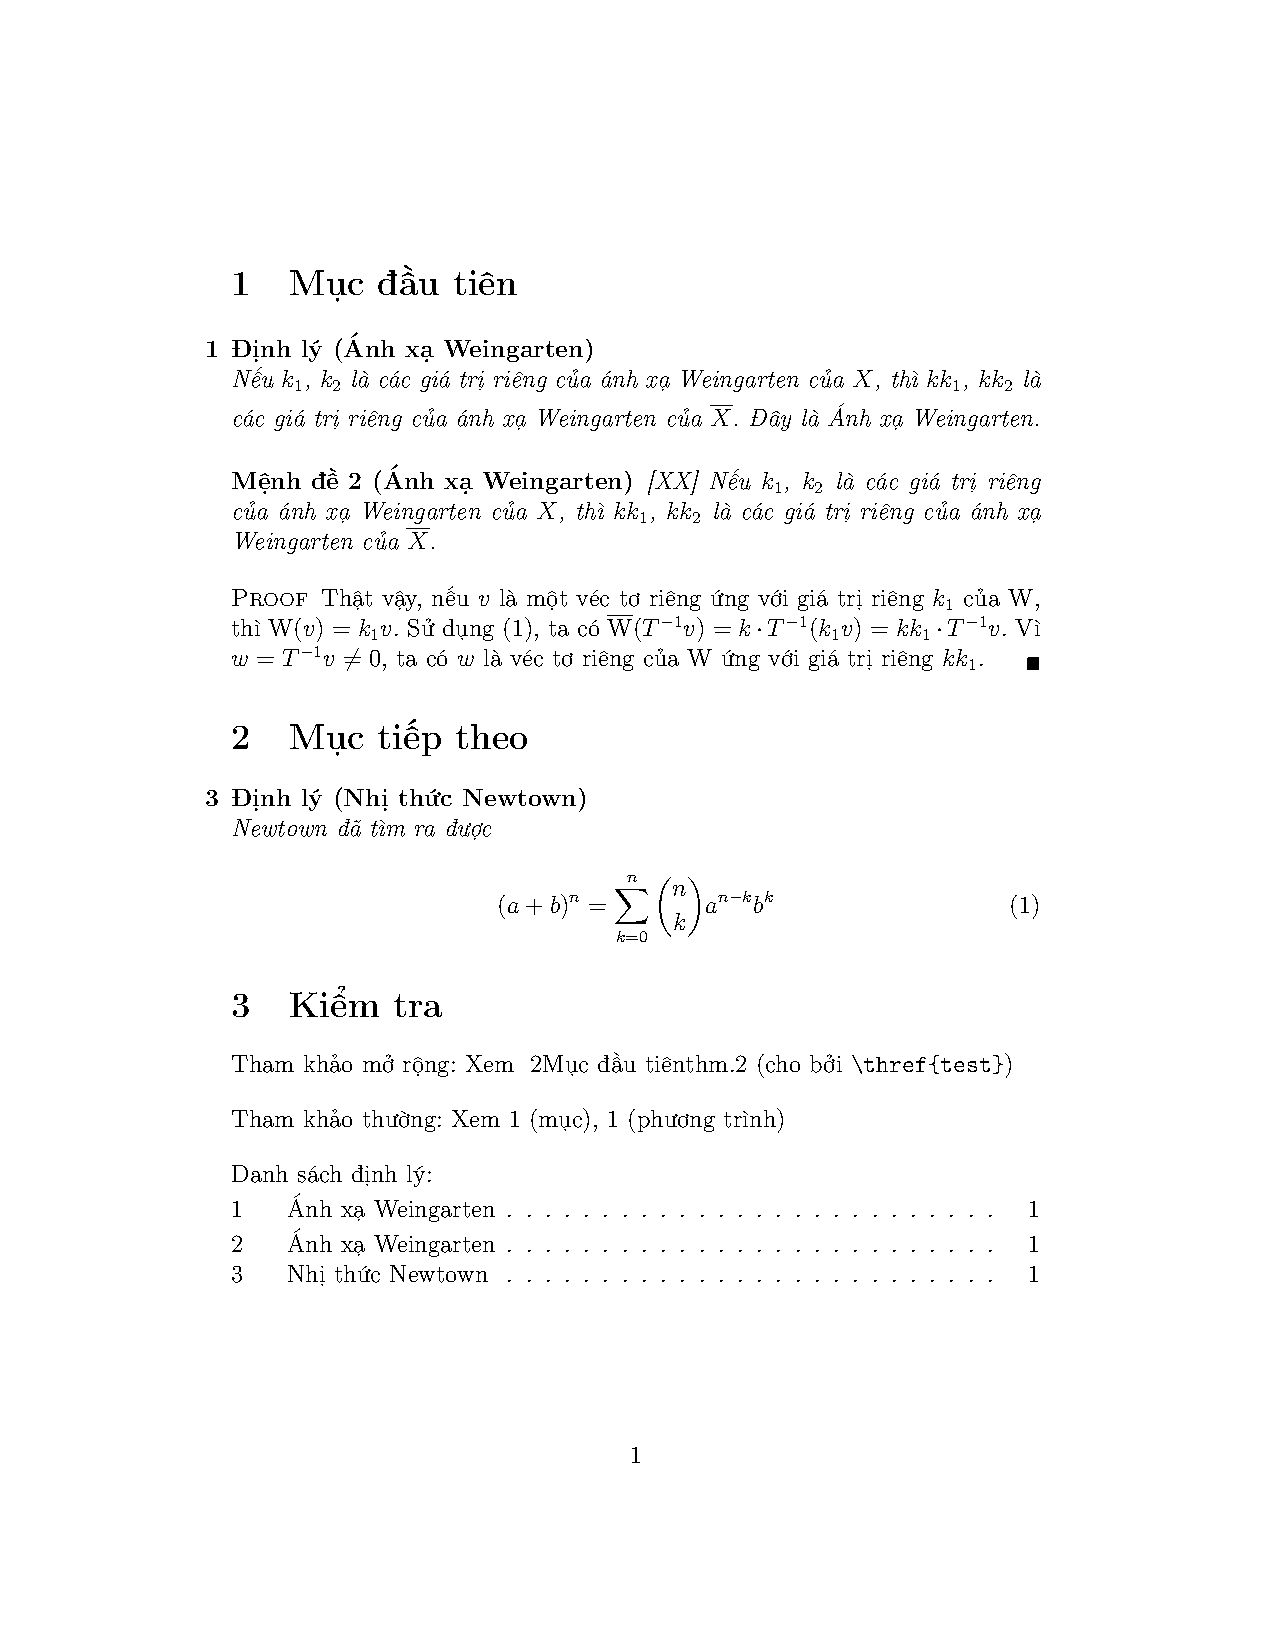
\includegraphics[angle=90,width=0.5\textwidth]{test}
\caption{See on test.}
\end{figure}
\end{verbatim}
\end{code}
Siin lisatakse dokumenti graafika, mis asub failis \texttt{test.eps}.
Graafikat \emph{kõigepealt} pööratakse 90 kraadi võrra ja
\emph{seejärel} skaleeritakse lõpplaiuseni, milleks on 0{,}5 korda
standardse tekstilõigu laius. Kuvasuhe on $1{,}0$, sest kõrgust pole
eraldi määratud. Kõrguse ja laiuse võib anda ka absoluutsetes
mõõtühikutes. Infot ühikute kohta leiab tabelist~\ref{units}
leheküljel~\pageref{units}. Kui on soov selle teema kohta rohkem teada
saada, siis võib lugeda juhendeid \cite{graphics} ja \cite{eps}.

\section{Kirjandusnimestik}

\index{kirjandusnimestik}Kirjandusnimestik luuakse keskkonnas
\ei{thebibliography}. Iga kirje algus on
\begin{lscommand}
\ci{bibitem}\verb|[|\emph{number}\verb|]{|\emph{märgend}\verb|}|
\end{lscommand}
\noindent Dokumendi sees saab siis nime \emph{märgend} kaudu raamatule
või artiklile viidata käsuga
\begin{lscommand}
\ci{cite}\verb|{|\emph{märgend}\verb|}|
\end{lscommand}
Kui suvandit \emph{number} mitte kasutada, siis nummerdatakse kirjed
automaatselt. Käsu \verb|\begin{thebibliography}| järel asuv argument
määrab, kui palju ruumi tähistele jätta. Järgmises näites ütleb
\verb|{99}| \LaTeX ile, et ühegi kirjandusallika järjekorranumber ei ole
laiem kui arv 99.
\begin{example}
Partl~\cite{pa} on
välja pakkunud, et \ldots
\begin{thebibliography}{99}
\bibitem{pa} H.~Partl:
\emph{German \TeX},
TUGboat Volume~9, Issue~1 (1988)
\end{thebibliography}
\end{example}

\chaptermark{Erivahendid} % w need to fix the damage done by the
                          %bibliography example.
\thispagestyle{fancyplain}

Suuremate projektidega töötades tasuks pöörata pilk programmi
\index{BibTeX@Bib\TeX}Bib\TeX{} poole, mis kuulub enamiku \TeX
i-distributsioonide koosseisu. See programm võimaldab hallata
kirjandusviidete andmebaasi ning võtta sealt välja artiklis tsiteeritud
allikate kirjed. Bib\TeX i genereeritud kirjandusnimestike visuaalne
kujundus põhineb stiililehtedel, millega saab kirjandusnimestikke
vormistada laia skaala väljakujunenud stiilide kohaselt.

\section{Aineregister} \label{sec:indexing}

Paljude raamatute väga kasulik osa on \wi{aineregister}. \LaTeX i ja
tugiprogrammiga \wi{MakeIndex}\footnote{Süsteemides, mis ei toeta
failinimesid pikkusega rohkem kui 8 märki, võib selle programmi nimi
olla \texttt{makeidx}.} saab registreid luua üsna
lihtsasti. Käesolev sissejuhatus tutvustab ainult põhilisi registrite
genereerimise käske, sügavamat sissevaadet soovides tuleks pöörduda
raamatu \companion{} poole.

\LaTeX is registri loomiseks tuleb dokumendi preambulis lugeda sisse
pakett \pai{makeidx} käsuga
\begin{lscommand}
\verb|\usepackage{makeidx}|
\end{lscommand}
\noindent ja aktiveerida spetsiaalsed indekseerimiskäsud, lisades
preambulisse käsu
\begin{lscommand}
  \ci{makeindex}
\end{lscommand}
\noindent Registri sisu määratakse käskudega
\begin{lscommand}
  \ci{index}\verb|{|\emph{võti}\verb|@|\emph{registrikirje}\verb|}|
\end{lscommand}
\noindent kus \emph{registrikirje} ilmub registris ja \emph{võti} on
sorteerimisvõti. Argumendi osa \emph{registrikirje} on valikuline. Kui
see puudub, siis võetakse selleks \emph{võti}. Registrikäsud lisatakse
tekstis kohtadesse, kuhu registrikirjed lõppdokumendis peaksid viitama.
Süntaksit on mitme näite kaudu selgitatud tabelis~\ref{index}.

\begin{table}[!hb]
\caption{Registrivõtmete süntaksi näited}\label{index}%
\begin{center}\vskip-\baselineskip
\begin{tabular}{@{}lll@{}}
  \textbf{Näide} &\textbf{Registrikirje} &\textbf{Kommentaar}\\\hline
  \rule{0pt}{1.05em}\verb|\index{tere}| &tere, 1 &Harilik kirje\\
\verb|\index{tere!Peeter}|   &\hspace*{2ex}Peeter, 3 &Alamkirje "`tere"' all\\
\verb|\index{Sass@\textsl{Sass}}|     &\textsl{Sass}, 2& Vormindatud kirje\\
\verb|\index{Liina@\textbf{Liina}}|     &\textbf{Liina}, 7& Vormindatud kirje\\
\verb|\index{Kaese@K\"ase}|     &\textbf{K\"ase}, 33& Vormindatud kirje\\
\verb.\index{ecole@\'ecole}.     &\'ecole, 4& Vormindatud kirje\\
\verb.\index{Jaana|textbf}.     &Jaana, \textbf{3}& Vormindatud leheküljenumber\\
\verb.\index{Joel|textit}.     &Joel, \textit{5}& Vormindatud leheküljenumber
\end{tabular}
\end{center}
\end{table}

Kui \LaTeX{} töötleb sisendfaili, siis kirjutab iga \verb|\index|-käsk
vastava registrikirje koos jooksva leheküljenumbriga teatavasse faili.
Sellel failil on sama nimi nagu \LaTeX i sisendfailil, kuid erinev
laiend (\eei{idx}). Tekkinud faili saab seejärel töödelda programmiga
\wi{MakeIndex}:

\begin{lscommand}
  \texttt{makeindex} \emph{failinimi}
\end{lscommand}
\noindent Programm MakeIndex genereerib sorteeritud registri, millel on
sama failinimi, kuid seekord laiend \eei{ind}. Kui nüüd \LaTeX{}
sisendfaili uuesti töötleb, lisab ta sorteeritud registri dokumendis
kohta, kust ta leiab käsu
\begin{lscommand}
  \ci{printindex}
\end{lscommand}

Pakett \pai{showidx}, mis on \LaTeX iga kaasas, trükib kõik
registrikirjed teksti vasakule äärele. See on üsna kasulik dokumendi
korrektuuriks ja registri kontrollimiseks.

Käsk \ci{index} võib hooletul kasutamisel
mõjutada kujundust:

\begin{example}
Minu Sõna \index{Sõna}. Samas
teine Sõna\index{Sõna}. Pane
tähele punkti asukohta.
\end{example}

Programm MakeIndex ei tunne tähemärke, mis jäävad väljapoole ASCIId.
Korrektseks sorteerimiseks tuleks kasutada märki \verb|@| nagu tabeli
näidetes sõnade K\"ase ja \'ecole puhul.

\section{Kaunid päised}
\label{sec:fancy}

\index{Oostrum, Piet van}Piet van Oostrumi pakett
\pai{fancyhdr}\footnote{\CTAN|pkg/fancyhdr|.} sisaldab paari lihtsat
käsku, millega on võimalik seadistada dokumendi \wi{päis}e- ja
\wi{jalus}erida. Paketi rakendust näeb käesoleva lehekülje ülaääres.

\begin{figure}[!t]
\begin{lined}{\textwidth}
\begin{verbatim}
\documentclass{book}
\usepackage{fancyhdr}
\pagestyle{fancy}
% sellega kindlustame, et peatüki ja jaotise
% pealkirjad kirjutatakse väikeste tähtedega
\renewcommand{\chaptermark}[1]{%
        \markboth{#1}{}}
\renewcommand{\sectionmark}[1]{%
        \markright{\thesection\ #1}}
\fancyhf{}  % kustuta senine päis ja jalus
\fancyhead[LE,RO]{\bfseries\thepage}
\fancyhead[LO]{\bfseries\rightmark}
\fancyhead[RE]{\bfseries\leftmark}
\renewcommand{\headrulewidth}{0.5pt}
\renewcommand{\footrulewidth}{0pt}
\addtolength{\headheight}{0.5pt} % ruum joone jaoks
\fancypagestyle{plain}{%
   \fancyhead{} % eemalda tavalehekülgede päised
   \renewcommand{\headrulewidth}{0pt} % ja joon
}
\end{verbatim}
\end{lined}
\caption{Näiteseadistus paketiga \pai{fancyhdr}} \label{fancyhdr}
\end{figure}

Päiste ja jaluste kohandamisel on keerukas küsimus saada sinna jooksvad
jaotise- ja peatükinimed. \LaTeX{} saavutab selle kaheetapilise
lähenemise teel. Päise ja jaluse definitsioonides esitavad jooksva
jaotise ja jooksva peatüki pealkirju vastavalt käsud \ci{rightmark} ja
\ci{leftmark}. Nende kahe käsu väärtused kirjutatakse üle iga kord, kui
töödeldakse jaotise- või peatükikäsku.

Maksimaalse paindlikkuse huvides ei defineeri käsk \ci{chapter} ja
tema sõbrad käskude \ci{rightmark} ja \ci{leftmark} sisu ise ümber, vaid
nad kutsuvad välja teised käsud (\ci{chaptermark}, \ci{sectionmark} või
\ci{subsectionmark}), mis omakorda defineerivad käskude
\ci{rightmark} ja \ci{leftmark} sisu sobivalt.

Seega, kui vaja on muuta peatüki pealkirja välimust päises, siis tuleb
"`uuendada"' ainult käsku \ci{chaptermark}.
\cih{sectionmark}\cih{subsectionmark}

Joonis~\ref{fancyhdr} kujutab paketi \pai{fancyhdr} võimalikku
seadistust, mille tulemusel näevad päised välja umbes nii nagu käesolevas
raamatukeses. Igal juhul soovitan hankida endale selle paketi
dokumentatsioon allmärkuses nimetatud aadressilt.

\section{Pakett \pai{verbatim}}

Selles raamatus tutvustati eespool \emph{keskkonda} \ei{verbatim}.
Käesolevas jaotises räägime \emph{paketist} \pai{verbatim}. Pakett
\pai{verbatim} on sisuliselt keskkonna \ei{verbatim} ümbertehtud vorm,
mis väldib mõningaid keskkonna \ei{verbatim} puudusi. See iseenesest ei
ole nii mõjuv, kuid paketile \pai{verbatim} on ümbertegemisel lisatud
uut funktsionaalsust, mis ongi põhjus, miks teda siin mainime. Nimelt,
paketis \pai{verbatim} defineeritakse käsk

\begin{lscommand}
\ci{verbatiminput}\verb|{|\emph{failinimi}\verb|}|
\end{lscommand}

\noindent mis võimaldab lisada dokumenti välise ASCII-faili sisu nii,
nagu see asuks keskkonna \ei{verbatim} sees.

Kuivõrd pakett \pai{verbatim} kuulub komplekti Tools, peaks ta olema juba
enamikus süsteemides installitud. Edasist teavet selle paketi kohta saab
juhendist \cite{verbatim}.

\section{Lisapakettide installimine}\label{sec:Packages}

Enamik \LaTeX i installatsioone sisaldab juba suurel hulgal
installitud makropakette, kuid palju rohkem on neid leida võrgust.
Peamine koht, kust Internetis stiilipakette otsida, on CTAN
(\url{http://www.ctan.org}).

Tüüpiliselt koosnevad paketid nagu \pai{geometry}, \pai{hyphenat} ja
paljud teised kahest failist: üks laiendiga \eei{ins} ja teine
laiendiga \eei{dtx}. Sageli on kaasas ka fail \texttt{readme.txt}
paketi lühikirjeldusega. Seda faili tuleks loomulikult lugeda esimesena.

Pärast paketifailide oma masinasse kopeerimist tuleb neid ikkagi veel
töödelda viisil, mis (a) teatab kohalikule \TeX i distributsioonile uue
stiilipaketi olemasolust ja (b) produtseerib dokumentatsiooni. Esimest
osa saab teha nii.

\begin{enumerate}
  \item Käivita \LaTeX{} \wi{INS-fail}il. See pakib lahti \wi{STY-fail}i.
  \item Teisalda STY-fail kohta, kust distributsioon selle üles leiab.
Tavaliselt on selleks alamkataloog \texttt{\ldots/localtexmf/tex/latex}
(Windowsi või OS/2 kasutajad peaksid muutma kaldkriipsude suunda).
  \item Värskenda distributsiooni failinimede andmebaasi. Käsk sõltub
\LaTeX i distributsioonist: süsteemis \index{texlive@\TeX{} Live}\TeX{}
Live sobib \index{texhash@\texttt{texhash}}\texttt{texhash}; süsteemis
\wi{Web2c} \index{mktexlsr@\texttt{mktexlsr}}\texttt{mktexlsr};
süsteemis \index{miktex@MiK\TeX}MiK\TeX{}
\index{initexmf@\texttt{initexmf}}\texttt{initexmf -{}-update-fndb} või
kasutada graafilist kasutajaliidest.
\end{enumerate}

\noindent Nüüd paki lahti DTX-failis olev dokumentatsioon.

\begin{enumerate}
  \item Käivita \LaTeX{} DTX-failil. See genereerib \wi{DVI-fail}i. Vaja
võib olla fail \LaTeX ist läbi lasta mitu korda, enne kui ristviited
paika lähevad.
  \item Kontrolli, kas \LaTeX{} moodustas muude failide seas ka
\wi{IDX-fail}i. Kui seda faili pole, siis dokumentatsioonil puudub register.
Jätka sammust~\ref{step:final}.
  \item Registri genereerimiseks sisesta järgmine rida:
\begin{lscommand}
\texttt{makeindex -s gind.ist }\textit{nimi}
\end{lscommand} (kus \textit{nimi}
on paketi peafaili nimi ilma laiendita).
  \item Käivita \LaTeX{} DTX-failil veel üks kord. \label{step:next}
  \item Viimaks moodusta PS- või PDF-fail, et lugemiselamus oleks
parem.\label{step:final}
\end{enumerate}

Mõnikord võib ilmneda, et moodustunud on veel fail laiendiga \eei{glo}
(sõnastik, glossaar). Anna sammude~\ref{step:next} ja~\ref{step:final}
vahel järgmine käsk:
\begin{lscommand}
\texttt{makeindex -s gglo.ist -o }\textit{nimi}\texttt{.gls
}\textit{nimi}\texttt{.glo}
\end{lscommand}
\noindent Käivita \LaTeX{} DTX-failil veel viimast korda enne üleminekut
sammule~\ref{step:final}.


%%%%%%%%%%%%%%%%%%%%%%%%%%%%%%%%%%%%%%%%%%%%%%%%%%%%%%%%%%%%%%%%%
% Contents: Chapter on pdfLaTeX
% French original by Daniel Flipo 14/07/2004
%%%%%%%%%%%%%%%%%%%%%%%%%%%%%%%%%%%%%%%%%%%%%%%%%%%%%%%%%%%%%%%%%

\section{Töötamine pdf\LaTeX iga} \label{sec:pdftex}
\secby{Daniel Flipo}{Daniel.Flipo@univ-lille1.fr}%
PDF on seadmest sõltumatu hüpertekstidokumentide vorming. Sarnaselt
veebilehega võib dokumendis mõned sõnad märkida
\index{hüperlink}hüperlinkideks, mis viitavad dokumendi muudele
kohtadele või isegi muudele dokumentidele. Hüperlinki klõpsates siirdub
vaade lingi sihtkohta. \LaTeX i kontekstis tähendab see, et kõik käskude
\ci{ref} ja \ci{pageref} esinemised muutuvad hüperlinkideks. Lisaks
muutuvad hüperlinkide kollektsiooniks sisukord, aineregister ja kõik
muud sarnased struktuurid.

Enamik tänapäeva veebilehti on kirjutatud \wi{HTML}-is \emph{(HyperText
Mark"-up Language)}. Teaduslike dokumentide koostamise seisukohalt on
sellel vormingul kaks olulist puudust.
\begin{enumerate}
  \item Valemite lisamist HTML-dokumentidesse üldiselt ei toetata. Kuigi
on olemas vastav standard, enamik brausereid kas ei toeta seda või ei
sisalda vajalikke kirju.
  \item HTML-dokumentide printimine on võimalik, kuid tulemused
varieeruvad suuresti olenevalt platvormist ja brauserist. Tulemused
on kilomeetrite kaugusel kvaliteedist, millega ollakse harjunud \LaTeX i
maailmas.
\end{enumerate}

On tehtud palju katseid luua programme, mis teisendaksid \LaTeX i faile
\wi{HTML}iks. Mõned neist olid üsnagi edukad selles mõttes, et nad
suutsid moodustada loetavaid veebilehti standard-\LaTeX i
sisendfailidest. Kuid kõik nad lõikasid nurki vasakult ja paremalt, et
töö tehtud saaks. Niipea, kui hakata kasutama keerukamaid \LaTeX i
võimalusi ja lisapakette, kipuvad asjad laiali lagunema. Autorid, kes
soovivad säilitada oma dokumentide unikaalset tüpograafilist kvaliteeti
isegi veebis avaldades, pöörduvad seetõttu PDFi (\emph{Portable Document
Format}) poole, mis säilitab kujunduse ja lubab hüpertekstis
navigeerimist. Enamik tänapäevaseid brausereid sisaldab lisasid, mis
suudavad PDF-dokumente otse näidata.

Kuigi pea iga platvormi jaoks on olemas DVI- ja PS-failide
vaatamisprogramme, tuleb välja, et kõige laiemalt on levinud
PDF-failide vaatamiseks mõeldud \wi{Acrobat Reader} ja
\wi{Xpdf}\footnote{\url{http://pdfreaders.org}}. Seetõttu muudab
dokumentide levitamine PDF-versioonidena nad potentsiaalsetele
lugejatele palju kättesaadavamaks.

\subsection{PDF-dokumendid veebi jaoks}

\wi{PDF-fail}i loomine \LaTeX i algtekstist on väga lihtne tänu
programmile \index{pdftex@pdf\TeX}pdf\TeX{}, mille on välja arendanud
H\`an~Th\'{\^e} Th\`anh\index{Th\`anh, H\`an~Th\'{\^e}}. Seal, kus
tavaline \TeX{} moodustab DVI, annab pdf\TeX{} väljundiks PDFi. On
olemas ka programm \index{pdflatex@pdf\LaTeX}pdf\LaTeX, mis genereerib
PDF-väljundi \LaTeX i algtekstist.

Nii pdf\TeX{} kui ka pdf\LaTeX{} installitakse automaatselt enamikus
tänapäevastes \TeX i distributsioonides, nagu
\index{tetex@te\TeX}te\TeX{}, \index{fptex@fp\TeX}fp\TeX{},
\index{miktex@MiK\TeX}MiK\TeX, \index{texlive@\TeX{} Live}\TeX{} Live ja
\index{cmactex@CMac\TeX}CMac\TeX{}.

Selleks, et genereerida DVI asemel PDF, piisab asendada käsk
\texttt{latex fail.tex} käsuga \texttt{pdflatex fail.tex}. Süsteemides,
kus \LaTeX i ei käivitata käsurealt, on selleks tavaliselt omaette nupp
\TeX i graafilises kasutajaliideses.

Paberi suurus määratakse dokumendiklassi valikulise argumendiga, nagu
\texttt{a4paper} või \texttt{letterpaper}. See töötab ka pdf\LaTeX is,
kuid lisaks peab pdf\TeX{} teadma füüsilist paberiformaati, et määrata
lehekülgede füüsiline suurus PDF-failis.\index{paberi formaat} Kasutades
paketti \pai{hyperref} (vt lk \pageref{ssec:pdfhyperref}), seatakse
paberi suurus automaatselt. Muul juhul aga tuleb seda teha käsitsi,
lisades dokumendi preambulisse järgmised read:
\begin{code}
\begin{verbatim}
\pdfpagewidth=\paperwidth
\pdfpageheight=\paperheight
\end{verbatim}
\end{code}

Järgmises jaotises vaadeldakse hariliku \LaTeX i ja pdf\LaTeX i erinevusi
täpsemalt. Peamised erinevused puudutavad kolme valdkonda: kasutatavad
kirjad, lisatavate piltide vorming ja hüperlinkide käsitsi
konfigureerimine.

\subsection{Kirjad}

Programm \index{pdflatex@pdf\LaTeX}pdf\LaTeX{} suudab tegutseda iga sorti
kirjadega (PK raster, TrueType, \PSi{} Type~1, \dots), kuid \LaTeX i
tavapärane kirjavorming, PK raster, paistab dokumenti vaatamisel
\wi{Acrobat Reader}is väga inetu. Hea välimusega dokumentide loomiseks
on kõige parem kasutada ainult \PSi{} Type 1 kirju. Enamik \TeX i
installatsioone seatakse üles nii, et see toimub automaatselt. Kõige
parem on järele proovida. Kui töötab, võib terve selle jaotise vahele
jätta.

Kõige levinum Type 1 kirjakomplekt on tänapäeval
\index{kirjakomplekt!LM}Latin Modern (LM). Uuema \TeX i
installatsiooni puhul on tõenäoline, et need kirjad on juba installitud;
siis on vaja ainult dokumendi preambulisse panna
\begin{code}
\begin{verbatim}
\usepackage{lmodern}
\usepackage[T1]{fontenc}
\usepackage{textcomp}
\end{verbatim}
\end{code}
ja kõik on valmis selleks, et luua täieliku ladina märgikomplekti
täistoetusega suurepärast PDF-väljundit. Töötades aga vähendatud
seadistusega, võib olla tarvis lisada
\index{kirjakomplekt!LM}LM-kirjad eraldi.

\index{vene keel}Vene keele puhul võib kasutada
\index{kirjakomplekt!C1}C1-virtuaalkirju (C1fonts). Need kirjad
ühendavad endas standardsed \index{kirjakomplekt!CM}CM Type 1 kirjad
\index{kirjakomplekt!Blue Sky}Blue Sky kollektsioonist ning
\index{kirjakomplekt!CMCYR}CMCYR Type~1 kirjad
\index{kirjakomplekt!Paradissa}Paradissa ja
\index{kirjakomplekt!BaKoMa}BaKoMa kollektsioonist, mis on kõik
saadaval CTANist. Kuna Paradissa kirjad sisaldavad ainult vene keele
tähti, siis puuduvad C1-kirjades muud \index{kirillitsa}kirillitsa
märgid.

Teine lahendus on minna üle \PSi{} Type~1 kirjadele. Õieti on mõned
neist kaasas \wi{Acrobat Reader}i iga koopiaga. Kuna nendes kirjades on
märkide suurused erinevad, muutub lehekülgede teksti küljendus. Üldiselt
võtavad need muud kirjad rohkem ruumi kui
\index{kirjakomplekt!CM}CM-kirjad, viimased on väga ruumisäästvad.
Samuti kannatab dokumendi kujunduse visuaalne ühtsus, sest
\index{kiri!Times}Times, \index{kiri!Helvetica}Helvetica ja
\index{kiri!Courier}Courier (põhikandidaadid niisuguse asendamise puhul)
ei ole loodud töötama harmoonias ühes ja samas dokumendis.

Selleks eesmärgiks on saadaval kaks valmistehtud kirjakomplekti:
\pai{pxfonts}, milles põhiteksti kiri on \index{kiri!Palatino}Palatino,
ja pakett \pai{txfont}, mille aluseks on \index{kiri!Times}Times. Nende
kasutamiseks piisab lisada dokumendi preambulisse järgmised read:
\begin{code}
\begin{verbatim}
\usepackage[T1]{fontenc}
\usepackage{pxfonts}
\end{verbatim}
\end{code}

Pärast sisendfaili kompileerimist võib leida LOG-failist ridu nagu
\begin{verbatim}
Warning: pdftex (file eurmo10): Font eur... not found
\end{verbatim}
Need tähendavad, et mõnda dokumendis kasutatud kirja ei leitud. Häirivad
kohad dokumendis tuleks kindlasti üles otsida ja ära parandada, sest
vaatamisprogramm ei tarvitse tulemuseks saadud \wi{PDF-fail}i puuduvate
märkidega lehekülgi üldse näidata.

\subsection{Graafika lisamine}
\label{ssec:pdfgraph}\index{joonised}

Graafika lisamine dokumenti töötab kõige paremini paketiga
\pai{graphicx} (vt lk~\pageref{eps}):
\begin{code}
\begin{verbatim}
\usepackage{xcolor,graphicx}
\end{verbatim}
\end{code}
Selles näites loetakse ühtlasi sisse pakett \pai{xcolor} värvi jaoks,
sest veebis kuvatavates dokumentides on värvi kasutamine üsna loomulik.

Nii palju headest uudistest. Halb uudis on see, et \ePSi i
vormingus graafika ei tööta pdf\LaTeX iga. Kui pildifaili lisamiskäsus
\ci{includegraphics} ei ole määratud faili laiendit, siis püüab
\pai{graphicx} sobiva faili ise üles leida, lähtudes suvandi
\emph{draiver} seadetest. Suvandi \texttt{pdftex} puhul sobivad
vormingud \eei{png}, \eei{pdf}, \eei{jpg} ja \eei{mps}
(\MP\index{metapost@\MP}), kuid mitte \eei{eps}.

Selle probleemi lihtne lahendus on konvertida EPS-failid
PDF-vor"-min"-gus"-se
utiliidi \index{epstopdf@\texttt{epstopdf}}\texttt{epstopdf} abil, mis
on olemas paljudes süsteemides. Vektorgraafika (jooniste) puhul on see
hea lahendus. Rastergraafika (fotod, skaneeringud) puhul pole see
ideaalne, sest PDF-vorming toetab loomulikul viisil PNG- ja JPEG-piltide
lisamist. PNG on hea ekraanipiltide ja muude vähese värvide arvuga
piltide jaoks. JPEG sobib hästi fotode jaoks ja on väga ruumisäästev.

Teatavaid geomeetrilisi jooniseid võib isegi olla soovitatav mitte
joonistada, vaid kirjeldada spetsiaalses käsukeeles nagu
\MP\index{metapost@\MP}, mis on olemas enamikus \TeX i
distributsioonides ja tuleb koos omaenda mahuka manuaaliga.

\subsection{Hüpertekstilingid}
\label{ssec:pdfhyperref}

Pakett \pai{hyperref} muudab kõik dokumendi sisemised viited
\index{hüperlink}hüperlinkideks. Et see töötaks, on vaja natuke maagiat,
st dokumendi preambulisse tuleb \emph{viimaseks} käsuks panna
\verb+\usepackage[pdftex]{hyperref}+.

Paketi \pai{hyperref} töö seadistamiseks on palju suvandeid:
\begin{itemize}
\item kas komadega eraldatud loend pärast suvandit \texttt{pdftex}, see
tähendab, \verb+\usepackage[pdftex,+\emph{suvandid}\verb+]{hyperref}+
või
\item üksikud read käskudega
  \ci{hypersetup}\verb+{+\emph{suvandid}\verb+}+.
\end{itemize}

Ainuke nõutav suvand on \texttt{pdftex}, ülejäänud on valikulised ja
võimaldavad muuta paketi \pai{hyperref} tavakäitumist.\footnote{Väärib
märkimist, et pakett \pai{hyperref} ei piirdu ainult pdf\TeX iga, vaid
seda võib konfigureerida paigutama hariliku \LaTeX i poolt loodava
\wi{DVI-fail}i sisse PDFile spetsiifilist informatsiooni, mille
\texttt{dvips} viib edasi \wi{PS-fail}i ja lõpuks PDFi konverter korjab
üles PS-faili teisendamisel
PDFiks.\index{PDF-fail}}\index{dvips@\texttt{dvips}} Järgmises
nimekirjas on vaikeväärtused tähistatud püstkirjaga.

\begin{flushleft}
\begin{description}
  \item [\normalfont\texttt{bookmarks (=true,\textit{false})}] näidata või varjata
    dokumendi kuvamisel järjehoidjariba
  \item [\normalfont\texttt{unicode (=false,\textit{true})}] lubab
\index{Acrobat Reader}Acrobati
järjehoidjates kasutada mitteladina tähestike märke
  \item [\normalfont\texttt{pdftoolbar (=true,\textit{false})}] näidata või varjata
\index{Acrobat Reader}Acrobati tööriistariba
  \item [\normalfont\texttt{pdfmenubar (=true,\textit{false})}] näidata või varjata
\index{Acrobat Reader}Acrobati menüüd
  \item [\normalfont\texttt{pdffitwindow (=false,\textit{true})}] seab
algsuurenduse \wi{PDF-fail}i kuvamisel
  \item [\normalfont\texttt{pdftitle (=\{text\})}] defineerib tiitli, mis
kuvatakse \index{Acrobat Reader}Acrobati dokumendiinfo aknas
  \item [\normalfont\texttt{pdfauthor (=\{text\})}] PDF-faili autori nimi
  \item [\normalfont\texttt{pdfnewwindow (=false,\textit{true})}]
määrab, kas avada uus aken, kui klõpsatav link viib käsilolevast
dokumendist välja
  \item [\normalfont\texttt{colorlinks (=false,\textit{true})}] kas ümbritseda lingid
värviliste raamidega (\texttt{false}) või värvida linkide tekst
(\texttt{true}). Nende linkide värvi võib seadistada järgmiste
suvanditega (näidatud on vaikevärvid):
    \begin{description}
    \item [\normalfont\texttt{linkcolor (=red)}] siselinkide (jaotised,
leheküljed jne) värv
    \item [\normalfont\texttt{citecolor (=green)}] viitelinkide (bibliograafia)
värv
    \item [\normalfont\texttt{filecolor (=magenta)}] faililinkide värv
    \item [\normalfont\texttt{urlcolor (=cyan)}] URL-linkide (e-post, veeb) värv
    \end{description}
\end{description}
\end{flushleft}

Kui vaikeväärtused sobivad, siis võib piirduda käsuga
\begin{code}
\begin{verbatim}
\usepackage[pdftex]{hyperref}
\end{verbatim}
\end{code}

Näiteks et järjehoidjate nimekiri oleks avatud ja lingid oleksid
värvilised (lõppe \texttt{=true} ei ole vaja panna):
\begin{code}
\begin{verbatim}
\usepackage[pdftex,bookmarks,colorlinks]{hyperref}
\end{verbatim}
\end{code}

Printimiseks mõeldud PDFides\index{PDF-fail} pole värvilised lingid
head, sest paberil on nad hallid ning rasked lugeda. Selle asemel võib
kasutada värvilisi raame:
\begin{code}
\begin{verbatim}
\usepackage{hyperref}
\hypersetup{colorlinks=false}
\end{verbatim}
\end{code}
\noindent või muuta lingid mustaks:
\begin{code}
\begin{verbatim}
\usepackage{hyperref}
\hypersetup{colorlinks,%
            citecolor=black,%
            filecolor=black,%
            linkcolor=black,%
            urlcolor=black,%
            pdftex}
\end{verbatim}
\end{code}

Kui tuleb ainult määrata info \wi{PDF-fail}i dokumendiinfo sektsiooni
jaoks:
\begin{code}
\begin{verbatim}
\usepackage[pdfauthor={Pierre Desproges},%
            pdftitle={Des femmes qui tombent},%
            pdftex]{hyperref}
\end{verbatim}
\end{code}

% \vspace{\baselineskip}

Lisaks automaatsetele ristviidete \index{hüperlink}hüperlinkidele on
võimalik dokumenti lisada ka otselinke käsuga
\begin{lscommand}
\ci{href}\verb|{|\emph{url}\verb|}{|\emph{tekst}\verb|}|
\end{lscommand}
\noindent Näiteks kood
\begin{code}
\begin{verbatim}
Organisatsiooni \href{http://www.ctan.org}{CTAN} koduleht.
\end{verbatim}
\end{code}
lisab teksti lingi "`\href{http://www.ctan.org}{CTAN}"';
klõps sõnal "`\textcolor{magenta}{CTAN}"' viib CTANi kodulehele.

Kui lingi sihtkoht ei ole URL, vaid kohalik fail, võib kasutada käsku
\ci{href} ilma osata \texttt{http://}:
\begin{verbatim}
  Täielik dokumentatsioon asub \href{manuaal.pdf}{siin}
\end{verbatim}
mis moodustab teksti "`Täielik dokumentatsioon asub
\textcolor{cyan}{siin}"'. Klõps sõnal "`\textcolor{cyan}{siin}"' avab
faili \texttt{manuaal.pdf}. Failinimi tuleb anda relatiivsena
käsiloleva dokumendi suhtes.

Artikli autor võib soovida anda lugejatele võimaluse talle lihtsasti
kirju saata, mida võib realiseerida nii, et panna dokumendi tiitellehele
käsu \ci{author} sisse käsk \ci{href}:
\begin{code}
\begin{verbatim}
\author{Mary Oetiker $<$\href{mailto:mary@oetiker.ch}%
       {mary@oetiker.ch}$>$}
\end{verbatim}
\end{code}
Tasub tähele panna, et see link on koostatud selliselt, et meiliaadress
oleks olemas ühtaegu nii lingis kui ka leheküljel endal. See on nii
sellepärast, et link \verb+\href{mailto:mary@oetiker.ch}{Mary Oetiker}+
töötaks küll \index{Acrobat Reader}Acrobatis, kuid pärast lehekülje
printimist ei oleks meiliaadress enam nähtav.

\subsection{Probleemid linkidega}

Järgnevat laadi teated
\begin{verbatim}
! pdfTeX warning (ext4): destination with the same identifier
  (name{page.1}) has been already used, duplicate ignored
\end{verbatim}
ilmuvad siis, kui loendur uuesti algväärtustatakse, näiteks
dokumendiklassi \pai{book} käsu \ci{mainmatter} täitmisel. See käsk
seab enne raamatu esimest lehekülge leheküljenumbrite loenduri
väärtuseks 1. Kuid kuna raamatu alguses on samuti olemas lehekülg
number~1, ei ole lingid leheküljele 1 enam üheselt määratud, sellest
teade, et "`duplikaate ignoreeritakse"'.

Vastumeetmena võib \pai{hyperref}i suvanditesse lisada
\texttt{plainpages=false}. See aitab siiski ainult leheküljenumbrite
loenduri puhul. Veelgi radikaalsem lahendus on seada
\texttt{hypertexnames=false}, kuid sellega lakkavad töötamast
lehekülgede lingid aineregistris.

\subsection{Probleemid järjehoidjatega}

Järjehoidjates kuvatav tekst ei näe alati välja nii, nagu soovitud. Et
järjehoidjad on "`ainult tekst"', saab järjehoidjates kuvada vähem
märke kui tavalises \LaTeX i tekstis. Enamasti \pai{hyperref} märkab
selliseid probleeme ja annab hoiatuse:
\begin{code}
\begin{verbatim}
Package hyperref Warning:
Token not allowed in a PDFDocEncoded string:
\end{verbatim}
\end{code}
Selle probleemi lahendus on määratleda järjehoidja jaoks tekstistring,
mis häirivat teksti asendab:
\begin{lscommand}
\ci{texorpdfstring}\verb|{|\emph{\TeX i tekst}\verb|}{|\emph{Järjehoidja tekst}\verb|}|
\end{lscommand}
\noindent Sedalaadi probleemi peamised kandidaadid on matemaatilised
avaldised:
\begin{code}
\begin{verbatim}
\section{\texorpdfstring{$E=mc^2$}%
        {E = mc ** 2}}
\end{verbatim}
\end{code}
muudab valemi \verb+$E=mc^2$+ järjehoidjaalal tekstiks "`E = mc **
2"'.

Kirjutades dokumenti \wi{Unicode}'is ja kasutades järjehoidjates
Unicode'i märkide lubamiseks paketi \pai{hyperref} suvandit
\verb+unicode+, on võimalik käsus \ci{texorpdfstring} valida märke palju
laiemast märgihulgast.

\subsection{Lähtefailide ühilduvus \LaTeX i ja pdf\LaTeX i vahel}
\label{sec:pdfcompat}

Ideaaljuhul võiks dokument kompileeruda ühtviisi hästi nii \LaTeX iga
kui ka \index{pdflatex@pdf\LaTeX}pdf\LaTeX iga. Siin on peamine
probleem graafika\index{joonised} lisamine. Lihtne lahendus on
\emph{süstemaatiliselt loobuda} failinimede laienditest käskudes
\ci{includegraphics}. Need käsud otsivad siis automaatselt jooksvast
kataloogist sobivas vormingus faili. Kõik, mida tuleb teha, on luua
graafikafailidest õiged versioonid. \LaTeX{} otsib faili laiendiga
\eei{eps}, pdf\LaTeX{} aga püüab leida faili, mille laiend on \eei{png},
\eei{pdf}, \eei{jpg} või \eei{mps} (sellises järjekorras).

Olukordade jaoks, kus dokumendi PDF-versiooni jaoks on vaja erinevat
koodi, võib lugeda dokumendi preambulis sisse paketi \pai{ifpdf}%
\footnote{Kogu loo, miks seda paketti kasutada, leiab \TeX i KKK
punktist \url{http://www.tex.ac.uk/FAQ-whatengine.html}.}.
On tõenäoline, et see on juba installitud; kui pole, siis on kasutusel
arvatavasti \index{miktex@MiK\TeX}MiK\TeX,  mis installib puuduva paketi
automaatselt esimesel korral, mil seda püütakse kasutada. See pakett
defineerib spetsiaalse käsu \ci{ifpdf}, mis võimaldab lihtsasti
kirjutada tingimuslikku koodi. Selles näites tahame, et \PSi i versioon
oleks printimiskulude tõttu mustvalge, kuid PDF-versioon veebis
vaatamiseks oleks värviline.
\begin{code}
\begin{verbatim}
\RequirePackage{ifpdf} % Kas luuakse PDFi ?
\documentclass[a4paper,12pt]{book}
\usepackage[latin1]{inputenc}
\usepackage[T1]{fontenc}
\usepackage{lmodern}
\usepackage[bookmarks, % seadista hyperref
            colorlinks,
            plainpages=false]{hyperref}
\usepackage{graphicx}
\ifpdf
  \hypersetup{linkscolor=blue}
\else
  \hypersetup{linkscolors=black}
\fi
\usepackage[english]{babel}
...
\end{verbatim}
\end{code}
Ülaltoodud näites laaditakse pakett \pai{hyperref} isegi siis, kui
PDF-versiooni ei looda. Selle tulemusel töötab käsk \ci{href} kõigil
juhtudel, mistõttu pole vaja käsu iga esinemist ümbritseda
tingimuslausega.

Uuemates \TeX i distributsioonides (nagu \index{texlive@\TeX{}
Live}\TeX{} Live, \index{mactex@Mac\TeX}Mac\TeX{} ja
\index{miktex@MiK\TeX}MiK\TeX{}) on harilik \TeX i programm tegelikult
\index{pdftex@pdf\TeX}pdf\TeX{} ning see lülitub automaatselt PDFi või
DVI loomisele vastavalt nimele, millega ta välja kutsutakse: käsk
\verb|pdflatex| moodustab väljundiks PDFi\index{PDF-fail} ja käsk
\verb|latex| tavalise DVI.\index{DVI-fail}

\section{Töötamine \hologo{XeLaTeX}iga}
\label{sec:xetex}\index{XeTeX@\hologo{XeTeX}}\index{XeLaTeX@\hologo{XeLaTeX}}

\secby{Axel Kielhorn}{A.Kielhorn@web.de}%
Enamik pdf\LaTeX i juures räägitud asju kehtib ka \hologo{XeLaTeX}i
kohta.

Aadressil \url{http://tug.org/xetex} on lehekülg, mis kogub kokku
\hologo{XeTeX}i ja \hologo{XeLaTeX}i puudutavat informatsiooni.

\subsection{Kirjad}

Peale tavaliste, TFM-põhiste kirjade suudab \hologo{XeLaTeX} kasutada
igasugust operatsioonisüsteemile tuntud kirja. Kui süsteemis on
installitud \index{kirjakomplekt!Linux Libertine}Linux Libertine'i
kirjad, siis võib preambulis lihtsalt öelda
\begin{code}
\begin{verbatim}
\usepackage{fontspec}
\setmainfont[Ligatures=TeX]{Linux Libertine}
\end{verbatim}
\end{code}
Enamasti tuvastab see ka kirjade kursiivi- ja paksud versioonid, nii et
käsud \verb|\textit| ja \verb|\textbf| töötavad nagu ikka. Kui kiri
kasutab \index{OpenType}OpenType-teh"-no"-loo"-giat, siis on olemas
juurdepääs paljudele võimalustele, mis varem nõudsid ümberlülitumist
teisele kirjale või virtuaalkirjale. Peamine iseärasus on laiem
märgihulk; kiri võib sisaldada ladina, kreeka ja kirillitsa märke ning
ligatuure.

Paljud kirjad sisaldavad vähemalt kahte liiki numbreid: harilikud
rivistuvad numbrid ja nn vana stiili (ehk väikesed) numbrid, mis
ulatuvad osaliselt alusjoone alla. Kirjad võivad sisaldada
proportsionaalseid numbreid (kus 1 võtab vähem ruumi kui 0) või
ühesuguse laiusega numbreid, mis sobivad tabelite jaoks.

\begin{code}
\begin{verbatim}
\newfontfamily\LLln[Numbers=Lining]{(kiri)}
\newfontfamily\LLos[Numbers=OldStyle]{(kiri)}
\newfontfamily\LLlnm[Numbers=Lining,Numbers=Monospaced]{(kiri)}
\newfontfamily\LLosm[Numbers=OldStyle,Numbers=Monospaced]{(kiri)}
\end{verbatim}
\end{code}

Peaaegu kõik \wi{OpenType}-kirjad sisaldavad
\index{ligatuurid}standardligatuure (fl fi ffi), kuid on ka mõned
haruldased või ajaloolised ligatuurid, nagu st, ct ja tz. Tehnilisse
aruandesse need võib-olla ei sobi, küll aga romaani. Need ligatuurid
saab aktiveerida järgmiste ridadega:

\begin{code}
\begin{verbatim}
\setmainfont[Ligatures=Rare]{(kiri)}
\setmainfont[Ligatures=Historic]{(kiri)}
\setmainfont[Ligatures=Historic,Ligatures=Rare]{(kiri)}
\end{verbatim}
\end{code}

Mitte kõik kirjad ei sisalda mõlemat ligatuuride komplekti, tuleks uurida
kirja dokumentatsiooni või lihtsalt järele proovida. Mõnikord sõltuvad
need ligatuurid keelest, näiteks poola keele ligatuuri fk inglise keeles
ei kasutata. Poola ligatuurid aktiveerib käsk
\begin{code}
\begin{verbatim}
\setmainfont[Language=Polish]{(kiri)}
\end{verbatim}
\end{code}

Mõned kirjad (nagu kommertskiri \index{kiri!Adobe Garmond Premier
Pro}Adobe Garmond Premier Pro) sisaldavad alternatiivseid sümboleid,
mille \index{texlive@\TeX{} Live}\TeX{} Live~2010-ga kaasatulev
\hologo{XeLaTeX} vaikimisi aktiveerib.\footnote{Varasemates versioonides
oli see vaikimisi välja lülitatud.} Tulemuseks on stiilne Q, mille
kriips ulatub järgneva u alla. Selle väljalülitamiseks tuleb defineerida
väljalülitatud kontekstuaalidega kiri:

\begin{code}
\begin{verbatim}
\setmainfont[Contextuals=NoAlternate]{(kiri)}
\end{verbatim}
\end{code}

\hologo{XeLaTeX}i kirjade kohta saab infot paketi \pai{fontspec}
manuaalist.

\subsubsection{Kust saada \wi{OpenType}-kirju?}

Kui installitud on \index{texlive@\TeX{} Live}\TeX{} Live, siis on mõned
neist juba olemas kataloogis \verb|.../texmf-dist/fonts/opentype|, tuleb
lihtsalt nad oma operatsioonisüsteemi installida. Sellesse kollektsiooni
ei kuulu \index{kirjakomplekt!DejaVu}DejaVu kirjad, mis on saadaval
aadressilt \url{http://dejavu-fonts.org}.

Jälgida tuleks, et iga kirja installitakse ainult \emph{üks kord},
muidu võivad ilmneda huvitavad nähtused.

Kasutada võib kõiki arvutisse installitud kirju, kuid tuleb meeles
pidada, et teistel kasutajatel ei tarvitse neid kirju olla. Näiteks
\index{kiri!Zapfino}Zapfino kiri, mida kasutatakse paketi \pai{fontspec}
manuaalis, on olemas Mac OS X-s, aga mitte Windowsi
arvutites.\footnote{Olemas on selle kirja kommertsversioon nimega
\index{kiri!Zapfino Extra}Zapfino Extra.}

\subsubsection{Unicode'i märkide sisestamine}

Märkide arv kirjas on kasvanud, aga klahvide arv tavalisel klaviatuuril
mitte. Kuidas siis mitte-ASCII märke sisestada?

Kirjutades palju teksti võõrkeeles, võib installida selle keele
klaviatuuri ja printida välja klahvide asukohad. (Enamikus
operatsioonisüsteemides on olemas virtuaalne klaviatuur, millest võib
teha ekraanipildi.)

Kui eksootilist sümbolit läheb vaja harva, võib selle lihtsalt valida
märgitabelist.

Mõnes keskkonnas (nt X Windows) on mitte-ASCII märgi sisestamiseks
palju meetodeid. Selliste märkide sisestamiseks pakuvad viise mõned
tekstiredaktorid (nt Vim ja Emacs). Loe oma tööriistade manuaale.

\subsection{Ühilduvus \hologo{XeLaTeX}i ja \hologo{pdfLaTeX}i vahel}

Mõned asjad on \hologo{XeLaTeX}is ja \hologo{pdfLaTeX}is erinevad.

\begin{itemize}
  \item \hologo{XeLaTeX}i dokument peab olema kirjutatud \wi{Unicode}'is
(UTF-8), samas kui \hologo{pdfLaTeX}is võib kasutada paljusid
sisendkodeeringuid.
  \item Pakett \pai{microtype} ei tööta veel \hologo{XeLaTeX}iga, kuid
märkide väljaulatumise tugi on juba arenduses.
  \item Kõik kirjadesse puutuv tuleb üle vaadata (kui ei ole plaanis
jääda \index{kirjakomplekt!LM}Latin Moderni juurde).
\end{itemize}

\section{Esitluste loomine}
\label{sec:beamer}
\secby{Daniel Flipo}{Daniel.Flipo@univ-lille1.fr}
Teadustöö tulemusi võib esitada tahvlil või esitlustarkvara abil
arvutist. \index{pdflatex@pdf\LaTeX}pdf\LaTeX{} koos klassiga
\index{klass!beamer@\textsf{beamer}}\pai{beamer}
võimaldab luua PDF-vormingus esitlusi, mis näevad välja nagu need,
mida saab genereerida \wi{LibreOffice}'iga või \wi{PowerPoint}iga väga heal
päeval, kuid mis on palju portatiivsemad, sest \wi{PDF-fail}ide lugejad on
olemas palju rohkemates süsteemides.

Klass \index{klass!beamer@\textsf{beamer}}\pai{beamer} kasutab pakette \pai{graphicx}, \pai{color} ja
\pai{hyperref} ekraaniesitlustele kohandatud suvanditega.
%La figure~\ref{fig:pdfscr} contient un exemple de fichier minimal ą
%compiler avec \wi{pdf\LaTeX} et le
%résultat produit.

% Écran capturé par ImageMagick (man ImageMagick) fonction « import »
% et convertie en jpg toujours par ImageMagick.

\begin{figure}[htbp]
\begin{verbatim}
\documentclass[10pt]{beamer}
\usepackage[utf8]{inputenc}
\usepackage[T1]{fontenc}
\usepackage[estonian]{babel}
\mode<beamer>{%
  \usetheme[hideothersubsections,
            right,width=22mm]{Goettingen}
}

\title{Lihtne esitlus}
\author[D. Flipo]{Daniel Flipo}
\institute{U.S.T.L. \& GUTenberg}
\titlegraphic{\includegraphics[width=20mm]{USTL}}
\date{2005}

\begin{document}

\begin{frame}<handout:0>
  \titlepage
\end{frame}

\section{Näide}

\begin{frame}
  \frametitle{Mida teha pühapäeva pärastlõunal}
  \begin{block}{Võib \ldots}
    \begin{itemize}
      \item jalutada koera\dots \pause
      \item lugeda raamatut\pause
      \item kimbutada kassi\pause
    \end{itemize}
  \end{block}
  ja palju muud
\end{frame}
\end{document}
\end{verbatim}
  \caption{Klassi \pai{beamer} näitekood}\index{klass!beamer@\textsf{beamer}}
  \label{fig:code-beamer}
\end{figure}

Kompileerides joonisel~\ref{fig:code-beamer} esitatud koodi
\index{pdflatex@pdf\LaTeX}pdf\LaTeX iga, tekib PDF-fail, kus on tiitelleht ja
teine leht loetelupunktidega, mis avatakse ühekaupa esitluse läbimise
käigus.

Üks klassi \index{klass!beamer@\textsf{beamer}}\pai{beamer} eelis on see, et ta loob PDF-faili, mida saab kohe
kasutada, ilma et oleks vaja \PSi i etappi nagu paketi \pai{prosper}
puhul või täiendavat järeltöötlust nagu paketiga \pai{ppower4} loodud
esitluste puhul.

Klassiga \index{klass!beamer@\textsf{beamer}}\pai{beamer} saab luua samast sisendfailist mitu
dokumendiversiooni eri re\v{z}iimide jaoks. Sisendfailis võib
teravsulgudesse <\ldots> kirjutada re\v{z}iime puudutavaid juhiseid.
Olemas on järgmised re\v{z}iimid:
\begin{description}
\item[\normalfont\texttt{beamer}] PDF-esitluse jaoks nagu ülal kirjeldatud;
\item[\normalfont\texttt{trans}] kilede jaoks;
\item[\normalfont\texttt{handout}] prinditud jaotusmaterjali jaoks.
\end{description}
Vaikere\v{z}iim on \texttt{beamer}, selle muutmiseks tuleb uus
re\v{z}iim ette anda globaalse argumendina, näiteks
\verb|\documentclass[10pt,handout]{beamer}| prinditud jaotusmaterjali
jaoks.

Ekraaniesitluse välimus sõltub valitavast teemast. Võib võtta mõne
klassiga \index{klass!beamer@\textsf{beamer}}\pai{beamer} kaasatuleva teema või luua uue. Infot selle kohta
saab klassi dokumentatsioonist \texttt{beameruserguide.pdf}.

Vaatleme täpsemalt koodi joonisel~\ref{fig:code-beamer}. Presentatsiooni
ekraaniversiooni \ci{mode}\verb|<beamer>| jaoks valisime teema
Goettingen, mille puhul kuvatakse slaidil sisukorraga integreeritud
navigatsioonipaneel. Suvandid lubavad valida paneeli suurust (22~mm
praegusel juhul) ja asukohta (põhitekstist paremal). Suvand
\texttt{hideothersubsections} jätab nähtavale kõigi peatükkide
pealkirjad, kuid ainult jooksva peatüki alajaotised. Re\v{z}iimide
\ci{mode}\verb|<trans>| ja \ci{mode}\verb|<handout>| kohta eriseaded
puuduvad, nende kujundus on standardne.

Käskudega \ci{title}, \ci{author}, \ci{institute} ja
\ci{titlegraphic} määratakse tiitellehe sisu. Käskude \ci{title}
ja \ci{author} valikulised argumendid võimaldavad määrata tiitli ja
autori nime erikujud, mis kuvatakse Goettingeni teema
navigatsioonipaneelil.

Paneelil olevad pealkirjad ja alapealkirjad luuakse nagu tavaliselt
käskudega \ci{section} ja \ci{subsection}, mis tuleb panna
\emph{väljapoole} keskkonda \ei{frame}.

Dokumendis saab ringi liikuda ka alaääres olevate väikeste
navigatsiooniikoonide abil. Nende olemasolu ei sõltu valitud teemast.

Iga slaidi või ekraani sisu tuleb panna keskkonna \ei{frame} sisse. On
olemas valikuline argument teravsulgudes (\verb|<| ja \verb|>|), millega
saab raami esitluse mõne versiooni jaoks varjata. Näites on esimene
lehekülg väljajagatavas versioonis nähtamatu argumendi
\verb|<handout:0>| tõttu.

Ülimalt soovitatav on panna igale slaidile, välja arvatud tiitelslaid,
pealkiri. Seda tehakse käsuga \ci{frametitle}. Kui on vaja
alapealkirju, võib kasutada keskkonda \ei{block} nagu näites.
Jaotisekäsud \ci{section} ja \ci{subsection} slaidile endale
väljundit ei jäta.

Loendikeskkonnas lubab käsk \ci{pause} avada punkte ühekaupa. Muid
esitluseefekte pakuvad käsud \ci{only}, \ci{uncover}, \ci{alt}
ja \ci{temporal}. Paljudes kohtades on võimalik kasutada teravsulge
esitluse edasiseks seadistamiseks.

Igal juhul tuleks läbi lugeda failis \texttt{beameruserguide.pdf} asuv
klassi \index{klass!beamer@\textsf{beamer}}\mbox{\pai{beamer}} dokumentatsioon, et saada pilt, mida see
klass võimaldab. Paketti arendatakse aktiivselt ning viimast infot leiab
projekti veebilehelt (\url{https://bitbucket.org/rivanvx/beamer}).

% Local Variables:
% TeX-master: "lshort2e"
% mode: latex
% mode: flyspell
% End:

%%%%%%%%%%%%%%%%%%%%%%%%%%%%%%%%%%%%%%%%%%%%%%%%%%%%%%%%%%%%%%%%%
%%%%%%%%%%%%%%%%%%%%%%%%%%%%%%%%%%%%%%%%%%%%%%%%%%%%%%%%%%%%%%%%%
\setcounter{chapter}{4}
\newcommand{\graphicscompanion}{\emph{The \LaTeX{} Graphics Companion}~\cite{graphicscompanion}} 
\newcommand{\hobby}{\emph{A User's Manual for MetaPost}~\cite{metapost}}
\newcommand{\hoenig}{\emph{\TeX{} Unbound}~\cite{unbound}}
\newcommand{\graphicsinlatex}{\emph{Graphics in \LaTeXe{}}~\cite{ursoswald}}

\chapter{Producción de gráficos matemáticos}
\label{chap:graphics}

\begin{intro}
Mucha gente usa \LaTeX\ para componer sus textos; pero además del enfoque orientado a la estructura (y no al contenido) tan conveniente, \LaTeX\ también ofrece la posibilidad (si bien bastante restringida) de producir salidas gráficas a partir de descripciones textuales.  Por otro lado, se han creado varias extensiones de  \LaTeX\ para evadir estas restricciones.  En esta sección aprenderá algunas de ellas.
\end{intro}

\section{Panorama general}

El entorno \ei{picture} permite programar dibujos directamente en \LaTeX.  Una descripción detallada puede encontrarse en el \manual. Por un lado hay restricciones serias, como que las pendientes de los segmentos de recta así como los radios de los círculos están restringidos a un número corto de valores.  Por otro lado, el entorno \ei{picture} de \LaTeXe\ trae con él la orden \ci{qbezier}, donde ``\texttt{q}'' significa ``cuadrática''.  Muchas curvas usadas con frecuencia, como círculos, elipses o catenarias, puedes aproximarse satisfactoriamente con curvas de  B\'ezier cuadráticas, aunque esto puede requerir algo de matemáticas.  Si además se utiliza un lenguaje de programación como Lisp para generar bloques \ci{qbezier} de \filenomo{}s de entrada \LaTeX, el entorno \ei{picture} se vuelve bastante potente.

Aunque la programación de dibujos directamente en  \LaTeX\ tiene muchas
restricciones, y es a menudo muy incómodo, puede haber razones para hacerlo. Los documentos producidos son ``pequeños'' en cuanto al tamaño en octetos, y no hay que andar  arrastrando \filenomo{}s gráficos adicionales.

Los paqueteos como \pai{epic} y \pai{eepic} (descritos, por ejemplo, en \companion) o \pai{pstricks} ayudan a eliminar las restricciones a las que está sujeto el entorno \ei{picture} original, y refuerzan en gran medida la potencia gráfica de \LaTeX.

Mientras los dos primeros paquetes sólo mejoran el entorno \ei{picture}, el paquete \pai{pstricks} tiene sus propio entorno de dibujo, \ei{pspicture}.  La potencia de  \pai{pstricks} se basa en el hecho de que este paquete hace uso extenso de las posibilidades de \PSi{}.  Además, numerosos paquetes han sido escritos para propósitos específicos.  Uno de ellos es \texorpdfstring{\Xy}{Xy}-pic, descrito al final de este capítulo.  Una amplia variedad de estos paquetes se describe en detalle en \graphicscompanion{} (no lo confunda con \companion).

Quizás la herramienta gráfica más potente relacionada con \LaTeX\ es
\texttt{MetaPost}, el gemelo de \texttt{METAFONT} de Donald E. Knuth. \texttt{MetaPost} tiene el lenguaje de programación de \texttt{METAFONT}, muy potente y matemáticamente sofisticado; pero al contrario que \texttt{METAFONT}, que genera mapas de pixeles, \texttt{MetaPost} genera \filenomo{}s de Encapsulated \PSi{}, que pueden importarse en \LaTeX.  Para una introducción, vea \hobby, o el tutorial de \cite{ursoswald}.

Una discusión minuciosa sobre estrategias en \LaTeX{} y \TeX{} para gráficos (y \fontsnomo{}) puede encontrarse en \hoenig.

\section{El entorno \texttt{picture}}
\secby{Urs Oswald}{osurs@bluewin.ch}

\subsection{Órdenes básicas}

Se crea un entorno \ei{picture}\footnote{Lo crea o no, el entorno picture funciona sin más, con \LaTeXe{} normal, sin necesidad de cargar ningún paquete.} con alguna de las dos órdenes
\begin{lscommand}
\ci{begin}\verb|{picture}(|$x,y$\verb|)|\ldots\ci{end}\verb|{picture}|
\end{lscommand}
o
\begin{lscommand}
\ci{begin}\verb|{picture}(|$x,y$\verb|)(|$x_0,y_0$\verb|)|\ldots\ci{end}\verb|{picture}|
\end{lscommand}
Los números $x,\,y,\,x_0,\,y_0$ se refieren a \ci{unitlength}, que
puede establecerse en cualquier momento
(pero no dentro de un entorno \ei{picture}) con una orden como
\begin{lscommand}
\ci{setlength}\verb|{|\ci{unitlength}\verb|}{1.2cm}|
\end{lscommand}
El valor por omisión de \ci{unitlength} es \texttt{1pt}.  El primer par, $(x,y)$, reserva dentro del documento un espacio rectangular para el dibujo.  El segundo par, opcional, $(x_0,y_0)$, asigna coordenadas arbitrarias a la esquina inferior izquierda del rectángulo reservado.

La mayoría de las órdenes de dibujo tienen alguna de las dos formas
\begin{lscommand}
\ci{put}\verb|(|$x,y$\verb|){|\emph{objeto}\verb|}|
\end{lscommand}
o
\begin{lscommand}
\ci{multiput}\verb|(|$x,y$\verb|)(|$\Delta x,\Delta
y$\verb|){|$n$\verb|}{|\emph{objeto}\verb|}|\end{lscommand}
Las curvas de B\'ezier son una excepción.  Se dibujan con la orden
\begin{lscommand}
\ci{qbezier}\verb|(|$x_1,y_1$\verb|)(|$x_2,y_2$\verb|)(|$x_3,y_3$\verb|)|
\end{lscommand}
\newpage

\subsection{Segmentos de recta}
\begin{example}
\setlength{\unitlength}{5cm}
\begin{picture}(1,1)
  \put(0,0){\line(0,1){1}}
  \put(0,0){\line(1,0){1}}  
  \put(0,0){\line(1,1){1}}  
  \put(0,0){\line(1,2){.5}}
  \put(0,0){\line(1,3){.3333}}
  \put(0,0){\line(1,4){.25}}  
  \put(0,0){\line(1,5){.2}}
  \put(0,0){\line(1,6){.1667}}
  \put(0,0){\line(2,1){1}}
  \put(0,0){\line(2,3){.6667}}
  \put(0,0){\line(2,5){.4}}
  \put(0,0){\line(3,1){1}}  
  \put(0,0){\line(3,2){1}}
  \put(0,0){\line(3,4){.75}}
  \put(0,0){\line(3,5){.6}}
  \put(0,0){\line(4,1){1}}
  \put(0,0){\line(4,3){1}}  
  \put(0,0){\line(4,5){.8}}
  \put(0,0){\line(5,1){1}}
  \put(0,0){\line(5,2){1}}
  \put(0,0){\line(5,3){1}}
  \put(0,0){\line(5,4){1}}
  \put(0,0){\line(5,6){.8333}}
  \put(0,0){\line(6,1){1}}
  \put(0,0){\line(6,5){1}}
\end{picture}
\end{example}
Se dibujan segmentos de recta con la orden
\begin{lscommand}
\ci{put}\verb|(|$x,y$\verb|){|\ci{line}\verb|(|$x_1,y_1$\verb|){|$length$\verb|}}|
\end{lscommand}
La orden \ci{line} tiene dos argumentos:
\begin{enumerate}
  \item un vector director,
  \item una longitud.
\end{enumerate}
Los componentes del vector director están restringidos a los enteros
\[-6,\,-5,\,\ldots,\,5,\,6, \] y tienen que ser primos entre sí (coprimos; sin divisor común salvo 1).  La figura ilustra los 25 posibles valores de las pendientes en el primer cuadrante.  La longitud es relativa a \ci{unitlength}.  El argumento longitud es la coordenada vertical en el caso de un segmento de recta vertical; el el resto de los casos, la coordenada horizontal.

\subsection{Flechas}

\begin{example}
\setlength{\unitlength}{0.75mm}
\begin{picture}(60,40)
  \put(30,20){\vector(1,0){30}}
  \put(30,20){\vector(4,1){20}}
  \put(30,20){\vector(3,1){25}}
  \put(30,20){\vector(2,1){30}}
  \put(30,20){\vector(1,2){10}}
  \thicklines
  \put(30,20){\vector(-4,1){30}}
  \put(30,20){\vector(-1,4){5}}
  \thinlines
  \put(30,20){\vector(-1,-1){5}}
  \put(30,20){\vector(-1,-4){5}}
\end{picture}
\end{example}
Las flechas se dibujan con la orden
\begin{lscommand}
\ci{put}\verb|(|$x,y$\verb|){|\ci{vector}\verb|(|$x_1,y_1$\verb|){|$length$\verb|}}|
\end{lscommand}
Para las flechas, los componentes del vector director están incluso más estrechamente restringidos que para los segmentos de recta, a los enteros \[-4,\,-3,\,\ldots,\,3,\,4. \] Los componentes también tienen que ser primos entre sí (sin divisor común salvo 1).  Fíjese en el efecto de la orden \ci{thicklines} en las dos flechas que apuntan arriba a la izquierda.

\subsection{Circunferencias y círculos}

\begin{example}
\setlength{\unitlength}{1mm}
\begin{picture}(60, 40)
  \put(20,30){\circle{1}}
  \put(20,30){\circle{2}}
  \put(20,30){\circle{4}}
  \put(20,30){\circle{8}}
  \put(20,30){\circle{16}}
  \put(20,30){\circle{32}}
  
  \put(40,30){\circle{1}}
  \put(40,30){\circle{2}}
  \put(40,30){\circle{3}}
  \put(40,30){\circle{4}}
  \put(40,30){\circle{5}}
  \put(40,30){\circle{6}}
  \put(40,30){\circle{7}}
  \put(40,30){\circle{8}}
  \put(40,30){\circle{9}}
  \put(40,30){\circle{10}}
  \put(40,30){\circle{11}}
  \put(40,30){\circle{12}}
  \put(40,30){\circle{13}}
  \put(40,30){\circle{14}}
  
  \put(15,10){\circle*{1}}
  \put(20,10){\circle*{2}}
  \put(25,10){\circle*{3}}
  \put(30,10){\circle*{4}}
  \put(35,10){\circle*{5}}
\end{picture}
\end{example}
La orden
\begin{lscommand}
  \ci{put}\verb|(|$x,y$\verb|){|\ci{circle}\verb|{|\emph{diámetro}\verb|}}|
\end{lscommand}
dibuja una circunferencia con centro $(x,y)$ y diámetro (no radio) \emph{diámetro}. El entorno \ei{picture} sólo admite diámetros hasta aproximadamente 14\,mm, e incluso no todos los diámetros son posibles bajo ese límite.  La orden \ci{circle*} produce discos (círculos rellenos).

Como es el caso de segmentos de recta, uno puede recurrir a paquetes adicionales, como \pai{eepic} o \pai{pstricks}.  Para una descripción minuciosa de estos paquetes, vea \graphicscompanion.

Hay también una posibilidad dentro del entorno \ei{picture}.  Si uno no tiene miedo de hacer los cálculos necesarios (o dejárselo a un programa), circunferencias y elipses arbitrarios pueden parchearse mediante curvas de B\'ezier.  Vea \graphicsinlatex\ para ejemplos y \filenomo{}s en Java.

\subsection{Texto y fórmulas}

\begin{example}
\setlength{\unitlength}{0.8cm}
\begin{picture}(6,5)
  \thicklines
  \put(1,0.5){\line(2,1){3}}
  \put(4,2){\line(-2,1){2}}
  \put(2,3){\line(-2,-5){1}}
  \put(0.7,0.3){$A$}
  \put(4.05,1.9){$B$}
  \put(1.7,2.95){$C$}
  \put(3.1,2.5){$a$}
  \put(1.3,1.7){$b$}
  \put(2.5,1.05){$c$}
  \put(0.3,4){$F=
    \sqrt{s(s-a)(s-b)(s-c)}$}  
  \put(3.5,0.4){$\displaystyle
    s:=\frac{a+b+c}{2}$}
\end{picture}
\end{example}
Como muestra este ejemplo, se pueden escribir texto y fórmulas en un entorno \ei{picture} con la orden \ci{put} de la forma habitual.

\subsection{\ci{multiput} y \ci{linethickness}}

\begin{example}
\setlength{\unitlength}{2mm}
\begin{picture}(30,20)
  \linethickness{0.075mm}
  \multiput(0,0)(1,0){26}%
    {\line(0,1){20}}
  \multiput(0,0)(0,1){21}%
    {\line(1,0){25}}
  \linethickness{0.15mm}    
  \multiput(0,0)(5,0){6}%
    {\line(0,1){20}}
  \multiput(0,0)(0,5){5}%
    {\line(1,0){25}}
  \linethickness{0.3mm}    
  \multiput(5,0)(10,0){2}%
    {\line(0,1){20}}
  \multiput(0,5)(0,10){2}%
    {\line(1,0){25}}
\end{picture}
\end{example}
La orden
\begin{lscommand}
  \ci{multiput}\verb|(|$x,y$\verb|)(|$\Delta x,\Delta
  y$\verb|){|$n$\verb|}{|\emph{objeto}\verb|}|
\end{lscommand}
tiene 4 argumentos: el punto de inicio, el vector de traslación de un objeto al siguiente, el número de objetos y el objeto que dibujar.  La orden \ci{linethickness} se aplica a segmentos de recta horizontales y verticales, pero no a segmentos oblicuos ni a circunferencias.  Sí se aplica, en cambio, a curvas de B\'ezier cuadráticas.

\subsection{Óvalos}

\begin{example}
\setlength{\unitlength}{0.75cm}
\begin{picture}(6,4)
  \linethickness{0.075mm}
  \multiput(0,0)(1,0){7}%
    {\line(0,1){4}}
  \multiput(0,0)(0,1){5}%
    {\line(1,0){6}}
  \thicklines
  \put(2,3){\oval(3,1.8)} 
  \thinlines
  \put(3,2){\oval(3,1.8)} 
  \thicklines
  \put(2,1){\oval(3,1.8)[tl]} 
  \put(4,1){\oval(3,1.8)[b]} 
  \put(4,3){\oval(3,1.8)[r]} 
  \put(3,1.5){\oval(1.8,0.4)}     
\end{picture}
\end{example}
La orden
\begin{lscommand}
  \ci{put}\verb|(|$x,y$\verb|){|\ci{oval}\verb|(|$w,h$\verb|)}|
\end{lscommand}
o
\begin{lscommand}
  \ci{put}\verb|(|$x,y$\verb|){|\ci{oval}\verb|(|$w,h$\verb|)[|\emph{posición}\verb|]}|
\end{lscommand}
produce un óvalo centrado en $(x,y)$ y con una anchura $w$ y altura $h$.  Los argumentos opcionales de \emph{posición}  \texttt{t}, \texttt{b}, \texttt{l}, \texttt{r} se refieren a ``top'' (arriba), ``bottom'' (abajo), ``left'' (izquierda), ``right''(derecha), y pueden combinarse, como ilustra el ejemplo.

El grosor de la línea puede controlarse con dos tipos de órdenes: \\ 
\ci{linethickness}\verb|{|\emph{longitud}\verb|}| por un lado, \ci{thinlines} y \ci{thicklines} por el otro.  Mientras \ci{linethickness}\verb|{|\emph{longitud}\verb|}| se aplica sólo a líneas horizontales y verticales (y curvas de B\'ezier cuadráticas), \ci{thinlines} y \ci{thicklines} se aplican a segmentos de recta oblicuos y a circunferencias y óvalos.

\subsection{Uso múltiple de cajas de dibujos predefinidas}

\begin{example}
\setlength{\unitlength}{0.5mm}
\begin{picture}(120,168)
\newsavebox{\foldera}
\savebox{\foldera}
  (40,32)[bl]{% definición
  \multiput(0,0)(0,28){2}
    {\line(1,0){40}}
  \multiput(0,0)(40,0){2}
    {\line(0,1){28}}
  \put(1,28){\oval(2,2)[tl]}
  \put(1,29){\line(1,0){5}}
  \put(9,29){\oval(6,6)[tl]}
  \put(9,32){\line(1,0){8}}
  \put(17,29){\oval(6,6)[tr]}
  \put(20,29){\line(1,0){19}}
  \put(39,28){\oval(2,2)[tr]}  
}
\newsavebox{\folderb}
\savebox{\folderb}
  (40,32)[l]{%         definición
  \put(0,14){\line(1,0){8}}
  \put(8,0){\usebox{\foldera}}
}
\put(34,26){\line(0,1){102}} 
\put(14,128){\usebox{\foldera}}
\multiput(34,86)(0,-37){3}
  {\usebox{\folderb}} 
\end{picture}
\end{example}
Una caja de dibujo puede  \emph{declararse} con la orden
\begin{lscommand}
  \ci{newsavebox}\verb|{|\emph{nombre}\verb|}|
\end{lscommand}
y después \emph{definirse} con  
\begin{lscommand}
  \ci{savebox}\verb|{|\emph{nombre}\verb|}(|\emph{anchura,altura}\verb|)[|\emph{posición}\verb|]{|\emph{contenido}\verb|}|
\end{lscommand}
y finalmente puede \emph{dibujarse} cuantas veces se desee con
\begin{lscommand}
  \ci{put}\verb|(|$x,y$\verb|)|\ci{usebox}\verb|{|\emph{nombre}\verb|}|
\end{lscommand}

El parámetro opcional  \emph{posición} tiene el efecto de definir el `punto de anclaje' de la caja.  En el ejemplo se establece a \texttt{bl}, lo que pone el punto de anclaje en la esquina inferior izquierda (bottom left) de la caja.  Los otros indicadores de posición son \texttt{t}op (superior) y \texttt{r}ight (derecha).

El argumento \emph{nombre} se refiere a un espacio de almacenamiento de  \LaTeX{}  y, por tanto, su aspecto ha de ser como el de una orden (lo que implica las retrobarras en el ejemplo).  Las cajas de dibujo pueden anidarse: En este ejemplo, \ci{foldera} se usa dentro de la definción de \ci{folderb}.

Tiene que usarse la orden \ci{oval} pues la orden \ci{line} no funciona si la longitud del segmento en menor de  3\,mm.

\subsection{Curvas de B\'ezier cuadráticas}

\begin{example}
\setlength{\unitlength}{0.8cm}
\begin{picture}(6,4)
  \linethickness{0.075mm}
  \multiput(0,0)(1,0){7}
    {\line(0,1){4}}
  \multiput(0,0)(0,1){5}
    {\line(1,0){6}}
  \thicklines
  \put(0.5,0.5){\line(1,5){0.5}}    
  \put(1,3){\line(4,1){2}} 
  \qbezier(0.5,0.5)(1,3)(3,3.5)
  \thinlines   
  \put(2.5,2){\line(2,-1){3}}
  \put(5.5,0.5){\line(-1,5){0.5}}
  \linethickness{1mm}
  \qbezier(2.5,2)(5.5,0.5)(5,3)
  \thinlines
  \qbezier(4,2)(4,3)(3,3)
  \qbezier(3,3)(2,3)(2,2)
  \qbezier(2,2)(2,1)(3,1)
  \qbezier(3,1)(4,1)(4,2)
\end{picture}
\end{example}
Como ilustra este ejemplo, dividir un círculo en 4 curvas de B\'ezier cuadráticas no es satisfactorio.  Al menos se necesitan 8.  La figura muestra de nuevo el efecto de la orden \ci{linethickness} en las rectas verticales u horizontales, y de las órdenes \ci{thinlines} y \ci{thicklines} en los segmentos oblicuos.  También muestra que ambos tipos de órdenes afectan a las curvas de  B\'ezier cuadráticas, de forma que cada orden se impone sobre las anteriores.

Indiquen $P_1=(x_1,\,y_1),\,P_2=(x_2,\,y_2)$ los puntos extremos, y $m_1,\,m_2$ las pendientes respectivas, de una curva de B\'ezier cuadrática.  El punto de control intermedio $S=(x,\,y)$ viene dado por la ecuación
\begin{equation} \label{zwischenpunkt}
  \left\{
    \begin{array}{rcl}
      x & = & \displaystyle \frac{m_2 x_2-m_1x_1-(y_2-y_1)}{m_2-m_1}, \\
      y & = & y_i+m_i(x-x_i)\qquad (i=1,\,2).
    \end{array}
  \right.
\end{equation}
Vea \graphicsinlatex\ para un programa en Java que genera la línea de órdenes \ci{qbezier} necesaria.

\subsection{Catenaria}

\begin{example}
\setlength{\unitlength}{1cm}
\begin{picture}(4.3,3.6)(-2.5,-0.25)
\put(-2,0){\vector(1,0){4.4}}
\put(2.45,-.05){$x$}
\put(0,0){\vector(0,1){3.2}}
\put(0,3.35){\makebox(0,0){$y$}}
\qbezier(0.0,0.0)(1.2384,0.0)
  (2.0,2.7622) 
\qbezier(0.0,0.0)(-1.2384,0.0)
  (-2.0,2.7622)
\linethickness{.075mm}
\multiput(-2,0)(1,0){5}
  {\line(0,1){3}}
\multiput(-2,0)(0,1){4}
  {\line(1,0){4}}
\linethickness{.2mm}
\put( .3,.12763){\line(1,0){.4}}
\put(.5,-.07237){\line(0,1){.4}}
\put(-.7,.12763){\line(1,0){.4}}
\put(-.5,-.07237){\line(0,1){.4}}
\put(.8,.54308){\line(1,0){.4}}
\put(1,.34308){\line(0,1){.4}}
\put(-1.2,.54308){\line(1,0){.4}}
\put(-1,.34308){\line(0,1){.4}}
\put(1.3,1.35241){\line(1,0){.4}}
\put(1.5,1.15241){\line(0,1){.4}}
\put(-1.7,1.35241){\line(1,0){.4}}
\put(-1.5,1.15241){\line(0,1){.4}}
\put(-2.5,-0.25){\circle*{0.2}}
\end{picture}
\end{example}

En esta figura, cada mitad simétrica de la catenaria $y=\cosh x -1$ se aproxima mediante una curva de B\'ezier cuadrática.  La mitad derecha de la curva acaba en el punto \((2;\,2.7622)\), y la pendiente allí tiene el valor \(m=3.6269\).  Usando de nuevo la ecuación  (\ref{zwischenpunkt}), podemos calcular los puntos de control intermedios.  Resultan ser $(1.2384;\,0)$ y $(-1.2384;\,0)$.  Las cruces indican puntos de la catenaria \emph{real}.  El error es difícilmente percibible, al ser menor del uno por ciento.

Este ejemplo incluye el uso del argumento opcional de la orden \\
\verb|\begin{picture}|. El dibujo se define en coordenadas ``matemáticas'' convenientes, mientras con la orden
\begin{lscommand} 
  \ci{begin}\verb|{picture}(4.3,3.6)(-2.5,-0.25)|
\end{lscommand}
a su esquina inferior izquierda (marcada con un círculo negro) se le asignan coordenadas $(-2.5;-0.25)$. 

\subsection{Rapidez en la Teoría Especial de la Relatividad}

\begin{example}
\setlength{\unitlength}{0.8cm}
\begin{picture}(6,4)(-3,-2)
  \put(-2.5,0){\vector(1,0){5}}
  \put(2.7,-0.1){$\chi$}
  \put(0,-1.5){\vector(0,1){3}}
  \multiput(-2.5,1)(0.4,0){13}
    {\line(1,0){0.2}}
  \multiput(-2.5,-1)(0.4,0){13}
    {\line(1,0){0.2}}
  \put(0.2,1.4)
    {$\beta=v/c=\tanh\chi$}
  \qbezier(0,0)(0.8853,0.8853)
    (2,0.9640)
  \qbezier(0,0)(-0.8853,-0.8853)
    (-2,-0.9640)
  \put(-3,-2){\circle*{0.2}}
\end{picture}
\end{example}
Los puntos de control de las dos curvas de B\'ezier se calcularon con las fórmulas (\ref{zwischenpunkt}).  La rama positiva se determina con $P_1=(0;\,0),\,m_1=1$ y $P_2=(2;\,\tanh 2),\,m_2=1/\cosh^2 2$.  De nuevo, el dibujo se define en coordenadas matemáticas convenientes, y a la esquina inferior izquierda se le asignan las coordenadas matemáticas $(-3;-2)$ (círculo negro).

\section{Los paquetes graficos PGF y TikZ} % (fold)
\label{sec:tikz}

Hoy en día todos los sistemas de generación de salida de \LaTeX{} pueden crear agradables gráficos vectoriales, es sólo que las interfaces son bastante diversas. El paquete \pai{pgf} proporciona una capa de abstracción sobre estas interfaces. El paquete \pai{pgf} viene con un gran manual/tutorial propio~\cite{pgfplot}. Así que sólo vamos a arañar la superficie del paquete con esta pequeña sección.

El paquete \pai{pgf} viene con un lenguaje de alto nivel de acceso proporcionado por el paquete \pai{tikz}. TikZ proporciona comandos altamente eficientes para dibujar gráficos correctamente dentro de su documento. Utilice el entorno \ei{tikzpicture} para agrupar sus comandos TikZ.

Como se mencionó anteriormente, hay un excelente manual para \pai{pgf} y compañía. Así que en lugar de explicar realmente cómo funciona, les mostraré algunos ejemplos para que puedan obtener una primera impresión de cómo funciona esta herramienta.

En primer lugar un diagrama simple sin sentido.
\begin{example}
\begin{tikzpicture}[scale=3]
  \clip (-0.1,-0.2)
     rectangle (1.8,1.2);
  \draw[step=.25cm,gray,very thin]
       (-1.4,-1.4) grid (3.4,3.4);
  \draw (-1.5,0) -- (2.5,0);
  \draw (0,-1.5) -- (0,1.5);
  \draw (0,0) circle (1cm);
  \filldraw[fill=green!20!white,
            draw=green!50!black]
    (0,0) -- (3mm,0mm) 
         arc (0:30:3mm) -- cycle;
\end{tikzpicture}
\end{example}
Observe el carácter punto y coma (\texttt{;}). Separa los comandos individuales.

Un simple diagrama  de Venn
\begin{example}
\shorthandoff{:}
\begin{tikzpicture}
  \node[circle,draw,
        minimum size=3cm,
        label=120:{economía}]
         at (0,0) {};
  \node[circle,draw,
        minimum size=3cm,
        label=60:{psicología}]
         at (1,0) {};
  \node (i) at (0.5,-1) {};
  \node at (0.6,-2.5) 
    {economía conductual}
    edge[->,thick,
         out=60,in=-60] (i);
\end{tikzpicture}
\end{example}
Si está utilizando \pai{TikZ} en relación con \pai{babel} algunos de los caracteres utilizados en el lenguaje TikZ pueden ser modificados por \pai{babel}, lo que lleva a errores singulares. Para contrarrestar este problema, agregue el comando \ci{shorthandoff} a su código.

Observe los bucles foreach en el siguiente ejemplo.
\begin{example}
\begin{tikzpicture}[scale=0.8]
  \tikzstyle{v}=[circle, minimum size=2mm,inner sep=0pt,draw]
  \foreach \i in {1,...,8}
    \foreach \j in {1,...,3}
      \node[v] 
        (G-\i-\j) at (\i,\j) {};
  \foreach \i in {1,...,8}
    \foreach \j/\o in {1/2,2/3}
      \draw[->] 
        (G-\i-\j) -- (G-\i-\o);
  \foreach \i/\n in 
    {1/2,2/3,3/4,4/5,5/6,6/7,7/8}
    \foreach \j/\o in {1/2,2/3} {
       \draw[->] (G-\i-\j) -- (G-\n-\o);
       \draw[->] (G-\n-\j) -- (G-\i-\o);
    }
\end{tikzpicture}
\end{example}

Con la orden \ci{usetikzlibrary} en el preámbulo puede habilitar una amplia variedad de características adicionales para dibujar formas especiales, como esta caja que está ligeramente curvada.
\begin{example}
\usetikzlibrary{%
  decorations.pathmorphing}
\begin{tikzpicture}[
     decoration={bent,aspect=.3}]
 \draw [decorate,fill=lightgray]
        (0,0) rectangle (5.5,4);
 \node[circle,draw] 
        (A) at (.5,.5) {A};
 \node[circle,draw] 
        (B) at (5,3.5) {B};
 \draw[->,decorate] (A) -- (B);
 \draw[->,decorate] (B) -- (A);
\end{tikzpicture}
\end{example}

\begin{example}
\usetikzlibrary{positioning}
\begin{tikzpicture}[xscale=6,
     yscale=8,>=stealth]
  \tikzstyle{v}=[circle,
     minimum size=1mm,draw,thick]
  \node[v] (a) {$1$};
  \node[v] (b) [right=of a] {$2$};
  \node[v] (c) [below=of a] {$2$};
  \node[v] (d) [below=of b] {$1$};
  \draw[thick,->] 
        (a) to node {} (c);
  \draw[thick,->] 
        (a) to node {} (d);
  \draw[thick,->] 
        (b) to node {} (d);
\end{tikzpicture}
\end{example}
 
 Incluso puede dibujar diagramas de sintaxis que se ven como si vinieran directamente de un libro sobre programación en Pascal. El código es un poco más intimidante que el ejemplo anterior, por lo que sólo mostraré el resultado. Si usted echa un vistazo en la documentación de \pai{pgf} encontrará un tutorial detallado sobre la elaboración de este diagrama exacto.

 \begin{center}
\begin{tikzpicture}[point/.style={coordinate},thick,draw=black!50,>=stealth',
                    tip/.style={->,shorten >=1pt},every join/.style={rounded corners},
                    skip loop/.style={to path={-- ++(0,#1) -| (\tikztotarget)}},
                    hv path/.style={to path={-| (\tikztotarget)}},
                    vh path/.style={to path={|- (\tikztotarget)}},
                 terminal/.style={
            rounded rectangle,
            minimum size=6mm,
            thick,draw=black!50,
            top color=white,bottom color=black!20,
            font=\ttfamily\tiny},
                nonterminal/.style={
                       rectangle,
                       minimum size=6mm,
                       thick,
                       draw=red!50!black!50,         % 50% red and 50% black,
                       top color=white,              % a shading that is white at the top...
                       bottom color=red!50!black!20, % and something else at the bottom
                       font=\itshape\tiny}]
\matrix[column sep=4mm] {
  % First row:
  & & & & & & & & & & & \node (plus) [terminal] {+};\\
  % Second row:
  \node (p1) [point] {}; &     \node (ui1)    [nonterminal] {entero sin signo}; &
  \node (p2) [point] {}; &     \node (dot)    [terminal]    {.};                &
  \node (p3) [point] {}; &     \node (digit) [terminal]     {dígito};            &
  \node (p4) [point] {}; &     \node (p5)     [point] {};                       &
  \node (p6) [point] {}; &     \node (e)      [terminal]    {E};                &
  \node (p7) [point] {}; &                                                      &
  \node (p8) [point] {}; &     \node (ui2)    [nonterminal] {entero sin signo}; &
  \node (p9) [point] {}; &     \node (p10)    [point]       {};\\
  % Third row:
  & & & & & & & & & & & \node (minus)[terminal] {-};\\
};
{ [start chain]
  \chainin (p1);
  \chainin (ui1)   [join=by tip];
  \chainin (p2)    [join];
  \chainin (dot)   [join=by tip];
  \chainin (p3)    [join];
  \chainin (digit) [join=by tip];
  \chainin (p4)    [join];
  { [start branch=digit loop]
    \chainin (p3) [join=by {skip loop=-6mm,tip}];
  }
  \chainin (p5)    [join,join=with p2 by {skip loop=6mm,tip}];
  \chainin (p6)    [join];
  \chainin (e)     [join=by tip];
  \chainin (p7)    [join];
  { [start branch=plus]
    \chainin (plus) [join=by {vh path,tip}];
    \chainin (p8)    [join=by {hv path,tip}];
  }
  { [start branch=minus]
    \chainin (minus) [join=by {vh path,tip}];
    \chainin (p8)    [join=by {hv path,tip}];
  }
  \chainin (p8)    [join];
  \chainin (ui2)   [join=by tip];
  \chainin (p9)    [join,join=with p6 by {skip loop=-11mm,tip}];
  \chainin (p10)   [join=by tip];
}
\end{tikzpicture}
\end{center}

Y hay más, si tiene que dibujar gráficas de datos o funciones numéricas, usted puede echar un vistazo más de cerca al paquete \pai{pgfplot}. Ofrece todo lo necesario para dibujar gráficos. Incluso puede llamar al comando externo \texttt{gnuplot} para evaluar las funciones reales que trazó en el gráfico.

Para una mayor inspiración, asegúrese de visitar la excelente página \linebreak \url{http://www.texample.net/tikz/} de Kjell Magne Fauske que contiene un depósito cada vez más grande de hermosos gráficos y otro tipo de código \LaTeX{}. En \TeX{}ample.net también encontrará una  \href{http://www.texample.net/tikz/resources/#tools-that-generate-pgftikz-code}{lista de herramientas} para trabajar con PGF/TikZ de modo que usted no tenga que escribir todo ese código a mano.

%%% Local Variables:
%%% TeX-master: "lshort.tex"
%%% mode: flyspell
%%% TeX-PDF-mode: t
%%% End:
%%%%%%%%%%%%%%%%%%%%%%%%%%%%%%%%%%%%%%%%%%%%%%%%%%%%%%%%%%%%%%%%%
% Contents: Customising LaTeX output
%%%%%%%%%%%%%%%%%%%%%%%%%%%%%%%%%%%%%%%%%%%%%%%%%%%%%%%%%%%%%%%%%
\chapter{Personalización de \LaTeX}

\begin{intro}
Los documentos producidos mediante las órdenes que ha aprendido hasta este punto parecerán aceptables a una amplia audiencia.  Aunque no tienen un aspecto extraordinario, obedecen todas las reglas establecidas de composición correcta, lo que los hará fáciles de leer y plácidos a la vista.

Sin embargo, hay situaciones donde \LaTeX{} no proporciona una orden o entorno que cubra sus necesidades, o la salida producida por algunas órdenes existentes puede no satisfacer sus expectativas.

En este capítulo, se darán algunas pistas para enseñar a \LaTeX{} nuevos trucos y hacerle producir salidas con diferente aspecto del producido por omisión.
\end{intro}


\section{Nuevas órdenes, entornos y paquetes}

Puede haber notado que todas las órdenes que presento en este libro se componen en una caja, y que se muestran en el índice al final del libro.  En lugar de usar directamente las órdenes \LaTeX{} necesarias para conseguirlo, he creado un \wi{paquete} en que defino nuevas órdenes y entornos con este propósito.  Ahora puedo escribir simplemente:

\begin{example}
\begin{lscommand}
\ci{dum}
\end{lscommand}
\end{example}

En este ejemplo, estoy usando tanto un nuevo entorno llamado\\ \ei{lscommand}, que es responsable de dibujar la caja alrededor de la orden, y una nueva orden llamada \ci{ci}, que compone el nombre de la orden y hace la correspondiente entrada en el índice.  Puede comprobarlo buscando la orden \ci{dum} en el índice al final del libro, donde pude encontrar una entrada para \ci{dum}, apuntando a cada página donde he mencionado la orden \ci{dum}.

Si alguna vez decido que no me gusta que las órdenes se compongan en una caja, puedo simplemente cambiar la definición del entorno \texttt{lscommand} para crear un nuevo aspecto.  Esto es mucho más fácil que ir por todo el documento localizando todos los lugares en que he usado comandos \LaTeX{} genéricos para dibujar una caja alrededor de una palabra.


\subsection{Órdenes nuevas}

Para añadir sus órdenes nuevas, use la orden
\begin{lscommand}
\ci{newcommand}\verb|{|%
       \emph{nombre}\verb|}[|\emph{núm}\verb|]{|\emph{definición}\verb|}|
\end{lscommand}
%command. 
Básicamente, lo orden requiere dos argumentos: el \emph{nombre} de la orden que quiere crear, y la \emph{definición} de la orden.  El argumento \emph{núm} entre corchetes es opcional e indica el número de argumentos que toma la nueva orden (hasta 9 son posibles).  Si no se indica el valor es 0, es decir, no se permiten argumentos.

Los siguientes dos ejemplos deberían ayudarle a entender la idea. El primer ejemplo define una nueva orden llamada \ci{intc}.  Es la abreviatura de ``La introducción no-tan-corta a \LaTeXe''.  Tal orden podría ser útil si tuviera que escribir el título del libro una y otra vez.

\begin{example}
\newcommand{\intc}{La 
    introducción no-tan-corta a
    \LaTeXe}
Esto es ``\intc'' \ldots{} 
``\intc''
\end{example}

El siguiente ejemplo ilustra cómo definir una orden nueva que toma un argumento. Los caracteres \verb|#1| se sustituyen por el argumento indicado.  Si quisiera usar un segundo argumento, use \verb|#2| y así sucesivamente.

\begin{example}
\newcommand{\txsit}[1]
 {Esta es la Introducción
   \emph{#1}-corta a \LaTeXe}
% en el cuerpo del documento: 
\begin{itemize}
    \item \txsit{no-tan}
    \item \txsit{súper}
\end{itemize}
\end{example}

\LaTeX{} no le permitirá crear una nueva orden sobre una ya existente.  Pero hay una orden especial en el caso de que explícitamente quisiera reemplazarla: \ci{renewcommand}. Usa la misma sintaxis que la orden \verb|\newcommand|.

En ciertos casos puede querer usar la orden \ci{providecommand}.  Funciona como \ci{newcommand} y hace que la orden sea definida si aún no existe, pero no hace nada si ya estaba definida.

Hay algunos puntos que comentar sobre los espacios que siguen a las órdenes de \LaTeX{}.  Vea la página  \pageref{whitespace} para más información.

\subsection{Nuevos entornos}

Similar a la orden \verb|\newcommand|, hay una orden para crear sus propios entornos.  La orden \ci{newenvironment} usa la siguiente sintaxis:

\begin{lscommand}
\ci{newenvironment}\verb|{|%
       \emph{nombre}\verb|}[|\emph{núm}\verb|]{|%
       \emph{antes}\verb|}{|\emph{después}\verb|}|
\end{lscommand}

También \ci{newenvironment} puede tener un argumento opcional.  El material indicado en el argumento \emph{antes} se procesa antes de que se procese el texto del entorno.  El material en el argumento \emph{después} se procesa cuando se encuentra la orden \verb|\end{|\emph{nombre}\verb|}|.

El ejemplo siguiente ilustra el uso de la orden \ci{newenvironment}.
\begin{example}
\newenvironment{king}
 {\rule{1ex}{1ex}%
      \hspace{\stretch{1}}}
 {\hspace{\stretch{1}}%
      \rule{1ex}{1ex}}

\begin{king} 
Mis humildes ideas\ldots
\end{king}
\end{example}

El argumento \emph{núm} se usa igual que con la orden \verb|\newcommand|. \LaTeX{} se asegura de que usted no defina un entorno que ya existe; pero si quiere alguna vez cambiar un entorno existente, puede usar la orden \ci{renewenvironment}.  Usa la misma sintaxis que la orden \ci{newenvironment}.

La orden usada en este ejemplo se explicará más tarde.  Para la orden \ci{rule} véase la página \pageref{sec:rule}, para \ci{stretch} vaya a la página \pageref{cmd:stretch}, y puede hallar más información sobre \ci{hspace} en la página \pageref{sec:hspace}.

\subsection{Espacio extra}

Al crear un entorno nuevo puede hallar dificultades en el manejo del espacio adicional, que puede llegar a tener efectos fatales.  Por ejemplo, cuando quiera crear un entorno para títulos que suprima su propia sangría así como la del siguiente párrafo.  La orden \ci{ignorespaces} en el bloque de comienzo del entorno hará que éste prescinda de cualquier espacio tras ejecutar el bloque de comienzo. El bloque final requiere un poco más de cuidado porque tiene lugar un proceso especial al final del entorno.  La orden \ci{ignorespacesafterend} hará que \LaTeX{} ejecute \ci{ignorespaces} después de que el proceso especial tenga lugar.

\begin{example}
\newenvironment{simple}%
 {\noindent}%
 {\par\noindent}

\begin{simple}
Mire el espacio\\a la izquierda.
\end{simple}
También\\aquí.
\end{example}

\begin{example}
\newenvironment{correct}%
 {\noindent\ignorespaces}%
 {\par\noindent%
   \ignorespacesafterend}

\begin{correct}
Sin espacio\\a la izquierda.
\end{correct}
También\\aquí.
\end{example}

\subsection{Línea de órdenes \LaTeX}

Si trabaja en un sistema operativo estilo \textsc{posix} (GNU o \textsc{unix}), quizás use \ci{Makefile} para compilar sus documentos de \LaTeX{}.  Entonces podría ser interesante producir diferentes versiones del mismo documento llamando a \LaTeX{} con diversos parámetros en la línea de órdenes.  Si añade la siguiente estructura a su documento:

\begin{verbatim}
\usepackage{ifthen}
\ifthenelse{\equal{\blancoynegro}{verdadero}}{
  % modo "blanco y negro"; hacer algo..
}{
  % modo "color"; hacer algo diferente..
}
\end{verbatim}

Ahora puede llamar a \LaTeX{} así:
\begin{verbatim}
latex '\newcommand{\blancoynegro}{verdadero}

%English version
\newcommand{\TFRGB}[2]{#2} % #1 en francais #2 in english

\newcommand{\dft}{By default}
\newcommand{\SSCT}[2]{ \section{#2}}
\newcommand{\SbSSCT}[2]{ \subsection{#2}}
\newcommand{\Par}[2]{ \paragraph{#2}}
\newcommand{\SbSbSSCT}[2]{ \subsubsection{#2}}
\newcommand{\SSCTTC}[4]{ \section[#2]{#2}}
\newcommand{\SbSSCTTC}[4]{ \subsection[#2]{#2}}
\newcommand{\SbSbSSCTTC}[4]{ \subsubsection[#3]{#4}}

\newcommand{\maboite}[1]{\begin{center}  \tikz \draw node[draw,fill=yellow!20,inner sep=0.2cm,text centered,text width=.75\linewidth] {Load package : #1} ; \end{center} }

%\newcommand{\DW}[1]{\begin{center}  \tikz \draw node[draw,fill=red!50,inner sep=0.1cm,text centered] {\tiny don't work !} ; \end{center} }

\newcommand{\DW}[1]{\tikz[baseline=-1mm]  \draw node[draw,fill=red!50] {{\tiny don't work !}}; \index{\textbf{6 list of don't work }}} % for english version
%% Version française

\newcommand{\TFRGB}[2]{#1} % #1 en francais #2 in english
\newcommand{\dft}{Par défaut : }
\newcommand{\SSCT}[2]{\section{#1}}
\newcommand{\SbSSCT}[2]{\subsection{#1}}
\newcommand{\Par}[2]{ \paragraph{#1}}
\newcommand{\SbSbSSCT}[2]{\subsubsection{#1}}
\newcommand{\SSCTTC}[4]{\section[#1]{#2}}
\newcommand{\SbSSCTTC}[4]{\subsection[#1]{#2}}
\newcommand{\SbSbSSCTTC}[4]{\subsubsection[#1]{#2}}



\newcommand{\maboite}[1]{\begin{center}  \tikz \draw node[draw,fill=yellow!20,inner sep=0.2cm,text centered,text width=.75\linewidth] {Charger l'extension: #1} ; \end{center} }


\newcommand{\DW}[1]{\tikz[baseline=-1mm]  \draw node[draw,fill=red!50] {{\tiny ne fonctionne pas !}}; \index{\textbf{6 liste des non-fonctionnels }}} % pour la version française

 \documentclass[a4paper,10pt]{article}

 \usepackage{fontspec}
\usepackage[french,english]{babel}

%\TFRGB{\selectlanguage{french}}{\selectlanguage{english}}
\usepackage{tikzpeople}

\usepackage{amsmath,amsfonts,amssymb}

\usepackage{pdfpages}  


%\usepackage{pst-all}

\usepackage{graphicx} 
\usepackage{hyperref}

\usepackage{animate}
\usepackage{makeidx}
%\usepackage{wrapfig}
%\usepackage{tikz-dependency}
\usepackage{pgfplots} %<<<<<<<<<<<<<<<<<<<<<<<<<<<<< 
\usepackage{tikz}
\usepackage{tkz-tab}

 
%\usepgflibrary{shapes.callouts}
\usepackage{tikz-qtree}
\usepackage{tkz-tab}
\usepackage{csquotes}

  
\usetikzlibrary{angles}
\usetikzlibrary{arrows}

\usetikzlibrary{shadings}
\usetikzlibrary{calc}
\usetikzlibrary{backgrounds}
\usetikzlibrary{decorations.pathmorphing}

\usetikzlibrary{decorations.markings}
\usetikzlibrary{decorations.footprints}
\usetikzlibrary{decorations.shapes}
\usetikzlibrary{decorations.text}
\usetikzlibrary{decorations.fractals}
\usepgflibrary{shapes.geometric}
\usetikzlibrary{intersections}
\usetikzlibrary{scopes}
\usetikzlibrary{shapes.symbols}
\usetikzlibrary{shapes.arrows}
\usetikzlibrary{shapes.callouts}
\usetikzlibrary{shapes.misc}
\usepgflibrary{shapes.multipart}
\usetikzlibrary{plotmarks}
\usetikzlibrary{trees}
\usetikzlibrary{fadings}
\usetikzlibrary{arrows.meta}
\usetikzlibrary{bending}
\usetikzlibrary{fit}
%\usetikzlibrary{circuits}
\usetikzlibrary{circuits.ee.IEC}
\usetikzlibrary{circuits.logic.IEC}
\usetikzlibrary[circuits.logic.US]
\usetikzlibrary{circuits.logic.CDH}
%\usetikzlibrary{decorations}
\usetikzlibrary{shapes.gates.logic.IEC}
\usetikzlibrary{matrix}
\usetikzlibrary{chains}
%\usetikzlibrary{circuit.plc.sfc}
\usepackage{tikzsymbols}
\usetikzlibrary{datavisualization}
\usetikzlibrary{datavisualization.formats.functions}
%
\usepackage{tikzducks}

\usepackage{tikzrput}
\usepackage{pgfornament}

%\usetikzlibrary{babel}
\usetikzlibrary{math}
\usetikzlibrary{optics}
\usetikzlibrary{through}
\usetikzlibrary{turtle}
\usetikzlibrary{quotes}


\pgfplotsset{compat=1.8}
\usetikzlibrary{positioning}

\usepackage{geometry}
\geometry{a4paper,top={3cm}}

\usepackage{ifpdf}
\usepackage{ifluatex}
\usetikzlibrary{spy}




%====================================================================

\makeindex

\newcommand{\AC}[1]{\{#1\}}

\newcommand{\BS}[1]{$\backslash$#1}

\newcommand{\BSB}[1]{\textbf{\color{blue} {$\backslash$#1}}}


\newcommand{\BSR}[1]{\textbf{\color{red}  $\backslash$#1}}

%\newcommand{\RDDX}[2]{{\color{red}#1} \index{\textbf{3 Paramètres et options}!#2=#1}}


\newcommand{\RRR}[1]{\tikz[baseline=-1mm,inner sep=2pt]  \draw node[draw,fill=red!20] {{\footnotesize  PGFmanual section :  #1}} ; }

\newcommand{\RRP}[1]{\tikz[baseline=-1mm]  \draw node[draw,fill=red!20] {{\footnotesize  pgfplots section :  #1}} ; }

%\newcommand{\RRR}[1]{\tikz[baseline=-1mm]  \draw node[draw,fill=red!20] {{\footnotesize  PGFmanual section :  #1}} ;\index{\textbf{5 PGFmanual }!#1} }

\newcommand{\DFR}{ \tikzpicture[scale=.25]
\draw [fill=blue](0,0) rectangle (3,1.5);
\draw [fill=white](1,0) rectangle (2,1.5);
\draw [fill=red](2,0) rectangle (3,1.5);\endtikzpicture }

\newcommand{\DGE}{ \tikzpicture[scale=.25]
\draw [fill=yellow](0,0) rectangle (3,.5);
\draw [fill=red]((0,.5) rectangle (3,1);
\draw [fill=black](0,1) rectangle (3,1.5); \endtikzpicture }

\newcommand{\DGB}{ \tikzpicture[scale=.25]
\draw [fill=blue](0,0) rectangle (3,1.5);
\draw [white,line width=.1cm](0,0) -- (3,1.5);
\draw [white,line width=.1cm](0,1.5) -- (3,0);
\draw [white,line width=.1cm](1.5,0) -- (1.5,1.5);
\draw [white,line width=.1cm](0,0.75) -- (3,0.75);
\draw [red,line width=.05cm](0,0) -- (3,1.5);
\draw [red,line width=.05cm](0,1.5) -- (3,0);
\draw [red,line width=.05cm](1.5,0) -- (1.5,1.5);
\draw [red,line width=.05cm](0,0.75) -- (3,0.75);
\endtikzpicture }



\TFRGB{
\newcommand{\ESS}[1]{\textbf{\textbackslash begin\AC{#1}}\index{\textbf{1 Environnements}!#1}}

\newcommand{\BSS}[1]{\textbf{\textbackslash{#1}}\index{\textbf{2 Commandes}!#1 @\textbackslash{}#1}}


\newcommand{\DDD}[1]{{\color{red}  #1}\index{\textbf{3 Paramètres et options}!#1}}
\newcommand{\RDD}[1]{{\color{red}  #1}\index{\textbf{3 Paramètres et options}!#1}}
%4
\newcommand{\BDD}[1]{{\color{blue}  #1}\index{\textbf{4 Valeurs Tikz}!#1}}

\newcommand{\RDDX}[2]{{\color{red}#1} \index{\textbf{4 Valeurs Tikz}!#1 (#2)}}
%5
\newcommand{\FDD}[1]{{\color{red}  #1}\index{\textbf{5 Extrémit\'es}!#1}}
}
{
\newcommand{\ESS}[1]{\textbf{\textbackslash{#1}}\index{\textbf{1 Environments}!#1 @\textbackslash{}#1}}
%2
\newcommand{\BSS}[1]{\textbf{\textbackslash{#1}}\index{\textbf{2 Commands}!#1 @\textbackslash{}#1}}
%3
\newcommand{\RDD}[1]{{\color{red}  #1}\index{\textbf{3 Parameters and options}!#1}}

\newcommand{\DDD}[1]{{\color{red}  #1}\index{\textbf{3 Parameters and options}!#1}}

\newcommand{\RDDX}[2]{{\color{red}#1} \index{\textbf{4 Values Tikz}!#1 (#2)}}
%
\newcommand{\BDD}[1]{{\color{blue}  #1}\index{\textbf{4 Values Tikz}!#1}}

\newcommand{\FDD}[1]{{\color{red}  #1}\index{\textbf{5 Extremities}!#1}}
}

\newcommand{\rouge}[1] {{\color{red}  #1}}
\newcommand{\blll}[1] {{\color{blue}  #1}}



 \begin{document}


%\selectlanguage{english}
\selectlanguage{french}



%  
\author{{\Huge Jean Pierre Casteleyn } \\ {\Huge IUT Génie Thermique et \'Energie } \\ {\Huge Dunkerque, France }}

\DeclareFixedFont{\RM}{T1}{ptm}{b}{n}{2cm}

\DeclareFixedFont{\RMM}{T1}{ptm}{b}{n}{1cm}

\title{ {\RM Visual TikZ} \\ \vspace{1cm} {\RMM Version 0.66} }



\date{
\begin{center}
\begin{animateinline}[loop,autoplay]{12}%
 \multiframe{24}{iAngle=0+15,icol=0+5}{\begin{tikzpicture}[rotate=90]
    \draw  (0,0) node[fill=white,circle] {
\includegraphics[width=4cm]{LogoIUT}}  (0,0) circle (1);
  \end{tikzpicture}} 
\end{animateinline}% 
\end{center}
{\LARGE \TFRGB{mis à jour le \today}{Updated on \today} 
}
}


\maketitle



 \begin{animateinline}[autoplay,loop]{12}%
 \multiframe{24}{iAngle=0+15,icol=0+5}{\begin{tikzpicture}
 [scale=1.8] %
   \draw[line width=0pt] (-2,-2) rectangle(6,2); %
   \draw  (0,0) node[fill=white,circle,rotate=\iAngle] {
\includegraphics[width=2cm]{LogoIUT}}  (0,0) circle (1);
    \draw (0,0) circle (1);
    \coordinate (abc) at (${sqrt(9-sin(\iAngle)*sin(\iAngle))+cos(\iAngle)}*(1,0)$) ;
    \coordinate (xyz) at (\iAngle:1);
    \draw[ultra thick] (0,0) --(xyz); 
    \draw[ultra thick] (xyz) -- (abc) ;
    \fill[color=blue!\icol] (abc)++(0.5,-1) rectangle (5,1) ;
    \draw[ultra thick] (abc) ++(0,-1) rectangle ++(.5,2) ;
    \draw[ultra thick]  (1.5,1) -- (5,1) -- (5,-1) -- (1.5,-1);
    \fill[red] (xyz) circle (4pt);
    \fill[red] (abc) circle (4pt); 
  \end{tikzpicture}}
 \end{animateinline} 


 
\newpage
 
 
\TFRGB{
\textbf{Objectifs }: 

\begin{itemize}
\item Avoir une image par  commande ou par paramètre.
\item Avoir un texte réduit au strict minimum.
\item Etre le plus complet possible au fil de mises à jour régulières.
\item Garder la même structure que visuel pstricks
\end{itemize} 
}
{\textbf{Objectives }: 

\begin{itemize}
\item One image per command or parameter.
\item the minimum amount of text possible.
\item the most complete possible update after update.
\item keep the same structure as VisualPSTricks
\end{itemize}}


\vspace{1cm}

\TFRGB{
\textbf{Remarques }: Le code donné est minimal et ne sert qu'à montrer les commandes concernées. Les effets sont parfois exagérés pour bien les mettre en évidence. Pour en savoir plus, vous pouvez voir la documentation. Pour se faire j'ai indiqué le numéro de \tikz[baseline=-1mm]  \draw node[draw,fill=red!20] {Section de pgfmanual} ;
}
{\textbf{Remarks }:
Minimal code is given to show the effect of a command or a parameter. The effects are sometime exaggerated for clarity   .To consult the documentation, I have given the number of the  \tikz[baseline=-1mm]  \draw node[draw,fill=red!20] {Section in pgfmanual} ;
}
\vspace{1cm}


\TFRGB{
\textbf{Vous pouvez me contacter à}
 \href{mailto:jpcdk@yahoo.fr}{mon e-mail personnel} pour

\begin{itemize}
\item me signaler les erreurs que vous avez constatés (merci d'indiquer la page où vous l'avez constaté)
\item me faire part de vos commentaires, suggestions \dots
\end{itemize}}
{
\textbf{You can contact me at }
 \href{mailto:jpcdk@yahoo.fr}{my personal email} to

\begin{itemize}
\item let me know the mistakes found (please indicate the page)
\item give me your commentaries, your suggestions \dots
\end{itemize}}

\vspace{1cm}
\TFRGB{
\textbf{Quoi de neuf ! } :

\begin{itemize}
\item Ajout de la library  chains \pageref{lib-chains}
\item Ajout de la library  through \pageref{lib-through}
\item Ajout de la library  turtle \pageref{lib-turtle}
\item Ajout de la library positioning \pageref{lib-pos}
\item Ajout du module tikzsymbols \pageref{symbol}
\item mise à jour du module tikzducks \pageref{ducks}
\item mise à jour des modules shape \pageref{formes}
\end{itemize}

}
{
\textbf{What's new } :
\begin{itemize}
\item chains library added \pageref{lib-chains}
\item through library added \pageref{lib-through}
\item turtle library added \pageref{lib-turtle}
\item positioning library added \pageref{lib-pos}
\item Tikzsymbols package added \pageref{symbol}
\item Tikzducks package updated \pageref{ducks}
\item shapes packages updated \pageref{formes}
\end{itemize}
}



\vspace{1cm}
\textbf{Licence } :


This work may be distributed and/or modified under the conditions of the LaTeX Project Public License, either version 1.3 of this license or (at your option) any later version.

 The latest version of this license is in  http://www.latex-project.org/lppl.txt and version 1.3 or later is part of all distributions of LaTeX
version 2005/12/01 or later.

This work has the LPPL maintenance status `maintained'.

The Current Maintainer of this work is M. Jean Pierre Casteleyn.

\vspace{2cm}
\input{tkzmerci}
 
\newpage


% \tableofcontents
%
%
%\newpage




\RRR{75-2 = Concept: Data Points and Data Formats}

\begin{tikzpicture}
\datavisualization [school book axes, visualize as smooth line]
data {
x, y
-1.5, 2.25
-1, 1
-.5, .25
0, 0
.5, .25
1, 1
1.5, 2.25
};
\end{tikzpicture}


\begin{tikzpicture}
\datavisualization [school book axes, visualize as smooth line]
data [format=function] {
var x : interval [-1.5:1.5] samples 7;
func y = \value x*\value x;
};
\end{tikzpicture}


\begin{tikzpicture}
\datavisualization [school book axes, visualize as smooth line]
data [format=function] {
var x : interval [-1.5:1.5] samples 3;
func y = \value x*\value x;
};
\end{tikzpicture}

Section 76 gives an in-depth coverage of the available data formats and explains how new data formats
can be defined.


\RRR{75-3 = Concept: Axes, Ticks, and Grids}


\begin{tikzpicture}
\datavisualization [
scientific axes,
x axis={length=3cm, ticks=few},
visualize as smooth line
]
data [format=function] {
var x : interval [-1.5:1.5] samples 20;
func y = \value x*\value x;
};
\end{tikzpicture}

\begin{tikzpicture}
\datavisualization [
scientific axes=clean,
x axis={length=3cm, ticks=few},
all axes={grid},
visualize as smooth line
]
data [format=function] {
var x : interval [-1.5:1.5] samples 7;
func y = \value x*\value x;
};
\end{tikzpicture}

Section 77 explains in more detail how axes, ticks, and grid lines can be chosen and configured.


\RRR {75-4 = Concept: Visualizers}

\begin{tikzpicture}
\datavisualization [
scientific axes=clean,
x axis={length=3cm, ticks=few},
visualize as smooth line
]
data [format=function] {
var x : interval [-1.5:1.5] samples 7;
func y = \value x*\value x;
};
\end{tikzpicture}

\begin{tikzpicture}
\datavisualization [
scientific axes=clean,
x axis={length=3cm, ticks=few},
visualize as scatter
]
data [format=function] {
var x : interval [-1.5:1.5] samples 7;
func y = \value x*\value x;
};
\end{tikzpicture}

Section 78 provides more information on visualizers as well as reference lists.

\RRR{75-5 = Concept: Style Sheets and Legends }

\begin{tikzpicture}[baseline]
\datavisualization [ scientific axes=clean,
y axis=grid,
visualize as smooth line/.list={sin,cos,tan},
style sheet=strong colors,
style sheet=vary dashing,
sin={label in legend={text=$\sin x$}},
cos={label in legend={text=$\cos x$}},
tan={label in legend={text=$\tan x$}},
data/format=function ]
data [set=sin] {
var x : interval [-0.5*pi:4];
func y = sin(\value x r);
}
data [set=cos] {
var x : interval [-0.5*pi:4];
func y = cos(\value x r);
}
data [set=tan] {
var x : interval [-0.3*pi:.3*pi];
func y = tan(\value x r);
};
\end{tikzpicture}


Section 79 details style sheets and legends.

\RRR{75-6 = Usage}

\subsection{/pgf/data/read from file=filename} (no default, initially empty)

If you set the source attribute to a non-empty hfilenamei, the data will be read from this file. In
this case, no hinline datai may be present, not even empty curly braces should be provided.
%\datavisualization ...
data [read from file=file1.csv]
data [read from file=file2.csv];
The other way round, if read from file is empty, the data must directly follow as hinline datai.
%\datavisualization ...
data {
x, y
1, 2
2, 3
};

The second important key is format, which is used to specify the data format:

\subsection{/pgf/data/format}

Use this key to locally set the format used for parsing the data, see Section 76 for a list of predefined
formats.

\tikz
\datavisualization [school book axes, visualize as line]
data [/data point/x=1] {
y
1
2
}
data [/data point/x=2] {
y
2
0
.5
};

\BS{datavisualization} . . . data point[options] . . . ;

\tikz \datavisualization [school book axes, visualize as line]
data point [x=1, y=1] data point [x=1, y=2]
data point [x=2, y=2] data point [x=2, y=0.5];

/tikz/data visualization/data point=options

\tikzdatavisualizationset{
horizontal/.style={
data point={x=#1, y=1}, data point={x=#1, y=2}},
}
\tikz \datavisualization
[ school book axes, visualize as line,
horizontal=1,
horizontal=2 ];

\BS{datavisualization} . . . data group[options]\AC{name}+=\AC{data specifications} . . . ;


\tikz \datavisualization data group {points} = {
data {
x, y
0, 1
1, 2
2, 2
5, 1
2, 0
1, 1
}
};

\tikz \datavisualization [school book axes, visualize as line] data group {points};
\qquad
\tikz \datavisualization [scientific axes=clean, visualize as line] data group {points};


\BS{datavisualization} . . . scope[options]{data specification} . . . ;

%\datavisualization...
%scope [/data point/experiment=7]
%{
%data [read from file=experiment007-part1.csv]
%data [read from file=experiment007-part2.csv]
%data [read from file=experiment007-part3.csv]
%}
%scope [/data point/experiment=23, format=foo]
%{
%data [read from file=experiment023-part1.foo]
%data [read from file=experiment023-part2.foo]
%};


\BS{datavisualization} . . . info[options]{code} . . . ;

\begin{tikzpicture}[baseline]
\datavisualization [ school book axes, visualize as line ]
data [format=function] {
var x : interval [-0.1*pi:2];
func y = sin(\value x r);
}
info {
\draw [red] (visualization cs: x={(.5*pi)}, y=1) circle [radius=1pt]
node [above,font=\footnotesize] {extremal point};
};
\end{tikzpicture}

\subsection{Coordinate system visualization}

\BS{datavisualization} . . . info’[options]{code} . . . ;

\begin{tikzpicture}[baseline]
\datavisualization [ school book axes, visualize as line ]
data [format=function] {
var x : interval [-0.1*pi:2];
func y = sin(\value x r);
}
info' {
\fill [red] (visualization cs: x={(.5*pi)}, y=1) circle [radius=2mm];
};
\end{tikzpicture}


\subsection{Predefined node data visualization bounding box}
This rectangle node stores a bounding box of the data visualization that is currently being constructed.
This node can be useful inside info commands or when labels need to be added.

\subsection{Predefined node data bounding box}
This rectangle node is similar to data visualization bounding box, but it keeps track only of the actual
data. The spaces needed for grid lines, ticks, axis labels, tick labels, and other all other information
that is not part of the actual data is not part of this box.


\RRR{75-7 = Advanced: Executing User Code During a Data Visualization}

\RRR{75-8 = Advanced: Creating New Objects}


\section{76 Providing Data for a Data Visualization}


%
%\newpage
%
%\RRR{17-2-1} fini
%
%
%/tikz/node font=font commands
%
%\begin{tikzpicture}
%\draw[node font=\itshape] (1,0) -- +(1,1) node[above] {italic};
%\end{tikzpicture}
%
%\tikz \node [node font=\tiny, minimum height=3em, draw] {tiny};
%\tikz \node [node font=\small, minimum height=3em, draw] {small};
%
%
%
%
%/tikz/node align header=
%
%
%\RRR{17-4-4} OK
%
%
%\RRR{17-5} Positioning Nodes
%
%
%
%\RRR{17-5-3 }Advanced Placement Options
%
%
%  
%
%\subsubsection{title}
%
%\begin{tikzpicture}[every node/.style={draw}]
%\draw[help lines](0,0) grid (3,2);
%\draw (1,0) node{A}
%(2,0) node[rotate=90,scale=1.5] {B};
%\draw[rotate=30] (1,0) node{A}
%(2,0) node[rotate=90,scale=1.5] {B};
%\draw[rotate=60] (1,0) node[transform shape] {A}
%(2,0) node[transform shape,rotate=90,scale=1.5] {B};
%\end{tikzpicture}
%
%m:::::::::::::::%\begin{tikzpicture}
%%% Install a nonlinear transformation:
%%\pgfsetcurvilinearbeziercurve
%%{\pgfpoint{0mm}{20mm}}
%%{\pgfpoint{10mm}{20mm}}
%%{\pgfpoint{10mm}{10mm}}
%%{\pgfpoint{20mm}{10mm}}
%%\pgftransformnonlinear{\pgfpointcurvilinearbezierorthogonal\pgf@x\pgf@y}%
%%% Draw something:
%%\draw [help lines] (0,-30pt) grid [step=10pt] (80pt,30pt);
%%\foreach \x in {0,20,...,80}
%%\node [fill=red!20] at (\x pt, -20pt) {\x};
%%\foreach \x in {0,20,...,80}
%%\node [fill=blue!20, transform shape nonlinear] at (\x pt, 20pt) {\x};
%%\end{tikzpicture}
%
%
%\newpage
%
%
%
%
\SbSSCT{Coordonnées}{Coordinates}
\begin{center}
\RRR{13-2-1}
\end{center}


\SbSbSSCT{Système de coordonnées \og canvas \fg}{Canvas coordinates}

\noindent


\tikzset{every picture/.style=blue,very thick,inner sep=0pt}

\begin{tabular}{|c|c|} \hline 
\TFRGB{Explicite}{explicit}  & \TFRGB{Implicite}{implicit}
\\ \hline
\begin{tikzpicture}
\draw[help lines] (0,0) grid (3,2);
\fill (canvas cs:x=2cm,y=1.5cm) circle (2pt);
\end{tikzpicture}
&
\begin{tikzpicture}
\draw[help lines] (0,0) grid (3,2);
\fill (2,1.5) circle (2pt);
\end{tikzpicture}

\\ \hline  
 \BS{fill} (\RDD{canvas cs}:\blll{x=2cm,y=1.5cm}) circle (2pt);
& \BS{fill} {\color{blue}(2cm,1.5cm)} circle (2pt);
\\ \hline 
\end{tabular} 


\SbSbSSCT{Système de coordonnées polaire \og canvas \fg}{Polar coordinates}

\noindent


\begin{tabular}{|c|c|c|} \hline
\TFRGB{Explicite}{explicit}  & \TFRGB{Implicite}{implicit}
\\ \hline
\begin{tikzpicture}
\draw[help lines] (0,0) grid (3,2);
\draw [dotted](0,2) arc (90 :0 :2);
\draw [dotted](0,0) --(2,2);
\fill (canvas polar cs:angle=45,radius=2cm) circle (2pt);
\end{tikzpicture}
&
\begin{tikzpicture}
\draw[help lines] (0,0) grid (3,2);
\draw [dotted](0,2) arc (90 :0 :2);
\draw [dotted](0,0) --(2,2);
\fill (45:2cm) circle (2pt);
\end{tikzpicture}
\\ \hline 
\BS{fill} (\RDD{canvas polar cs}:\RDD{angle}=45,\RDD{radius}=2cm) circle (2pt);
&
\BS{fill} {\color{blue}(45:2cm)} circle (2pt);
\\ \hline 
\end{tabular} 

\bigskip
\begin{tabular}{|c|} \hline  
\begin{tikzpicture}
\draw[help lines] (0,0) grid (3,2);
\draw [dotted](0,2) arc (90 :0 :3 and 2);
\draw [dotted](0,0) --(3,2);
\fill (canvas polar cs:angle=45,x radius=3cm,y radius=2cm) circle (2pt);
\end{tikzpicture}
\\ \hline  
\BS{fill} (canvas polar cs:angle=45,\RDD{x radius}=3cm,\RDD{y radius}=2cm) circle (2pt);
\\ \hline 
\end{tabular}


\SbSbSSCT{Système de coordonnées  xyz}{xyz coordinates}

\noindent


\begin{tabular}{|c|c|c|} \hline 
\begin{tikzpicture}[->]
\draw (0,0) -- (xyz cs:x=1);
\draw[red] (0,0) -- (xyz cs:y=1);
\draw[magenta] (0,0) -- (xyz cs:z=1);
\end{tikzpicture}
&
\begin{tikzpicture}[->]
\draw (0,0) -- (1,0,0);
\draw[red]  (0,0) -- (0,1,0);
\draw[magenta]  (0,0) -- (0,0,1);
\end{tikzpicture}
\\ \hline 
\BS{draw} (0,0) - - (\RDD{xyz cs}:x=1); & \BS{draw}  (0,0) - - (1,0,0); \\
\BS{draw}[red]  (0,0) - - (\RDD{xyz cs}:y=1); &  \BS{draw}[red] (0,0) - - (0,1,0); \\
\BS{draw}[magenta]  (0,0) - - (\RDD{xyz cs}:z=1); &  \BS{draw}[magenta]   (0,0) - - (0,0,1); 
\\ \hline 

\end{tabular} 

 
\newpage

\SbSbSSCT{Coordinate system xyz polar}{Coordinate system xyz polar}

\noindent

\begin{tabular}{|c|c|c|} \hline
\TFRGB{Explicite}{explicit}  & \TFRGB{Implicite}{implicit}
\\ \hline
\begin{tikzpicture}
\draw[help lines] (0,0) grid (3,2);
\draw [dotted](0,2) arc (90 :0 :2);
\draw [dotted](0,0) --(2,2);
\fill (xyz polar cs:angle=45,radius=2) circle (2pt);
\end{tikzpicture}
&
\begin{tikzpicture}
\draw[help lines] (0,0) grid (3,2);
\draw [dotted](0,2) arc (90 :0 :2);
\draw [dotted](0,0) --(2,2);
\fill (45:2) circle (2pt);
\end{tikzpicture}
\\ \hline 
\BS{fill} (\RDD{xyz polar cs}:\RDD{angle}=45,\RDD{radius}=2) circle (2pt);
&
\BS{fill} {\color{blue}(45:2cm)} circle (2pt);
\\ \hline 
\end{tabular} 

\bigskip
\begin{tabular}{|c|} \hline  
\begin{tikzpicture}
\draw[help lines] (0,0) grid (3,2);
\draw [dotted](0,2) arc (90 :0 :3 and 2);
\draw [dotted](0,0) --(3,2);
\fill (xyz polar cs:angle=45,x radius=3,y radius=2) circle (2pt);
\end{tikzpicture}
\\ \hline  
\BS{fill} (xyz polar cs:angle=45,\RDD{x radius}=3,\RDD{y radius}=2) circle (2pt);
\\ \hline 
\end{tabular} 

\bigskip

\begin{tabular}{|c|c|c|} \hline
\multicolumn{2}{|c|}{\BS{begin}\AC{tikzpicture}{\color{red}[x=1.5cm,y=1cm]} }
\\ \hline
\begin{tikzpicture}[x=1.5cm,y=1cm]
\draw[help lines] (0,0) grid (3,2);
\draw [dotted](0,2) arc (90 :0 :2);
\draw [dotted](0,0) --(2,2);
\fill (xyz polar cs:angle=45,radius=2) circle (2pt);
\end{tikzpicture}
&
\begin{tikzpicture}[x=1.5cm,y=1cm]
\draw[help lines] (0,0) grid (3,2);
\draw [dotted](0,2) arc (90 :0 :2);
\draw [dotted](0,0) --(2,2);
\fill (45:2) circle (2pt);
\end{tikzpicture}
\\ \hline 
\BS{fill} (\RDD{xyz polar cs}:\RDD{angle}=45,\RDD{radius}=2) circle (2pt);
&
\BS{fill} {\color{blue}(45:2cm)} circle (2pt);
\\ \hline 
\end{tabular} 
\bigskip

\begin{tabular}{|c|c|c|} \hline
\multicolumn{2}{|c|}{\BS{begin}\AC{tikzpicture}{\color{red}[x=\AC{(0cm,1cm)},y=\AC{(-1cm,0cm)}]} }
\\ \hline
\begin{tikzpicture}[x={(0cm,1cm)},y={(-1cm,0cm)}]
\draw[help lines] (0,0) grid (3,2);
\draw [dotted](0,2) arc (90 :0 :2);
\draw [dotted](0,0) --(2,2);
\fill (xyz polar cs:angle=45,radius=2) circle (2pt);
\end{tikzpicture}
&
\begin{tikzpicture}[x={(0cm,1cm)},y={(-1cm,0cm)}]
\draw[help lines] (0,0) grid (3,2);
\draw [dotted](0,2) arc (90 :0 :2);
\draw [dotted](0,0) --(2,2);
\fill (45:2) circle (2pt);
\end{tikzpicture}
\\ \hline 
\BS{fill} (\RDD{xyz polar cs}:\RDD{angle}=45,\RDD{radius}=2) circle (2pt);
&
\BS{fill} {\color{blue}(45:2cm)} circle (2pt);
\\ \hline 
\end{tabular} 

\SbSbSSCT{Coordonnées barycentriques}{Barycentric coordinates}

\begin{center}
\RRR{13-2-2}
\end{center}

\begin{tabular}{|c|c|c|} \hline
\multicolumn{3}{|c|}{  \BS{node} [circle,fill=red!20] at (\RDD{barycentric cs}:A=0.6,B=0.3 ) \AC{X};   }\\ 
\hline
\begin{tikzpicture}[scale=.6]
\draw[help lines] (0,0) grid (4,4);
\node[circle,fill=green!20,] (A) at (0,0) {A};
\node[circle,fill=green!20,] (B) at (4,0) {B};
\node[circle,fill=red!20] at (barycentric cs:A=0.3,B=0.3 ) {X};
\end{tikzpicture}
&
\begin{tikzpicture}[scale=.6]
\draw[help lines] (0,0) grid (4,4);
\node[circle,fill=green!20,] (A) at (0,0) {A};
\node[circle,fill=green!20,] (B) at (4,0) {B};
\node[circle,fill=green!20,] (C) at (4,4) {C};
\node[circle,fill=red!20] at (barycentric cs:A=0.4,B=0.4 ,C=.4) {X};
\end{tikzpicture}
&
\begin{tikzpicture}[scale=.6]
\draw[help lines] (0,0) grid (4,4);
\node[circle,fill=green!20,] (A) at (0,0) {A};
\node[circle,fill=green!20,] (B) at (4,0) {B};
\node[circle,fill=green!20,] (C) at (1,4) {C};
\node[circle,fill=green!20,] (D) at (4,4) {D};
\node[circle,fill=red!20] at (barycentric cs:A=0.5,B=0.5,C=.5,D=.5 ) {X};
\end{tikzpicture}
\\ \hline
A=0.3,B=0.3 & A=0.4,B=0.4 ,C=.4 & A=0.5,B=0.5,C=.5,D=.5 
\\ \hline
\begin{tikzpicture}[scale=.6]
\draw[help lines] (0,0) grid (4,4);
\node[circle,fill=green!20,] (A) at (0,0) {A};
\node[circle,fill=green!20,] (B) at (4,0) {B};
\node[circle,fill=red!20] at (barycentric cs:A=0.6,B=0.3 ) {X};
\end{tikzpicture}
&
\begin{tikzpicture}[scale=.6]
\draw[help lines] (0,0) grid (4,4);
\node[circle,fill=green!20,] (A) at (0,0) {A};
\node[circle,fill=green!20,] (B) at (4,0) {B};
\node[circle,fill=green!20,] (C) at (4,4) {C};
\node[circle,fill=red!20] at (barycentric cs:A=0.2,B=0.4 ,C=.6) {X};
\end{tikzpicture}
&
\begin{tikzpicture}[scale=.6]
\draw[help lines] (0,0) grid (4,4);
\node[circle,fill=green!20,] (A) at (0,0) {A};
\node[circle,fill=green!20,] (B) at (4,0) {B};
\node[circle,fill=green!20,] (C) at (1,4) {C};
\node[circle,fill=green!20,] (D) at (4,4) {D};
\node[circle,fill=red!20] at (barycentric cs:A=0.2,B=0.4,C=.6,D=.8 ) {X};
\end{tikzpicture}
\\ \hline
A=0.6,B=0.3 & A=0.2,B=0.4 ,C=.6 & A=0.2,B=0.4,C=.6,D=.8
\\ \hline
\end{tabular}

\SbSbSSCT{Coordonnées nominatives : n\oe ud}{Named coordinates: nodes}

\begin{center}
\RRR{13-2-3}
\end{center}

\begin{tabular}{|c|c|} \hline  
\begin{tikzpicture}[blue,very thick,baseline=1cm]
\draw[help lines] (0,0) grid (3,3);
\coordinate (centre) at (1.5,1.5) ;
\coordinate (A) at (.5,.5) ;
\coordinate (B) at (2.5,2.5) ;
\fill (centre) circle (3pt);
\draw[red] (A) rectangle (B) ;
\end{tikzpicture}
&  
\parbox[c]{8cm}{
\BSS{coordinate} {\color{blue}(centre)} at(1.5,1.5) ; \\
\BSS{coordinate} {\color{blue}(A)} at (.5,.5) ;\\
\BSS{coordinate} {\color{blue}(B)} at  (2.5,2.5) ;\\
\\
\BS{fill} {\color{blue}(centre)} circle (3pt);\\
\BS{draw}[red] {\color{blue}(A)} rectangle {\color{blue}(B)} ;\\
}
\\ \hline 
\end{tabular} 


\TFRGB{voir aussi}{see also} page \pageref{noeuds}


\SbSbSSCT{Coordonnées relatives à un noeud}{Coordinates relative to a node}

\noindent

\begin{tabular}{|c|c|c|c|} \hline
\multicolumn{4}{|l|}{  \BS{node} [draw,fill=green!20,] (A) at (1,1) \AC{\BS{huge}  noeud}; }\\ 
\multicolumn{4}{|l|}{  \BS{fill}[red] (\RDD{node cs}:\RDD{name}=A,\RDD{anchor}=south) circle (3pt);   }\\ 
\hline

\begin{tikzpicture}
\draw[help lines] (0,0) grid (2,2);
\node[draw,fill=green!20,] (A) at (1,1) {\huge noeud};
\fill[red] (node cs:name=A,anchor=south) circle (3pt);
\end{tikzpicture}
&
\begin{tikzpicture}
\draw[help lines] (0,0) grid (2,2);
\node[draw,fill=green!20,] (A) at (1,1) {\huge noeud};
\fill[red] (node cs:name=A,anchor=west) circle (3pt);
\end{tikzpicture}
&
\begin{tikzpicture}
\draw[help lines] (0,0) grid (2,2);
\node[draw,fill=green!20,] (A) at (1,1) {\huge noeud};
\fill[red] (node cs:name=A,anchor=north) circle (3pt);
\end{tikzpicture}
&
\begin{tikzpicture}
\draw[help lines] (0,0) grid (2,2);
\node[draw,fill=green!20,] (A) at (1,1) {\huge noeud};
\fill[red] (node cs:name=A,anchor=east) circle (3pt);
\end{tikzpicture}
\\ \hline
name=A,anchor=south & name=A,anchor=west & name=A,anchor=north & name=A,anchor=east
\\ \hline
\end{tabular}

\bigskip

\begin{tabular}{|c|c|c|c|} \hline
\multicolumn{4}{|l|}{  \BS{node} [draw,fill=green!20,] \blll{(A)} at (1,1) \AC{\BS{huge}  noeud}; }\\ 
\multicolumn{4}{|l|}{  \BS{fill}[red] (\blll{A}.south) circle (3pt);   }\\ 
\hline

\begin{tikzpicture}
\draw[help lines] (0,0) grid (2,2);
\node[draw,fill=green!20,] (A) at (1,1) {\huge noeud};
\fill[red] (A.south) circle (3pt);
\end{tikzpicture}
&
\begin{tikzpicture}
\draw[help lines] (0,0) grid (2,2);
\node[draw,fill=green!20,] (A) at (1,1) {\huge noeud};
\fill[red] (A.west) circle (3pt);
\end{tikzpicture}
&
\begin{tikzpicture}
\draw[help lines] (0,0) grid (2,2);
\node[draw,fill=green!20,] (A) at (1,1) {\huge noeud};
\fill[red] (A.north) circle (3pt);
\end{tikzpicture}
&
\begin{tikzpicture}
\draw[help lines] (0,0) grid (2,2);
\node[draw,fill=green!20,] (A) at (1,1) {\huge noeud};
\fill[red] (A.east) circle (3pt);
\end{tikzpicture}
\\ \hline
A.south & A.west & A.north & A.east
\\ \hline
\end{tabular}



\bigskip
\begin{tabular}{|c|c|c|c|} \hline
\multicolumn{4}{|c|}{  \BS{fill}[red] (node cs:\RDD{name}=A,\RDD{angle}=0) circle (3pt);  }\\ 
\hline

\begin{tikzpicture}
\draw[help lines] (0,0) grid (2,2);
\node[draw,fill=green!20,] (A) at (1,1) {\huge noeud};
\fill[red] (node cs:name=A,angle=0) circle (3pt);
\end{tikzpicture}
&
\begin{tikzpicture}
\draw[help lines] (0,0) grid (2,2);
\node[draw,fill=green!20,] (A) at (1,1) {\huge noeud};
\fill[red] (node cs:name=A,angle=-30) circle (3pt);
\end{tikzpicture}
&
\begin{tikzpicture}
\draw[help lines] (0,0) grid (2,2);
\node[draw,fill=green!20,] (A) at (1,1) {\huge noeud};
\fill[red] (node cs:name=A,angle=-90) circle (3pt);
\end{tikzpicture}
&
\begin{tikzpicture}
\draw[help lines] (0,0) grid (2,2);
\node[draw,fill=green!20,] (A) at (1,1) {\huge noeud};
\fill[red] (node cs:name=A,angle=-150) circle (3pt);
\end{tikzpicture}
\\ \hline
name=A,angle=0 & name=A,angle=-30 & nname=A,angle=-90 & name=A,angle=-150
\\ \hline
\end{tabular}

\bigskip


\begin{tabular}{|c|c|c|c|} \hline
\multicolumn{4}{|c|}{  \BS{fill}[red] (A.0) circle (3pt);  }\\ 
\hline

\begin{tikzpicture}
\draw[help lines] (0,0) grid (2,2);
\node[draw,fill=green!20,] (A) at (1,1) {\huge noeud};
\fill[red] (A.0) circle (3pt);
\end{tikzpicture}
&
\begin{tikzpicture}
\draw[help lines] (0,0) grid (2,2);
\node[draw,fill=green!20,] (A) at (1,1) {\huge noeud};
\fill[red] (A.-30) circle (3pt);
\end{tikzpicture}
&
\begin{tikzpicture}
\draw[help lines] (0,0) grid (2,2);
\node[draw,fill=green!20,] (A) at (1,1) {\huge noeud};
\fill[red] (A.-90) circle (3pt);
\end{tikzpicture}
&
\begin{tikzpicture}
\draw[help lines] (0,0) grid (2,2);
\node[draw,fill=green!20,] (A) at (1,1) {\huge noeud};
\fill[red] (A.-150) circle (3pt);
\end{tikzpicture}
\\ \hline
A.0 & A.-30 & A.-90 & A.-150
\\ \hline
\end{tabular}

\TFRGB{voir aussi}{see also} page \pageref{nomnoeud}


\newpage

\SbSbSSCT{Coordonnées relatives à deux points}{Coordinates relative to two points}
\begin{center}
\RRR{13-3-1}
\end{center}

\begin{tabular}{|c|c|} \hline
\multicolumn{2}{|c|}{  \BS{node} [circle,fill=red!20] at (1,1 {\color{red}|-} 3,3) \AC{X}   }\\ 
\hline
\begin{tikzpicture}
\draw[help lines] (0,0) grid (4,4);
\node[circle,fill=green!20,] (A) at (1,1) {A};
\node[circle,fill=green!20,] (B) at (3,3) {B};
\node[circle,fill=red!20] at (1,1 |- 3,3) {X};
\end{tikzpicture}
&
\begin{tikzpicture}
\draw[help lines] (0,0) grid (4,4);
\node[circle,fill=green!20,] (A) at (1,1) {A};
\node[circle,fill=green!20,] (B) at (3,3) {B};
\node[circle,fill=red!20] at (1,1 -| 3,3) {X};
\end{tikzpicture}
\\ \hline
at (1,1 {\color{red}|-} 3,3)
&
at (1,1 {\color{red}-|} 3,3)
\\ \hline
\end{tabular}



\SbSbSSCT{Coordonnée relative à une intersection}{Coordinates relative to an intersection}
\begin{center}
\RRR{13-3-2}
\end{center}

 \maboite{\BS{usetikzlibrary}\AC{intersections}}
\label{lib-intersections}


\begin{tabular}{|c|c|c|c|} \hline 
\multicolumn{4}{|l|}{  \BS{draw} [\RDD{name path}=XXX] (2,1) circle  (1cm);   }\\ 
\multicolumn{4}{|l|}{  \BS{draw} [\RDD{name path}=YYY] (0.5,0.5) rectangle +(3,1);   }\\ 
\multicolumn{4}{|l|}{ \BS{fill} [red,\RDD{ name intersections}=\AC{of=xxx and YYY}]
(\RDD{intersection}-1) circle (2pt)   }\\ 
\hline 
\begin{tikzpicture}[scale=.8]
\draw [help lines] grid (4,2);
\draw [name path=XXX] (2,1) circle  (1cm);
\draw [name path=YYY] (0.5,0.5) rectangle +(3,1);
\fill [red, name intersections={of=XXX and YYY}]
(intersection-1) circle (2pt)  ;
\end{tikzpicture}
& 
\begin{tikzpicture}[scale=.8]
\draw [help lines] grid (4,2);
\draw [name path=XXX] (2,1) circle  (1cm);
\draw [name path=YYY] (0.5,0.5) rectangle +(3,1);
\fill [red, name intersections={of=XXX and YYY}] (intersection-2) circle (2pt) ;
\end{tikzpicture} 
&  
\begin{tikzpicture}[scale=.8]
\draw [help lines] grid (4,2);
\draw [name path=XXX] (2,1) circle  (1cm);
\draw [name path=YYY] (0.5,0.5) rectangle +(3,1);
\fill [red, name intersections={of=XXX and YYY}] (intersection-3) circle (2pt) ;
\end{tikzpicture}
&  
\begin{tikzpicture}[scale=.8]
\draw [help lines] grid (4,2);
\draw [name path=XXX] (2,1) circle  (1cm);
\draw [name path=YYY] (0.5,0.5) rectangle +(3,1);
\fill [red, name intersections={of=XXX and YYY}] (intersection-4) circle (2pt) ;
\end{tikzpicture}
\\ 
\hline intersection-1 & intersection-2 &intersection-3  & intersection-4 \\ 
\hline 
\end{tabular} 

\bigskip

\begin{tabular}{|c|} \hline  
\BS{fill} [red, name intersections=\AC{of=XXX and YYY}] \\
(intersection-1) circle (2pt) {\color{red} node[black,above right] \AC{point a}} ;
\\ \hline  
\begin{tikzpicture}
\draw [help lines] grid (4,2);
\draw [name path=XXX] (2,1) circle  (1cm);
\draw [name path=YYY] (0.5,0.5) rectangle +(3,1);
\fill [red, name intersections={of=XXX and YYY}]
(intersection-1) circle (2pt) node[black,above right] {point a} ;
\end{tikzpicture} 
\\ \hline 
\end{tabular} 

\bigskip

\begin{tabular}{|c|} \hline 
\BS{fill} [red, name intersections=\AC{of=XXX and YYY, \RDD{name}=ZZZ}]; \\
\BS{draw} [red] (ZZZ-1) - - (ZZZ-3); \BS{draw} [green] (ZZZ-2) - - (ZZZ-4);
\\ \hline  
\begin{tikzpicture}
\draw [help lines] grid (4,2);
\draw [name path=XXX] (2,1) circle  (1cm);
\draw [name path=YYY] (0.5,0.5) rectangle +(3,1);
\fill [red, name intersections={of=XXX and YYY, name=ZZZ}];
\draw [red] (ZZZ-1) -- (ZZZ-3);
\draw [green] (ZZZ-2) -- (ZZZ-4);
\end{tikzpicture}
\\ \hline 
\end{tabular} 

\bigskip
\begin{tabular}{|c|} \hline  
\BS{fill} [red, name intersections=\AC{of=XXX and YYY , \RDD{by}=\AC{a,b,c,d}}]; \\
\BS{draw} [red] (a) - - (c); \hspace{1cm} \BS{draw} [green] (b) - - (d);
\\ \hline   
\begin{tikzpicture}
\draw [help lines] grid (4,2);
\draw [name path=XXX] (2,1) circle  (1cm);
\draw [name path=YYY] (0.5,0.5) rectangle +(3,1);
\fill [red, name intersections={of=XXX and YYY, by={a,b,c,d}}];
\draw [red] (a) -- (c);
\draw [green] (b) -- (d);
\end{tikzpicture}
\\ \hline 
\end{tabular} 

\bigskip

\begin{tabular}{|c|} \hline  
\BS{fill} [name intersections=\AC{of=XXX and YYY, name=i, \RDD{total}=\BS{t}}] [red] \\
\BS{foreach} \BS{s} in \AC{1,...,\BS{t}} \AC{(i-\BS{s}) circle (2pt) node[black,above right] \AC{\BS{s}}}
\\ \hline  
\begin{tikzpicture}
\draw [help lines] grid (4,2);
\draw [name path=XXX] (2,1) circle  (1cm);
\draw [name path=YYY] (0.5,0.5) rectangle +(3,1);
\fill [name intersections={of=XXX and YYY , name=i, total=\t}]
[red]
\foreach \s in {1,...,\t}{(i-\s) circle (2pt) node[black,above right] {\s}};
\end{tikzpicture}
\\ \hline 
\end{tabular} 



\newpage

\SbSbSSCT{Position calculée avec le module  \og  pgfmath \fg}{Calculated positions with  \og  pgfmath \fg }

\begin{center}
\RRR{13-2-1}
\end{center}

\TFRGB{Ce module est chargé automatiquement avec le module Tikz}{Package automatically loaded with Tikz} 

\begin{tabular}{|c|} \hline 
\begin{tikzpicture}
\draw[help lines] (0,0) grid (4,2);
\fill [red] (canvas cs:x=2cm+1.5cm,y=1.5cm-1cm) circle (3pt);
\fill [blue] (2cm,1.5cm) circle (3pt);
\draw[dashed] (2,1.5) -| (3.5,.5);
\end{tikzpicture}
\\ \hline 
\emph{\TFRGB{Explicite}{explicit}} 
 : \BS{fill} [red] (\RDD{canvas cs}:x=2cm+1.5cm,y=1.5cm-1cm) circle (3pt);
 \\  \hline 
\emph{\TFRGB{Implicite}{implicit}} :  \BS{fill} [red] {\color{red}(2cm+1.5cm,1.5cm-1cm)} circle (3pt);
\\ \hline 
\end{tabular} 

\bigskip
\begin{tabular}{|c|c|c|} \hline 
\begin{tikzpicture}[baseline=0pt]
\draw[help lines] (0,0) grid (4,4);
 \draw[dashed] (2,2) circle (2);
\fill[red](2+ 2*cos 30,2+2*sin 30) circle (3pt);
\fill[magenta](2+ 2*cos{(120)},2+2*sin{(120)}) circle (3pt);
\end{tikzpicture}
&
\parbox[c]{8cm}{
 \BS{draw}[dashed] (2,2) circle (2);\\
 \smallskip
 \BS{fill} [red]{\color{red}(2+ 2*cos 30 , 2+2*sin 30)} circle (3pt);\\
  \smallskip
 \BS{fill}[magenta] {\color{red}(2+2*cos\AC{(120)} , 2+2*sin\AC{(120)})} circle (3pt); 
 }
\\ \hline 
\end{tabular} 

\SbSbSSCT{Position calculée avec \og library calc \fg}{Calculated positions with \og  calc  library calc \fg}

\begin{center}
\RRR{13-5}
\end{center}
\label{lib-calc}

 \maboite{\BS{usetikzlibrary}\AC{calc}}
 
\begin{tabular}{|c|c|} \hline  
\begin{tikzpicture}[baseline=0pt]
\draw [help lines] (0,0) grid (3,2);
\node (a) at (1,1) {A};
\fill [red] ($(a) + 2/3*(1cm,0)$) circle (2pt);
\fill [red] ($(a) + 4/3*(1cm,0)$) circle (2pt);
\end{tikzpicture}
&
\parbox{8cm}{
\BS{node} (a) at (1,1) \AC{A}; \\
\BS{fill} [red] {\color{red} (\$(a) + 2/3*(1cm,0)\$)} circle (2pt); \\
\BS{fill} [red] {\color{red}(\$(a) + 4/3*(1cm,0)\$)} circle (2pt); \\
}
\\ 
\hline 
\end{tabular} 

\SbSbSSCT{Tangentes avec \og library calc \fg}{Tangents with  \og calc library  \fg}

\begin{center}
\RRR{13-2-4}
\end{center}

\begin{tabular}{|c|c|} \hline 
\multicolumn{2}{|l|}{\BS{node}[fill=green!20] (a) at (3,1.5) \AC{A}; } \\
\multicolumn{2}{|l|}{\BS{fill}[red] (\RDD{tangent cs}:\RDD{node}=c,\RDD{point}=\AC{(A)},\RDD{solution}=1);  }\\ 
\hline
\begin{tikzpicture}
\draw[help lines] (0,0) grid (4,2);
\node[fill=green!20] (A) at (3,1.5) {A};
\node [circle,draw] (c) at (1,1) [minimum size=1.5cm] {$c$};
\draw[red,dashed] (A) - -(tangent cs:node=c,point={(A)},solution=1) ;
\draw[red,dashed] (1,1) - -(tangent cs:node=c,point={(3,1.5)},solution=1) ;
\fill[red] (tangent cs:node=c,point={(A)},solution=1) circle (3pt);
\end{tikzpicture}
&
\begin{tikzpicture}
\draw[help lines] (0,0) grid (4,2);
\node[fill=green!20] (A) at (3,1.5) {A};
\node [circle,draw] (c) at (1,1) [minimum size=1.5cm] {$c$};
\draw[red,dashed] (A) - -(tangent cs:node=c,point={(A)},solution=2) ;
\draw[red,dashed] (1,1) - -(tangent cs:node=c,point={(A)},solution=2) ;
\fill[red] (tangent cs:node=c,point={(A)},solution=2) circle (3pt);
\end{tikzpicture}
\\ \hline
\RDD{solution}=1 & \RDD{solution}=2
\\ \hline
\end{tabular} 

\newpage

\SbSbSSCT{Point à pourcentage donné }{Percentage position }

\begin{center}
\RRR{13-5-3}
\end{center}


\begin{tabular}{|c|c|} \hline  
\multicolumn{2}{|c|}{\BS{fill}[red] ({\color{red}\$(0,1)!.25!(4,1)\$}) circle (4pt); } \\  \hline  

\begin{tikzpicture}
\draw [help lines] (0,0) grid (4,2);
\draw [line width= 3pt] (0,1) -- (4,1);
\fill[red] ($(0,1)!.25!(4,1)$) circle (4pt);
\end{tikzpicture}
&  
\begin{tikzpicture}
\draw [help lines] (0,0) grid (4,2);
\draw [line width= 3pt] (0,1) -- (4,1);
\fill[red] ($(0,1)!.75!(4,1)$) circle (4pt);
\end{tikzpicture}
\\ \hline (0,1)!{\color{red}0.25}!(4,1) & (0,1)!{\color{red}0.75}!(4,1) \\ 
\hline 
\end{tabular} 

\bigskip

\begin{tabular}{|c|} \hline  
\begin{tikzpicture}
\draw [help lines] (0,0) grid (4,3);
\draw [line width=2pt ](0,2) -- (4,2);
\draw[red] ($(0,2)!.75!(4,2)$) -- (0,0);
\fill[red] ($(0,2)!.75!(4,2)!.66!(0,0)$) circle (4pt);
\end{tikzpicture}
\\ \hline 
\BS{fill}[red] (\${\color{blue}(0,2)!0.75!(4,2)}!{\color{red}0.66!(0,0)}\$) circle (2pt);
\\ \hline 
\end{tabular} 


\SbSbSSCT{Point à distance donnée}{Position at a given distance }

\begin{center}
\RRR{13-5-4}
\end{center}

\begin{tabular}{|c|c|} \hline  
\multicolumn{2}{|c|}{\BS{fill}[red] ({\color{red}\$(0,1)!1.5cm!(4,1)\$}) circle (4pt); } \\  \hline  

\begin{tikzpicture}
\draw [help lines] (0,0) grid (4,2);
\draw [line width= 2pt] (0,1) -- (4,1);
\fill[red] ($(0,1)!1.5cm!(4,1)$) circle (4pt);
\end{tikzpicture}
&  
\begin{tikzpicture}
\draw [help lines] (0,0) grid (4,2);
\draw [line width= 2pt] (0,1) -- (4,1);
\fill[red] ($(0,1)!3cm!(4,1)$) circle (4pt);
\end{tikzpicture}
\\ \hline (0,1)!{\color{red}1.5cm}!(4,1) & (0,1)!{\color{red}3cm}!(4,1) \\ 
\hline 
\end{tabular} 

\bigskip

\begin{tabular}{|c|} \hline  
\begin{tikzpicture}
\draw [help lines] (0,0) grid (4,4);
\coordinate (a) at (1,0);
\coordinate (b) at (4,1);
\draw [line width= 3pt] (0,0) -- (4,1);
\draw [line width= 2pt,red](2,.5) -- ($ (2,.5)!2cm!90:(4,1) $);
\end{tikzpicture}
\\ \hline
\BS{draw} (2,.05) - - (\$ (2,0.5)!{\color{red}2cm!90:(4,1)} \$);
\\ \hline 
\end{tabular} 

\newpage

\SbSbSSCT{Coordonnées relatives}{Relative coordinates}


\Par{Cartésienne}{Cartesian coordinates}

\begin{center}
\RRR{13-4-1}
\end{center}

\begin{tabular}{|c|c|c|} \hline  
\TFRGB{relative à l'origine}{relative to the origin}  & \TFRGB{relative à une position}{relative to a position}  &  \TFRGB{relative à la dernière position}{relative to the last position}   
\\ \hline  
 
\begin{tikzpicture}
\draw[help lines] (0,-1) grid (3,1); 
 \draw[blue,very thick] (0,0) -- (1,0) - - (2,1) - - (2,-1);
 \fill[red] (0,0) circle (4pt);
\end{tikzpicture}
&
\begin{tikzpicture} %[scale=.8]
\draw[help lines] (0,-1) grid (4,1);
 \draw[blue,very thick] (0,0) - - (1,0) -- +(2,1) -- +(2,-1) ; %–- +(2,-1) ;
 \fill[red] (1,0) circle (4pt);
\end{tikzpicture}
&
\begin{tikzpicture} %[scale=.8]
\draw[help lines] (0,-1) grid (5,1);  
 \draw[blue,very thick] (0,0) -- (1,0)  - - ++(2,1) - - ++(2,-1);
 \fill[red] (1,0) circle (4pt);
 \fill[red] (3,1) circle (4pt);
\end{tikzpicture}
\\ \hline 
\tikz \fill node[fill=green!20,inner sep=0pt]{(0,0)}; - - (1,0) &
 (0,0) - - \tikz \fill node[fill=green!20,inner sep=0pt]{(1,0)};  & (0,0) - - \tikz \fill node[fill=green!20,inner sep=0pt]{(1,0)}; \\
 - - (2,1) - - (2,-1)  &
   - - +(2,1) - - +(2,-1) & - - ++\tikz \fill node[fill=green!20,inner sep=0pt]{(2,1)}; - - ++(2,-1)
\\ \hline 
\end{tabular} 

\bigskip

\begin{tabular}{|c|c|c|} \hline  
\begin{tikzpicture} [scale=.5]
\draw[help lines] (0,-1) grid (6,6);
 \draw[red,dotted,line width=2pt] (0,0) rectangle (2,2) ;
  \draw[green,dotted,line width=2pt] (0,0) rectangle (3,3) ;  
 \draw[blue,line width=2pt] (0,0) rectangle (1,1)  rectangle (2,2) rectangle (3,3);

\end{tikzpicture}

&  
\begin{tikzpicture} [scale=.5]
\draw[help lines] (0,-1) grid (6,6); 
  \draw[green,dotted,line width=2pt] (1,1) rectangle (4,4) ;   
 \draw[blue,line width=2pt] (0,0) rectangle (1,1)  rectangle +(2,2) rectangle +(3,3);
    \fill[red] (1,1) circle (4pt);
\end{tikzpicture}
&  
\begin{tikzpicture} [scale=.5]
\draw[help lines] (0,-1) grid (6,6);  
 \draw[blue,line width=2pt] (0,0) rectangle (1,1)  rectangle ++(2,2) rectangle ++(3,3);
    \fill[red] (1,1) circle (4pt);
     \fill[green] (3,3) circle (4pt); 
\end{tikzpicture}
\\ 
\hline 
\BS{draw} (0,0) rectangle (1,1)   &
\BS{draw} (0,0) rectangle (1,1)   & 
\BS{draw} (0,0) rectangle (1,1)  \\
rectangle (2,2) rectangle (3,3);  &
rectangle +(2,2) rectangle +(3,3);  &
rectangle ++(2,2) rectangle ++(3,3); \\
\hline 
\end{tabular}


\Par{Polaire }{Polar} {}

\bigskip


\noindent

\begin{tabular}{|c|c|c|c|} \hline
\TFRGB{relative à l'origine}{relative to the origin}  & \TFRGB{relative à une position}{relative to a position}  &  \TFRGB{relative à la dernière position}{relative to the last position}   
\\ \hline    
\begin{tikzpicture} %[scale=.8] 
\draw[help lines] (0,-1) grid (3,1);
 \fill[red] (0:0) circle (4pt);
 \draw[blue,very thick] (0:0)-- (0:1) -- (30:2) -- (-30:2);
\end{tikzpicture}
&
\begin{tikzpicture} %[scale=.8] 
\draw[help lines] (0,-1) grid (4,1);
 \fill[red] (1,0) circle (4pt);
 \draw[blue,very thick] (0:0) -- (0:1) -- +(30:2) -- +(-30:2);
\end{tikzpicture}
&
\begin{tikzpicture} %[scale=.8] 
\draw[help lines] (0,-1) grid (5,1);
 \fill[red] (1,0) circle (4pt);
 \fill[red] (2.732,1) circle (4pt);
 \draw[blue,very thick] (0:0)-- (0:1) -- ++(30:2) -- ++(-30:2);
\end{tikzpicture}
\\ \hline
\tikz \fill node[fill=green!20,inner sep=0pt] {(0:0)}; - - (0:1)&
 (0:0) - - \tikz \fill node[fill=green!20,inner sep=0pt] {(0:1)}; & (0:0)- - \tikz \fill node[fill=green!20,inner sep=0pt] {(0:1)}; \\
 - - (30:2) - - (-30:2)  &  - -  +(30:2) - - +(-30:2) & - -  ++\tikz \fill node[fill=green!20,inner sep=0pt] {(30:2)}; - - ++(-30:2)
\\ \hline 
\end{tabular} 

%\subsubsection{coordonnée relative en polaire}
\Par{coordonnée relative en polaire}{Relative polar coordinate}

\begin{center}
\RRR{13-4-2}
\end{center}
\bigskip

\begin{tabular}{|c|c|} \hline 
\multicolumn{2}{|c|}{ \BS{draw}[blue,very thick] (0,0) -- (2,1) -- ([turn]-45:1cm);}
 \\ \hline
\begin{tikzpicture} %[scale=.8] 
\draw[help lines] (0,0) grid (4,2);
 \draw[dotted] (0,0) -- (4,2);
 \draw[blue,very thick] (0,0) -- (2,1) -- ([turn]-45:1cm);
\end{tikzpicture}
&  
\begin{tikzpicture} %[scale=.8] 
\draw[help lines] (0,0) grid (4,2);
 \draw[dotted] (0,0) -- (4,2);
 \draw[blue,very thick] (0,0) -- (2,1) -- ([turn]45:1cm);
\end{tikzpicture}
\\ \hline ([\RDD{turn}]-45:1cm) & ([\RDD{turn}]45:1cm) \\ 
\hline 
\end{tabular}

\bigskip

\begin{tabular}{|c|c|} \hline  
\begin{tikzpicture}  
\draw[help lines] (-1,0) grid (4,3);
\draw [line width=2pt] (4,0) arc (0 :120 :2)  -- ([turn]90:2cm) ;

\end{tikzpicture}
&  
\begin{tikzpicture} %[scale=.8] 
\draw[help lines] (0,0) grid (4,3);
\draw [line width=2pt]  (0,0) to [bend left] (2,2) --  ([turn]0:2cm);
\fill [red](2,2) circle (4pt);
\end{tikzpicture}
\\ \hline  
\BS{draw} (4,0) arc (0 :120 :2)  - - ([\RDD{turn}]90:2cm) ;
& \BS{draw}  (0,0) to [bend left] (2,2) - -  ([\RDD{turn}]0:2cm); \\

\hline 
\end{tabular} 


%\bigskip 
%
%
%\tikz [delta angle=30, radius=1cm]
%\draw (0,0) arc [start angle=0] -- ([turn]0:1cm)
%arc [start angle=30] -- ([turn]0:1cm)
%arc [start angle=60] -- ([turn]30:1cm);



\bigskip

\begin{tabular}{|c|c|c|} \hline  
\multicolumn{3}{|c|}{ \BS{draw}(1,2)
.. controls ([turn]0:2cm) .. ([turn]-90:2cm); }
\\ \hline
\begin{tikzpicture} %[scale=.8] 
\draw[help lines] (0,0) grid (4,4);
 \draw [line width=2pt] (1,2)
.. controls ([turn]0:2cm) .. ([turn]-90:2cm);
\end{tikzpicture}
&  
\begin{tikzpicture} %[scale=.8] 
\draw[help lines] (0,0) grid (4,4);
 \draw [line width=2pt] (1,2)
.. controls ([turn]30:2cm) .. ([turn]-90:2cm);
\end{tikzpicture}
&  
\begin{tikzpicture} %[scale=.8] 
\draw[help lines] (-2,0) grid (2,4);
 \draw [line width=2pt] (1,2)
.. controls ([turn]0:2cm) .. ([turn]90:2cm);

\end{tikzpicture}
\\ \hline ([turn]0:2cm) .. ([turn]-90:2cm) & ([turn]30:2cm) .. ([turn]-90:2cm) & ([turn]0:2cm) .. ([turn]90:2cm) \\ 
\hline 
\end{tabular} 


\tikzset{every picture/.style=blue,very thick,inner sep=.3333em}

%
%
%
%\newpage
%
%\SSCT{Les n\oe uds }{Nodes}
%
%\SbSSCT{Définition des  n\oe uds}{Creation of nodes}
\tikzset{blue}

\label{noeuds}
\noindent

\begin{tabular}{|c | c | c | c | c |} \hline
\multicolumn{5}{|c|}{  \BS{draw} (1,1) node[\RDD{fill}=red!20] \AC{};   }\\ 
\hline 
\tikz \draw (0,0) grid (2,2) (1,1) node[fill=red!20] {};
&
\tikz \draw (0,0) grid (2,2) (1,1) node[fill=red!20,draw] {}; 
&
\tikz \draw (0,0) grid (2,2) (1,1) node[circle,fill=red!20] {};
&
\tikz \draw (0,0) grid (2,2) (1,1) node[circle,fill=red!20,draw] {};
&
\tikz \draw (0,0) grid (2,2) (1,1) node[coordinate] {};
\\  \hline
\dft
&
node[\RDD{draw}] 
&
 node[\RDD{circle}]  
&
 node[\RDD{circle},\RDD{draw}]
 &
  node[\RDD{coordinate}]
 \\  \hline
\end{tabular}
\bigskip

\begin{tabular}{|c | c | c | c | } \hline
\multicolumn{4}{|c|}{ \BSS{node} \RDD{at} (1,1) [fill=red!20] \AC{};   }\\ 
\hline 
 \begin{tikzpicture}
\draw (0,0) grid (2,2) ; 
\node at (1,1) [fill=red!20] {};
 \end{tikzpicture}
&
 \begin{tikzpicture}
\draw (0,0) grid (2,2) ; 
\node at (1,1) [draw] {};
 \end{tikzpicture}
&
 \begin{tikzpicture}
\draw (0,0) grid (2,2) ; 
\node at (1,1) [fill=red!20,circle] {};
 \end{tikzpicture}
&
 \begin{tikzpicture}
\draw (0,0) grid (2,2) ; 
\node at (1,1) [circle,draw] {};
 \end{tikzpicture}

\\  \hline
[fill=red!20]
&
[\RDD{draw}] 
&
[\RDD{circle},fill=red!20]
 &
[\RDD{circle},draw] 
 \\  \hline
\end{tabular}
\bigskip

\TFRGB{Autres types de n\oe uds voir page}{Other type of nodes see page} \pageref{noeudboite}
\bigskip


\begin{tabular}{|c|c|} \hline 
\BS{draw} (0,0) node at (1,0) \AC{1} node at (2,0) \AC{2} & \BS{draw}(0,0) node foreach \BS{x} in \AC{1,2,...,5}\\ 
node at (3,0) \AC{3} node at (4,0) \AC{4} node at (5,0) \AC{5}; &  at (\BS{x},0) \AC{\BS{x}};\\ 
\hline 
\tikz \draw (0,0) node at (1,0) {1} node at (2,0) {2} node at (3,0) {3} node at (4,0) {4} node at (5,0) {5};
&
\tikz \draw (0,0) node foreach \x in {1,2,...,5} at (\x,0) {\x};
\\ \hline 
\end{tabular} 



\bigskip

\begin{tabular}{|c|} \hline 
\BS{draw}[\rouge{every node/.style=\AC{draw,red}}](0,0) node foreach \BS{x} in \AC{1,2,...,5} at (\BS{x},0) \AC{\BS{x}};
\\ \hline 
\rule[-3pt]{0pt}{.8cm}\tikz \draw[every node/.style={draw,red}] (0,0) node foreach \x in {1,2,...,5} at (\x,0) {\x};
\\ \hline 
\end{tabular} 

\bigskip

\begin{tabular}{|c|} \hline 
\BS{draw}[\rouge{every rectangle node/.style=\AC{draw,red}},\\
\rouge{every circle node/.style=\AC{draw,double}}]\\ (0,0) node at (1,0) \AC{1} node[circle] at (2,0) \AC{2} \\ node[circle] at (3,0) \AC{3} node at (4,0) \AC{4} node at (5,0) \AC{5};
\\ \hline 
\rule[-3pt]{0pt}{1cm} \tikz \draw[every rectangle node/.style={draw,red},
every circle node/.style={draw,double}] (0,0) node at (1,0) {1} node[circle] at (2,0) {2} node[circle] at (3,0) {3} node at (4,0) {4} node at (5,0) {5};
\\ \hline 
\end{tabular} 

\SbSSCT{Nom des  n\oe uds}{Node name}


\begin{tabular}{|c|c|c|}
\hline 
\multicolumn{3}{|c|}{} \\ 
\hline 
\begin{tikzpicture}
\node[name=A,fill=red] at (0,0) {};
\draw  (-1,-1) grid (1,1) ;
\draw (A) circle (.5) ;
\end{tikzpicture} 
&  
\begin{tikzpicture}
\node[name=A,alias=B,fill=red] at (0,0) {} ;
\draw  (-1,-1) grid (1,1) ;
\draw (B) circle (.5) ;
\end{tikzpicture}
& 
\begin{tikzpicture}
\node[fill=red] (C) at (0,0) {};
\draw  (-1,-1) grid  (1,1) ;
\draw (C) circle (.5);
\end{tikzpicture} \\ 
\hline 
\BS{node}[\RDD{name}=A] at (0,0) \AC{}  & \BS{node}[\RDD{name}=A,\RDD{alias}=B] at (0,0) \AC{}  & 
\BS{node}\rouge {(C)} at (0,0) \AC{} \\ 
\BS{draw} (A) circle (.5); & \BS{draw}  (B) circle (.5); &\BS{draw} (C) circle (.5);
\\ \hline 
\end{tabular} 
\newpage

\SbSSCT{Contenu des  n\oe uds}{Node contents}
\tikzset{blue}

\begin{center}
\RRR{17-2-1}
\end{center}

\begin{tabular}{|c|c|} \hline 
\BS{node} at (1,1) [fill=red!20]\rouge { \AC{XXX} };
&  
\BS{node} at (1,1) [fill=red!20,\RDD{node contents}=XXX] \AC{};
\\  \hline 
 \begin{tikzpicture}
\draw (0,0) grid (2,2) ; 
\node at (1,1) [fill=red!20] {XXX};
\end{tikzpicture}
&  
\begin{tikzpicture}
\draw (0,0) grid (2,2) ; 
\node at (1,1) [fill=red!20,node contents=XXX] {};
\end{tikzpicture} 
\\ \hline 
\end{tabular} 

\bigskip

\begin{tabular}{|c|c|} \hline 
\BS{node}[red] at (1,1) [fill=blue!20] \AC{XXX} ;
&  
\BS{node}[red] at (1,1) [fill=blue20,node contents=XXX] \AC{};
\\  \hline 
 \begin{tikzpicture}
\draw (0,0) grid (2,2) ; 
\node[red] at (1,1) [fill=blue!20] {XXX};
\end{tikzpicture}
&  
\begin{tikzpicture}
\draw (0,0) grid (2,2) ; 
\node[red] at (1,1) [fill=blue!20,node contents=XXX] {};
\end{tikzpicture} 
\\ \hline 
\end{tabular} 


\SbSSCT{Premier ou arrière plan}{Behind or in front}

\begin{tabular}{|c|c|} \hline 
\multicolumn{2}{|l|}{\BS{tikz} \BS{fill} [fill=blue!50, draw=blue, very thick]
(0,0) } \\ 
\multicolumn{2}{|l|}{node [\RDD{behind path}, fill=red!50] \AC{XXXXX} }  \\
\multicolumn{2}{|l|}{- - (1.5,0) - - (1.5,1) - - (0,1) ;}
\\ \hline 
\tikz \fill [fill=blue!50, draw=blue, very thick]
(0,0) node [behind path, fill=red!50] {XXXXX}
-- (1.5,0) 
-- (1.5,1) 
-- (0,1) ;
&  
\tikz \fill [fill=blue!50, draw=blue, very thick]
(0,0) node [in front of path, fill=red!50] {XXXXX}
-- (1.5,0) 
-- (1.5,1) 
-- (0,1) ;
\\ \hline 
\RDD{behind path}
&  
\RDD{in front of path}
\\ \hline 
\end{tabular}



\SbSSCT{Noms à préfixe ou suffixe}{Name prefix or name suffix}


\begin{tabular}{|c|c|}
\hline 
\begin{tikzpicture}[every node/.style={draw},baseline=0pt]
\draw[name prefix = top-] node (A) at (1,1) {A} node (B) at (2,1) {B} node (C) at (3,1) {C};
\draw[name prefix = bottom-] node (1) at (1,0) {1} node (2) at (2,0) {2} node(3) at  (3,0) {3};
\draw [red] (top-A) -- (bottom-3);
\end{tikzpicture} 
&
\parbox{12cm}{
\BS{draw}[\RDD{name prefix} = \blll{top-} ] node (A) at (1,1) \AC{A} node (B) at (2,1) \AC{B} node (C) at (3,1) \AC{C}; \\
\BS{draw}[\RDD{name prefix} = \blll{bottom-}] node (1) at (1,0) \AC{1} node (2) at (2,0) \AC{2} node(3) at  (3,0) \AC{3}; \\
\BS{draw} [red] (\blll{top-}A) -- (\blll{bottom-}3);}
\\ \hline
\begin{tikzpicture}[every node/.style={draw},baseline=0pt]
\draw[name suffix= -top] node (A) at (1,1) {A} node (B) at (2,1) {B} node (C) at (3,1) {C};
\draw[name suffix=  -bottom] node (1) at (1,0) {1} node (2) at (2,0) {2} node(3) at  (3,0) {3};
\draw [red] (A-top) -- (3-bottom);
\end{tikzpicture}
&
\parbox{12cm}{
\BS{draw}[\RDD{name suffix} = \blll{-top}] node (A) at (1,1) \AC{A} node (B) at (2,1) \AC{B} node (C) at (3,1) \AC{C}; \\
\BS{draw}[\RDD{name suffix} = \blll{-bottom}] node (1) at (1,0) \AC{1} node (2) at (2,0) \AC{2} node(3) at  (3,0) \AC{3}; \\
\BS{draw} [red] (A \blll{-top}) - - (3 \blll{-bottom});}
\\ \hline 

\end{tabular} 


\SbSSCT{Liaisons}{Links}
\label{liaisons}

\begin{tabular}{|c|c|c|} \hline 
\multicolumn{3}{|l|}{\BS{node}[draw] (A) at (0,0) \AC{A}; \hspace{.5cm} \BS{node}[draw] (B) at (1.5,1.5) \AC{B}; \hspace{.5cm} \BS{draw} (A) - - (B) } \\ \hline 
\begin{tikzpicture}[blue]
\node[draw] (A) at (0,0) {A};
\node[draw] (B) at (1.5,1.5) {B};
\draw (A) -- (B);
\end{tikzpicture}
&  
\begin{tikzpicture}[blue]
\node[draw] (A) at (0,0) {A};
\node[draw] (B) at (1.5,1.5) {B};
\draw (A) |- (B);
\end{tikzpicture}
&  
\begin{tikzpicture}[blue]
\node[draw] (A) at (0,0) {A};
\node[draw] (B) at (1.5,1.5) {B};
\draw (A) -| (B);
\end{tikzpicture}
\\ \hline  
(A){\color{red} - -} (B) & (A) {\color{red}|-} (B) &  (A) {\color{red}-|} (B)
\\ \hline 
\begin{tikzpicture}[blue]
\node[draw] (A) at (0,0) {A};
\node[draw] (B) at (1.5,1.5) {B};
\draw (A) to [bend right] (B);
\end{tikzpicture}
&  
\begin{tikzpicture}[blue]
\node[draw] (A) at (0,0) {A};
\node[draw] (B) at (1.5,1.5) {B};
\draw (A) to [bend left] (B);
\end{tikzpicture}
&  
\begin{tikzpicture}[blue]
\node[draw] (A) at (0,0) {A};
\node[draw] (B) at (1.5,1.5) {B};
\draw (A) to[bend left=0] (B);
\end{tikzpicture}
\\ \hline  
(A) to [\RDD{bend right}] (B) & (A) to [\RDD{bend left}] (B) &  (A) to[\RDD{bend left}=0] (B)
\\ \hline 
\begin{tikzpicture}[blue]
\node[draw] (A) at (0,0) {A};
\node[draw] (B) at (1.5,1.5) {B};
\draw (A) to[bend left=120]  (B);
\end{tikzpicture}
&  
\begin{tikzpicture}[blue]
\node[draw] (A) at (0,0) {A};
\node[draw] (B) at (1.5,1.5) {B};
\draw (A) to[bend left=45] (B);
\end{tikzpicture}
&  
\begin{tikzpicture}[blue]
\node[draw] (A) at (0,0) {A};
\node[draw] (B) at (1.5,1.5) {B};
\draw (A) to[bend left=90] (B);
\end{tikzpicture}
\\ \hline  
(A)  to[\RDD{bend left}=120]  (B) & (A) to[\RDD{bend left}=45] (B) &  (A) to[\RDD{bend left}=90] (B)
\\ \hline 
\begin{tikzpicture}[blue]
\node[draw] (A) at (0,0) {A};
\node[draw] (B) at (1.5,1.5) {B};
\draw (A)  to[out=90]  (B);
\end{tikzpicture}
&  
\begin{tikzpicture}[blue]
\node[draw] (A) at (0,0) {A};
\node[draw] (B) at (1.5,1.5) {B};
\draw (A) to[out=30] (B);
\end{tikzpicture}
&  
\begin{tikzpicture}[blue]
\node[draw] (A) at (0,0) {A};
\node[draw] (B) at (1.5,1.5) {B};
\draw (A)  to[in=-90]  (B);
\end{tikzpicture}
\\ \hline  
(A)  to[\RDD{out}=90] (B) & (A) to[\RDD{out}=30]  (B) &  (A)  to[\RDD{in}=-90]  (B)
\\ \hline  
\end{tabular} 

\bigskip
\begin{tabular}{|c|c|c|} \hline  
\multicolumn{2}{|c|}{ \BS{draw} (A) .. controls +(right:2cm) and +(down:2cm) .. (B);  }\\ 
\hline  
\begin{tikzpicture}[blue]
\node[draw] (A) at (0,0) {A};
\node[draw] (B) at (2,2) {B};
\draw  (A) .. controls +(right:2cm) and +(down:2cm) .. (B);
\end{tikzpicture}
&
\begin{tikzpicture}[blue]
\node[draw] (A) at (0,0) {A};
\node[draw] (B) at (2,2) {B};
\draw  (A) .. controls +(up:1cm) and +(left:1cm) .. (B);
\end{tikzpicture}
\\ \hline 
controls +(right:2cm) and +(down:2cm)  &
controls +(up:1cm) and +(left:1cm)
\\ \hline 
\begin{tikzpicture}[blue]
\node[draw] (A) at (0,0) {A};
\node[draw] (B) at (2,2) {B};
\draw  (A) .. controls +(right:1cm) and +(right:2cm) .. (B);
\end{tikzpicture}
&
\begin{tikzpicture}[blue]
\node[draw] (A) at (0,0) {A};
\node[draw] (B) at (2,2) {B};
\draw  (A) .. controls +(up:1cm) and +(right:2cm) .. (B);
\end{tikzpicture}
\\ \hline 
controls +(right:1cm) and +(right:2cm)  &
controls +(up:1cm) and +(right:2cm) 
\\ \hline 
\begin{tikzpicture}[blue]
\node[draw] (A) at (0,0) {A};
\node[draw] (B) at (2,2) {B};
\draw  (A) .. controls +(120:2cm) and +(200:1cm) .. (B);
\end{tikzpicture}
 &
 \begin{tikzpicture}[blue]
 \node[draw] (A) at (0,0) {A};
 \node[draw] (B) at (2,2) {B};T
 \draw  (A) .. controls +(120:2cm) and +(200:1cm) .. (A);
 \end{tikzpicture}
\\  \hline  
controls +(120:2cm) and +(200:1cm) & controls +(120:2cm) and +(200:1cm) 
\\ \hline 
\begin{tikzpicture}[blue]
\node[draw] (A) at (0,0) {A};
\node[draw] (B) at (2,2) {B};
\node[draw] (C) at (0,1) {C};
\node[draw] (D) at (3,0) {D};
\draw  (A) .. controls +(C) and +(D) .. (B);
\end{tikzpicture}
&
\begin{tikzpicture}[blue]
\node[draw] (A) at (0,0) {A};
\node[draw] (B) at (2,2) {B};
\node[draw] (C) at (0,1) {C};
\node[draw] (D) at (3,0) {D};
\draw (A) .. controls +(D)  .. (B);
\end{tikzpicture}
\\ \hline 
controls +(C) and +(D) &
controls +(D) 
\\ \hline 
\end{tabular} 
 \bigskip
 
\begin{tabular}{|c|c|c|} \hline 
\multicolumn{3}{|l|}{ \BS{node}[draw] (A) at (0,0) \AC{A}  }\\

\multicolumn{3}{|l|}{ \BS{node}[draw] (B) at (2,2) \AC{B} \RDD{edge}  [->] (A);  }\\
\multicolumn{3}{|c|}{\RRR{17-12-1}}  \\
\hline 
 \begin{tikzpicture}
 \node[draw] (A) at (0,0) {A};
 \node[draw] (B) at (2,2) {B} edge [->] (A);
 \end{tikzpicture}
 &
 \begin{tikzpicture}
 \node[draw] (A) at (0,0) {A};
 \node[draw] (B) at (2,2) {B} edge [red]  (A);
 \end{tikzpicture}
 &
 \begin{tikzpicture}
 \node[draw] (A) at (0,0) {A};
 \node[draw] (B) at (2,2) {B} edge [dashed] (A);
 \end{tikzpicture}
\\ \hline 
[->] & [red]  & [dashed]
\\ \hline 
\end{tabular}

\SbSSCT{\'Etiquettes sur les n\oe uds}{Node labels}

\begin{tabular}{|c|c|c|c|} \hline
\multicolumn{4}{|c|}{  \BS{fill}(0,0) circle (2pt) node[\RDD{above}] \AC{texte} ; \RRR{17-5-2}   }\\ 
\hline 
  
\begin{tikzpicture} \draw[help lines] (-1,-1) grid (1,1) ;\fill (0,0) circle (2pt) node[above] {texte};\end{tikzpicture}
& 
\begin{tikzpicture} \draw[help lines] (-1,-1) grid (1,1) ;\fill (0,0) circle (2pt) node[below] {texte};\end{tikzpicture}
 &  
\begin{tikzpicture} \draw[help lines] (-1,-1) grid (1,1);\fill (0,0) circle (2pt) node[left] {texte};\end{tikzpicture}
 &  
\begin{tikzpicture} \draw[help lines] (-1,-1) grid (1,1); \fill (0,0) circle (2pt) node[right] {texte};\end{tikzpicture}
 \\  \hline 
 [\RDD{above}] & [\RDD{below}] & [\RDD{left}] &  [\RDD{right}]
 \\ \hline 
 \begin{tikzpicture} \draw[help lines] (-1,-1) grid (1,1) ;\fill (0,0) circle (2pt) node[above left] {texte};\end{tikzpicture}
 & 
 \begin{tikzpicture} \draw[help lines] (-1,-1) grid (1,1) ;\fill (0,0) circle (2pt) node[below left] {texte};\end{tikzpicture}
  &  
 \begin{tikzpicture} \draw[help lines] (-1,-1) grid (1,1);\fill (0,0) circle (2pt) node[above right] {texte};\end{tikzpicture}
  &  
 \begin{tikzpicture} \draw[help lines] (-1,-1) grid (1,1); \fill (0,0) circle (2pt) node[below right] {texte};\end{tikzpicture}
  \\  \hline 
  [\RDD{above left}] & [\RDD{below left}] & [\RDD{above right}] &  [\RDD{below right}]
  \\ \hline 
 \begin{tikzpicture} \draw[help lines] (-1,-1) grid (1,1) ;\fill (0,0) circle (2pt) node[anchor=south] {texte};\end{tikzpicture}
 & 
 \begin{tikzpicture} \draw[help lines] (-1,-1) grid (1,1) ;\fill (0,0) circle (2pt) node[anchor=west] {texte};\end{tikzpicture}
  &  
 \begin{tikzpicture} \draw[help lines] (-1,-1) grid (1,1);\fill (0,0) circle (2pt) node[anchor=north] {texte};\end{tikzpicture}
  &  
 \begin{tikzpicture} \draw[help lines] (-1,-1) grid (1,1); \fill (0,0) circle (2pt) node[anchor=east] {texte};\end{tikzpicture}
  \\  \hline 
  [\RDD{anchor}=south] & [\RDD{anchor}=west] & [\RDD{anchor}=north] & [\RDD{anchor}=east]                                                                                                                                                               ]
  \\ \hline 
 \begin{tikzpicture} \draw[help lines] (-1,-1) grid (1,1) ;\fill (0,0) circle (2pt) node[anchor=south east] {texte};\end{tikzpicture}
 & 
\begin{tikzpicture} \draw[help lines] (-1,-1) grid (1,1) ;\fill (0,0) circle (2pt) node[anchor=south west] {texte};\end{tikzpicture}
&  
\begin{tikzpicture} \draw[help lines] (-1,-1) grid (1,1);\fill (0,0) circle (2pt) node[anchor=north west] {texte};\end{tikzpicture}
&  
\begin{tikzpicture} \draw[help lines] (-1,-1) grid (1,1); \fill (0,0) circle (2pt) node[anchor=east] {texte};\end{tikzpicture}
\\  \hline 
[\RDD{anchor}=south east] & [\RDD{anchor}=south west] & [\RDD{anchor}=north west] & [\RDD{anchor==north east                                                                                                                                                       }]
  \\ \hline 
\end{tabular} 


\bigskip
\begin{tabular}{|c|c|c|c|} \hline
\multicolumn{4}{|c|}{  \BS{fill}(0,0) circle (2pt) node[\RDD{above}=.3cm] \AC{texte} ; \RRR{17-5-2}  }\\ 
\hline 
  
\begin{tikzpicture} \draw[help lines] (-1,-1) grid (1,1) ;\fill (0,0) circle (2pt) node[above=.3cm] {texte};\end{tikzpicture}
& 
\begin{tikzpicture} \draw[help lines] (-1,-1) grid (1,1) ;\fill (0,0) circle (2pt) node[below=.3cm] {texte};\end{tikzpicture}
 &  
\begin{tikzpicture} \draw[help lines] (-1,-1) grid (1,1);\fill (0,0) circle (2pt) node[left=.3cm] {texte};\end{tikzpicture}
 &  
\begin{tikzpicture} \draw[help lines] (-1,-1) grid (1,1); \fill (0,0) circle (2pt) node[right=.3cm] {texte};\end{tikzpicture}
 \\  \hline 
 [\RDD{above}=.3cm] & [\RDD{below}=.3cm] & [\RDD{left}=.3cm] &  [\RDD{right}=.3cm]]
 \\ \hline 
\begin{tikzpicture} \draw[help lines] (-1,-1) grid (1,1) ;\fill (0,0) circle (2pt) node[above left=.3cm] {texte};\end{tikzpicture}
& 
\begin{tikzpicture} \draw[help lines] (-1,-1) grid (1,1) ;\fill (0,0) circle (2pt) node[below left=.3cm] {texte};\end{tikzpicture}
 &  
\begin{tikzpicture} \draw[help lines] (-1,-1) grid (1,1);\fill (0,0) circle (2pt) node[above right=.3cm] {texte};\end{tikzpicture}
 &  
\begin{tikzpicture} \draw[help lines] (-1,-1) grid (1,1); \fill (0,0) circle (2pt) node[below right=.3cm] {texte};\end{tikzpicture}
 \\  \hline 
 [\RDD{above left}=.3cm] & [\RDD{below left}=.3cm] & [\RDD{above right}=.3cm] &  [\RDD{below right}=.3cm]]
 \\ \hline 
 
 \end{tabular} 

 
 \newpage
\selectlanguage{french}
 
 \begin{tabular}{|c|c|c|c|c|} \hline
 \multicolumn{5}{|l|}{ \BSS{shorthandoff}\AC{:} \footnotemark[1]  } \\
 \multicolumn{5}{|l|}{  \BS{node} [draw,\RDD{label}=right:texte] \AC{}   }\\
 \multicolumn{5}{|l|}{ \BSS{shorthandon}\AC{:} } \\ 
 \hline 
     \shorthandoff{:} 
 \tikz \node [draw,label=right:texte] {};
 \shorthandon{:}
 &
  \shorthandoff{:}
 \tikz \node [draw,label=left:texte] {};
 \shorthandon{:}
 &
  \shorthandoff{:}
 \tikz \node [draw,label=above:texte] {};
 \shorthandon{:}
 &
  \shorthandoff{:}
 \tikz \node [draw,label=below:texte] {};
 \shorthandon{:}
 &
  \shorthandoff{:}
 \tikz \node [draw,label=45:texte] {};
    \shorthandon{:}
   \\ \hline
  label=right & label=left &  label=above & label=below & label=45
    \\ \hline 
 \end{tabular}
 \footnotetext[1]{\TFRGB{désactivation et ré-activation de \og : \fg  conflit entre les modules Tikz et Babel en français}{Only useful when the package babel is loaded with the frenchb option    }}
 
 \bigskip
  \begin{tabular}{|c|c|c|c|c|} \hline
  \BS{fill}(0,0) circle (2pt) node[below right=.3cm,draw,label=45:étiquette] \AC{texte} ;
      \\ \hline 
  
  \shorthandoff{:}
\begin{tikzpicture} \draw[help lines] (-1,-1) grid (2,1); \fill (0,0) circle (2pt) node[below right=.3cm,draw,label=45:étiquette] {texte};\end{tikzpicture}
 \shorthandon{:}
 
    \\ \hline 
 \end{tabular}
\bigskip

 \shorthandoff{:}

\SbSSCT{\'Etiquettes épinglées}{The Pin Option} 

\begin{center}
\RRR{17-10-3}
\end{center}
 
\begin{tabular}{|c|c|c|} \hline
\multicolumn{3}{|c|}{  \BSS{shorthandoff}\AC{:} \BS{node}[circle,draw,blue,\RDD{pin}=texte] \AC{} ;   \BSS{shorthandon}\AC{:}  \footnotemark[1] }\\ 
\hline
\begin{tikzpicture} 
\node [circle,draw,blue,pin=texte] {};
\end{tikzpicture}
&
\begin{tikzpicture} 
\node [circle,draw,blue,pin=60:texte] {};
\end{tikzpicture}
&
\begin{tikzpicture} 
\node [circle,draw,blue,pin=right:texte] {};
\end{tikzpicture}
 \\ \hline
[circle,pin=texte] &   [circle,pin=60:texte] & [circle,pin=right:texte]
 \\ \hline 
\end{tabular}  

\bigskip
\begin{tabular}{|c|c|c|} \hline
\multicolumn{3}{|c|}{  \BS{tikz}[\RDD{pin position}=60] \BS{node} [circle,pin=texte] \AC{} ;   }\\ 
\hline 
\tikz[pin position=60] \node [circle,draw,blue,pin=texte] {};
&
\tikz[pin distance=0 cm] \node [circle,draw,blue,pin=60:texte] {};
&
\tikz[pin distance=2 cm] \node [circle,draw,blue,pin=60:texte,pin distance=0cm] {};
  \\ \hline
  [\RDD{pin position}=60] & [\RDD{pin distance}=0 cm] & [\RDD{pin distance}=2 cm]
    \\ \hline
  \dft{ : above} & \multicolumn{2}{|c|}{ \dft{ : 3 ex}}
      \\ \hline
\end{tabular}  

\newpage

   \shorthandon{:} 
   
\selectlanguage{english}   

\SbSSCT{ N\oe uds  sur un chemin}{Nodes on a path}

\RRR{17-8}

\begin{tabular}{|c|c|c|} \hline
\multicolumn{3}{|c|}{  \BS{draw}(0,0) .. controls (1,2) and (2,-1) .. (4,0) node[\RDD{at end}] \AC{texte} ;   }\\ 
\hline 
\tikz \draw (0,0) .. controls (1,2) and (2,-1) .. (4,0) node[pos=0] {texte}; 
&
\tikz \draw (0,0) .. controls (1,2) and (2,-1) .. (4,0) node[pos=.33] {texte}; 
&
\tikz \draw (0,0) .. controls (1,2) and (2,-1) .. (4,0) node[at end] {texte}; 
  \\ \hline 
\RDD{pos}{\color{red}  =0} & \RDD{pos}{\color{red}  =.33} & \RDD{at end} (pos=1)
  \\ \hline 

\tikz \draw (0,0) .. controls (1,2) and (2,-1) .. (4,0) node[very near end] {texte}; 
&
\tikz \draw (0,0) .. controls (1,2) and (2,-1) .. (4,0) node[near end] {texte}; 
&
\tikz \draw (0,0) .. controls (1,2) and (2,-1) .. (4,0) node[midway] {texte}; 
  \\ \hline 
\RDD{very near end} (pos=0.875.) & \RDD{ near end} (pos=0.75) & \RDD{midway} (pos=0.5)
  \\ \hline 
  
\tikz \draw (0,0) .. controls (1,2) and (2,-1) .. (4,0) node[near start] {texte}; 
&
\tikz \draw (0,0) .. controls (1,2) and (2,-1) .. (4,0) node[very near start] {texte}; 
&
\tikz \draw (0,0) .. controls (1,2) and (2,-1) .. (4,0) node[at start] {texte};
\\ \hline 
\RDD{near start} (pos=0.25) & \RDD{very near start} (pos=0.125) & \RDD{at start} (pos=0)
  \\ \hline 
  
\end{tabular} 

\bigskip
\begin{tabular}{|c|c|c|} \hline
\multicolumn{3}{|c|}{  \BS{draw}(0,0) .. controls (1,2) and (2,1) .. (4,0) node[\RDD{sloped},midway] \AC{texte} ;   }\\ 
\hline 
\tikz \draw (0,0) .. controls (1,2) and (2,-1) .. (4,0) node[sloped,midway] {texte};
&
\tikz \draw (0,0) .. controls (1,2) and (2,-1) .. (4,0) node[above,midway] {texte};
&
\tikz \draw (0,0) .. controls (1,2) and (2,-1) .. (4,0) node[below,midway] {texte};
  \\ \hline
\RDD{sloped} & \RDD{above} &\RDD{below}
  \\ \hline
\end{tabular}
\bigskip

\begin{tabular}{|c|c|c|} \hline
\multicolumn{3}{|c|}{  \BS{draw}(0,0) .. controls (1,2) and (2,1) .. (5,0) node[\RDD{sloped},midway,allow upside down] \AC{texte} ;   }\\ 
\hline 
\tikz \draw (0,0) .. controls (1,2) and (2,-1) .. (4,0) node[sloped,midway,allow upside down] {texte};
&
\tikz \draw (0,0) .. controls (1,2) and (2,-1) .. (4,0) node[above,midway,allow upside down] {texte};
&
\tikz \draw (0,0) .. controls (1,2) and (2,-1) .. (4,0) node[below,midway,allow upside down] {texte};
  \\ \hline
\RDD{sloped} & \RDD{above} &\RDD{below}
  \\ \hline
\end{tabular}  


\begin{tabular}{|c|c|c|} \hline
\multicolumn{3}{|c|}{  \BS{draw}(A)  to [bend right]  node [\RDD{bend right}] \AC{texte} (B);   }\\ 
\hline 
\begin{tikzpicture} 
\node[draw] (A) at (0,0) {A};
\node[draw] (B) at (2,2) {B};
\draw (A) to [bend right] node [bend right] {texte} (B);
\end{tikzpicture}
&
\begin{tikzpicture} 
\node[draw] (A) at (0,0) {A};
\node[draw] (B) at (2,2) {B};
\draw (A) to [bend right] node [auto,bend right] {texte} (B);
\end{tikzpicture}
&
\begin{tikzpicture} 
\node[draw] (A) at (0,0) {A};
\node[draw] (B) at (2,2) {B};
\draw (A) to[bend right] node [auto,swap,bend right] {texte} (B);
\end{tikzpicture}
  \\ \hline
[bend right]  & [\RDD{auto},bend right] & [auto,\RDD{swap},bend right] 
  \\ \hline
\end{tabular}  

\SbSSCT{ N\oe uds  sur un \og edge\fg}{Nodes on an edge}

\begin{tabular}{|c|c|c|}\hline  
\multicolumn{3}{|c|}{  \BS{draw}(0,0) edge \rouge{["abc", ->]} (4,0);  }\\ 
\multicolumn{3}{|c|}{  \RRR{17-12-2} }\\ 
\hline 
\begin{tikzpicture}[blue] 
\useasboundingbox  (0,-.5) rectangle (4,.5); 
\draw (0,0) edge ["abc", ->] (4,0);
\end{tikzpicture}
&
\begin{tikzpicture}[blue] 
\useasboundingbox  (0,-.5) rectangle (4,.5); 
\draw (0,0) edge ["abc", near start] (4,0);
\end{tikzpicture}
&
\begin{tikzpicture}[blue] 
\useasboundingbox  (0,-.5) rectangle (4,.5); 
\draw (0,0) edge ["abc", style={auto=right}] (4,0);
\end{tikzpicture}
\\ \hline 
["abc", ->]
& 
["abc", near start] &  ["abc", style=\AC{auto=right}] 
\\ \hline  
\begin{tikzpicture}[blue] 
\useasboundingbox  (0,-.5) rectangle (4,.5); 
\draw (0,0) edge [font=\Large,"abc" ] (4,0);
\end{tikzpicture}
&
\begin{tikzpicture}[blue] 
\useasboundingbox  (0,-.5) rectangle (4,.5); 
\draw (0,0) edge ["abc" color=red ] (4,0);
\end{tikzpicture}
&
\begin{tikzpicture}[blue] 
\useasboundingbox  (0,-.5) rectangle (4,.5); 
 \draw (0,0) edge ["abc" '] (4,0);
\end{tikzpicture}
\\ \hline 
[font=\BS{Large},"abc" ] & ["abc" color=red ]
&["abc" ' ]
\\ \hline 

\begin{tikzpicture}[blue] 
\useasboundingbox  (0,-.5) rectangle (4,.75); 
\draw (0,0) edge ["abc" draw ] (4,0);
\end{tikzpicture}
&
\begin{tikzpicture}[blue] 
\useasboundingbox  (0,-.5) rectangle (4,.5); 
\draw (0,0) edge ["abc" inner sep=0pt ] (4,0);
\end{tikzpicture}
&
\begin{tikzpicture}[blue] 
\useasboundingbox  (0,-.5) rectangle (4,.5); 
\draw (0,0) edge ["abc" fill ,fill=yellow ] (4,0);
\end{tikzpicture}
\\ \hline
["abc" draw ]
&
["abc" inner sep=0pt ]
&
["abc" fill ,fill=yellow ]
\\ \hline
\end{tabular} 



\bigskip

\begin{tabular}{|c|} \hline  
\BS{draw}[every edge quotes/.style=\AC{fill=yellow}] (0,0) edge ["abc"] (4,0);
\\ \hline  
\begin{tikzpicture}[blue] 
\useasboundingbox  (0,-.5) rectangle (4,.5); 
 \draw[every edge quotes/.style={fill=yellow}] (0,0) edge ["abc"] (4,0);
\end{tikzpicture}
\\ \hline 
\end{tabular} 

%
%\newpage
%
%\subsection{Positionnement relatif de n\oe uds}
\label{lib-pos}

\maboite{\BS{usetikzlibrary}\AC{positioning}}


\begin{center}
\RRR{17-5-3}
\end{center}

\begin{tabular}{|c|c|c|}  \hline 
\multicolumn{2}{|c|}{\BS{node} (a) at (1,0) [above=.4cm+.6cm,draw] \AC{XXX};} &  \\ \hline 
\begin{tikzpicture}
\draw[help lines] (0,0) grid (3,2);
\node (a) at (1,0) [above=.4cm+.6cm,draw] {XXX};
\draw[->,blue,line width=2pt,dotted] (1,0) -- (a.south) node [midway,right,draw=none,fill=red!10] {.4cm+.6cm} ;
\end{tikzpicture} 
&
\begin{tikzpicture}
\draw[help lines] (0,0) grid (3,2);
\node (a) at (1,0) [above=.5+sin(60),draw] {XXX};
\draw[->,blue,line width=2pt,dotted] (1,0) -- (a.south) node [midway,right,draw=none,fill=red!10] {.5+sin(60)} ;
\end{tikzpicture}  
&
\begin{tikzpicture}
\draw[help lines] (0,0) grid (2,2);
\node (a) at (1,0) [above=1,draw] {XXX};
\draw[->,blue,line width=2pt,dotted] (1,0) -- (a.south) node [midway,right,draw=none,fill=red!10] {1} ;
\end{tikzpicture}  
\\ \hline 
above = \rouge{0.4cm+0.6cm} & above = \rouge{.5+sin(60)}  & above = \rouge{1} \\ 
\hline 
\end{tabular} 

\bigskip

\begin{tabular}{|c|c|} \hline 
\multicolumn{2}{|c|}{\BS{node} (a) at (1,0) [\rouge{above right=3cm and 2cm},draw] \AC{XXX};} \\  \hline 
\begin{tikzpicture}
\draw[help lines] (0,0) grid (5,5);
\node (a) at (1,1) [above right=3cm and 2cm,draw] {XXX};
\draw[->,blue,line width=2pt,dotted] (1,1) |- (a.south west);
\end{tikzpicture}
&  
\begin{tikzpicture}
\draw[help lines] (0,0) grid (5,5);

\node (b) at (1,4) [below right=3cm and 2cm,draw] {XXX};
\draw[->,blue,line width=2pt,dotted] (1,4) |- (b.north west);
\end{tikzpicture}
\\ \hline 
\rouge{above right=3cm and 2cm} & \rouge{below right=3cm and 2cm}
\\ \hline 
\end{tabular}  

\bigskip
 
\begin{tabular}{|c|c|}  \hline 
\begin{tikzpicture}[every node/.style=draw,baseline=1.5cm]
\draw[help lines] (0,0) grid (5,4);
\node (a) at (1,1) {node a};
\node (b) [above=2cm of a.north east] {XXX};
\draw[->,blue,line width=2pt,dotted] (a.north) -- (b.south) node [midway,right,draw=none,fill=red!10] {2cm of a.north east} ;
\end{tikzpicture}
&  
\parbox{8cm}{
\BS{node} (a) at (1,1) \AC{node a}; \\
\BS{node} (b) [\rouge{above=2cm of a.north east}] \AC{XXX};}
\\ \hline 
\end{tabular} 

\bigskip

\begin{tabular}{|c|c|}  \hline 
\begin{tikzpicture}[every node/.style=draw]
\draw[help lines] (0,0) grid (2,3);
\node (a) at (1,0) {node a};
\node (b) [above=1cm of a] {node b};
\node (c) [above=1cm of b] {node c};
\draw[->,blue,line width=2pt,dotted] (a.north) -- (b.south) node [midway,right,draw=none,fill=red!10] {1cm} ;
\draw[->,blue,line width=2pt,dotted] (b.north) -- (c.south) node [midway,right,draw=none,fill=red!10] {1cm} ;
\end{tikzpicture}
&  
\begin{tikzpicture}[every node/.style=draw]
\draw[help lines] (0,0) grid (2,3);
\node (a) at (1,0) {node a };
\node (b) [on grid,above=1cm of a] {node b};
\node (c) [on grid,above=1cm of b] {node c};
\draw[->,blue,line width=2pt,dotted] (a.center) -- (b.center) node [midway,right,draw=none,fill=red!10] {1cm} ;
\draw[->,blue,line width=2pt,dotted] (b.center) -- (c.center) node [midway,right,draw=none,fill=red!10] {1cm} ;
\end{tikzpicture}
\\  \hline 
\BS{node} (a) at (1,0) \AC{node a};  &\BS{node} (a) at (1,0) \AC{node a};   \\ 
\BS{node} (b) [above=1cm of a] \AC{node b};  &\BS{node} (b) [\RDD{on grid},above=1cm of a] \AC{node b};   \\ 
\BS{node} (c) [above=1cm of b] \AC{node c};  &\BS{node} (c) [\RDD{on grid},above=1cm of b] \AC{node c};   \\ 
\hline 
\end{tabular} 

\begin{tabular}{|c|c|} \hline 
\begin{tikzpicture}[every node/.style=draw,node distance=1cm,baseline = 1.5cm]
\draw[help lines] (0,0) grid (2,3);
\node (a1) at (1,0) {node a};
\node (b) [above=of a] {node b};
\node (c) [above=of b] {node c};
\draw[->,blue,line width=2pt,dotted] (a.north) -- (b.south) node [midway,right,draw=none,fill=red!10] {1cm} ;
\draw[->,blue,line width=2pt,dotted] (b.north) -- (c.south) node [midway,right,draw=none,fill=red!10] {1cm} ;
\end{tikzpicture}
 & 
 \parbox{12cm}{ 
\BS{begin}\AC{tikzpicture}[every node/.style=draw,\RDD{node distance}=1mm] \\
\BS{node} (a1) at (1,0) \AC{node a}; \\
\BS{node} (b) [above=of a] \AC{node b}; \\
\BS{node} (c) [above=of b] \AC{node c}; \\
\BS{end}\AC{tikzpicture}
} 
 \\ 
\hline 
\end{tabular} 

\bigskip

\begin{tabular}{|l|l|} \hline 
\begin{tikzpicture}[node distance=2cm]
\draw[help lines] (0,-1) grid (6,1);
\huge
\node[draw] (X) at (0,0) {X};
\node[draw] (a) [right=of X] {a};
\node[draw] (y) [right=of a] {y};
\draw[->,blue,line width=2pt,dotted] (X.east) -- (a.west) node [midway,draw=none,fill=red!10] {\small{2cm}} ;
\draw[->,blue,line width=2pt,dotted] (a.east) -- (y.west) node [midway,draw=none,fill=red!10] {\small{2cm}} ;
\end{tikzpicture}
&  
\begin{tikzpicture}[node distance=2cm]
\draw[help lines] (0,-1) grid (6,1);
\huge
\node[draw] (X) at (0,0) {X};
\node[draw] (a) [base right=of X] {a};
\node[draw] (y) [base right=of a] {y};
\draw[->,blue,line width=2pt,dotted] (X.base east) -- (a.base west) node [midway,draw=none,fill=red!10] {\small{2cm}} ;
\draw[->,blue,line width=2pt,dotted] (a.base east) -- (y.base west) node [midway,draw=none,fill=red!10] {\small{2cm}} ;
\end{tikzpicture}
\\ \hline 
\BS{node}[draw] (X) at (0,0) \AC{X};
&  
\BS{node}[draw] (X) at (0,0) \AC{X};
\\
\BS{node}[draw] (a) [right=of X] \AC{a};
&
\BS{node}[draw] (a) [base right=of X] \AC{a};
\\
\BS{node}[draw] (y) [right=of a] \AC{y};
&
\BS{node}[draw] (y) [base right=of a] \AC{y};
\\ \hline 
\end{tabular} 


%
%\newpage
%
%\SSCT{Mettre du texte  en valeur}{Text highlighting}
%
%\label{ndbt}

\tikzset{blue}


\SbSSCT{Dans un n\oe ud de Tikz}{In a TikZ node}
\label{noeudboite}

\begin{tabular}{|c | c | c | c |} \hline
\multicolumn{4}{|c|}{ \BS{tikz} \BS{draw} (0,0) grid (2,2) (1,1) node[ fill=red!20 ] \AC{texte};   }\\ 
\hline 
\tikz \draw (0,0) grid (2,2) (1,1) node[fill=red!20] {texte};
&
\tikz \draw (0,0) grid (2,2) (1,1) node[fill=red!20,draw] {texte}; 
&
\tikz \draw (0,0) grid (2,2) (1,1) node[circle,fill=red!20] {texte};
&
\tikz \draw (0,0) grid (2,2) (1,1) node[circle,fill=red!20,draw] {texte};
\\  \hline
node[fill=red!20] 
&
node[fill=red!20,\RDD{draw}] 
&
 node[fill=red!20,\RDD{circle}]  
&
 node[fill=red!20,\RDD{circle},\RDD{draw}]
 \\  \hline
\end{tabular}
\bigskip


\subsubsection{Options}
\begin{tabular}{|c | c | c | c |c |c |c |c |} \hline
\multicolumn{8}{|c|}{ \BS{tikz} \BS{draw} node[draw,\RDD{double},blue] \AC{texte};   }\\ 
\hline 

\tikz \draw  node[draw,double,blue] {texte};
&
\tikz \draw  node[draw,rounded corners,blue] {texte};
&
\tikz \draw  node[draw,ultra thick,blue] {texte};
&
\tikz \draw  node[draw,dashed,blue] {texte};
&
\tikz \draw  node[draw,red] {texte};
&
\tikz \draw  node[draw,rotate=45,blue] {texte};
&
\tikz \draw  node[draw,shading=radial,blue] {texte};
&
\tikz \draw  node[draw,blue,text=red] {texte};
\\ \hline
\RDD{double} & \RDD{rounded corners} &  ultra thick & dashed & red & rotate=45 & shading=radial & text=red 
\\ \hline
\end{tabular}
\bigskip


\begin{tabular}{|c | c | c | c |c |} \hline
\multicolumn{4}{|c|}{ \BS{tikz} \BS{draw}  node[draw,\RDD{inner sep}=0pt] \AC{texte}; \RRR{17-2-3}  }\\ 
\hline 
\tikz \draw  node[draw,inner sep=0pt,blue] {texte};
&
\tikz \draw node[draw,inner sep=1cm,blue] {texte};
&
\tikz \draw  node[draw,inner xsep=1cm,blue] {texte};
&
\tikz \draw  node[draw,inner ysep=1cm,blue] {texte};
\\ \hline
 \RDD{inner sep}=0pt & \RDD{inner sep}=1cm & \RDD{inner xsep}=1cm & \RDD{inner ysep}=1cm
\\ \hline
\multicolumn{4}{|c|}{ \dft{} : 0.3333em }\\ 
\hline 

\end{tabular}

\bigskip

\begin{tabular}{|c | c | c | c |} \hline
\multicolumn{4}{|l|}{ \BS{node} [fill=red!20,\RDD{outer sep}=1cm] (A) at (1,1) \AC{texte}; \RRR{17-2-3} } \\ 
\multicolumn{4}{|l|}{ \BS{fill} (node cs:name=A,anchor=east) circle (3pt);  }\\ 
\multicolumn{4}{|l|}{ \BS{fill} (node cs:name=A,anchor=south) circle (3pt);  }\\ 
\hline 
\begin{tikzpicture}
\draw[help lines] (0,0) grid (3,2);
\node[fill=red!20,outer sep=1cm] (A) at (1,1) {texte};
\fill[red] (node cs:name=A,anchor=east) circle (3pt);
\fill[red] (node cs:name=A,anchor=south) circle (3pt);
\end{tikzpicture}
&
\begin{tikzpicture}
\draw[help lines] (0,0) grid (3,2);
\node[fill=red!20,outer sep=0pt] (A) at (1,1) {texte};
\fill[red] (node cs:name=A,anchor=east) circle (3pt);
\fill[red] (node cs:name=A,anchor=south) circle (3pt);
\end{tikzpicture}
&
\begin{tikzpicture}
\draw[help lines] (0,0) grid (3,2);
\node[fill=red!20,outer xsep=1cm] (A) at (1,1){texte};
\fill[red] (node cs:name=A,anchor=east) circle (3pt);
\fill[red] (node cs:name=A,anchor=south) circle (3pt);
\end{tikzpicture}
&
\begin{tikzpicture}
\draw[help lines] (0,0) grid (3,2);
\node[fill=red!20,outer ysep=1cm] (A) at (1,1) {texte};
\fill[red] (node cs:name=A,anchor=east) circle (3pt);
\fill[red] (node cs:name=A,anchor=south) circle (3pt);
\end{tikzpicture}
\\ \hline
 \RDD{outer sep}=1cm & \RDD{outer sep}=0pt & \RDD{outer xsep}=1cm & \RDD{outer ysep}=1cm
\\ \hline
\multicolumn{4}{|c|}{ \dft{} : 0.5\BS{pgflinewidth} }\\ 
\hline 
\end{tabular}

\SbSbSSCT{Taille minimale des noeuds}{Minimum size}

\begin{tabular}{|c|c|} \hline  
\multicolumn{2}{|c|}{  \BS{draw}((0,0) node[fill=blue!20,\RDD{minimum height}=1.5cm,draw]  \AC{texte} ;  \RRR{17-2-3}  }\\ 
\hline 
\tikz \draw (0,0) node[fill=red!20,minimum height=1.5cm,draw] {texte};
&  
\tikz \draw (0,0) node[fill=red!20,minimum width=3cm,draw] {texte};

\\ \hline  

\RDD{minimum height}=1.5cm
&  
\RDD{minimum width}=3cm
\\ \hline  
\tikz \draw (0,0) node[fill=red!20,minimum size=1.5cm,draw] {texte};
&  
\tikz \draw (0,0) node[fill=red!20,minimum size=1.5cm,draw,circle] {texte};

\\ \hline 
\RDD{minimum size}=1.5cm,draw
&  
\RDD{minimum size}=1.5cm,circle

\\ \hline 
\end{tabular} 

\newpage

\SbSSCT{Dans un n\oe ud à formes géométriques}{Geometric Shapes nodes}

\label{lib-geom}
\label{formes}


 \maboite{\BS{usetikzlibrary}\AC{shapes.geometric}}
 
 
\begin{center}
\RRR{67-3}
\end{center}

\SbSbSSCT{Formes disponibles}{Available shapes}

\label{nd1}

\begin{tabular}{|c|c|c|c|} \hline  
\multicolumn{4}{|l|}{ 2 syntaxes :   }\\ 
\multicolumn{4}{|l|}{ \BS{tikz} \BS{node}[fill=green!20,\RDD{shape}=diamond,draw,blue] \AC{texte};   }\\ 
\multicolumn{4}{|l|}{ \BS{tikz} \BS{node}[fill=green!20,\RDD{diamond},draw] \AC{texte};   }\\ 
\hline 
\tikz  \node[fill=green!20,diamond,draw] {texte}; 
&  
\tikz  \node[fill=green!20,ellipse,draw] {texte};
&  
\tikz  \node[fill=green!20,trapezium, regular polygon sides=6,draw] {texte};
&
\tikz  \node[fill=green!20,semicircle,draw] {texte}; 
\\ \hline 
diamond & ellipse  & trapezium & semicircle
\\ \hline 
\tikz  \node[fill=green!20,star,draw] {texte};
&  
\tikz  \node[fill=green!20,regular polygon,draw] {texte};
&  
\tikz  \node[fill=green!20,isosceles triangle,draw] {texte};
&
\tikz  \node[fill=green!20,kite,draw] {texte};
\\ \hline 
star & regular polygon  & isosceles triangle & kite 
\\ \hline 
\tikz  \node[fill=green!20,dart,draw] {texte};
&
\tikz  \node[fill=green!20,circular sector,draw] {texte};
&
\tikz  \node[fill=green!20,cylinder,draw] {texte};
&

\\ \hline 
dart & circular sector & cylinder &
\\ \hline 
\end{tabular} 

\subsubsection{Options}

\begin{tabular}{|c|c|c|} \hline
\multicolumn{3}{|c|}{  \BS{node} [trapezium,draw,\RDD{trapezium left angle}=90,draw,blue] \AC{texte};   }\\ 
\hline
\begin{tikzpicture}
\node[trapezium,draw,red,dashed] {texte};
\node[trapezium,draw,trapezium left angle=90,draw,blue] {texte};
\end{tikzpicture}
& 
\begin{tikzpicture}
\node[trapezium,draw,red,dashed] {texte};
\node[trapezium,draw,trapezium right angle=90,draw,blue] {texte};
\end{tikzpicture} 
& 
\begin{tikzpicture}
\node[trapezium,draw,red,dashed] {texte};
\node[trapezium,draw,trapezium angle=120,draw,blue] {texte};
\end{tikzpicture} 
\\ \hline
\RDD{trapezium left angle}=90  & \RDD{trapezium right angle}=90  & \RDD{trapezium  angle}=120 \\ 
\hline 
\begin{tikzpicture}
\node[trapezium,draw,red,dashed] {texte};
\node[trapezium,draw,minimum height=1.5cm,trapezium stretches=true,draw,blue] {texte};
\end{tikzpicture}
& 
\begin{tikzpicture}
\node[trapezium,draw,red,dashed] {texte};
\node[trapezium,draw,minimum height=1.5cm,trapezium stretches=false,draw,blue] {texte};
\end{tikzpicture} 
& 
\begin{tikzpicture}
\node[trapezium,draw,red,dashed] {texte};
\node[trapezium,draw,minimum width=3cm,trapezium stretches =false,draw,blue] {texte};
\end{tikzpicture} 

\\ \hline
minimum height=1.5cm & minimum height=1.5cm & minimum width=1.5cm \\
\RDD{trapezium stretches}=true & \RDD{trapezium stretches}=false & \RDD{trapezium stretches}  \\ 
\hline

\end{tabular} 


\bigskip
\begin{tabular}{|c|c|c|} \hline
\multicolumn{3}{|c|}{ \BS{tikz} \BS{node} [fill=green!20,star,\RDD{star points}=6,draw] \AC{texte};   }\\ 
\hline
\begin{tikzpicture}
\node[star,draw,red,dashed] {texte};
\node[star,star points=7,draw,blue] {texte};
\end{tikzpicture}
&  
\begin{tikzpicture}
\node[star,draw,red,dashed] {texte};
\node[star,star point height = 2cm,draw,blue] {texte};
\end{tikzpicture} 
&  
\begin{tikzpicture}
\node[star,draw,red,dashed] {texte};
\node[star,star point ratio = 3,draw,blue] {texte};
\end{tikzpicture} 
\\ \hline  
\RDD{star points}=7 & \RDD{star point height} = 2cm & \RDD{star point ratio} = 3 \\ \hline
\dft{5} & \dft.5cm &  \dft{1.5}\\ 
\hline 
\end{tabular} 
\bigskip

\begin{tabular}{|c|c|c|} \hline
\multicolumn{3}{|c|}{  \BS{node} [isosceles triangle,\RDD{isosceles triangle apex angle}=90,draw,blue] \AC{texte};   }\\ 
\multicolumn{3}{|c|}{  \BS{node} [regular polygon, \RDD{regular polygon sides}=6,draw,blue] \AC{texte};   }\\ 
\hline
\begin{tikzpicture}
\node[isosceles triangle,draw,red,dashed] {texte};
 \node[isosceles triangle,isosceles triangle apex angle=90,draw,blue] {texte};
\end{tikzpicture} 
& 
\begin{tikzpicture}
\node[isosceles triangle,draw,red,dashed] {texte};
 \node[isosceles triangle,isosceles triangle stretches=true,draw,blue] {texte};
\end{tikzpicture}
&  
\begin{tikzpicture}
\node[regular polygon,draw,red,dashed] {texte};
\node[regular polygon, regular polygon sides=6,draw,blue] {texte};
\end{tikzpicture} 
\\ \hline  
\RDD{isosceles triangle apex angle}=90 & \RDD{isosceles triangle stretches} & \RDD{regular polygon sides}=6 \\ 
\hline 
\end{tabular} 
\bigskip

\begin{tabular}{|c|c|c|} \hline 
\multicolumn{3}{|c|}{  \BS{node} [kite,\RDD{kite upper vertex angle}=90,draw,blue] \AC{texte};   }\\ 
\hline 
\begin{tikzpicture}
\node[red,kite,draw,dashed] {texte} ;
 \node[kite,kite upper vertex angle=90,draw,blue] {texte};
\end{tikzpicture} 
&  
\begin{tikzpicture}
\node[red,kite,draw,dashed] {texte} ;
 \node[kite,kite lower vertex angle=90,draw,blue] {texte};
\end{tikzpicture} 
&  
\begin{tikzpicture}
\node[red,kite,draw,dashed] {texte} ;
\node[kite,kite vertex angles=90,draw,blue] {texte};
\end{tikzpicture} 
\\ \hline  
\RDD{kite upper vertex angle}=90 & \RDD{kite lower vertex angle}=90 &\RDD{kite vertex angles}=90
\\ \hline 
initially 120 & initially 60 &  \\ 
\hline 
\end{tabular} 

\bigskip

\begin{tabular}{|c|c|c|} \hline
\multicolumn{3}{|c|}{  \BS{node} [dart,\RDD{dart tip angle}=90,draw,blue] \AC{texte};   }\\ 
\hline 
\begin{tikzpicture}
\node[dart,draw,red,dashed] {texte};
\node[dart,dart tip angle=90,draw,blue] {texte};
\end{tikzpicture} 
&  
\begin{tikzpicture}
\node[dart,draw,red,dashed] {texte};
\node[dart,dart tail angle=90,draw,blue] {texte};
\end{tikzpicture} 
&  
\begin{tikzpicture}
\node[,circular sector,draw,red,dashed] {texte};
\node[circular sector,circular sector angle=90,draw,blue] {texte};
\end{tikzpicture} 
\\ \hline  
\RDD{dart tip angle}=90 & \RDD{dart tail angle}=90  & \RDD{circular sector angle}=90
\\ \hline  
initially 45 & initially 135 & initially 60  \\ 
\hline 
\end{tabular} 

\bigskip

\begin{tabular}{|c|c|} \hline  
\multicolumn{2}{|c|}{  \BS{node} [cylinder,\RDD{aspect=2},draw,blue] \AC{texte};   }\\ 
\hline
\tikz  \node[cylinder,aspect=2,draw,blue] {texte};
& 
 \tikz  \node[cylinder,aspect=4,draw,blue] {texte};
\\ \hline 
\RDD{aspect}=2 & \RDD{aspect}=4 
\\ \hline
\tikz  \node[cylinder,cylinder uses custom fill, cylinder end fill=yellow,draw,blue] {texte};
&  
\tikz  \node[cylinder,cylinder uses custom fill, cylinder body fill=yellow,draw,blue] {texte};
\\ \hline
\RDD{cylinder uses custom fill}, & \RDD{cylinder uses custom fill}, \\ 
\RDD{cylinder end fill}=yellow & \RDD{cylinder body fill}=yellow  \\ 
\hline 
\end{tabular} 

\bigskip

\begin{tabular}{|c|c|c|c|} \hline 
\multicolumn{4}{|c|}{  \BS{draw}(0,0) node[\RDD{shape aspect}=1,diamond,draw]  \AC{texte} ;   }
\\ \hline
 
\tikz \draw (0,0) node[shape aspect=1,diamond,draw,blue] {texte};
&  
\tikz \draw (0,-2) node[shape aspect=2,diamond,draw,blue] {texte};
&
\tikz \draw (0,0) node[shape aspect=3,diamond,draw,blue] {texte};
&
\tikz \draw (0,0) node[shape aspect=4,diamond,draw,blue] {texte};
\\ \hline  
\RDD{shape aspect}=1
&  
\RDD{shape aspect}=2
&
\RDD{shape aspect}=3
&
\RDD{shape aspect}=4
\\ \hline 
\end{tabular} 

\bigskip

\begin{tabular}{|c|} \hline 
\BS{draw} node[\rouge {shape border rotate}=30,shape=dart, draw, \rouge {shape border uses incircle}] \AC{texte};
\\ \hline 
\tikz[] \draw node[shape border rotate=30,shape=dart, draw, shape border uses incircle] {texte};
\\ \hline 
\end{tabular} 

\newpage

\SbSSCT{Dans un n\oe ud en forme de symboles}{Symbol Shapes nodes}

\label{lib-symb}

\maboite{\BS{usetikzlibrary}\AC{shapes.symbols}}

\begin{center}
\RRR{67-4}
\end{center}

\SbSbSSCT{Formes disponibles}{Available shapes}

\label{nd2}

\begin{tabular}{|c|c|c|} \hline  
\tikz  \node[fill=green!20,forbidden sign,draw] {texte};
&  
\tikz  \node[fill=green!20,magnifying glass,draw] {texte};
&  
\tikz  \node[fill=green!20,cloud,draw] {texte};
\\ \hline 
forbidden sign & magnifying glass & cloud
\\ \hline  
\tikz  \node[fill=green!20,starburst,draw] {texte};
&  
\tikz  \node[fill=green!20,signal,draw] {texte};

&  
\tikz  \node[fill=green!20,tape,draw] {texte};
\\ \hline 
starburst & signal & tape
\\ \hline 
\end{tabular} 
\bigskip

\subsubsection{Options}

\begin{tabular}{|c|c|c|} \hline  
\multicolumn{3}{|c|}{  \BS{node}[magnifying glass,\RDD{magnifying glass handle angle}=45,draw,blue]  \AC{texte} ;   }
\\ \hline
\tikz  \node[magnifying glass,magnifying glass handle angle=45,draw,blue] {texte};
&  
\tikz  \node[,magnifying glass,magnifying glass handle aspect=3,draw,blue] {texte};
& 
\tikz  \node[magnifying glass,line width=1ex,draw,blue] {texte};

\\ \hline  
\RDD{magnifying glass handle angle}=45 & \RDD{magnifying glass handle aspect}=3  & line width=1ex  
\\ \hline 
\dft{ : -45} & \dft{ : 1.5}& 
\\ \hline 
\end{tabular} 

\bigskip

\begin{tabular}{|c|c|c|c|} \hline 
\multicolumn{4}{|c|}{  \BS{node} [cloud,\RDD{cloud puffs}=5,draw,blue] \AC{texte};   }\\ 
\hline 
\begin{tikzpicture}
\node[cloud,draw,red,dashed] {texte};
\node[cloud,cloud puffs=5,draw,blue] {texte};
\end{tikzpicture} 
&  
\begin{tikzpicture}
\node[cloud,draw,red,dashed] {texte};
\node[cloud,cloud puff arc=270,draw,blue] {texte};
\end{tikzpicture} 
&  
\begin{tikzpicture}
\node[cloud,draw,red,dashed] {texte};
\node[cloud,cloud ignores aspect=true,draw,blue] {texte};
\end{tikzpicture} 
&
\begin{tikzpicture}
\node[cloud,draw,red,dashed] {texte};
\node[cloud,cloud ignores aspect=false,draw,blue] {texte};
\end{tikzpicture} 
\\ \hline  
\RDD{cloud puffs}=5 & \RDD{cloud puff arc}=270 & \RDD{cloud ignores aspect}=false & \RDD{cloud ignores aspect}=true  \\ 
\hline 
\dft :  10 & \dft :  135 &\multicolumn{2}{|c|}{ \dft :  true } \\ \hline
\end{tabular} 

\bigskip

\begin{tabular}{|c|c|c|c|} \hline 
\multicolumn{4}{|c|}{  \BS{node} [starburst,\RDD{starburst points}=5,draw,blue] \AC{texte};   }\\ 
\hline  
\tikz  \node[starburst,starburst points=5,draw,blue] {texte};
&  
\tikz  \node[starburst,starburst point height=1cm,draw,blue] {texte};
&  
\tikz  \node[starburst,random starburst=50,draw,blue] {texte};
&
\tikz  \node[,starburst,random starburst=0,draw,blue] {texte};
\\ \hline  
\RDD{starburst points}=5 & \RDD{starburst point height}=1cm & \RDD{random starburst}=50 & \RDD{random starburst}=0  \\ 
\hline 
\end{tabular} 

\bigskip


\begin{tabular}{|c|c|c|} \hline 
\multicolumn{3}{|c|}{  \BS{node} [signal,\RDD{signal pointer angle}=45,draw,blue] \AC{texte};   }\\ 
\hline 
\tikz  \node[signal,signal pointer angle=45,draw,blue] {texte};
&
\tikz  \node[signal,signal pointer angle=10,draw,blue] {texte};
&
\tikz  \node[signal,signal pointer angle=300,draw,blue] {texte};
\\ \hline 
\RDD{signal pointer angle}=45
&
signal pointer angle=10
&
signal pointer angle=300
\\ \hline 
\multicolumn{3}{|c|}{  \dft{ : signal pointer angle= 90}  }
\\  \hline 

\end{tabular} 
\bigskip

\begin{tabular}{|c|c|c|c|c|} \hline 
\multicolumn{4}{|c|}{  \BS{node} [signal,\RDD{signal to}=above,draw,blue] \AC{texte};   }
\\ \hline 
\tikz  \node[signal,signal to=above,draw,blue] {texte};
&  
\tikz  \node[signal,signal to=below,draw,blue] {texte};
&
\tikz  \node[signal,signal to=right,draw,blue] {texte};
&
\tikz  \node[signal,signal to=above,draw,blue] {texte};
\\ \hline  
  \RDD{signal to}=above  & \RDD{signal to}=below & \RDD{signal to}=right  & \RDD{signal to}=above \\ 
\hline 
\end{tabular} 
\bigskip

\begin{tabular}{|c|c|c|c|c|} \hline 
\multicolumn{4}{|c|}{ \BS{tikz} [signal to=nowhere] \BS{node} [signal,\RDD{signal from=above}=45,draw,blue] \AC{texte};   }\\ 
\hline 
\tikz [signal to=nowhere] \node[signal,signal from=above,draw,blue] {texte};
&  
\tikz [signal to=nowhere] \node[signal,signal from=below,draw,blue] {texte};
&
\tikz [signal to=nowhere] \node[signal,signal from=right,draw,blue] {texte};
&
\tikz [signal to=nowhere] \node[signal,signal from=above,draw,blue] {texte};
\\ \hline  
  \RDD{signal from}=above  & \RDD{signal from}=below & \RDD{signal from}=right  & \RDD{signal from}=above \\ 
\hline 
\end{tabular} 

\bigskip
\begin{tabular}{|c|c|c|c|} \hline
\multicolumn{2}{|c|}{ \tikz  \node[draw,signal, signal from=east , signal to=west,blue] at (0,0) {texte};}
&
\multicolumn{2}{|c|}{ \tikz  \node[draw,signal,signal from=south, signal to=north,blue] at (0,0) {texte};}
\\ \hline 
\multicolumn{2}{|c|}{ \RDD{signal from}=east , \RDD{signal to}=west}
&
\multicolumn{2}{|c|}{\RDD{signal from}=south, \RDD{signal to}=north}

\\ \hline 
\end{tabular}
\bigskip

\begin{tabular}{|c | c | c | c |} \hline
\multicolumn{3}{|c|}{ \BS{tikz} \BS{node}  [tape, draw,\RDD{tape bend top}=out and in] \AC{texte};   }\\ 
\hline  
\tikz \node [tape, draw,tape bend top=out and in,blue] {texte};
&
\tikz \node [tape, draw, tape bend bottom=out and in,blue] {texte};
&
\tikz \node [tape, draw, tape bend bottom=in and in,blue] {texte};
 \\  \hline
 \RDD{tape bend top}=out and in & \RDD{tape bend bottom}=out and in &  \RDD{tape bend bottom}=in and in 
  \\  \hline
 \tikz \node [tape, draw, tape bend top=none,blue] {texte};
 &
 \tikz \node [tape, draw,tape bend top=out and in,tape bend bottom=out and in,blue] {texte};
 &
  \tikz \node [tape, draw,tape bend top=in and out,tape bend bottom=in and out,blue] {texte};
  \\  \hline
 \RDD{tape bend top}=none & \RDD{tape bend bottom}=out and in 	&  \RDD{tape bend bottom}=in and out  \\
 					& \RDD{tape bend top}=out and in 		& \RDD{tape bend top}=in and out  \\
 					& & (\dft{} ) 
  \\  \hline 
\end{tabular}
\bigskip

\begin{tabular}{|c | c | c | c |} \hline
\BS{tikz} \BS{node} [tape, draw, \RDD{tape bend height}=1cm,blue] \AC{texte}; 
  \\  \hline 
\tikz \node [tape, draw, tape bend height=1cm,blue] {texte};

  \\  \hline 
\dft{ : tape bend height = 5pt}
  \\  \hline 
\end{tabular}

\newpage

\SbSSCT{Dans un n\oe ud en forme de flèche}{Arrow Shapes nodes}

\label{lib-arr}

\maboite{\BS{usetikzlibrary}\AC{shapes.arrows}}

\begin{center}
\RRR{67-5}
\end{center}

\SbSbSSCT{Formes disponibles}{Available shapes}
\label{nd3}

\begin{tabular}{|c|c|c|} \hline  
\tikz \node[fill=green!20,single arrow,draw] {texte};
&  
\tikz  \node[fill=green!20,double arrow,draw] {texte};
&  
\tikz  \node[fill=green!20,arrow box,draw] {texte};
\\ \hline 
single arrow & double arrow & arrow box \\ 
\hline 
\end{tabular} 

\subsubsection{Options}

\begin{tabular}{|c|c|c|c|c|} \hline  
 \multicolumn{5}{|c|}{  \BS{node}[single arrow,draw,\RDD{single arrow tip angle}=45] \AC{texte};   }\\ 
  \multicolumn{5}{|c|}{  \BS{node}[single arrow,draw,\RDD{single arrow head extend}=.75cm] \AC{texte};   }\\
 \hline
\begin{tikzpicture}
 \node[single arrow,draw,red,dashed,text=black] {texte};
 \node[single arrow,draw,single arrow tip angle=45,blue] {texte};
\end{tikzpicture}
&
\begin{tikzpicture}
 \node[single arrow,draw,red,dashed,text=black] {texte};
\node[single arrow,draw,single arrow tip angle=120,blue] {texte};
\end{tikzpicture}
&
\begin{tikzpicture}
 \node[single arrow,draw,red,dashed,text=black] {texte};
 \node[single arrow,draw,single arrow head extend=.75cm,blue] {texte};
\end{tikzpicture}
&
\begin{tikzpicture}
 \node[single arrow,draw,red,dashed,text=black] {texte};
 \node[single arrow,draw,single arrow head extend=0cm,blue] {texte};
 \end{tikzpicture}
 &
 \begin{tikzpicture}
  \node[single arrow,draw,red,dashed,text=black] {texte};
  \node[single arrow,draw,single arrow head extend=-1mm,blue] {texte};
 \end{tikzpicture}

\\ \hline
angle=45 & angle=120 & extend=.75cm] & extend=0cm & extend=-1mm
\\ \hline 
\multicolumn{2}{|c|}{  \dft : single arrow tip angle= 90   }
&
\multicolumn{3}{|c|}{  \dft : single arrow head extend=0.5cm   }
\\ \hline 
\end{tabular} 
\bigskip


\begin{tabular}{|c|c|c|c|} \hline
 \multicolumn{4}{|c|}{  \BS{node}[minimum size=2cm,single arrow,draw,\RDD{single arrow head indent}=1cm,blue] \AC{texte};   }\\ 
 \hline   
\begin{tikzpicture}
 \node[minimum size=2cm,single arrow,draw,red,dashed,text=black] {texte};
\node[minimum size=2cm,single arrow,draw,single arrow head indent=1cm,blue] {texte};
\end{tikzpicture}
&
\begin{tikzpicture}
 \node[minimum size=2cm,single arrow,draw,red,dashed,text=black] {texte};
  \node[minimum size=2cm,single arrow,draw,single arrow head indent=10pt,blue] {texte};
  \end{tikzpicture}
&
\begin{tikzpicture}
 \node[minimum size=2cm,single arrow,draw,red,dashed,text=black] {texte};
  \node[minimum size=2cm,single arrow,draw,single arrow head indent=1ex,blue] {texte};
  \end{tikzpicture}
  &
  \begin{tikzpicture}
   \node[minimum size=2cm,single arrow,draw,red,dashed,text=black] {texte};
    \node[minimum size=2cm,single arrow,draw,single arrow head indent=-1ex,blue] {texte};
    \end{tikzpicture}
\\ \hline
indent=1cm & indent=10pt & indent=1ex & indent=-1ex
\\ \hline 
\end{tabular}
\bigskip

 



\begin{tabular}{|c|c|c|c|c|} \hline
 \multicolumn{5}{|c|}{  \BS{node}[minimum size=2cm,double arrow,draw,\RDD{double arrow tip angle}=45] \AC{texte};   }\\ 
  \multicolumn{5}{|c|}{  \BS{node}[minimum size=2cm,double arrow,draw,\RDD{double arrow head extend}=1ex] \AC{texte};   }\\
   \multicolumn{5}{|c|}{  \BS{node}[minimum size=2cm,double arrow,draw,\RDD{double arrow head indent}=1ex] \AC{texte};   }\\ 
 \hline  
\begin{tikzpicture}
\node[minimum size=2cm,double arrow,draw,red,dashed,text=black] {texte};
\node[minimum size=2cm,double arrow,draw,double arrow tip angle=45,blue] {texte};
\end{tikzpicture}
&
\begin{tikzpicture}
\node[minimum size=2cm,double arrow,draw,red,dashed,text=black] {texte};
\node[minimum size=2cm,double arrow,draw,double arrow tip angle=120,blue] {texte};
\end{tikzpicture}
&
\begin{tikzpicture}
 \node[minimum size=2cm,double arrow,draw,red,dashed,text=black] {texte};
 \node[minimum size=2cm,double arrow,draw,double arrow head extend=1ex,blue] {texte};
   \end{tikzpicture}
&
\begin{tikzpicture}
 \node[minimum size=2cm,double arrow,draw,red,dashed,text=black] {texte};
  \node[minimum size=2cm,double arrow,draw,double arrow head extend=0,blue] {texte};
    \end{tikzpicture}
&
\begin{tikzpicture}
 \node[minimum size=2cm,double arrow,draw,red,dashed,text=black] {texte};
  \node[,minimum size=2cm,double arrow,draw,double arrow head indent=1ex,blue] {texte};
    \end{tikzpicture}
\\ \hline 
angle=45 & angle=120 & extend=1ex & extend=0 & indent=1ex
\\ \hline
\end{tabular}

\bigskip

\begin{tabular}{|c|c|c|c|c|} \hline
\multicolumn{4}{|c|}{ \BS{node} [arrow box, draw, \RDD{arrow box arrows}=\AC{north:.25cm}] \AC{texte}; }\\ 
\hline 
\begin{tikzpicture}
\node[arrow box, draw,red,text=white,dashed] {texte};
\node[arrow box, draw, arrow box arrows={north:.25cm},blue] {texte};
\end{tikzpicture}
& 
\begin{tikzpicture}
\node[arrow box, draw,red,text=white,dashed] {texte};
\node[arrow box, draw, arrow box arrows={west:.25cm},blue] {texte};
\end{tikzpicture}
 &
 \begin{tikzpicture}
 \node[arrow box, draw,red,text=white,dashed] {texte};
 \node[arrow box, draw, arrow box arrows={south:.25cm},blue] {texte};
 \end{tikzpicture}
&
 \begin{tikzpicture}
 \node[arrow box, draw,red,text=white,dashed] {texte};
 \node[arrow box, draw, arrow box arrows={east:.25cm},blue] {texte};
 \end{tikzpicture}   
 \\ \hline
\AC{north:.25cm} & \AC{west:.25cm} & \AC{south:.25cm}& \AC{east:.25cm} 
\\ \hline
\multicolumn{4}{|c|}{  \dft{} : 0.5 cm}
 \\ \hline 
 \end{tabular}
 
 
 \bigskip
 
 \begin{tabular}{|c|c|} \hline
 \multicolumn{2}{|c|}{ \BS{node} [arrow box, draw, \RDD{arrow box tip angle}=45] \AC{texte}; }\\ 
 \hline 
  \begin{tikzpicture}
  \node[arrow box, draw,red,text=white,dashed] {texte};
  \node[arrow box, draw, arrow box tip angle=45,blue] {texte};
  \end{tikzpicture} 
  &
    \begin{tikzpicture}
   \node[arrow box, draw,red,text=white,dashed] {texte};
   \node[arrow box, draw, arrow box head extend=.25cm,blue] {texte};
   \end{tikzpicture}
\\ \hline  
\RDD{arrow box tip angle}=45 & \RDD{arrow box head extend}=.25cm
\\ \hline 
\dft : 90  & \dft : 0.125cm 
\\ \hline 
   \begin{tikzpicture}
   \node[arrow box, draw,red,text=white,dashed] {texte};
   \node[arrow box, draw, arrow box head indent=.25cm,blue] {texte};
   \end{tikzpicture} 
 &
    \begin{tikzpicture}
    \node[arrow box, draw,red,text=white,dashed] {texte};
    \node[arrow box, draw,arrow box shaft width=.25cm,blue] {texte};
    \end{tikzpicture} 
 \\ \hline 
\RDD{arrow box head indent}=.25cm  &  \RDD{arrow box shaft width}=.25cm
 \\ \hline  
 \dft{ : 0cm } &  \dft{ : 0.125cm }
 \\ \hline  
 \end{tabular}

\newpage

\SbSSCT{Dans un n\oe ud en forme de bulle}{Callout Shapes nodes}
\label{lib-call}

 \maboite{\BS{usetikzlibrary}\AC{shapes.callouts}}
 
\begin{center}
\RRR{67-7}
\end{center}

\SbSbSSCT{Formes disponibles}{Available shapes}

\begin{tabular}{|c|c|c|} \hline 
\tikz  \node[fill=green!20,ellipse callout,draw] {texte};
 &  
 \tikz  \node[fill=green!20,rectangle callout,draw] {texte};
  &  
  \tikz  \node[fill=green!20,cloud callout,draw] {texte};
 \\ \hline
 ellipse callout  &  rectangle callout  & cloud callout \\ 
\hline 
\end{tabular} 

\subsubsection{Options}


\begin{tabular}{|c | c | c | c |} \hline
\multicolumn{4}{|c|}{  \BS{node} [rectangle callout,draw,\RDD{callout absolute pointer}={(0,1)}] at (2,1) \AC{texte};   }\\ 
\hline 
\begin{tikzpicture} 
\draw [help lines] grid(3,3);
\node [rectangle callout,draw,blue, callout relative pointer={(0,1)}] at (2,1) {texte};
\end{tikzpicture}
&
\begin{tikzpicture} 
\draw [help lines] grid(3,3);
\node [ellipse callout,draw, callout relative pointer={(0,1)},blue] at (2,1) {texte};
\end{tikzpicture}
&
\begin{tikzpicture} 
\draw [help lines] grid(3,3);
\node [rectangle callout,draw,blue,callout absolute pointer={(0,1)}] at (2,1) {texte};
\end{tikzpicture}
&
\begin{tikzpicture} 
\draw [help lines] grid(3,3);
\node [ellipse callout,draw, callout absolute pointer={(0,1)},blue] at (2,1) {texte};
\end{tikzpicture}
 \\  \hline
\multicolumn{2}{|c|}{ \RDD{callout relative pointer}=\AC{(0,1)} } & 
\multicolumn{2}{|c|}{  \RDD{callout absolute pointer}=\AC{(0,1)} }
 \\  \hline 
 \begin{tikzpicture} 
 \draw [help lines] grid(3,3);
 \node [rectangle callout,draw, callout relative pointer={(0,1)},callout pointer shorten=.5cm,blue] at (2,1) {texte};
 \end{tikzpicture}
 &
  \begin{tikzpicture} 
  \draw [help lines] grid(3,3);
  \node [ellipse callout,draw, callout relative pointer={(0,1)},callout pointer shorten=.5cm,blue] at (2,1) {texte};
  \end{tikzpicture}
  &
 \begin{tikzpicture} 
 \draw [help lines] grid(3,3);
 \node [rectangle callout,draw, callout absolute pointer={(0,1)},callout pointer shorten=.5cm,blue] at (2,1) {texte};
 \end{tikzpicture}
  &
  \begin{tikzpicture} 
  \draw [help lines] grid(3,3);
  \node [ellipse callout,draw, callout absolute pointer={(0,1)},callout pointer shorten=.5cm,blue] at (2,1) {texte};
  \end{tikzpicture}
  \\  \hline
\multicolumn{4}{|c|}{ \RDD{callout pointer shorten}=.5cm} 
  \\  \hline 
\end{tabular}


\bigskip

\begin{tabular}{|c | c | c | c |} \hline
\multicolumn{3}{|c|}{  \BS{node} [ellipse callout,draw,\RDD{callout pointer arc}=1] at (0,1.5) \AC{texte};   }\\ 
\hline
\begin{tikzpicture}
\node[ellipse callout,draw, callout pointer arc=1,blue] at (0,1.5) {texte};
\end{tikzpicture}
&
\begin{tikzpicture}
\node[ellipse callout,draw, callout pointer arc=30,blue] at (0,1.5) {texte};
\end{tikzpicture}
 &
\begin{tikzpicture}
\node[ellipse callout,draw, callout pointer arc=90,blue] at (0,1.5) {texte};
\end{tikzpicture}
  \\  \hline 
   callout pointer arc=1 & callout pointer arc=30 & callout pointer arc=90
  \\  \hline  
  \multicolumn{3}{|c|}{  \dft{ : callout pointer arc=15}}
 \\  \hline  
 \end{tabular}

\bigskip

\begin{tabular}{|c | c | c | c |} \hline
\multicolumn{3}{|c|}{  \BS{node}[draw,cloud callout, aspect=2.5] \AC{texte};   }\\ 
\hline 
 \begin{tikzpicture}
  \node[draw,cloud callout, dashed,red,text=black] {texte};
 \node[draw,cloud callout, cloud puffs=5,blue] {texte};
 \end{tikzpicture}
&
 \begin{tikzpicture}
 \node[draw,cloud callout, dashed,red,text=black] {texte};
 \node[draw,cloud callout, aspect=2.5,blue] {texte};
 \end{tikzpicture}
&
  \begin{tikzpicture}
  \node[draw,cloud callout, dashed,red,text=black] {texte};
  \node[draw,cloud callout,cloud puff arc=120,blue] {texte};
  \end{tikzpicture}
   \\  \hline 
cloud puffs=5 & aspect=2.5 &  cloud puff arc=120
\\  \hline 
 \end{tabular}

\bigskip

\begin{tabular}{|c | c | c | c |c |} \hline
\multicolumn{3}{|c|}{  \BS{node} [draw,cloud callout,\RDD{callout pointer start size}=.1] \AC{texte};   }\\ 
\hline 
  \begin{tikzpicture}
  \node[draw,cloud callout, dashed,red,text=black] {texte};
  \node[draw,cloud callout,callout pointer start size=.1,blue] {texte};
  \end{tikzpicture}
&
  \begin{tikzpicture}
  \node[draw,cloud callout, dashed,red,text=black] {texte};
  \node[draw,cloud callout,callout pointer start size=.8cm,blue] {texte};
  \end{tikzpicture}
&
  \begin{tikzpicture}
  \node[draw,cloud callout, dashed,red,text=black] {texte};
 \node[draw,cloud callout,callout pointer start size=1cm and 0.1cm,blue] {texte};
  \end{tikzpicture}
\\  \hline 
\RDD{callout pointer start size}=.1 &start size=.8cm & start size=20pt and 1pt
\\  \hline 
\multicolumn{3}{|c|}{  \dft{} : callout pointer start size =.2 of callout  }
\\ 
\hline 
  \begin{tikzpicture}
  \node[draw,cloud callout, dashed,red,text=black] {texte};
  \node[draw,cloud callout,callout pointer end size=5,blue] {texte};
  \end{tikzpicture}
&
  \begin{tikzpicture}
  \node[draw,cloud callout, dashed,red,text=black] {texte};
  \node[draw,cloud callout,callout pointer end size=.8cm,blue] {texte};
  \end{tikzpicture}
&
    \begin{tikzpicture}
    \node[draw,cloud callout, dashed,red,text=black] {texte};
    \node[draw,cloud callout,callout pointer segments=3,blue] {texte};
    \end{tikzpicture}
\\  \hline 
\RDD{callout pointer end size}=.5 & \RDD{callout pointer end size}=.8cm & \RDD{callout pointer segments}=3
\\  \hline 
\multicolumn{2}{|c|}{  \dft{} : callout pointer start size = .1 of callout  }
& \dft{} : segments=2
\\  \hline  

 \end{tabular}

\newpage


\SbSSCT{Dans un n\oe ud en diverses formes  diverses}{Miscellaneous Shapes nodes}

\label{lib-misc}


 \maboite{\BS{usetikzlibrary}\AC{shapes.misc}}
 
\begin{center}
\RRR{67-8}
\end{center}

\SbSbSSCT{Formes disponibles}{Available shapes}

\begin{tabular}{|c|c|c|c|} \hline  
\tikz  \node[fill=green!20,cross out,draw] {texte};
&  
\tikz  \node[fill=green!20,strike out,draw] {texte};
&  
\tikz  \node[fill=green!20,rounded rectangle,draw] {texte};
&  
\tikz  \node[fill=green!20,chamfered rectangle,draw] {texte};
\\ \hline  
cross out & strike out & rounded rectangle & chamfered rectangle \\ 
\hline 
\end{tabular} 


\subsubsection{Options}

\paragraph{Options \TFRGB{pour}{for} \og rounded rectangle \fg} :


\begin{tabular}{|c|c|c|c|c|} \hline
\multicolumn{5}{|c|}{  \BS{node} [draw, rounded rectangle,\RDD{rounded rectangle arc length}=270] \AC{texte};   }\\ 

\hline 

\tikz \node[draw, rounded rectangle,rounded rectangle arc length=270,blue] {texte}; 
&
\tikz \node[draw, rounded rectangle,rounded rectangle arc length=180,blue]  {texte}; 
&
\tikz \node[draw, rounded rectangle,rounded rectangle arc length=120,blue] {texte}; 
&
\tikz \node[draw, rounded rectangle,rounded rectangle arc length=90,blue]  {texte}; 
&
\tikz \node[draw, rounded rectangle,rounded rectangle arc length=45,blue] {texte}; 
 \\ \hline 
270 & 180 & 120 & 90& 45 
\\ \hline 


\end{tabular} 

\bigskip


\begin{tabular}{|c|c|c|c|} \hline 
\multicolumn{4}{|c|}{  \BS{node} [draw, rounded rectangle,\RDD{rounded rectangle west arc}=concave] \AC{texte};   }\\ 
\multicolumn{4}{|c|}{  \BS{node} [draw, rounded rectangle,\RDD{rounded rectangle left arc}=concave] \AC{texte};   }\\ 
\hline 
\tikz \node[draw, rounded rectangle,rounded rectangle west arc=concave,blue] {texte}; 
&
\tikz \node[draw, rounded rectangle,rounded rectangle left arc=concave,blue] {texte}; 
&
\tikz \node[draw, rounded rectangle,rounded rectangle west arc=convex,blue] {texte}; 
&
\tikz \node[draw, rounded rectangle,rounded rectangle left arc=none,blue] {texte};
 \\\hline 
concave & convex & none 
 \\\hline 
\end{tabular} 

\bigskip

\begin{tabular}{|c|c|c|c|} \hline 
\multicolumn{3}{|c|}{  \BS{node} [draw, rounded rectangle,\RDD{rounded rectangle east arc}=concave] \AC{texte};   }\\ 
\multicolumn{3}{|c|}{  \BS{node} [draw, rounded rectangle,\RDD{rounded rectangle right arc}=concave] \AC{texte};   }\\ 

\hline 
\tikz \node[draw, rounded rectangle,rounded rectangle east arc=concave,blue] {texte}; 
&
\tikz \node[draw, rounded rectangle,rounded rectangle  east arc=convex,blue] {texte}; 
&
\tikz \node[draw, rounded rectangle,rounded rectangle right arc=none,blue] {texte};
 \\\hline 
concave & convex & none 
 \\\hline 
\end{tabular} 

\paragraph{Options  \TFRGB{pour}{for} \og chamfered rectangle \fg} :


\begin{tabular}{|c|c|c|c|} \hline 
\multicolumn{4}{|c|}{  \BS{node} [draw, chamfered rectangle,\RDD{chamfered rectangle angle}=30] \AC{texte};   }\\ 
\hline 
\tikz \node[draw, chamfered rectangle,chamfered rectangle angle=10,blue] {texte}; 
&
\tikz \node[draw, chamfered rectangle,chamfered rectangle angle=30,blue] {texte}; 
&
\tikz \node[draw,chamfered rectangle,chamfered rectangle angle=60,blue] {texte};
&
\tikz \node[draw,chamfered rectangle,chamfered rectangle angle=80,blue] {texte};
 \\ \hline 
10 & 30 & 60 & 80
\\ \hline 
\multicolumn{4}{|c|}{  \dft :  45 }
  \\\hline  

\end{tabular}

\bigskip

\begin{tabular}{|c|c|c|c|c|} \hline 
\multicolumn{5}{|c|}{  \BS{node} [draw, chamfered rectangle,\RDD{chamfered rectangle xsep}=10pt] \AC{texte};   }\\ 
\hline 
\tikz \node[draw, chamfered rectangle,chamfered rectangle xsep=0pt,blue] {texte}; 
&
\tikz \node[draw, chamfered rectangle,chamfered rectangle xsep=5pt,blue] {texte}; 
&
\tikz \node[draw, chamfered rectangle,chamfered rectangle xsep=10pt,blue] {texte}; 
&
\tikz \node[draw,chamfered rectangle,chamfered rectangle xsep=-10pt,blue] {texte};
&
\tikz \node[draw,chamfered rectangle,chamfered rectangle xsep=2cm,blue] {texte};
 \\\hline 
  xsep=0pt & xsep=5pt & xsep=10pt & xsep=-10pt  & xsep=2cm
  \\\hline  
\multicolumn{5}{|c|}{  \dft :  0.666ex }
  \\\hline   
\end{tabular}

\bigskip

\begin{tabular}{|c|c|c|c|c|} \hline 
\multicolumn{5}{|c|}{  \BS{node} [draw, chamfered rectangle,\RDD{chamfered rectangle ysep}=10pt] \AC{texte};   }\\ 
\hline 
\tikz \node[draw, chamfered rectangle,chamfered rectangle ysep=0pt,blue] {texte}; 
&
\tikz \node[draw, chamfered rectangle,chamfered rectangle ysep=5pt,blue] {texte}; 
&
\tikz \node[draw,chamfered rectangle,chamfered rectangle ysep=10pt,blue] {texte};
&
\tikz \node[draw,chamfered rectangle,chamfered rectangle ysep=-10pt,blue] {texte};
&
\tikz \node[draw,chamfered rectangle,chamfered rectangle ysep=1cm,blue] {texte};
 \\ \hline 
 ysep=0pt & ysep=5pt & ysep=10pt & ysep=-10pt & ysep=1cm
 \\\hline  
\end{tabular}

\bigskip

\begin{tabular}{|c|c|c|c|c|} \hline 
\multicolumn{5}{|c|}{  \BS{node} [draw, chamfered rectangle,\RDD{chamfered rectangle ysep}=10pt] \AC{texte};   }\\ 
\hline 
\tikz \node[draw, chamfered rectangle,chamfered rectangle sep=0pt,blue] {texte}; 
&
\tikz \node[draw, chamfered rectangle,chamfered rectangle sep=5pt,blue] {texte}; 
&
\tikz \node[draw, chamfered rectangle,chamfered rectangle sep=10pt,blue] {texte}; 

&
\tikz \node[draw, chamfered rectangle,chamfered rectangle sep=-10pt,blue] {texte}; 
&
\tikz \node[draw,chamfered rectangle,chamfered rectangle sep=1cm,blue] {texte};
 \\\hline 
 sep=0pt & sep=5pt & sep=10pt& sep=-10pt & sep=1cm
 \\\hline  
\end{tabular}

\bigskip

\begin{tabular}{|c|c|c|c|} \hline 
\multicolumn{3}{|c|}{  \BS{node} [draw, chamfered rectangle,\RDD{chamfered rectangle corners}=north west] \AC{texte};   }\\ 
\hline
\tikz \node[draw, chamfered rectangle,chamfered rectangle corners=north west,blue] {texte}; 
&
\tikz \node[draw, chamfered rectangle,chamfered rectangle corners={north east, south east},blue] {texte}; 
&
\tikz \node[draw,chamfered rectangle,chamfered rectangle corners={north east, south west},blue] {texte};
 \\ \hline 
 north west & \AC{north east, south east}  & \AC{north east, south west}
 \\ \hline 
\end{tabular}

\newpage

\SbSSCT{N\oe uds à plusieurs parties}{Shapes with Multiple Text Parts}

\label{lib-mult}


 \maboite{\BS{usetikzlibrary}\AC{shapes.multipart}}

\begin{center}
\RRR{67-6}
\end{center}



\begin{tabular}{|c|c|c|c|} \hline 
\multicolumn{4}{|c|}{  \BS{node} [\RDD{circle split},draw,fill=green!20]\AC{haut  \BSS{nodepart}\AC{lower} bas };   }\\ 
\hline 
 
\tikz  \node [circle split,draw,blue,fill=green!20] {haut  \nodepart{lower} bas }; 

&  
\tikz  \node [circle solidus,draw,blue,fill=green!20]{haut  \nodepart{lower} bas };
&  
\tikz  \node [ellipse split,draw,blue,fill=green!20]{texte haut  \nodepart{lower} texte bas };
& 
\tikz  \node [rectangle split,draw,blue,fill=green!20]{haut  \nodepart{lower} bas}; 

\\ \hline 
\RDD{circle split} & \RDD{circle solidus} & \RDD{ellipse split} & \RDD{rectangle split} \\ 
\hline 
\end{tabular} 

 \bigskip
 
 \begin{tabular}{|c|c|}  \hline  
 \begin{tikzpicture} [baseline=0pt]
 \node[rectangle split,rectangle split parts=5,draw,blue,fill=green!20] at(0,0)
 {texte 1
 \nodepart{second}
 texte 2
 \nodepart{four}
 texte 3};
 \end{tikzpicture}
&
\parbox[c]{10cm}{
 \BS{node}[rectangle split,\RDD{rectangle split parts}=5,\\
 draw] \\
 \AC{texte 1 \\
 \BSS{nodepart}\AC{second} texte 2 \\
 \BSS{nodepart}\AC{four} texte 3}; \\
 \\
\dft : rectangle split parts=4 }
 \\  \hline 
 \end{tabular} 
 
\bigskip

\begin{tabular}{|c|}\hline  
\BS{node} [rectangle split,rectangle split parts=3,\RDD{rectangle split horizontal},draw,blue] \\
\AC{texte1\BSS{nodepart}\AC{two}texte2\BSS{nodepart}\AC{three}texte3};
\\ \hline  
\tikz \node [rectangle split,rectangle split parts=3, rectangle split horizontal,draw,blue]
{texte 1\nodepart{two}texte 2\nodepart{three}texte 3}; 
\\ \hline 
\end{tabular} 
 
 \bigskip
 
% % % <<<<<<<<<<<<<<<<< A Voir rectangle split allocate boxes= >>>>>>>>>>>>>>>>>>>>>>>>>>>>>>>>

% \begin{tikzpicture} [baseline=0pt]%[every text node part/.style={text centered}]
% \node[rectangle split,draw,rectangle split parts=5,fill=green!20,rectangle split allocate boxes=3] at(0,0)
% {texte 1  \nodepart{second}  texte 2  \nodepart{four}  texte 3};
% \end{tikzpicture}
% 
 
\bigskip
 \begin{tabular}{|c|c|}  \hline  
\begin{tikzpicture}[baseline=0pt]
\node[rectangle split, rectangle split parts=3, draw,blue, text width=2.75cm]
{texte 1
\nodepart{two}
texte 2a \\
texte 2b \\
texte 2c
\nodepart{three}
texte 3a \\
texte 3b};
\end{tikzpicture}
&
\parbox{8cm}{
 \BS{node}[rectangle split,\RDD{rectangle split parts}=5, draw] \\
 \AC{texte 1 \\
 \BSS{nodepart}\AC{second} texte 2a  \BS{}\BS{}texte 2b  \BS{}\BS{}  texte 2c \\
 \BSS{nodepart}\AC{three} texte 3a \BS{}\BS{} texte 3b }; \\
}
 \\  \hline 
 \end{tabular} 
\bigskip


 \begin{tabular}{|c|c|}  \hline  
 \multicolumn{2}{|c|}{  \BS{node}[rectangle split, draw,blue,minimum size = 2cm,\RDD{rectangle split draw splits}= true] } \\
  \multicolumn{2}{|c|}{ 
  \AC{texte 1 \BS{nodepart}\AC{two} texte 2 \BS{nodepart}\AC{three} texte 3 \BS{nodepart}\AC{four} texte 4};   }\\ 
 \hline 
\tikz \node[rectangle split, draw,blue,minimum size = 2cm,rectangle split draw splits= true] {texte 1 \nodepart{two} texte 2 \nodepart{three} texte 3 \nodepart{four} texte 4};
&
\tikz \node[rectangle split, draw,blue,minimum size = 2cm,rectangle split draw splits= false] {texte 1 \nodepart{two} texte 2 \nodepart{three} texte 3 \nodepart{four} texte 4};
 \\ \hline
 \RDD{rectangle split draw splits}= true & \RDD{rectangle split draw splits}= false \\
 \dft &
 \\ \hline 
 \end{tabular}
 
\bigskip

 \begin{tabular}{|c|c|}  \hline  
\multicolumn{2}{|c|}{  
\BS{node} [rectangle split,rectangle split parts=3,draw,\RDD{rectangle split ignore empty parts}=false] }\\
 \multicolumn{2}{|c|}{ \AC{texte 1 \BS{nodepart}\AC{second} \BS{nodepart}\AC{third}texte 3};} 
\\ \hline  
\begin{tikzpicture} 
\node[rectangle split,rectangle split parts=3,draw,blue,rectangle split ignore empty parts=false] {texte 1 \nodepart{second} \nodepart{third}texte 3};
\end{tikzpicture}
&
\begin{tikzpicture}
\node[rectangle split,rectangle split parts=3,draw,blue,rectangle split ignore empty parts] 
{texte 1 \nodepart{second} \nodepart{third}texte 3};
\end{tikzpicture}
 \\  \hline 
\RDD{rectangle split ignore empty parts}=false & \RDD{rectangle split ignore empty parts}=true 
\\ \hline
 \end{tabular}
 
\bigskip

 \begin{tabular}{|c|c|}  \hline  
\multicolumn{2}{|c|}{  
\BS{node} [rectangle split,rectangle split parts=3,draw,\RDD{rectangle split empty part depth}=1cm] }\\
 \multicolumn{2}{|c|}{ \AC{texte 1 \BS{nodepart}\AC{second} \BS{nodepart}\AC{third}texte 3};} 
\\ \hline 
\begin{tikzpicture} 
\node[rectangle split,rectangle split parts=3,draw,blue,rectangle split empty part depth=1cm] {texte 1 \nodepart{second} \nodepart{third}texte 3};
\end{tikzpicture}
&
\begin{tikzpicture} 
\node[rectangle split,rectangle split parts=3,draw,blue,text depth=1cm] {texte 1 \nodepart{second} \nodepart{third}texte 3};
\end{tikzpicture}
\\ \hline 
\RDD{rectangle split empty part depth}=1cm & \RDD{text depth}=1cm
\\ \hline
\dft : 0ex & \dft : 0ex
\\ \hline 
\begin{tikzpicture}
\node[rectangle split,rectangle split parts=3,draw,blue,rectangle split empty part  height=1cm] 
{texte 1 \nodepart{second} \nodepart{third}texte 3};
\end{tikzpicture}
&
\begin{tikzpicture}
\node[rectangle split,rectangle split parts=3,draw,blue,text height=1cm] 
{texte 1 \nodepart{second} \nodepart{third}texte 3};
\end{tikzpicture}
\\  \hline 
\RDD{rectangle split empty part height}=1cm & \RDD{text height}=1cm
\\ \hline
\dft : 1ex & \dft : 1ex
\\ \hline 
 \end{tabular}
 
\bigskip



 \begin{tabular}{|c|c|}  \hline 
 \multicolumn{2}{|c|}{ 
 \BS{node} [rectangle split,rectangle split parts=3,draw,\RDD{rectangle split empty part width}=1cm]   \AC{};  } 
 \\ \hline 
\begin{tikzpicture} 
\node[rectangle split,rectangle split parts=3,draw,blue,rectangle split empty part width=2cm]{};
\end{tikzpicture}

&
\begin{tikzpicture} 
\node[rectangle split,rectangle split parts=3,draw,blue]{}; 
\end{tikzpicture}
\\  \hline 
 \RDD{rectangle split empty part width}=2cm  &  \dft : 1ex
\\ \hline
 \end{tabular} 
 
 \bigskip



% % % % <<<<<<<<<< A voir   /pgf/rectangle split use custom fill= (default true) <<<<<<<<<<<<<<<<<<<<<<<<<<<<
 


 \begin{tabular}{|c|c|}  \hline 
 \tikz[baseline=0pt] \node[rectangle split, draw,blue,minimum size = 2cm,rectangle split part align={center, left,right}] {texte 1 \nodepart{two} texte 2 \nodepart{three} texte 3 \nodepart{four} texte 4};
&
\parbox{8cm}{
\BS{node}[rectangle split, draw,blue,minimum size = 2cm,\\
\RDD{rectangle split part align}=\AC{center, left,right}]\\
 \AC{texte 1 \BS{nodepart}\AC{two} texte 2  \\
 \BS{nodepart}\AC{three} texte 3  \BS{nodepart}\AC{four} texte 4};
}
\\ \hline
 \tikz[baseline=0pt] \node[rectangle split, draw,blue,minimum size = 2cm, rectangle split horizontal,rectangle split part align={center,base, top,bottom}] {texte 1 \nodepart{two} texte 2 \nodepart{three} texte 3 \nodepart{four} texte 4};
 &
 \parbox{8cm}{
 \BS{node}[rectangle split, draw,blue,minimum size = 2cm,\\
 rectangle split horizontal,\\
 \RDD{rectangle split part align}=\AC{center,base, top,bottom}]\\
  \AC{texte 1 \BS{nodepart}\AC{two} texte 2  \\
  \BS{nodepart}\AC{three} texte 3  \BS{nodepart}\AC{four} texte 4};
 }
 \\ \hline
 \end{tabular}
 
\bigskip


 \begin{tabular}{|c|c|}  \hline  
\tikz[baseline=0pt] \node[rectangle split, draw,blue, minimum width=1cm,rectangle split part fill={red, green,cyan}]{};
&
\parbox{12cm}{
\BS{node}[rectangle split, draw,blue, minimum width=1cm,\\
 \RDD{rectangle split part fill}=\AC{red, green,cyan}]\AC{};}
\\ \hline
\end{tabular} 

\newpage

\SbSSCT{Mise en forme du texte}{Text attributes}

\subsubsection{Position}

\begin{center}
\RRR{17-4-3}
\end{center}

\begin{tabular}{|c|c|c|c|} \hline  
\multicolumn{4}{|l|}{ \BS{tikz} \BS{draw} (0,0) node[fill=blue!10,\RDD{text width}=2cm,\RDD{text justified}]   }\\ 

\multicolumn{4}{|l|}{ \AC{Ceci est une démonstration d'un texte  sur une largeur de 2cm};  }\\ 
\hline 
\tikz \draw (0,0) node[fill=blue!10,text width=2cm]
{Ceci est une démonstration d'un texte  sur une largeur de 2cm.};
&  
\tikz \draw (0,0) node[fill=blue!10,text width=2cm,text justified]
{Ceci est une démonstration d'un texte  sur une largeur de 2cm};
&  
\tikz \draw (0,0) node[fill=blue!10,text width=2cm,text centered]
{Ceci est une démonstration d'un texte  sur une largeur de 2cm .};
&  
\tikz \draw (0,0) node[fill=blue!10,text width=2cm,text ragged]
{Ceci est une démonstration d'un texte  sur une largeur de 2cm .};
\\  \hline  
\TFRGB{sans}{without} option & \RDD{text justified} & \RDD{text centered }& \RDD{text ragged}   
\\ \hline  
\tikz \draw (0,0) node[fill=blue!10,text width=2cm,text badly ragged]
{Ceci est une démonstration d'un texte  sur une largeur de 2cm.};
&  
\tikz \draw (0,0) node[fill=blue!10,text width=2cm,text badly centered]
{Ceci est une démonstration d'un texte  sur une largeur de 2cm .};
&
\tikz \draw (0,0) node[fill=blue!10,text width=2cm,align=center]
{Ceci est une démonstration d'un texte  sur une largeur de 2cm .};
&
\tikz \draw (0,0) node[fill=blue!10,text width=2cm,align=flush center]
{Ceci est une démonstration d'un texte  sur une largeur de 2cm .};
\\  \hline 
\RDD{text badly ragged} &  \RDD{text badly centered} &  \RDD{align}=center & \RDD{align}=flush center 
\\  \hline 
\tikz \draw (0,0) node[fill=blue!10,text width=2cm,align=justify]
{Ceci est une démonstration d'un texte  sur une largeur de 2cm .};
&
\tikz \draw (0,0) node[fill=blue!10,text width=2cm,align=flush right]
{Ceci est une démonstration d'un texte  sur une largeur de 2cm .};
&
\tikz \draw (0,0) node[fill=blue!10,text width=2cm,align=right]
{Ceci est une démonstration d'un texte  sur une largeur de 2cm .};
&
\tikz \draw (0,0) node[fill=blue!10,text width=2cm,align=flush left]
{Ceci est une démonstration d'un texte  sur une largeur de 2cm .};
\\ \hline 
\RDD{align}=justify & \RDD{align}=flush right &  \RDD{align}=right & \RDD{align}=flush left
\\ \hline 

\end{tabular} 
\bigskip

\begin{tabular}{|c|c|} \hline 
\tikz[baseline=0cm] \node [draw] {
\begin{tabular}{|c|c|} \hline
AAA & BBB \\ \hline
CCC & DDD \\ \hline
\end{tabular}
};
& 
\parbox{8cm}{
\BS{tikz} \BS{node} [draw] \AC{
\BS{begin}\AC{tabular}\AC{|c|c|} \BS{hline} \\
AAA \& BBB \BS{}\BS{} \BS{hline} \\
CCC \& DDD \BS{}\BS{} \BS{hline} \\
\BS{end}\AC{tabular}
};}
\\ \hline 
\end{tabular} 

\bigskip


\begin{tabular}{|c|c|c|}  \hline 
\multicolumn{3}{|c|}{\BS{tikz}[align=left] \BS{node}[draw] \AC{AAA \rouge{ \BS{}\BS{} } BBBBBBBB \rouge{ \BS{}\BS{} } CC};} \\ \hline
\tikz[align=left] \node[draw] {AAA\\BBBBBBBB\\CC};
&  
\tikz[align=center] \node[draw] {AAA\\BBBBBBBB\\CC};
&
\tikz[align=right] \node[draw] {AAA\\BBBBBBBB\\CC};
\\ \hline
[align=left]  & [align=center] &[align=right] 
\\ \hline
\end{tabular} 


\bigskip

\begin{tabular}{|c|c|} \hline 
\multicolumn{2}{|c|}{\BS{tikz}[align=left] \BS{node}[draw] \AC{AAA  \BS{}\BS{} \rouge{[1cm] } BBBBBBBB };} 
\\ \hline 
\rule[-1cm]{0pt}{1,5cm} \tikz[align=left] \node[draw] {AAA\\[1cm]BBBBBBBB\\}; 
& 
\tikz[align=left] \node[draw] {AAA\\[-1cm]BBBBBBBB\\}; 
\\ \hline 
\rouge{ [1cm] } & \rouge{[ -1cm] }
\\ \hline 
\end{tabular} 

\SbSbSSCT{Couleur et fontes }{Colors and Fonts}

\begin{tabular}{|c|c|c|c|c|c|} \hline  
\tikz \draw (0,0) node[text= red]{Texte.};
&
\tikz \draw (0,0) node[font=\itshape]{Texte.};
&
\tikz \draw (0,0) node[font=\slshape]{Texte.};
&
\tikz \draw (0,0) node[font=\scshape]{Texte.};
&
\tikz \draw (0,0) node[font=\upshape]{Texte.};
&
\tikz \draw (0,0) node[font=\bfseries]{Texte.};
\\ \hline 



[text= red] & [font=\BS{itshape}]  & [font=\BS{slshape}] & [font=\BS{scshape}] & [font=\BS{upshape}] & [font=\BS{bfseries}]
\\ \hline 
\end{tabular} 



\bigskip
 
\SbSbSSCT{Taille des fontes}{Font Sizes}

\begin{tabular}{|c|c|c|c|c|c|c|}\hline
\multicolumn{7}{|c|}{ \BS{tikz} \BS{draw} (0,0) node[\RDD{font}=\BS{tiny}]\AC{Texte.}   }
\\  \hline
\tikz \draw (0,0) node[font=\tiny]{Texte.};
&
\tikz \draw (0,0) node[font=\footnotesize]{Texte.};
&
\tikz \draw (0,0) node[font=\small]{Texte.};
&
\tikz \draw (0,0) node[font=\large]{Texte.};
&
\tikz \draw (0,0) node[font=\Large]{Texte.};
&
\tikz \draw (0,0) node[font=\huge]{Texte.};
&
\tikz \draw (0,0) node[font=\Huge]{Texte.};
\\ \hline \BS{tiny} & \BS{footnotesize}  & \BS{small} & \BS{large} & \BS{Large} & \BS{huge} & \BS{Huge} \\ 
\hline 
\end{tabular} 

\bigskip
\begin{center}
\RRR{17-4-4}
\end{center}

\begin{tabular}{|c|c|c|} \hline  
\tikz \draw (0,0) node[fill=blue!10,text height=1cm,draw]{Texte.};
&  
\tikz \draw (0,0) node[fill=blue!10,text depth=1cm,draw]{Texte.};
&  
\tikz \draw (0,0) node[fill=blue!10,text depth=0.5cm,,text height=.5cm,draw]{Texte.};
\\ \hline  
\RDD{text height}=1cm
&  
\RDD{text depth}=1cm
&
\RDD{text height}=0.5cm, \RDD{text depth}=0.5cm
\\ \hline 
\end{tabular} 

\newpage

\SbSSCT{Positions prédéfinies  sur un n\oe ud}{Positions on a node}
\label{nomnoeud}

\SbSbSSCT{pour l'ensemble des n\oe uds}{For all types of node}
\begin{center}
\RRR{17-5-1}
\end{center}

\begin{tabular}{|c|c|c|c|} \hline  
\begin{tikzpicture}
\node[rectangle,draw,minimum size=3cm] (A) at (1,1) {\Huge texte};
\fill[red] (node cs:name=A,anchor=north west) circle (3pt);
\end{tikzpicture}
&
\begin{tikzpicture}
\node[rectangle,draw,minimum size=3cm] (A) at (1,1) {\Huge texte};
\fill[red] (node cs:name=A,anchor=north) circle (3pt);
\end{tikzpicture}
&
\begin{tikzpicture}
\node[rectangle,draw,minimum size=3cm] (A) at (1,1) {\Huge texte};
\fill[red] (node cs:name=A,anchor=north east) circle (3pt);
\end{tikzpicture}
&
\begin{tikzpicture}
\node[rectangle,draw,minimum size=3cm] (A) at (1,1) {\Huge texte};
\fill[red] (node cs:name=A,anchor=text) circle (3pt);
\end{tikzpicture}
\\ \hline 
north west & north & north east & text
\\ \hline 

\begin{tikzpicture}
\node[rectangle,draw,minimum size=3cm] (A) at (1,1) {\Huge texte};
\fill[red] (node cs:name=A,anchor= west) circle (3pt);
\end{tikzpicture}
&
\begin{tikzpicture}
\node[rectangle,draw,minimum size=3cm] (A) at (1,1) {\Huge texte};
\fill[red] (node cs:name=A,anchor=mid  west) circle (3pt);
\end{tikzpicture}
&
\begin{tikzpicture}
\node[rectangle,draw,minimum size=3cm] (A) at (1,1) {\Huge texte};
\fill[red] (node cs:name=A,anchor= base west) circle (3pt);
\end{tikzpicture}
&
\begin{tikzpicture}
\node[rectangle,draw,minimum size=3cm] (A) at (1,1) {\Huge texte};
\fill[red] (node cs:name=A,anchor= base) circle (3pt);
\end{tikzpicture}
\\ \hline 
west & mid west & base west &  base
\\ \hline
 
\begin{tikzpicture}
\node[rectangle,draw,minimum size=3cm] (A) at (1,1) {\Huge texte};
\fill[red] (node cs:name=A,anchor=east) circle (3pt);
\end{tikzpicture}
&
\begin{tikzpicture}
\node[rectangle,draw,minimum size=3cm] (A) at (1,1) {\Huge texte};
\fill[red] (node cs:name=A,anchor=mid east) circle (3pt);
\end{tikzpicture}
&
\begin{tikzpicture}
\node[rectangle,draw,minimum size=3cm] (A) at (1,1) {\Huge texte};
\fill[red] (node cs:name=A,anchor=base east) circle (3pt);
\end{tikzpicture}
&
\begin{tikzpicture}
\node[rectangle,draw,minimum size=3cm] (A) at (1,1) {\Huge texte};
\fill[red] (node cs:name=A,anchor= mid) circle (3pt);
\end{tikzpicture}
\\ \hline 
east & mid esat & base east & mid
\\ \hline 

\begin{tikzpicture}
\node[rectangle,draw,minimum size=3cm] (A) at (1,1) {\Huge texte};
\fill[red] (node cs:name=A,anchor= south east) circle (3pt);
\end{tikzpicture}
&
\begin{tikzpicture}
\node[rectangle,draw,minimum size=3cm] (A) at (1,1) {\Huge texte};
\fill[red] (node cs:name=A,anchor= south) circle (3pt);
\end{tikzpicture}
&
\begin{tikzpicture}                                       
\node[rectangle,draw,minimum size=3cm] (A) at (1,1) {\Huge texte};
\fill[red] (node cs:name=A,anchor= south west) circle (3pt);
\end{tikzpicture}
&
\begin{tikzpicture}
\node[rectangle,draw,minimum size=3cm] (A) at (1,1) {\Huge texte};
\fill[red] (node cs:name=A,anchor=center ) circle (3pt);
\end{tikzpicture}
\\ \hline 
south east & south & south west & center
\\ \hline
 
\begin{tikzpicture}
\node[rectangle,draw,minimum size=3cm] (A) at (1,1) {\Huge texte};
\fill[red] (node cs:name=A,anchor=0) circle (3pt);
\end{tikzpicture}
&
\begin{tikzpicture}
\node[rectangle,draw,minimum size=3cm] (A) at (1,1) {\Huge texte};
\fill[red] (node cs:name=A,anchor=120) circle (3pt);
\end{tikzpicture}
&
\begin{tikzpicture}
\node[rectangle,draw,minimum size=3cm] (A) at (1,1) {\Huge texte};
\fill[red] (node cs:name=A,anchor=-60) circle (3pt);
\end{tikzpicture}
&


\\ \hline 
0 & 120 & -60 &  
\\ \hline 
\end{tabular}
 
\newpage 

\SbSbSSCT{spécifique à un n\oe ud}{Specific to a node}

\TFRGB{Consultez }{see} \RRR{67 }


\begin{tabular}{|c|c|} \hline 
shape=circle & shape=diamond
\\  \hline 
\begin{tikzpicture}[]
\node[circle,draw,minimum size=3.5cm] (A) at (1,1) {\Huge XXX};
\foreach \anchor/\placement in
{north west/above left, north/above, north east/above right,
west/above left, center/above, east/right,
mid west/left, mid/below right, mid east/right,
base west/below left, base/below, base east/below right,
south west/below left, south/below, south east/below right,
text/below, 20/right, 120/above}
\fill[blue,pin position=\placement] (node cs:name=A,anchor= \anchor) circle (2pt) node[blue,pin=\scriptsize{ \anchor} ] {} ;
\end{tikzpicture}
&
\begin{tikzpicture}[]
\node[diamond,draw,minimum size=3.5cm] (A) at (1,1) {\Huge XXX};
\foreach \anchor/\placement in
{north west/above left, north/above, north east/above right,
west/left, center/above, east/right,
mid/10,
base/below,
south west/below left, south/below, south east/below right,
text/left, 10/right, 120/above}
\fill[blue,pin position=\placement] (node cs:name=A,anchor= \anchor) circle (2pt) node[blue,pin=\scriptsize{ \anchor} ] {} ;
\end{tikzpicture}
\\ \hline 
\end{tabular} 

\bigskip

\begin{tabular}{|c|} \hline 
shape=ellipse
\\  \hline 
\begin{tikzpicture}[]
\node[ellipse,draw,minimum size=3.5cm] (A) at (1,1) {\Huge XXXXXXX};
\foreach \anchor/\placement in
{north west/above left, north/above, north east/above right, west/left, center/above, east/right,
mid west/left, mid/-75, mid east/right,
base west/200, base/-105, base east/-20,
south west/below left, south/below, south east/below right,
text/-75, 10/right, 130/above}
\fill[blue,pin position=\placement] (node cs:name=A,anchor= \anchor) circle (2pt) node[blue,pin=\scriptsize{ \anchor} ] {} ;
\end{tikzpicture}
\\ \hline 
\end{tabular}

\bigskip

\begin{tabular}{|c|} \hline 
shape=trapezium
\\  \hline 
\begin{tikzpicture}[]
\node[ trapezium,draw,minimum size=3cm] (A) at (1,1) {\Huge XXX};
\foreach \anchor/\placement in
{center/120, text/below, mid/-45, base/below, mid west/left, base west/-175, mid east/right, base east/-25,
west/175, east/above, north/-75, south/-60,
north west/above, north east/above,
south west/-150, south east/-30, 150/above}
\fill[blue,pin position=\placement] (node cs:name=A,anchor= \anchor) circle (2pt) node[blue,pin=\scriptsize{ \anchor} ] {} ;

\foreach \anchor/\placement in
{bottom left corner/below, top right corner/right,
top left corner/left, bottom right corner/below,
bottom side/-120, left side/left, right side/right, top side/above}
\fill[red,pin position=\placement] (node cs:name=A,anchor= \anchor) circle (2pt) node[blue,pin=\scriptsize{ \anchor} ] {} ;
\end{tikzpicture}
\\ \hline 
\end{tabular}

\bigskip

\begin{tabular}{|c|} \hline 
shape=semicircle,shape border rotate=0
\\  \hline 
\begin{tikzpicture}[]
\node[ semicircle,shape border rotate=0,draw,minimum size=3cm] (A) at (1,1) {\Huge XXX};
\foreach \anchor/\placement in
{center/above, base/-160, mid/-40, text/left, base west/-120, base east/-60, mid west/left, mid east/right, north/below, south/-75, east/60, west/120, north west/above left, north east/above right, south west/-140, south east/-60, 30/right}
\fill[blue,pin position=\placement] (node cs:name=A,anchor= \anchor) circle (2pt) node[blue,pin=\scriptsize{ \anchor} ] {} ;
\foreach \anchor/\placement in
{apex/above, arc start/-60, arc end/-120, chord center/-100}
\fill[red,pin position=\placement] (node cs:name=A,anchor= \anchor) circle (2pt) node[blue,pin=\scriptsize{ \anchor} ] {} ;
\end{tikzpicture}
\\ \hline 
\end{tabular}

\bigskip

\begin{tabular}{|c|} \hline 
shape=regular polygon
\\  \hline 
\begin{tikzpicture}[]
\node[ regular polygon,draw,minimum size=3cm] (A) at (1,1) {\Huge XXX};
\foreach \anchor/\placement in
{ center/97, text/97 , mid/-30, base/below, 75/above,
west/left, east/right, north/-87, south/-60,
north east/right, south east/right, north west/left, south west/left}
\fill[blue,pin position=\placement] (node cs:name=A,anchor= \anchor) circle (2pt) node[blue,pin=\scriptsize{ \anchor} ] {} ;

\foreach \anchor/\placement in
{corner 1/above, corner 2/left, corner 3/left, corner 4/right, corner 5/right,
side 1/above, side 2/left, side 3/-120, side 4/right, side 5/above}
\fill[red,pin position=\placement] (node cs:name=A,anchor= \anchor) circle (2pt) node[blue,pin=\scriptsize{ \anchor} ] {} ;
\end{tikzpicture}
\\ \hline 
\end{tabular}


\bigskip

\begin{tabular}{|c|} \hline 
shape=star
\\  \hline 
\begin{tikzpicture}[]
\node[  shape=star, star points=5, star point ratio=1.65,draw,minimum size=3cm] (A) at (1,1) {\Huge XXX};
\foreach \anchor/\placement in
{center/above, 
text/below, 
mid/-30, 
base/-80, 
75/above,
west/left, 
east/right, 
north/below, 
south/94,
north east/right, 
south east/right, 
north west/left, 
south west/left}
\fill[blue,pin position=\placement] (node cs:name=A,anchor= \anchor) circle (2pt) node[blue,pin=\scriptsize{ \anchor} ] {} ;

\foreach \anchor/\placement in
{inner point 1/above left, 
inner point 2/left, 
inner point 3/below, 
inner point 4/right,
inner point 5/above right, 
outer point 1/above, 
outer point 2/left, 
outer point 3/left,
outer point 4/right, 
outer point 5/right}
\fill[red,pin position=\placement] (node cs:name=A,anchor= \anchor) circle (2pt) node[blue,pin=\scriptsize{ \anchor} ] {} ;
\end{tikzpicture}
\\ \hline 
\end{tabular}



\bigskip

\begin{tabular}{|c|c|} \hline 
shape= isosceles triangle & shape= kite
\\  \hline 
\begin{tikzpicture}[]
\node[ shape=isosceles triangle,draw,minimum size=3cm] (A) at (1,1) {\Huge XXX};
\foreach \anchor/\placement in
{center/above,text/above,150/left,mid/-5, mid west/left, mid east/right,base/-120, base west/-150, 
base east/below right ,west/left, east/right,  north/above, north west/left, north east/above right,
south /-120 , south east/below right}
\fill[blue,pin position=\placement] (node cs:name=A,anchor= \anchor) circle (2pt) node[blue,pin=\scriptsize{ \anchor} ] {} ;
\foreach \anchor/\placement in
{apex/above, left corner/left, right corner/left,left side/above, right side/below, lower side/160}
\fill[red,pin position=\placement] (node cs:name=A,anchor= \anchor) circle (2pt) node[blue,pin=\scriptsize{ \anchor} ] {} ;
\end{tikzpicture}
&
\begin{tikzpicture}[]
\node[ shape=kite,draw,minimum size=3cm] (A) at (1,1) {\Huge XXX};
\foreach \anchor/\placement in
{center/above, text/85, mid/-85, base/-95,mid west/left, base west/-160, 
mid east/right, base east/-20,west/left, east/right, north/80, south/below left,north west/above left, north east/above right,south west/left, south east/right, 
110/above left}
\fill[blue,pin position=\placement] (node cs:name=A,anchor= \anchor) circle (2pt) node[blue,pin=\scriptsize{ \anchor} ] {} ;
\foreach \anchor/\placement in
{upper vertex/110, 
left vertex/left, 
lower vertex/below right,
right vertex/right, 
upper left side/left, 
upper right side/right,
lower left side/left, 
lower right side/below right}
\fill[red,pin position=\placement] (node cs:name=A,anchor= \anchor) circle (2pt) node[blue,pin=\scriptsize{ \anchor} ] {} ;
\end{tikzpicture}
\\ \hline 
\end{tabular}


\bigskip

\begin{tabular}{|c|c|} \hline 
shape= dart & shape= circular sector
\\  \hline 
\begin{tikzpicture}[]
\node[shape=dart, shape border rotate=90,,draw,minimum size=3cm] (A) at (1,1) {\Huge XXX};
\foreach \anchor/\placement in
{west/left  , east/above right , north/below,south/left,
north west/left, north east/right, south west/below, south east/below,110/above left}
\fill[blue,pin position=\placement] (node cs:name=A,anchor= \anchor) circle (2pt) node[blue,pin=\scriptsize{ \anchor} ] {} ;
\foreach \anchor/\placement in
{tip/above, tail center/right, right tail/below,
left tail/below, right tail/below, left side/above left, right side/above right}
\fill[red,pin position=\placement] (node cs:name=A,anchor= \anchor) circle (2pt) node[blue,pin=\scriptsize{ \anchor} ] {} ;
\end{tikzpicture}
&
\begin{tikzpicture}[]
\node[shape=circular sector,draw,minimum size=3cm] (A) at (1,1) {\Huge XXX};
\foreach \anchor/\placement in
{west/170  , east/right , north/above , south/below, north west/left, north east/above, south west/left, south east/below, 120/left}
\fill[blue,pin position=\placement] (node cs:name=A,anchor= \anchor) circle (2pt) node[blue,pin=\scriptsize{ \anchor} ] {} ;
\foreach \anchor/\placement in
{sector center/above, arc start/above, arc end/below, arc center/190}
\fill[red,pin position=\placement] (node cs:name=A,anchor= \anchor) circle (2pt) node[blue,pin=\scriptsize{ \anchor} ] {} ;
\end{tikzpicture}
\\ \hline 
\end{tabular}



\bigskip

\begin{tabular}{|c|c|} \hline 
shape=cylinder & shape=cloud
\\  \hline 
\begin{tikzpicture}[]
\node[shape=cylinder,draw,minimum size=3cm] (A) at (1,1) {\Huge XXX};
\foreach \anchor/\placement in
{west/170  , east/-10 , north/above , south/below, north west/left, north east/above, south west/left, south east/below, 120/left}
\fill[blue,pin position=\placement] (node cs:name=A,anchor= \anchor) circle (2pt) node[blue,pin=\scriptsize{ \anchor} ] {} ;
\foreach \anchor/\placement in
{before top/10 , top/10, after top/below right, before bottom/below left, bottom/190, after bottom/above left}
\fill[red,pin position=\placement] (node cs:name=A,anchor= \anchor) circle (2pt) node[blue,pin=\scriptsize{ \anchor} ] {} ;
\end{tikzpicture}
&
\begin{tikzpicture}[]
\node[shape=cloud,draw,minimum size=3cm] (A) at (1,1) {\Huge XXX};
\foreach \anchor/\placement in
{west/west  , east/east , north/below , south/below left, north west/left, north east/above right, south west/left, south east/right, 110/above}
\fill[blue,pin position=\placement] (node cs:name=A,anchor= \anchor) circle (2pt) node[blue,pin=\scriptsize{ \anchor} ] {} ;
\foreach \anchor/\placement in
{puff 1/above, puff 2/above left , puff 3/left, puff 4/left,
puff 5/below left, puff 6/below right, puff 7/below right, puff 8/right,
puff 9/right, puff 10/above}
\fill[red,pin position=\placement] (node cs:name=A,anchor= \anchor) circle (2pt) node[blue,pin=\scriptsize{ \anchor} ] {} ;
\end{tikzpicture}

\\ \hline 
\end{tabular}

\bigskip

\begin{tabular}{|c|} \hline 
shape=starburst
\\  \hline 
\begin{tikzpicture}[]
\node[shape=starburst, starburst points=9, starburst point height=2cm,draw,minimum size=3cm] (A) at (1,1) {\Huge XXX};
\foreach \anchor/\placement in
{west/west  , east/east , north/70 , south/above, north west/below , north east/below, south west/below left, south east/-85, 30/above right}
\fill[blue,pin position=\placement] (node cs:name=A,anchor= \anchor) circle (2pt) node[blue,pin=\scriptsize{ \anchor} ] {} ;
\foreach \anchor/\placement in
{outer point 1/105, outer point 2/above left , 
outer point 3/left, outer point 4/left, 
outer point 5/below, outer point 6/below, 
outer point 7/below, outer point 8/right, 
outer point 9/above,
inner point 1/93, inner point 2/160, 
inner point 3/190, inner point 4/below left, 
inner point 5/below, inner point 6/-85,
inner point 7/-30, inner point 8/above right, 
inner point 9/above}
\fill[red,pin position=\placement] (node cs:name=A,anchor= \anchor) circle (2pt) node[blue,pin=\scriptsize{ \anchor} ] {} ;
\end{tikzpicture}
\\ \hline 
\end{tabular}


\bigskip

\begin{tabular}{|c|} \hline 
shape=signal
\\  \hline 
\begin{tikzpicture}[]
\node[signal,signal from=west,draw,minimum size=3.5cm] (A) at (1,1) {\Huge XXX};
\foreach \anchor/\placement in
{north west/above left, north/above, north east/above right,
west/left, center/above, east/right,
mid west/left, mid/below right, mid east/right,
base west/-160, base/below, base east/below right,
south west/below left, south/below, south east/below right,
text/below, 20/right, 120/above}
\fill[blue,pin position=\placement] (node cs:name=A,anchor= \anchor) circle (2pt) node[blue,pin=\scriptsize{ \anchor} ] {} ;
\end{tikzpicture}
\\ \hline 
\end{tabular}


\bigskip

\begin{tabular}{|c|} \hline 
shape=tape
\\  \hline 
\begin{tikzpicture}[]
\node[tape, tape bend height=1cm,draw,minimum size=3.5cm] (A) at (1,1) {\Huge XXX};
\foreach \anchor/\placement in
{north west/above left, north/above, north east/above right,
west/left, center/above, east/right,
mid west/left, mid/below right, mid east/right,
base west/-160, base/110, base east/below right,
south west/below left, south/below, south east/below right,
text/110, 20/right, 120/above}
\fill[blue,pin position=\placement] (node cs:name=A,anchor= \anchor) circle (2pt) node[blue,pin=\scriptsize{ \anchor} ] {} ;
\end{tikzpicture}
\\ \hline 
\end{tabular}

\begin{tabular}{|c|} \hline 
shape=magnetic tape
\\  \hline 
\begin{tikzpicture}[]
\node[shape=magnetic tape,draw,minimum size=3cm] (A) at (1,1) {\Huge XXX};
\foreach \anchor/\placement in
{west/west  , east/east , north/above , south/below, north west/above left , north east/above right, south west/left, south east/below, 30/above right}
\fill[blue,pin position=\placement] (node cs:name=A,anchor= \anchor) circle (2pt) node[blue,pin=\scriptsize{ \anchor} ] {} ;
\foreach \anchor/\placement in
{tail east/right, tail south east/below right, tail north east/above right}
\fill[red,pin position=\placement] (node cs:name=A,anchor= \anchor) circle (2pt) node[blue,pin=\scriptsize{ \anchor} ] {} ;
\end{tikzpicture}
\\ \hline 
\end{tabular}



\bigskip

\begin{tabular}{|c|} \hline 
shape=single arrow
\\  \hline 
\begin{tikzpicture}[]
\node[shape=single arrow,draw,minimum size=3cm] (A) at (1,1) {\Huge XXXXXX};
\foreach \anchor/\placement in
{west/170  , east/below right , north/above , south/below, north west/above left, north east/above right, south west/below left, south east/below right, 30/east}
\fill[blue,pin position=\placement] (node cs:name=A,anchor= \anchor) circle (2pt) node[blue,pin=\scriptsize{ \anchor} ] {} ;
\foreach \anchor/\placement in
{tip/above right, before tip/above, after tip/below, before head/190 , after head/170, after tail/left, before tail/left, tail/190}
\fill[red,pin position=\placement] (node cs:name=A,anchor= \anchor) circle (2pt) node[blue,pin=\scriptsize{ \anchor} ] {} ;
\end{tikzpicture}
\\ \hline 
\end{tabular}


\bigskip

\begin{tabular}{|c|} \hline 
shape=double arrow
\\  \hline 
\begin{tikzpicture}[]
\node[shape=double arrow, double arrow head extend=1.5cm,,draw,minimum size=3cm] (A) at (1,1) {\Huge XXXXXXXXX};
\foreach \anchor/\placement in
{west/170  , east/-10 , north/above , south/below, north west/above left, north east/above right, south west/below left, south east/below right, 35/above right}
\fill[blue,pin position=\placement] (node cs:name=A,anchor= \anchor) circle (2pt) node[blue,pin=\scriptsize{ \anchor} ] {} ;
\foreach \anchor/\placement in
{before head 1/above right, before tip 1/above, 
tip 1/10, after tip 1/below, 
after head 1/below right, before head 2/below left, 
before tip 2/below left, tip 2/190, 
after tip 2/above left, after head 2/above left}
\fill[red,pin position=\placement] (node cs:name=A,anchor= \anchor) circle (2pt) node[blue,pin=\scriptsize{ \anchor} ] {} ;
\end{tikzpicture}
\\ \hline 
\end{tabular}


\bigskip

\begin{tabular}{|c|} \hline 
shape=arrow box
\\  \hline 
\begin{tikzpicture}[]
\node[shape=arrow box,draw,minimum size=3cm,arrow box arrows={north:2cm from border, south, east:2cm from border, west},arrow box shaft width=1cm,arrow box head extend=0.25cm] (A) at (1,1) {\Huge XXXXXXXXX};
\foreach \anchor/\placement in
{west/right  , east/left , north/below , south/above, north west/left, north east/right, south west/left, south east/right}
\fill[blue,pin position=\placement] (node cs:name=A,anchor= \anchor) circle (2pt) node[blue,pin=\scriptsize{ \anchor} ] {} ;
\foreach \anchor/\placement in
{north arrow tip/above,
south arrow tip/below, 
east arrow tip/right, 
west arrow tip/left,
before north arrow/above left, 
before north arrow head/110, 
before north arrow tip/left,
after north arrow tip/right, 
after north arrow head/70, 
after north arrow/above right,
before south arrow/below right, 
before south arrow head/-70, 
before south arrow tip/right,
after south arrow tip/left, 
after south arrow head/-110, 
after south arrow/below left,
before east arrow/above right, 
before east arrow head/right, 
before east arrow tip/right,
after east arrow tip/right, 
after east arrow head/right, 
after east arrow/below right,
before west arrow/below left, 
before west arrow head/left, 
before west arrow tip/left,
after west arrow tip/west, 
after west arrow head/left, 
after west arrow/above left}
\fill[red,pin position=\placement] (node cs:name=A,anchor= \anchor) circle (2pt) node[blue,pin=\scriptsize{ \anchor} ] {} ;
\end{tikzpicture}
\\ \hline 
\end{tabular}


\bigskip

\begin{tabular}{|c|} \hline 
shape=circle split
\\  \hline 
\begin{tikzpicture}[]
\node[shape=circle split,draw,minimum size=3.5cm](A) at (1,1) {XXX\nodepart{lower}YYY}  ;
\foreach \anchor/\placement in
{north west/above left, north/above, north east/above right,
west/left, center/above, east/right,
mid west/left, mid/below right, mid east/right,
base west/-160, base/110, base east/below right,
south west/below left, south/below, south east/below right,
text/110, 20/right, 120/above}
\fill[blue,pin position=\placement] (node cs:name=A,anchor= \anchor) circle (2pt) node[blue,pin=\scriptsize{ \anchor} ] {} ;
\foreach \anchor/\placement in
{text/left, lower/left}
\fill[red,pin position=\placement] (node cs:name=A,anchor= \anchor) circle (2pt) node[blue,pin=\scriptsize{ \anchor} ] {} ;
\end{tikzpicture}
\\ \hline 
\end{tabular}

\begin{tabular}{|c|} \hline 
shape=circle solidus
\\  \hline 
\begin{tikzpicture}[]
\node[shape=circle solidus,draw,minimum size=3.5cm](A) at (1,1) {XXX\nodepart{lower}YYY}  ;
\foreach \anchor/\placement in
{north west/above left, north/above, north east/above right,
west/left, center/above, east/right,
mid west/left, mid/below right, mid east/right,
base west/-160, base/110, base east/below right,
south west/below left, south/below, south east/below right,
text/110, 20/right, 120/above}
\fill[blue,pin position=\placement] (node cs:name=A,anchor= \anchor) circle (2pt) node[blue,pin=\scriptsize{ \anchor} ] {} ;
\foreach \anchor/\placement in
{text/left, lower/left}
\fill[red,pin position=\placement] (node cs:name=A,anchor= \anchor) circle (2pt) node[blue,pin=\scriptsize{ \anchor} ] {} ;
\end{tikzpicture}
\\ \hline 
\end{tabular}


\bigskip

\begin{tabular}{|c|} \hline 
shape=ellipse split
\\  \hline 
\begin{tikzpicture}[]
\node[shape=ellipse split,draw,minimum size=3.5cm](A) at (1,1) {XXX\nodepart{lower}YYY}  ;
\foreach \anchor/\placement in
{north west/above left, north/above, north east/above right,
west/left, center/above, east/right,
mid west/left, mid/below right, mid east/right,
base west/-160, base/110, base east/below right,
south west/below left, south/below, south east/below right,
text/110, 20/right, 120/above}
\fill[blue,pin position=\placement] (node cs:name=A,anchor= \anchor) circle (2pt) node[blue,pin=\scriptsize{ \anchor} ] {} ;
;
\end{tikzpicture}
\\ \hline 
\end{tabular}

\bigskip

\begin{tabular}{|c|} \hline 
shape=rectangle split
\\  \hline 
\begin{tikzpicture}[]
\node[name=s,shape=rectangle split, rectangle split parts=4,draw,inner ysep=0.75cm](A) at (1,1)
{\nodepart{text}XXXXXXXXXXXXXX\nodepart{two}YYY
\nodepart{three}ZZZ\nodepart{four}four};
\foreach \anchor/\placement in
{north/above, south/below, east/10, west/170,
north west/above, north east/above, south west/below, south east/below,
center/145, 20/right, mid/30, base/-145}
\fill[blue,pin position=\placement] (node cs:name=A,anchor= \anchor) circle (2pt) node[blue,pin=\scriptsize{ \anchor} ] {} ;
\foreach \anchor/\placement in
{text split/10, text split east/0, text split west/180,two split/30, two split east/right, two split west/left,
three split/30, three split east/east, three split west/west,text/-170, text east/east, text west/west,
two/left, two east/east, two west/west,
three/left, three east/east, three west/west,
four/west, four east/east, four west/west
}
\fill[red,pin position=\placement] (node cs:name=A,anchor= \anchor) circle (2pt) node[blue,pin=\scriptsize{ \anchor} ] {} ;
\end{tikzpicture}
\\ \hline 
\end{tabular}

\bigskip

\begin{tabular}{|c|} \hline 
shape=rectangle callout
\\  \hline 
\begin{tikzpicture}[]
\node[shape=rectangle callout, callout relative pointer={(1.5cm,-.5cm)},draw,
callout pointer width=2cm, inner xsep=1cm, inner ysep=.5cm] (A) at (1,1) {\Huge XXXXXXX};
\foreach \anchor/\placement in
{west/west  , east/east , north/above , south/below, north west/west , north east/right, south west/left, south east/right, 25/right}
\fill[blue,pin position=\placement] (node cs:name=A,anchor= \anchor) circle (2pt) node[blue,pin=\scriptsize{ \anchor} ] {} ;
\foreach \anchor/\placement in
{pointer/right}
\fill[red,pin position=\placement] (node cs:name=A,anchor= \anchor) circle (2pt) node[blue,pin=\scriptsize{ \anchor} ] {} ;
\end{tikzpicture}
\\ \hline 
\end{tabular}

\bigskip

\begin{tabular}{|c|} \hline 
shape=ellipse callout
\\  \hline 
\begin{tikzpicture}[]
\node[shape=ellipse callout,draw] (A) at (1,1) {\Huge XXXXXX};
\foreach \anchor/\placement in
{west/west  , east/right , north/above, south/below, north west/above left, north east/above right, south west/below left, south east/below right}
\fill[blue,pin position=\placement] (node cs:name=A,anchor= \anchor) circle (2pt) node[blue,pin=\scriptsize{ \anchor} ] {} ;
\foreach \anchor/\placement in
{pointer/below right}
\fill[red,pin position=\placement] (node cs:name=A,anchor= \anchor) circle (2pt) node[blue,pin=\scriptsize{ \anchor} ] {} ;
\end{tikzpicture}
\\ \hline 
\end{tabular}


\bigskip

\begin{tabular}{|c|} \hline 
shape=cloud callout
\\  \hline 
\begin{tikzpicture}[]
\node[shape=cloud callout,draw,aspect=1.5] (A) at (1,1) {\Huge XXXXXX};
\foreach \anchor/\placement in
{west/west  , east/right , north/below , south/above, north west/above left, north east/above right, south west/below left, south east/below right}
\fill[blue,pin position=\placement] (node cs:name=A,anchor= \anchor) circle (2pt) node[blue,pin=\scriptsize{ \anchor} ] {} ;
\foreach \anchor/\placement in
{puff 1/above, puff 2/above, puff 3/left, puff 4/left,
puff 5/below left, puff 6/below, puff 7/below right, puff 8/right,
puff 9/right, puff 10/above,pointer/below right}
\fill[red,pin position=\placement] (node cs:name=A,anchor= \anchor) circle (2pt) node[blue,pin=\scriptsize{ \anchor} ] {} ;
\end{tikzpicture}
\\ \hline 
\end{tabular}


\bigskip

\begin{tabular}{|c|} \hline 
shape=cross out
\\  \hline 
\begin{tikzpicture}[]
\node[shape=cross out,draw,minimum size=3cm] (A) at (1,1) {\Huge XXXXXXXXXX};
\foreach \anchor/\placement in
{west/west  , east/right , north/above , south/below, north west/above left, north east/above right, south west/below left, south east/below right}
\fill[blue,pin position=\placement] (node cs:name=A,anchor= \anchor) circle (2pt) node[blue,pin=\scriptsize{ \anchor} ] {} ;
\end{tikzpicture}
\\ \hline 
\end{tabular}

\bigskip

\begin{tabular}{|c|} \hline 
shape=rounded rectangle
\\  \hline 
\begin{tikzpicture}[]
\node[shape=rounded rectangle,draw,minimum size=3cm] (A) at (1,1) {\Huge XXXXXXXXXX};
\foreach \anchor/\placement in
{west/west  , east/right , north/above , south/below, north west/above left, north east/above right, south west/below left, south east/below right}
\fill[blue,pin position=\placement] (node cs:name=A,anchor= \anchor) circle (2pt) node[blue,pin=\scriptsize{ \anchor} ] {} ;

\end{tikzpicture}
\\ \hline 
\end{tabular}


\bigskip

\begin{tabular}{|c|} \hline 
shape=chamfered rectangle
\\  \hline 
\begin{tikzpicture}[]
\node[shape=chamfered rectangle,draw,minimum size=3cm, chamfered rectangle sep=.5cm,] (A) at (1,1) {\Huge XXXXXX};
\foreach \anchor/\placement in
{west/west  , east/right , north/above , south/below, north west/above left, north east/above right, south west/below left, south east/below right}
\fill[blue,pin position=\placement] (node cs:name=A,anchor= \anchor) circle (2pt) node[blue,pin=\scriptsize{ \anchor} ] {} ;
\foreach \anchor/\placement in
{before north east/above right, after north east/above right, before south east/below right,after south east/below right, before north west/above left, after north west/above left, before south west/below left,after south west/below left}
\fill[red,pin position=\placement] (node cs:name=A,anchor= \anchor) circle (2pt) node[blue,pin=\scriptsize{ \anchor} ] {} ;
\end{tikzpicture}
\\ \hline 
\end{tabular}

\normalsize


 

%
%%\begin{tikzpicture}
%%[spy using outlines={circle, magnification=4, size=2cm, connect spies}]
%%\draw [help lines] (0,0) grid (3,2);
%%\draw [decoration=Koch curve type 1]
%%decorate { decorate{ decorate{ decorate{ (0,0) -- (2,0) }}}};
%%\spy [red] on (1.6,0.3)
%%in node [left] at (3.5,-1.25);
%%\spy [blue, size=1cm] on (1,1)
%%in node [right] at (0,-1.25);
%%\end{tikzpicture}
%%
%%\begin{tikzpicture}
%%[spy using outlines={circle, magnification=4, size=2cm, connect spies}]
%%\draw [help lines] (0,0) grid (3,2);
%%\shadedraw[shading=Mandelbrot set ] (0,0) rectangle (2,2) ;
%%\spy [red] on (1,0.4)
%%in node [left] at (3.5,-1.25);
%%\spy [blue, size=1cm] on (.5,.8)
%%in node [right] at (0,-1.25);
%%\end{tikzpicture}
%
%
%%
 \maboite{\BS{usetikzlibrary}\AC{turtle}}
\label{lib-turtle}


\begin{center}
\RRR{ 73 }
\end{center}

\begin{tabular}{|c|c|c|c|} \hline 
\multicolumn{4}{|c|}{  \BS{draw} [blue,line width=3pt,turtle={home,forward}];} \\  \hline 
\begin{tikzpicture}
\draw[help lines] (-1.5,-2) grid (1.5,2) ; 
\draw [blue,line width=3pt,turtle={home,forward}];
\end{tikzpicture}
&  
\begin{tikzpicture}
\draw[help lines] (-1.5,-2) grid (1.5,2) ;  
\draw [blue,line width=3pt,turtle={home,forward=1.5cm}];
\end{tikzpicture}
&  
\begin{tikzpicture}
\draw[help lines] (-1.5,-2) grid (1.5,2) ;  
\draw [blue,line width=3pt,turtle={home,fd}];
\end{tikzpicture}
&  
\begin{tikzpicture}
\draw[help lines] (-1.5,-2) grid (1.5,2) ; 
\draw [blue,line width=3pt,turtle={home,fd=1.5cm}];
\end{tikzpicture}
\\ \hline 
turtle=\AC{home,forward}  & turtle=\AC{home,forward=1.5cm} & turtle=\AC{home,fd} & 
turtle=\AC{home,fd=1.5cm} \\ 
\hline 
\end{tabular} 

\bigskip


\begin{tabular}{|c|c|c|c|}
\hline 
\multicolumn{4}{|c|}{  \BS{draw} [blue,line width=3pt,turtle={home,left,fd];}} \\  \hline  
\hline 
\begin{tikzpicture}
\draw (-1,-1) grid (1,1) ; 
\draw [blue,line width=3pt,turtle={home,left,fd}];
\end{tikzpicture} 
&  
\begin{tikzpicture}
\draw (-1,-1) grid (1,1) ; 
\draw [blue,line width=3pt,turtle={home,left=45,fd}];
\end{tikzpicture}
&  
\begin{tikzpicture}
\draw (-1,-1) grid (1,1) ; 
\draw [blue,line width=3pt,turtle={home,lt,fd}];
\end{tikzpicture}
&  
\begin{tikzpicture}
\draw (-1,-1) grid (1,1) ; 
\draw [blue,line width=3pt,turtle={home,lt=45,fd}];
\end{tikzpicture}
\\ \hline
turtle=\AC{home,left,fd}  & turtle=\AC{home,left=45,fd} & turtle=\AC{home,lt,fd} & 
turtle=\AC{home,lt=45,fd} \\ 
\hline 
\end{tabular} 

\bigskip

\begin{tabular}{|c|c|c|c|}
\hline 
\multicolumn{4}{|c|}{  \BS{draw} [blue,line width=3pt,turtle={home,right,fd];}} \\  \hline  
\hline 
\begin{tikzpicture}
\draw (-1,-1) grid (1,1) ; 
\draw [blue,line width=3pt,turtle={home,right,fd}];
\end{tikzpicture} 
&  
\begin{tikzpicture}
\draw (-1,-1) grid (1,1) ; 
\draw [blue,line width=3pt,turtle={home,right=45,fd}];
\end{tikzpicture}
&  
\begin{tikzpicture}
\draw (-1,-1) grid (1,1) ; 
\draw [blue,line width=3pt,turtle={home,rt,fd}];
\end{tikzpicture}
&  
\begin{tikzpicture}
\draw (-1,-1) grid (1,1) ; 
\draw [blue,line width=3pt,turtle={home,rt=45,fd}];
\end{tikzpicture}
\\ \hline
turtle=\AC{home,right,fd}  & turtle=\AC{home,right=45,fd} & turtle=\AC{home,rt,fd} & 
turtle=\AC{home,rt=45,fd} \\ 
\hline 
\end{tabular} 

\bigskip

\begin{tabular}{|c|c|} \hline 
\tikz[blue,line width=3pt]
\draw [->,turtle={home,rt,fd,fd,lt,fd,lt,fd}];
&  
\tikz[blue,line width=3pt]
\draw [->,turtle/distance=2cm,turtle={home,rt,fd,fd,lt,fd,lt,fd}];
\\ \hline 
[->,turtle={home,rt,fd,fd,lt,fd,lt,fd}] & [->,turtle/distance=2cm,turtle={home,rt,fd,fd,lt,fd,lt,fd}] 
\\ \hline 
\end{tabular} 

\bigskip


\begin{tabular}{|c|} \hline 
\begin{tikzpicture}[turtle/distance=2cm]
\draw[help lines] (-1.5,-1) grid (6,3) ; 
\draw [blue,line width=3pt,dotted,turtle={home,forward,right,forward},fd];
\draw [red,line width=3pt,turtle={how/.style={bend left},home,fd,rt,fd,fd}] ;
\end{tikzpicture}
\\  \hline 
[red,turtle=\AC{\rouge{how/.style}=\AC{bend left},home,fd,rt,fd,fd}]
\\ \hline 
\end{tabular} 

\bigskip

\begin{tabular}{|c|c|}  \hline 
\tikz
\filldraw [turtle/distance=2cm,thick,blue,fill=red!20]
[turtle=home]
\foreach \i in {1,...,5}
{
[turtle={forward,right=144}]
}; 
& 
 
\parbox[b]{10cm}{
\BS{filldraw}[turtle/distance=2cm,thick,blue,fill=red!20] \\
$[$ turtle=home $]$ \\
\BS{foreach} \BS{i} in \AC{1,...,5} \\
{
[ turtle=\AC{forward,right=144} ]
};
}
\\ \hline  
\end{tabular} 

\bigskip



\begin{tabular}{|c|c|}  \hline 
\tikz \draw [thick,blue]
[turtle=home]
\foreach \i in {1,...,25}
{
[turtle={forward=\i/5,right=120}]
};
& 
 
\parbox[b]{10cm}{
\BS{draw}[thick,blue] \\
$[$ turtle=home $]$ \\
\BS{foreach} \BS{i} in \AC{1,...,25} \\
{
[turtle=\AC{forward=\BS{i}/5,right=120} ]
}; \\
\vspace{1cm}
}
\\ \hline  
\end{tabular}




%% 
%%
%% 
%%\newpage 
%%
%%\SbSSCT{Matrice de n\oe uds}{Matrices and Alignment}
%%
%%
%%
\label{matrix}
\begin{center}
\RRR{20}
\end{center}

\begin{tabular}{|c|c|} \hline  
\begin{tikzpicture}[baseline=1cm]
\draw[help lines] (0,0) grid (4,2);
\node [matrix,fill=red!20,draw=blue,very thick] (my matrix) at (2,1)
{
\draw (0,0) circle (4mm); & \node[rotate=45] {Hello}; \\
\draw (0.2,0) circle (2mm); & \fill[red] (0,0) circle (3mm); \\
};
\end{tikzpicture}
& 
\parbox{10cm}{
\BS{node} [\RDD{matrix},fill=red!10,draw=blue,very thick] at (2,1) \\
\{ \\
\BS{draw} (0,0) circle (4mm); \& \BS{node} [rotate=45] {Hello}; \BS{}\BS{} \\
\BS{draw}  (0.2,0) circle (2mm); \& \BS{fill}[red] (0,0) circle (3mm); \BS{}\BS{} \\
\}; \\
}
\\ \hline 
\end{tabular} 

\bigskip

\begin{tabular}{|c|c|} \hline  
\begin{tikzpicture}[baseline=0pt]
\matrix [fill=red!20,draw=blue,very thick] 
{
\draw (0,0) circle (4mm); & \node[rotate=45] {Hello}; \\
\draw (0.2,0) circle (2mm); & \fill[red] (0,0) circle (3mm); \\
};
\end{tikzpicture}
&  
\parbox{10cm}{
\BSS{matrix} [fill=red!10,draw=blue,very thick] \\
\{ \\
\BS{draw} (0,0) circle (4mm); \& \BS{node} [rotate=45] {Hello}; \BS{}\BS{} \\
\BS{draw}  (0.2,0) circle (2mm); \& \BS{fill}[red] (0,0) circle (3mm); \BS{}\BS{} \\
\}; \\
}
\\ \hline 
\end{tabular} 


\SbSbSSCT{Alignement des cellules}{Cell Pictures}


\begin{center}
\RRR{20-3}
\end{center}

\begin{tabular}{|c|c|c|} \hline  
\begin{tikzpicture}
[every node/.style={draw=black,font=\huge}]
\matrix [draw=red]
{
\node {a}; \fill[blue] (0,0) circle (2pt); &
\node {X}; \fill[blue] (0,0) circle (2pt); &
\node {g}; \fill[blue] (0,0) circle (2pt); \\
};
\end{tikzpicture}
&  
\begin{tikzpicture}
[every node/.style={draw=black,anchor=base,font=\huge}]
\matrix [draw=red]
{
\node {a}; \fill[blue] (0,0) circle (2pt); &
\node {X}; \fill[blue] (0,0) circle (2pt); &
\node {g}; \fill[blue] (0,0) circle (2pt); \\
};
\end{tikzpicture}
&  
\begin{tikzpicture}[every node/.style={draw=black}]
\matrix [draw=red,anchor=north,font=\huge]
{
\node {a}; \fill[blue] (0,0) circle (2pt); &
\node {X}; \fill[blue] (0,0) circle (2pt); &
\node {g}; \fill[blue] (0,0) circle (2pt); \\
};
\end{tikzpicture}
\\ \hline  
 & anchor=base &  anchor=north \\ \hline 
\end{tabular} 

\bigskip
\begin{tabular}{|c|c|c|} \hline  
\begin{tikzpicture}
[every node/.style={draw=black,font=\huge}]
\matrix [draw=red]
{

\node[left]  {X}; \fill[blue] (0,0) circle (2pt);  \\
};
\end{tikzpicture}
&  
\begin{tikzpicture}
[every node/.style={draw=black,anchor=base,font=\huge}]
\matrix [draw=red]
{
\node {a}; \fill[blue] (0,0) circle (2pt); ²\\
\node[right] {X}; \fill[blue] (0,0) circle (2pt);  \\
\node {g}; \fill[blue] (0,0) circle (2pt); \\
};
\end{tikzpicture}
&  
\begin{tikzpicture}[every node/.style={draw=black}]
\matrix [draw=red,anchor=north,font=\huge]
{
\node {a}; \fill[blue] (0,0) circle (2pt); &
\node[right] {X}; \fill[blue] (0,0) circle (2pt); &
\node {g}; \fill[blue] (0,0) circle (2pt); \\
};
\end{tikzpicture}
\\ \hline  
 & anchor=base &  anchor=north \\ \hline 
\end{tabular} 

\bigskip

\begin{tabular}{|c|c|} \hline  
\begin{tikzpicture}[baseline=0pt]
\matrix [draw=red,nodes=draw]
{
\node[left] {A}; \fill[blue] (0,0) circle (2pt); \\
\node {B}; \fill[blue] (0,0) circle (2pt); \\
\node[right] {C}; \fill[blue] (0,0) circle (2pt); \\
};
\end{tikzpicture}
&  
\parbox{12cm}{
\BS{matrix} [draw=red,nodes=draw]
\AC{\\
\BS{node}\rouge{[left]} {A}; \BS{fill}[blue] (0,0) circle (2pt); \BS{} \BS{} \\
\BS{node} {B}; \BS{fill}[blue] (0,0) circle (2pt);\BS{} \BS{} \\
\BS{node}\rouge{[right]} {C}; \BS{fill}[blue] (0,0) circle (2pt); \BS{} \BS{}\\
}; \\
}

\\ \hline 
\end{tabular} 

\bigskip

\begin{tabular}{|c|c|} \hline  
\multicolumn{2}{|c|}{\BS{matrix} [draw,\RDD{column  sep}=1cm,nodes=draw]} 
\\ \hline 
\begin{tikzpicture}
\matrix [draw,column sep=1cm,nodes=draw]
{
\node(a) {123}; & \node (b) {1}; & \node {1}; \\
\node {12}; & \node {12}; & \node {1}; \\
\node(c) {1}; & \node (d) {123}; & \node {1}; \\
};
\draw [red,thick] (a.east) -- (a.east |- c)
(d.west) -- (d.west |- b);
\draw [<->,red,thick] (a.east) -- (d.west |- b)
node [above,midway] {1cm};
\end{tikzpicture}
&  
\begin{tikzpicture}
\matrix [draw,column sep={1cm,between origins},nodes=draw]
{
\node(a) {123}; & \node (b) {1}; & \node {1}; \\
\node {12}; & \node {12}; & \node {1}; \\
\node {1}; & \node {123}; & \node {1}; \\
};
\draw [<->,red,thick] (a.center) -- (b.center) node [above,midway] {1cm};
\end{tikzpicture}
\\ \hline \RDD{column sep}=1cm & column sep=\AC{1cm,\RDD{between origins} } 
\\ \hline 
\end{tabular} 

\bigskip

\begin{tabular}{|c|c|} \hline
\multicolumn{2}{|c|}{\BS{matrix} [draw,\RDD{row sep}=1cm,nodes=draw]} 
\\ \hline 
\begin{tikzpicture}
\matrix [draw,row sep=1cm,nodes=draw]
{
\node (a) {123}; & \node {1}; & \node {1}; \\
\node (b) {12}; & \node {12}; & \node {1}; \\
\node {1}; & \node {123}; & \node {1}; \\
};
\draw [<->,red,thick] (a.south) -- (b.north) node [right,midway] {1cm};
\end{tikzpicture}
&
\begin{tikzpicture}
\matrix [draw,row sep={1cm,between origins},nodes=draw]
{
\node (a) {123}; & \node {1}; & \node {1}; \\
\node (b) {12}; & \node {12}; & \node {1}; \\
\node {1}; & \node {123}; & \node {1}; \\
};
\draw [<->,red,thick] (a.center) -- (b.center) node [right,midway] {1cm};
\end{tikzpicture}
\\  \hline 
\RDD{row sep}=1cm  & row sep=\AC{1cm,\RDD{between origins} } 
\\ \hline 


\end{tabular} 




\bigskip

\begin{tabular}{|c|c|} \hline  
\multicolumn{2}{|c|}{\BS{matrix} [ \rouge{row sep=5mm},draw,nodes=draw]} \\
\multicolumn{2}{|c|}{ \{ \BS{node} \AC{1}; \& \BS{node} \AC{2}; \& \BS{node} \AC{3}; \BS{}\BS{}  } \\
\multicolumn{2}{|c|}{ \BS{node} \AC{4} ; \& \BS{node}  \AC{5}; \& \BS{node}  \AC{6};  \BS{}\BS{} \rouge{[1cm]} } \\
\multicolumn{2}{|c|}{ \BS{node} \AC{7}; \& \BS{node}\AC{8}; \& \BS{node}\AC{9}; \BS{}\BS{} \}  } 
\\ \hline  
\begin{tikzpicture}
\matrix [row sep=5mm,draw,nodes=draw]
{
\node {1}; & \node {2};& \node {3}; \\
\node(a) {4} ; & \node {5}; & \node {6};\\[1cm]
\node(b) {7}; &\node {8}; & \node {9}; \\
};
\draw [<->,red,thick] (a.center) -- (b.center) node [right,midway] {1,5cm};
\end{tikzpicture}
&  
\begin{tikzpicture}
\matrix [row sep=5mm,draw,nodes=draw]
{
\node {1}; & \node {2};& \node {3}; \\
\node(a) {4} ; & \node {5}; & \node {6};\\[10mm,between origins]
\node(b) {7}; &\node {8}; & \node {9}; \\
};
\draw [<->,red,thick] (a.center) -- (b.center) node [right,midway] {1,5cm};
\end{tikzpicture}
\\ \hline 
\rouge{[1cm]} & \rouge{[1cm,between origins]}
\\ \hline 
\end{tabular} 

\bigskip

\begin{tabular}{|c|c|} \hline  
\multicolumn{2}{|c|}{\BS{matrix} [ \rouge{column sep=5mm},draw,nodes=draw]} \\
\multicolumn{2}{|c|}{ \{ \BS{node} \AC{1}; \& \BS{node} \AC{2}; \& \BS{node} \AC{3}; \BS{}\BS{}  } \\
\multicolumn{2}{|c|}{ \BS{node} \AC{4} ; \& \BS{node}  \AC{5}; \& \rouge{[1cm]}\BS{node}  \AC{6};  \BS{}\BS{}  } \\
\multicolumn{2}{|c|}{ \BS{node} \AC{7}; \& \BS{node}\AC{8}; \& \BS{node}\AC{9}; \BS{}\BS{} \}  } 
\\ \hline  

\begin{tikzpicture}
\matrix [draw,nodes=draw,column sep=5mm]
{
\node {1}; & \node(a) {2}; &[1cm] \node(b) {3}; \\
\node {4}; & \node{5}; & \node {6}; \\
\node {7}; & \node{8}; & \node {9}; \\
};
\draw [<->,red,thick] (a.east) -- (b.west) node [above,midway] {15mm};
\end{tikzpicture}
&  
\begin{tikzpicture}
\matrix [draw,nodes=draw,column sep=5mm]
{
\node {1}; &[2mm] \node(a){2}; &[1cm,between origins] \node(b){3}; \\
\node {4}; & \node {5}; & \node {6}; \\
\node {7}; & \node {8}; & \node {9}; \\
};
\draw [<->,red,thick] (a.center) -- (b.center) node [above,midway] {15mm};
\end{tikzpicture}
\\ \hline  
\rouge{[1cm]}
&  
\rouge{[1cm,between origins]}
\\ \hline 
\end{tabular} 




\bigskip

\begin{tikzpicture}
\matrix [draw,nodes=draw,column sep={1cm,between origins}]
{
\node (a) {8}; & \node (b) {1}; &[between borders] \node (c) {6}; \\
\node {3}; & \node {5}; & \node {7}; \\
\node {4}; & \node {9}; & \node {2}; \\
};
\draw [<->,red,thick] (a.center) -- (b.center) node [above,midway] {10mm};
\draw [<->,red,thick] (b.east) -- (c.west) node [above,midway] {1cm};
\end{tikzpicture}



\SbSbSSCT{Format des cellules}{Cell Styles and Options}

\noindent 

\begin{tabular}{|c|} \hline  
\BS{matrix} [nodes=draw,nodes=\AC{\rouge{fill}=blue!10\rouge{,minimum size}=1cm}]
\\ \hline  
\begin{tikzpicture}
\matrix [nodes=draw,nodes={fill=blue!10,minimum size=1cm}]
{
\node {1}; & \node{2}; & \node {3}; \\
\node {4}; & \node{5}; & \node {6}; \\
\node {7}; & \node{8}; & \node {9}; \\
};
\end{tikzpicture}
\\ \hline 
\end{tabular} 


\bigskip 


\begin{tabular}{|c|c|c|} \hline 
\multicolumn{3}{|c|}{\BS{matrix}[\rouge{row 2/.style}=\AC{red}]}
 \\ \hline 
\begin{tikzpicture}
\matrix[row 2/.style={red}]
{
\node {8}; & \node{1}; & \node {6}; \\
\node {3}; & \node{5}; & \node {7}; \\
\node {4}; & \node{9}; & \node {2}; \\
};
\end{tikzpicture}
&  
\begin{tikzpicture}
\matrix[column 2/.style={red}]
{
\node {8}; & \node{1}; & \node {6}; \\
\node {3}; & \node{5}; & \node {7}; \\
\node {4}; & \node{9}; & \node {2}; \\
};
\end{tikzpicture}
&  
\begin{tikzpicture}
\matrix[row 2 column 2/.style={red}]
{
\node {8}; & \node{1}; & \node {6}; \\
\node {3}; & \node{5}; & \node {7}; \\
\node {4}; & \node{9}; & \node {2}; \\
};
\end{tikzpicture}
\\ \hline 
row 2/.style=\AC{red} & column 2/.style=\AC{red}  & row 2 column 2/.style=\AC{red}\\ 
\hline 
\end{tabular} 

\bigskip 

\begin{tabular}{|c|c|c|} \hline 
\multicolumn{3}{|c|}{\BS{matrix}[column 1/.style=\AC{anchor=west}]}
 \\ \hline 
\begin{tikzpicture}
\matrix[column 1/.style={anchor=west}]
{
\node {12345};  & \node {67890}; \\
\node {123}; & \node{67};  \\
\node {1}; & \node{6}; & \\
};
\end{tikzpicture}
&  
\begin{tikzpicture}
\matrix[column 1/.style={anchor=east}]
{
\node {12345};  & \node {67890}; \\
\node {123}; & \node{67};  \\
\node {1}; & \node{6}; & \\
};
\end{tikzpicture}
&  
\begin{tikzpicture}
\matrix[column 1/.style={anchor=base}]
{
\node {12345};  & \node {67890}; \\
\node {123}; & \node{67};  \\
\node {1}; & \node{6}; & \\
};
\end{tikzpicture}
\\  \hline  
[\rouge{column 1/.style}={anchor=west}]& [\rouge{column 1/.style}={anchor=east}] & [\rouge{column 1/.style}={anchor=base}]\\ 
\hline 
\end{tabular} 

\bigskip

\begin{tabular}{|c|c|c|c|} \hline
\multicolumn{4}{|c|}{\BS{matrix}[matrix of nodes,\RDD{every odd column}/.style={red}]}
 \\ \hline 
\begin{tikzpicture}
\matrix [matrix of nodes,every odd column/.style={red}]
{
a & b & c & d \\
e & f & g & h \\
i & j & k & l \\
};
\end{tikzpicture}
&  
\begin{tikzpicture}
\matrix [matrix of nodes,every even column/.style={red}]
{
a & b & c & d \\
e & f & g & h \\
i & j & k & l \\
};
\end{tikzpicture}
&  
\begin{tikzpicture}
\matrix [matrix of nodes,every odd row/.style={red}]
{
a & b & c & d \\
e & f & g & h \\
i & j & k & l \\
};
\end{tikzpicture}
&  
\begin{tikzpicture}
\matrix [matrix of nodes,every even row/.style={red}]
{
a & b & c & d \\
e & f & g & h \\
i & j & k & l \\
};
\end{tikzpicture}
\\ 
\hline 
\RDD{every odd column} & \RDD{every even column} & \RDD{every odd row}  & \RDD{every even row} \\ 
\hline 
\end{tabular} 


\bigskip


\begin{tabular}{|c|} \hline  
\BS{matrix} [draw,matrix of nodes,\rouge{execute at begin cell}=\AC{(}]
\\ \hline  
\begin{tikzpicture}
\matrix [draw,matrix of nodes,execute at begin cell={(}]
{
1 & 2 &   \\
4 &   & 6 \\
  &   & 9 \\
};
\end{tikzpicture}
\\ \hline 
\end{tabular} 

\bigskip

\begin{tabular}{|c|} \hline  
\BS{tikz} 
[matrix of nodes/.style=\AC{
execute at begin cell=\BS{node}\BS{bgroup} , \\
\rouge{execute at end cell}=\$m\wedge 2\$\BS{egroup}; 
}] \\
\BS{matrix} [draw,matrix of nodes
]
\\ \hline  
\tikz 
[matrix of nodes/.style={
execute at begin cell=\node\bgroup ,
execute at end cell=$m^2$\egroup;
}]
\matrix [draw,matrix of nodes
]
{1 & 2 &  \\
4 &   & 6 \\
  & 8 & 9 \\
};
\\ \hline 
\end{tabular}

\bigskip

\begin{tabular}{|c|} \hline 

 \BS{matrix} [raw,matrix of nodes, \rouge {execute at empty cell}=\BS{node}\AC{- -}; ]
\\ \hline 
 
\begin{tikzpicture}
\matrix [draw,matrix of nodes,execute at empty cell=\node{--};]
{
1 & 2 & \\
4 & & 6 \\
& & 9 \\
};
\end{tikzpicture}
\\ \hline  
\end{tabular} 


\newpage
\SbSbSSCT{Points d'ancrage}{Anchoring a Matrix}

\begin{center}
\RRR{20-4}
\end{center}

\begin{tabular}{|c|c|c|} \hline 
\multicolumn{3}{|c|}{
\BS{matrix} [draw=red,nodes=draw,\RDD{matrix anchor}=east](XXX) at (1,1) }
\\ \hline  
\begin{tikzpicture}
\draw[help lines] (0,0) grid (3,3);
\matrix [draw=red,nodes=draw,matrix anchor=west](XXX) at (1,1)
{
\node {123}; \\ 
\node {12}; \\
\node {1}; \\
};
\fill[red](XXX.west) circle (3pt);
\end{tikzpicture}
&  
\begin{tikzpicture}
\draw[help lines] (0,0) grid (3,3);
\matrix [draw=red,nodes=draw,matrix anchor=east](XXX) at (1,1)
{
\node {123}; \\ 
\node {12}; \\
\node {1}; \\
};
\fill[red] (XXX.east) circle (3pt);
\end{tikzpicture}
&  
\begin{tikzpicture}
\draw[help lines] (0,0) grid (3,3);
\matrix [draw=red,nodes=draw,matrix anchor=south](XXX) at (1,1)
{
\node {123}; \\ 
\node {12}; \\
\node {1}; \\
};
\fill[red](XXX.south) circle (3pt);
\end{tikzpicture}

\\  \hline 
matrix anchor=west & matrix anchor=east & matrix anchor=south 
\\ \hline 
\end{tabular} 

\bigskip 
\begin{tabular}{|c|c|c|c|} \hline 
\multicolumn{2}{|c|}{\BS{matrix} [draw=red,nodes=draw,\rouge{anchor=west}] }
\\ \hline  
\begin{tikzpicture}
\matrix [draw=red,nodes=draw,anchor=west] 
{
\node {123}; & \node {abc}; \\ 
\node {12}; & \node {ab}; \\
\node {1}; & \node {a}; \\
};
\end{tikzpicture}
&  
\begin{tikzpicture}
\matrix [draw=red,nodes=draw,anchor=east] 
{
\node {123};& \node {abc}; \\ 
\node {12};  &\node {ab};\\
\node {1};  & \node {a}; \\
};
\end{tikzpicture}

\\ \hline  
anchor=west & anchor=east  \\ 
\hline 
\end{tabular} 

\bigskip 


\begin{tabular}{|c|c|}\hline  
\begin{tikzpicture}[baseline=1cm]
\draw[help lines] (0,0) grid (4,3);
\matrix[draw=red,nodes=draw ,matrix anchor=inner node.south,anchor=base, row sep=5mm, column sep=5mm] at (2,1)
{
\node {a}; & \node {b}; & \node {c}; & \node {d}; \\
\node {a}; & \node {b}; & \node(inner node){c}; & \node {d}; \\
\node {a}; & \node {b}; & \node {c}; & \node {d}; \\
};
\fill[red] (inner node.south) circle (3pt);
\end{tikzpicture}
&  
\parbox{10.5cm}{
\BS{matrix}[draw=red,nodes=draw, \\ 
\RDD{ matrix anchor}=\blll{inner node}.south, anchor=base, \\
  row sep=5mm,column sep=5mm] at (2,1) \\
\{ \\
\BS{node} \AC{a}; \& \BS{node} \AC{b}; \& \BS{node} \AC{c}; \& \BS{node} \AC{d};  \BS{}\BS{} \\
\BS{node} \AC{a}; \& \BS{node} \AC{b}; \& \BS{node}(\blll{inner node})\AC{c}; \& \BS{node} \AC{d};  \BS{}\BS{} \\
\BS{node}\AC{a}; \& \BS{node} \AC{b}; \& \BS{node}\AC{c}; \& \BS{node} \AC{d}; \BS{}\BS{}  \\
\};
}
\\ \hline 
\end{tabular} 


\SbSbSSCT{Changement du séparateur}{Considerations Concerning Active Characters}

\begin{center}
\RRR{20-5}
\end{center}

\begin{tabular}{|c|c|} \hline  
\tikz[baseline=0pt]
\matrix [ampersand replacement=\|]
{
\draw (0,0) circle (4mm); \| \node[rotate=10] {Hello}; \\
\draw (0.2,0) circle (2mm); \| \fill[red] (0,0) circle (3mm); \\
};
& 
\parbox{12cm}{ 
\BS{tikz}
\BS{matrix} [\RDD{ampersand replacement}=\blll{\BS{|}} ] \\
\{ \\
\BS{draw} (0,0) circle (4mm); \blll{\BS{|} }  \BS{node}[rotate=10] \AC{Hello}; \BS{}\BS{} \\
\BS{draw} (0.2,0) circle (2mm);  \blll{\BS{|} }   \BS{fill}[red] (0,0) circle (3mm); \BS{}\BS{} \\
\}; \\
}
\\ \hline 
\end{tabular} 


\SbSSCT{Matrice de n\oe uds (compléments) }{Matrix Library}

 \maboite{\BS{usetikzlibrary}\AC{matrix}}
\label{lib-matrix}


\begin{center}
\RRR{57-1}
\end{center}

\begin{tabular}{|c|c|} \hline  
\begin{tikzpicture}[baseline=0pt]
\matrix (XXX) [matrix of nodes]
{
1 & 2 & 3 \\
4 & 5 & 6 \\
7 & 8 & 9 \\
};
\end{tikzpicture}
& 
\parbox{10cm}{ 
\BS{begin}\AC{tikzpicture} \\
\BSS{matrix}  [matrix of nodes]\\
\{ \\
1 \hspace{3mm} \& \hspace{3mm}  2 \hspace{3mm} \& \hspace{3mm} 3 \hspace{3mm} \BS{}\BS{}   \\
4 \hspace{3mm} \& \hspace{3mm}  5 \hspace{3mm} \& \hspace{3mm} 6 \hspace{3mm} \BS{}\BS{}  \\
7 \hspace{3mm} \& \hspace{3mm}  8 \hspace{3mm} \& \hspace{3mm} 9 \hspace{3mm} \BS{}\BS{} \\
\}; \\
\BS{end}\AC{tikzpicture}
}
\\ \hline  
\end{tabular} 

\bigskip

\begin{tabular}{|c|c|} \hline  
\begin{tikzpicture}[baseline=0pt]
\matrix (XXX) [matrix of nodes,column sep=.5cm,row sep=.5cm,every node/.style=draw]
{
1 & 2 & 3 \\
4 & 5 & 6 \\
7 & 8 & 9 \\
};
\draw[thick,red,->] (XXX-1-1) -- (XXX-2-3);
\end{tikzpicture}
& 
\parbox{10cm}{ 
\BS{begin}\AC{tikzpicture} \\
\BSS{matrix} \blll{(XXX)} [matrix of nodes,column sep=.5cm,row sep=.5cm,every node/.style=draw]\\
\{ \\
1 \hspace{3mm} \& \hspace{3mm} 2 \hspace{3mm} \& \hspace{3mm} 3 \hspace{3mm} \BS{}\BS{}   \\
4 \hspace{3mm} \& \hspace{3mm} 5 \hspace{3mm} \& \hspace{3mm} 6 \hspace{3mm} \BS{}\BS{}  \\
7 \hspace{3mm} \& \hspace{3mm} 8 \hspace{3mm} \& \hspace{3mm} 9 \hspace{3mm} \BS{}\BS{} \\
\}; \\
\BS{draw}[thick,red,->] \blll{(XXX-1-1)} - - \blll{(XXX-2-3)} ; \\
\BS{end}\AC{tikzpicture}
}
\\ \hline  
\end{tabular} 

\bigskip


\begin{tabular}{|c|c|} \hline  
\begin{tikzpicture}
\matrix [matrix of nodes,column sep=.5cm,row sep=.5cm,every node/.style=draw]
{
8 & 1 & 6 \\
3 & 5 & |[red]| 7 \\
4 & 9 & 2 \\
};
\end{tikzpicture}
&  
\begin{tikzpicture}
\matrix [matrix of nodes]
{
1 & \& &  2 & \& &  3 				& \BS{}\BS{} \\
4 & \& & 5 	& \& & \rouge{ $|[$red$]|$} 6 & \BS{}\BS{} \\
7 & \& & 8 	& \& & 9 				& \BS{}\BS{} \\
};
\end{tikzpicture}
\\ \hline 
\end{tabular}  


\bigskip

\begin{tabular}{|c|c|} \hline 
\begin{tikzpicture}[baseline=-1cm] 
\matrix [matrix of nodes,column sep=.5cm,row sep=.5cm,every node/.style=draw]
{
AAA 			& |[circle]| BBB \\
CCC & |(d) [isosceles triangle]| DDD \\
| [ellipse]| EEE &  FFF \\
};
\end{tikzpicture}
& 
\begin{tikzpicture}
\matrix [matrix of nodes]
{
AAA & \& & \rouge{ $|[$circle$]|$} BBB &  \BS{}\BS{} \\
CCC & \& &\rouge{ $|[$isosceles triangle$]|$} DDD 	&  \BS{}\BS{} \\
\rouge{ $|[$ellipse$]|$} EEE & \& & FFF & \BS{}\BS{} \\
};
\end{tikzpicture}
\\ \hline 
\end{tabular} 


\bigskip

\begin{tabular}{|c|c|} \hline 
\begin{tikzpicture}[baseline=-2cm] 
\matrix [matrix of nodes,column sep=.5cm,row sep=.5cm,every node/.style=draw]
{
|(a)| AAA 	& |(b)| BBB \\
|(c)| CCC 	& |(d)| DDD \\
|(e)| EEE 	& |(f)| FFF \\
};
\draw (a) -- (d);
\draw (d) -- (f);
\end{tikzpicture}
&  
\begin{tikzpicture}
\node at (0,1.5) [text width=10cm]
{\BS{matrix} [matrix of nodes,column sep=.5cm,row sep=.5cm,every node/.style=draw] \\
\{ 
};
\matrix [matrix of nodes]
{
\rouge{ $|$(a)$|$} AAA & \& & \rouge{ $|$(b)$|$} BBB &  \BS{}\BS{} \\
\rouge{ $|$(c)$|$} CCC & \& & \rouge{ $|$(d)$|$} DDD 	&  \BS{}\BS{} \\
\rouge{ $|$(e)$|$} EEE & \& & \rouge{ $|$(f)$|$} FFF & \BS{}\BS{} \\
};

\node at (0,-1.2) [text width=10cm]
{  \}; \\ 
\BS{draw} (a) - - (d); \\ \BS{draw} (d) - - (f);
};
\end{tikzpicture}
\\ \hline 
\end{tabular} 

\bigskip


\begin{tabular}{|c|c|} \hline  
\begin{tikzpicture}
\matrix [matrix of nodes]
{
1 &[1cm] 2 &[5mm] |[red]| 3 \\
4 & 5 &  6 \\
7 & 8 & 9 \\
};
\end{tikzpicture}
&
\begin{tikzpicture}
\matrix [matrix of nodes]
{
1 & \& & \rouge{\lbrack 1cm \rbrack} 2 & \& &\rouge{\lbrack 5mm \rbrack} |[red]| 3 & \BS{}\BS{} \\
4 & \& & 5 & \& & 6 & \BS{}\BS{} \\
7 & \& & 8 & \& & 9 & \BS{}\BS{} \\
};
\end{tikzpicture}

\\ \hline 
\end{tabular} 



\bigskip

\begin{tabular}{|c|c|} \hline  
\begin{tikzpicture}[baseline=0pt]
\matrix [matrix of math nodes]
{
A_1 & A_2 & A_3 \\
a_4 & a_5 &  a_6 \\
a^7 & a^8 & a^9 \\
};
\end{tikzpicture}
&  
\parbox{8cm}{ 
\BSS{matrix}  [\rouge{ matrix of math nodes}]\\
\{ \\
A\_1 \hspace{2mm}  \& \hspace{2mm}  A\_2 \hspace{2mm}  \& \hspace{2mm}  A\_3 \hspace{2mm}   \BS{}\BS{}   \\
a\_4 \hspace{2mm}  \& \hspace{2mm}  a\_5 \hspace{2mm}  \&  \hspace{2mm}  a\_6 \hspace{2mm}  \BS{}\BS{}  \\
a\land 7 \hspace{2mm}  \& \hspace{2mm}  a\land 8 \hspace{2mm}  \& \hspace{2mm}  a\land 9 \hspace{2mm}   \BS{}\BS{} \\
\}; 
}
\\ \hline  
\end{tabular} 

\bigskip

\begin{tabular}{|c|c|} \hline  
\begin{tikzpicture}[baseline=0pt]
\matrix [matrix of math nodes,nodes={circle,draw}]
{
a_1 & & a_3 \\
a_4 & & a_6 \\
a_7 & a_8 & \\
};
\end{tikzpicture}
&  
\parbox{10cm}{ 
\BSS{matrix}  [matrix of math nodes,\rouge{nodes={circle,draw}}]\\
\{ \\
A\_1 \hspace{2mm}  \& \hspace{12mm}  \& \hspace{2mm}  A\_3 \hspace{2mm}   \BS{}\BS{}   \\
a\_4 \hspace{2mm}  \& \hspace{12mm}  \& \hspace{2mm}   a\_6 \hspace{2mm}  \BS{}\BS{}  \\
a\_ 7 \hspace{2mm}  \& \hspace{2mm}  a\_ 8 \hspace{2mm}  \& \hspace{12mm}    \BS{}\BS{} \\
\}; 
}
\\ \hline 
\end{tabular} 

\bigskip

\begin{tabular}{|c|c|} \hline  
\begin{tikzpicture}[baseline=0pt]
\matrix [matrix of math nodes,nodes={circle,draw},nodes in empty cells]
{
a_1 & & a_3 \\
a_4 & & a_6 \\
a_7 & a_8 & \\
};
\end{tikzpicture}
&  
\parbox{10cm}{ 
\BSS{matrix}  [matrix of math nodes,nodes={circle,draw} ,\rouge{nodes in empty cells}]\\
\{ \\
A\_1 \hspace{2mm}  \& \hspace{12mm}  \& \hspace{2mm}  A\_3 \hspace{2mm}   \BS{}\BS{}   \\
a\_4 \hspace{2mm}  \& \hspace{12mm}  \& \hspace{2mm}   a\_6 \hspace{2mm}  \BS{}\BS{}  \\
a\_ 7 \hspace{2mm}  \& \hspace{2mm}  a\_ 8 \hspace{2mm}  \& \hspace{12mm}    \BS{}\BS{} \\
\}; 
}
\\ \hline 
\end{tabular} 

\SbSbSSCT{Texte dans les n\oe uds}{Characters in Matrices of Nodes}

\begin{center}
\RRR{57-2}
\end{center}


\begin{tabular}{|c|c|} \hline  
\begin{tikzpicture}[baseline=0pt]
\matrix [matrix of nodes,nodes={text width=2cm,draw}]
{
aaa  & bbb \\ 
ccc \\
eee & fff\\
};
\end{tikzpicture}
&  
\parbox{10cm}{ 
\BSS{matrix}  [matrix of nodes,\rouge{nodes=\AC{text width=2cm,draw}} ]\\
\{ \\
aaa \&  bbb \BS{}\BS{}  \\
ccc \BS{}\BS{}  \\
eee \& fff \BS{}\BS{}  \\
\}; 
}
\\ \hline 
\end{tabular} 

\bigskip

\begin{tabular}{|c|c|}  \hline  
\begin{tikzpicture}[baseline=0cm]
\matrix [matrix of nodes,nodes={text width=2cm,draw}]
{
1 & {aaa \\ bbb \\ ccc } \\
2 & ddd \\
};
\end{tikzpicture}
&  
\parbox{10cm}{ 
\BSS{matrix}  [matrix of nodes,nodes=\AC{text width=2cm,draw} ]\\
\{ \\
1 \& \& \rouge { \AC{aaa \BS{}\BS{} bbb \BS{}\BS{} ccc } } \BS{}\BS{}   \\
2 \& \& ddd \BS{}\BS{}  \\
\}; 
}
\\ \hline 
\end{tabular} 

\bigskip

\SbSbSSCT{Délimiteurs}{Delimiters}


\begin{center}
\RRR{57-3}
\end{center}

\bigskip

\begin{tabular}{|c|c|c|c|} \hline 
\multicolumn{4}{|c|}{\BS{matrix} [matrix of math nodes,\RDD{left delimiter}=( ]}
\\ \hline  
\begin{tikzpicture}
\matrix [matrix of math nodes,left delimiter=( ]
{
a_1 & a_2 & a_3 \\
a_4 & a_5 & a_6 \\
a_7 & a_8 & a_9 \\
};
\end{tikzpicture}
&  
\begin{tikzpicture}
\matrix [matrix of math nodes,right delimiter=\}]
{
a_1 & a_2 & a_3 \\
a_4 & a_5 & a_6 \\
a_7 & a_8 & a_9 \\
};
\end{tikzpicture}
&
\begin{tikzpicture}
\matrix [matrix of math nodes,above delimiter=\| ]
{
a_1 & a_2 & a_3 \\
a_4 & a_5 & a_6 \\
a_7 & a_8 & a_9 \\
};
\end{tikzpicture}
&
\begin{tikzpicture}
\matrix [matrix of math nodes,below delimiter=\rmoustache ]
{
a_1 & a_2 & a_3 \\
a_4 & a_5 & a_6 \\
a_7 & a_8 & a_9 \\
};
\end{tikzpicture}


\\  \hline 
\RDD{left delimiter}=(  & \RDD{right delimiter}=\BS{\}} & \RDD{above delimiter}=\BS{|} & \RDD{below delimiter}=\BS{rmoustache}
\\  \hline
\end{tabular} 

\bigskip
\begin{tabular}{|c|} \hline  
\BS{tikz}
\BS{node} [fill=red!20,text width=2cm,\rouge{left delimiter}=\BS{\{} ] \\
\AC{Ceci est une démonstration d'un texte  sur une largeur de 2cm.};
\\ \hline  
\tikz
\node [fill=red!20,text width=2cm,left delimiter=\{]
{Ceci est une démonstration d'un texte  sur une largeur de 2cm.};
\\ \hline 
\end{tabular} 



%% 
%%\newpage 
%%
%%\SbSSCT{Chaine de n\oe uds}{Chains of nodes}
%%
%%\SbSbSSCT{Création d'une chaine de n\oe euds}{Starting and Continuing a Chain}

 \maboite{\BS{usetikzlibrary}\AC{chains}}
\label{lib-chains}


\begin{center}
\RRR{46-2}
\end{center}

\bigskip

\begin{tabular}{|l|} \hline  
\BS{begin}\AC{tikzpicture}[\RDD{start chain}] \\
\BS{node} [\RDD{on chain}] \AC{A};\\
\BS{node}  [\RDD{on chain}] \AC{B};\\
\BS{node}  [\RDD{on chain}] \AC{C};\\
\BS{end}\AC{tikzpicture} \\ \hline  
\begin{tikzpicture}[start chain]
\node [on chain] {A};
\node [on chain] {B};
\node [on chain] {C};
\end{tikzpicture}
\\ \hline 
\end{tabular} 

\bigskip

\begin{tabular}{|c|}  \hline  
\BS{begin}\AC{tikzpicture}[start chain, \RDD{node distance}= 0.5 cm] 
\\ \hline  
\begin{tikzpicture}[start chain, node distance= .5 cm]
\node [on chain] {A};
\node [on chain] {B};
\node [on chain] {C};
\end{tikzpicture}
\\ \hline 
\end{tabular} 

\bigskip

\begin{tabular}{|c|}  \hline 
\BS{begin}\AC{tikzpicture}[start chain=\rouge {going below} ]
\\   \hline 
\begin{tikzpicture}[start chain=going below]
\node [on chain] {A};
\node [on chain] {B};
\node [on chain] {C};
\end{tikzpicture}
\\   \hline 
\end{tabular} 

\bigskip

\begin{tabular}{|c|}  \hline 
\BS{begin}\AC{tikzpicture}[start chain=\rouge {going left} ] 
\\   \hline 
\rule[0cm]{0pt}{.7cm}  
\begin{tikzpicture}[start chain=going left]
\node [on chain] {A};
\node [on chain] {B};
\node [on chain] {C};
\end{tikzpicture} 
\\ \hline 
\end{tabular} 


\bigskip

\begin{tabular}{|c|}  \hline  
\BS{begin}\AC{tikzpicture}[start chain, \rouge{every node/.style=draw} ] 
\\ \hline 
\rule[0cm]{0pt}{.7cm}  
\begin{tikzpicture}[start chain, every node/.style=draw]
\node [on chain] {A};
\node [on chain] {B};
\node [on chain] {C};
\end{tikzpicture}
\\ \hline 
\end{tabular} 

\bigskip

\begin{tabular}{|c|c|}\hline
\begin{tikzpicture}[start chain=1 going right,
start chain=2 going left]
\node [draw,on chain=1] {A};
\node [draw,on chain=1] {B};
\node [draw,on chain=1] {C};
\node [draw,on chain=2] at (3,1) {0};
\node [draw,on chain=2] {1};
\node [draw,on chain=2] {2};
\node [draw,on chain=1] {D};
\end{tikzpicture} 
 &  
\parbox{10cm}{
\BS{begin}\AC{tikzpicture}[\rouge{start chain=1} going right , \\
\blll{start chain=2} going left] \\
\BS{node} [draw,\rouge{on chain=1}] \AC{A}; \\
\BS{node} [draw,\rouge{on chain=1}] \AC{B}; \\
\BS{node}[draw,\rouge{on chain=1}] \AC{C}; \\
\BS{node} [draw,\blll{on chain=2}] at (3,1) \AC{0}; \\
\BS{node} [draw,\blll{on chain=2}] \AC{1}; \\
\BS{node} [draw,\blll{on chain=2}] \AC{2}; \\
\BS{node}[draw,\rouge{on chain=1}] \AC{D}; \\
\BS{end}\AC{tikzpicture}} 
\\ \hline 
\end{tabular} 

\bigskip


\begin{tabular}{|c|c|} \hline  
\rule[-2cm]{0pt}{4cm} 
\begin{tikzpicture}[start chain=going right,baseline=-1.5cm]
\node [draw,on chain] {A};
\node [draw,on chain] {B};
\node [draw,continue chain=going below,on chain] {C};
\node [draw,on chain] {D};
\node [draw,continue chain=going right,on chain] {E};
\end{tikzpicture}
&  
\parbox{11cm}{
\BS{begin}\AC{tikzpicture}[start chain going right]
\BS{node} [draw,on chain] \AC{A}; \\
\BS{node} [draw,on chain] \AC{B}; \\
\BS{node} [draw,\RDD{continue chain}=going below,on chain] \AC{C}; \\
\BS{node}[draw,on chain] \AC{D}; \\
\BS{node} [draw,\RDD{continue chain}=going right,on chain] \AC{E}; \\
\BS{end}\AC{tikzpicture}} 
\\ \hline 
\end{tabular} 

\bigskip

\begin{tabular}{|c|c|}  \hline 
\begin{tikzpicture}[every node/.style=draw,baseline=-1.5cm]
{ [start chain=1]
\node [on chain] {A};
\node [on chain] {B};
\node [on chain] {C};
}
{ [start chain=2 going below]
\node [on chain=2] at (0.5,-.5) {0};
\node [on chain=2] {1};
\node [on chain=2] {2};
}
{ [continue chain=1]
\node [on chain] {D};
}
\end{tikzpicture}
&  
\parbox{10cm}{
\BS{begin}\AC{tikzpicture}[start chain going right] \\
\{ [\RDD{start chain}=1] \\
\BS{node} [draw,on chain] \AC{A}; \\
\BS{node} [draw,on chain] \AC{B}; \\
\BS{node} [draw,on chain] \AC{C}; \\
\} \\
\{ [\RDD{start chain}=2] \\
\BS{node}[draw,on chain=2] \AC{0}; \\
\BS{node}[draw,on chain=2] \AC{1}; \\
\BS{node}[draw,on chain=2] \AC{2}; \\
\} \\
\{ [\RDD{continue chain}=1] \\
\BS{node} [draw,on chain] \AC{D}; \\
\} \\
\BS{end}\AC{tikzpicture}} 
\\  \hline 
\end{tabular} 

\bigskip

\SbSbSSCT{N\oe uds sur la chaine}{Nodes on a Chain}

\begin{center}
\RRR{46-3} 
\end{center}

\bigskip

\begin{tabular}{|c|c|} \hline 
 \begin{tikzpicture}[start chain=XXX placed  {at=(\tikzchaincount*-30+90:1.5)},baseline=0pt]
 \foreach \i in {1,...,12}
 \node [on chain] {\i};
 \draw (0,0) -- (XXX-10);
 \draw (0,0) -- (XXX-2);
 \end{tikzpicture}
&
\parbox{11cm}{
\BS{begin}\AC{tikzpicture}[start chain=\blll{XXX} \RDD{placed} \\ \AC{at=(\BSS{tikzchaincount}*-30+90:1.5)}] \\
 \BS{foreach} \BS{i} in \AC{1,...,12} \\
\BS{node} [on chain] \AC{\BS{i}}; \\
\BS{draw }(0,0) -- \blll{(XXX-10)}; \\
\BS{draw }(0,0) -- \blll{(XXX-2)}; \\
\BS{end}\AC{tikzpicture}} 
\\ \hline 
\end{tabular} 

\bigskip


\begin{tabular}{|c|c|}  \hline 
\begin{tikzpicture}[start chain,baseline=-1cm]
\node [draw,on chain] {A};
\node [draw,on chain] {B};
\node [draw,on chain=going below] {C};
\node [draw,on chain] {D};
\node [draw,on chain] {E};
\end{tikzpicture}
&  
\parbox{11cm}{
\BS{begin}\AC{tikzpicture}[start chain] \\
\BS{node} [draw,on chain] \AC{A}; \\
\BS{node} [draw,on chain] \AC{B}; \\
\BS{node} [draw,on chain=\rouge{going below}] \AC{C}; \\
\BS{node} [draw,on chain] \AC{D}; \\
\BS{node} [draw,on chain] \AC{E}; \\
\BS{end}\AC{tikzpicture}} 
\\  \hline 
\end{tabular} 


\bigskip

\begin{tabular}{|c|c|} \hline 
\begin{tikzpicture}[start chain=going {at=(\tikzchainprevious),shift=(30:1)},baseline=1cm]
\node [draw,on chain] {A};
\node [draw,on chain] {B};
\node [draw,on chain] {C};
\node [draw,on chain] {D};
\end{tikzpicture}  
&  
\parbox{11cm}{
\BS{begin}\AC{tikzpicture}[start chain=going \\ \AC{at=(\BSS{tikzchainprevious},shift=(30:1)}] \\
\BS{node} [draw,on chain] \AC{A}; \\
\BS{node} [draw,on chain] \AC{B}; \\
\BS{node} [draw,on chain] \AC{C}; \\
\BS{node} [draw,on chain] \AC{D}; \\
\BS{end}\AC{tikzpicture}} 
\\ \hline 
\end{tabular} 

\bigskip

\begin{tabular}{|c|c|} \hline 
\begin{tikzpicture}[baseline=1cm]
\node[draw,red] (A) at (0,2) {A};
{ [start chain]
\node [draw,on chain] {B};
\node [draw,on chain] {C};
\chainin (A) [join];
\node [draw,on chain] {D};
\node [draw,on chain] {E};
}
\end{tikzpicture}
&  
\parbox{11cm}{
\BS{begin}\AC{tikzpicture} \\
\BS{node} [draw,red] (A) at (0,2)  \AC{A}; \\
\{ [start chain] \\
\BS{node} [draw,on chain] \AC{B}; \\
\BS{node} [draw,on chain] \AC{C}; \\
\BSS{chainin} (A) [join]; \\
\BS{node} [draw,on chain] \AC{D}; \\
\BS{node} [draw,on chain] \AC{E}; \\
\} \\
\BS{end}\AC{tikzpicture}} 
\\  \hline 
\end{tabular} 



\bigskip

\begin{tabular}{|c|c|} \hline 
\begin{tikzpicture}[baseline=-1cm]
\matrix [matrix of nodes,column sep=1cm,row sep=1cm,every node/.style=draw]
{
|(a) | A 	& |(b) |  B 	& |(c) | C \\
|(d) | D 	& |(e) | E 		& |(f) | F \\
};
{ [start chain,every on chain/.style={join=by ->}]
\chainin (a);
\chainin (b);
\chainin (d);
\chainin (c);
\chainin (f);
\chainin (e);
}
\end{tikzpicture}
&  
\parbox{11cm}{
\BS{begin}\AC{tikzpicture} \\
\BS{matrix} [matrix of nodes,column sep=5mm,row sep=5mm] ,every node/.style=draw \\
\{ \\
|(a) | A 	\& |(b) |  B 	\& |(c) | C \BS{}\BS{} \\
|(d) | D 	\& |(e) | E 	\& |(f) | F \BS{}\BS{} \\
\}; \\
\{ [start chain,every on chain/.style=\AC{join=by ->}] \\
\BSS{chainin} (a);
\BSS{chainin}(b);
\BSS{chainin}(d); \\
\BSS{chainin} (c);
\BSS{chainin}(f);
\BSS{chainin}(e);
\}
\BS{end}\AC{tikzpicture}
} 
\\ \hline 
\end{tabular} 

\bigskip

\SbSbSSCT{Jonction de n\oe uds}{Joining Nodes on a Chain}

\begin{center}
\RRR{46-4}
\end{center} 

\bigskip

\begin{tabular}{|c|c|} \hline 
\begin{tikzpicture}[start chain]
\node [draw,on chain] {A};
\node [draw,on chain,join] {B};
\node [draw,on chain] {C};
\node [draw,on chain,join] {D};
\end{tikzpicture}
&  
\parbox{11cm}{
\BS{begin}\AC{tikzpicture}[start chain] \\
\BS{node} [draw,on chain] \AC{A}; \\
\BS{node} [draw,on chain,\RDD{join}] \AC{B}; \\
\BS{node} [draw,on chain] \AC{C}; \\
\BS{node} [draw,on chain,\RDD{join}] \AC{D}; \\
\BS{end}\AC{tikzpicture}} 
\\ \hline 
\end{tabular} 

\bigskip

\begin{tabular}{|c|c|} \hline 
\begin{tikzpicture}[start chain, every on chain/.style=join, every join/.style=->]
\node [draw,on chain] {A};
\node [draw,on chain] {B};
\node [draw,on chain] {C};
\node [draw,on chain] {D};
\end{tikzpicture}
&  
\parbox{11cm}{
\BS{begin}\AC{tikzpicture}[start chain, \RDD{every on chain}/.style=join, \\ \RDD{every join}/.style=->] \\
\BS{node} [draw,on chain] \AC{A}; \\
\BS{node} [draw,on chain,\RDD{join}] \AC{B}; \\
\BS{node} [draw,on chain] \AC{C}; \\
\BS{node} [draw,on chain,\RDD{join}] \AC{D}; \\
\BS{end}\AC{tikzpicture}} 
\\ \hline 
\end{tabular} 

\bigskip

\begin{tabular}{|c|c|}  \hline 
\begin{tikzpicture}[start chain,baseline=-1cm]
\node [draw,on chain] {A};
\node [draw,on chain] {B};
\node [draw,on chain] {C};
\node [draw,on chain=going below,join=with chain-2 ] {D};
\end{tikzpicture} 
&  
\parbox{11cm}{
\BS{begin}\AC{tikzpicture}[start chain] \\
\BS{node} [draw,on chain] \AC{A}; \\
\BS{node} [draw,on chain] \AC{B}; \\
\BS{node} [draw,on chain] \AC{C}; \\
\BS{node} [draw,on chain=going below,\rouge{join=with chain-2} ] \AC{D}; \\
\BS{end}\AC{tikzpicture}} 
\\ \hline 
\begin{tikzpicture}[start chain,baseline=-1cm]
\node [draw,on chain] {A};
\node [draw,on chain] {B};
\node [draw,on chain] {C};
\node [draw,on chain=going below,join=with chain-1 by {blue,<-}] {D};
\end{tikzpicture}
&
\parbox{12cm}{
\BS{begin}\AC{tikzpicture}[start chain] \\
\BS{node} [draw,on chain] \AC{A}; \\
\BS{node} [draw,on chain] \AC{B}; \\
\BS{node} [draw,on chain] \AC{C}; \\
\BS{node} [draw,on chain=going below,join=with chain-1 \rouge{ by \AC{blue,<-}} ] \AC{D}; \\
\BS{end}\AC{tikzpicture}} 
\\ \hline 
\end{tabular} 



\bigskip

\SbSbSSCT{Branches}{Branches}

\begin{center}
\RRR{46-5}
\end{center} 


\bigskip

\begin{tabular}{|c|c|}  \hline 
\begin{tikzpicture} [baseline=-2cm]
{ [start chain=XXX]
\node [draw,on chain] {A};
\node [draw,on chain] {B};
{ [start branch=YYY going below]
\node [draw,on chain] {1};
\node [draw,on chain] {2};
\node [draw,on chain] {3};
}
\node [draw,on chain,join=with XXX/YYY-end,join=with XXX/YYY-2 ] {C};
}
\end{tikzpicture}
&  
\parbox{12cm}{
\BS{begin}\AC{tikzpicture}\\
\{ [start chain=\blll{XXX}] \\
\BS{node} [draw,on chain] \AC{A}; \\
\BS{node} [draw,on chain] \AC{B}; \\
\{ [\RDD{start branch}=\blll{YYY} going below] \\
\BS{node} [draw,on chain] \AC{1}; \\
\BS{node} [draw,on chain] \AC{2}; \\
\BS{node} [draw,on chain] \AC{3}; \\
\} \\
\BS{node} [ draw,on chain,join=with \blll{XXX/YYY}\rouge{-end}, \\ join=with \blll{XXX/YYY}\rouge{-2}]  \AC{C}; \\
\} \\
\BS{end}\AC{tikzpicture}   } 

\\ \hline 
\end{tabular} 

\bigskip

\begin{tabular}{|c|} \hline 
\BS{begin}\AC{tikzpicture}[ \RDD{node distance}=.2cm and 3cm]
\\ \hline 
\begin{tikzpicture}[ node distance=.2cm and 3cm]
{ [start chain=XXX]
\node [on chain] {A};
\node [on chain] {B};
{ [start branch=YYY going below]
\node [on chain] {1};
\node [on chain] {2};
\node [on chain] {3};
}
\node [on chain,join=with XXX/YYY-end] {C};
}
\end{tikzpicture}
\\ \hline 
\end{tabular} 

\bigskip

\begin{tabular}{|c|c|} \hline 
\begin{tikzpicture}[ node distance=2mm and 1cm,baseline=-2cm]
{ [start chain=XXX]
\node [draw,on chain] {A};
\node [draw,on chain] {B};
{ [start branch=YYY going below]
\node [draw,on chain] {1};
\node [draw,on chain] {2};
\node [draw,on chain] {3};
}
\node [draw,on chain,join=with XXX/YYY-end] {C};
{
[continue branch=YYY]
\node [draw,on chain] {4};
\node [draw,on chain] {5};
}
}
\end{tikzpicture}
&  
\parbox{12cm}{
\BS{begin}\AC{tikzpicture}[ node distance=2mm and 1cm]\\
\{ [start chain=\blll{XXX}] \\
\BS{node} [draw,on chain] \AC{A}; \\
\BS{node} [draw,on chain] \AC{B}; \\
\{ [start branch=\blll{YYY} going below] \\
\BS{node} [draw,on chain] \AC{1}; \\
\BS{node} [draw,on chain] \AC{2}; \\
\BS{node} [draw,on chain] \AC{3}; \} \\
\BS{node}  [draw,on chain,join=with \blll{XXX/YYY}-end]  \AC{C}; \\
\{ [\RDD{continue branch}=\blll{YYY}]\\
\BS{node} [on chain] \AC{4}; \\
\BS{node} [on chain] \AC{5}; \} \\
\} \\
\BS{end}\AC{tikzpicture}   } 
\\ \hline 
\end{tabular} 


\bigskip

\begin{tabular}{|c|c|} \hline 
\begin{tikzpicture}[node distance=2mm and 1cm, every node/.style=draw,baseline=-1cm]
{ [start chain]
\node [on chain] {1};
\node [on chain] {2};
{ [start branch=XXX going below] }
\node [on chain] {3};
{ [start branch=YYY going above] }
\node [on chain] {4};
{ [continue branch=XXX]
\node [on chain] {a};
\node [on chain] {b};
}{
[continue branch=YYY]
\node [on chain] {A};
\node [on chain] {B};
}
}
\end{tikzpicture}
&  
\parbox{12cm}{
\BS{begin}\AC{tikzpicture}[node distance=2mm and 1cm, every node/.style=draw]\\
\{ [start chain] \\
\BS{node} [on chain] \AC{1};  \\
\BS{node} [on chain] \AC{2}; \\
\{ [\RDD{start branch}=\blll{XXX} going below] \} \\
\BS{node} [on chain] \AC{3}; \\
\{ [\RDD{start branch}=\blll{YYY} going above] \} \\
\BS{node} [on chain] \AC{4}; \\
\{ [\RDD{continue branch}=\blll{XXX} ] \\
\BS{node} [on chain] \AC{a}; \\
\BS{node} [on chain] \AC{b};\} \\
\{ [\RDD{continue branch}=\blll{YYY} ] \\
\BS{node} [on chain] \AC{A}; \\
\BS{node} [on chain] \AC{B}; \}  }
\\ \hline 
\end{tabular} 



%%
%%
%%\bigskip
%
%%\begin{tikzpicture}[baseline=-1cm] 
%%\matrix [matrix of nodes,column sep=.5cm,row sep=.5cm,every node/.style=draw]
%%{
%%|(a) [red]|AAA 			& |(b) [circle]| BBB \\
%%|(c)| CCC 		& |(d) [isosceles triangle]| DDD \\
%%|(e) [ellipse]| EEE & |(f)| FFFF \\
%%};
%%\draw (a) -- (f);
%%\end{tikzpicture}
%
%
%\newpage
%
%
%
%%\section{symboles}
%%
%%
\SbSSCT{Coordonnées}{Coordinates}
\begin{center}
\RRR{13-2-1}
\end{center}


\SbSbSSCT{Système de coordonnées \og canvas \fg}{Canvas coordinates}

\noindent


\tikzset{every picture/.style=blue,very thick,inner sep=0pt}

\begin{tabular}{|c|c|} \hline 
\TFRGB{Explicite}{explicit}  & \TFRGB{Implicite}{implicit}
\\ \hline
\begin{tikzpicture}
\draw[help lines] (0,0) grid (3,2);
\fill (canvas cs:x=2cm,y=1.5cm) circle (2pt);
\end{tikzpicture}
&
\begin{tikzpicture}
\draw[help lines] (0,0) grid (3,2);
\fill (2,1.5) circle (2pt);
\end{tikzpicture}

\\ \hline  
 \BS{fill} (\RDD{canvas cs}:\blll{x=2cm,y=1.5cm}) circle (2pt);
& \BS{fill} {\color{blue}(2cm,1.5cm)} circle (2pt);
\\ \hline 
\end{tabular} 


\SbSbSSCT{Système de coordonnées polaire \og canvas \fg}{Polar coordinates}

\noindent


\begin{tabular}{|c|c|c|} \hline
\TFRGB{Explicite}{explicit}  & \TFRGB{Implicite}{implicit}
\\ \hline
\begin{tikzpicture}
\draw[help lines] (0,0) grid (3,2);
\draw [dotted](0,2) arc (90 :0 :2);
\draw [dotted](0,0) --(2,2);
\fill (canvas polar cs:angle=45,radius=2cm) circle (2pt);
\end{tikzpicture}
&
\begin{tikzpicture}
\draw[help lines] (0,0) grid (3,2);
\draw [dotted](0,2) arc (90 :0 :2);
\draw [dotted](0,0) --(2,2);
\fill (45:2cm) circle (2pt);
\end{tikzpicture}
\\ \hline 
\BS{fill} (\RDD{canvas polar cs}:\RDD{angle}=45,\RDD{radius}=2cm) circle (2pt);
&
\BS{fill} {\color{blue}(45:2cm)} circle (2pt);
\\ \hline 
\end{tabular} 

\bigskip
\begin{tabular}{|c|} \hline  
\begin{tikzpicture}
\draw[help lines] (0,0) grid (3,2);
\draw [dotted](0,2) arc (90 :0 :3 and 2);
\draw [dotted](0,0) --(3,2);
\fill (canvas polar cs:angle=45,x radius=3cm,y radius=2cm) circle (2pt);
\end{tikzpicture}
\\ \hline  
\BS{fill} (canvas polar cs:angle=45,\RDD{x radius}=3cm,\RDD{y radius}=2cm) circle (2pt);
\\ \hline 
\end{tabular}


\SbSbSSCT{Système de coordonnées  xyz}{xyz coordinates}

\noindent


\begin{tabular}{|c|c|c|} \hline 
\begin{tikzpicture}[->]
\draw (0,0) -- (xyz cs:x=1);
\draw[red] (0,0) -- (xyz cs:y=1);
\draw[magenta] (0,0) -- (xyz cs:z=1);
\end{tikzpicture}
&
\begin{tikzpicture}[->]
\draw (0,0) -- (1,0,0);
\draw[red]  (0,0) -- (0,1,0);
\draw[magenta]  (0,0) -- (0,0,1);
\end{tikzpicture}
\\ \hline 
\BS{draw} (0,0) - - (\RDD{xyz cs}:x=1); & \BS{draw}  (0,0) - - (1,0,0); \\
\BS{draw}[red]  (0,0) - - (\RDD{xyz cs}:y=1); &  \BS{draw}[red] (0,0) - - (0,1,0); \\
\BS{draw}[magenta]  (0,0) - - (\RDD{xyz cs}:z=1); &  \BS{draw}[magenta]   (0,0) - - (0,0,1); 
\\ \hline 

\end{tabular} 

 
\newpage

\SbSbSSCT{Coordinate system xyz polar}{Coordinate system xyz polar}

\noindent

\begin{tabular}{|c|c|c|} \hline
\TFRGB{Explicite}{explicit}  & \TFRGB{Implicite}{implicit}
\\ \hline
\begin{tikzpicture}
\draw[help lines] (0,0) grid (3,2);
\draw [dotted](0,2) arc (90 :0 :2);
\draw [dotted](0,0) --(2,2);
\fill (xyz polar cs:angle=45,radius=2) circle (2pt);
\end{tikzpicture}
&
\begin{tikzpicture}
\draw[help lines] (0,0) grid (3,2);
\draw [dotted](0,2) arc (90 :0 :2);
\draw [dotted](0,0) --(2,2);
\fill (45:2) circle (2pt);
\end{tikzpicture}
\\ \hline 
\BS{fill} (\RDD{xyz polar cs}:\RDD{angle}=45,\RDD{radius}=2) circle (2pt);
&
\BS{fill} {\color{blue}(45:2cm)} circle (2pt);
\\ \hline 
\end{tabular} 

\bigskip
\begin{tabular}{|c|} \hline  
\begin{tikzpicture}
\draw[help lines] (0,0) grid (3,2);
\draw [dotted](0,2) arc (90 :0 :3 and 2);
\draw [dotted](0,0) --(3,2);
\fill (xyz polar cs:angle=45,x radius=3,y radius=2) circle (2pt);
\end{tikzpicture}
\\ \hline  
\BS{fill} (xyz polar cs:angle=45,\RDD{x radius}=3,\RDD{y radius}=2) circle (2pt);
\\ \hline 
\end{tabular} 

\bigskip

\begin{tabular}{|c|c|c|} \hline
\multicolumn{2}{|c|}{\BS{begin}\AC{tikzpicture}{\color{red}[x=1.5cm,y=1cm]} }
\\ \hline
\begin{tikzpicture}[x=1.5cm,y=1cm]
\draw[help lines] (0,0) grid (3,2);
\draw [dotted](0,2) arc (90 :0 :2);
\draw [dotted](0,0) --(2,2);
\fill (xyz polar cs:angle=45,radius=2) circle (2pt);
\end{tikzpicture}
&
\begin{tikzpicture}[x=1.5cm,y=1cm]
\draw[help lines] (0,0) grid (3,2);
\draw [dotted](0,2) arc (90 :0 :2);
\draw [dotted](0,0) --(2,2);
\fill (45:2) circle (2pt);
\end{tikzpicture}
\\ \hline 
\BS{fill} (\RDD{xyz polar cs}:\RDD{angle}=45,\RDD{radius}=2) circle (2pt);
&
\BS{fill} {\color{blue}(45:2cm)} circle (2pt);
\\ \hline 
\end{tabular} 
\bigskip

\begin{tabular}{|c|c|c|} \hline
\multicolumn{2}{|c|}{\BS{begin}\AC{tikzpicture}{\color{red}[x=\AC{(0cm,1cm)},y=\AC{(-1cm,0cm)}]} }
\\ \hline
\begin{tikzpicture}[x={(0cm,1cm)},y={(-1cm,0cm)}]
\draw[help lines] (0,0) grid (3,2);
\draw [dotted](0,2) arc (90 :0 :2);
\draw [dotted](0,0) --(2,2);
\fill (xyz polar cs:angle=45,radius=2) circle (2pt);
\end{tikzpicture}
&
\begin{tikzpicture}[x={(0cm,1cm)},y={(-1cm,0cm)}]
\draw[help lines] (0,0) grid (3,2);
\draw [dotted](0,2) arc (90 :0 :2);
\draw [dotted](0,0) --(2,2);
\fill (45:2) circle (2pt);
\end{tikzpicture}
\\ \hline 
\BS{fill} (\RDD{xyz polar cs}:\RDD{angle}=45,\RDD{radius}=2) circle (2pt);
&
\BS{fill} {\color{blue}(45:2cm)} circle (2pt);
\\ \hline 
\end{tabular} 

\SbSbSSCT{Coordonnées barycentriques}{Barycentric coordinates}

\begin{center}
\RRR{13-2-2}
\end{center}

\begin{tabular}{|c|c|c|} \hline
\multicolumn{3}{|c|}{  \BS{node} [circle,fill=red!20] at (\RDD{barycentric cs}:A=0.6,B=0.3 ) \AC{X};   }\\ 
\hline
\begin{tikzpicture}[scale=.6]
\draw[help lines] (0,0) grid (4,4);
\node[circle,fill=green!20,] (A) at (0,0) {A};
\node[circle,fill=green!20,] (B) at (4,0) {B};
\node[circle,fill=red!20] at (barycentric cs:A=0.3,B=0.3 ) {X};
\end{tikzpicture}
&
\begin{tikzpicture}[scale=.6]
\draw[help lines] (0,0) grid (4,4);
\node[circle,fill=green!20,] (A) at (0,0) {A};
\node[circle,fill=green!20,] (B) at (4,0) {B};
\node[circle,fill=green!20,] (C) at (4,4) {C};
\node[circle,fill=red!20] at (barycentric cs:A=0.4,B=0.4 ,C=.4) {X};
\end{tikzpicture}
&
\begin{tikzpicture}[scale=.6]
\draw[help lines] (0,0) grid (4,4);
\node[circle,fill=green!20,] (A) at (0,0) {A};
\node[circle,fill=green!20,] (B) at (4,0) {B};
\node[circle,fill=green!20,] (C) at (1,4) {C};
\node[circle,fill=green!20,] (D) at (4,4) {D};
\node[circle,fill=red!20] at (barycentric cs:A=0.5,B=0.5,C=.5,D=.5 ) {X};
\end{tikzpicture}
\\ \hline
A=0.3,B=0.3 & A=0.4,B=0.4 ,C=.4 & A=0.5,B=0.5,C=.5,D=.5 
\\ \hline
\begin{tikzpicture}[scale=.6]
\draw[help lines] (0,0) grid (4,4);
\node[circle,fill=green!20,] (A) at (0,0) {A};
\node[circle,fill=green!20,] (B) at (4,0) {B};
\node[circle,fill=red!20] at (barycentric cs:A=0.6,B=0.3 ) {X};
\end{tikzpicture}
&
\begin{tikzpicture}[scale=.6]
\draw[help lines] (0,0) grid (4,4);
\node[circle,fill=green!20,] (A) at (0,0) {A};
\node[circle,fill=green!20,] (B) at (4,0) {B};
\node[circle,fill=green!20,] (C) at (4,4) {C};
\node[circle,fill=red!20] at (barycentric cs:A=0.2,B=0.4 ,C=.6) {X};
\end{tikzpicture}
&
\begin{tikzpicture}[scale=.6]
\draw[help lines] (0,0) grid (4,4);
\node[circle,fill=green!20,] (A) at (0,0) {A};
\node[circle,fill=green!20,] (B) at (4,0) {B};
\node[circle,fill=green!20,] (C) at (1,4) {C};
\node[circle,fill=green!20,] (D) at (4,4) {D};
\node[circle,fill=red!20] at (barycentric cs:A=0.2,B=0.4,C=.6,D=.8 ) {X};
\end{tikzpicture}
\\ \hline
A=0.6,B=0.3 & A=0.2,B=0.4 ,C=.6 & A=0.2,B=0.4,C=.6,D=.8
\\ \hline
\end{tabular}

\SbSbSSCT{Coordonnées nominatives : n\oe ud}{Named coordinates: nodes}

\begin{center}
\RRR{13-2-3}
\end{center}

\begin{tabular}{|c|c|} \hline  
\begin{tikzpicture}[blue,very thick,baseline=1cm]
\draw[help lines] (0,0) grid (3,3);
\coordinate (centre) at (1.5,1.5) ;
\coordinate (A) at (.5,.5) ;
\coordinate (B) at (2.5,2.5) ;
\fill (centre) circle (3pt);
\draw[red] (A) rectangle (B) ;
\end{tikzpicture}
&  
\parbox[c]{8cm}{
\BSS{coordinate} {\color{blue}(centre)} at(1.5,1.5) ; \\
\BSS{coordinate} {\color{blue}(A)} at (.5,.5) ;\\
\BSS{coordinate} {\color{blue}(B)} at  (2.5,2.5) ;\\
\\
\BS{fill} {\color{blue}(centre)} circle (3pt);\\
\BS{draw}[red] {\color{blue}(A)} rectangle {\color{blue}(B)} ;\\
}
\\ \hline 
\end{tabular} 


\TFRGB{voir aussi}{see also} page \pageref{noeuds}


\SbSbSSCT{Coordonnées relatives à un noeud}{Coordinates relative to a node}

\noindent

\begin{tabular}{|c|c|c|c|} \hline
\multicolumn{4}{|l|}{  \BS{node} [draw,fill=green!20,] (A) at (1,1) \AC{\BS{huge}  noeud}; }\\ 
\multicolumn{4}{|l|}{  \BS{fill}[red] (\RDD{node cs}:\RDD{name}=A,\RDD{anchor}=south) circle (3pt);   }\\ 
\hline

\begin{tikzpicture}
\draw[help lines] (0,0) grid (2,2);
\node[draw,fill=green!20,] (A) at (1,1) {\huge noeud};
\fill[red] (node cs:name=A,anchor=south) circle (3pt);
\end{tikzpicture}
&
\begin{tikzpicture}
\draw[help lines] (0,0) grid (2,2);
\node[draw,fill=green!20,] (A) at (1,1) {\huge noeud};
\fill[red] (node cs:name=A,anchor=west) circle (3pt);
\end{tikzpicture}
&
\begin{tikzpicture}
\draw[help lines] (0,0) grid (2,2);
\node[draw,fill=green!20,] (A) at (1,1) {\huge noeud};
\fill[red] (node cs:name=A,anchor=north) circle (3pt);
\end{tikzpicture}
&
\begin{tikzpicture}
\draw[help lines] (0,0) grid (2,2);
\node[draw,fill=green!20,] (A) at (1,1) {\huge noeud};
\fill[red] (node cs:name=A,anchor=east) circle (3pt);
\end{tikzpicture}
\\ \hline
name=A,anchor=south & name=A,anchor=west & name=A,anchor=north & name=A,anchor=east
\\ \hline
\end{tabular}

\bigskip

\begin{tabular}{|c|c|c|c|} \hline
\multicolumn{4}{|l|}{  \BS{node} [draw,fill=green!20,] \blll{(A)} at (1,1) \AC{\BS{huge}  noeud}; }\\ 
\multicolumn{4}{|l|}{  \BS{fill}[red] (\blll{A}.south) circle (3pt);   }\\ 
\hline

\begin{tikzpicture}
\draw[help lines] (0,0) grid (2,2);
\node[draw,fill=green!20,] (A) at (1,1) {\huge noeud};
\fill[red] (A.south) circle (3pt);
\end{tikzpicture}
&
\begin{tikzpicture}
\draw[help lines] (0,0) grid (2,2);
\node[draw,fill=green!20,] (A) at (1,1) {\huge noeud};
\fill[red] (A.west) circle (3pt);
\end{tikzpicture}
&
\begin{tikzpicture}
\draw[help lines] (0,0) grid (2,2);
\node[draw,fill=green!20,] (A) at (1,1) {\huge noeud};
\fill[red] (A.north) circle (3pt);
\end{tikzpicture}
&
\begin{tikzpicture}
\draw[help lines] (0,0) grid (2,2);
\node[draw,fill=green!20,] (A) at (1,1) {\huge noeud};
\fill[red] (A.east) circle (3pt);
\end{tikzpicture}
\\ \hline
A.south & A.west & A.north & A.east
\\ \hline
\end{tabular}



\bigskip
\begin{tabular}{|c|c|c|c|} \hline
\multicolumn{4}{|c|}{  \BS{fill}[red] (node cs:\RDD{name}=A,\RDD{angle}=0) circle (3pt);  }\\ 
\hline

\begin{tikzpicture}
\draw[help lines] (0,0) grid (2,2);
\node[draw,fill=green!20,] (A) at (1,1) {\huge noeud};
\fill[red] (node cs:name=A,angle=0) circle (3pt);
\end{tikzpicture}
&
\begin{tikzpicture}
\draw[help lines] (0,0) grid (2,2);
\node[draw,fill=green!20,] (A) at (1,1) {\huge noeud};
\fill[red] (node cs:name=A,angle=-30) circle (3pt);
\end{tikzpicture}
&
\begin{tikzpicture}
\draw[help lines] (0,0) grid (2,2);
\node[draw,fill=green!20,] (A) at (1,1) {\huge noeud};
\fill[red] (node cs:name=A,angle=-90) circle (3pt);
\end{tikzpicture}
&
\begin{tikzpicture}
\draw[help lines] (0,0) grid (2,2);
\node[draw,fill=green!20,] (A) at (1,1) {\huge noeud};
\fill[red] (node cs:name=A,angle=-150) circle (3pt);
\end{tikzpicture}
\\ \hline
name=A,angle=0 & name=A,angle=-30 & nname=A,angle=-90 & name=A,angle=-150
\\ \hline
\end{tabular}

\bigskip


\begin{tabular}{|c|c|c|c|} \hline
\multicolumn{4}{|c|}{  \BS{fill}[red] (A.0) circle (3pt);  }\\ 
\hline

\begin{tikzpicture}
\draw[help lines] (0,0) grid (2,2);
\node[draw,fill=green!20,] (A) at (1,1) {\huge noeud};
\fill[red] (A.0) circle (3pt);
\end{tikzpicture}
&
\begin{tikzpicture}
\draw[help lines] (0,0) grid (2,2);
\node[draw,fill=green!20,] (A) at (1,1) {\huge noeud};
\fill[red] (A.-30) circle (3pt);
\end{tikzpicture}
&
\begin{tikzpicture}
\draw[help lines] (0,0) grid (2,2);
\node[draw,fill=green!20,] (A) at (1,1) {\huge noeud};
\fill[red] (A.-90) circle (3pt);
\end{tikzpicture}
&
\begin{tikzpicture}
\draw[help lines] (0,0) grid (2,2);
\node[draw,fill=green!20,] (A) at (1,1) {\huge noeud};
\fill[red] (A.-150) circle (3pt);
\end{tikzpicture}
\\ \hline
A.0 & A.-30 & A.-90 & A.-150
\\ \hline
\end{tabular}

\TFRGB{voir aussi}{see also} page \pageref{nomnoeud}


\newpage

\SbSbSSCT{Coordonnées relatives à deux points}{Coordinates relative to two points}
\begin{center}
\RRR{13-3-1}
\end{center}

\begin{tabular}{|c|c|} \hline
\multicolumn{2}{|c|}{  \BS{node} [circle,fill=red!20] at (1,1 {\color{red}|-} 3,3) \AC{X}   }\\ 
\hline
\begin{tikzpicture}
\draw[help lines] (0,0) grid (4,4);
\node[circle,fill=green!20,] (A) at (1,1) {A};
\node[circle,fill=green!20,] (B) at (3,3) {B};
\node[circle,fill=red!20] at (1,1 |- 3,3) {X};
\end{tikzpicture}
&
\begin{tikzpicture}
\draw[help lines] (0,0) grid (4,4);
\node[circle,fill=green!20,] (A) at (1,1) {A};
\node[circle,fill=green!20,] (B) at (3,3) {B};
\node[circle,fill=red!20] at (1,1 -| 3,3) {X};
\end{tikzpicture}
\\ \hline
at (1,1 {\color{red}|-} 3,3)
&
at (1,1 {\color{red}-|} 3,3)
\\ \hline
\end{tabular}



\SbSbSSCT{Coordonnée relative à une intersection}{Coordinates relative to an intersection}
\begin{center}
\RRR{13-3-2}
\end{center}

 \maboite{\BS{usetikzlibrary}\AC{intersections}}
\label{lib-intersections}


\begin{tabular}{|c|c|c|c|} \hline 
\multicolumn{4}{|l|}{  \BS{draw} [\RDD{name path}=XXX] (2,1) circle  (1cm);   }\\ 
\multicolumn{4}{|l|}{  \BS{draw} [\RDD{name path}=YYY] (0.5,0.5) rectangle +(3,1);   }\\ 
\multicolumn{4}{|l|}{ \BS{fill} [red,\RDD{ name intersections}=\AC{of=xxx and YYY}]
(\RDD{intersection}-1) circle (2pt)   }\\ 
\hline 
\begin{tikzpicture}[scale=.8]
\draw [help lines] grid (4,2);
\draw [name path=XXX] (2,1) circle  (1cm);
\draw [name path=YYY] (0.5,0.5) rectangle +(3,1);
\fill [red, name intersections={of=XXX and YYY}]
(intersection-1) circle (2pt)  ;
\end{tikzpicture}
& 
\begin{tikzpicture}[scale=.8]
\draw [help lines] grid (4,2);
\draw [name path=XXX] (2,1) circle  (1cm);
\draw [name path=YYY] (0.5,0.5) rectangle +(3,1);
\fill [red, name intersections={of=XXX and YYY}] (intersection-2) circle (2pt) ;
\end{tikzpicture} 
&  
\begin{tikzpicture}[scale=.8]
\draw [help lines] grid (4,2);
\draw [name path=XXX] (2,1) circle  (1cm);
\draw [name path=YYY] (0.5,0.5) rectangle +(3,1);
\fill [red, name intersections={of=XXX and YYY}] (intersection-3) circle (2pt) ;
\end{tikzpicture}
&  
\begin{tikzpicture}[scale=.8]
\draw [help lines] grid (4,2);
\draw [name path=XXX] (2,1) circle  (1cm);
\draw [name path=YYY] (0.5,0.5) rectangle +(3,1);
\fill [red, name intersections={of=XXX and YYY}] (intersection-4) circle (2pt) ;
\end{tikzpicture}
\\ 
\hline intersection-1 & intersection-2 &intersection-3  & intersection-4 \\ 
\hline 
\end{tabular} 

\bigskip

\begin{tabular}{|c|} \hline  
\BS{fill} [red, name intersections=\AC{of=XXX and YYY}] \\
(intersection-1) circle (2pt) {\color{red} node[black,above right] \AC{point a}} ;
\\ \hline  
\begin{tikzpicture}
\draw [help lines] grid (4,2);
\draw [name path=XXX] (2,1) circle  (1cm);
\draw [name path=YYY] (0.5,0.5) rectangle +(3,1);
\fill [red, name intersections={of=XXX and YYY}]
(intersection-1) circle (2pt) node[black,above right] {point a} ;
\end{tikzpicture} 
\\ \hline 
\end{tabular} 

\bigskip

\begin{tabular}{|c|} \hline 
\BS{fill} [red, name intersections=\AC{of=XXX and YYY, \RDD{name}=ZZZ}]; \\
\BS{draw} [red] (ZZZ-1) - - (ZZZ-3); \BS{draw} [green] (ZZZ-2) - - (ZZZ-4);
\\ \hline  
\begin{tikzpicture}
\draw [help lines] grid (4,2);
\draw [name path=XXX] (2,1) circle  (1cm);
\draw [name path=YYY] (0.5,0.5) rectangle +(3,1);
\fill [red, name intersections={of=XXX and YYY, name=ZZZ}];
\draw [red] (ZZZ-1) -- (ZZZ-3);
\draw [green] (ZZZ-2) -- (ZZZ-4);
\end{tikzpicture}
\\ \hline 
\end{tabular} 

\bigskip
\begin{tabular}{|c|} \hline  
\BS{fill} [red, name intersections=\AC{of=XXX and YYY , \RDD{by}=\AC{a,b,c,d}}]; \\
\BS{draw} [red] (a) - - (c); \hspace{1cm} \BS{draw} [green] (b) - - (d);
\\ \hline   
\begin{tikzpicture}
\draw [help lines] grid (4,2);
\draw [name path=XXX] (2,1) circle  (1cm);
\draw [name path=YYY] (0.5,0.5) rectangle +(3,1);
\fill [red, name intersections={of=XXX and YYY, by={a,b,c,d}}];
\draw [red] (a) -- (c);
\draw [green] (b) -- (d);
\end{tikzpicture}
\\ \hline 
\end{tabular} 

\bigskip

\begin{tabular}{|c|} \hline  
\BS{fill} [name intersections=\AC{of=XXX and YYY, name=i, \RDD{total}=\BS{t}}] [red] \\
\BS{foreach} \BS{s} in \AC{1,...,\BS{t}} \AC{(i-\BS{s}) circle (2pt) node[black,above right] \AC{\BS{s}}}
\\ \hline  
\begin{tikzpicture}
\draw [help lines] grid (4,2);
\draw [name path=XXX] (2,1) circle  (1cm);
\draw [name path=YYY] (0.5,0.5) rectangle +(3,1);
\fill [name intersections={of=XXX and YYY , name=i, total=\t}]
[red]
\foreach \s in {1,...,\t}{(i-\s) circle (2pt) node[black,above right] {\s}};
\end{tikzpicture}
\\ \hline 
\end{tabular} 



\newpage

\SbSbSSCT{Position calculée avec le module  \og  pgfmath \fg}{Calculated positions with  \og  pgfmath \fg }

\begin{center}
\RRR{13-2-1}
\end{center}

\TFRGB{Ce module est chargé automatiquement avec le module Tikz}{Package automatically loaded with Tikz} 

\begin{tabular}{|c|} \hline 
\begin{tikzpicture}
\draw[help lines] (0,0) grid (4,2);
\fill [red] (canvas cs:x=2cm+1.5cm,y=1.5cm-1cm) circle (3pt);
\fill [blue] (2cm,1.5cm) circle (3pt);
\draw[dashed] (2,1.5) -| (3.5,.5);
\end{tikzpicture}
\\ \hline 
\emph{\TFRGB{Explicite}{explicit}} 
 : \BS{fill} [red] (\RDD{canvas cs}:x=2cm+1.5cm,y=1.5cm-1cm) circle (3pt);
 \\  \hline 
\emph{\TFRGB{Implicite}{implicit}} :  \BS{fill} [red] {\color{red}(2cm+1.5cm,1.5cm-1cm)} circle (3pt);
\\ \hline 
\end{tabular} 

\bigskip
\begin{tabular}{|c|c|c|} \hline 
\begin{tikzpicture}[baseline=0pt]
\draw[help lines] (0,0) grid (4,4);
 \draw[dashed] (2,2) circle (2);
\fill[red](2+ 2*cos 30,2+2*sin 30) circle (3pt);
\fill[magenta](2+ 2*cos{(120)},2+2*sin{(120)}) circle (3pt);
\end{tikzpicture}
&
\parbox[c]{8cm}{
 \BS{draw}[dashed] (2,2) circle (2);\\
 \smallskip
 \BS{fill} [red]{\color{red}(2+ 2*cos 30 , 2+2*sin 30)} circle (3pt);\\
  \smallskip
 \BS{fill}[magenta] {\color{red}(2+2*cos\AC{(120)} , 2+2*sin\AC{(120)})} circle (3pt); 
 }
\\ \hline 
\end{tabular} 

\SbSbSSCT{Position calculée avec \og library calc \fg}{Calculated positions with \og  calc  library calc \fg}

\begin{center}
\RRR{13-5}
\end{center}
\label{lib-calc}

 \maboite{\BS{usetikzlibrary}\AC{calc}}
 
\begin{tabular}{|c|c|} \hline  
\begin{tikzpicture}[baseline=0pt]
\draw [help lines] (0,0) grid (3,2);
\node (a) at (1,1) {A};
\fill [red] ($(a) + 2/3*(1cm,0)$) circle (2pt);
\fill [red] ($(a) + 4/3*(1cm,0)$) circle (2pt);
\end{tikzpicture}
&
\parbox{8cm}{
\BS{node} (a) at (1,1) \AC{A}; \\
\BS{fill} [red] {\color{red} (\$(a) + 2/3*(1cm,0)\$)} circle (2pt); \\
\BS{fill} [red] {\color{red}(\$(a) + 4/3*(1cm,0)\$)} circle (2pt); \\
}
\\ 
\hline 
\end{tabular} 

\SbSbSSCT{Tangentes avec \og library calc \fg}{Tangents with  \og calc library  \fg}

\begin{center}
\RRR{13-2-4}
\end{center}

\begin{tabular}{|c|c|} \hline 
\multicolumn{2}{|l|}{\BS{node}[fill=green!20] (a) at (3,1.5) \AC{A}; } \\
\multicolumn{2}{|l|}{\BS{fill}[red] (\RDD{tangent cs}:\RDD{node}=c,\RDD{point}=\AC{(A)},\RDD{solution}=1);  }\\ 
\hline
\begin{tikzpicture}
\draw[help lines] (0,0) grid (4,2);
\node[fill=green!20] (A) at (3,1.5) {A};
\node [circle,draw] (c) at (1,1) [minimum size=1.5cm] {$c$};
\draw[red,dashed] (A) - -(tangent cs:node=c,point={(A)},solution=1) ;
\draw[red,dashed] (1,1) - -(tangent cs:node=c,point={(3,1.5)},solution=1) ;
\fill[red] (tangent cs:node=c,point={(A)},solution=1) circle (3pt);
\end{tikzpicture}
&
\begin{tikzpicture}
\draw[help lines] (0,0) grid (4,2);
\node[fill=green!20] (A) at (3,1.5) {A};
\node [circle,draw] (c) at (1,1) [minimum size=1.5cm] {$c$};
\draw[red,dashed] (A) - -(tangent cs:node=c,point={(A)},solution=2) ;
\draw[red,dashed] (1,1) - -(tangent cs:node=c,point={(A)},solution=2) ;
\fill[red] (tangent cs:node=c,point={(A)},solution=2) circle (3pt);
\end{tikzpicture}
\\ \hline
\RDD{solution}=1 & \RDD{solution}=2
\\ \hline
\end{tabular} 

\newpage

\SbSbSSCT{Point à pourcentage donné }{Percentage position }

\begin{center}
\RRR{13-5-3}
\end{center}


\begin{tabular}{|c|c|} \hline  
\multicolumn{2}{|c|}{\BS{fill}[red] ({\color{red}\$(0,1)!.25!(4,1)\$}) circle (4pt); } \\  \hline  

\begin{tikzpicture}
\draw [help lines] (0,0) grid (4,2);
\draw [line width= 3pt] (0,1) -- (4,1);
\fill[red] ($(0,1)!.25!(4,1)$) circle (4pt);
\end{tikzpicture}
&  
\begin{tikzpicture}
\draw [help lines] (0,0) grid (4,2);
\draw [line width= 3pt] (0,1) -- (4,1);
\fill[red] ($(0,1)!.75!(4,1)$) circle (4pt);
\end{tikzpicture}
\\ \hline (0,1)!{\color{red}0.25}!(4,1) & (0,1)!{\color{red}0.75}!(4,1) \\ 
\hline 
\end{tabular} 

\bigskip

\begin{tabular}{|c|} \hline  
\begin{tikzpicture}
\draw [help lines] (0,0) grid (4,3);
\draw [line width=2pt ](0,2) -- (4,2);
\draw[red] ($(0,2)!.75!(4,2)$) -- (0,0);
\fill[red] ($(0,2)!.75!(4,2)!.66!(0,0)$) circle (4pt);
\end{tikzpicture}
\\ \hline 
\BS{fill}[red] (\${\color{blue}(0,2)!0.75!(4,2)}!{\color{red}0.66!(0,0)}\$) circle (2pt);
\\ \hline 
\end{tabular} 


\SbSbSSCT{Point à distance donnée}{Position at a given distance }

\begin{center}
\RRR{13-5-4}
\end{center}

\begin{tabular}{|c|c|} \hline  
\multicolumn{2}{|c|}{\BS{fill}[red] ({\color{red}\$(0,1)!1.5cm!(4,1)\$}) circle (4pt); } \\  \hline  

\begin{tikzpicture}
\draw [help lines] (0,0) grid (4,2);
\draw [line width= 2pt] (0,1) -- (4,1);
\fill[red] ($(0,1)!1.5cm!(4,1)$) circle (4pt);
\end{tikzpicture}
&  
\begin{tikzpicture}
\draw [help lines] (0,0) grid (4,2);
\draw [line width= 2pt] (0,1) -- (4,1);
\fill[red] ($(0,1)!3cm!(4,1)$) circle (4pt);
\end{tikzpicture}
\\ \hline (0,1)!{\color{red}1.5cm}!(4,1) & (0,1)!{\color{red}3cm}!(4,1) \\ 
\hline 
\end{tabular} 

\bigskip

\begin{tabular}{|c|} \hline  
\begin{tikzpicture}
\draw [help lines] (0,0) grid (4,4);
\coordinate (a) at (1,0);
\coordinate (b) at (4,1);
\draw [line width= 3pt] (0,0) -- (4,1);
\draw [line width= 2pt,red](2,.5) -- ($ (2,.5)!2cm!90:(4,1) $);
\end{tikzpicture}
\\ \hline
\BS{draw} (2,.05) - - (\$ (2,0.5)!{\color{red}2cm!90:(4,1)} \$);
\\ \hline 
\end{tabular} 

\newpage

\SbSbSSCT{Coordonnées relatives}{Relative coordinates}


\Par{Cartésienne}{Cartesian coordinates}

\begin{center}
\RRR{13-4-1}
\end{center}

\begin{tabular}{|c|c|c|} \hline  
\TFRGB{relative à l'origine}{relative to the origin}  & \TFRGB{relative à une position}{relative to a position}  &  \TFRGB{relative à la dernière position}{relative to the last position}   
\\ \hline  
 
\begin{tikzpicture}
\draw[help lines] (0,-1) grid (3,1); 
 \draw[blue,very thick] (0,0) -- (1,0) - - (2,1) - - (2,-1);
 \fill[red] (0,0) circle (4pt);
\end{tikzpicture}
&
\begin{tikzpicture} %[scale=.8]
\draw[help lines] (0,-1) grid (4,1);
 \draw[blue,very thick] (0,0) - - (1,0) -- +(2,1) -- +(2,-1) ; %–- +(2,-1) ;
 \fill[red] (1,0) circle (4pt);
\end{tikzpicture}
&
\begin{tikzpicture} %[scale=.8]
\draw[help lines] (0,-1) grid (5,1);  
 \draw[blue,very thick] (0,0) -- (1,0)  - - ++(2,1) - - ++(2,-1);
 \fill[red] (1,0) circle (4pt);
 \fill[red] (3,1) circle (4pt);
\end{tikzpicture}
\\ \hline 
\tikz \fill node[fill=green!20,inner sep=0pt]{(0,0)}; - - (1,0) &
 (0,0) - - \tikz \fill node[fill=green!20,inner sep=0pt]{(1,0)};  & (0,0) - - \tikz \fill node[fill=green!20,inner sep=0pt]{(1,0)}; \\
 - - (2,1) - - (2,-1)  &
   - - +(2,1) - - +(2,-1) & - - ++\tikz \fill node[fill=green!20,inner sep=0pt]{(2,1)}; - - ++(2,-1)
\\ \hline 
\end{tabular} 

\bigskip

\begin{tabular}{|c|c|c|} \hline  
\begin{tikzpicture} [scale=.5]
\draw[help lines] (0,-1) grid (6,6);
 \draw[red,dotted,line width=2pt] (0,0) rectangle (2,2) ;
  \draw[green,dotted,line width=2pt] (0,0) rectangle (3,3) ;  
 \draw[blue,line width=2pt] (0,0) rectangle (1,1)  rectangle (2,2) rectangle (3,3);

\end{tikzpicture}

&  
\begin{tikzpicture} [scale=.5]
\draw[help lines] (0,-1) grid (6,6); 
  \draw[green,dotted,line width=2pt] (1,1) rectangle (4,4) ;   
 \draw[blue,line width=2pt] (0,0) rectangle (1,1)  rectangle +(2,2) rectangle +(3,3);
    \fill[red] (1,1) circle (4pt);
\end{tikzpicture}
&  
\begin{tikzpicture} [scale=.5]
\draw[help lines] (0,-1) grid (6,6);  
 \draw[blue,line width=2pt] (0,0) rectangle (1,1)  rectangle ++(2,2) rectangle ++(3,3);
    \fill[red] (1,1) circle (4pt);
     \fill[green] (3,3) circle (4pt); 
\end{tikzpicture}
\\ 
\hline 
\BS{draw} (0,0) rectangle (1,1)   &
\BS{draw} (0,0) rectangle (1,1)   & 
\BS{draw} (0,0) rectangle (1,1)  \\
rectangle (2,2) rectangle (3,3);  &
rectangle +(2,2) rectangle +(3,3);  &
rectangle ++(2,2) rectangle ++(3,3); \\
\hline 
\end{tabular}


\Par{Polaire }{Polar} {}

\bigskip


\noindent

\begin{tabular}{|c|c|c|c|} \hline
\TFRGB{relative à l'origine}{relative to the origin}  & \TFRGB{relative à une position}{relative to a position}  &  \TFRGB{relative à la dernière position}{relative to the last position}   
\\ \hline    
\begin{tikzpicture} %[scale=.8] 
\draw[help lines] (0,-1) grid (3,1);
 \fill[red] (0:0) circle (4pt);
 \draw[blue,very thick] (0:0)-- (0:1) -- (30:2) -- (-30:2);
\end{tikzpicture}
&
\begin{tikzpicture} %[scale=.8] 
\draw[help lines] (0,-1) grid (4,1);
 \fill[red] (1,0) circle (4pt);
 \draw[blue,very thick] (0:0) -- (0:1) -- +(30:2) -- +(-30:2);
\end{tikzpicture}
&
\begin{tikzpicture} %[scale=.8] 
\draw[help lines] (0,-1) grid (5,1);
 \fill[red] (1,0) circle (4pt);
 \fill[red] (2.732,1) circle (4pt);
 \draw[blue,very thick] (0:0)-- (0:1) -- ++(30:2) -- ++(-30:2);
\end{tikzpicture}
\\ \hline
\tikz \fill node[fill=green!20,inner sep=0pt] {(0:0)}; - - (0:1)&
 (0:0) - - \tikz \fill node[fill=green!20,inner sep=0pt] {(0:1)}; & (0:0)- - \tikz \fill node[fill=green!20,inner sep=0pt] {(0:1)}; \\
 - - (30:2) - - (-30:2)  &  - -  +(30:2) - - +(-30:2) & - -  ++\tikz \fill node[fill=green!20,inner sep=0pt] {(30:2)}; - - ++(-30:2)
\\ \hline 
\end{tabular} 

%\subsubsection{coordonnée relative en polaire}
\Par{coordonnée relative en polaire}{Relative polar coordinate}

\begin{center}
\RRR{13-4-2}
\end{center}
\bigskip

\begin{tabular}{|c|c|} \hline 
\multicolumn{2}{|c|}{ \BS{draw}[blue,very thick] (0,0) -- (2,1) -- ([turn]-45:1cm);}
 \\ \hline
\begin{tikzpicture} %[scale=.8] 
\draw[help lines] (0,0) grid (4,2);
 \draw[dotted] (0,0) -- (4,2);
 \draw[blue,very thick] (0,0) -- (2,1) -- ([turn]-45:1cm);
\end{tikzpicture}
&  
\begin{tikzpicture} %[scale=.8] 
\draw[help lines] (0,0) grid (4,2);
 \draw[dotted] (0,0) -- (4,2);
 \draw[blue,very thick] (0,0) -- (2,1) -- ([turn]45:1cm);
\end{tikzpicture}
\\ \hline ([\RDD{turn}]-45:1cm) & ([\RDD{turn}]45:1cm) \\ 
\hline 
\end{tabular}

\bigskip

\begin{tabular}{|c|c|} \hline  
\begin{tikzpicture}  
\draw[help lines] (-1,0) grid (4,3);
\draw [line width=2pt] (4,0) arc (0 :120 :2)  -- ([turn]90:2cm) ;

\end{tikzpicture}
&  
\begin{tikzpicture} %[scale=.8] 
\draw[help lines] (0,0) grid (4,3);
\draw [line width=2pt]  (0,0) to [bend left] (2,2) --  ([turn]0:2cm);
\fill [red](2,2) circle (4pt);
\end{tikzpicture}
\\ \hline  
\BS{draw} (4,0) arc (0 :120 :2)  - - ([\RDD{turn}]90:2cm) ;
& \BS{draw}  (0,0) to [bend left] (2,2) - -  ([\RDD{turn}]0:2cm); \\

\hline 
\end{tabular} 


%\bigskip 
%
%
%\tikz [delta angle=30, radius=1cm]
%\draw (0,0) arc [start angle=0] -- ([turn]0:1cm)
%arc [start angle=30] -- ([turn]0:1cm)
%arc [start angle=60] -- ([turn]30:1cm);



\bigskip

\begin{tabular}{|c|c|c|} \hline  
\multicolumn{3}{|c|}{ \BS{draw}(1,2)
.. controls ([turn]0:2cm) .. ([turn]-90:2cm); }
\\ \hline
\begin{tikzpicture} %[scale=.8] 
\draw[help lines] (0,0) grid (4,4);
 \draw [line width=2pt] (1,2)
.. controls ([turn]0:2cm) .. ([turn]-90:2cm);
\end{tikzpicture}
&  
\begin{tikzpicture} %[scale=.8] 
\draw[help lines] (0,0) grid (4,4);
 \draw [line width=2pt] (1,2)
.. controls ([turn]30:2cm) .. ([turn]-90:2cm);
\end{tikzpicture}
&  
\begin{tikzpicture} %[scale=.8] 
\draw[help lines] (-2,0) grid (2,4);
 \draw [line width=2pt] (1,2)
.. controls ([turn]0:2cm) .. ([turn]90:2cm);

\end{tikzpicture}
\\ \hline ([turn]0:2cm) .. ([turn]-90:2cm) & ([turn]30:2cm) .. ([turn]-90:2cm) & ([turn]0:2cm) .. ([turn]90:2cm) \\ 
\hline 
\end{tabular} 


\tikzset{every picture/.style=blue,very thick,inner sep=.3333em}

%
%%\newpage
%%
%%\SbSSCT{Le peuple TikZ}{Tikzpeople}

\label{people}

 \maboite{\BS{usepackage}\AC{tikzpeople} \cite {tikzpeople} \footnote{ conflit \BS{usetikzlibrary}\AC{patterns} page \pageref{lib-patterns} : placer cette commande en premier} }

\bigskip
\begin{tabular}{|c|c|}\hline  
\BS{tikz} \BS{node}[\RDD{alice}] at (0,0) {};  &  \tikz \node[alice] at (0,0) {};\\ 
\hline 
\end{tabular} 
 
\SbSbSSCT{Personages disponibles}{available characters}

\noindent



\begin{tabular}{|c|c|c|c|c|c|c|}\hline 
\multicolumn{7}{|c|}{ \BS{tikz} \BS{node}[\RDD{alice},minimum size=1.5cm] at (0,0) {};  }
\\ \hline  
\tikz \node[alice,minimum size=1.5cm] at (0,0) {}; &  
\tikz \node[bob,minimum size=1.5cm] at (0,0) {}; &  
\tikz \node[bride,minimum size=1.5cm] at (0,0) {}; &  
\tikz \node[builder,minimum size=1.5cm] at (0,0) {}; &  
\tikz \node[businessman,minimum size=1.5cm] at (0,0) {}; &  
\tikz \node[charlie,minimum size=1.5cm] at (0,0) {}; &  
\tikz \node[chef,minimum size=1.5cm] at (0,0) {}; 
\\  \hline  
\RDD{alice} & \RDD{bob} & \RDD{bride} & \RDD{builder} & \RDD{businessman} & \RDD{charlie}  & \RDD{chef} 
\\  \hline  
\tikz \node[conductor,minimum size=1.5cm] at (0,0) {}; &  
\tikz \node[cowboy,minimum size=1.5cm] at (0,0) {}; &  
\tikz \node[criminal,minimum size=1.5cm] at (0,0) {}; &  
\tikz \node[dave,minimum size=1.5cm] at (0,0) {}; &  
\tikz \node[graduate,minimum size=1.5cm] at (0,0) {}; &  
\tikz \node[groom,minimum size=1.5cm] at (0,0) {}; & 
\tikz \node[guard,minimum size=1.5cm] at (0,0) {}; 
\\ \hline  
\RDD{conductor} & \RDD{cowboy} & \RDD{criminal} & \RDD{dave} & \RDD{graduate} & \RDD{groom} & \RDD{guard} 
\\ \hline  
\tikz \node[jester,minimum size=1.5cm] at (0,0) {}; &  
%\tikz \node[judge,minimum size=1.5cm] at (0,0) {}; 
&  
\tikz \node[mexican,minimum size=1.5cm] at (0,0) {}; &  
\tikz \node[nun,minimum size=1.5cm] at (0,0) {}; &  
\tikz \node[nurse,minimum size=1.5cm] at (0,0) {}; &  
\tikz \node[physician,minimum size=1.5cm] at (0,0) {}; &  
\tikz \node[pilot,minimum size=1.5cm] at (0,0) {};\\ \hline  
\RDD{jester} &  \RDD{judge} &  \RDD{mexican}  & \RDD{nun} &  \RDD{nurse} & \RDD{physician} 
&  \RDD{pilot}
\\ \hline  

\tikz \node[police,minimum size=1.5cm] at (0,0) {}; &  
\tikz \node[priest,minimum size=1.5cm] at (0,0) {}; &  
\tikz \node[sailor,minimum size=1.5cm] at (0,0) {}; &  
\tikz \node[santa,minimum size=1.5cm] at (0,0) {}; &  
\tikz \node[surgeon,minimum size=1.5cm] at (0,0) {};&  &  \\ 
\hline \RDD{police} & \RDD{priest}  & \RDD{sailor} & \RDD{santa} & \RDD{surgeon} &  &  \\ 
\hline 
\end{tabular} 

\subsubsection{Options}

\noindent

\begin{tabular}{|c|c|c|c|c|}\hline
\multicolumn{5}{|c|}{ \BS{tikz} \BS{node}[businessman,\RDD{evil},minimum size=1.5cm] at (0,0) {};  }
\\ \hline  
\tikz \node[businessman,evil,minimum size=1.5cm] at (0,0) {}; &  
\tikz \node[businessman,female,minimum size=1.5cm] at (0,0) {}; &  
\tikz \node[businessman,good,minimum size=1.5cm] at (0,0) {}; &  
\tikz \node[businessman,mirrored,minimum size=1.5cm] at (0,0) {}; &  
\tikz \node[businessman,monitor,minimum size=1.5cm] at (0,0) {};  
\\  \hline
\RDD{evil} & \RDD{female} & \RDD{good} & \RDD{mirrored} & \RDD{monitor}

\\  \hline 
\end{tabular}

\SbSbSSCT{Point d'ancrage spécifique}{Anchor specific}

\noindent

\begin{tabular}{|c|c|} \hline  
\begin{tikzpicture}[baseline=0pt,blue]
 \node[name=a,shape=bob,minimum
size=1.5cm] {};
 \node at (1.25,.5) [ellipse callout, draw,
callout absolute pointer={(a.mouth)},
font=\tiny] {Hey!};
\end{tikzpicture}
&  
\parbox{12cm}{
\BS{begin}\AC{tikzpicture}[blue] \\
\BS{node}[name=a,shape=bob,minimum size=1.5cm] \AC{};\\
\BS{node} at (1.25,.5) [ellipse callout, draw,
callout absolute pointer\AC{(a.\RDD{mouth})},
font=\BS{tiny}] {Hey!};\\
\BS{end}\AC{tikzpicture} \\
}
\\ \hline 
\end{tabular} 


\SbSbSSCT{Couleurs }{Colors}

\noindent


\begin{tabular}{|c|c|c|c|}\hline
\multicolumn{4}{|c|}{ \BS{tikz} \BS{node}[\blll{alice},\RDD{hair}=red,minimum size=1.5cm] at (0,0) {};  }
\\ \hline    
\tikz \node[alice,hair=red,minimum size=1.5cm] at (0,0) {}; &  
\tikz \node[alice,skin=red,minimum size=1.5cm] at (0,0) {}; &  
\tikz \node[alice,shirt=red,minimum size=1.5cm] at (0,0) {}; &  
\tikz \node[alice,undershirt=red,minimum size=1.5cm] at (0,0) {};  
\\  \hline
\RDD{hair}=red & \RDD{skin}=red & \RDD{shirt}=red & \RDD{details}=red 

\\  \hline 
\end{tabular}

\bigskip
\begin{tabular}{|c|c|c|c|}\hline 
\multicolumn{4}{|c|}{ \BS{tikz} \BS{node}[\blll{bob},\RDD{hair}=red,minimum size=1.5cm] at (0,0) {};  }
\\ \hline   
\tikz \node[bob,hair=red,minimum size=1.5cm] at (0,0) {}; &  
\tikz \node[bob,skin=red,minimum size=1.5cm] at (0,0) {}; &  
\tikz \node[bob,shirt=red,minimum size=1.5cm] at (0,0) {}; &  
\tikz \node[bob,details=red,minimum size=1.5cm] at (0,0) {};  
\\  \hline
\RDD{hair}=red & \RDD{skin}=red & \RDD{shirt}=red & \RDD{details}=red 
\\  \hline 
\end{tabular}

\bigskip
\begin{tabular}{|c|c|c|c|c|}\hline 
\multicolumn{5}{|c|}{ \BS{tikz} \BS{node}[\blll{bride},\RDD{hair}=red,minimum size=1.5cm] at (0,0) {};  }
\\ \hline    
\tikz \node[bride,hair=red,minimum size=1.5cm] at (0,0) {}; &  
\tikz \node[bride,skin=red,minimum size=1.5cm] at (0,0) {}; &  
\tikz \node[bride,shirt=red,minimum size=1.5cm] at (0,0) {}; &  
\tikz \node[bride,pearls=red,minimum size=1.5cm] at (0,0) {}; &
\tikz \node[bride,veil=red,minimum size=1.5cm] at (0,0) {};  
\\  \hline
\RDD{hair}=red & \RDD{skin}=red & \RDD{shirt}=red & \RDD{pearls}=red & \RDD{veil}=red 

\\  \hline 
\end{tabular}

\bigskip
\begin{tabular}{|c|c|c|c|c|}\hline
\multicolumn{5}{|c|}{ \BS{tikz} \BS{node}[\blll{builder},\RDD{hair}=red,minimum size=1.5cm] at (0,0) {};  }
\\ \hline    
\tikz \node[builder,hair=red,minimum size=1.5cm] at (0,0) {}; &  
\tikz \node[builder,skin=red,minimum size=1.5cm] at (0,0) {}; &  
\tikz \node[builder,shirt=red,minimum size=1.5cm] at (0,0) {}; &  
\tikz \node[builder,trousers=red,minimum size=1.5cm] at (0,0) {}; &
\tikz \node[builder,hat=red,minimum size=1.5cm] at (0,0) {};  
\\  \hline
\RDD{hair}=red & \RDD{skin}=red & \RDD{shirt}=red & \RDD{trousers}=red & \RDD{hat}=red   
\\  \hline 
\end{tabular}

\bigskip
\begin{tabular}{|c|c|c|c|c|c|}\hline
\multicolumn{6}{|c|}{ \BS{tikz} \BS{node}[\blll{businessman},\RDD{hair}=red,minimum size=1.5cm] at (0,0) {};  }
\\ \hline    
\tikz \node[businessman,hair=red,minimum size=1.5cm] at (0,0) {}; &  
\tikz \node[businessman,skin=red,minimum size=1.5cm] at (0,0) {}; &  
\tikz \node[businessman,shirt=red,minimum size=1.5cm] at (0,0) {}; &  
\tikz \node[businessman,tie=red,minimum size=1.5cm] at (0,0) {}; &
\tikz \node[businessman,undershirt=red,minimum size=1.5cm] at (0,0) {};  &
\tikz \node[businessman,monogram=red,minimum size=1.5cm] at (0,0) {};
\\  \hline
\RDD{hair}=red & \RDD{skin}=red & \RDD{shirt}=red & \RDD{tie}=red & \RDD{undershirt}=red & \RDD{monogram}=red 
\\  \hline 
\end{tabular}


\bigskip
\begin{tabular}{|c|c|c|c|}\hline
\multicolumn{4}{|c|}{ \BS{tikz} \BS{node}[\blll{charlie},\RDD{hair}=red,minimum size=1.5cm] at (0,0) {};  }
\\ \hline    
\tikz \node[charlie,hair=red,minimum size=1.5cm] at (0,0) {}; &  
\tikz \node[charlie,skin=red,minimum size=1.5cm] at (0,0) {}; &  
\tikz \node[charlie,shirt=red,minimum size=1.5cm] at (0,0) {}; &  
\tikz \node[charlie,buttons=red,minimum size=1.5cm] at (0,0) {}; 

\\  \hline
\RDD{hair}=red & \RDD{skin}=red & \RDD{shirt}=red & \RDD{buttons}=red 
\\  \hline 
\end{tabular}


\bigskip
\begin{tabular}{|c|c|c|c|c|}\hline
\multicolumn{5}{|c|}{ \BS{tikz} \BS{node}[\blll{chef},\RDD{hair}=red,minimum size=1.5cm] at (0,0) {};  }
\\ \hline 
\tikz \node[chef,hair=red,minimum size=1.5cm] at (0,0) {}; &  
\tikz \node[chef,skin=red,minimum size=1.5cm] at (0,0) {}; &  
\tikz \node[chef,shirt=red,minimum size=1.5cm] at (0,0) {}; &  
\tikz \node[chef,hat=red,minimum size=1.5cm] at (0,0) {}; &
\tikz \node[chef,details=red,minimum size=1.5cm] at (0,0) {};  
\\  \hline
\RDD{hair}=red & \RDD{skin}=red & \RDD{shirt}=red & \RDD{hat}=red & \RDD{details}=red 
\\  \hline 
\end{tabular}


\bigskip
\begin{tabular}{|c|c|c|c|c|}\hline
\multicolumn{5}{|c|}{ \BS{tikz} \BS{node}[\blll{conductor},\RDD{hair}=red,minimum size=1.5cm] at (0,0) {};  }
\\ \hline 
\tikz \node[conductor,hair=red,minimum size=1.5cm] at (0,0) {}; &  
\tikz \node[conductor,skin=red,minimum size=1.5cm] at (0,0) {}; &  
\tikz \node[conductor,shirt=red,minimum size=1.5cm] at (0,0) {}; &  \tikz \node[conductor,hat=red,minimum size=1.5cm] at (0,0) {}; &
\tikz \node[conductor,hatshield=red,minimum size=1.5cm] at (0,0) {};  
\\  \hline
\RDD{hair}=red & \RDD{skin}=red & \RDD{shirt}=red & \RDD{hat}=red & \RDD{hatshield}=red  
\\  \hline 
\tikz \node[conductor,undershirt=red,minimum size=1.5cm] at (0,0) {}; &  
\tikz \node[conductor,tie=red,minimum size=1.5cm] at (0,0) {}; &  
\tikz \node[conductor,hatbadge=red,minimum size=1.5cm] at (0,0) {}; &
\tikz \node[conductor,badge=red,minimum size=1.5cm] at (0,0) {}; &
\\  \hline 
\RDD{undershirt}=red &  \RDD{shirt}=red & \RDD{hatbadge}=red & \RDD{badge}=red &
\\  \hline 
\end{tabular}

\bigskip
\begin{tabular}{|c|c|c|c|}\hline
\multicolumn{4}{|c|}{ \BS{tikz} \BS{node}[\blll{cowboy},\RDD{hair}=red,minimum size=1.5cm] at (0,0) {};  }
\\ \hline 
\tikz \node[cowboy,hair=red,minimum size=1.5cm] at (0,0) {}; &  
\tikz \node[cowboy,skin=red,minimum size=1.5cm] at (0,0) {}; &  
\tikz \node[cowboy,shirt=green,minimum size=1.5cm] at (0,0) {}; &  
\tikz \node[cowboy,hat=red,minimum size=1.5cm] at (0,0) {};   
\\  \hline
\RDD{hair}=red & \RDD{skin}=red & \RDD{shirt}=green & \RDD{hat}=red 
\\  \hline 
\tikz \node[cowboy,patches=red,minimum size=1.5cm] at (0,0) {}; &  
\tikz \node[cowboy,tie=green ,minimum size=1.5cm] at (0,0) {}; &  
\tikz \node[cowboy,stitching=red,minimum size=1.5cm] at (0,0) {}; &
\tikz \node[cowboy,vest=red,minimum size=1.5cm] at (0,0) {}; 
\\  \hline 
\RDD{patches}=red &  \RDD{tie}=green & \RDD{stitching}=red & \RDD{vest}=red
\\  \hline 
\end{tabular}


\bigskip
\begin{tabular}{|c|c|c|c|}\hline 
\multicolumn{4}{|c|}{ \BS{tikz} \BS{node}[\blll{criminal},\RDD{hat}=red,minimum size=1.5cm] at (0,0) {};  }
\\ \hline 
\tikz \node[criminal,hat=red,minimum size=1.5cm] at (0,0) {}; &  
\tikz \node[criminal,skin=red,minimum size=1.5cm] at (0,0) {}; &  
\tikz \node[criminal,shirt=red,minimum size=1.5cm] at (0,0) {}; &  
\tikz \node[criminal,details=red,minimum size=1.5cm] at (0,0) {}; 
\\  \hline
\RDD{hat}=red & \RDD{skin}=red & \RDD{shirt}=red & \RDD{details}=red 
\\  \hline 
\end{tabular}

\bigskip
\begin{tabular}{|c|c|c|c|c|}\hline
\multicolumn{5}{|c|}{ \BS{tikz} \BS{node}[\blll{dave},\RDD{hair}=red,minimum size=1.5cm] at (0,0) {};  }
\\ \hline 
\tikz \node[dave,hair=red,minimum size=1.5cm] at (0,0) {}; &  
\tikz \node[dave,skin=red,minimum size=1.5cm] at (0,0) {}; &  
\tikz \node[dave,shirt=red,minimum size=1.5cm] at (0,0) {}; &  
\tikz \node[dave,undershirt=green,minimum size=1.5cm] at (0,0) {}; &
\tikz \node[dave,tie=green,minimum size=1.5cm] at (0,0) {};
\\  \hline
\RDD{hair}=red & \RDD{skin}=red & \RDD{shirt}=red & \RDD{undershirt}=green & \RDD{tie}=green
\\  \hline 
\end{tabular}

\bigskip
\begin{tabular}{|c|c|c|c|c|c|}\hline
\multicolumn{6}{|c|}{ \BS{tikz} \BS{node}[\blll{graduate},\RDD{hair}=red,minimum size=1.5cm] at (0,0) {};  }
\\ \hline 
\tikz \node[graduate,hair=red,minimum size=1.5cm] at (0,0) {}; &  
\tikz \node[graduate,skin=red,minimum size=1.5cm] at (0,0) {}; &  
\tikz \node[graduate,shirt=red,minimum size=1.5cm] at (0,0) {}; &  
\tikz \node[graduate,undershirt=red,minimum size=1.5cm] at (0,0) {}; &
\tikz \node[graduate,stripes=red,minimum size=1.5cm] at (0,0) {};
&
\tikz \node[graduate,hat=red,minimum size=1.5cm] at (0,0) {};
\\  \hline
\RDD{hair}=red & \RDD{skin}=red & \RDD{shirt}=red & \RDD{undershirt}=red & \RDD{stripes}=red & \RDD{hat}=red
\\  \hline 
\end{tabular}

\bigskip
\begin{tabular}{|c|c|c|c|c|c|}\hline
\multicolumn{6}{|c|}{ \BS{tikz} \BS{node}[\blll{groom},\RDD{hair}=red,minimum size=1.5cm] at (0,0) {};  }
\\ \hline
\tikz \node[groom,hair=red,minimum size=1.5cm] at (0,0) {}; &  
\tikz \node[groom,skin=red,minimum size=1.5cm] at (0,0) {}; &  
\tikz \node[groom,shirt=red,minimum size=1.5cm] at (0,0) {}; &  
\tikz \node[groom,undershirt=green,minimum size=1.5cm] at (0,0) {}; &
\tikz \node[groom,tie=green,minimum size=1.5cm] at (0,0) {}; &
\tikz \node[groom,hat=red,minimum size=1.5cm] at (0,0) {};
\\  \hline
\RDD{hair}=red & \RDD{skin}=red & \RDD{shirt}=red & \RDD{undershirt}=green & \RDD{tie}=green & \RDD{hat}=red
\\  \hline 
\end{tabular}


\bigskip
\begin{tabular}{|c|c|c|c|c|c|}\hline 
\multicolumn{6}{|c|}{ \BS{tikz} \BS{node}[\blll{guard},\RDD{hat}=red,minimum size=1.5cm] at (0,0) {};  }
\\ \hline
\tikz\node[guard,hat=red,minimum size=1.5cm] at (0,0) {}; &  
\tikz \node[guard,skin=red,minimum size=1.5cm] at (0,0) {}; &  
\tikz \node[guard,shirt=red,minimum size=1.5cm] at (0,0) {}; &  
\tikz \node[guard,collar=red,minimum size=1.5cm] at (0,0) {}; &
\tikz \node[guard,lining=red,minimum size=1.5cm] at (0,0) {}; &
\tikz \node[guard,details=red,minimum size=1.5cm] at (0,0) {};
\\  \hline
\RDD{hat}=red & \RDD{skin}=red & \RDD{shirt}=red & \RDD{collar}=red & \RDD{lining}=red & \RDD{details}=red
\\  \hline 
\end{tabular}


\bigskip
\begin{tabular}{|c|c|c|c|c|c|}\hline
\multicolumn{6}{|c|}{ \BS{tikz} \BS{node}[\blll{jester},\RDD{hat}=red,minimum size=1.5cm] at (0,0) {};  }
\\ \hline
\tikz \node[jester,hair=red,minimum size=1.5cm] at (0,0) {}; &  
\tikz \node[jester,skin=red,minimum size=1.5cm] at (0,0) {}; &  
\tikz \node[jester,shirt=yellow,minimum size=1.5cm] at (0,0) {}; &  
\tikz \node[jester,hat=red,minimum size=1.5cm] at (0,0) {}; &
%\tikz \node[jester,pattern=yellow,minimum size=1.5cm] at (0,0) {};
&
\tikz \node[jester,details=blue,minimum size=1.5cm] at (0,0) {};
\\  \hline
\RDD{hair}=red & \RDD{skin}=red & \RDD{shirt}=yellow & \RDD{hat}=red & \RDD{pattern}=yellow \footnote{voir confit} & \RDD{details}=blue
\\  \hline 
\end{tabular}

\bigskip
\begin{tabular}{|c|c|c|c|c|}\hline
\multicolumn{5}{|c|}{ \BS{tikz} \BS{node}[\blll{judge},\RDD{hair}=red,minimum size=1.5cm] at (0,0) {};  }
\\ \hline
%\tikz \node[judge,hair=red,minimum size=1.5cm] at (0,0) {}; 
&  
%\tikz \node[judge,skin=red,minimum size=1.5cm] at (0,0) {}; &  
%\tikz \node[judge,shirt=red,minimum size=1.5cm] at (0,0) {}; &  
%\tikz \node[judge,undershirt=red,minimum size=1.5cm] at (0,0) {}; &
%\tikz \node[judge,hairshadow=red,minimum size=1.5cm] at (0,0) {};

\\  \hline
\RDD{hair}=red & \RDD{skin}=red & \RDD{shirt}=red & \RDD{undershirt}=red & \RDD{hairshadow}=red 
\\  \hline 
\end{tabular}

\bigskip
\begin{tabular}{|c|c|c|c|c|c|c|}\hline
\multicolumn{7}{|c|}{ \BS{tikz} \BS{node}[\blll{mexican},\RDD{hair}=red,minimum size=1.5cm] at (0,0) {};  }
\\ \hline
\tikz \node[mexican,hair=red,minimum size=1.5cm] at (0,0) {}; &  
\tikz \node[mexican,skin=red,minimum size=1.5cm] at (0,0) {}; &  
\tikz \node[mexican,shirt=red,minimum size=1.5cm] at (0,0) {}; &  
\tikz \node[mexican,hat=green,minimum size=1.5cm] at (0,0) {}; &
\tikz \node[mexican,ringtop=red,minimum size=1.5cm] at (0,0) {};
&
\tikz \node[mexican,ringmid=red,minimum size=1.5cm] at (0,0) {};
&
\tikz \node[mexican,ringbot=yellow,minimum size=1.5cm] at (0,0) {};
\\  \hline
\RDD{hair}=red & \RDD{skin}=red & \RDD{shirt}=red & \RDD{hat}=green & \RDD{ringtop}=red &\RDD{ringmid}=red & \RDD{ringbot}=yellow
\\  \hline 
\end{tabular}


\bigskip

\begin{tabular}{|c|c|c|}\hline 
\multicolumn{3}{|c|}{ \BS{tikz} \BS{node}[\blll{nun},\RDD{plaid}=red,minimum size=1.5cm] at (0,0) {};  }
\\ \hline
\tikz \node[nun,plaid=red,minimum size=1.5cm] at (0,0) {}; &  
\tikz \node[nun,skin=red,minimum size=1.5cm] at (0,0) {}; &  
\tikz \node[nun,shirt=red,minimum size=1.5cm] at (0,0) {}; 
\\  \hline
\RDD{plaid}=red & \RDD{skin}=red & \RDD{shirt}=red 
\\  \hline 
\end{tabular}


\bigskip
\begin{tabular}{|c|c|c|c|c|c|c|}\hline 
\multicolumn{7}{|c|}{ \BS{tikz} \BS{node}[\blll{nurse},\RDD{hair}=red,minimum size=1.5cm] at (0,0) {};  }
\\ \hline
\tikz \node[nurse,hair=red,minimum size=1.5cm] at (0,0) {}; &  
\tikz \node[nurse,skin=red,minimum size=1.5cm] at (0,0) {}; &  
\tikz \node[nurse,shirt=red,minimum size=1.5cm] at (0,0) {}; &  
\tikz \node[nurse,badgeclip=green,minimum size=1.5cm] at (0,0) {}; &
\tikz \node[nurse,redcross=green,minimum size=1.5cm] at (0,0) {};
&
\tikz \node[nurse,badge=red,minimum size=1.5cm] at (0,0) {};
&
\tikz \node[nurse,badgename=red,minimum size=1.5cm] at (0,0) {};
\\  \hline
\RDD{hair}=red & \RDD{skin}=red & \RDD{shirt}=red & \RDD{badgeclip}=green & \RDD{redcross}=green & \RDD{badge}=red &  \RDD{badgename}=red
\\  \hline 
\end{tabular}


\bigskip
\begin{tabular}{|c|c|c|c|c|c|}\hline
\multicolumn{6}{|c|}{ \BS{tikz} \BS{node}[\blll{physician},\RDD{hair}=red,minimum size=1.5cm] at (0,0) {};  }
\\ \hline
\tikz \node[physician,hair=red,minimum size=1.5cm] at (0,0) {}; &  
\tikz \node[physician,skin=red,minimum size=1.5cm] at (0,0) {}; &  
\tikz \node[physician,shirt=red,minimum size=1.5cm] at (0,0) {}; &  
\tikz \node[physician,hat=red,minimum size=1.5cm] at (0,0) {}; &
\tikz \node[physician,stethoscope=red,minimum size=1.5cm] at (0,0) {};
&
\tikz \node[physician,tube=red,minimum size=1.5cm] at (0,0) {};
\\  \hline
\RDD{hair}=red & \RDD{skin}=red & \RDD{shirt}=red & \RDD{hat}=red & \RDD{stethoscope}=red &   \RDD{tube}=red
\\  \hline 
\end{tabular}


\bigskip
\begin{tabular}{|c|c|c|c|c|c|c|}\hline
\multicolumn{7}{|c|}{ \BS{tikz} \BS{node}[\blll{pilot},\RDD{hat}=red,minimum size=1.5cm] at (0,0) {};  }
\\ \hline
\tikz \node[pilot,hat=red,minimum size=1.5cm] at (0,0) {}; &  
\tikz \node[pilot,skin=red,minimum size=1.5cm] at (0,0) {}; &  
\tikz \node[pilot,shirt=red,minimum size=1.5cm] at (0,0) {}; &  
\tikz \node[pilot,undershirt=red,minimum size=1.5cm] at (0,0) {}; &
\tikz \node[pilot,visor=red,minimum size=1.5cm] at (0,0) {}; &
\tikz \node[pilot,straps=red,minimum size=1.5cm] at (0,0) {}; &
%\tikz \node[pilot,decoration=red,minimum size=1.5cm] at (0,0) {};
\\  \hline
\RDD{hat}=red & \RDD{skin}=red & \RDD{shirt}=red & \RDD{undershirt}=red & \RDD{visor}=red & \RDD{straps}=red & \RDD{decoration}=red
\\  \hline 
\end{tabular}


\bigskip
\begin{tabular}{|c|c|c|c|}\hline
\multicolumn{4}{|c|}{ \BS{tikz} \BS{node}[\blll{police},\RDD{hair}=red,minimum size=1.5cm] at (0,0) {};  }
\\ \hline 
\tikz \node[police,hair=red,minimum size=1.5cm] at (0,0) {}; &  
\tikz \node[police,skin=red,minimum size=1.5cm] at (0,0) {}; &  
\tikz \node[police,shirt=red,minimum size=1.5cm] at (0,0) {}; &  
\tikz \node[police,hat=red,minimum size=1.5cm] at (0,0) {};   
\\  \hline
\RDD{hair}=red & \RDD{skin}=red & \RDD{shirt}=red & \RDD{hat}=red
\\  \hline
\tikz \node[police,badge=red,minimum size=1.5cm] at (0,0) {}; &  
\tikz \node[police,hatbadge=red ,minimum size=1.5cm] at (0,0) {}; &  
\tikz \node[police,hatshield=red,minimum size=1.5cm] at (0,0) {}; &
\tikz \node[police,undershirt=red,minimum size=1.5cm] at (0,0) {}; 
\\  \hline 
\RDD{badge}=red &  \RDD{hatbadge}=red & \RDD{hatshield}=red & \RDD{undershirt}=red
\\  \hline 
\end{tabular}



\bigskip
\begin{tabular}{|c|c|c|c|c|c|}\hline
\multicolumn{6}{|c|}{ \BS{tikz} \BS{node}[\blll{priest},\RDD{hair}=red,minimum size=1.5cm] at (0,0) {};  }
\\ \hline
\tikz \node[priest,hair=red,minimum size=1.5cm] at (0,0) {}; &  
\tikz \node[priest,skin=red,minimum size=1.5cm] at (0,0) {}; &  
\tikz \node[priest,shirt=red,minimum size=1.5cm] at (0,0) {}; &  
\tikz \node[priest,hat=red,minimum size=1.5cm] at (0,0) {}; &
\tikz \node[priest,collar=red,minimum size=1.5cm] at (0,0) {}; &
\tikz \node[priest,cross=red,minimum size=1.5cm] at (0,0) {};
\\  \hline
\RDD{hair}=red & \RDD{skin}=red & \RDD{shirt}=red & \RDD{hat}=red & \RDD{collar}=red &   \RDD{cross}=red
\\  \hline 
\end{tabular}


\bigskip
\begin{tabular}{|c|c|c|c|c|c|c|}\hline 
\multicolumn{7}{|c|}{ \BS{tikz} \BS{node}[\blll{sailor},\RDD{hair}=red,minimum size=1.5cm] at (0,0) {};  }
\\ \hline
\tikz \node[sailor,hair=red,minimum size=1.5cm] at (0,0) {}; &  
\tikz \node[sailor,skin=red,minimum size=1.5cm] at (0,0) {}; &  
\tikz \node[sailor,shirt=red,minimum size=1.5cm] at (0,0) {}; &  
\tikz \node[sailor,hat=red,minimum size=1.5cm] at (0,0) {}; &
\tikz \node[sailor,undershirt=red,minimum size=1.5cm] at (0,0) {};
&
\tikz \node[sailor,stripes=red,minimum size=1.5cm] at (0,0) {};
&
\tikz \node[sailor,details=red,minimum size=1.5cm] at (0,0) {};
\\  \hline
\RDD{hair}=red & \RDD{skin}=red & \RDD{shirt}=red & \RDD{hat}=red & \RDD{undershirt}=red & \RDD{stripes}=red &  \RDD{details}=red
\\  \hline 
\end{tabular}


\bigskip
\begin{tabular}{|c|c|c|c|c|}\hline 
\multicolumn{5}{|c|}{ \BS{tikz} \BS{node}[\blll{santa},\RDD{hat}=green,minimum size=1.5cm] at (0,0) {};  }
\\ \hline
\tikz \node[santa,hat=green,minimum size=1.5cm] at (0,0) {}; &  
\tikz \node[santa,skin=green,minimum size=1.5cm] at (0,0) {}; &  
\tikz \node[santa,shirt=green,minimum size=1.5cm] at (0,0) {}; &  
\tikz \node[santa,beard=green,minimum size=1.5cm] at (0,0) {}; &
\tikz \node[santa,details=green,minimum size=1.5cm] at (0,0) {};

\\  \hline
\RDD{hat}=green & \RDD{skin}=green& \RDD{shirt}=green & \RDD{beard}=green & \RDD{details}=green 
\\  \hline 
\end{tabular}


\bigskip
\begin{tabular}{|c|c|c|c|c|}\hline 
\multicolumn{5}{|c|}{ \BS{tikz} \BS{node}[\blll{surgeon},\RDD{hat}=red,minimum size=1.5cm] at (0,0) {};  }
\\ \hline
\tikz \node[surgeon,hat=red,minimum size=1.5cm] at (0,0) {}; &  
\tikz \node[surgeon,skin=red,minimum size=1.5cm] at (0,0) {}; &  
\tikz \node[surgeon,shirt=red,minimum size=1.5cm] at (0,0) {}; &  
\tikz \node[surgeon,hair=red,minimum size=1.5cm] at (0,0) {}; &
\tikz \node[surgeon,mask=red,minimum size=1.5cm] at (0,0) {};

\\  \hline
\RDD{hat}=red & \RDD{skin}=red & \RDD{shirt}=red & \RDD{hair}=red & \RDD{mask}=red 
\\  \hline 
\end{tabular}


%
%%\newpage
%%
%%\SbSSCT{Canards}{Ducks}
%
%%\label{ducks}

 \maboite{\BS{usepackage}\AC{tikzducks} \cite {tikzducks}}


\begin{center}
\begin{tabular}{|c|}\hline  
\BS{tikz} \BSS{duck} ;
\\ \hline  
\tikz \duck ;
\\ \hline 
\end{tabular} 
\end{center}


\subsubsection{Options}

\noindent

\begin{tabular}{|c|c|c|c|c|} \hline 
\multicolumn{4}{|c|}{\BS{tikz} \BS{duck}[\RDD{body}=red] ;} 
\\ \hline
\tikz \duck[body=red] ;
&  
\tikz \duck[head=red] ;
&
\tikz \duck[bill=red] ;
  &
  \tikz \duck[eye=red] ;
    \\ 
\hline  
[\RDD{body}=red] & [\RDD{head}=red] & [\RDD{bill}=red] & [\RDD{eye}=red] \\ 
\hline 
\end{tabular} 
\begin{tabular}{|c|} \hline
\BS{tikz}  \BS{duck}[\RDD{grumpy}] ;
\\ \hline   
\tikz  \duck[grumpy] ;
\\ \hline  

\end{tabular} 



\bigskip

\begin{tabular}{|c|c|c|c|c|c|} \hline  
\tikz \duck[longhair] ;
&  
\tikz \duck[shorthair] ;
&
\tikz \duck[crazyhair] ;
&
\tikz \duck[recedinghair] ;
&
\tikz \duck[mohican] ;
&
\tikz \duck[mullet] ;
\\ \hline  
[\RDD{longhair}] & [\RDD{shorthair}] & [\RDD{crazyhair}] & [\RDD{recedinghair}] &  [\RDD{mohican}] &  [\RDD{mullet}]\\ 
\hline
\tikz \duck[longhair=red] ;
&  
\tikz \duck[shorthair=red] ;
&
\tikz \duck[crazyhair=red] ;
  &
  \tikz \duck[recedinghair=red] ;
  &
  \tikz \duck[mohican=red] ;
  &
  \tikz \duck[mullet=red] ;
    \\ 
\hline  
[longhair=red] & [shorthair=red] & [crazyhair=red] & [recedinghair=red] &  [mohican=red] &  [mullet=red]  \\ 
\hline 
\end{tabular}

\bigskip





\begin{tabular}{|c|c|c|c|c|} \hline  
\tikz \duck[eyebrow] ;
&  
\tikz \duck[eyebrow=red] ;
&
\tikz \duck[beard] ;
  &
  \tikz \duck[beard=red] ;
    \\ 
\hline  
[\RDD{eyebrow}] & [eyebrow=red] & [\RDD{beard}] & [beard=red] \\ 
\hline
 
\end{tabular}

\bigskip

\begin{tabular}{|c|c|c|c|c|} \hline  
\tikz \duck[tshirt] ;
&  
\tikz \duck[tie] ;
&
\tikz \duck[jacket] ;
&
\tikz \duck[cape] ;
&
\tikz \duck[tshirt,tie ,jacket ,cape] ;
\\ \hline
[\RDD{tshirt}] & [\RDD{tie}] & [\RDD{jacket}] & [\RDD{cape}]& [tshirt,tie ,jacket ,cape]
\\ \hline
\dft{white} & \dft{blue} & \dft{blue} & \dft{red}&
\\ \hline
\tikz \duck[tshirt=red] ;
&  
\tikz \duck[tie=red] ;
&
\tikz \duck[jacket=red] ;
&
\tikz \duck[cape=blue] ;
&

\\ \hline
[tshirt=red] & [tie=red] & [jacket=red] & [cape=blue]& 
\\ \hline
\end{tabular}

\bigskip

\begin{tabular}{|c|c|c|c|c|} \hline 
\tikz \duck[water];
&
\tikz \duck[alien];
&
\tikz \duck[hat];
&
\tikz \duck[tophat];
&
\tikz \duck[cap];
\\ \hline
[\RDD{water}] & [\RDD{alien}] & [\RDD{hat}]& [\RDD{tophat}] & [\RDD{cap}]
\\ \hline
\tikz \duck[santa];
&
\tikz \duck[graduate];
&
\tikz \duck[graduate,tassel];
&
\tikz \duck[beret];
&
\tikz \duck[peakedcap];
\\ \hline
[\RDD{santa}] & [\RDD{graduate}] & [graduate,\RDD{tassel}] & [\RDD{beret}] & [\RDD{peakedcap}]
\\ \hline
\tikz \duck[crown];
&
\tikz \duck[queencrown];
&
\tikz \duck[kingcrown];
&
\tikz \duck[sheep];
&
\tikz \duck[horsetail];
\\ \hline
[\RDD{crown}] &[\RDD{queencrown}]&[\RDD{kingcrown}] & [\RDD{sheep}] &[\RDD{horsetail}]
\\ \hline

\tikz \duck[crozier];
&
\tikz \duck[unicorn];
&

\tikz \duck[bunny];
&
\tikz \duck[bunny=red,inear=blue];
&
\tikz \duck[witch];
\\ \hline
 [\RDD{crozier}] & [\RDD{unicorn}] &[\RDD{bunny}] & [bunny=red,\RDD{inear}=blue] & [\RDD{witch}]
\\ \hline
\tikz \duck[magicwand];
&
\tikz \duck[magichat];
&
\tikz \duck[magichat=teal,
magicstars=blue!30!cyan,
magicwand];
&
\tikz \duck[glasses];
&
\tikz \duck[sunglasses];
\\ \hline
[\RDD{magicwand}] & [\RDD{magichat}] & \parbox{3cm}{[magichat,\\ \RDD{magicstars}]} & [\RDD{glasses}] & [\RDD{sunglasses}]
\\ \hline
\end{tabular}  


\begin{tabular}{|c|c|c|c|c|} \hline

\tikz \duck[squareglasses];
&
\tikz \duck[signpost=42];
&
\tikz \duck[signpost=XXX,signcolour=green];
&
\tikz \duck[signpost=XXX,signback=green];
&
\tikz \duck[speech={XXX}];
\\ \hline
[\RDD{squareglasses}] & [\RDD{signpost}=42] & \parbox{3cm}{[signpost=XXX,\\ \RDD{signcolour}=green]} & \parbox{3cm}{[signpost=XXX, \\ \RDD{signback}=green]} & [\RDD{speech}=\AC{XXX}] 
\\ \hline 
\end{tabular}


\begin{tabular}{|c|c|c|c|c|} \hline 
\tikz \duck[speech={XXX},bubblecolour=green];
&
\tikz \duck[think={XXX}];
&
\tikz \duck[think=XXX,bubblecolour=green];
&
\tikz \duck[book={XXX}];
\\ \hline
\parbox{3cm}{[speech={XXX},\\ \RDD{bubblecolour}=green]} & [\RDD{think}=\AC{XXX}] & 
\parbox{3cm}{[think={XXX},\\ \RDD{bubblecolour}=green]}
&[\RDD{book}=\AC{XXX}] 
\\ \hline
%\end{tabular}  
%
%\begin{tabular}{|c|c|c|c|c|} \hline
\tikz \duck[book=XXX,bookcolour=green];
&
\tikz \duck[book=\scalebox{0.5}{XXX}];
&
\multicolumn{2}{|c|}{\tikz 
\duck[signpost=\scalebox{0.4}{
\parbox{2cm}{
\centering XXX \\ XXXXX}}]
;}
\\ \hline

\parbox{3cm}{[book={XXX},\\ \RDD{bookcolour}=green]} 
&
\parbox{3.5cm}{\BS{tikz} \BS{duck}[book=\\ \BS{scalebox}\AC{0.5}\AC{XXX}]; }
&
\multicolumn{2}{|c|}{ \parbox{7cm}{ \BS{tikz} 
\BS{duck}[signpost=\BS{scalebox}\AC{0.4}\AC{ \\
\BS{parbox}\AC{2cm}{  
\BS{centering} XXX \ XXXXX}}]}
;}
\\ \hline
\end{tabular}


\begin{tabular}{|c|c|c|c|c|} \hline 
\tikz \duck[cricket];
&
\tikz \duck[hockey];
&
\tikz \duck[football];
&
\tikz \duck[lightsaber];
&
\tikz \duck[torch];
\\ \hline
[\RDD{cricket}]& [\RDD{hockey}] & [\RDD{football}] & [\RDD{lightsaber}] & [\RDD{torch}]
\\ \hline
\tikz \duck[prison];
&
\tikz \duck[necklace];
&
\tikz \duck[icecream];
&
\tikz \duck[icecream,flavoura=green];
&
\tikz \duck[icecream,flavourb=green];
\\ \hline
[\RDD{prison}] & [\RDD{necklace}] & [\RDD{icecream}] &
\parbox{3cm}{[icecream,\\ \RDD{flavoura}=green]} & 
\parbox{3cm}{[icecream,\\ \RDD{flavourb}=green]}
\\ \hline
\tikz \duck[icecream,flavourc=green];
&
\tikz \duck[chef];
&
\tikz \duck[rollingpin];
&
\tikz \duck[cake];
&
\tikz \duck[pizza];
\\ \hline
\parbox{3cm}{[icecream,\\ \RDD{flavourc}=green]} &
 [\RDD{chef}] & [\RDD{rollingpin}] & [\RDD{cake}] & [\RDD{pizza}]
\\ \hline
\tikz \duck[baguette];
&
\tikz \duck[milkshake];
&
\tikz \duck[wine];
&
\tikz \duck[mask];
&
\tikz \duck[buttons];
\\ \hline
  [\RDD{baguette}] & [\RDD{milkshake}] & [\RDD{wine}] & [\RDD{mask}] & [\RDD{buttons}]
\\ \hline
\end{tabular}

\begin{tabular}{|c|c|c|c|c|} \hline 
\tikz \duck[basket];
&
\tikz \duck[easter];
&
\tikz \duck[easter,egga=red];
&
\tikz \duck[easter,eggb=red];
&
\tikz \duck[easter,eggc=red];
\\ \hline
[\RDD{basket}]& [\RDD{easter}] & [easter,\RDD{egga}=red] & [easter,\RDD{eggb}=red] & [easter,\RDD{eggc}=red]
\\ \hline

\end{tabular}

\bigskip

\begin{tabular}{|c|c|c|c|} \hline 
\multicolumn{4}{|c|}{\BS{tikz} \BS{duck} \BS{path}[preaction=\AC{fill,green},pattern=dots, pattern  color=red]  \BSS{duckpathbody} ;} 
\\ \hline
\tikz \duck
\path[preaction={fill,green},pattern=dots, pattern  color=red]  \duckpathbody;
&
\tikz   \duck
\path[preaction={fill,green},pattern=dots, pattern  color=red]  \duckpathgrumpybill;
&
\tikz   \duck
\path[preaction={fill,green},pattern=dots, pattern  color=red]  \duckpathbill;
&
\tikz   \duck
\path[preaction={fill,green},pattern=dots, pattern  color=red]  \duckpathtshirt;
\\ \hline 
\BSS{duckpathbody } & \BSS{duckpathgrumpybill} & \BSS{duckpathbill} & \BSS{duckpathtshirt} 
\\ \hline
\tikz   \duck
\path[preaction={fill,green},pattern=dots, pattern  color=red]  \duckpathjacket;
&
\tikz   \duck
\path[preaction={fill,green},pattern=dots, pattern  color=red]  \duckpathcape ;
&
\tikz   \duck
\path[preaction={fill,green},pattern=dots, pattern  color=red]  \duckpathshorthair ;
&
\tikz   \duck
\path[preaction={fill,green},pattern=dots, pattern  color=red]  \duckpathlonghair;
\\ \hline 
\BSS{duckpathjacket} & \BSS{duckpathcape}  & \BSS{duckpathshorthair} & \BSS{duckpathlonghair} 
\\ \hline 
\tikz   \duck
\path[preaction={fill,green},pattern=dots, pattern  color=red]  \duckpathcrazyhair;
&
\tikz   \duck
\path[preaction={fill,green},pattern=dots, pattern  color=red]  \duckpathrecedinghair;
&
\tikz   \duck
\path[preaction={fill,green},pattern=dots, pattern  color=red]  \duckpathcrown ;
&
\tikz   \duck
\path[preaction={fill,green},pattern=dots, pattern  color=red]   \duckpathmohican ;
\\ \hline 
\BSS{duckpathcrazyhair} & \BSS{duckpathrecedinghair} & \BSS{duckpathcrown} & \BSS{duckpathmohican}
\\ \hline 
\tikz   \duck
\path[preaction={fill,green},pattern=dots, pattern  color=red]   \duckpathmullet;
&
\tikz   \duck
\path[preaction={fill,green},pattern=dots, pattern  color=red]   \duckpathqueencrown ;
&
\tikz   \duck
\path[preaction={fill,green},pattern=dots, pattern  color=red]   \duckpathkingcrown ;
&
\tikz   \duck
\path[preaction={fill,green},pattern=dots, pattern  color=red]  \duckpathdarthvader ;
\\ \hline 
\BSS{duckpathmullet} & \BSS{duckpathqueencrown} & \BSS{duckpathkingcrown} & \BSS{duckpathdarthvader}
\\ \hline 
\tikz   \duck
\path[preaction={fill,green},pattern=dots, pattern  color=red]  \duckpathhorsetail ;
& & & 
\\ \hline 
\BSS{duckpathhorsetail}& & & 
\\ \hline 
\end{tabular}


\SbSbSSCT{Canards aléatoires}{Random ducks}

\noindent

\begin{tabular}{|c|}\hline  
\BS{tikz} \BSS{randuck} ; \BS{tikz} \BSS{randuck} ; \BS{tikz} \BSS{randuck} ; \BS{tikz} \BSS{randuck} ; \BS{tikz} \BSS{randuck} ; 
\\ \hline    
\tikz \randuck ; \tikz \randuck  ; \tikz  \randuck  ; \tikz  \randuck  ; \tikz  \randuck ;
\\ \hline 
\end{tabular} 

\bigskip

\begin{tabular}{|c|} \hline  
\BS{tikz} \BSS{shuffleducks} \BS{duck}[\BSS{randomhead}] ;
\\ \hline  
\tikz \shuffleducks \duck[\randomhead] ; \tikz \shuffleducks \duck[\randomhead] ; \tikz \shuffleducks \duck[\randomhead] ; \tikz \shuffleducks \duck[\randomhead] ;
\tikz \shuffleducks \duck[\randomhead] ;
\\ \hline 
\end{tabular} 

\bigskip

\begin{tabular}{|c|} \hline  
\BS{tikz} \BSS{shuffleducks} \BS{duck}[\BSS{randomaccessories}] ;
\\ \hline  
\tikz \shuffleducks \duck[\randomaccessories] ; \tikz \shuffleducks \duck[\randomaccessories] ; \tikz \shuffleducks \duck[\randomaccessories] ; \tikz \shuffleducks \duck[\randomaccessories] ; \tikz \shuffleducks \duck[\randomaccessories] ; 
\\ \hline 
\end{tabular} 


\SbSbSSCT{Coordonnées}{Coordinates}

\noindent


\begin{tabular}{|c|c|c|} \hline 
\multicolumn{3}{|c|}{\BS{tikz} \BS{duck} \BS{fill}[red] (wing) circle (3pt);}
\\ \hline  
\tikz \duck \fill[red] (wing) circle (3pt);
&
\tikz \duck \fill[red] (head) circle (3pt);
&
\tikz \duck \fill[red] (bill) circle (3pt);
\\ \hline wing &  head & bill \\ 
\hline 
\end{tabular} 

\bigskip

\begin{tabular}{|c|} \hline
\BS{tikz} \BS{duck}[\RDD{name}=XXX] \\ \BS{begin}\AC{scope} [xshift=4cm] \BS{duck}[\RDD{name}=YYY] 
\BS{end}\AC{scope} \\ \BS{draw}[red] (XXX-wing) - - (YYY-bill) ;
\\ \hline
\tikz \duck[name=XXX] \begin{scope} [xshift=4cm] 
\duck[name=YYY]
\end{scope}  \draw[red] (XXX-wing) -- (YYY-bill);
\\ \hline
\end{tabular} 


\SbSbSSCT{Rayures}{Stripes}

\noindent

\begin{tabular}{|c|c|} \hline  
\tikz \duck \stripes ;
&  
\tikz \duck[stripes] ;
\\ \hline  
\BS{tikz} \BS{duck} \BSS{stripes} ; 
&  
\BS{tikz} \BS{}duck[\RDD{stripes}] ;
\\ \hline 
\end{tabular} 

\bigskip

\begin{tabular}{|c|c|} \hline  
\tikz \duck[rollingpin] \stripes ;
&  
\tikz  \duck[rollingpin,stripes] ;
\\ \hline  
\BS{tikz} \BS{duck}[rollingpin] \BS{stripes} ;
&  
\BS{tikz}  \BS{duck}[rollingpin,stripes] ;
\\ \hline 
\end{tabular} 



\bigskip

\begin{tabular}{|c|c|c|c|}\hline 
\multicolumn{4}{|c|}{\BS{tikz} \BS[duck] \BS{stripes}[\RDD{color}=red];}
\\ \hline  
\tikz \duck \stripes[color=red];
& 
\tikz \duck \stripes[distance=.5]; 
&  
\tikz \duck \stripes[width=.05];
&
\tikz \duck \stripes[height=1];  
\\ \hline 
[\RDD{color}=red] & [\RDD{distance}=.5] & [\RDD{width}=.05] & [\RDD{height}=1] 
\\ \hline 
\dft{black} & \dft{0.3}  & \dft{0.15}  &  \dft{2.7} \\ 
\hline  

\tikz \duck \stripes[rotate=45]; & \tikz \duck \stripes[initialx=1]; & \tikz \duck \stripes[initialy=1]; &  
\\ \hline 
[\RDD{rotate=}45] & [\RDD{initialx}=1] & [\RDD{initialy}=1] &
\\ \hline 
\dft{-10} & \dft{0.1} & \dft{-0.3} & 
\\ \hline 
\end{tabular} 


\bigskip

\begin{tabular}{|c|c|c|} \hline
\multicolumn{3}{|c|}{\BS{tikz} \BS[duck] \BS{stripes}[\RDD{emblem}=XXX];}
\\ \hline 
\tikz \duck \stripes[emblem={XXX}];
&  
\tikz \duck \stripes[emblem={
\includegraphics[width=6mm]{LogoIUT}}];
&  
\tikz \duck \stripes[emblem={\DFR}];
\\ \hline  
[emblem=XXX]
& \parbox{5cm}{ [emblem=\{\BS{includegraphics}  [width=6mm]\AC{LogoIUT} \} ] }  
&  [emblem=\AC{\BS{DFR}}  ] 
\\ \hline 
& &  \BS{DFR} : \TFRGB{voir}{see} page \pageref{DFR} 
\\ \hline   
\end{tabular} 

\bigskip

\begin{tabular}{|c|c|c|} \hline
\tikz \duck[stripes={ \stripes \stripes[rotate=45]}] ;
\\ \hline 
\BS{tikz}
\BS{duck}[stripes=\AC{
\BS{stripes}
\BS{stripes}[rotate=45] } ]
;

\\ \hline  
\end{tabular}



%%
%%\newpage
%
%
%\newpage
%
%\section{A Voir}
%
%
%%\RRR{75-2 = Concept: Data Points and Data Formats}

\begin{tikzpicture}
\datavisualization [school book axes, visualize as smooth line]
data {
x, y
-1.5, 2.25
-1, 1
-.5, .25
0, 0
.5, .25
1, 1
1.5, 2.25
};
\end{tikzpicture}


\begin{tikzpicture}
\datavisualization [school book axes, visualize as smooth line]
data [format=function] {
var x : interval [-1.5:1.5] samples 7;
func y = \value x*\value x;
};
\end{tikzpicture}


\begin{tikzpicture}
\datavisualization [school book axes, visualize as smooth line]
data [format=function] {
var x : interval [-1.5:1.5] samples 3;
func y = \value x*\value x;
};
\end{tikzpicture}

Section 76 gives an in-depth coverage of the available data formats and explains how new data formats
can be defined.


\RRR{75-3 = Concept: Axes, Ticks, and Grids}


\begin{tikzpicture}
\datavisualization [
scientific axes,
x axis={length=3cm, ticks=few},
visualize as smooth line
]
data [format=function] {
var x : interval [-1.5:1.5] samples 20;
func y = \value x*\value x;
};
\end{tikzpicture}

\begin{tikzpicture}
\datavisualization [
scientific axes=clean,
x axis={length=3cm, ticks=few},
all axes={grid},
visualize as smooth line
]
data [format=function] {
var x : interval [-1.5:1.5] samples 7;
func y = \value x*\value x;
};
\end{tikzpicture}

Section 77 explains in more detail how axes, ticks, and grid lines can be chosen and configured.


\RRR {75-4 = Concept: Visualizers}

\begin{tikzpicture}
\datavisualization [
scientific axes=clean,
x axis={length=3cm, ticks=few},
visualize as smooth line
]
data [format=function] {
var x : interval [-1.5:1.5] samples 7;
func y = \value x*\value x;
};
\end{tikzpicture}

\begin{tikzpicture}
\datavisualization [
scientific axes=clean,
x axis={length=3cm, ticks=few},
visualize as scatter
]
data [format=function] {
var x : interval [-1.5:1.5] samples 7;
func y = \value x*\value x;
};
\end{tikzpicture}

Section 78 provides more information on visualizers as well as reference lists.

\RRR{75-5 = Concept: Style Sheets and Legends }

\begin{tikzpicture}[baseline]
\datavisualization [ scientific axes=clean,
y axis=grid,
visualize as smooth line/.list={sin,cos,tan},
style sheet=strong colors,
style sheet=vary dashing,
sin={label in legend={text=$\sin x$}},
cos={label in legend={text=$\cos x$}},
tan={label in legend={text=$\tan x$}},
data/format=function ]
data [set=sin] {
var x : interval [-0.5*pi:4];
func y = sin(\value x r);
}
data [set=cos] {
var x : interval [-0.5*pi:4];
func y = cos(\value x r);
}
data [set=tan] {
var x : interval [-0.3*pi:.3*pi];
func y = tan(\value x r);
};
\end{tikzpicture}


Section 79 details style sheets and legends.

\RRR{75-6 = Usage}

\subsection{/pgf/data/read from file=filename} (no default, initially empty)

If you set the source attribute to a non-empty hfilenamei, the data will be read from this file. In
this case, no hinline datai may be present, not even empty curly braces should be provided.
%\datavisualization ...
data [read from file=file1.csv]
data [read from file=file2.csv];
The other way round, if read from file is empty, the data must directly follow as hinline datai.
%\datavisualization ...
data {
x, y
1, 2
2, 3
};

The second important key is format, which is used to specify the data format:

\subsection{/pgf/data/format}

Use this key to locally set the format used for parsing the data, see Section 76 for a list of predefined
formats.

\tikz
\datavisualization [school book axes, visualize as line]
data [/data point/x=1] {
y
1
2
}
data [/data point/x=2] {
y
2
0
.5
};

\BS{datavisualization} . . . data point[options] . . . ;

\tikz \datavisualization [school book axes, visualize as line]
data point [x=1, y=1] data point [x=1, y=2]
data point [x=2, y=2] data point [x=2, y=0.5];

/tikz/data visualization/data point=options

\tikzdatavisualizationset{
horizontal/.style={
data point={x=#1, y=1}, data point={x=#1, y=2}},
}
\tikz \datavisualization
[ school book axes, visualize as line,
horizontal=1,
horizontal=2 ];

\BS{datavisualization} . . . data group[options]\AC{name}+=\AC{data specifications} . . . ;


\tikz \datavisualization data group {points} = {
data {
x, y
0, 1
1, 2
2, 2
5, 1
2, 0
1, 1
}
};

\tikz \datavisualization [school book axes, visualize as line] data group {points};
\qquad
\tikz \datavisualization [scientific axes=clean, visualize as line] data group {points};


\BS{datavisualization} . . . scope[options]{data specification} . . . ;

%\datavisualization...
%scope [/data point/experiment=7]
%{
%data [read from file=experiment007-part1.csv]
%data [read from file=experiment007-part2.csv]
%data [read from file=experiment007-part3.csv]
%}
%scope [/data point/experiment=23, format=foo]
%{
%data [read from file=experiment023-part1.foo]
%data [read from file=experiment023-part2.foo]
%};


\BS{datavisualization} . . . info[options]{code} . . . ;

\begin{tikzpicture}[baseline]
\datavisualization [ school book axes, visualize as line ]
data [format=function] {
var x : interval [-0.1*pi:2];
func y = sin(\value x r);
}
info {
\draw [red] (visualization cs: x={(.5*pi)}, y=1) circle [radius=1pt]
node [above,font=\footnotesize] {extremal point};
};
\end{tikzpicture}

\subsection{Coordinate system visualization}

\BS{datavisualization} . . . info’[options]{code} . . . ;

\begin{tikzpicture}[baseline]
\datavisualization [ school book axes, visualize as line ]
data [format=function] {
var x : interval [-0.1*pi:2];
func y = sin(\value x r);
}
info' {
\fill [red] (visualization cs: x={(.5*pi)}, y=1) circle [radius=2mm];
};
\end{tikzpicture}


\subsection{Predefined node data visualization bounding box}
This rectangle node stores a bounding box of the data visualization that is currently being constructed.
This node can be useful inside info commands or when labels need to be added.

\subsection{Predefined node data bounding box}
This rectangle node is similar to data visualization bounding box, but it keeps track only of the actual
data. The spaces needed for grid lines, ticks, axis labels, tick labels, and other all other information
that is not part of the actual data is not part of this box.


\RRR{75-7 = Advanced: Executing User Code During a Data Visualization}

\RRR{75-8 = Advanced: Creating New Objects}


\section{76 Providing Data for a Data Visualization}

%
%\begin{tikzpicture}
%\draw[help lines] (0,0) grid (2,2);
%\node[draw,fill=green!20,] (A) at (1,1) {\huge noeud};
%\fill[red] (A.-30) circle (3pt);
%\end{tikzpicture}
%
%
%
%\begin{tikzpicture}
%\draw[help lines] (0,0) grid (3,2);
%\draw (0,0) -- (1,1);
%\draw[red] (0,0) -- ([xshift=3pt] 1,1);
%\draw (1,0) -- +(30:2cm);
%\draw[red] (1,0) -- +([shift=(135:5pt)] 30:2cm);
%\end{tikzpicture}
%
%
%
%\section{Problèmes a Voir}
%
%%\tikz \node[jester,pattern=yellow,minimum size=1.5cm] at (0,0) {};
%
%\newpage
%
%
%
\begin{tabular}{|c|c|l c|}\hline 
\multicolumn{4}{|c|}{ \textbf{\TFRGB{module de base TikZ}{Basic TikZ package} : } }
\\ \hline

\TFRGB{nom}{name} & \TFRGB{A insérer dans le préambule}{Load package}& documentation \footnotemark[1] 	& \\  \hline 
tikz & \BS{usepackage}\AC{tikz}  	& pgfmanual.pdf			& \DGB \\

\hline 
\end{tabular} 

\bigskip

\begin{tabular}{|c|c|l c|}\hline 
\multicolumn{4}{|c|}{ \textbf{\TFRGB{Autres modules}{Other packages}} }
\\ \hline
\TFRGB{nom}{name} & \TFRGB{voir page}{see page} & documentation  \footnotemark[2] 	& \\  \hline 
animate 	& \pageref{anim} 	& animate.pdf 			& \DGB \\
tikz-optics 	& \pageref{optics} 	& tikz-optics.pdf 			& \DFR \\
pgfplots 	& \pageref{pgfplots} & pgfplots.pdf 		& \DGB \\
tikzpeople  & \pageref{people} 	& tikzpeople.pdf 		& \DGB \\
tikzducks  & \pageref{ducks} 	& tikzducks-doc.pdf 		& \DGB \\
tikzsymbols  & \pageref{symbol} 	& tikzsymbols.pdf 		& \DGB \\
tkz-tab  	& \pageref{tabl} 	& tkz-tab-screen.pdf 	& \DFR \\
\hline 
\end{tabular} 
\bigskip



\begin{tabular}{|l|c|l|}\hline 
\multicolumn{3}{|c|}{ \textbf{\TFRGB{Compléments optionnels}{Optional library} (documentation : pgfmanual.pdf)} }
\\ \hline
\TFRGB{nom}{name} 				& \TFRGB{voir page}{see page}						& \TFRGB{A insérer dans le préambule}{Load package}\\ \hline 
angles & \pageref{lib-angles} &  \BS{usetikzlibrary}\AC{angles}\\
arrows.meta	& \pageref{lib-arrows.meta}	&  \BS{usetikzlibrary}\AC{arrows.meta}\\
bending				& \pageref{lib-bending}			&  \BS{usetikzlibrary}\AC{bending}
\\
backgrounds			& \pageref{lib-bkgd} 			&  \BS{usetikzlibrary}\AC{backgrounds}
\\
calc				& \pageref{lib-calc}			&  \BS{usetikzlibrary}\AC{calc}
\\
chains			& \pageref{lib-chains} 			& \BS{usetikzlibrary}\AC{chains} 
\\
circuits.ee.IEC				& \pageref{lib-ee}			&  \BS{usetikzlibrary}\AC{circuits.ee.IEC}
\\
circuits.logic.IEC	& \pageref{lib-gate}			&  \BS{usetikzlibrary}\AC{circuits.logic.IEC}
\\ 
circuits.logic.US	& \pageref{lib-gate}			&  \BS{usetikzlibrary}\AC{circuits.logic.US}
\\ 
circuits.logic.CDH	& \pageref{lib-gate}			&  \BS{usetikzlibrary}\AC{circuits.logic.CDH}
\\ 
fit & \pageref{lib-fit} 	& \BS{usetikzlibrary}\AC{fit} 
\\
decorations.footprints & \pageref{lib-footprints} 	& \BS{usetikzlibrary}\AC{decorations.footprints} 
\\
decorations.fractals & \pageref{lib-fractals} 		& \BS{usetikzlibrary}\AC{decorations.fractals} 
\\
decorations.markings & \pageref{lib-mark} 			& \BS{usetikzlibrary}\AC{decorations.markings} 
\\
decorations.pathmorphing  & \pageref{lib-morph}		& \BS{usetikzlibrary}\AC{decorations.pathmorphing}
\\
decorations.pathreplacing & \pageref{lib-replac}	& \BS{usetikzlibrary}\AC{decorations.pathreplacing} 
\\
decorations.shapes & \pageref{lib-shapes} 			& \BS{usetikzlibrary}\AC{decorations.shapes} 
\\
decorations.text & \pageref{lib-text} 				& \BS{usetikzlibrary}\AC{decorations.text} 
\\
fadings 			& \pageref{lib-fadings}			&  \BS{usetikzlibrary}\AC{fadings }
\\
intersections		& \pageref{lib-intersections}	&  \BS{usetikzlibrary}\AC{intersections}
\\
matrix			& \pageref{lib-matrix} 			& \BS{usetikzlibrary}\AC{matrix} 
\\
patterns			& \pageref{lib-patterns}		&  \BS{usetikzlibrary}\AC{patterns}
\\
plotmarks			& \pageref{plotmarks} 			&  \BS{usetikzlibrary}\AC{plotmarks}
\\
positioning			& \pageref{lib-pos} 			&  \BS{usetikzlibrary}\AC{positioning}
\\ 
scopes				& \pageref{lib-scopes}			&  \BS{usetikzlibrary}\AC{scopes}
\\
shadings			& \pageref{lib-shadings}		&  \BS{usetikzlibrary}\AC{shadings}
\\
shapes.arrows		& \pageref{lib-arr}				&\BS{usetikzlibrary}\AC{shapes.arrows} 
\\shapes.callouts		& \pageref{lib-call}			& \BS{usetikzlibrary}\AC{shapes.callouts} 
\\
shapes.geometric	& \pageref{lib-geom} 			& \BS{usetikzlibrary}\AC{shapes.geometric}
\\

shapes.misc			& \pageref{lib-misc} 			& \BS{usetikzlibrary}\AC{shapes.misc} 
\\
shapes.multipart	& \pageref{lib-mult} 			& \BS{usetikzlibrary}\AC{shapes.multipart} 
\\
shapes.symbols		& \pageref{lib-symb}			& \BS{usetikzlibrary}\AC{shapes.symbols} 
\\
through				& \pageref{lib-through}			&  \BS{usetikzlibrary}\AC{through}
\\ 
trees				& \pageref{lib-trees}
\BS{usetikzlibrary}\AC{trees}
\\ 
through				& \pageref{lib-turtle}			&  \BS{usetikzlibrary}\AC{turtle}
\\ 
\hline
 \end{tabular} 

\TFRGB{ 
\footnotetext[1]{voir dans le répertoire :  \BS{texlive}\BS{2016}\BS{tesmf-dist}\BS{doc}\BS{generic}\BS{pgf}}
\footnotetext[2]{chercher  dans le répertoire  :  \BS{texlive}\BS{2016}\BS{tesmf-dist}\BS{doc}\BS{latex}} }
{ 
\footnotetext[1]{look in repertory :  \BS{texlive}\BS{2016}\BS{tesmf-dist}\BS{doc}\BS{generic}\BS{pgf}}
\footnotetext[2]{search in repertory :  \BS{texlive}\BS{2016}\BS{tesmf-dist}\BS{doc}\BS{latex}} }

\bigskip



\begin{tabular}{|l|c|}\hline
\multicolumn{2}{|c|}{ \TFRGB{dans une prochaine mise à jour}{In a a future update } }
\\ \hline
automata			& \RRR{41} \\
babel				& \RRR{42} \\
calendar			& \RRR{45} \\
%chains				& \RRR{46} \\ 
%circuits.ee		& \RRR{47-4} \\ 
 
circular graph drawing library 				& \RRR{32} \\
curvilinear library 						& \RRR{103-4-7} \\
datavisualization library					& \RRR{75} \\
datavisualization.formats.functions library & \RRR{76-4} \\
datavisualization.polar library 			& \RRR{80}  \\
 er 										& \RRR{49}  \\
examples graph drawing library 				& \RRR{35-8} \\ 
external 									& \RRR{50}  \\  
%fit 										& \RRR{52} \\ 
fixedpointarithmetic 						& \RRR{53} \\ 
folding 									& \RRR{59} \\
force graph drawing library 				& \RRR{31}  \\
fpu											& \RRR{54}  \\
graph.standard library 						& \RRR{19-10}\\
graphdrawing library 						& \RRR{27} \\
graphs library 								& \RRR{19} \\ 
layered graph drawing library 				& \RRR{30}  \\
lindenmayersystems							& \RRR{55} \\  
mindmap										& \RRR{58} \\ 
petri										& \RRR{61}  \\ 
phylogenetics graph drawing library 		& \RRR{33} \\
plothandlers								& \RRR{62}  \\  
profiler									& \RRR{64}   \\ 
quotes library 								& \RRR{17-10-4} \\
routing graph drawing library 				& \RRR{34} \\
shadows										& \RRR{66}   \\ 
 
spy											&  \RRR{68} \\ 
svg.path									&  \RRR{69} \\ 
%through										&  \RRR{71} \\ 
topaths										&  \RRR{70} \\ 
trees graph drawing library					& 
\\ \hline
\end{tabular}  


%\newpage
%%
%% \tableofcontents
%\renewcommand{\bibname}{Sources}
%
\label{sources}
%\input{bib}

\newpage

\begin{thebibliography}{99}
\bibitem{pgfmanual} pgfmanual.pdf  	\hspace{1cm}	version 3.0.1a \hspace{1cm} 	1161 pages 	\hspace{1cm}	\DGB
\bibitem{pgfplots} pgfplots.pdf 	\hspace{1cm}	version 1.80 \hspace{1cm} 	439 pages 	\hspace{1cm}	\DGB
\bibitem{tikstab} tkz-tab-screen.pdf 	\hspace{1cm}	version 1.1c \hspace{1cm} 	83 pages 	\hspace{1cm}	\DFR
\bibitem{tikzpeople} tikzpeople.pdf 	\hspace{1cm}	 \hspace{1cm} 	19 pages 	\hspace{1cm}	\DGB

\bibitem{tikzducks} tikzducks-doc.pdf 	\hspace{1cm}	version 0.6  \hspace{1cm} 	28 pages 	\hspace{1cm}	\DGB

\bibitem{tikzsymbols} tikzsymbols.pdf 	\hspace{1cm}	version sept 2017  \hspace{1cm} 	15 pages 	\hspace{1cm}	\DGB

\bibitem{animate} animate.pdf 	\hspace{1cm}	 \hspace{1cm} 	26 pages 	\hspace{1cm}	\DGB

\bibitem{optics} tikz-optics.pdf	\hspace{1cm}	version 0.2.2  \hspace{1cm} 	39 pages 	\hspace{1cm}	\DFR
\end{thebibliography}


%
%\newpage 
%
%%\printindex 
  
\end{document}:'
\end{verbatim}

Primero se define la orden \verb|\blancoynegro| y después se lee el \filenomo{} real.  Poniendo \verb|\blancoynegro| a falso se producirá la versión en color del documento.

\subsection{Su propio paquete}

Si define muchos nuevos entornos y órdenes, el preámbulo de su documento se hará muy largo.  En situaciones así es buena idea crear un paquete \LaTeX{} que contenga todas sus definiciones de órdenes y entornos.  Puede usar después la orden \ci{usepackage} para cargar el paquete en su documento actual o en otros similares.

\begin{figure}[!htbp]
\begin{lined}{\textwidth}
\begin{verbatim}
% Paquete Demo de Tobias Oetiker
\ProvidesPackage{demopack}
\newcommand{\intc}{La introducción no-tan-corta
                   a \LaTeXe}
\newcommand{\txsit}[1]{La introducción \emph{#1}-corta
                       a \LaTeXe}
\newenvironment{king}{\begin{quote}}{\end{quote}}
\end{verbatim}
\end{lined}
\caption{Paquete de ejemplo.} \label{package}
\end{figure}

Escribir un paquete básicamente consiste en copiar el contenido del preámbulo de su documento en un \filenomo{} separado con un nombre que termine en \texttt{.sty}.  Hay una orden especial,
\begin{lscommand}
\ci{ProvidesPackage}\verb|{|\emph{nombre paquete}\verb|}|
\end{lscommand}
para usar justo al principio de su \filenomo{} de paquete. \verb|\ProvidesPackage| dice a  \LaTeX{} el nombre del paquete y le permite emitir un mensaje de error notable cuando intente incluir el paquete dos veces.  La figura~\ref{package} muestra un pequeño paquete de ejemplo que contiene órdenes definidas en ejemplos anteriores.

\section{\Fontsnomo{} y tamaños}

\subsection{Órdenes que cambian la \fontnomo{}}
\index{\fontnomo{}}\index{tamaño de la \fontnomo{}} \LaTeX{} escoge la \fontnomo{} y el tamaño de \fontnomo{} apropiados basándose en la estructura lógica del documento (secciones, notas al pie, \ldots).   En algunos casos, quizá desee cambiar \fontsnomo{} y tamaños a mano.  Para hacerlo, puede usar las órdenes listadas en los cuadros~\ref{fonts} y~\ref{sizes}.  El tamaño real de cada \fontnomo{} es una cuestión de diseño y depende de la clase de documento y de sus opciones.  El cuadro~\ref{tab:pointsizes} muestra los tamaños absolutos en puntos para estas órdenes según se implementan en las clases de documentos normales.

\begin{example}
{\small Pequeña \textbf{negrita}
 del África tropical,}
{\Large grande y \textit{cursi}va
 eres tú ya.}
\end{example}

Una característica importante de \LaTeXe{} es que los atributos de \fontnomo{} son independientes.  Esto significa que puede poner órdenes para cambiar el tamaño o incluso la \fontnomo{}, y todavía se mantendrán los atributos de negrita o cursiva establecidos anteriormente.

En \emph{modo mates} puede usar las \emph{órdenes} de cambio de \fontnomo{} para salir temporalmente del \emph{modo mates} e introducir texto normal.  Si quiere cambiar a otra \fontnomo{} para composición de mates necesita otro conjunto especial de órdenes; véase el cuadro~\ref{mathfonts}.

\begin{table}[!bp]
\caption{\Fontsnomo{}.} \label{fonts}
\begin{lined}{12cm}
%
% Alan suggested not to tell about the other form of the command
% eg \verb|\sffamily| or \verb|\bfseries|. This seems a good thing to me.
%
\begin{tabular}{@{}rl@{\qquad}rl@{}}
\fni{textrm}\verb|{...}|        &      \textrm{\wi{rematada}}&
\fni{textsf}\verb|{...}|        &      \textsf{\wi{palo seco}}\\
\fni{texttt}\verb|{...}|        &      \texttt{de máquina}\\[6pt]
\fni{textmd}\verb|{...}|        &      \textmd{peso medio}&
\fni{textbf}\verb|{...}|        &      \textbf{\wi{negrita}}\\[6pt]
\fni{textup}\verb|{...}|        &       \textup{\wi{recta}}&
\fni{textit}\verb|{...}|        &       \textit{\wi{cursiva}}\\
\fni{textsl}\verb|{...}|        &       \textsl{\wi{oblicua}}&
\fni{textsc}\verb|{...}|        &       \textsc{\wi{Versalitas}}\\[6pt]
\ci{emph}\verb|{...}|          &            \emph{destacada} &
\fni{textnormal}\verb|{...}|    &    \textnormal{por omisión}
\end{tabular}

\bigskip
\end{lined}
\end{table}


\begin{table}[!bp]
\index{font size}
\caption{Tamaños de \fontnomo{}.} \label{sizes}
\begin{lined}{12cm}
\begin{tabular}{@{}ll}
\fni{tiny}      & \tiny        \fontnomo{} minúscula \\
\fni{scriptsize}   & \scriptsize  \fontnomo{} muy pequeña\\
\fni{footnotesize} & \footnotesize  bastante pequeña \\
\fni{small}        &  \small          \fontnomo{} pequeña \\
\fni{normalsize}   &  \normalsize  \fontnomo{} normal \\
\fni{large}        &  \large       \fontnomo{} grande
\end{tabular}%
\qquad\begin{tabular}{ll@{}}
\fni{Large}        &  \Large       más grande \\[5pt]
\fni{LARGE}        &  \LARGE       muy grande \\[5pt]
\fni{huge}         &  \huge        enorme \\[5pt]
\fni{Huge}         &  \Huge        la más
\end{tabular}

\bigskip
\end{lined}
\end{table}

\begin{table}[!tbp]
\caption{Tamaños absolutos en puntos para las clases normales.}\label{tab:pointsizes}
\label{tab:sizes}
\begin{lined}{12cm}
\begin{tabular}{lrrr}
\multicolumn{1}{c}{tamaño} &
\multicolumn{1}{c}{10pt (por omisión) } &
           \multicolumn{1}{c}{opción 11pt}  &
           \multicolumn{1}{c}{opción 12pt}\\
\verb|\tiny|       & 5pt  & 6pt & 6pt\\
\verb|\scriptsize| & 7pt  & 8pt & 8pt\\
\verb|\footnotesize| & 8pt & 9pt & 10pt \\
\verb|\small|        & 9pt & 10pt & 11pt \\
\verb|\normalsize| & 10pt & 11pt & 12pt \\
\verb|\large|      & 12pt & 12pt & 14pt \\
\verb|\Large|      & 14pt & 14pt & 17pt \\
\verb|\LARGE|      & 17pt & 17pt & 20pt\\
\verb|\huge|       & 20pt & 20pt & 25pt\\
\verb|\Huge|       & 25pt & 25pt & 25pt\\
\end{tabular}

\bigskip
\end{lined}
\end{table}


\begin{table}[!bp]
\caption{\Fontsnomo{} para mates.} \label{mathfonts}
\begin{lined}{0.7\textwidth}
\begin{tabular}{@{}ll@{}}
\fni{mathrm}\verb|{...}|&     $\mathrm{Fundici\acute{o}n\ Rematada}$\\
\fni{mathbf}\verb|{...}|&     $\mathbf{Fundici\acute{o}n\ Negrita}$\\
\fni{mathsf}\verb|{...}|&     $\mathsf{Fundici\acute{o}n\ Palo\ Seco}$\\
\fni{mathtt}\verb|{...}|&     $\mathtt{Fundici\acute{o}n\ De\
  M\acute{a}quina}$\\
\fni{mathit}\verb|{...}|&     $\mathit{Fundici\acute{o}n\ Cursiva}$\\
\fni{mathcal}\verb|{...}|&    $\mathcal{FUNDICI\acute{O}N\ CALIGR\acute{A}FICA}$\\
\fni{mathnormal}\verb|{...}|& $\mathnormal{Fundici\acute{o}n\ Normal}$\\
\end{tabular}

%\begin{tabular}{@{}lll@{}}
%\textit{Command}&\textit{Example}&    \textit{Output}\\[6pt]
%\fni{mathcal}\verb|{...}|&    \verb|$\mathcal{B}=c$|&     $\mathcal{B}=c$\\
%\fni{mathscr}\verb|{...}|&    \verb|$\mathscr{B}=c$|&     $\mathscr{B}=c$\\
%\fni{mathrm}\verb|{...}|&     \verb|$\mathrm{K}_2$|&      $\mathrm{K}_2$\\
%\fni{mathbf}\verb|{...}|&     \verb|$\sum x=\mathbf{v}$|& $\sum x=\mathbf{v}$\\
%\fni{mathsf}\verb|{...}|&     \verb|$\mathsf{G\times R}$|&        $\mathsf{G\times R}$\\
%\fni{mathtt}\verb|{...}|&     \verb|$\mathtt{L}(b,c)$|&   $\mathtt{L}(b,c)$\\
%\fni{mathnormal}\verb|{...}|& \verb|$\mathnormal{R_{19}}\neq R_{19}$|&
%$\mathnormal{R_{19}}\neq R_{19}$\\
%\fni{mathit}\verb|{...}|&     \verb|$\mathit{ffi}\neq ffi$|& $\mathit{ffi}\neq ffi$
%\end{tabular}

\bigskip
\end{lined}
\end{table}

En relación a las órdenes de tamaño de \fontnomo{}, las \wi{llaves} representan un papel significativo.  Se usan para construir \emph{grupos}.  Los grupos limitan el alcance de la mayoría de las órdenes de \LaTeX{}.\index{grupos}\index{agrupar}

\begin{example}
Adora los {\LARGE grandes y
{\small pequeños} placeres}. 
\end{example}
 
Las órdenes de tamaño de \fontnomo{} también cambian el espaciado entre renglones, pero sólo si el párrafo termina dentro del ámbito de la orden de tamaño de \fontnomo{}.  La llave de cierre \verb|}| debería por tanto no llegar demasiado pronto.  Fíjese en la posición de la orden \ci{par} en los siguientes dos ejemplos.\footnote{\texttt{\bs{}par} equivale a un renglón en blanco.}


\begin{example}
{\Large ¡No lea esto!
 No es verdad.
 ¡Puede creerme!\par}
\end{example}

\begin{example}
{\Large Tampoco esto es verdad.
Mas recuerde qué mendaz soy.}\par
\end{example}

Si quiere activar una orden de cambio de tamaño para un párrafo entero de texto o incluso más, puede usar la sintaxis de entorno para las órdenes de cambio de \fontnomo{}.

\begin{example}
\begin{Large} 
Esto no es verdad, pero
qué diantres cabe esperar
en estos tiempos...\par
\end{Large}
\end{example}

Esto le ahorrará andar contando llaves.

\subsection{¡Atención: peligro!}

Como se comenta al principio de este capítulo, es peligroso sembrar el documento con órdenes explícitas como ésas, pues funcionan contra la idea básica de \LaTeX{}, que es separar la estructura de su documento del aspecto visual.  Esto significa que si usted usa la misma orden de cambio de \fontnomo{} en varios lugares para componer un tipo especial de información, debería usar \verb|\newcommand| para definir una ``orden lógica encubridora'' para la orden de cambio de \fontnomo{}.

\begin{example}
\newcommand{\ojo}[1]{%
 \textbf{#1}}
No \ojo{entre} en esta sala; está 
ocupada por \ojo{máquinas} de 
origen y propósito desconocidos.
\end{example}

Este enfoque tiene la ventaja de que usted puede decidir en una etapa posterior que quiere usar alguna representación visual de peligro distinta de \verb|\textbf|, sin tener que recorrer todo el documento identificando cada aparición de \verb|\textbf| y después deduciendo si ahí se usó para señalar un peligro o por alguna otra razón.


\subsection{Consejo}

Para concluir este viaje al mundo de las \fontsnomo{} y sus tamaños, acepte este humilde consejo:\nopagebreak

\begin{quote}
  \underline{\textbf{{\Huge¡}Recuerde\Huge!}} \textit{Cuantas}
  \textsf{M\textbf{\LARGE Á} \texttt{S}} \textsl{\fontsnomo{}} \Huge use
  \tiny en \footnotesize \textbf{un}  \small \texttt{documento},
  \large \textit{tanto} \normalsize más \textsc{legible} y
  \textsl{\textsf{lindo} \large s\Large e\LARGE r\huge á}.
\end{quote}

\section{Espaciado}
 
\subsection{Espacio entre renglones}

\index{espacio entre renglones} Si quiere usar mayor espacio entre renglones, puede cambiar su valor poniendo la orden
\begin{lscommand}
\ci{linespread}\verb|{|\emph{factor}\verb|}|
\end{lscommand}
en el preámbulo de su documento. Use \verb|\linespread{1.3}| para espaciado de ``uno y medio'' y \verb|\linespread{1.6}| para espaciado ``doble''.  Normalmente los renglones no se separan, así que el factor por omisión es~1.\index{doble espaciado de renglones}

Tenga en cuenta que el efecto de la orden \ci{linespread} es bastante drástico y no apropiado para publicar un trabajo.  Así que si tiene una buena razón para cambiar el espacio entre renglones quizá prefiera usar la orden:
\begin{lscommand}
\verb|\setlength{\baselineskip}{1.5\baselineskip}|
\end{lscommand}

\begin{example}
{\setlength{\baselineskip}%
           {1.5\baselineskip}
Este párrafo está compuesto con
el salto de línea base puesto a
1,5 de lo que era antes.  Fíjese
en la orden par al final del
párrafo.\par}

Este párrafo tiene un propósito
claro: mostrar que, una vez se
cierran las llaves, todo vuelve
a la normalidad.
\end{example}

\subsection{Formato de párrafo}\label{parsp}

En \LaTeX{}, hay dos parámetros que influyen en el aspecto del párrafo.  Poniendo una definición
\begin{code}
\ci{setlength}\verb|{|\ci{parindent}\verb|}{0pt}| \\
\verb|\setlength{|\ci{parskip}\verb|}{1ex plus 0.5ex minus 0.2ex}|
\end{code}
en el preámbulo del \filenomo{} de entrada, puede cambiar el aspecto de los párrafos.  Estas dos órdenes incrementan el espacio entre dos párrafos y establecen la sangría de párrafo a cero.

Las partes \texttt{plus} y \texttt{minus} de la longitud de arriba dicen a \TeX{} que puede comprimir y expandir el salto entre párrafos la cantidad indicada, si es necesario para ajustar apropiadamente los párrafos en la página.

En algunos países europeos los párrafos suelen separarse algo y no se sangran.  Pero tenga en cuenta que esto tiene su efecto en el índice general; sus renglones se espaciarán más en ese caso.  Para evitarlo, puede mover las dos órdenes del preámbulo a un lugar en su documento detrás de la orden \verb|\tableofcontents| o no usarlo en absoluto, porque verá que muchos libros profesionales usan sangría y no espacio para separar párrafos.

Si quiere sangrar un párrafo que no está sangrado, puede usar
\begin{lscommand}
\ci{indent}
\end{lscommand}
al principio del párrafo. Obviamente,  sólo tendrá efecto cuando \verb|\parindent| no valga cero. Para sangrar el primer párrafo tras cada título de sección, use el paquete \pai{indentfirst} del lote `tools'.

Para crear un párrafo no sangrado, puede usar
\begin{lscommand}
\ci{noindent}
\end{lscommand}
como primera orden del párrafo.  Puede ser útil si empieza un documento con texto de párrafo y no con una orden de sección.

\subsection{Espacio horizontal}
\label{sec:hspace}

\LaTeX{} determina los espacios entre palabras y automáticamente.  Para añadir espacio horizontal, use:
\index{horizontal!espacio}
\begin{lscommand}
\ci{hspace}\verb|{|\emph{longitud}\verb|}|
\end{lscommand}
Si dicho espacio debiera mantenerse incluso si cae al final o al principio de renglón, use \verb|\hspace*| en lugar de \verb|\hspace|. La \emph{longitud} en el caso más simple es sólo un número más una unidad.  Las unidades más importantes se listan en el cuadro~\ref{units}. \index{unidades}\index{dimensiones}

\begin{example}
Éste\hspace{1.5cm}es un espacio
de 1,5 cm. 
\end{example}
\suppressfloats
\begin{table}[tbp]
\caption{Unidades \TeX{}.} \label{units}\index{unidades}
\begin{lined}{9.5cm} 
\begin{tabular}{@{}ll@{}}
\texttt{mm} & milímetro $\approx 1/25$~pulgada \quad \demowidth{1mm} \\
\texttt{cm} & centímetro = 10~mm  \quad \demowidth{1cm}                     \\
\texttt{in} & pulgada $=$ 25,4~mm \quad \demowidth{1in}                    \\
\texttt{pt} & punto $\approx 1/72$~pulgada $\approx \frac{1}{3}$~mm  \quad\demowidth{1pt}\\
\texttt{em} & $\approx$ anchura de una `M' en la \fontnomo{} actual \quad \demowidth{1em}\\
\texttt{ex} & $\approx$ altura de una `x' en la \fontnomo{} actual \quad \demowidth{1ex}
\end{tabular}

\bigskip
\end{lined}
\end{table}

\label{cmd:stretch} 
La orden
\begin{lscommand}
\ci{stretch}\verb|{|\emph{n}\verb|}|
\end{lscommand} 
genera espacio especial, que se expande hasta llenar todo el espacio sobrante en un renglón.  Si dos órdenes \verb|\hspace{\stretch{|\emph{n}\verb|}}| tienen lugar en el mismo renglón, los espacios crecen proporcionalmente a sus argumentos.

\begin{example}
x\hspace{\stretch{1}}
x\hspace{\stretch{3}}x
\end{example}

Al usar espacio horizontal junto con texto, puede tener sentido hacer que el espacio ajuste su tamaño en relación con el tamaño de la \fontnomo{} actual.  Esto puede hacerse usando las unidades relativas a la \fontnomo{} \texttt{em} y \texttt{ex}:

\begin{example}
{\Large{}gran\hspace{1em}y}\\
{\tiny{}pequeña\hspace{1em}y}
\end{example}
 
\subsection{Espacio vertical}

\LaTeX{} determina automáticamente el espacio entre párrafos, secciones, subsecciones, etc. Si es necesario, puede añadirse espacio vertical adicional \emph{entre dos párrafos} con la orden:
\begin{lscommand}
\ci{vspace}\verb|{|\emph{longitud}\verb|}|
\end{lscommand}

Esta orden debería usarse normalmente entre dos renglones vacíos.  Si el espacio debe preservarse en lo alto o en lo bajo de la página, use la versión  de la orden con asterisco, \verb|\vspace*|, en lugar de \verb|\vspace|. \index{vertical!espacio}

La orden \verb|\stretch|, acompañada de \verb|\pagebreak|, puede usarse para escribir texto en el último renglón de una página, o para centrar texto verticalmente en una página.
\begin{code}
\begin{verbatim}
Algo de texto...

\vspace{\stretch{1}}
Esto va en la última línea de la página. \pagebreak
\end{verbatim}
\end{code}

Espacio adicional entre dos líneas del \emph{mismo} párrafo o dentro de una tabla se indica con la orden
\begin{lscommand}
\ci{\bs}\verb|[|\emph{longitud}\verb|]|
\end{lscommand}


Con  \ci{bigskip} y \ci{smallskip} puede saltar una cantidad predefinida de espacio vertical sin tener que preocuparse de números exactos.

\section{Composición de la página}

\begin{figure}[!hp]
\begin{center}
\makeatletter\@mylayout\makeatother
\end{center}
\vspace*{3ex}
\caption{Parámetros de composición de la página.}
\label{fig:layout}
\cih{footskip}
\cih{headheight}
\cih{headsep}
\cih{marginparpush}
\cih{marginparsep}
\cih{marginparwidth}
\cih{oddsidemargin}
\cih{paperheight}
\cih{paperwidth}
\cih{textheight}
\cih{textwidth}
\cih{topmargin}
\end{figure}
\index{página!composición}
\LaTeXe{} le permite indicar el \wi{tamaño del papel} en la orden \\ \verb|\documentclass|.  Después calcula los \wi{márgenes} adecuados, pero a veces usted no estará contento con los valores predefinidos. Naturalmente, puede cambiarlos. %no idea why this is needed here ...

\thispagestyle{fancyplain}
La figura~\ref{fig:layout} muestra todos los parámetros que pueden cambiarse.  La figura se creó con el paquete \pai{layout} del lote `tools'. \footnote{\CTANref|macros/latex/required/tools|}

\textbf{¡ESPERE!} Antes de lanzarse al frenesí de  ``Hagamos esa página estrecha un poco más ancha'', dedique unos segundos a pensar. Como muchas cosas en \LaTeX, hay una buena razón para que el aspecto de la página sea como es.

Por supuesto, comparada con su página recién salida de un paquete ofimático (como OpenOffice Writer o  MS Word), parece horrorosamente estrecha.  Pero eche un vistazo a su libro favorito\footnote{Me refiero a un libro real impreso y producido por una editorial con reputación.} y cuente el número de caracteres en una línea de texto normal.  Hallará que no hay más de en torno a 66 caracteres en cada renglón.  Ahora haga lo mismo con su página de \LaTeX{}; verá lo mismo.  La experiencia muestra que la lectura se vuelve difícil en cuanto hay más caracteres por renglón.  Es así porque a los ojos les resulta difícil moverse desde el final de un renglón al principio del siguiente.  Es la misma razón por la que los periódicos se componen en múltiples columnas. Así que si incrementa la anchura de su texto, tenga en cuenta que está haciendo la vida más difícil a los lectores de su documento.
 
Si de cualquier forma quiere hacerlo, \LaTeX{} proporciona dos órdenes para cambiar estos parámetros.  Se usan normalmente en el preámbulo del documento.

La primera orden asigna un valor fijo a cualquiera de los parámetros:
\begin{lscommand}
\ci{setlength}\verb|{|\emph{parámetro}\verb|}{|\emph{longitud}\verb|}|
\end{lscommand}

La segunda orden añade longitud a cualquier parámetro:
\begin{lscommand}
\ci{addtolength}\verb|{|\emph{parámetro}\verb|}{|\emph{longitud}\verb|}|
\end{lscommand} 

Esta segunda orden es de hecho más útil que la orden \ci{setlength}, pues puede usted así trabajar en relación a las valores establecidos. Para añadir un centímetro a la anchura total del texto, pongo las siguientes órdenes en el preámbulo del documento:
\begin{code}
\verb|\addtolength{\hoffset}{-0.5cm}|\\
\verb|\addtolength{\textwidth}{1cm}|
\end{code}

En este  contexto, quizá quiera mirar el paquete \pai{calc}.  Le permite usar operaciones aritméticas en el argumento de \ci{setlength} y en otros lugares donde puede introducir valores numéricos en argumentos de funciones.

\section{Más diversión con las longitudes}

Siempre que sea posible, evite usar longitudes absolutas en los documentos \LaTeX{}.  Intente basar las cosas en la anchura o altura de otros elementos de la página.  Para la anchura de una figura puede referirse a \verb|\textwidth| al componer la página.

Las siguientes 3 órdenes le permiten determinar la anchura, altura y profundidad de una cadena de texto.

\begin{lscommand}
\ci{settoheight}\verb|{|\emph{variable}\verb|}{|\emph{texto}\verb|}|\\
\ci{settodepth}\verb|{|\emph{variable}\verb|}{|\emph{texto}\verb|}|\\
\ci{settowidth}\verb|{|\emph{variable}\verb|}{|\emph{texto}\verb|}|
\end{lscommand}

El ejemplo siguiente muestra una posible aplicación de estas órdenes.

\begin{example}
\flushleft
\newenvironment{vardesc}[1]{%
  \settowidth{\parindent}{#1:\ }
  \makebox[0pt][r]{#1:\ }}{}

\begin{displaymath}
a^2+b^2=c^2
\end{displaymath}

\begin{vardesc}{Donde}$a$, 
$b$ -- son adyacentes al ángulo
recto de un triángulo rectángulo.

$c$ -- es la hipotenusa del
triángulo, y 

$d$ -- no sale aquí
en absoluto. 
\end{vardesc}
\end{example}

\section{Cajas}

\LaTeX{} construye sus páginas colocando cajas.  En principio, cada letra es una cajita, que se pega a otras letras para formar palabras. Éstas se pegan de nuevo a otras palabras, pero con un pegamento especial, que es tan elástico que una serie de palabras puede comprimirse o expandirse para rellenar exactamente un renglón de la página.

Esto es una simplificación de lo que realmente ocurre, pero realmente ocurre: \TeX{} trabaja con pegamento y cajas. Las letras no son las únicas cosas que son cajas.  Puede poner virtualmente cualquier cosa en una caja, incluso otras cajas.  Cada caja será manejada por \LaTeX{} como si fuera una simple letra.

En los capítulos anteriores ya ha encontrado algunas cajas, aunque no lo parezcan.  Los entornos \ei{tabular} e \ci{includegraphics}, por ejemplo, producen cajas.  Esto significa que puede usted fácilmente colocar dos tablas o imágenes una al lado de la otra.  Basta con asegurarse de que su anchura combinada no excede la anchura del texto.

Puede también empaquetar un párrafo de su elección en una caja con la orden

\begin{lscommand}
\ci{parbox}\verb|[|\emph{pos}\verb|]{|\emph{anchura}\verb|}{|\emph{texto}\verb|}|
\end{lscommand}

o el entorno

\begin{lscommand}
\verb|\begin{|\ei{minipage}\verb|}[|\emph{pos}\verb|]{|\emph{anchura}\verb|}| texto 
\verb|\end{|\ei{minipage}\verb|}|
\end{lscommand}

El parámetro \texttt{pos} puede tomar una de las letras \texttt{c, t} o \texttt{b} para controlar la alineación vertical de la caja, relativa a la línea base del texto que la rodea. \texttt{anchura} toma como argumento la longitud que indica la anchura de la caja.  La principal diferencia entre una \ei{minipage} y una \ci{parbox} es que usted no puede usar todas las órdenes y entornos dentro de una \ei{parbox}, mientras que casi todo es posible en una \ei{minipage}.

Mientras que \ci{parbox} empaqueta un párrafo entero partiendo renglones y todo, hay también una clase de órdenes encajonadoras que trabajan sólo con material alineado horizontalmente.  Ya conocemos una de ellas; se llama \ci{mbox}.  Simplemente empaqueta una serie de cajas en otra, y puede usarse para impedir a \LaTeX{} romper dos palabras.  Como puede  poner cajas dentro de cajas, estos empaquetadores de cajas horizontales le dan total flexibilidad.

La orden
\begin{lscommand}
\ci{makebox}\verb|[|\emph{anchura}\verb|][|\emph{pos}\verb|]{|\emph{texto}\verb|}|
\end{lscommand}

donde \texttt{anchura} define la anchura de la caja resultante vista desde fuera,\footnote{Esto significa que puede ser más pequeña que el material dentro de ella.  Usted puede incluso poner la anchura 0pt de forma que el texto de dentro de la caja se componga sin afectar a las cajas de alrededor.}  tiene un efecto parecido. Además de las expresiones de longitud, puede también usar \ci{width}, \ci{height}, \ci{depth} y \ci{totalheight} en el parámetro de anchura.  Se establecen a partir de valores obtenidos midiendo el \emph{texto} compuesto.  El parámetro \emph{pos} toma una letra como valor: \textbf{c}enter (centro), flush\textbf{l}eft (izquierda), flush\textbf{r}ight (derecha) o \textbf{s}pread (expandir el texto hasta llenar la caja).

La orden \ci{framebox} funciona exactamente igual que \ci{makebox}, pero dibuja una caja alrededor del texto.

El ejemplo siguiente le muestra algunas cosas que podría hacer con las órdenes \ci{makebox} y \ci{framebox}.

\begin{example}
\makebox[\textwidth]{%
    c e n t r a d o}\par
\makebox[\textwidth][s]{%
    e x p a n d i d o}\par
\framebox[1.1\width]{A la medida} \par
\framebox[0.8\width][r]{Muy ancho} \par
\framebox[1cm][l]{Y otro también...} 
¿Puede leer esto?
\end{example}

Ahora que controlamos lo horizontal, el siguiente paso obvio es ir por la vertical.\footnote{El control total sólo se obtiene controlando tanto lo horizontal como lo vertical\ldots}

La orden
\begin{lscommand}
\ci{raisebox}\verb|{|\emph{sube}\verb|}[|\emph{extiende-sobre-línea-base}\verb|][|\emph{extiende-bajo-línea-base}\verb|]{|\emph{texto}\verb|}|
\end{lscommand}
le permite definir las propiedades verticales de una caja. Puede usar \ci{width}, \ci{height}, \ci{depth} y \ci{totalheight} en los tres primeros parámtros, para afectar al tamaño de la caja dentro del argumento \emph{texto}.


\begin{example}
\raisebox{0pt}[0pt][0pt]{\Large%
\textbf{Aaaa\raisebox{-0.3ex}{a}%
\raisebox{-0.7ex}{aa}%
\raisebox{-1.2ex}{h}%
\raisebox{-2.2ex}{h}%
\raisebox{-4.5ex}{h}}}
---gritó, pero ni siquiera el más
próximo se dio cuenta de que 
algo terrible le había sucedido...
\end{example}

\section{Líneas y puntales}
\label{sec:rule}

Hace unas páginas puede haber visto la orden

\begin{lscommand}
\ci{rule}\verb|[|\emph{sube}\verb|]{|\emph{anchura}\verb|}{|\emph{altura}\verb|}|
\end{lscommand}

Usada normalmente produce simplemente una caja negra.

\begin{example}
\rule{3mm}{.1pt}%
\rule[-1mm]{5mm}{1cm}%
\rule{3mm}{.1pt}%
\rule[1mm]{1cm}{5mm}%
\rule{3mm}{.1pt}
\end{example}

Esto es útil para dibujar líneas verticales y horizontales. La línea de la página del título, por ejemplo, ha sido creada con una orden \ci{rule}.

Un caso especial es una línea sin anchura pero con cierta altura.  En composición profesional se llama \wi{puntal}.  Se usa para garantizar que un elemento de una página tiene una cierta altura mínima.  Podría usarlo en un entorno \texttt{tabular} para asegurarse de que una fila tiene cierta altura mínima.

\begin{example}
\begin{tabular}{|c|}
\hline
\rule{1pt}{4ex}Costeru...\\
\hline
\rule{0pt}{4ex}Puntal\\
\hline
\end{tabular}
\end{example}

\bigskip
{\flushright Fin.\par}

% Local Variables:
% TeX-master: "lshort2e"
% mode: latex
% mode: flyspell
% End:
\appendix
\chapter{\LaTeX i installimine}
\begin{intro}
\index{Knuth, Donald E.}Knuth avaldas \TeX i lähteteksti ajal, mil
avatud kood ja/või vaba tarkvara olid veel tundmatud mõisted. \TeX iga
kaasasolev litsents lubab lähtetekstiga teha mida iganes, kuid töö
tulemust võib nimetada \TeX iks ainult siis, kui programm läbib testid,
mille \index{Knuth, Donald E.}Knuth samuti avaldas. See on viinud
olukorrani, kus vaba \TeX isüsteem on olemas peaaegu iga
operatsioonisüsteemi jaoks päikese all. Käesolev peatükk annab nõu, mida
tuleks installida Linuxis, OS X-s ja Windowsis, et \TeX{} seal tööle
panna.
\end{intro}

\section{Mida installida}

Igasuguses arvutisüsteemis läheb \LaTeX i kasutamiseks vaja mitut
programmi, mis peaksid seega olema süsteemis kättesaadavad.

\begin{enumerate}

\item \TeX i / \LaTeX i programm, mis teisendab \LaTeX i lähtetekstid
PDF- või DVI-failideks.

\item Tekstiredaktor \LaTeX i lähtefailide redigeerimiseks. Mõned
süsteemid lubavad käivitada \LaTeX i isegi otse tekstiredaktori seest.

\item PDF-/DVI-failide vaatamisprogramm, millega saab dokumente
ekraanil vaadata ja printida.

\item Programm \PSi i failidega ja dokumenti lisatavate piltidega
ümberkäimiseks.

\end{enumerate}

Iga platvormi jaoks on olemas mitu programmi, mis nendele nõuetele
vastavad. Siin tutvustame ainult neid, mida meie tunneme, armastame ning
millega meil on kogemusi.

\section{Platvormiülene redaktor}
\label{sec:texmaker}

Kuigi \TeX{} on olemas paljude erinevate arvutiplatvormide jaoks, on
\LaTeX i redaktorid pikka aega olnud väga platvormispetsiifilised.

Mõne viimase aasta jooksul on mulle väga meeldima hakanud programm
\wi{Texmaker}. Olles väga kasulik tekstiredaktor integreeritud
PDF-vaaturiga ning süntaksi esiletõstmisega, on tal lisaks veel see
eelis, et ta töötab ühtviisi hästi nii Windowsi, Maci kui ka
Unixi/Linuxi all. Täpsemat infot saab aadressilt
\url{http://www.xm1math.net/texmaker}. Texmakerist on olemas ka
haruversioon nimega \wi{TeXstudio}
\url{http://texstudio.sourceforge.net}. Seda redaktorit hoitakse samuti
hästi korras ja ta on saadaval kõigi kolme peamise platvormi jaoks.

Mõned platvormispetsiifilised redaktorisoovitused leiab altpoolt
operatsioonisüsteemide jaotistest.

\section{\TeX{} ja Mac OS X}

\subsection{\TeX i distributsioon}

Lihtsalt laadi alla \index{mactex@Mac\TeX}Mac\TeX. See on
valmiskompileeritud \LaTeX i distributsioon OS X jaoks. Mac\TeX sisaldab
täielikku \LaTeX i installatsiooni ja hulka lisatööriistu. Mac\TeX i
leiab aadressilt \url{http://www.tug.org/mactex}.

\subsection{OS X \TeX i redaktor}

Kui platvormiülene soovitus \wi{Texmaker} (jaotis \ref{sec:texmaker}) ei
rahulda, siis kõige populaarsem vaba lähtekoodiga redaktor \LaTeX i
jaoks paistab olevat \index{TeXShop}TeX\-Shop, mille saab aadressilt
\url{http://www.uoregon.edu/~koch/texshop}. See sisaldub ka
\index{mactex@Mac\TeX}Mac\TeX i distributsioonis.

Hilisemad \index{texlive@\TeX{} Live}\TeX{} Live'i distributsioonid
sisaldavad redaktorit \wi{TeXworks} \url{http://www.tug.org/texworks},
mis on mitmeplatvormiline redaktor ja põhineb TeXShopi mudelil. Kuna
TeXworks kasutab Qt tööriistakomplekti, saab seda kasutada igal
platvormil, mis seda tööriistakomplekti toetab (Mac OS X, Windows,
Linux).

\subsection{Naudi \wi{PDFView}-d}

\LaTeX iga genereeritud PDF-failide vaatamiseks võib kasutada programmi
\wi{PDFView}, mis integreerub tihedalt \LaTeX i tekstiredaktoriga.
PDFView on vaba lähtekoodiga rakendus ning kättesaadav veebilehelt
\url{http://pdfview.sourceforge.net}. Pärast installimist tuleks avada
PDFView eelistuste dialoogiaken ja veenduda, et suvand \emph{Laadi
dokumendid automaatselt uuesti} oleks aktiveeritud ja et PDFSynci toetus
oleks seatud sobivalt.

\section{\TeX{} ja Windows}

\subsection{\TeX i hankimine}

Kõigepealt laadi alla suurepärane MiK\TeX i\index{miktex@MiK\TeX}
distributsioon aadressilt \url{http://www.miktex.org}. See sisaldab
kõiki vajalikke põhiprogramme ja faile \LaTeX i dokumentide
kompileerimiseks. Arvatavasti kõige toredam on see, et dokumendi
kompileerimise ajal laadib MiK\TeX{} puuduvad \LaTeX i paketid jooksvalt
alla ja installib need maagiliselt.

Teise võimalusena võib kasutada \index{texlive@\TeX{} Live}\TeX{} Live'i
distributsiooni \url{http://www.tug.org/texlive}, mis on olemas
Windowsi, Unixi ja Mac OS-i jaoks ning millega saab põhisüsteemi tööle.

\subsection{\LaTeX i redaktor}

Kui platvormiülene soovitus \wi{Texmaker} (jaotis \ref{sec:texmaker}) ei
rahulda, siis võib soovitada programmi \wi{TeXnicCenter}, mis loob
Windowsis kena ja efektiivse \LaTeX i kirjutamiskeskkonna, kasutades
mitmeid programmeerimismaailma mõisteid. Hankida saab seda aadressilt
\url{http://www.texniccenter.org}. TeXnicCenter töötab hästi koos
\index{miktex@MiK\TeX}MiK\TeX iga.

Viimased \index{texlive@\TeX{} Live}\TeX{} Live'i distributsioonid
sisaldavad redaktorit \wi{TeXworks} \url{http://www.tug.org/texworks},
mis toetab \wi{Unicode}'i ja nõuab vähemalt Windows XP-d.

\subsection{Dokumendi vaatamine}

Kõige tõenäolisemalt kasutad DVI vaatamiseks programmi \wi{Yap}, sest
see installitakse koos \index{miktex@MiK\TeX}MiK\TeX iga. PDF-failide
jaoks võib uurida programmi \wi{Sumatra PDF}
\url{http://www.sumatrapdfreader.org}. Nimetan programmi Sumatra PDF
sellepärast, et see lubab PDF-dokumendis hüpata igast positsioonist
vastavale positsioonile lähtedokumendis.

\subsection{Graafikaga töötamine}

\LaTeX is kõrge kvaliteediga graafikaga töötamine tähendab, et
joonisevorminguks peaks olema \ePSi{} (EPS) või PDF.
Programm, mis aitab sellega hakkama saada, on \wi{Ghostscript}, mille
võib koos juurdekuuluva liidesprogrammiga \wi{GhostView} alla laadida
aadressilt \url{http://pages.cs.wisc.edu/~ghost}.

Tegutsedes rastergraafikaga (fotod ja skannitud materjal), võib vaadata
Photoshopi avatud lähtetekstiga alternatiivi \wi{Gimp}, mis on saadaval
aadressilt \url{http://www.gimp.org}.

\section{\TeX{} ja Linux}

Linuxis töötades on suur tõenäosus, et \LaTeX{} on süsteemis juba
installitud või vähemalt olemas installimismeediumil, mida
süsteemi ülesseadmiseks kasutati. Paketihalduri abil tuleks installida
järgmised paketid:

\begin{itemize}
\item texlive -- \TeX i/\LaTeX i põhiinstallatsioon;
\item emacs (koos AUCTeXiga) -- redaktor, mis integreerub tihedalt
\LaTeX iga läbi AUCTeXi lisandpaketi;
\item ghostscript -- \PSi i vaatamisprogramm;
\item xpdf ja acrobat -- PDFi vaatamisprogramm;
\item imagemagick -- vaba programm rasterpiltide konvertimiseks;
\item gimp -- Photoshopiga sarnanev vaba graafikaprogramm;
\item inkscape -- Illustratori / Corel Draw'ga sarnanev
vaba graafikaprogramm.
\end{itemize}

Kui vaja oleks rohkem Windowsiga sarnanevat graafilist
redigeerimiskeskkonda, siis võib vaadata \wi{Texmaker}i poole, vt
jaotist \ref{sec:texmaker}.

Enamikus Linuxi distributsioonides on \TeX i keskkond tükeldatud suureks
arvuks valikulisteks pakettideks, nii et kui pärast esimest
installatsiooni on midagi puudu, siis tuleks kontrollida uuesti.
\backmatter
%%%%%%%%%%%%%%%%%%%%%%%%%%%%%%%%%%%%%%%%%%%%%%%%%%%%%%%%%%%%%%%%%
% Contents: The Bibliography
% File: biblio.tex (lshort2e.tex)
% $Id: biblio.tex,v 1.2 2003/03/19 20:57:44 oetiker Exp $
%%%%%%%%%%%%%%%%%%%%%%%%%%%%%%%%%%%%%%%%%%%%%%%%%%%%%%%%%%%%%%%%%
\begin{thebibliography}{99}
\addcontentsline{toc}{chapter}{\bibname} 
\bibitem{manual} Leslie Lamport.  \newblock \emph{{\LaTeX:} A Document
    Preparation System}.  \newblock Addison-Wesley, Reading,
  Massachusetts, second edition, 1994, ISBN~0-201-52983-1.
  
\bibitem{texbook} Donald~E. Knuth.  \newblock \textit{The \TeX{}book,}
  Volume~A of \textit{Computers and Typesetting}, Addison-Wesley,
  Reading, Massachusetts, second edition, 1984, ISBN~0-201-13448-9.

\bibitem{companion} Frank Mittelbach, Michel Goossens, Johannes Braams,
  David Carlisle, Chris Rowley.  \newblock \emph{The {\LaTeX} Companion, (2nd Edition)}.  \newblock
  Addison-Wesley, Reading, Massachusetts, 2004, ISBN~0-201-36299-6.

\bibitem{graphicscompanion} Michel Goossens, Sebastian Rahtz and Frank
  Mittelbach.  \newblock \emph{The {\LaTeX} Graphics Companion}.  \newblock
  Addison-Wesley, Reading, Massachusetts, 1997, ISBN~0-201-85469-4.
 
\bibitem{local} V vsaki namestitvi \LaTeX{}a bi moral biti na 
voljo tudi t.i.{}
  \emph{\LaTeX{} Local Guide}, kjer so razložene zadeve, ki so 
vezane na posebnosti lokalnega sistema. Navodila bi morala biti
v datoteki z imenom 
  \texttt{local.tex}. Na žalost mnogo lenih sistemskih operaterjev ne pripravi teh navodil. V tem primeru za pomoč prosite lokalnega strokovnjaka
za \LaTeX{}.

\bibitem{usrguide} \LaTeX3 Project Team.  \newblock \emph{\LaTeXe~for
    authors}.  \newblock Je vključeno v distribucijo \LaTeXe{} 
   v datoteki \texttt{usrguide.tex}.

\bibitem{clsguide} \LaTeX3 Project Team.  \newblock \emph{\LaTeXe~for
    Class and Package writers}.  \newblock Je vključeno v distribucijo \LaTeXe{} 
   v datoteki  \texttt{clsguide.tex}.

\bibitem{fntguide} \LaTeX3 Project Team.  \newblock \emph{\LaTeXe~Font
    selection}.  \newblock Je vključeno v distribucijo \LaTeXe{} 
   v datoteki 
  \texttt{fntguide.tex}.

\bibitem{graphics} D.~P.~Carlisle.  \newblock \emph{Packages in the
    `graphics' bundle}.  \newblock Je v svežnju `graphics' v datoteki
  \texttt{grfguide.tex}, na voljo je na istem naslovu, s katerega ste
dobili vašo distribucijo \LaTeX{}a.

\bibitem{verbatim} Rainer~Sch\"opf, Bernd~Raichle, Chris~Rowley.  
\newblock \emph{A New Implementation of \LaTeX's verbatim
  Environments}.
 \newblock Je v svežnju  `tools' v datoteki
  \texttt{verbatim.dtx},  na voljo je na istem naslovu, s katerega ste
dobili vašo distribucijo \LaTeX{}a.

\bibitem{cyrguide} Vladimir Volovich, Werner Lemberg and \LaTeX3 Project Team.                    
    \newblock \emph{Cyrillic languages support in \LaTeX}.                                        
    \newblock Je vključeno v distribucijo \LaTeXe{} 
   v datoteki                                          
  \texttt{cyrguide.tex}.                                                                          

\bibitem{catalogue} Graham~Williams.  \newblock \emph{The TeX
    Catalogue}. To je zelo popoln seznam 
    mnogih paketov za \TeX{} in \LaTeX{}.
  \newblock Na voljo je na naslovu
\CTAN|help/Catalogue/catalogue.html|
  
\bibitem{eps} Keith~Reckdahl.  \newblock \emph{Using EPS Graphics in
    \LaTeXe{} Documents}. Tu je razloženo vse in več kot bi si kdaj želeli
o EPS datotekah in njihovi uporabi v \LaTeX{}
  dokumentih.  \newblock Na voljo je na naslovu
  \CTAN|info/epslatex.ps|

\bibitem{xy-pic} Kristoffer H. Rose.
  \newblock \emph{\Xy-pic User's Guide}.  \newblock
  Na voljo je na CTAN z distribucijo \Xy-pic.
  
\bibitem{metapost} John D. Hobby.
  \newblock \emph{A User's Manual for MetaPost}. \newblock
  NA voljo je na \url{http://cm.bell-labs.com/who/hobby/} 
  
\bibitem{unbound} Alan Hoenig.
  \newblock \emph{\TeX{} Unbound}. \newblock Oxford University Press, 1998,
    ISBN 0-19-509685-1; 0-19-509686-X (pbk.) 
  
\bibitem{ursoswald} Urs Oswald.  
    \newblock \emph{Graphics in \LaTeXe{}}.
   Vsebuje nekaj programov v Javi za generiranje poljubnih krožnic in
elips v okolju \texttt{picture} in navodila
  \emph{MetaPost - A Tutorial}.
  \newblock Oboje je na voljo na \url{http://www.ursoswald.ch}
  
\bibitem{Batagelj} Vladimir~Batagelj, Bojan~Golli. \newblock \emph{\TeX{} Povabilo v TeX, LaTeX, BibTeX, PicTeX}.
   \newblock DMFA Slovenije, Ljubljana, 1990. 

\bibitem{slotex} Aleš~Košir.  \newblock \emph{Slovenščina in računalnik} 
    je zelo podroben opis uporabe slovenščine v različnih operacijskih sistemih in programih,
    seveda tudi v \LaTeX{}u.
  \newblock Na voljo je na \texttt{http://nl.ijs.si/GNUsl/tex/tslovene/slolang/slolang.html}
 

\end{thebibliography}


%

% Local Variables:
% TeX-master: "lshort2e"
% mode: latex
% mode: flyspell
% End:

\refstepcounter{chapter}
\addcontentsline{toc}{chapter}{������}
\printindex
\end{document}





%

% Local Variables:
% TeX-master: "lshort2e"
% mode: latex
% mode: flyspell
% End:
